\part{心血管系统疾病急诊}

\chapter{心脏骤停与心肺复苏}

\section{概  述}

心脏骤停(cardiac
arrest)是指心脏泵血功能的突然停止。导致心脏骤停的病理生理机制最常见为室性快速性心律失常(室颤和室速),其次为缓慢性心律失常或心室停顿,较少见的是无脉性电活动(pulseless
electrical activity,PEA),即电-机械分离(electromechanical
dissociation,EMD)。心脏骤停发生后,由于脑血流的突然中断,10秒左右患者即可出现意识丧失,经及时救治可获存活,否则将发生生物学死亡,罕见自发逆转者。心脏骤停常是心脏性猝死的直接原因。

猝死(sudden
death)是指外表健康或非预期死亡的人在外因或无外因的作用下,突然和意外的发生非暴力性死亡。由于对“突然”缺乏统一的规定,所以在分类上可分成:①瞬间死亡(instant
death):患者在发病后数秒、数分钟内死亡;②非常突然死亡或暴死(very
sudden
death):出现症状后1小时内死亡;③突然死亡:出现症状在1~24小时内死亡;④非突然死亡(non
sudden
death):出现症状24小时后死亡。导致猝死的病因很多,包括心血管疾病、呼吸系统疾病、中枢神经系统疾病、药物或毒物中毒、过敏、精神应激、水电解质和代谢紊乱、严重感染等,还有一些原因不明的猝死。

心脏性猝死(sudden cardiac
death,SCD)是指急性症状发作后1小时内发生的以意识骤然丧失为特征的、由心脏原因引起的自然死亡。无论是否知道患者有无心脏病,死亡的时间和形式未能预料。一般而言,SCD通常是由于心脏激动异常和(或)传导障碍所引起的心排血量的显著而急剧的下降甚至无心排血量所致。

心肺复苏(cardiopulmonary
resuscitation,CPR)是心肺复苏技术的简称,是针对心跳、呼吸停止所采取的抢救措施,即用心脏按压或其他方法形成暂时的人工循环并恢复心脏自主搏动和血液循环,用人工呼吸代替自主呼吸并恢复自主呼吸,达到恢复苏醒和挽救生命的目的。1985年第四届全美复苏会议强调心脏、呼吸骤停患者复苏的成功并非仅指心搏和呼吸的恢复,而必须达到恢复智能和工作能力,故其效果在很大程度上取决于脑和神经系统功能的恢复,从而将CPR的全过程称之为心肺脑复苏(cardiopulmonary
cerebral
resuscitation,CPCR)。随着胸泵学说和脑复苏概念的产生,使复苏在辅助方法和药物治疗等方面都有了很多更新,将CPCR又推向一个新阶段,进而发展为复苏学(resuscitatology)。

20世纪 60年代是现代心肺复苏起始的里程碑
,口对口人工呼吸、胸外心脏按压和心脏电击除颤是现代心肺复苏的标志。1966年美国召开了第一届全美CPR会议,建议按照美国心脏协会(AHA)标准培训医疗人员使用胸外心脏按压;1973年召开了第二届全美CPR会议,并于1974年发表了AHA制订的第一个心肺复苏指南,将CPR培训对象扩展至民众;1979年、1985年和1992年分别召开了第三、四、五届全美CPR会议,并对CPR指南进行了三次修订,其中1992年的第四版CPR指南首次提出四早(早期识别与呼叫、早期CPR、早期电除颤、早期高级生命支持)生存链概念,以第四版CPR指南最为普及和广泛使用。2000年由AHA和国际复苏联合委员会(international
liaison committee on
resuscitation,ILCOR)共同召开了第一次国际CPR和心血管急救(ECC)指南会议,首次运用循证医学(evidence
based
medicine,EBM)方法制订指南以及使用建议定级,并制订发表了“2000国际心肺复苏与心血管急救指南”(international
guidelines 2000 for CPR and
ECG)。2005年又对其进行了修订,并在《循环》杂志上发布了“2005心肺复苏与心血管急救指南”(guidelines
2005 for CPR and
ECG)。2010年10月又发布了“2010心肺复苏与心血管急救指南”。有关“2010心肺复苏与心血管急救指南”与“2005心肺复苏与心血管急救指南”的比较,见本章第3节“2010心肺复苏与心血管急救指南主要变化”。

现代心肺复苏包括基本生命支持(basic life
support,BLS)、高级生命支持(advance life support,ALS或advanced
cardiovascular life support,ACLS)和持续生命支持(persistent life
support,PLS)三部分。①基本生命支持:是维持人生命指征最基础的救生方法和手段。本阶段的目的是用简单易行的措施建立人工呼吸和循环支持,包括采用心脏按压维持患者的循环状态,人工呼吸给患者供氧和电除颤纠正紊乱的心室节律,使心脏有一定的输出量和供应已部分氧合的血液,从而初步保护脑、心、肾的功能,以争取对患者采取进一步的救治。此期分为4个步骤:A(assessment
+ airway)判断后徒手开放气道;B(breathing)人工呼吸;C
(circulation)胸外心脏按压;D(defibrillation)体外电击除颤(AED)。即第一个ABCD,为CPR的最初紧急处置。“2010心肺复苏与心血管急救指南”中,将成人、儿童和婴儿(不包括新生儿)的基础生命支持程序从2005
CPR指南的A-B-C(开放气道、人工呼吸、胸外按压)更改为C-A-B(胸外按压、开放气道、人工呼吸),即在通气之前开始胸外按压。BLS的内容和实施方法见本章第4节“基本生命支持”。②高级生命支持:是在BLS的基础上,为使自主循环和(或)呼吸、循环功能维持或稳定,进一步采取的救治措施。此期亦可分为以下4个步骤:A(airway)进一步的气道控制,气管内插管,建立人工气道;B(breathing)评估气管内插管通气是否充分,正压通气;C(circulation)建立静脉通道以输注液体和药物,继续CPR,用抗心律失常药;D(differential
diagnosis)识别心脏骤停的可能原因,并作鉴别诊断,以确定有特殊治疗、可逆转的病因。即第二个ABCD,为CPR的第二阶段处置。ACLS的内容与实施措施详见本章第5节“高级生命支持”和第6节“心肺复苏药物的应用”。③持续生命支持:是指建立和维持更有效的通气和血液循环后,使用药物、设备和其他手段维持气道通畅,支持呼吸及循环充分,维持机体内环境稳定,改善各器官的功能,加速神经组织、细胞结构和功能的恢复,并最大限度地恢复患者的高级神经功能,使患者重新获得生活和工作能力,是心肺复苏成功后关键的方法和阶段,其中脑复苏最为关键。有关脑功能状态的评估和脑复苏的具体措施参见本书第25章“急性脑功能衰竭”。有关呼吸、循环等器官功能不全的防治参见本书有关章节。

在BLS中,CPR操作是否有效,可以依据以下几个方面综合考虑:①瞳孔:复苏有效时,可见瞳孔由大变小;若瞳孔由小变大、固定、角膜混浊,则说明复苏无效。②面色:复苏有效,可见面色由发绀转为红润;若患者面色变为灰白,则说明复苏无效。③颈动脉搏动:按压有效时,每一次按压可以摸到一次搏动;如若停止按压,搏动亦消失,应继续进行心脏按压。如若停止按压后,脉搏仍然跳动,则说明患者心跳已恢复。有条件时,按压时可测到血压在60/40mmHg左右。④神志:复苏有效,可见患者有眼球活动,睫毛反射与对光反射出现,甚至手脚开始抽动,肌张力增加。自主呼吸出现,并不意味可以停止人工呼吸,如果自主呼吸微弱,应仍然坚持口对口呼吸或其他呼吸支持。

关于何时终止心肺复苏的问题,一般认为,只有BLS
和ACLS均宣告失败,才是医疗抢救无效而终止CPR的标准,并没有抢救时间限定30分钟的标准。尤其是对下述患者,更应进行超长时间(>
30分钟)的CPR:①非创伤性意外所引起的猝死,如触电、溺水、中暑、低温冷冻、中毒、机械性窒息、急性心肌梗死等;②儿童猝死;③医源性意外猝死,如麻醉意外、介入手术操作、药物过敏、输液反应等;④特殊身份的人或死者家属强烈要求继续抢救者。有条件时可使用自动心肺复苏机。

我国长期以来临床判断死亡采用的是“心脏死亡”定义,即心脏停止跳动、自主呼吸消失、血压为零。这也是目前我国法律规定使用的死亡定义。死亡的另一定义是“脑死亡”,是指脑干或脑干以上中枢神经系统永久性地丧失功能。其临床判断指标包括:深昏迷;瞳孔扩大、固定;脑干反射消失;脑电波无起伏;呼吸停止。虽然此时心脏可能仍有跳动,但无论采取何种医疗手段最终将发展为心脏死亡。但由于我国尚未正式出台《脑死亡法》,临床上一般仍应按“心脏死亡”标准来决定终止CPR:已进行规范的BLS
和ACLS持续30分钟以上,同时符合下列条件之一:①仍无自主呼吸、自主心跳,心电图为直线;②虽然心电图仍有心电活动,但属于临终前心电节律(缓慢的室性蠕动波、极其缓慢的偶发的PEA)者,而且又无可逆性原因可查;③原有严重的器质性疾病,伴有多器官功能障碍者或其他慢性疾病终末期,虽然心脏在大量药物刺激下仍有跳动,但血压无法维持、无自主呼吸,家属强烈要求放弃进一步抢救者(患方应签字要求停止抢救)。

任何慢性病患者在死亡时,心脏都要停搏。这应称之为“心脏停搏”,而非“骤停”。如晚期癌症患者临终消耗致死,心脏停搏是必然的结果,这类患者当然不是心肺复苏急救的对象。但为了避免“不作为”的指责,依然要行CPR。

\protect\hypertarget{text00281.html}{}{}

\section{心脏骤停的病因与诊断}

\subsubsection{心脏骤停的病因}

心脏骤停的病因颇多,一般将其分为两大类,即由心脏本身的病变引起的所谓心源性心脏骤停和由其他因素和病变引起的非心源性心脏骤停。

\hypertarget{text00281.htmlux5cux23CHP10-1-2-1-1}{}
(一) 心源性心脏骤停

心血管疾病是心脏骤停最常见且最重要的原因
。其中以冠心病最为常见,尤其是AMI的早期。在西方国家SCD中至少80\%是由冠心病及其并发症所致;其余20\%是由其他心血管疾病所引起,如先天性冠状动脉异常、马方综合征、心肌病、心肌炎、心脏瓣膜损害(如主动脉瓣病变及二尖瓣脱垂)、原发性电生理紊乱(如窦房结病变、预激综合征、Q-T间期延长综合征和Brugada综合征)等。

\hypertarget{text00281.htmlux5cux23CHP10-1-2-1-2}{}
(二) 非心源性心脏骤停

\paragraph{严重电解质紊乱和酸碱平衡失调}

严重的钾代谢紊乱易导致心律失常的发生而引起心脏骤停。高血钾(血清钾>
6.5mmol/L)时,可抑制心肌收缩力和心脏自律性,引起心室内传导阻滞,心室自主心律或缓慢的VF而发生心脏骤停;严重低血钾可引起多源性室早,反复发作的短阵性心动过速,心室扑动和颤动,均可致心脏骤停。血钠过低和血钙过低可加重高血钾的影响。酸中毒时细胞内钾外移,使血钾增高,也可发生心脏骤停。严重的高钙血症也可导致房室和室内传导阻滞,室性心律失常以致发生VF;严重的高镁血症也可引起心脏骤停。低镁血症可以加重低钾血症的表现。

\paragraph{其他因素}

如:①严重创伤、窒息、中毒、药物过量、脑卒中等致呼吸衰竭甚至呼吸停止;②各种原因的休克、药物过敏反应等;③手术、治疗操作和麻醉意外等;④突发意外事件如雷击、触电、溺水、自缢等。

\subsubsection{心脏骤停的诊断}

\hypertarget{text00281.htmlux5cux23CHP10-1-2-2-1}{}
(一) 心脏骤停的临床过程

心脏骤停的临床过程可分为 4个时期
:前驱期、发病期、心脏停搏期和死亡期。不同患者各期表现有明显的差异。

\paragraph{前驱期}

许多患者在发生心脏骤停前有数天或数周,甚至数月的前驱症状,如心绞痛、气急或心悸的加重,易于疲劳,及其他主诉。但这些症状无特异性,并非SCD所特有。前驱症状仅提示有发生心血管病的危险,而不能预测SCD的发生。部分患者可无前驱症状,瞬即发生心脏骤停。

\paragraph{发病期}

又称终末事件期。是指心血管状态出现急剧变化到心脏骤停发生前的一段时间,自瞬间至持续1小时不等。由于猝死的病因不同,发病期的临床表现也各异。典型的表现包括:严重胸痛,急性呼吸困难,突然心悸,持续心动过速或头晕目眩等。若心脏骤停瞬间发生,事先无预兆,则绝大部分是心源性。在猝死前数小时或数分钟内常有心电活动的改变,其中以心率加快及室性异位搏动增加最常见。因VF猝死的患者,常先有VT。另有少部分患者以循环衰竭发病。

\paragraph{心脏骤停期}

意识完全丧失为该期的特征。如不立即抢救,一般在数分钟内进入死亡期。罕有自发逆转者。

心脏骤停的症状和体征依次出现如下:①心音消失;②脉搏扪不到,血压测不出;③意识突然丧失或伴有短阵抽搐。抽搐常为全身性,多发生于心脏停搏后10秒内,有时伴眼球偏斜;④呼吸断续,呈叹息样,以后即停止,多发生在心脏停搏后20~30秒内;⑤昏迷,多发生于心脏停搏30秒后;⑥瞳孔散大,多在心脏停搏后30~60秒出现。但此期尚未到生物学死亡。如予以及时恰当的抢救,有复苏的可能。其复苏成功率取决于:①复苏开始的迟早;②心脏骤停发生的场所;③心电活动失常的类型(VF、VT、PEA或心室停顿);④在心脏骤停前患者的临床情况。

\paragraph{生物学死亡期}

从心脏骤停至发生生物学死亡时间的长短取决于原发病的性质,以及心脏骤停至复苏开始的时间。心脏骤停发生后,大部分患者将在4~6分钟内开始发生不可逆脑损害,随后经数分钟过渡到生物学死亡。心脏骤停发生后立即实施CPR和尽早电除颤,是避免发生生物学死亡的关键。心脏复苏成功后死亡的最常见的原因是中枢神经系统的损伤。缺氧性脑损伤和继发于长期使用呼吸器的感染占死因的60\%,低心排出量占死因的30\%,而由于心律失常的复发致死者仅占10\%。

\hypertarget{text00281.htmlux5cux23CHP10-1-2-2-2}{}
(二) 心脏骤停时心电图表现

心脏骤停时,心脏虽丧失了泵血功能,但并非心电和心脏活动完全停止。根据心电图表现可分为下列三种类型:

\paragraph{无脉性室速}

(VT)/心室颤动(VF) 在心脏骤停的早期最常见,约占80\%,复苏成功率最高。

\paragraph{心室静止}

心室完全丧失了收缩活动,呈静止状态,心电图呈直线无心室波或仅可见心房波,多在心脏骤停3~5分钟时出现。复苏成功率远较VF者低。

\paragraph{无脉性电活动}

即电-机械分离。心脏有持续的电活动,但无有效的机械收缩功能,常规方法不能测出血压和脉搏。心室肌可断续出现慢而极微弱的不完整的收缩,心电图上有间断出现的、宽而畸形、振幅较低的QRS波群,频率<
20~30次/分。此型多为严重心肌损伤的后果,常为左心室泵衰竭的终期表现,也可见于低血容量、张力性气胸和心包填塞时,或长时期心脏骤停的电击治疗后。心脏起搏点逐渐下移,自窦房结移至房室交界处、房室束,以至普肯耶纤维,最后以心室停顿告终。此型除有上述可纠正的低血容量或张力性气胸、心包填塞外,预后颇差,复苏困难。

\hypertarget{text00281.htmlux5cux23CHP10-1-2-2-3}{}
(三) 心脏骤停诊断注意事项

心脏骤停的诊断主要依据是临床体征
,除了检查评估患者的无反应性,包括意识突然丧失、自主呼吸停止、颈动脉搏动消失、肢体活动和咳嗽反射均丧失外,还应将临终呼吸作为心脏骤停的标志之一。若患者突然出现“无反应、且无呼吸或不能正常呼吸(仅仅是喘息)”等征象,据此足以确立心脏骤停的诊断,而应立即进行CPR。并且应该注意以下几点:①不要等待静听心音有无才开始抢救;②不要等待以上诊断心脏骤停的各项临床诊断依据均具备才开始抢救;③不要等待心电图证实才开始抢救;④创伤所致者更不应等待静脉或动脉输血。

\protect\hypertarget{text00282.html}{}{}

\section{2010心肺复苏与心血管急救指南主要变化}

2010年10月18日美国心脏协会(AHA)颁布了《2010美国心脏协会心肺复苏与心血管急救指南》(简称2010
CPR指南)。与《2005美国心脏协会心肺复苏与心血管急救指南》(简称2005
CPR指南)相比,2010 CPR指南最主要的变化如下:

\subsubsection{心血管急救成人生存链}

在2010 CPR指南中,心血管急救成人生存链由2005
CPR指南的四早生存链改为五个链环:①早期识别与呼叫:即立即识别心脏骤停并启动急救系统;②早期CPR:强调胸外心脏按压,对未经培训的普通目击者,鼓励急救人员电话指导下仅做胸外按压的CPR;③早期除颤:如有指征应快速除颤;④有效的高级生命支持(ACLS);⑤完整的心脏骤停后治疗。

新生存链五个环节释意:

\paragraph{早期识别求救}

施救者发现患者突然倒地,快速检查患者是否无反应、无呼吸或无正常呼吸(叹息样呼吸),首先立即拨打急救电话,大声求救,启动急救医疗服务系统(EMSS),要求取代除颤器(AED)。

\paragraph{早期 CPR}

只有1名现场施救者时,先拨打急救电话后立即CPR;2名以上,1人打电话求救,1人即开始CPR,首先作30次单纯CPR(无口对口人工呼吸),而后周而复始CPR(按压/通气比30∶2,5组/2分钟),直至自主循环恢复(ROSC)或复苏无效。

\paragraph{早期电除颤}

取来除颤器,立即分析心律,如需要电除颤,即给电击一次(双相波200J,单相波360J),随后作CPR
2分钟,再评价除颤后心律,判断是否需要再行除颤。

\paragraph{有效的高级生命支持}

尽快建立人工气道、液体通道、使用复苏及抗心律失常药物等高级生命支持方法。

\paragraph{完整的心脏骤停后治疗}

“心脏骤停后治疗”是2010
CPR指南中的新增部分。为提高在恢复自主循环后收入院的心脏骤停患者的存活率,应当通过统一的方式实施综合、结构化、完整、多学科的心脏骤停后治疗体系。程序化心脏骤停后治疗强调采用多学科的程序,主要包括优化血流动力、神经系统和代谢功能(包括低温治疗),可能能够提高在发生院内或院外心脏骤停后已恢复自主循环的患者的出院存活率。虽然还无法确定上述集束化多项治疗的单独疗效,但通过将这些治疗组合为一个整体系统,则可以达到提高出院存活率的目的。该变化更加强调ROSC后只是CPR复杂的临床病理过程和救治的开始。

心脏骤停后早期救治及主要目标:①维护及优化ROSC后患者心肺功能和重要器官的灌注;②转运至适合的医院或综合心脏骤停后救治的监护病房;③鉴别和对急性冠状动脉综合征(ACS)患者采取干预性治疗;优化体温控制治疗,有益神经功能恢复。

\subsubsection{基本生命支持(BLS)中的主要改变}

\hypertarget{text00282.htmlux5cux23CHP10-1-3-2-1}{}
(一) 心肺复苏程序用 C-A-B代替A-B-C

2010
CPR指南中,将成人、儿童和婴儿(不包括新生儿)的基础生命支持程序从2005
CPR指南的A-B-C(开放气道、人工呼吸、胸外按压)更改为C-A-B(胸外按压、开放气道、人工呼吸)。即在通气之前开始胸外按压。

更改理由:①绝大多数心脏骤停发生在成人身上,而在各年龄段的患者中,发现心脏骤停最高存活率均为有目击者的心脏骤停,而且初始心律是心室颤动(VF)或无脉性室性心动过速(VT)。在这些患者中,基础生命支持的关键操作是胸外按压和早期除颤。在A-B-C程序中,当施救者开放气道以进行口对口人工呼吸、寻找防护装置或者收集并装配通气设备的过程中,胸外按压往往会被延误。更改为C-A-B程序可以尽快开始胸外按压,同时能尽量缩短通气延误时间(也就是说,只需进行第一轮30次胸外按压的时间,大约为18秒钟;如果有2名施救者进行复苏,延误时间会更短,第一名施救者开始胸外按压,第二名施救者开放气道并准备好在第一名施救者完成第一轮30次胸外按压后立即进行人工呼吸)。②动物实验证明,延误或中断胸外按压会降低存活率,所以在整个复苏过程中应尽可能避免延误或中断胸外按压。在C-A-B程序中,胸外按压几乎可以立即开始。③大多数院外心脏骤停患者没有由任何旁观者进行心肺复苏。这可能是多种原因造成的,但其中一个障碍可能是A-B-C程序,该程序的第一步是施救者认为最困难的步骤,即开放气道并进行人工呼吸。如果先进行胸外按压,可能会鼓励更多施救者立即开始实施心肺复苏。

\hypertarget{text00282.htmlux5cux23CHP10-1-3-2-2}{}
(二) 取消“看、听和感觉呼吸”

2005 CPR指南:“看、听和感觉呼吸”过去用于在开放气道后评估呼吸。

2010
CPR指南:取消CPR程序中的“看、听和感觉呼吸”。在进行30次按压后,单人施救者开放患者的气道并进行2次人工呼吸。

更改理由:①判定呼吸采用“看、听和感觉呼吸”的方法与动作,并不协调一致,又耗时。基于此,2010
CPR指南强调发现心脏骤停者立即启动EMS系统,对无呼吸或不正常呼吸(叹息样呼吸)成人患者马上做胸外按压。②通过采用“首先进行胸外按压”的新程序,会在成人患者无反应且不呼吸或无正常呼吸时实施心肺复苏(即,无呼吸或仅仅是喘息)并开始按压(C-A-B程序)。所以,检查是否发生心脏骤停时会同时快速检查呼吸。进行第一轮胸外按压后,气道已开放,施救者会进行2次人工呼吸。

\hypertarget{text00282.htmlux5cux23CHP10-1-3-2-3}{}
(三) 胸外按压速率每分钟至少100次

2005 CPR指南:以每分钟大约100次的速率按压。

2010
CPR指南:非专业施救者和医务人员以每分钟至少100次按压的速率进行胸外按压较为合理。

更改理由:CPR中的胸外按压次数对于能否恢复自主循环(ROSC)以及存活后是否具有良好神经系统功能非常重要。每分钟的实际胸外按压次数由胸外按压速率以及按压中断(例如,开放气道、进行人工呼吸或进行AED分析)的次数和持续时间决定。在大多数研究中,给予更多按压可提高存活率,而减少按压则会降低存活率。进行足够胸外按压不仅强调足够的按压速率,还强调尽可能减少这一关键CPR步骤的中断。如果按压速率不足或频繁中断(或者同时存在这两种情况),会减少每分钟给予的总按压次数。

\hypertarget{text00282.htmlux5cux23CHP10-1-3-2-4}{}
(四) 胸外按压幅度成人至少5cm

2005 CPR指南:应将成人胸骨按下大约4~5cm。

2010
CPR指南:应将成人胸骨按下至少5cm。婴儿和儿童的按压幅度至少为胸部前后径的1/3(婴儿大约为4cm,儿童大约为5cm)。

更改理由:按压主要是通过增加胸廓内压力以及直接压迫心脏产生血流。通过按压,可以为心脏和大脑提供重要血流以及氧和能量。如果给出多个建议的幅度,可能会导致理解困难,所以现在只给出一个建议的按压幅度。虽然已建议“用力按压”,但施救者往往没有以足够幅度按压胸部。另外,现有研究表明,按压至少5cm比按压4cm更有效。为此,2010
CPR指南给出成人胸部按压的单次最小幅度建议值。

\hypertarget{text00282.htmlux5cux23CHP10-1-3-2-5}{}
(五) 单纯胸外按压 CPR

2010
CPR指南鼓励未经培训的施救者只做单纯胸外按压的心肺复苏,即仅为突然倒下的成人患者进行胸外按压并强调在胸部中央“用力快速按压”,直至AED到达且可供使用,或者急救人员或其他相关施救者已接管患者。所有经过培训的非专业施救者应至少为心脏骤停患者进行胸外按压。

理由:单纯胸外按压(仅按压)心肺复苏对于未经培训的施救者更容易实施,而且更便于调度员通过电话进行指导。另外,对于心脏病因导致的心脏骤停,单纯胸外按压心肺复苏或同时进行按压和人工呼吸的心肺复苏的存活率相近。不过,如果经过培训的非专业施救者有能力进行人工呼吸,仍然建议按照30次按压对应2次呼吸的比率进行按压和人工呼吸。

\hypertarget{text00282.htmlux5cux23CHP10-1-3-2-6}{}
(六) 强调高质量的心肺复苏

2010
CPR指南继续强调高质量的心肺复苏(以足够的速率和幅度进行按压,保证每次按压后胸廓回弹,尽可能减少按压中断,并避免过度通气)。

\hypertarget{text00282.htmlux5cux23CHP10-1-3-2-7}{}
(七) 按压 /通气比率(30∶2)未改,但人工呼吸频率为8~10次/分

对于成人、儿童和婴儿(不包括新生儿),单人施救者的按压/通气比率(30∶2)并未更改。在2010
CPR指南中,仍然建议以大约每秒钟1次的速率进行人工呼吸。实施高级气道管理后,可继续进行胸外按压(速率为每分钟至少100次)且不必与呼吸同步。之后,可按照大约每6~8秒钟1次呼吸的速率进行人工呼吸(每分钟大约8~10次呼吸)。应避免过度通气。

\hypertarget{text00282.htmlux5cux23CHP10-1-3-2-8}{}
(八) 加强团队协作

胸外按压
、气道管理、人工呼吸、心律检测,电除颤和药物使用多数由专业急救人员或训练有素的救援团队完成。复苏开始时只有一个施救者,应立即求救团队其他成员到达。对急救者的培训也应注重团队建设,当多个急救人员到场时,每个成员要尽快被委派任务角色。随着更多人员到达,便可能按复苏任务由团队同时实施。

\hypertarget{text00282.htmlux5cux23CHP10-1-3-2-9}{}
(九) 2010 CPR指南继续强调的要点

\paragraph{早期识别}

成人突发心脏骤停是根据有无反应和呼吸来判断的。心脏骤停患者最初可能是叹息样呼吸,甚至疑似癫痫。急救人员可能会混淆这些非典型表现,而造成求救或开始CPR的延误。培训时应注意提醒参与急救人员可能出现的不典型心脏骤停表现。

\paragraph{减少按压中断}

有效胸外按压是做到直至ROSC或复苏终止,尽可能减少按压中断。任何不必要的胸外按压中断(包括超过暂停按压行人工呼吸所需的时间)都会使CPR的成功率降低。

\paragraph{脉搏检查并不重要}

弱化施救者检查脉搏的重要性。检查脉搏很困难,无血压或过低时,甚至对训练有素的急救人员常会出现判断错误,即使有脉搏,急救者检查不应超过10秒。假定发现一个人突然倒地,无反应、无呼吸或异常呼吸(叹息样呼吸),现场急救者不应去试着检查脉搏,应立即启动EMS系统,并尽早胸外按压。

\subsubsection{高级生命支持(ACLS)中的主要改变}

1.建议进行二氧化碳波形图定量分析,以确认并监测气管插管位置和心肺复苏质量。理由:持续二氧化碳波形图是确认和监测气管插管位置是否正确的最可靠方法。虽然可选择其他确认气管插管位置的方法,但其可靠性都无法与持续二氧化碳波形图相比。由于患者气管插管在转移过程中移位的风险日益增加;操作者应在通气时观察连续的二氧化碳波形,以确认和监测气管插管的位置。由于血液必须通过肺部循环,二氧化碳才能被呼出并对其进行测量,所以二氧化碳波形图也可以用作胸外按压有效性的生理指标并用于检测是否恢复自主循环。无效胸外按压(可由患者特殊情况或施救者操作造成)的呼气末二氧化碳(PETCO\textsubscript{2}
)较低。心输出量降低或已恢复自主循环但再次心脏骤停患者的PETCO\textsubscript{2}
也会降低。与此相对应,恢复自主循环可能导致PETCO\textsubscript{2}
突然增加。

2.简化了传统心脏骤停流程,并提出了替代的概念性设计流程以强调高质量心肺复苏(包括以足够的速率和幅度进行按压,保证每次按压后胸廓回弹,尽可能减少按压中断并避免过度通气)的重要性,并强调应在心肺复苏的非中断期间组织高级生命支持操作,见图\ref{fig101-1}。

\begin{figure}[!htbp]
 \centering
 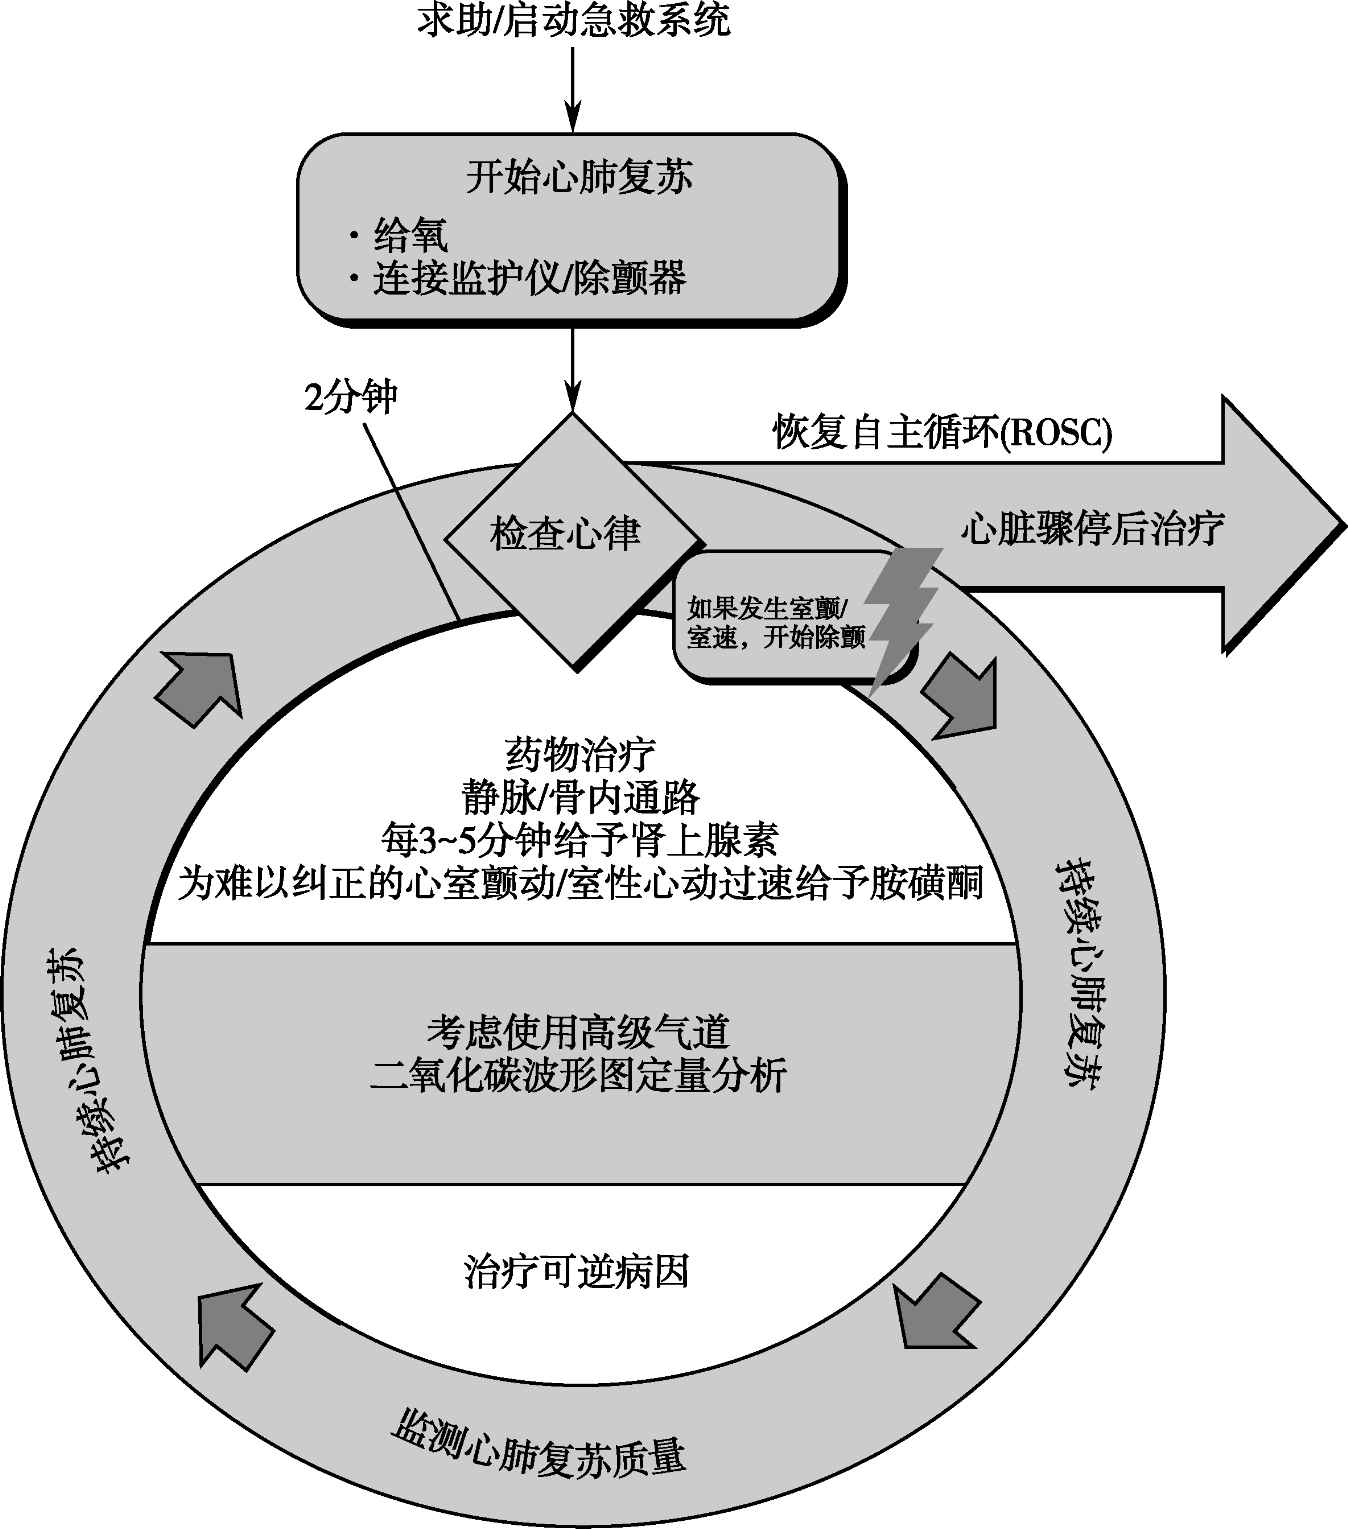
\includegraphics[width=3.9375in,height=4.46875in]{./images/Image00402.jpg}
 \captionsetup{justification=centering}
 \caption{环形成人高级生命支持流程}
 \label{fig101-1}
  \end{figure} 

3.进一步强调了生理参数监测以优化心肺复苏质量并检测是否恢复自主循环。如按压频率及幅度、胸廓回弹恢复、按压中断持续时间、通气频率及幅度,均可作为适时监测和优化CPR质量的指标。

4.不再建议在治疗无脉性心电活动(PEA)/心搏停止时常规性地使用阿托品。

5.建议输注增强节律药物,作为有症状的不稳定型心动过缓进行起搏的替代方法之一。

6.建议使用腺苷,因为它不但安全,而且在未分化的、规则的、单型性、宽QRS波群心动过速的早期处理中,对于治疗和诊断都有帮助。必须注意,腺苷不得用于非规则宽QRS波群心动过速,因为它会导致心律变成室颤。

7.恢复自主循环后,在重症监护病房应继续进行系统的心脏骤停后治疗,同时由专家对患者进行多学科治疗并对其神经系统和生理状态进行评估。这通常包括使用低温治疗。

8.在恢复自主循环后根据氧合血红蛋白饱和度逐渐降低吸氧浓度
,恢复循环后,监测动脉氧合血红蛋白饱和度。如果有适当的装置,应该逐步调整给氧以保证氧合血红蛋白饱和度≥94\%。假设有适当的装置,在恢复自主循环后,应该将吸氧浓度(FIO\textsubscript{2}
)调整到需要的最低浓度,以实现动脉氧合血红蛋白饱和度≥94\%,目的是避免组织内氧过多并确保输送足够的氧。由于氧合血红蛋白饱和度为100\%可能对应肺泡-动脉氧分压差(PaO\textsubscript{2}
)为大约80~500mmHg之间的任意值,所以饱和度为100\%时通常可以取消给予FIO\textsubscript{2}
,前提是饱和度可以保持为≥94\%。

ACLS流程所含的推荐标准如下:①心肺复苏质量:胸外按压,用力(≥5cm),快速(≥100次/分),按压后胸廓回弹恢复;尽可能减少按压中断;避免过度通气;每隔2分钟按压者交换一次;未建立人工气道,采用30∶2按压/通气比率;采用二氧化碳波形图定量分析,如PETCO\textsubscript{2}
< 10mmHg,应提高心肺复苏质量;有创动脉压力,如舒张压<
20mmHg,应提高心肺复苏质量。②ROSC:脉搏和血压;PETCO\textsubscript{2}
迅速持续增高(通常≥40mmHg);有创动脉波监测动脉压变化。③电击能量:双相波,制造商建议值(120~200J),如该值不详,可选最大值;第2次和后续能量相似,也可考虑提高能量;单相波,360J。④药物治疗:静脉/骨髓腔内注射肾上腺素,剂量每3~5分钟1mg;静脉/骨髓腔内注射血管加压素,剂量40U可替代首剂量或第二剂肾上腺素;静脉/骨髓腔内注射胺碘酮,首剂300mg,第二剂150mg。⑤人工气道:喉咽气道或气管插管;呼气末二氧化碳波形图确认和监测气管插管位置;8~10次/分人工呼吸,伴持续心脏按压。⑥可治病因:低血容量、缺氧、酸中毒、低钾/高钾血症、低温、张力性气胸、心脏压塞、中毒、肺栓塞、急性冠脉综合征等。

\subsubsection{2000年以来CPR-ECC指南的更新总汇}

自2000年以第一部国际CPR-ECC指南面貌发布后,科学循证证据的评价使指南成为临床推荐方案的重点;随着科学证据的不断充实,指南内容的不断更新也成为相关学科领域的关注点。2005年CPR-ECC指南对重要技术指标做了重大更改,2010年指南也就相关内容作了更新。为便于比较10年间(2000~2010)指南基本内容的变化,归纳其变化见表\ref{tab101-1}。

\begin{longtable}{c}
 \caption{2000~2010年CPR-ECC指南内容变化比较表}
 \label{tab101-1}
 \endfirsthead
 \caption[]{2000~2010年CPR-ECC指南内容变化比较表}
 \endhead
 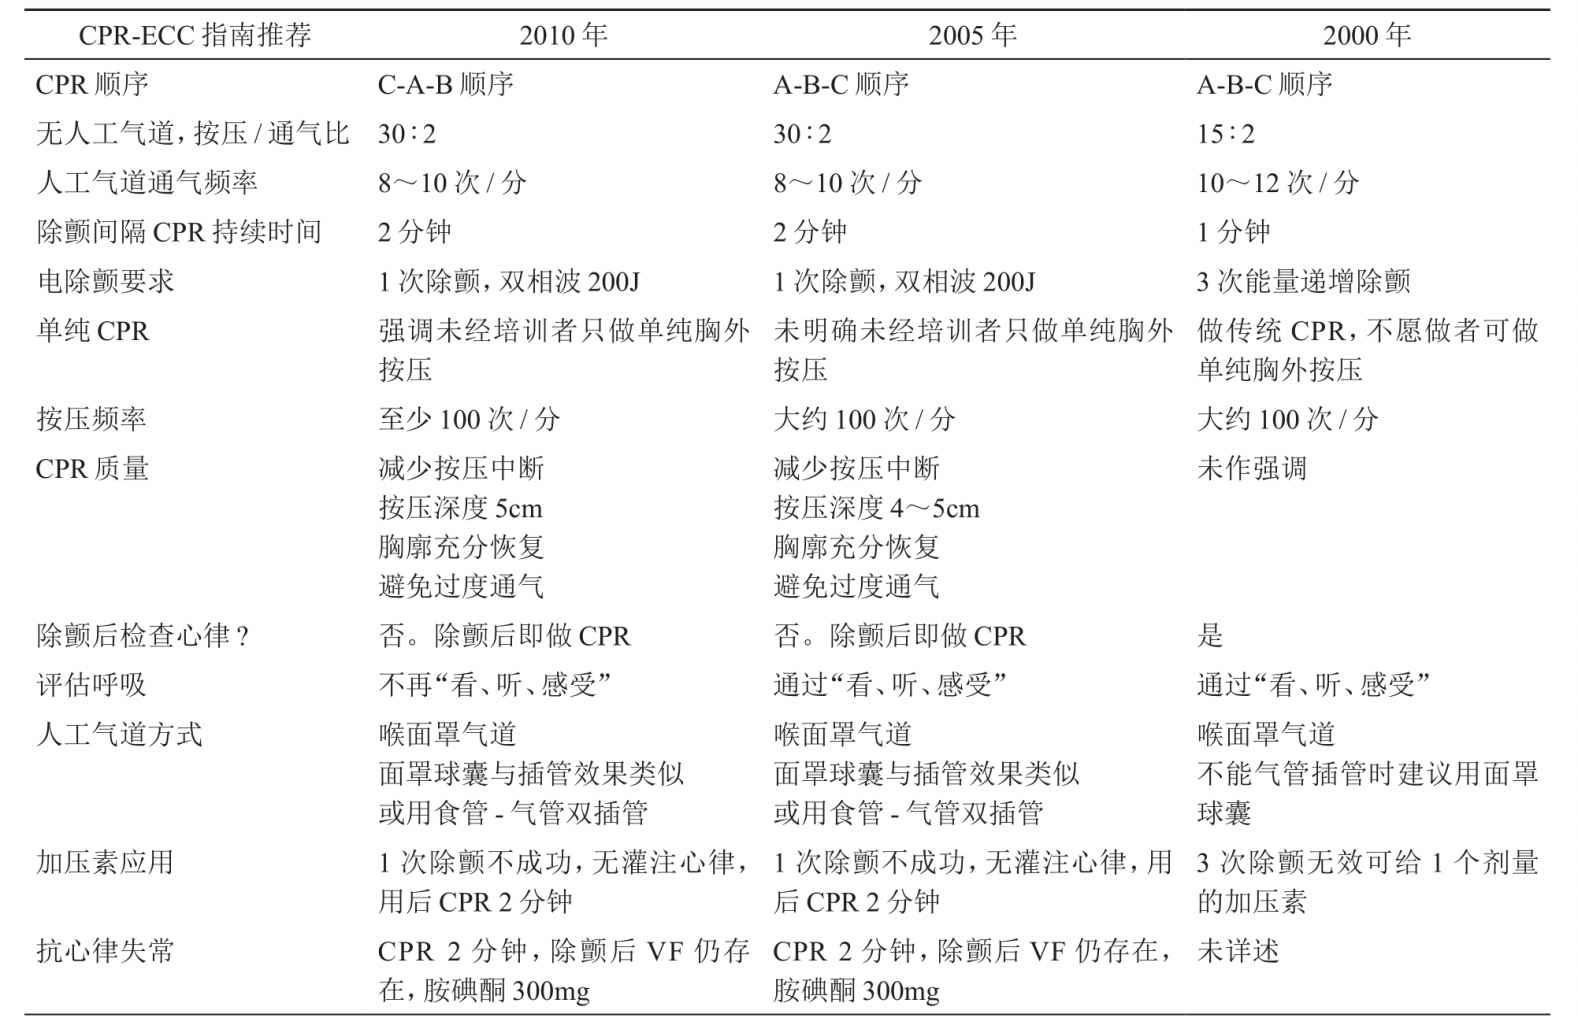
\includegraphics[width=\textwidth,height=\textheight,keepaspectratio]{./images/Image00403.jpg}\\
 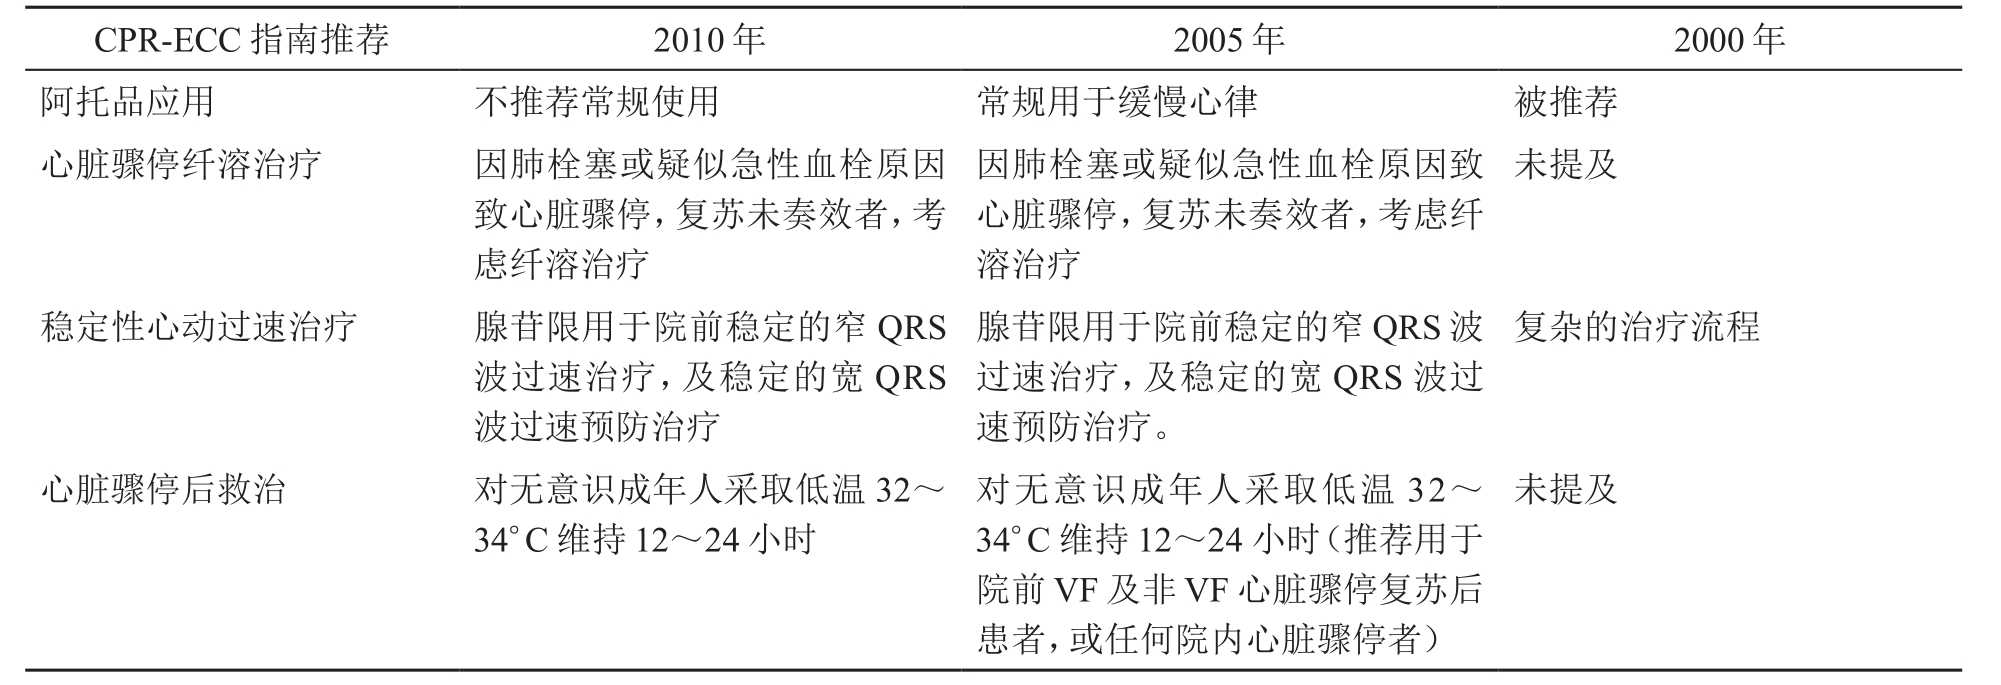
\includegraphics[width=\textwidth,height=\textheight,keepaspectratio]{./images/Image00404.jpg}
 \end{longtable}

\protect\hypertarget{text00283.html}{}{}

\section{基本生命支持}

基本生命支持(basic life
support,BLS)是维持人生命指征的最基本方法和手段,包括对心脏骤停、心脏病发作、卒中和气道异物梗阻的识别,迅速采用胸外心脏按压维持血液循环,人工呼吸给氧和电除颤纠正心律失常。

\subsubsection{BLS与急救医疗服务体系}

人们已经意识到要提高心肺复苏患者的生存率,需要通过院前急救医疗服务系统(EMSS)来实现。这个急救系统是由许多个急救机构和环节结合组成的急救链。其中任何一个环节被打断,都会使救治的最终目标无法实现。它主要由两部分组成------院前急救和院内急救系统。院前急救系统包括:预防急症,识别猝死,实施复苏,将患者转移至急诊科或相应医疗机构。

1992年心肺复苏指南提出“生存链”的基本概念。具体描述了早期识别求救、早期心肺复苏、早期电除颤以及早期高级生命支持。生存链包含的重要原则:①如果生存链中的任何一个环节的薄弱,都将会使生存率降低。②其中“早期识别求救”这一环节最为重要。如果无人发现、识别病情并立即开始求救或抢救的话,患者就不可能获救;早期心肺复苏的有效性决定了是否能成功的关键;早期快速除颤是针对室颤或无脉室速最有效的治疗手段。③整个心脏救治系统的有效性和可靠性不仅通过评价某一环节来确定,而要对整个救治系统进行评价。出院存活率是对心脏急症患者治疗有效性进行评价的标准。2010年指南继续强调,有效BLS是ACLS成功的基础,即开始尽可能少中断的高质量CPR,数分钟内对室颤/无脉VT的电除颤。提出新“生存链”的第五个环节即心脏骤停后救治,强调多学科综合优化救治的重要性。从心脏骤停识别开始,经ROSC后救治,直至存活出院。

新生存链------五个环节:

\paragraph{第一环节}

早期识别、求救。

早期发现心脏性猝死的征兆,如胸痛、气短等,要宣传让患者在发病前向急救医疗服务系统求救是这一环节的关键。一旦发生心脏骤停时,必须快速采取行动:①及时发现患者心脏停搏,如出现“无反应、无呼吸,以及无循环指征”,并快速求救EMS系统;②快速呼叫急救医疗小组(通过电话);③急救调度员应意识到患者出现心脏停搏的可能性;④快速向EMS出诊小组发出指示,并指导他们快速找到患者所在地点;⑤EMS出诊小组快速到达指定地点;⑥EMS出诊小组带着必需的急救设备到达患者身旁,确认心脏停搏。

EMS出诊系统通常由经过BLS和高级生命支持(ACLS)两种培训的急救人员组成。通常第一级人员(包括急救医疗人员和救火队员)先达现场,第一级人员应经过早期除颤培训,这将有利于为二级人员提供更快速、有效的高级心血管生命支持。

\paragraph{第二环节}

早期心肺复苏。

如果现场人员发现患者心脏骤停后应立即开始心肺复苏,这是最简易、最有效的方法。如能在急救人员到达前,现场目击者就已进行心肺复苏,生存率会成倍增加。现场人员对婴儿和儿童的心肺复苏就更有意义。

\paragraph{第三环节}

早期电除颤。

早期除颤在生存链各环节中是最有可能提高生存率的手段。自动体外除颤器(AED)应让尽可能多的人会使用,对提高院前心脏停搏患者的生存机会可能非常关键。AED是容易维修和使用的除颤器,可以自动分析患者的心律,发现需要除颤的心律,自动开始充电,然后通知急救者按下键钮行电除颤。AED可以大大地缩短开始除颤的时间。

\paragraph{第四环节}

早期高级生命支持。

处理心脏停搏中,早期高级生命支持是另外一个关键环节。大多数专家认为,一般由4人组成(2名提供ACLS
和2名提供BLS)的出诊小组可对心脏病患者提供最有效的帮助。

\paragraph{第五环节}

心脏骤停后救治,强调多学科综合优化救治,从心脏骤停识别开始,经ROSC后救治,直至存活出院。

\subsubsection{基本生命支持的程序}

BLS是一系列的操作程序,包括对心跳、呼吸停止的判断,基本循环和呼吸支持等干预的技术。CPR中A、B、C、D,即:A:开放气道;B:人工通气;C:循环支持;D:电除颤。现场急救人员首先要对患者有无反应、有无意识,呼吸和循环体征做出准确判断。只要发现无意识、无呼吸(包括异常呼吸),立即向急救医疗服务系统求救,如果有2名以上急救人员在场,一名应立即实施CPR,另一名则快速求救。心肺复苏的基本程序:识别判断、求救EMSS和心肺复苏(CPR)。

\paragraph{识别判断}

BLS的“识别判断”阶段极其关键,经过准确地识别有无意识、反应,无呼吸即实施CPR(复苏体位、按C-A-B顺序)。正确判断了患者心跳、呼吸停止需要急救人员有迅捷的反应能力,无论是判断过程,还是相继采取的急救措施,时间要求非常短暂、迅速,不超过10秒钟。只要发病地点不存在危险并适合,应就地抢救。急救人员在患者身旁快速判断有无损伤和反应。可轻拍或摇动患者(图\ref{fig101-2}),并大声呼叫:“您怎么了”。如果患者有头颈部创伤或怀疑有颈部损伤,要注意会造成脊髓损伤,对患者不适当地搬动可能造成截瘫。

\begin{figure}[!htbp]
 \centering
 
\includegraphics[width=3.13542in,height=1.54167in]{./images/Image00405.jpg}
 \captionsetup{justification=centering}
 \caption{识别判断患者有无损伤和反应示意图}
 \label{fig101-2}
  \end{figure} 

\paragraph{启动 EMS系统}

如发现患者无反应、无意识及无呼吸,只有一人在现场,对成人要先拨打急救电话,启动EMS系统,目的是求救于专业急救人员,并快速携带除颤器到现场。如果是淹溺或其他因窒息原因所致,应立即进行五组CPR(约2分钟),再去打电话。2人以上时,一人打电话,另一人马上实施CPR。打电话的人要保持平静,不要慌张,准备回答下列问题:①需急救的患者所处位置(街道或路名、办公室名称、房室号);②急救患者所在地电话号码;③发生什么事件,心脏病发作或交通事故等;④所需急救的人数;⑤患者的一般情况;⑥已经给予患者何种急救措施(“正在行CPR”,“正使用AED”);⑦其他任何被询问的信息,确保EMS急救人员无任何疑问。最好在急诊医生对现场救治提出指导后,拨打电话者再挂断电话。

\paragraph{心肺复苏准备}

如果患者无反应,急救人员应判断患者有无呼吸或是否异常呼吸,先使患者取复苏体位(仰卧位),即先行30次心脏按压,再开放气道。患者无反应时,因肌张力下降,舌体和会厌可能把咽喉部阻塞(舌是造成呼吸道阻塞最常见的原因)。有自主呼吸时,吸气过程气道内呈负压,也可将舌或会厌(或两者同时)吸附到咽后壁,造成气道阻塞。如无颈部创伤,可以采用仰头抬颏或托颌法,开放气道,对非专业人员因托颌法难于学习,故不推荐采用,专业急救人员对怀疑有颈椎脊髓损伤的患者,应避免头颈部的延伸,可使用托颌法。

开放气道方法:

\hypertarget{text00283.htmlux5cux23CHP10-1-4-2-3-1}{}
(1) 仰头抬颏法:

完成仰头动作应把一只手放在患者前额,用手掌把额头用力向后推,使头部向后仰,另一只手的手指放在下颏骨处,向上抬颏,使牙关紧闭,下颏向上抬动(图\ref{fig101-3}),匆用力压迫下颌部软组织,以免可能造成气道梗阻。也不要用拇指抬下颏。气道开放后有利于患者自主呼吸,也便于CPR时做口对口人工呼吸。如果患者义齿松动,应取下,以防其脱落阻塞气道。

\begin{figure}[!htbp]
 \centering
 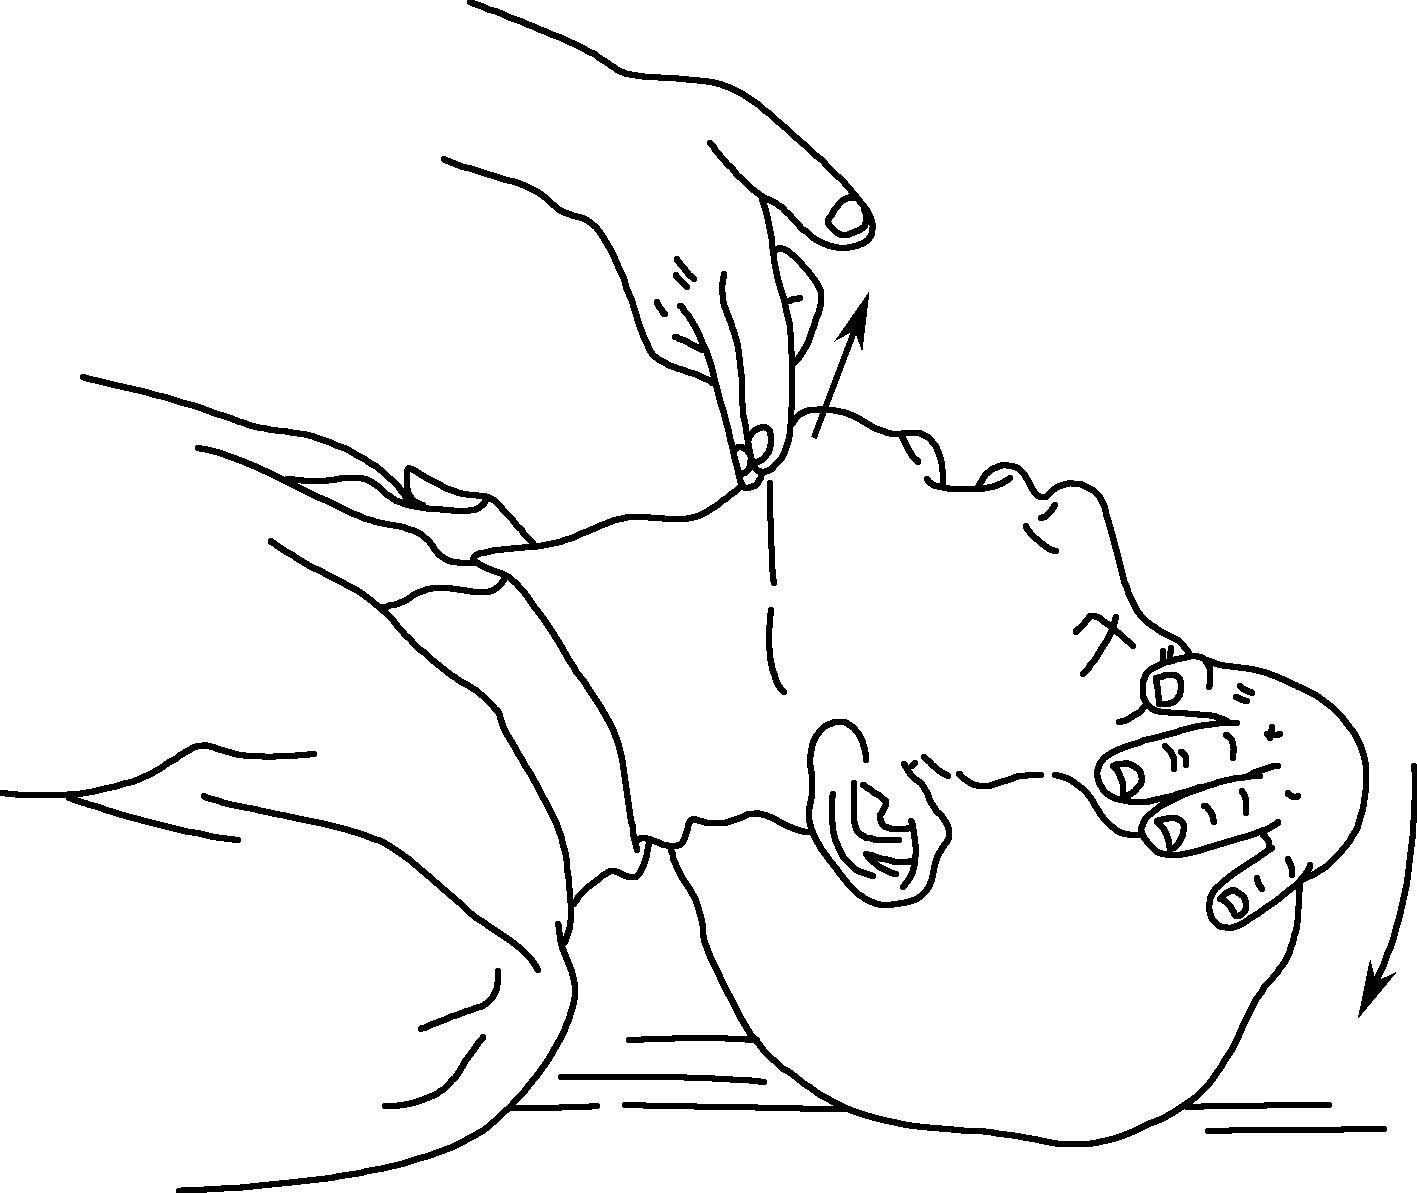
\includegraphics[width=2.35417in,height=1.97917in]{./images/Image00406.jpg}
 \captionsetup{justification=centering}
 \caption{仰头抬颏法示意图}
 \label{fig101-3}
  \end{figure} 

\hypertarget{text00283.htmlux5cux23CHP10-1-4-2-3-2}{}
(2) 托颌法:

把手放置患者头部两侧,肘部支撑在患者躺的平面上,托紧下颌角,用力向上托下颌,如患者紧闭双唇,可用拇指把口唇分开。如果需要行口对口人工呼吸,则将下颌持续上托,用面颊贴紧患者的鼻孔。此法效果肯定,但费力,有一定技术难度。对于怀疑有头、颈部创伤患者,此法更安全,不会因颈部活动而加重损伤。

\subsubsection{人工呼吸}

\paragraph{检查呼吸}

开放气道后,不再推荐采用感觉有无气息(流),观察胸部有无起伏动作,听有无气流呼出的声音的方法。一经观察确定无意识,及无呼吸或出现异常呼吸,即判断为心脏骤停。

绝大多数呼吸或心搏骤停患者均无呼吸,偶有患者出现异常或不规则呼吸,或有明显气道梗阻征的呼吸困难,这类患者开放气道后即可恢复有效呼吸。开放气道后发现仍无呼吸或呼吸异常时,应立即行人工通气,如果不能确定通气是否异常,也应立即进行人工通气。

如果在复苏中或之后患者恢复呼吸和循环体征(有脉搏、正常呼吸、咳嗽或活动),应继续维持呼吸道通畅,此时,患者应处于恢复体位。

\paragraph{人工呼吸}

采用人工呼吸时,每次通气必须使患者的肺脏膨胀充分,可见胸廓上抬。

\hypertarget{text00283.htmlux5cux23CHP10-1-4-3-2-1}{}
(1) 口对口呼吸:

口对口呼吸是一种快捷有效的通气方法,呼出气体中的氧气足以满足患者需求。人工呼吸时,要确保气道通畅,捏住患者的鼻孔,防止漏气,急救者用口把患者的口完全罩住,呈密封状,缓慢吹气,每次吹气应持续1秒以上,确保通气时可见胸廓起伏(图\ref{fig101-4})。

口对口呼吸常会导致患者胃胀气,并可能出现严重并发症,如胃内容物反流,导致误吸或吸入性肺炎,胃内压升高后,膈肌上抬,限制肺的运动。所以应缓慢吹气,不可过快或过用力,减少吹气量及气道压峰值水平,有助于减低食管内压,减少胃胀气的发生。对大多数未建立人工气道的成人,推荐约500~600ml潮气量,既可降低胃胀气危险,又可提供足够的氧合。建立人工气道者400ml潮气量可满足要求。

\begin{figure}[!htbp]
 \centering
 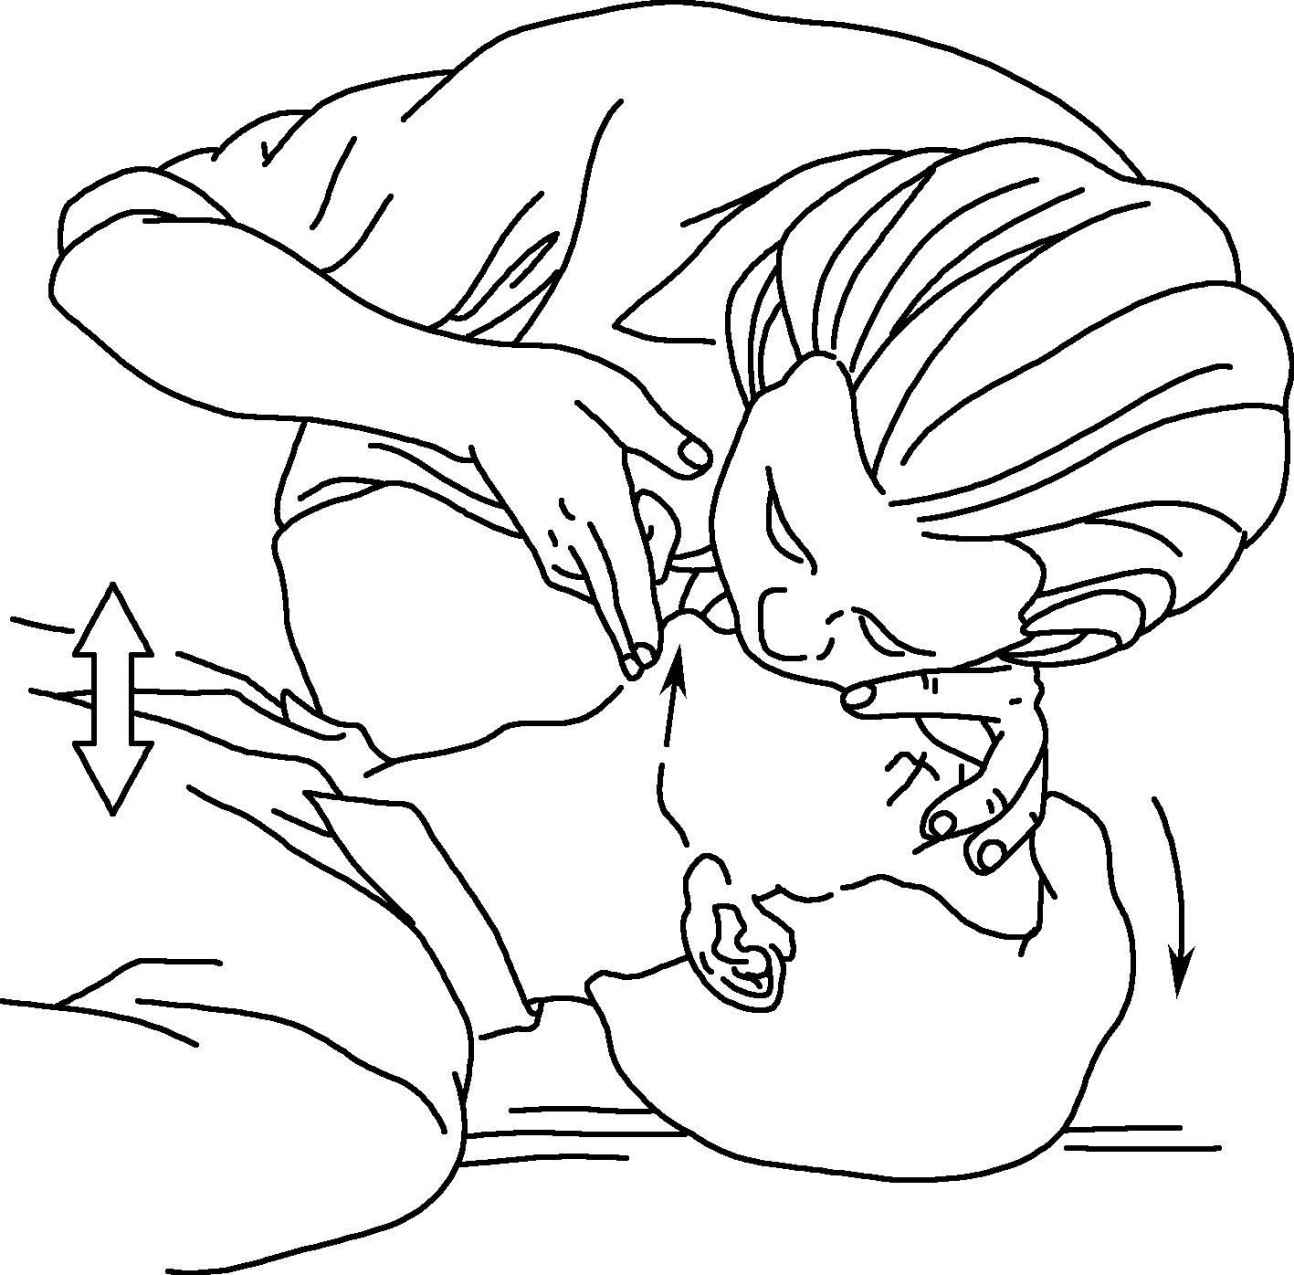
\includegraphics[width=2.35417in,height=2.32292in]{./images/Image00407.jpg}
 \captionsetup{justification=centering}
 \caption{口对口呼吸图示}
 \label{fig101-4}
  \end{figure} 

\hypertarget{text00283.htmlux5cux23CHP10-1-4-3-2-2}{}
(2) 口对鼻呼吸:

口对鼻呼吸适于那些不能进行口对口呼吸的患者,如牙关紧闭不能开口、口唇创伤、口对口呼吸难以实施等。救治溺水者尤其适用口对鼻呼吸方法,只要患者头一露出水面即可行口对鼻呼吸。口对鼻呼吸时,将一只手置于患者前额后推,另一只手抬下颏,使口唇紧闭。用嘴封罩住患者鼻子,吹气后口离开鼻子,让呼气自动排出。必要时,间断使患者口开放,或用拇指分开口唇,这对有部分鼻腔阻塞的患者呼气非常重要。

\hypertarget{text00283.htmlux5cux23CHP10-1-4-3-2-3}{}
(3) 口对气管套管呼吸:

气管切开的患者需人工通气时可采用口对套管呼吸,对套管主动吹气,被动呼气,易于操作。如果气管套管梗阻,且解除梗阻有困难时,要更换新套管;如放置套管出现困难,应立即从皮肤孔道处人工通气。气管套管的套囊可防止通气时漏气,如果发生漏气,用手或面罩把口鼻紧紧封严即可。

\hypertarget{text00283.htmlux5cux23CHP10-1-4-3-2-4}{}
(4) 口对通气防护装置呼吸:

在工作场所,推荐使用有防护装置的通气,以防疾病相互传播。目前有两类装置,口对面罩和面部防护板,口对面罩是单向阀门,因此,患者呼出气进不到急救者的口中;面部防护板没有呼吸阀门,患者呼出气位于患者面部的防护板之间,通气装置气流阻力要低,以免影响患者呼气。

\hypertarget{text00283.htmlux5cux23CHP10-1-4-3-2-5}{}
(5) 口对面罩呼吸:

用透明有单向阀门的面罩,可将急救者呼气吹入患者肺内,有的面罩有氧气接口,以便口对面罩呼吸时同时供给氧气。用面罩通气时双手把面罩贴紧患者面部,这样闭合性好,通气效果非常好。口对面罩通气时有两种疗法,一种是头部法,急救人员位于患者头顶部,此法可用于呼吸骤停而非心跳骤停患者,可以看到胸廓起伏,或两名急救人员在行CPR时的通气位置,托下颌时多用此法。另一方法是急救人员位于患者头侧,仰头抬颏法时多用此法,在一人CPR时比较理想,既可通气,又可行胸外按压。

\hypertarget{text00283.htmlux5cux23CHP10-1-4-3-2-6}{}
(6) 球囊-面罩通气:

使用球囊面罩可提供正压通气,但未建立人工气道容易导致胃膨胀,需要送气时间长,潮气量控制在可见胸廓起伏。但急救中挤压气囊难保不漏气,因此,单人复苏时易出现通气不足,双人复苏时效果较好。双人操作时,一人压紧面罩,一人挤压皮囊通气。如果气道开放不漏气,挤压1L成人球囊1/2~2/3量或2L成人球囊1/3量可获得满意的潮气量。

如果仅单人提供呼吸支持,急救者位于患者头顶。如果没有颈部损伤,可使患者头后仰或枕部填毛巾或枕头,使之处于嗅闻位,便于打开气道,一手压住面罩,一手挤压球囊,并观察通气是否充分,双人球囊面罩通气效果更好。

\subsubsection{循环支持}

\hypertarget{text00283.htmlux5cux23CHP10-1-4-4-1}{}
(一) 检查脉搏

自 1992年以后
,有些研究结果对检查脉搏提出质疑,特别是对非专业人员使用这一方法问题反映更多,因为检查脉搏所需时间较长,而且检查本身的敏感性与特异性均较差。

1.急救者需要花相当长时间检查脉搏,通常绝大多数人,包括非专业人员、医学生、医护辅助人员、医生检查颈动脉所需时间都比标准规定的5~10秒更长。最长达24秒,对VF患者每延迟电除颤1分钟,死亡率可增加7\%~10\%,按以往标准,只有15\%的人能在规定时间内完成脉搏检查。

2.如果把检查颈动脉搏动作为一种诊断手段,①特异性只有90\%,即当患者无脉搏时,仍有10\%的机会被检查者认为有脉搏,这样,在100例患者中,有10例被误认为有脉而失去胸外按压或电除颤的机会,患者最终会因错失复苏的最佳机会而死亡。②敏感性只有55\%,即当患者有脉搏时,有45\%的患者被急救人员认为无脉搏,此时,就有可能错误地进行胸外按压和除颤。③总的准确率只有65\%,错误率35\%。

基于以上结果,2000指南规定对非专业急救人员,在行CPR前不再要求将检查颈动脉搏动作为一个必须的诊断步骤。因此,非专业急救人员无需根据脉搏检查结果来确定是否需要胸外按压或电除颤,如果发现无反应、无自主呼吸即按心脏骤停处理;对于专业急救人员如检查脉搏,但不能超过10秒,如不能确定有无脉搏,应立即进行CPR。

\hypertarget{text00283.htmlux5cux23CHP10-1-4-4-2}{}
(二) 检查循环体征

评价循环体征
,对非专业人员来说是指以下内容:给予人工呼吸并评价患者的正常呼吸、咳嗽情况,以及对急救通气后的运动反应。对专业急救人员,检查循环体征时,要一方面检查颈动脉搏动,一方面观察呼吸、咳嗽和运动情况,专业人员能鉴别正常呼吸、濒死呼吸,以及心脏骤停时其他通气形式。

评价时间不要超过10秒,如果不能肯定是否有循环,则应立即开始胸外按压。1岁以上的患者,颈动脉比股动脉更易触及,方法是患者仰头后,急救人员一手按住前额,用另一手的示、中手指找到气管,两指下滑到气管与颈侧肌肉之间的沟内即可触及颈动脉(图\ref{fig101-5})。

\hypertarget{text00283.htmlux5cux23CHP10-1-4-4-3}{}
(三) 胸外按压

CPR时胸外按压部位在胸骨1/2处进行按压,要求按压可产生60~80mmHg收缩期峰压,通过增加胸内压或直接挤压心脏产生血液流动,通过胸外按压使血液流向肺脏,并辅以适当的呼吸,就可为脑和其他重要器官提供充足的氧气,以便行电除颤。

\begin{figure}[!htbp]
 \centering
 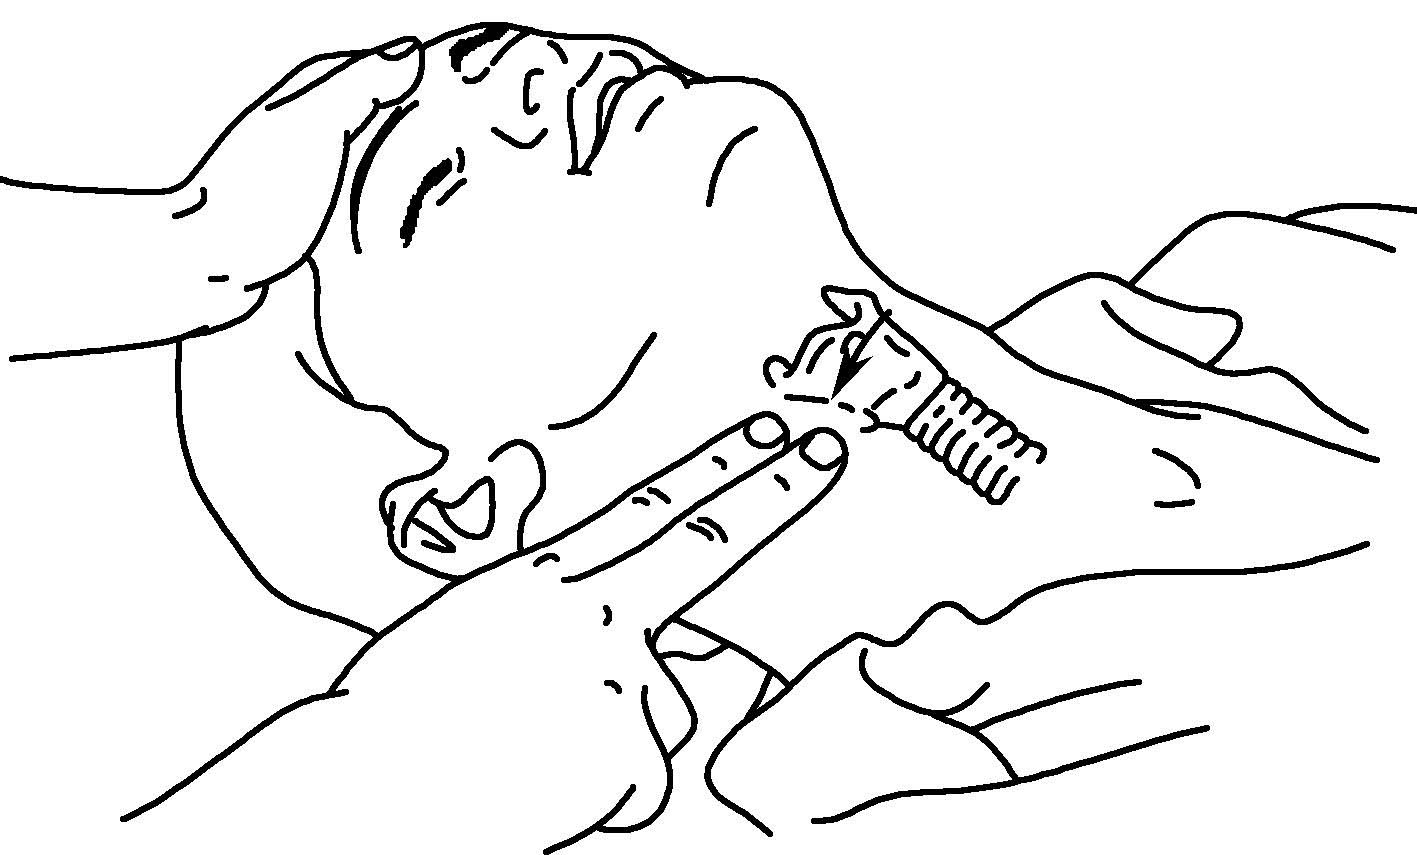
\includegraphics[width=2.35417in,height=1.41667in]{./images/Image00408.jpg}
 \captionsetup{justification=centering}
 \caption{评价循环体征}
 \label{fig101-5}
  \end{figure} 

2010年专家达成共识:①CPR时为保证组织器官的血流灌注,必须实施有效的胸外按压。②有效的胸外按压必须快速、有力。成人按压频率至少100次/分,按压深度不少于5cm,每次按压后胸廓完全回复,按压与放松比大致相等。③尽量避免胸外按压的中断。④在建立人工气道前,成人单人CPR或双人CPR,按压/通气比率都为30∶2,气管插管以后,按压与通气可能不同步,通气8~10次/分,按压频率大于100次/分,这要求平时采取措施加强训练。

\paragraph{胸外按压技术}

患者应仰卧平躺于硬质平面,术者跪在其旁。若胸外按压在床上进行,应在患者背部垫以硬板。按压部位在胸骨下半部,即双乳头连线与胸骨交界处。用一只手掌根部置于按压部位,另一手掌根部叠放其上,双手指紧扣进行按压。使身体稍前倾,使肩、肘、腕位于同一轴线上,与患者身体平面垂直。用上身重力按压,按压与放松时间相同。每次按压后胸廓完全回复,但放松时手掌不离开胸壁。

\paragraph{有效按压的标准}

①肘关节伸直,上肢呈一直线,双肩正对双手,以保证每次按压的方向与胸骨垂直。如果按压时用力方向不垂直,有可能造成身体滚动,影响按压效果。②对正常形体的患者,按压胸壁的下陷幅度为5cm以上,为达到有效的按压,可根据体形大小增加或减少按压幅度,最理想的按压效果是可触及颈或股动脉搏动。但按压力量以按压幅度为准,而不仅仅依靠触及到脉搏。③每次按压后,放松使胸骨恢复到按压前的位置,血液在此期间可回流到胸腔,放松时双手不要离开胸壁,一方面使双手位置保持固定,另一方面,减少直接对胸骨本身的冲击力,以免发生骨折。按压频率至少100次/分。④按压与放松间隔比为50\%时,可产生有效的脑和冠状动脉灌注压。⑤在连续30次按压周期内,保持双手位置固定,不要改变手的位置,也不要将手从胸壁上移开,每次按压后,使胸廓重新恢复到原来的位置。

研究表明,胸外按压时,血流产生的机制包括胸泵机制和心泵机制(直接对心脏的按压)。在CPR期间,CPR的时间长短可影响血流产生的机制,短时间的CPR,血流更多地是由直接按压心脏产生。心脏停跳时间较长或胸外按压时间较长时,心脏顺应性减低,胸泵机制则占优势。此时,胸外按压产生的心排出量明显减低。

心脏骤停期间,标准而有效的胸外按压可产生峰值达60~80mmHg的动脉压力,但舒张压力较低,颈动脉平均压可超过40mmHg,胸外按压时的心排出量仅为正常心排出量的1/3或1/4,而且,随着CPR时间延长进一步减低,只有按照标准进行按压,才能达到最理想的按压效果。

\paragraph{仅胸外按压的 CPR}

如果旁观者未经过心肺复苏培训,则应进行单纯胸外按压的心肺复苏,即仅为突然倒下的成人患者进行胸外按压并强调在胸部中央用力快速按压,或者按照急救调度的指示操作。施救者应继续实施单纯胸外按压心肺复苏,直至AED到达且可供使用,或者急救人员或其他相关施救者已接管患者。所有经过培训的非专业施救者应至少为心脏骤停患者进行胸外按压。另外,如果经过培训的非专业施救者有能力进行人工呼吸,应按照30次按压对应2次呼吸的比率进行按压和人工呼吸。

单纯胸外按压(仅按压)心肺复苏对于未经培训的施救者更容易实施,而且更便于调度员通过电话进行指导。另外,对于心脏病因导致的心脏骤停,单纯胸外按压心肺复苏或同时进行按压和人工呼吸的心肺复苏的存活率相近。

另有研究表明,成人CPR最初6~12分钟,并非一定需要正压通气。比利时脑复苏研究小组研究表明,CPR期间,接受口对口通气和单行胸外按压的复苏效果无任何区别。还有研究认为,在CPR期间,随胸廓按压起伏时的自动通气,可维持接近正常时分钟通气量、PaCO\textsubscript{2}
和PO\textsubscript{2}
,而无需正压通气,因为胸外按压时的心排出量只有正常的25\%,因而,也减低了维持通气灌流比所需的通气量。

\paragraph{咳嗽 CPR}

这是启动本身自主的CPR,这在理论上是可能的,但在临床应用有一定限制。临床上要求严密监护患者,心脏骤停一定要在目击下发生,在患者意识丧失之前要能用力咳嗽,而且这一情况只有在心脏骤停前的10~15秒可行。咳嗽可使患者胸内压升高,使血流继续流动,以保持清醒的意识。

\paragraph{电击除颤}

大多数成人突发非创伤性心脏骤停的原因是VF,电除颤是救治VF最为有效的方法。早期电除颤也是SCA患者复苏成功的关键。心律分析证实为VF/无脉性VT应立即作1次电除颤,之后做5组CPR,再检查心律,必要时再次除颤。单相波除颤器首次电击能量选择360J,双相波除颤器首次电击能量选择150J或200J。心脏静止与无脉电活动电除颤均无益。

如果任何施救者目睹发生院外心脏骤停且现场有AED,施救者应从胸外按压开始心肺复苏,并尽快使用AED。在医院和其他机构使用现场的AED或除颤器治疗心脏骤停的医务人员应立即进行心肺复苏,并且尽可使用准备好的AED/除颤器。以上建议旨在支持尽早进行心肺复苏和早期除颤,特别是在发生心脏骤停时现场有AED或除颤器的情况下。如果院外心脏骤停的目击者不是急救人员,则急救人员可以开始心肺复苏,同时使用AED或通过心电图检查节律并准备进行除颤。在上述情况下,可以考虑进行1½~3分钟的心肺复苏,然后再尝试除颤。如果有两名或三名施救者在场,应进行心肺复苏,同时拿到除颤器。

对于院内心脏骤停,没有足够的证据支持或反对在除颤之前进行心肺复苏。但对于有心电监护的患者,从心室颤动到给予电击的时间不应超过3分钟,并且应在等待除颤器就绪时进行心肺复苏。

\subsubsection{气道异物梗阻的识别和处理}

气道异物阻塞(foreign body airway
obstruction,FBAO)是一种急症,如不及时治疗,数分钟内就可导致死亡。FBAO造成的心脏骤停并不常见,但有意识障碍或吞咽困难的老年人和儿童发生人数相对较多。FBAO是可以预防和避免发生的。

\paragraph{FBAO的原因及预防}

任何患者突然呼吸骤停都应考虑到FBAO,尤其是年轻患者,呼吸突然停止,出现发绀,无任何原因的意识丧失。成人通常在进食时易发生,肉类食物是造成FBAO最常见的原因。易导致FBAO的诱因有:吞食大块难咽食物,饮酒后,老年人戴义齿或吞咽困难,儿童口含小颗粒状食品或物品。注意下列事项有助于预防FBAO:①将食物切碎,细嚼慢咽,尤其是戴义齿者;②咀嚼和吞咽食物时,避免大笑或交谈;③避免酗酒;④阻止儿童口含食物行走、跑或玩耍;⑤将易误吸入的异物放在婴幼儿拿不到处;⑥不宜给小儿需要仔细咀嚼或质韧而滑的食物(如花生、坚果、玉米花、果冻等)。

\paragraph{FBAO的识别}

异物可造成呼吸道部分或完全阻塞,识别FBAO是抢救成功的关健。部分阻塞时,患者有通气,能用力咳嗽,但在咳嗽停止时,出现喘息声。此时救助者不宜干扰患者自行排除异物的努力,而应鼓励患者继续咳嗽并自主呼吸。但应守护在患者身旁,并监护患者的情况,如不能解除,即求救EMSS。

FBAO患者可能一开始就表现为通气不良;或开始通气好,但逐渐恶化,表现为乏力、无效咳嗽、吸气时高调嗓音、呼吸困难加重、发绀。对待这类患者要同气道完全阻塞一样,须争分夺秒地救治。

气道完全阻塞的患者,不能讲话,不能呼吸或咳嗽,用双手抓住颈部,无法通气。对此征象必须能立即明确识别。救助者应马上询问患者是否被异物噎住,如果患者点头确认,必须立即救治。如不能迅速解除气道阻塞,患者将很快出现意识丧失,甚至死亡。如遇患者意识已丧失,猝然倒地,则应立即CPR。

\paragraph{解除FBAO}

常用方法有:

\hypertarget{text00283.htmlux5cux23CHP10-1-4-5-3-1}{}
(1) 腹部冲击法(Heimlich法):

腹部冲击法可使膈肌抬高,气道压力骤然升高,促使气体从肺内排出,这种压力足以产生人为咳嗽,把异物从气管内冲击出来。适用于有意识的立位或坐位患者。救助者站在患者身后,双臂环抱患者腰部,一手握拳,握拳手的拇指侧紧抵患者腹部,位于剑突下与脐上的腹中线部位,再用另一手抓紧拳头,用力快速向内、向上使拳头冲击腹部,反复冲击直到把异物从气道内排出来。如患者意识丧失,即开始CPR。虽腹部冲击法卓有成效,但也可产生并发症,如腹部或胸腔内脏的破裂或撕裂,1岁以下婴儿,除非必要时,一般不随便采用此法。对已行腹部冲击法治疗的患者应仔细检查有无危及生命的并发症。

\hypertarget{text00283.htmlux5cux23CHP10-1-4-5-3-2}{}
(2) 自行腹部冲击法:

发生FBAO时,患者本人可一手握拳,用拳头拇指侧抵住腹部剑突下与脐上腹中线部位,另一只手抓紧拳头,用力快速向上、向内使拳头冲击腹部。如果不成功,患者应快速将上腹部抵压在一硬质的物体上,如椅背、桌缘、走廊栏杆,然后用力冲击腹部,直到把气道内异物排除。

\hypertarget{text00283.htmlux5cux23CHP10-1-4-5-3-3}{}
(3) 胸部冲击法:

当患者是妊娠终末期或过度肥胖者时,可采用胸部冲击法代替腹部冲击法。其方法是,救助者站在患者身后,把上肢放在患者腋下,将胸部环抱住。一只拳的拇指则放在胸骨中线,应注意避开剑突和肋骨下缘,另一只手抓住拳头,向后冲击,直至把异物排击。

\hypertarget{text00283.htmlux5cux23CHP10-1-4-5-3-4}{}
(4) 对意识丧失者的解除方法:

在解除FBAO期间发生意识丧失,救助者应立即求救EMSS(或让其他人去启动EMSS)并开始CPR。胸部按压有助于无反应患者解除FBAO。对专业急救人员,如怀疑意识丧失是由FBAO引起的,建议采取下列方法:①在CPR过程中,如有第二名急救人员在场,则让其启动EMSS。患者保持平卧。②用舌-上颌上提法开放气道,并试用手指清除口咽部异物。③开放气道,尝试通气,如通气时患者胸部无起伏,重新摆放头部位置,再尝试通气。④如果反复尝试后仍不能进行有效通气,则应考虑FBAO。此时,骑跨在患者膝部,实施腹部冲击法(可连续冲击5次)。⑤在异物清除前,如果通气仍不能使胸廓起伏,应考虑进一步的抢救措施(如Kelly钳,Magilla镊,环甲膜穿刺/切开术),建立通畅的气道。⑥如FBAO已去除,气道开通后患者仍无呼吸,需2次人工通气。再检查循环体征(检查脉搏及自主呼吸、咳嗽和运动),如无脉搏,即开始胸外按压。按压/通气比30∶2。

\subsubsection{与CPR有关的其他问题}

\hypertarget{text00283.htmlux5cux23CHP10-1-4-6-1}{}
(一) CPR中更换场所

如果事发现场不安全,如失火建筑,则应把患者转移到安全区域,然后立即开始CPR。在实施有效的CPR使患者循环重新恢复之前,或其他急救人员到来前,不应图方便而把患者从拥挤或繁忙的区域向别处转移。只要有可能,就别中断CPR。

\paragraph{楼梯}

运输患者有时需上下楼梯,最好在楼梯口进行CPR,预先规定好转运时间,尽可能快地转至下一个地方,之后立即重新开始CPR,CPR中断时间尽可能短,且尽可能避免中断。

\paragraph{担架}

在将患者转至救护车或其他移动性救护设备途中,仍不要中断CPR,如果担架较低,急救人员可跟随在担架旁边,继续实施胸外按压;如果担架或床较高,急救人员应跪在担架或床上,以达到患者胸骨的高度,便于CPR。一般情况下,只有在专业人员气管插管时,或应用AED或手动除颤时,或转运途中出现问题时,才能中断CPR,如果只有一个急救人员,为启动EMS系统,可停一会儿CPR。

\hypertarget{text00283.htmlux5cux23CHP10-1-4-6-2}{}
(二) BLS易发生的问题和并发症

如果CPR措施得当,就可为患者提供生命支持。有时即使正确实施CPR,也可能出现并发症,然而,不能因为害怕出现并发症就不最大限度地进行CPR。

\paragraph{人工呼吸的并发症}

急救人工呼吸时,由于过度通气和通气流量过快,都易发生胃扩张,尤其是儿童更易发生胃扩张,通过维持通畅的气道,限制通气容量,调节通气容量足以使胸廓起伏即可。这样,才能最大限度降低胃扩张发生率。建议缓慢行人工呼吸,在呼气和吸气过程中,要确保气道通畅,也可进一步减轻胃扩张。单人CPR不易做到,而双人CPR可达到以上要求。如有可能,另一人应在急救呼吸时压迫环状韧带,也可以减少胃扩张。明显的胃扩张可引发胃内容物反流,而且,由于胃扩张,膈肌抬高,使肺容量降低。如果急救人工通气期间发生胃膨胀,要重新检查并重新开放气道,并观察在通气时胸廓是否有起伏。避免导致气道压力升高因素(快速呼吸、缩短吸气时间、用力通气),如果发生胃扩张,应继续缓慢通气,别试图排除胃内容物,经验表明,如果想用手按压患者上腹部解除胃扩张,常可导致胃内容物反流。如果出现胃内容物反流,将患者安置侧位,清除口内反流物后,再使患者平卧位,继续CPR。

\paragraph{胸外按压的并发症}

正确的CPR技术可减少并发症,在成人患者,即使胸外按压动作得当,也可造成肋骨骨折,但婴儿和儿童,却很少发生肋骨骨折。胸外按压的其他并发症包括:肋骨骨折、肋骨从胸骨分离、气胸、血胸、肺挫伤、肝脾撕裂伤和脂肪栓子。按压过程中,手的位置要正确,用力要均匀有力,虽然有时可避免一些并发症,但不能完全避免。

\begin{figure}[!htbp]
 \centering
 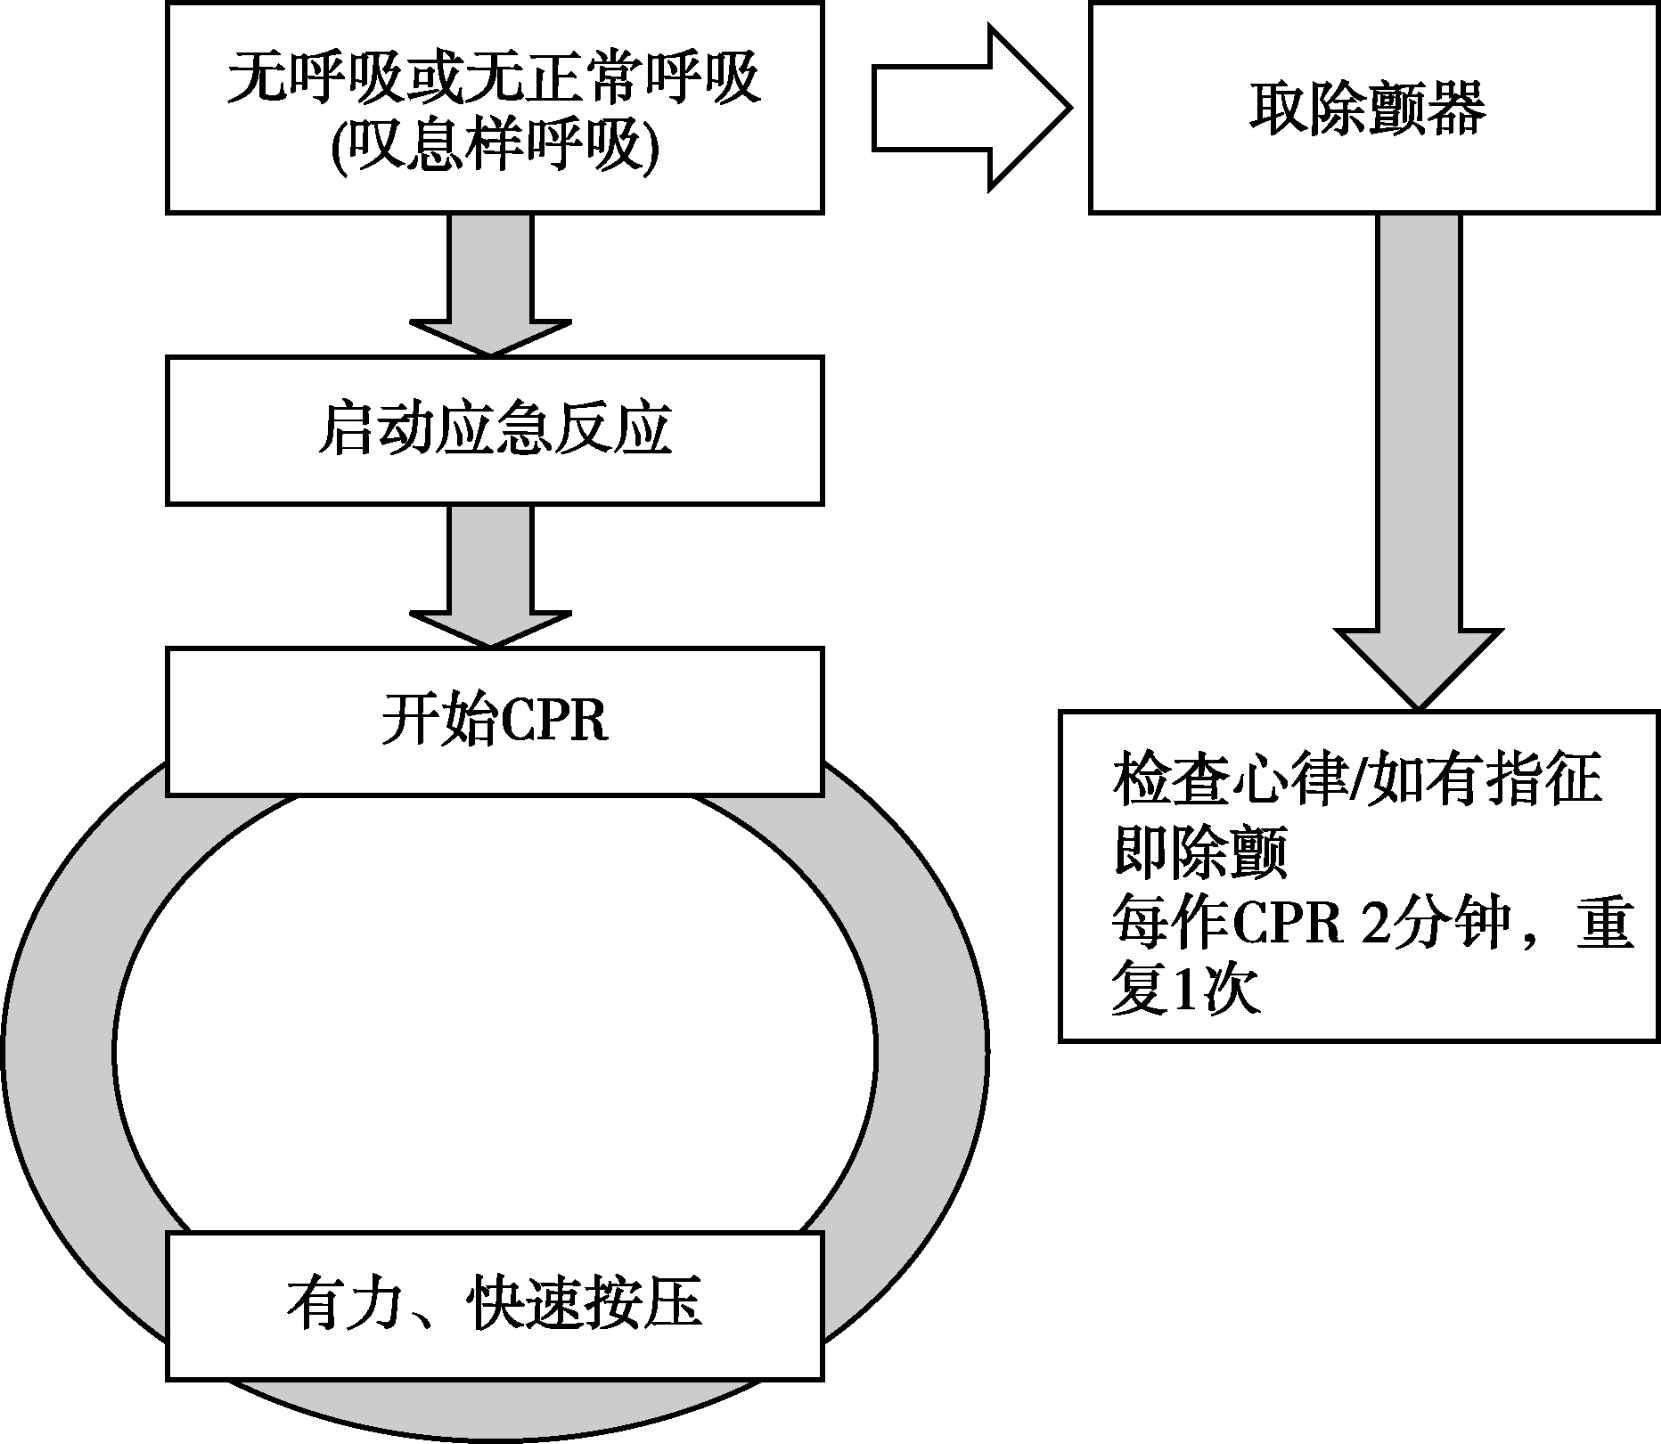
\includegraphics[width=3.10417in,height=2.69792in]{./images/Image00409.jpg}
 \captionsetup{justification=centering}
 \caption{非专业人员成人基础生命支持简化流程}
 \label{fig101-6}
  \end{figure} 

2010
CPR指南制订的非专业人员的成人基础生命支持流程见图\ref{fig101-6};专业医务人员的成人基础生命支持流程见图\ref{fig101-7};成人、儿童和婴儿的关键基础生命支持步骤的总结见表\ref{tab101-2}。

\begin{figure}[!htbp]
 \centering
 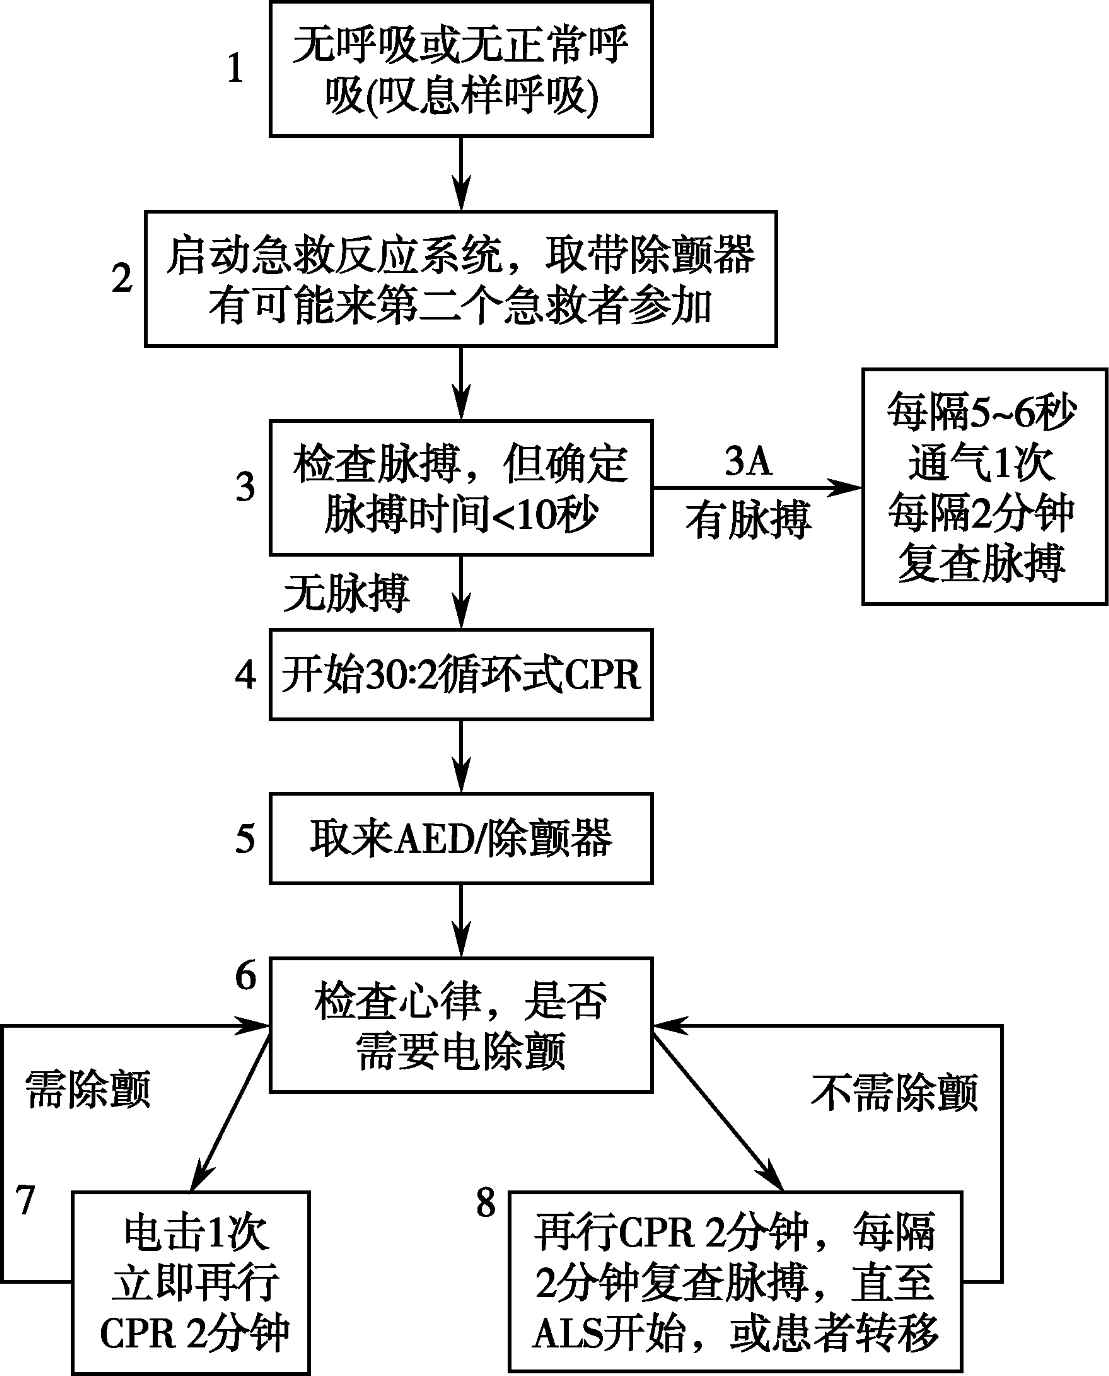
\includegraphics[width=2.92708in,height=3.63542in]{./images/Image00410.jpg}
 \captionsetup{justification=centering}
 \caption{专业医务人员成人基础生命支持简化流程}
 \label{fig101-7}
  \end{figure} 

\begin{table}[htbp]
\centering
\caption{成人、儿童和婴儿的关键基础生命支持步骤的总结}
\label{tab101-2}
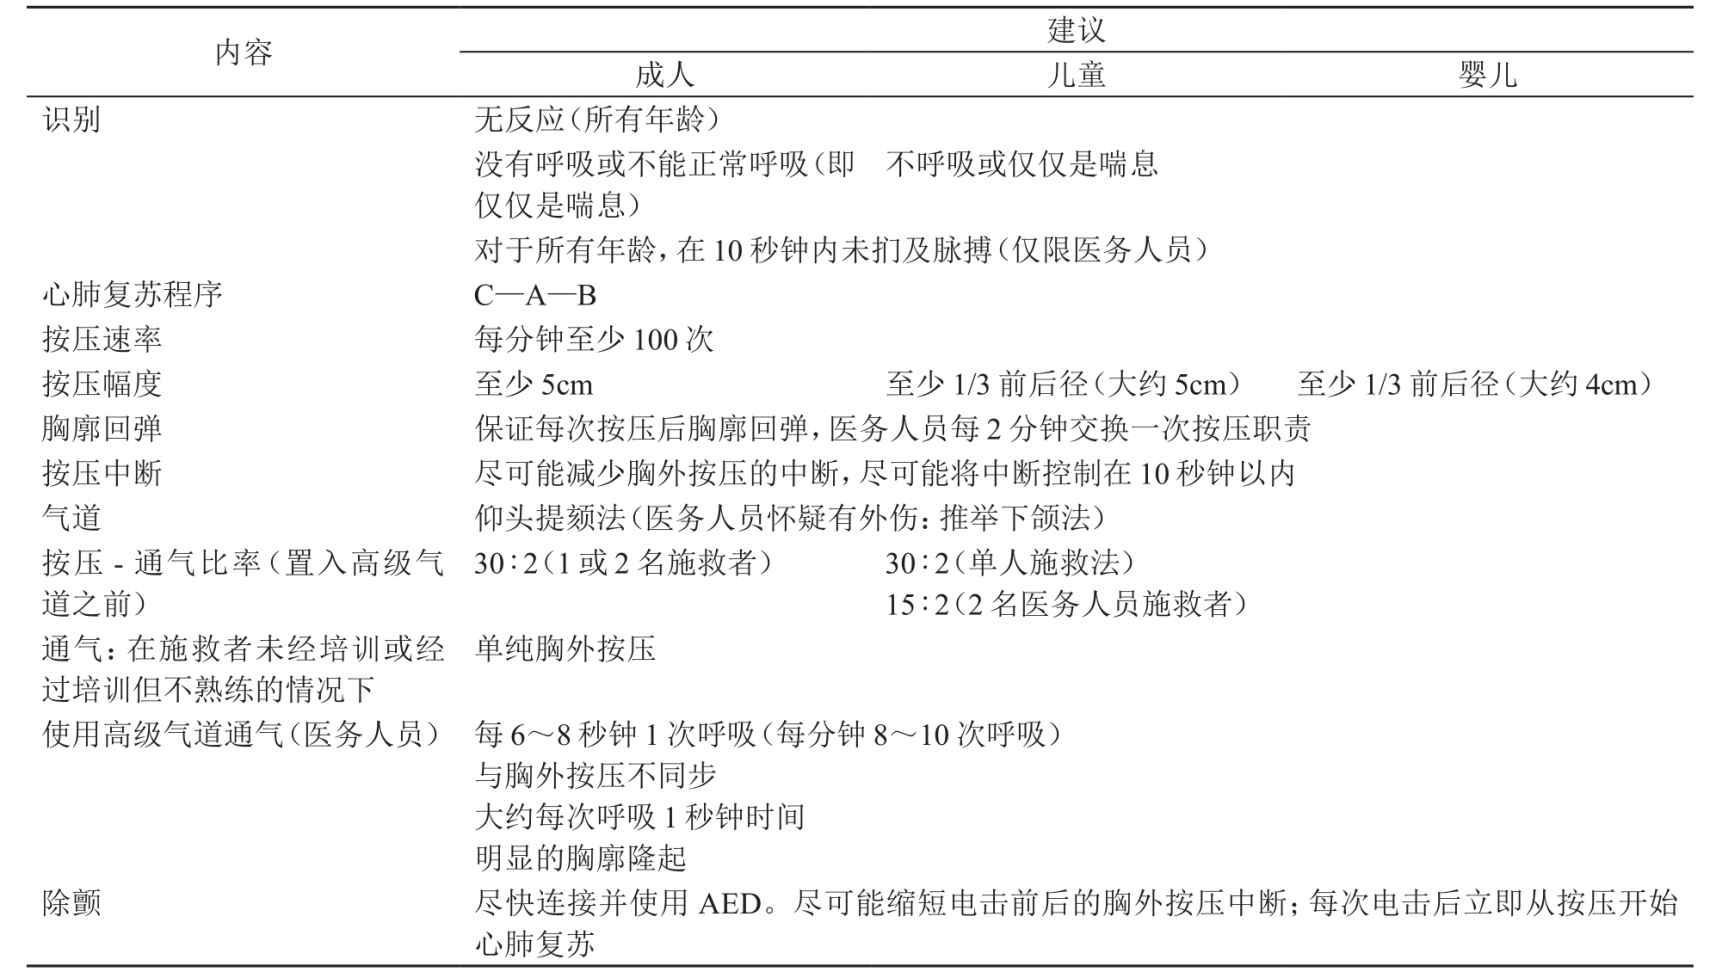
\includegraphics[width=6.66667in,height=3.78125in]{./images/Image00411.jpg}
\end{table}

\protect\hypertarget{text00284.html}{}{}

\section{高级生命支持}

高级生命支持(advanced cardiovascular life
support,ACLS)是在BLS的基础上,为使自主循环恢复和(或)呼吸、循环功能维持或稳定,进一步采取救治措施。

\subsubsection{ACLS主要原则}

\hypertarget{text00284.htmlux5cux23CHP10-1-5-1-1}{}
(一) 时间的重要性

时间决定了心血管急救的各方面,随着心肺功能衰竭状态的持续,生存的可能性明显下降。基本生命支持(BLS)虽能给脑和心脏提供一定的血供,如气管插管、清理阻塞的呼吸道及电除颤等。然而,CPR持续时间越长,对患者则越不利。

\hypertarget{text00284.htmlux5cux23CHP10-1-5-1-2}{}
(二) 心脏停搏前阶段

急症的心血管监护不只局限于心脏停搏的患者,必须对即将发生心脏性猝死和复苏后恢复的患者有足够认识和有效的治疗,如果急救人员在“停搏前阶段”能够及时处理关键病情,则可防止发生心脏停搏。

以下是一个国际ACLS组织基于科学临床指南和某些教学资料制订的心脏停搏前的情况:①急性冠脉综合征;②急性肺水肿、低血压、休克;③有症状的心动过缓;④稳定及不稳定的心动过速;⑤急性缺血性卒中;⑥复苏后再次出现心率、心律、心脏功能的障碍(定义为停搏前状态)。

CPR和ECC指南的其他部分主要强调更特殊原因的心脏停搏,如:电解质异常,药物中毒或过量,以及吞咽毒物所致。

\hypertarget{text00284.htmlux5cux23CHP10-1-5-1-3}{}
(三) 以患者为主

心肺复苏要求急救人员能够快速做出决定
,这一点是很具有挑战性的。急救人员必须在短时间内将注意力集中在复苏过程中的某些特殊方面:如开通静脉通路,进行气管插管,明确心脏节律并及时下达正确医嘱。但急救人员也必须时常注意调整复苏全过程的每个步骤。复苏流程图可使初级急救人员学习掌握复苏步骤中的最主要的内容:如开放气道、辅助通气、CPR、电除颤、药物处理及在特定条件下有利于患者的一切处理。

\subsubsection{初级及高级的ABCD程序}

所有参加心肺复苏的人员,均应以一种简练易记的方式进行训练。“ACLS训练程序”阐明了初步及高级急诊心血管处理的程序,它包括2部分,每部分各有A、B、C、D四个步骤(共八个步骤)。在每个步骤中,救护人员先进行评估,如果评估是适合的,则开始处理。

初级ABCD程序需要双手(且要戴手套)、CPR的隔离设施和一个供除颤使用的AED。其具体步骤如下:

A------气道 用非侵入技术评估和管理气道;

B------呼吸 应用正压通气来评估和管理呼吸;

C------循环 评估和管理循环系统,在AED到达之前持续进行CPR;

D------除颤
评估和管理除颤,判断心脏的节律是否是VF/VT,必要时应给予安全有效的电除颤。

高级复苏的指导程序需要更高级的治疗及侵入性技术,以便进一步评估和处理患者。救护人员希望维持自主呼吸和循环,以便使患者成功获救;继续评估和处理患者,直到专业救护人员赶到。简而言之,高级复苏的指导程序是:复苏-稳定病情-转送到更高水平监护中心。其具体步骤如下:

A------气道评估和处理 高级救护用气管插管建立人工气道;

B------呼吸评估和处理
通过检查插管的位置及工作情况评估呼吸和通气是否充分,纠正发现所有问题,通过用正压通气治疗通气不足来处理呼吸。二氧化碳波形图监测可以评估复苏的效果。

C------循环
通过以下步骤评估和处理循环和用药情况:①开始建立外周静脉通路;②连接ECG导联,以检查ECG是否出现引起心脏骤停的心律失常(VF,无脉VT,无收缩和PEA);③依据心律进行适宜的药物治疗。

D------鉴别诊断
对导致心脏骤停的可能原因做出尽早的分析和判断,以确定其主要原因。

\subsubsection{呼吸支持方法}

\hypertarget{text00284.htmlux5cux23CHP10-1-5-3-1}{}
(一) 供氧

心肺复苏时
,立即行人工呼吸,此时急救者吹入患者肺内是含16\%~17\%氧的空气,理想时肺泡内氧分压可达80mmHg。心脏骤停或心肺复苏时,低心排血量、外周氧释放障碍及大的动静脉血氧差均可导致组织缺氧;其他因素还包括通气异常所致的肺内分流及呼吸系统疾病。组织缺氧导致无氧代谢和代谢性酸中毒,而化学药品及电解质治疗也会对酸碱平衡产生影响。基于上述原因,BLS和ACLS时推荐吸入100\%的纯氧。高氧分压可以增加动脉血中氧的溶解度,进而加大身体氧的输送(=心排血量×血氧浓度);短时内吸入100\%纯氧治疗对人体有益无害,但长时间吸入高浓度氧会产生氧中毒。在急性心肌梗死患者中,氧支持疗法可改善心电图ST段改变的幅度和范围。目前推荐对疑有急性冠状动脉综合征患者,在最初2~3小时内经鼻导管吸氧4L/min;对于持续或反复心肌缺血,或伴充血性心衰、心律失常的复杂心梗,给吸氧3~6小时,直到患者低氧血症纠正,临床上病情稳定。已有研究认为,如果能使氧饱和度保持在94\%以上,尽可能使用较低的给氧浓度,相比较供给100\%氧对神经系统预后更佳。

\hypertarget{text00284.htmlux5cux23CHP10-1-5-3-2}{}
(二) 人工通气

\paragraph{面罩通气}

对训练有素的急救人员来说,应用适合的面罩可以有效而简便地进行人工通气。使用透明面罩可便于观察到胃的反流。面罩需封严面部,同时罩住口、鼻,但有一个提供氧的入口和15~22mm大小的连接头。应备有不同型号的面罩以适合成人及儿童使用。用口-面罩通气时,推荐采用单向阀装置,这样可避免患者呼出气体与急救者口腔接触;与球囊-面罩相比,更易于控制潮气量。为使口-面罩密封效果达到理想,急救人员最好位于患者头端,用嘴密封面罩进气孔对患者吹气,用双手固定面罩,将头部侧倾以保持气道通畅。

\paragraph{球囊 -瓣装置通气}

球囊-瓣装置是由球囊与阀瓣组成,可连用在面罩、气管导管以及其他可选择气道连接装置。最常用的是球囊-面罩,可每次提供通气容量约1600ml,但这远远超过CPR所要的潮气量,过度通气会引起胃膨胀,其次是反流与误吸。几项研究显示,急救人员可用球囊-阀装置或面罩,在非气管插管情况下调整适当的潮气量(6~7ml/kg,500~600ml)。

为最恰当地使用球囊-瓣与球囊-面罩,复苏人员必须位于患者的头侧,一般应使用经口气道,假如没有颈部损伤,可将患者的头部抬高,保持适当位置,吹入一次潮气量的时间一般不少于1秒。缓慢、均匀供气可最大限度地避免胃膨胀的可能性。球囊-阀装置也可与其他气道连接,如:气管插管、喉罩气道、食管-气道通气道。要想恰当地使用这些装置,就必须经过“训练-实践-理论提高”这个过程。

\hypertarget{text00284.htmlux5cux23CHP10-1-5-3-3}{}
(三) 转运中通气

患者转运通气装置(ATVs,便携式气动呼吸机)是为院前救治而设计的,20世纪80年代初开始在欧洲使用,然而这一概念在美国接受得较慢,部分原因是因为通气与胸外按压不能同步进行(当然这种看法并不正确)。对非插管患者行机械通气呼吸,胸外按压会很容易进行,一旦需要急救人员控制气道,只需让另外的急救人员将通气机打开即可。另外,插管患者通气与胸外按压无须保持同步。

ATVs有很多优点。在院内,ATVs与自动充气球囊通气装置相比,二者均能保持满意的分钟通气量及动脉血气体交换,而球囊通气只有在行通气量与潮气量监测的条件下,才能保持准确。然而ATVs通气方式在没有潮气量与分钟通气监测的条件下(虽然不十分精确),也是很有效的。有研究提示,在院前急救的气管插管患者中,ATVs和其他设备一样有效。另外,在非气管插管的呼吸骤停患者及动物实验机械通气的模式试验中,ATVs表现出明显的优越性。

目前在选择通气方法时,ATVs技术拥有很大的优势:①对气管插管患者,可使急救人员能同时完成其他工作;②在非气管插管患者,急救人员可用双手固定面罩和维护气道开放;③用一只手即可保持面罩所需密封压力;④一旦应用,ATVs可提供特定的潮气量、呼吸频率以及通气量。

研究证实,与其他方法(包括口-面罩、球囊-面罩以及手控通气装置)比较,使用ATV可明显改善肺膨胀以及减少胃膨胀。这是由于低吸气流量和长吸气时间的原因。

使用ATVs的缺点是需要氧源与电源,而自动膨胀气囊-阀装置或其他简易面罩在氧源耗尽或无氧源与电源均可使用;此外ATVs一般不适用于5岁以下儿童。

院前救治使用的ATVs应该避免压力控制模式,而是采用时间或容量控制,只有这样才能在肺阻力变化时(10\%以内),保持输送的潮气量相对恒定;另外,气体消耗应小于5L/min。ATVs至少应具备以下特点:①有一个轻便的标准接头可与面罩、气管插管以及其他种类的气道连接;②重量轻(4kg以下),结构紧凑,设计简单,便于携带;③在极度温度下照常工作;④吸入压限制在60cmH\textsubscript{2}
O,调整的范围在20~80cmH\textsubscript{2}
O,使用者易于评估;⑤当吸入压超出限制自动报警时,能提醒急救人员有气道高阻力或肺脏低顺应性,应减小潮气量;⑥在呼吸器内的循环气体容量维持在最小;⑦提供0.5~1.0的FiO\textsubscript{2}
;⑧吸气时间成人为2秒,儿童为1秒。吸气流量成人30L/min,儿童为15L/min。一旦患者实施气管插管或其他气道支持,可调节吸气时间与流量;⑨呼吸频率成人为10次/分,儿童为20次/分。一旦患者实施气管插管或其他气道支持,可调节呼吸频率。

所要求的流量阀应与ATVs协调,以减小做功和促进自主呼吸的恢复,并保证吸入流量流速峰值至少在120L/min。促发自主呼吸的压值不超过−1~−2cmH\textsubscript{2}
O。

某些ATVs允许选择高的通气频率,这是由于CPR期间通气频率超过10次/分(儿童超过20次/分),而适当的呼气时间和呼气末正压对于防止气道塌陷是必要的。CPR期间肺灌注压很低,肺毛细血管血流很容易被高肺泡压所阻断,所以可使用PEEP以减少回心血量。适当的呼气时间以及1∶2的吸呼比对于维持最小限度的气道塌陷是非常必要的。院前与转运计划的指南要求,只有接受过培训的人员才能实施ATVs通气。

\hypertarget{text00284.htmlux5cux23CHP10-1-5-3-4}{}
(四) 辅助气道

\paragraph{口咽气道}

口咽气道在浅昏迷而不需要气管插管的患者应予保留使用,但应注意其在口腔中的位置,因为不正确的操作会将舌推至下咽部而引起呼吸道梗阻。对清醒患者置口咽气道可引起恶心、呕吐,或由呕吐物引起喉痉挛。故只有受过适当训练的人员才可使用口咽气道。

\paragraph{鼻咽气道}

鼻咽气道适用于牙关紧闭、咬伤、颞颌关节紧闭或有妨碍口咽气道置入的颌面部创伤等情况。对疑有颅骨骨折的患者使用鼻咽气道要谨慎;在浅昏迷患者,鼻咽气道比口咽气道的耐受性更好。鼻咽气道置入可引起鼻黏膜的损伤而致出血,如果导管过长,可刺激声门反射而引起喉痉挛、恶心及呕吐。如使用其他气道辅助物,则使用人员需要经过“训练-实践-再训练”的过程。

\paragraph{其他可选择的气道}

当有些患者不宜行气管插管,或急救人员经验太少时,可选择气道导管盲目插入气道,此方法可能比明视下气管插管更简单有效。可供选择的气管导管有喉罩气道(laryngeal
mask airway,LMA)、食管气管导管(esophageal tracheal
combitube,ETC)、咽气管导管(pharyngeal tracheal
lumen,PTL)。置入LMA、ETC后,患者经过适当训练,可得到较面罩更好的通气。

\hypertarget{text00284.htmlux5cux23CHP10-1-5-3-4-3-1}{}
(1) 食管气管导管(ETC):

食管气管导管有两个腔及气囊,将其盲插置入声门,确定其远端开口的位置,患者通过近端开口通气。其构造是:一个腔经下咽部侧孔进行通气,其远端为封闭的盲端;另外一个腔的远端开口类似气管导管。当咽部的气囊在舌与软腭间膨起时,ETC滑入预定位置,从舌咽部进入下咽部。受导管的硬度、弧度、形状以及咽部的结构影响,导管一般首先进入食管,将导管上的标志置于门齿间即完成插管。然后使咽部与远端的球囊膨胀,使其位于在口咽部上面和食管下面的球囊之间。

与面罩相比ETC的优点如同气管插管与面罩之间比较一样明显。它是隔离气道,降低误吸的更可靠的通气方法。ETC较气管插管的明显优点在于简单易学及置管技巧性上,因为置入喉镜与暴露声门在ETC是不必要的。而且在通气与氧合方面ETC都可与气管插管相比。置管成功率在69\%~99\%。急救人员必须具有气道管理的策略,因为无法保证插管,就不能保证首选插管进行通气。

ETC致命的并发症是,其在食管或气管的远端腔放置位置不正确。在一份回顾性调查中,失误率在3.5\%。为此可在ETC连接呼气末CO\textsubscript{2}
监测仪。另外可能发生的并发症是食管损伤。在一份1139例的调查中,有8例出现继发性气肿(4例由尸检发现),2例出现食管撕裂伤。为提高插管成功率和减少并发症,急救人员应接受必要的训练并在仪器上加以实践。

\hypertarget{text00284.htmlux5cux23CHP10-1-5-3-4-3-2}{}
(2) 喉罩通气(LMA):

喉罩是由一根通气导管和远端一个卵圆形可充气罩组成,LMA被置入咽部,当远端开口进入下咽部感觉有阻力时,向罩内注入适量空气密封喉部,即可进行通气。与面罩相比,喉罩通气更安全可靠,虽然不能绝对保证LMA能防止误吸,但研究已证实,LMA与球-面罩相比,反流发生率确实低很多,误吸也很少见。与气管插管相比,LMA同样可提供通气,并且其训练置放的位置更简单,因为置入LMA时不需要使用喉镜暴露声门。当有可能存在颈部损伤,或达不到进行气管插管所必需的位置时,LMA就具有更大的优势。

一项研究调查了护士、呼吸病治疗人员及EMS人员对LMA的使用情况,他们当中很多人过去从没有使用LMA及气管插管,然而其插管成功率却为64\%~100\%。有报道即使LMA成功置入,部分患者还是不能通过LMA通气,因为置管并不保证一定能通气,因此采取有效的气道管理是十分必要的。

\hypertarget{text00284.htmlux5cux23CHP10-1-5-3-4-3-3}{}
(3) 咽喉气道通气(PTL):

PTL是一种双腔管,结构类似ETC。插管盲插入咽喉,进入气管或食管,然后评估它的位置,患者通过适当的腔通气。此方法在1992年才开始使用。它易于掌握,但不如ETC容易。目前还没有广泛使用。

\hypertarget{text00284.htmlux5cux23CHP10-1-5-3-4-3-4}{}
(4) 充气口咽道通气(cuffed oropharyngeal airway,COPA) :

充气口咽通气法在1992年才提及,虽然当初是为存在自主呼吸的麻醉患者设计的,但它在复苏中也是很有用的。这种装置是在口-咽通气道的基础上,远端加一套囊,并有一个15mm的接头。近来研究表明,COPA为在复苏期间没有受过这方面训练的人提供了一种有效的气道管理方法。

\hypertarget{text00284.htmlux5cux23CHP10-1-5-3-5}{}
(五) 气管插管

详见本书第134章“气管插管术”。

\hypertarget{text00284.htmlux5cux23CHP10-1-5-3-6}{}
(六) 吸引装置

紧急复苏时应准备好吸引装置(包括便携式及固定式吸引器),便携式吸引器包括真空瓶和用于咽部吸引的大孔、无结的导管。备有几种不同型号的吸引管以通过支气管镜进行消毒,使用吸引瓶及无菌管清理气管导管。

固定式吸引器能够产生大于40L/min的气流,当吸引管夹闭时,产生的吸引力大于300mmHg。在儿童及气管插管的患者,吸引量是可调节的,手控吸引器不会像电动吸引器那样易出问题,临床使用效果很好。为便于进行气管内吸引,应该在吸引管与控制器间加用“T”或“Y”型管。同时收集瓶、水以及吸引管也是必备的。

\subsubsection{循环支持辅助方法}

目前,尚未发现有哪一种辅助措施在院前BLS救治中的应用效果优于标准CPR。以下对各种辅助方法进行简要介绍:

\paragraph{插入性腹压 CPR(interposed abdominal compression CPR,IAC-CPR)}

本方法需2人同时进行,一人行常规胸外按压,另一人在胸外按压放松期间按压腹部。部位:剑突与脐中间连线的中点位置。按压力量约为200mmHg(可使主动脉产生相当于正常心跳时的明显搏动)。此法提出者推断其机制如下:①腹部按压能增加胸内压;②胸外按压放松期按压腹部可使腹主动脉内血流被反向压入胸腔,从而减少隔上主动脉内血流及血压在短时间内迅速下降;③腹部按压能把静脉系统内的血流从腔静脉和内脏压向胸腔。

有2项随机临床试验表明,医院内救治心脏骤停时使用IAC-CPR可明显改善复苏效果。其中1项试验证实,可明显促进患者恢复自主循环(ROSC)、24小时存活率和出院率。而另1项研究显示,虽然所有初始心律为心电静止和无脉性电活动的患者均未能康复出院,但进行IAC-CPR后患者的ROSC和24小时存活率均有所改善。在上述2项研究中,患者的24小时存活率是不同的,分别为33\%和13\%。

随机临床研究证明,院内复苏中IAC-CPR效果优于标准CPR,但在院外复苏中却未显示出明显的优越性。IACCPR不会比标准CPR引起更多的复苏损伤。基于院内IAC-CPR对血流动力学的积极影响、较好的安全性和令人鼓舞的院内应用结果,建议在院内复苏中以该措施替代标准的CPR,但应有足够的人员接受这一操作的训练。对于主动脉瘤患者、孕妇以及近期腹部手术的患者,进行IACCPR的安全性和有效性尚缺乏研究。

\paragraph{高频 CPR(high frequency CPR,“快速按压率”)}

有建议将高频(按压频率>
100次/分)的人工CPR作为一种改进的复苏方法。部分实验研究结果提示,快速按压与标准CPR相比,可增加心输出量,提高主动脉和心肌灌注压,增加冠状动脉血流和24小时存活率。虽然有关的临床研究比较少,但有结果表明,人工的快速按压可改善血流动力学状况而机械快速按压则不能。可见,高频按压有可能会改进CPR效果,但还需要做进一步的研究以确定该方法在心脏骤停患者救治中的效果。

\paragraph{主动式胸部按压 -减压CPR(active compressiondecompression}
CPR,ACD-CPR)

本方法的按压方式是用一个吸盘外加一个手柄,类似疏通下水道时所用的橡皮“搋子”。由于吸盘与胸壁之间因负压相互贴紧,因此,按压时与传统按压类似,而放松时因上提手柄而使胸壁主动上提。目前认为,此法的血流动力学机制如下:①主动减压时,使胸腔在按压松弛期的扩张和胸内容积增加更多,因此,下次按压时就能产生更大的胸内压和更多向前的血流。②主动性胸壁减压使胸内迅速产生一种更高,并持续时间更长的负压,从而使回心血流明显增加。③不论是按压还是主动减压,主动脉及右房都存在压力差,这说明不论按压还是主动减压,冠脉内都有血流灌注。

早期的实验室和临床资料表明,进行ACD-CPR,其血流动力学参数如动脉压和重要脏器的灌流情况均优于标准CPR。其中最有前景的结果来自法国巴黎,使用ACD-CPR后,患者存活率由2\%(7/377)升高到5\%(17/373)。有人认为,ACD-CPR时对胸壁施加额外的力量,会增加肋骨骨折的发生率,有个案报道叙述了在心肌梗死部位发生大块心脏损伤而导致心包填塞。总之,实验室和临床研究已证实,ACD-CPR与标准CPR相比,可改善复苏血流动力学情况。前者临床应用的长期预后也优于标准CPR。但必须注意此方法的并发症。

\paragraph{气背心 CPR(vest CPR)}

气背心CPR的使用较早,是利用血流的胸泵原理进行复苏。本法所用背心类似一个巨大的测血压用的袖带围绕在胸腔周围。用一个气泵,以每分钟60次的频率及250mmHg的压力使背心周期性地充气、放气,进行复苏。其机制如下:①背心式CPR所产生的压力明显高于传统的CPR;而且,压力均匀围绕在胸腔周围,因而胸腔内容积稍有减少,胸腔产生的压力就会明显升高。②背心式CPR在按压时降低了呼吸时的气流速度,减少了按压时胸廓变形的程度,因此,压迫的力量能更多地传向胸腔。

动物实验表明,气背心可改善心脏和脑组织的灌注,而动物实验和人体研究均证实,气背心CPR可提高主动脉压和冠状动脉灌注压的峰值。初步结果显示,气背心CPR确实可提高患者6小时内存活率,但对24小时的存活率改善不明显。由于仪器的体积和重量限制,该仪器只适用于那些能够做好有关的准备(进行气背心复苏)的患者,且在医院和急诊运输中不能有任何延误。该方法的长期存活率尚需进一步研究。

气背心CPR可作为标准CPR的替代方法用于医院或救护车内,气背心CPR有以下优点:①动物实验和临床研究证实,该方法可改善血流动力学情况;②不会明显延长复苏开始的时间;③未发现有明显的并发症;④其对心脏骤停患者血流动力学的影响已进行了评估;⑤不会干扰除颤。必须具有足够受过良好训练的院内专业人员来正确操作,才可进行气背心CPR。

有人还对背心式CPR技术进行了类似PEEP的改进,即在放松时仍然保持一定的正压。目前,对背心式CPR的复苏效果仍在研究之中。

\paragraph{机械(活塞)CPR(automatic resuscitators,自动心肺复苏器)}

按压胸骨的机械装置不是人工胸外按压的替代物,而是由受过专门训练的人员使用的辅助措施,可进行最佳按压,减少复苏人员疲劳,延长复苏时间。但仅限于成人使用。所有机械胸外按压装置的缺点都是安装和启动仪器时可能会中断胸外按压。机械按压器可以手动操作也可自动操作。

机械装置的一个优点是始终保持一定的按压频率和按压幅度,从而消除了疲劳或其他因素引起的操作变动。但也存在一些问题,如可造成胸骨骨折、价格昂贵、难以搬动(因体积重量的限制)及活塞脱位等。仪器放置或操作不当,会造成通气和(或)按压不充分。此外,按压器加在胸部的重量会限制减压时胸部回弹和静脉回流,尤其在发生单根或多根肋骨骨折时更为明显。关于机械复苏器能否比标准CPR更好地改善血流动力学指标和存活率方面,尚缺乏一致性报道。在进行人工胸外按压困难时(如转运途中或人员不足),机械复苏可替代标准人工CPR。

\paragraph{同步通气 -按压CPR(simultaneous ventilationcompression CPR,SVC-CPR)}

SVC-CPR的机制是把整个胸腔作为心脏骤停复苏时血流产生的泵,压力梯度来自胸腔内外血管床的压力差。实验研究证实,SVC-CPR可提高按压的峰值压力,并改善颈动脉血流。SVC-CPR与标准CPR相比可提高短期存活率,而有些研究则未能得出同样结论。临床研究未能证实SVC-CPR有任何优于标准CPR之处,相反,有研究显示,标准CPR在改善血流动力学和存活率方面反而优于SVC-CPR。SVC-CPR目前尚未用于临床。

\paragraph{阶段性胸腹加压-减压CPR(phased thoracic-abdominal}
compression-decompression CPR,PTACD-CPR)

PTACDCPR使用手抓装置,交替进行胸部加压-腹部减压和胸部减压-腹部加压。也叫做复苏杠杆CPR(lifestick
CPR)。这一方法结合了IAC-CPR和ACD-CPR的原理。理论上,这种包括了胸部和腹部的加压-减压的结合性4阶段方法可以增加心脏骤停CPR时的血流量。动物和临床实验均证实,使用PTACD-CPR可改善血流动力学状况,且对CPR的开始时间无明显延迟。只要方法正确,无严重的机体损伤或其他缺陷。

\paragraph{其他辅助 CPR设备}

一些新的CPR辅助机械装置作为复苏时的辅助手段,不能替代基本CPR技术,却可与各种CPR方法联合使用,如标准CPR,IAC-CPR,ACDCPR,气背心CPR和机械CPR。必须证实这些设备可改善心脏骤停患者的CPR效果(血流动力学得以改善或效果相当),且不明显增加CPR的并发症才可建议使用。

\paragraph{有创 CPR}

直接心脏按压是一种特殊的复苏方法,可能会为脑和心脏提供接近正常的血流灌注。实验研究表明,心脏骤停早期,经短期体外CPR无效后,直接心脏挤压可提高患者的存活率。虽相关的临床研究较少,但有证据表明,开胸心脏挤压对血流动力学会产生有利影响。但是如果时间延迟(心脏骤停25分钟以后),再使用本方法并不会改善抢救结果。有一非随机对照试验表明,开胸直接心脏挤压可提高ROSC。

急诊开胸心脏挤压必会导致部分患者的死亡,因此进行这一操作需要有经验的抢救队伍,并能在事后给予最佳护理。故不建议常规对心脏骤停患者行开胸抢救,尤其不能把这一方法用于对长时间复苏的最后努力。今后,有必要进行研究以评价心脏骤停救治早期开胸治疗的效果。

临床行开胸心脏挤压的指标已有了改变,以前建议的指征包括非穿透性钝性创伤所致的心脏骤停,而目前认为,与钝性腹部损伤有关的心脏骤停对有创性复苏无反应,不应作为适应证。开胸的指征是胸部穿透伤引起的心脏骤停,其他应考虑开胸复苏情况还包括:①体温过低,肺栓塞或心包填塞;②胸廓畸形,体外CPR无效;③穿透性腹部损伤,病情恶化并发生心脏骤停。由此可见,开胸心脏挤压可用于某些特殊情况,但不作为复苏后期的最后补救措施。

有人提出,急诊体外循环也可作为心脏骤停治疗的循环辅助措施,该方法是通过股动脉和股静脉连接旁路泵而不必开胸。实验研究显示,救治延迟的心脏骤停时,体外循环可改善血流动力学状况和存活率。临床研究证实,体外循环可治疗一些特殊的可逆转因素(如药物过量或中毒)造成的心脏骤停,然而迄今为止,尚未见有显著效果的报道。

\protect\hypertarget{text00285.html}{}{}

\section{心肺复苏药物的应用}

在心肺复苏药物应用方面1992年版美国心脏协会(AHA)心脏复苏指南建议,减少氯化钙、碳酸氢钠、去甲肾上腺素和异丙肾上腺素的应用。心脏复苏指南2000仍延续这一观点。新近研究表明,上述药物极少有效,因为它们既能应用于心脏停搏时,也能用于心脏停搏前心律失常。因此,心脏停搏时,用药应考虑在其他方法之后,如急救人员应首先开展基本生命支持(BLS)、电除颤、适当的气道管理,而非先应用药物。开始BLS后,尽快建立静脉通道,同时考虑应用药物抢救。

\subsubsection{心肺复苏时的给药途径}

\hypertarget{text00285.htmlux5cux23CHP10-1-6-1-1}{}
(一) 中心静脉与周围静脉用药

心脏停搏前,如无静脉通道,应首选建立周围静脉(肘前或颈外静脉)通道,建立颈内或锁骨下静脉等中心静脉通道,往往会受胸外按压术的干扰。但外周静脉用药较中心静脉给药,其药物峰值浓度要低、起效循环时间较长。外周静脉给药到达中央循环时间需1~2分钟,而通过中心静脉给药时间则较短。但外周静脉穿刺易操作,并发症少,且不受心肺复苏术的干扰。在复苏时,行周围静脉快速给药能立即开始,而且在10~20秒内快速推注20ml液体,可使末梢血管迅速充盈。

如果在电除颤、周围静脉给药均未能使自主循环恢复,在急救人员有足够经验的前提下,尽管有中心静脉穿刺禁忌证,可能出现并发症,但权衡利弊,仍要考虑放置中心静脉导管。股静脉是最安全、最易穿刺成功的通道。对接受溶栓治疗的患者行中心静脉穿刺更可能发生并发症,行中心静脉穿刺,这类血管无法压迫,无论是否穿刺到血管,均视为相对禁忌证,如果有明显出血和血肿就作为绝对禁忌证。对要行药物再灌注治疗的患者应尽量避免做中心静脉穿刺。

\hypertarget{text00285.htmlux5cux23CHP10-1-6-1-2}{}
(二) 气管内给药

如在静脉建立之前已完成气管插管
,肾上腺素、利多卡因和阿托品都可通过气管给药,其用药量应是静脉给药的2~2.5倍,并用10ml生理盐水或蒸馏水稀释。蒸馏水比生理盐水在气管内的吸收更好,但对氧分压(PO\textsubscript{2}
)的副作用大。在气管末端插入导管,停止胸外按压,迅速向气管喷药,经过几次快速喷药形成可吸收的药雾后,再重新行胸外按压。

2005指南强调仍应首选静脉注射给药,除非气管插管成功而静脉通路又迟迟未能建立的特殊情况下,才可考虑气管内给药。故气管内使用复苏药物并未列入ACLS的处置标准。

\hypertarget{text00285.htmlux5cux23CHP10-1-6-1-3}{}
(三) 骨髓内途径(IO)

对于需要紧急建立通道的心脏骤停,甚至严重休克、心脏骤停前患者,由于其外周灌注不良,可能很难迅速建立有效的静脉通道,可以考虑建立骨内通道。复苏过程中,骨内置管到不塌陷骨髓静脉丛,可以快速、安全、有效的给予药物、晶体、胶体和全血(Ⅱa类推荐)。所有年龄均适用(新生儿不常用)。通常穿刺部位是胫骨前,也可以选择股骨远端、踝部正中,或髂前上棘,较大的儿童还可以选择桡骨和尺骨远端。

\subsubsection{常用的复苏药物}

\paragraph{肾上腺素}

肾上腺素作为血管收缩药有100年历史,作为CPR基本用药已有40多年历史。主要药理作用有:增强心肌收缩力;增加冠脉及脑血流量;增加心肌自律性和使室颤易被电复律等。肾上腺素仍被认为是复苏的一线选择用药,可用于电击无效的VF/无脉性VT、心脏静止或PEA。用法是1mg静脉推注,每3~5分钟重复一次,每次从周围静脉给药时应该稀释成20ml,以保证药物能够到达心脏。因心内注射可增加发生冠脉损伤、心包填塞和气胸的危险,同时也会延误胸外按压和肺通气开始的时间,因此,仅在开胸或其他给药方法失败或困难时才考虑应用。

\paragraph{血管加压素}

血管加压素实际上是一种抗利尿激素。当给药剂量远远大于其发挥抗利尿激素效应时,它将作为一种非肾上腺素能样的周围血管收缩药发挥作用。血管加压素是通过直接刺激平滑肌V\textsubscript{1}
受体而发挥作用。平滑肌的收缩可产生一系列的生理效应,包括皮肤苍白、恶心、小肠痉挛、排便感和支气管痉挛,对女性还可引起子宫收缩。如果动脉给药,血管加压素因其对血管的收缩作用,对食管静脉曲张破裂出血有良好的治疗效果。此外,在腹部血管造影时,血管加压素可以促进胃肠道平滑肌收缩,减少肠道内气体的影响。对意识清楚的冠心病患者并不建议使用该药,因为该药增加周围血管阻力作用可诱发心绞痛的发作。在正常循环的模型中,血管加压素的半衰期为10~20分钟,这较心肺复苏时肾上腺素的半衰期要长。

复苏成功患者的内源性血管加压素水平明显高于未能建立自主循环者。这一发现说明,外源性血管加压素可能对心搏骤停患者有益。短暂心室颤动后行CPR时,血管加压素可增加冠脉灌注压、重要器官的血流量、室颤振幅频率和大脑氧的输送。类似结果也在心搏骤停和电机械分离较长时间后出现。而且血管加压素在自主循环恢复后不会造成心动过缓。

CPR时血管加压素与V\textsubscript{1}
受体作用后可引起周围皮肤、骨骼肌、小肠和脂肪血管的强烈收缩,而对冠脉血管和肾血管床的收缩作用相对较轻,对脑血管亦有扩张作用。因该药没有β-肾上腺素能样活性,故CPR时不会引起骨骼肌血管舒张,也不会导致心肌耗氧量增加。

血管加压素被认为是与肾上腺素相比对心搏骤停可能同样有效的一线药物,在长时间缺血情况下,两者联合使用的效果是单用肾上腺素或血管加压素的3倍。

在2005指南中,血管加压素一般可在第一或第二次电除颤后通过IV/IO途径给药一次(40U),肾上腺素可每3~5分钟给药一次(1mg),血管加压素或许可替代第一或第二剂肾上腺素。40U的血管加压素加1mg肾上腺素,疗效优于1mg肾上腺素(Ⅱa级推荐)。2010指南无变化。

\paragraph{胺碘酮}

胺碘酮(amiodarone,可达龙)属Ⅲ类抗心律失常药物。2005指南更加突出了胺碘酮作为治疗各种心律失常的主流地位,更适宜于严重心功能不全患者的治疗,如射血分数<
40\%或有充血性心衰征象时,胺碘酮应作为首选的抗心律失常药物。因为在相同条件下,胺碘酮作用更强,且比其他药物致心律失常的可能性更小。

2005指南推荐
:当CPR、2次电击除颤以及给予血管加压素后,如VF/无脉性VT仍持续时,应考虑给予抗心律失常药物,优先选用胺碘酮静注,若无胺碘酮时,可使用利多卡因75mg静注。

胺碘酮用法:心脏骤停患者如为VF/无脉性VT,初始剂量为300mg溶入20~30ml生理盐水或葡萄糖液内快速推注,3~5分钟后再推注150mg,维持剂量为1mg/min持续静滴6小时。非心脏骤停患者,先静推负荷量150mg
(3~5mg/kg),10分钟内注入,后按1~1.5mg/min持续静滴6小时。对反复或顽固性VF/VT,必要时应增加剂量再快速推注150mg。一般建议每日最大剂量不超过2g。

胺碘酮具有负性心肌收缩力和扩血管的作用,可引起低血压和心动过缓。这常与给药的量和速度有关,预防的方法就是减慢给药速度,尤其是对心功能明显障碍或心脏明显扩大者,更要注意注射速度,监测血压。

\paragraph{利多卡因}

仅作为无胺碘酮时的替代药物。初始剂量为1~1.5mg/kg静脉推注。如VF/VT持续,可给予额外剂量0.5~0.75mg/kg,5~10分钟一次,最大剂量为3mg/kg。

\paragraph{异丙肾上腺素}

异丙肾上腺素是纯β受体兴奋剂,具有正性肌力作用,加速时相效应,增加心肌耗氧,加重心肌缺血和心律失常。其适应证是心动过缓,需按起搏器者,或者尖端扭转型室速(除外先天性长QT间期后,可临时使用)且滴速宜慢,不能静脉推注,2010指南推荐使用。

\paragraph{β受体阻滞剂}

对于一些难治性多形性VT、尖端扭转型VT、快速单形性VT或室扑(频率大于260次/分)及难治性VF,可试用静脉β受体阻滞剂。美托洛尔每隔5分钟,每次5mg静脉注射,直至总剂量15mg;艾司洛尔0.5mg/kg静脉注射(1分钟),继以50~300μg/min静滴维持。

\paragraph{硫酸镁}

仅用于尖端扭转型VT(Ⅱb类推荐)和伴有低镁血症的VF/VT以及其他心律失常两种情况。用法:对于尖端扭转型VT,紧急情况下可用硫酸镁1~2g稀释后静脉注射,5~20分钟注射完毕;或1~2g加入50~100ml液体中静滴。必须注意,硫酸镁快速给药有可能导致严重低血压和心脏骤停。

\paragraph{儿茶酚胺类药物}

本类药物不仅能较好地稳定心脏电活动,而且具有良好的正性肌力和外周血管作用。其中肾上腺素为首选药,升压时初始剂量1μg/min,根据血流动力学调整,剂量范围1~10μg/min。去甲肾上腺素明显减少肾和肠系膜血流,现已较少应用,仅在严重低血压(收缩压<
70mmHg)和周围血管低阻力时才考虑使用,起始剂量为0.5~1.0μg/min,逐渐调节至有效剂量。当不需要肾上腺素的变时效应时,可考虑使用多巴胺或多巴酚丁胺。多巴胺的推荐剂量:5~20μg/(kg•min),超过10μg/(kg•min)可以导致体循环和内脏血管的收缩。多巴酚丁胺具有很强的正性肌力作用,无明显血管收缩作用,常用于严重收缩性心功能不全的治疗,剂量范围5~20μg/(kg•min)。

\paragraph{钙剂}

钙离子在心肌收缩和冲动传导中有重要的作用。但回顾性和前瞻性研究均表明,心搏骤停患者应用钙剂治疗是无效的。另外,有理论根据表明,补钙过多导致的高血钙可能对机体有害。只有高血钾、低血钙或钙通道阻滞剂中毒时,钙剂治疗有效,其他情况均不用钙剂治疗。如对高血钾触发的难治性VF,可给予10\%葡萄糖酸钙5~20ml静脉注射。

\paragraph{碳酸氢钠}

在心跳骤停和复苏后期,足量的肺泡通气是控制酸碱平衡的关键。高通气可以通过减少二氧化碳潴留,纠正呼吸性酸中毒。很少有研究表明,缓冲碱治疗可以改善预后。相反,有实验室和临床资料表明,碳酸氢盐:①在动物实验中不能增强除颤效果或提高存活率;②能降低血管灌注压;③可能产生细胞外碱中毒的副作用,包括血红蛋白氧饱和度曲线偏移或抑制氧的释放;④能导致高渗状态和高钠血症;⑤可产生二氧化碳和反常的细胞内酸中毒;⑥可加重中心静脉酸血症;⑦可使刚应用的儿茶酚胺失活。

心搏骤停和复苏时,由于低血流造成的组织酸中毒和酸血症是一动态发展过程。这一过程的发展取决于心搏骤停的持续时间和CPR时血流水平。目前关于在心跳骤停和复苏时酸碱失衡病理生理学的解释是,低血流条件下组织中产生的二氧化碳发生弥散障碍。所以在心跳骤停时,足量的肺泡通气和组织血流的恢复是控制酸碱平衡的基础,这就要求首先要进行胸外心脏按压,然后迅速恢复自主循环。目前实验室和临床研究尚无肯定的认识,血液低pH会影响除颤成功率、影响自主循环恢复或短期的成活率。交感神经的反应性也不会因为组织酸中毒而受影响。只有在一定的情况下,应用碳酸氢盐才有效。如患者原有代谢性酸中毒、高钾血症或三环类或苯巴比妥类药物过量。此外,对于心跳停搏时间较长的患者,应用碳酸氢盐治疗可能有益。但只有在除颤、胸外心脏按压、气管插管、机械通气和血管收缩药治疗无效时方可考虑应用该药。

应根据患者的临床状态应用碳酸氢盐。使用时,以1mmol/kg作为起始量,在持续CPR过程中每15分钟重复1/2量,最好根据血气分析结果调整补碱量,防止产生碱中毒。

\paragraph{阿托品}

阿托品(atropine)可阻断或逆转胆碱能介导的心率下降和房室结传导的降低,是治疗急性症状性心动过缓的一线药物(Ⅱa类)。成人临床试验表明静脉用阿托品可提高心率,改善心动过缓相关的症状和体征,应考虑作为症状性窦性心动过缓/房室结水平传导阻滞或窦性停搏患者等待经皮或经静脉起搏器治疗时的临时治疗措施。

2005指南推荐
:对将要停搏的缓慢心率,阿托品1mg静注,每3~5分钟一次,总剂量不超过3mg;对心脏静止和PEA,亦可考虑加用阿托品(1mg,IV/IO),最多用至3个剂量。对于高度AVB,立即准备行经静脉临时起搏,准备期间可考虑给予阿托品(0.5mg,IV/IO),阿托品可重复给予直至总量达3mg,如无效给予临时起搏。准备临时起搏器间或临时起搏无效,可考虑肾上腺素(2~10μg/min)或多巴胺{[}2~10μg/(kg•min){]}静滴,积极处理原发病。

但是,2010指南指出目前没有前瞻性对照临床研究验证阿托品用于心室停搏型或缓慢心率的PEA型心脏骤停的效果;较低水平的临床研究提供的证据显示,PEA/心室停搏期间常规使用阿托品不太可能有治疗益处。因此,不再推荐阿托品常规用于心脏静止和PEA。

\protect\hypertarget{text00286.html}{}{}

\section{复苏后综合征}

复苏后综合征(post resuscitation
syndrome,PRS)又称为复苏后多器官功能障碍综合征(post resuscitation
multiple organ dysfunction syndrome,PR-MODS),是指心搏骤停(cardiac
arrest,CA)自主循环恢复(return of spontaneous
circulation,ROSC)后继发的多器官功能障碍综合征。它主要是由于心搏骤停经过有效心肺复苏(cardiopulmonary
resuscitation,CPR)ROSC后,因严重的缺血、缺氧、酸中毒以及各种氧自由基和炎性细胞因子的释放,很多有害物质进入细胞内,造成组织细胞损伤,出现包括脑、心、肺、肾、肝、胰腺等全身多个重要器官功能紊乱或障碍。PRMODS是心搏骤停患者最终复苏失败和整体预后不良的重要原因,并成为影响复苏患者存活率的独立危险因素。

\subsection{病因与发病机制}

ROSC后,经常会发生心血管功能和血流动力学的紊乱,常见有:低血容量性休克、心源性休克和与全身炎性反应综合征(SIRS)相关的血管扩张性休克。多种致病因素均可导致复苏后综合征的发生:如无再灌注、再灌注损伤、缺血后代谢产物引起的酸中毒及凝血功能障碍。ROSC后,是否会发生复苏后综合征的4期病理变化,还取决于组织器官的缺血程度和缺血时间。复苏后综合征的4期病理变化为:①几乎50\%的复苏后综合征患者,其死亡多发生在发病后24小时内。这主要是因为在自主循环恢复后,心血管功能处于不稳定状态,12~24小时后才可逐渐趋向稳定。同时,由于多部位缺氧造成的微循环功能障碍,使有害的酶和自由基快速释放至脑脊液和血液中,并随代谢紊乱的进一步发展,大脑和微血管异常状态将持续存在。②1~3日后,心功能和全身情况将有所改善,但由于肠道的渗透性增加,易于发生脓毒血症。如同时多个器官均有严重的功能损害,特别是有肝脏、胰腺和肾脏的损害,则会导致多器官功能障碍综合征(MODS)的发生。③最终,严重的感染经常会发生在心搏骤停数日后,此时患者常常迅速发展为多器官衰竭(MOF)。④患者死亡。

\paragraph{心肌顿抑与心源性休克}

心肺复苏后心功能障碍是心肺复苏后患者早期(院外成功心肺复苏后存活入院)死亡的主要原因。Tang
W和Gazmuri
RJ的研究表明鼠室颤6~8分钟,随后进行CPR,ROSC后即刻出现持续性的、进展性的心功能(收缩功能和舒张功能)恶化,与此现象相一致的是猪模型致颤10~15分钟后除颤,在ROSC后出现严重的心脏收缩和舒张功能障碍,并在48小时内完全恢复正常。临床研究中,Mullner
M利用超声多普勒检查技术发现心肺复苏后24小时内,大多数患者心脏出现收缩和舒张功能障碍,随着时间的延长而逐渐恢复正常。

目前有关CPR后心功能障碍的机制还不清楚,通常被认为是心肌的一种“顿抑”状态,导致左室的收缩性和顺应性下降。某些机制可能与此有关,包括再灌注期间的氧自由基损伤、电击除颤损伤、心肌细胞凋亡等(心肌细胞凋亡与心肌梗死后的缺血再灌注损伤引起的心功能障碍有关),但CA和CPR后是否会导致心肌细胞凋亡目前还存在争议。

\paragraph{无复流现象}

已经证实,CA后存在脑微循环灌注障碍-无复流现象,这种微循环障碍在ROSC后仍持续存在,并在ROSC后脑功能恢复的病理生理过程中发挥重要的作用。缺血后微循环灌注障碍-无复流现象,最早在1967年由Majno
G等在家兔脑缺血实验中详细描述,1974 年Kloner
RA等人在犬冠状动脉结扎的实验中进一步证实了该现象。无复流现象的存在具有普遍性,除心、脑外,还可见于其他组织、器官,如:肾、骨骼肌、皮肤等。无复流现象的出现是一个过程而不是发生在再灌注瞬间的即刻事件,且随再灌注时间的延长而更加显著。许多病理因素可能与此有关,如:微血管内皮细胞损伤引起内皮细胞肿胀,微血管内出现内皮细胞栓塞;毛细血管通透性增高、间质性水肿压迫微血管;血管内纤维蛋白的形成或血小板的聚集也可能与此有关。研究表明缺血/再灌注损伤导致犬心脏微血管内白细胞快速聚集,也是其出现的重要机制之一。由此,可以看出微血管水平的损伤是无复流现象出现的原因,但其确切发病机制还不十分清楚,且因缺血-再灌注模型的不同而存在差异。

\paragraph{氧摄取利用障碍与 PR-MODS}

PR-MODS过程可描述为原发病过程→心搏骤停→心肺复苏术后→组织缺氧→潜在的氧供(DO\textsubscript{2}
)与氧耗(VO\textsubscript{2}
)失衡→组织相对低灌流→SIRS→MODS,主要强调DO\textsubscript{2}
。CA后机体处于严重的应激状态,交感神经高度兴奋,肾上腺髓质分泌增多,分解代谢加强,播散性的免疫因子活化,活化的多形核白细胞呼吸爆发也增加了氧耗量,加之微循环障碍,从毛细血管到血管周围的细胞之间的距离加大,导致弥散障碍,组织摄取氧的能力降低。DO\textsubscript{2}
和VO\textsubscript{2}
之间的失衡使组织缺氧,线粒体的氧分压降低又引起氧化磷酸化功能降低,氧的利用能力降低,当线粒体内氧分压降低到一定程度(0.1~0.2mmHg)时,氧化磷酸化停止,细胞内ATP进行性减少,出现DO\textsubscript{2}
依赖性VO\textsubscript{2}
,反映组织对氧的摄取能力已达极限,DO\textsubscript{2}
越少组织的氧分压也就越低,缺氧越严重,而DO\textsubscript{2}
依赖性VO\textsubscript{2} 的出现是PR-MODS发生的预警。

\paragraph{炎性反应与 PR-MODS}

目前研究认为CPR成功后机体的反应类似炎性反应过程,ROSC后3小时血液中细胞因子IL-6、IL-8、IL-10和可溶性肿瘤坏死因子受体水平迅速升高,但复苏后7天内,存活者IL-6水平明显低于死亡者。IL-6与乳酸浓度密切相关,而乳酸是组织缺氧的标志,这表明缺血再灌注损伤与炎性反应关系密切。ROSC后2天内血浆内毒素水平显著升高,这是由于肠壁缺血和再灌注损伤导致内毒素移位,但是血浆内毒素水平和病死率没有相关性。可溶性的组织细胞黏附分子、可溶性的血管细胞分子、P选择素和Y选择素在ROSC后早期升高,它们与白细胞配体结合,介导其滚动并将其锚定于内皮细胞上。同时,血小板活化因子(PAF)与细胞表面受体结合,使白细胞活化。活化的中性粒细胞释放花生四烯酸产物和蛋白水解酶,特别是弹力蛋白酶直接损伤内皮细胞,这是炎症进展的标志。此外,白细胞本身的功能可能受到影响,因为在人体实验用健康志愿者的血浆置换ROSC后患者的血浆后,对内毒素的反应仍然低下,因此ROSC后患者血浆中细胞因子调节紊乱,最后患者出现免疫麻痹,加速PR-MODS的进展。

\paragraph{凝血异常与 PR-MODS}

CA后及随后的CPR过程中由于缺氧、酸中毒以及缺血/再灌注损伤等因素可造成组织和血管内皮细胞损伤,损伤的组织和血管内皮细胞可释放组织因子(TF),启动凝血系统,促凝作用增强,抗凝作用降低;血管内皮细胞产生组织型纤溶酶原激活物(tPA)减少,而纤溶酶原激活物抑制物-1(PAI-1)产生增多,使纤溶活性降低,进而促进微循环内微血栓形成。Bernd
W. BÊ
ttiger等发现,在经历了CPR的非创伤患者中,血液凝固系统的活性与内源性纤溶系统的活性是不平衡的,前者要强于后者。Christophe
Adrie等发现,CPR存活者纤溶活性/凝血活性的比值高于未存活者,提示在未存活的患者中纤溶活性不足。Gando等发现在复苏及复苏后的一段时间内,血管内有大量纤维蛋白形成并伴有持续的纤溶抑制。Geppert等发现,在CPR成功后第2天血浆中PAI-1抗原的总量和活性明显升高;复苏后出现急性肾功能衰竭患者血浆PAI-1抗原总量和活性较无肾功能衰竭患者升高;脑复苏结果不良者血浆总的PAI-1抗原浓度高于脑复苏较好者。在CPR过程中进行溶栓治疗,可以恢复凝血与纤溶系统的平衡,使微血管内的微血栓溶解而改善微循环,保护组织器官的功能,进而提高复苏成功率,改善复苏患者的预后。Fisher等在猫的室颤模型中发现,溶栓疗法可以显著减少CPR中脑的无复流现象,增加微循环的血流再灌注。康舟军等在交流电诱发兔的室颤模型中发现,CPR中应用并非针对CA病因的东菱克栓酶能提高兔的复苏成功率。这也提示,CPR中进行溶栓除了针对病因的机制外,还存在改善微循环等病理生理机制。

\subsection{诊断}

CA是诊断PR-MODSD唯一并且必备病因。机体在心跳骤停、复苏成功24小时后同时或连续出现2个或2个以上的脏器功能不全可诊断为复苏后综合征或复苏后多器官功能障碍综合征(PR-MODS)。PR-MODSD是由于全身性的缺血再灌注损伤所致,但全身主要器官对缺氧的耐受性是不同的。正常体温时,心肌和肾小管细胞不可逆缺氧损害时限为30分钟,肝细胞为1~2小时,肺组织耐受缺氧时间则较长。尤须指出,脑组织的耗氧量大,故对缺氧的耐受性很差。血液循环停止10秒钟时大脑内可利用氧耗尽,有氧代谢的三羧酸循环停止,2~4分钟后大脑储备的葡萄糖和糖原亦被耗尽,4~5分钟后ATP耗竭,所有需能反应停止。

PR-MODS的诊断标准可参照MODS的诊断标准,但PR-MODS的诊断标准应该包括对患者神经功能的评价。由于目前国内外尚无MODS统一的诊断标准,所以确定PR-MODS的诊断标准需要更多大样本的临床和实验研究数据的支持。现有MODS诊断标准中多数缺乏前瞻性、多中心、大样本的临床验证。目前国内多采用1991年美国胸科医师学会(ACCP)与危重病急救医学学会(SCCM)制订的MODS诊断标准。因此,探讨PR-MODS的早期、动态诊断标准是本综合征诊治研究的重要内容。

\subsection{治疗}

\paragraph{治疗目标}

提供心肺功能的支持,以满足组织灌注,特别是对大脑的灌注;及时将院前心搏骤停患者转运至医院急诊科,再转运至设备完善的ICU病房;及时明确诊断心脏停搏可能的原因;完善治疗措施,如给予抗心律失常药物治疗恶性心律失常。

\paragraph{治疗原则}

在处理复苏后患者时需有整体概念,强调全身综合治疗,重要的是神经功能的恢复。

\paragraph{主要的监护内容}

包括:①一般监护,如动脉导管、连续心电监护、中心静脉压(CVP)、中心静脉血氧饱和度(ScvO\textsubscript{2}
)、体温、尿量、动脉血气、血清乳酸、电解质、血常规、X线胸片;②高级血流动力学监测,如超声心动图、心排血量(无创或有创性监测);③大脑监护,如脑电图、CT、磁共振成像(MRI)。

\paragraph{流动力学的早期治疗目标}

目前较理想有效的证据认为,ROSC后早期的治疗目标是平均动脉血压(MAP)60~90mmHg,CVP
8~12mmHg,ScvO\textsubscript{2} > 0.70,尿量>
1ml/(kg•h),血清乳酸浓度正常或偏低,而血红蛋白浓度目标尚未确定。

\paragraph{氧合与通气}

由于过度供氧可致过氧化应激,损伤缺血后神经元,故ROSC后1小时内给纯氧的患者比调整吸入氧浓度(FiO\textsubscript{2}
)使氧饱和度(SaO\textsubscript{2}
)为0.94~0.96的患者神经系统预后更差,所以,应该用调整FiO\textsubscript{2}
来达到适当供氧目标。有研究显示,过度通气使脑动脉收缩而致大脑缺血具有潜在的损害,过度通气会增加胸内压,使心排血量降低。采用的肺保护策略会导致高碳酸血症,这对复苏后患者可能也有害,应根据动脉血气分析值来调整至正常的动脉血二氧化碳分压(PaCO\textsubscript{2}
)水平。

\paragraph{循环支持}

PR-MODS表现为血流动力学的不稳定状态,如心律失常、低血压、低心排血量。心律失常可通过维持电解质水平、电击转复及药物治疗等纠正。低血压的有效干预措施是静脉补液改善右心室的充盈压。研究显示,PR-MODS患者第一个24小时补晶体液量达(3.5
±
1.6)L时,可使CVP达8~12mmHg。如补充容量仍未达到血流动力学目标,应使用血管活性药如升压药。如果补足容量和已使用血管升压药后还不能恢复组织灌注,要考虑使用机械循环辅助设备如主动脉内球囊反搏术。

\paragraph{冠脉造影和介入治疗}

研究表明,与未发生心脏骤停的急性ST段抬高的心肌梗死患者(STEMI)一样,有心脏骤停的STEMI患者也应接受相同的治疗。即进门到球囊扩张时间在90分钟内应适用于所有STEMI患者,无论是否发生过心脏骤停。有些人想当然的认为应当挑选合适的患者进行急诊介入治疗,特别是要考虑复苏的时间和相关的并发症。临床不能根据复苏后的意识状态来判断是否能从早期介入中受益,有些研究发现复苏后清醒的STEMI患者的长期预后与无心脏骤停的患者相似。心脏骤停后意识没有完全恢复的患者预后差一些,但仍旧能够有很大的受益,存活下来且神经功能正常者是未行介入治疗患者的两倍。

对于复苏后心电图没有明显的ST段抬高的患者,Spaulding等发现心电图没有ST段抬高并不能除外冠状动脉完全闭塞。换句话说,复苏后的心电图对预测冠状动脉闭塞并不敏感,因此,在院外发生心脏骤停并成功复苏的患者,强烈推荐进行冠状动脉造影,而且应当在到达医院后90分钟内完成。昏迷不应是除外标准。心脏骤停后早期接受有创治疗的患者的远期生存率可增加1倍(从30\%增加至60\%)。而且,80\%接受早期介入治疗的患者神经功能保存良好。虽然生存率加倍,但还是有30\%~50\%的患者在数天或数周内死亡,死亡原因是顽固性心源性休克或中枢神经系统损伤。

\paragraph{亚低温治疗}

\hypertarget{text00286.htmlux5cux23CHP10-1-7-3-8-1}{}
(1) 亚低温治疗的提出:

Bernard和欧洲亚低温治疗组的研究表明心肺复苏后亚低温治疗可以改善ROSC后昏迷患者的神经功能和生存率,随后的研究进一步证实了亚低温治疗可以改善OHCA患者的神经功能和出院存活率。亚低温治疗已经被国际心肺复苏组织推荐使用,认为ROSC后尽早开始实施亚低温治疗,亚低温的目标核心温度为32~34℃,达到目标温度后应持续12~24小时。临床亚低温治疗包括诱导亚低温、维持亚低温和复温三个阶段,一般要求诱导亚低温要快、维持亚低温要稳定、复温要缓慢。美国学者的研究表明,在美国如果所有符合条件的CA患者都采取亚低温治疗,每年将额外使2298例CA患者获得良好的神经功能恢复。

\hypertarget{text00286.htmlux5cux23CHP10-1-7-3-8-2}{}
(2) CPR后低温的保护作用来源于以下证据:

心肺复苏后体温升高和神经功能预后不良相关联,心肺复苏后的高温可作为神经功能预后不良的预测因素;复苏后诱导性高温可增加神经损伤的组织学证据,而复苏后的允许性低温和常温治疗相比可减少神经损伤;临床研究也表明复苏后的亚低温治疗可以改善复苏后患者的神经功能和出院生存率,因此认为至少在ROSC后的某个阶段,高体温是有害的;Hichey等在鼠窒息CA模型中发现ROSC后24小时而不是48小时诱导高温可增加脑损伤的组织学证据,Ala
Nozari等的研究表明复苏后推迟低温治疗可使低温的保护效能下降,而Abella
B等的研究证实在CPR期间就开始实施低温治疗较ROSC后开始实施低温治疗更能改善预后,这些研究表明心肺复苏后低温的保护作用具有严格的时间窗,复苏后应尽早实施低温治疗。

\hypertarget{text00286.htmlux5cux23CHP10-1-7-3-8-3}{}
(3) 亚低温治疗方法:

目前常用的亚低温治疗的方法有体外降温法如:冰块外敷、冰毯、冰帽、冷空气降温等和体内降温如:冰盐水血管内滴注、血管内热交换降温法、体外循环降温法等。两类降温方法各有优缺点,体表降温具有简单、无创、易实施的优点,但核心温度下降速度缓慢。冰袋降温的速度为0.9℃/h,冷空气为0.3℃/h,冰帽为0.6℃/h。研究表明用冷空气、冰块、冰毯等体表降温法达到核心目标温度的时间分别为480、301、287分钟。此外,体表降温不易控制,容易出现温度下降过低和达不到目标温度的情况。在体表降温过程中14\%的患者达不到目标温度,70\%的患者需要加用额外的降温方法才能达到目标温度,并且降温过程中过低温的发生率较高。血管内降温是通过向大血管内置入一充满低温生理盐水的导管,导管和体外的制冷装置相连接,低温盐水在导管内循环流动,不断带走体内的热量,使血温降低。和体表降温法相比血管内降温具有降温迅速、准确的特点,能稳定维持亚低温,但达到目标温度也需3~4小时。静脉滴注4℃盐水诱导亚低温被认为是很有吸引力的一种方法,因为其操作简单、费用低廉,随时可以进行,特别适合于OHCA患者转运途中。最近的研究表明静脉滴注低温盐水可快速诱导低温,但并不能成功维持亚低温,仍需要加用额外的降温方法来维持亚低温。

综上所述,当前的降温方法各有优缺点,各医院应因地制宜选用合适的降温方法,快速对ROSC患者实施亚低温治疗措施,探索更理想的亚低温治疗方法也势在必行。

\paragraph{AHA/ILCO关于PR-MODS治疗的建议}

心脏骤停后结合治疗性低温和早期介入治疗的患者预后最好,无神经功能损伤的生存率能达到80\%。现在我们应当抓紧时间推进能有效救治心脏骤停后综合征患者的治疗措施,而不仅仅是等待观望,希冀患者能够自行恢复神经系统的功能,目前迫切需要追求治疗质量,确实改善患者的远期生存率。建议要点:①有心脏骤停的STEMI患者也应保证进门-球囊扩张时间90分钟内接受介入治疗。②临床上尚不能根据复苏后的意识状态决定患者能否从早期介入中获益。③复苏后心电图对预测冠脉闭塞并不敏感,成功复苏的患者,强烈推荐进行冠状动脉造影。④心脏骤停后早期接受血运重建治疗患者的远期生存率提高1倍。⑤心脏骤停患者远期预后不佳,早期再灌注治疗可挽救患者生命,死亡不应归结于介入治疗。

\protect\hypertarget{text00287.html}{}{}

\hypertarget{text00287.htmlux5cux23CHP10-1-8}{}
参 考 文 献

1. Mild therapeutic hypothermia to improve the neurologic outcome after
cardiac arrest. N Engl J Med,2002,346(8):549-556.

2. Bernard SA,Gray TW,Buist MD,et al. Treatment of comatose survivors
of out-of-hospital cardiac arrest with induced hypothermia. N Engl J
Med,2002,346(8):557-563.

3. 沈洪,Hong
S.心搏骤停复苏后挑战的新对决.中国危重病急救医学,2009,21(6):321-322.

4. 胡春林
,魏红艳,李玉杰,等.心跳骤停心肺复苏后亚低温治疗的荟萃分析.中华生物医学工程杂志,2009,15(2):135-140

5.
马宇洁.复苏后多器官功能障碍综合征的研究进展.第二军医大学学报,2004,(11):1186-1189

\protect\hypertarget{text00288.html}{}{}

\chapter{心律失常急诊}

\section{期前收缩}

期前收缩(premature
beats),亦称早搏、期外收缩或额外收缩,是起源于异位起搏点而与当时的基本心律中其他搏动相比在时间上过早发生的心脏搏动,故实际上是“过早异位搏动”的简称。期前收缩按其起源部位可分为室性、房性和房室交界性,其中以室性最为多见,房性次之。房性和房室交界性统称为室上性。期前收缩是最普通的异位心律与不整齐的心律,也是所有心律失常中最常见的一种。期前收缩常发生于窦性心律中,也发生于心房颤动或其他异位心律的基础上;可偶发或频发,可以不规则或规则地在每一个或每数个正常搏动后发生,形成二联律或联律性期前收缩。

根据期前收缩发生的频度,一般将每分钟发作<
5次的期前收缩称为偶发期前收缩,每分钟发作≥5次的期前收缩称为频发期前收缩。根据期前收缩的形态可分为单形性和多形性期前收缩。依据发生部位分为单源性和多源性期前收缩:单源性期前收缩是指期前收缩的形态和配对间期均相同,而多源性期前收缩的形态和配对间期均不同。期前收缩与主导心律心搏成组出现称为“联律”:每个主导心律心搏后出现一个期前收缩称为二联律;每两个主导心律心搏后出现一个期前收缩称为三联律;每三个主导心律心搏后出现一个期前收缩称为四联律。两个期前收缩连续出现称为成对的期前收缩,3~5次期前收缩连续出现称为成串或连发的期前收缩。一般将≥3次连续出现的期前收缩称为心动过速。

\subsection{病因与发病机制}

期前收缩可发生于正常人,但心脏神经症与器质性心脏病患者更易发生。情绪激动、精神紧张、疲劳、消化不良、过度吸烟、饮酒或喝浓茶等均可引起发作;亦可无明显诱因,洋地黄、钡剂、奎尼丁、拟交感神经类药物、三氯甲烷、环丙烷麻醉药等毒性作用,缺钾以及心脏手术或心导管检查均可引起。冠心病、心肌炎、晚期二尖瓣病变、甲亢性心脏病、二尖瓣脱垂等常易发生期前收缩。

期前收缩的发病机制涉及折返激动、异位起搏点的自律性增高、并行收缩与触发活动、机械反馈学说等。机械反馈学说认为心肌细胞存在牵张激活通道,增加左心室容量可激活更多的牵张通道,因此,心脏扩大者易发生室性心律失常。室性期前收缩后的代偿间歇使舒张期延长可导致成对室早,心肌梗死后瘢痕组织在收缩期向外凸出所形成的牵张是引起室性心律失常的原因。

目前认为折返激动是期前收缩发生的主要原因,也是大部分心动过速发生的主要机制。

\subsection{诊断}

\subsubsection{临床表现特点}

期前收缩可无症状,亦可有心悸或心跳暂停感。频发的期前收缩可致乏力、头晕等症状(因心排血量减少所致),原有心脏病者可因此而诱发或加重心绞痛或心力衰竭。听诊可发现心律不规则,期前收缩后有较长的代偿间歇。期前收缩的第一心音多增强,第二心音多减弱或消失。期前收缩呈二或三联律时,可听到每两或三次心搏后有长间歇;期前收缩插入两次正规心搏间,可表现为3次心搏连续。脉搏触诊可发现间歇脉搏缺如。

\subsubsection{心电图特点}

\hypertarget{text00288.htmlux5cux23CHP10-2-1-2-2-1}{}
(一) 房性期前收缩

房性期前收缩(atrial premature
beats)激动起源于窦房结以外心房的任何部位。正常成人进行24小时心电检测,大约60\%有房性期前收缩发生。其ECG特点有:①提早出现的P′波,其形态与窦性P波略有不同(须注意辨别隐藏在T波中的P′波);②P′R间期>
0.12秒,若P′波后不继以QRS波群即为房早未下传(阻滞性房性期前收缩)。需与窦性心律不齐或窦性静止鉴别;在前一次心搏ST段或T波上找到畸形提早P′波的,可确诊为阻滞性房性期前收缩;③期前收缩后的QRS波与正常窦性相同,或因伴差异传导而变形,需与室性期前收缩鉴别;④房性期前收缩激动常侵入窦房结,使后者提前除极,窦房结自发除极再按原周期重新开始,形成不完全性代偿间歇,偶见房性期前收缩后有完全性代偿间歇。

\hypertarget{text00288.htmlux5cux23CHP10-2-1-2-2-2}{}
(二) 房室交界性期前收缩

房室交界性期前收缩(premature atrioventricular junctional
beats)激动起源于房室交界区,可前向传导激动心室和逆向传导激动心房。其特点有:①提早出现的QRS波群形态与窦性QRS波相同,亦可伴差异性传导而发生畸形;②逆行P′波可出现在QRS波群之前、之中、之后,其P′-R
< 0.12秒或R-P′ <
0.20秒;但若交界性期前收缩兼有逆向或前向传导阻滞时,P′-R或R-P′时间延长;③交界性期前收缩逆向和前向同时出现完全性传导阻滞时,心电图上无P′-QRS-T波群而表现为一长间歇,称为传出阻滞型交界性期前收缩。该次期前收缩可发生隐匿性传导,使其后的窦性搏动P-R间期延长或P波不能下传;④期前收缩激动侵入窦房结形成不完全性代偿间歇,不干扰窦房结自发除极的则形成完全性代偿间期。

\hypertarget{text00288.htmlux5cux23CHP10-2-1-2-2-3}{}
(三) 室性期前收缩

室性期前收缩(ventricular premature
beats)是由希氏束分叉以下的异位起搏点提前激动产生的期前收缩。其特点有:①提早出现的畸形QRS波群,其时限大多>
0.12秒,其前后无相关的P波,T波与QRS波主波方向相反,ST段随T波方向而移位;发生束支近端处的室早,其QRS波群可不增宽;②室性期前收缩后大多有完全性代偿间歇;③室性期前收缩与基本心律的关系可呈配对型,平行收缩型和间位型。配对型:即所有期前收缩和其前一个QRS波有固定距离,此型多见。单源性室性期前收缩其配对间期恒定,若配对间期恒定,仅QRS波形状不同,谓之多形性室性期前收缩;若同一导联上有两种以上形态的室性期前收缩且配对间期不同,谓之多源性室性期前收缩;夹在连续两个窦性搏动之间的,不打乱窦性节律的室性期前收缩谓之间位性室性期前收缩(插入性期前收缩),通常在窦性心律缓慢和期前收缩发生过早时出现;若室性期前收缩的配对间期不恒定,且室性期前收缩彼此间的间距相等或有恒定的整倍数关系,为平行收缩型室性期前收缩,常出现室性融合波。若室性期前收缩的激动逆传到心房,在室性期前收缩QRS波群之后出现一个逆行P′波,此P′波又再次传入心室产生QRS波,形成QRS-P′-QRS的组合,称为心室回头心搏。若室性期前收缩发生在前一次心搏的T波上,称为RonT型室性期前收缩,既往认为此型室性期前收缩落在心室易损期,易诱发室速或室颤;发生在舒张晚期重叠在P波上的室性期前收缩,称为RonP型室性期前收缩。

室内差异性传导与室性期前收缩的鉴别有重要意义,尤其是房颤伴室内差异性传导与室性期前收缩的鉴别更为重要;如为前者,说明洋地黄用量不足,应增加洋地黄的用量;如系后者,说明洋地黄过量或中毒,应迅速停用洋地黄。两者的鉴别见表\ref{tab102-6}(见后文)。

室性期前收缩具有下列特征者提示器质性心脏病的存在:①体力活动时室性期前收缩变频者;②频发室性期前收缩形成二联律或三联律者;③室性期前收缩的配对间期愈短者;④起源于左心室的室性期前收缩;⑤室性期前收缩的QRS波时间>
0.18秒;⑥室性期前收缩后第一个正常窦性搏动的ST段下降、T波倒置者;⑦在左胸前导联出现QR或QR型室性期前收缩,称梗死型室性期前收缩;⑧多源性、多形性室性期前收缩;⑨平行收缩型室性期前收缩;⑩心电图上有心肌缺血表现者。

室性期前收缩的Lown(1971年)分级:0级:无室性期前收缩;Ⅰ\textsubscript{A}
:偶发室性期前收缩(< 30次/小时,< 1次/分);Ⅰ\textsubscript{B}
:偶发室性期前收缩(< 30次/小时,> 1次/分);Ⅱ级:频发室性期前收缩(>
30次/小时,>
1次/分);Ⅲ级:多形性或多源性室性期前收缩;Ⅳ\textsubscript{A}
:室性期前收缩连发,呈二联律或三联律;Ⅳ\textsubscript{B}
:室性期前收缩连发,连续3次以上(短阵室速),最长不超过7次;Ⅴ:RonT型室性期前收缩。Ⅲ级以上称为复杂性室性期前收缩。

\subsection{治疗}

应参考有无器质性心脏病,是否影响心排血量以及发展成为严重心律失常的可能性而决定治疗原则。无器质性心脏病基础的期前收缩,大多不需特殊治疗。有症状者宜解除顾虑,由紧张过度、情绪激动或运动诱发的期前收缩可试用镇静剂或β受体阻滞剂。频繁发作、症状明显或有器质性心脏病者,宜尽快找出期前收缩发作的病因和诱因,给予相应的病因和诱因治疗,同时正确识别其潜在致命可能,积极治疗病因和对症处理。

\paragraph{室上性期前收缩的治疗}

一般不需要治疗,各种诱发因素如吸烟、焦虑、过度疲劳、情绪激动、消化不良等,尽量设法避免或消除。风心病二尖瓣狭窄、冠心病等器质性心脏病的患者,期前收缩增多时预示可能发展为复杂性或快速的室上性心律失常(即房颤、房扑或阵发性室上速)。对此类患者,或虽无明显心脏病而有较重自觉症状者可选用以下药物治疗:①洋地黄制剂,适用于有心功能不全时;②β受体阻滞剂:适用于劳动、情绪激动或窦性心律增快时易发的期前收缩。常用普萘洛尔(心得安)10~20mg口服,每日2~3次;或美托洛尔25mg口服,每日2次;③维拉帕米(异搏定)40~80mg口服,每日2~3次;④普罗帕酮0.1~0.15g口服,每日2~3次;或莫雷西嗪0.15~0.3g每日3次口服。

\paragraph{室性期前收缩的治疗}

应遵循以下原则:①无器质性心脏病亦无明显症状的室性期前收缩,不必使用抗心律失常药物治疗。②无器质性心脏病,但室性期前收缩频发引起明显心悸症状,影响工作及生活者,治疗以消除症状为目的。对患者作好耐心解释,减轻患者焦虑与不安,避免诱发因素。药物可选用β受体阻滞剂(如美托洛尔)、美西律(0.15~0.2g,每天3~4次口服)、普罗帕酮、莫雷西嗪等。二尖瓣脱垂患者发生的室性期前收缩,首选β受体阻滞剂。③急性肺水肿或严重心力衰竭并发室性期前收缩,治疗应针对改善血流动力学障碍,同时注意有无洋地黄中毒或电解质紊乱(低钾、低镁)。有成对或成串室性期前收缩者,可选用胺碘酮或利多卡因静脉注射。④AMI早期出现的室性期前收缩,可静脉使用胺碘酮或利多卡因,若无禁忌证,则应早期用β受体阻滞剂治疗。晚期及陈旧性心肌梗死出现室性期前收缩,应避免应用Ⅰ类抗心律失常药物。β受体阻滞剂对室性期前收缩的疗效不显著,但能降低心肌梗死后猝死发生率、再梗死率和总病死率。

\hypertarget{text00288.htmlux5cux23CHP10-2-1-4}{}
参 考 文 献

1. 方圻.心律失常的临床对策.中华心血管病杂志,1993,21 (1):5

2. 陈灏珠 ,林果为.实用内科学.第13版.北京:人民卫生出版社,2009:1397

3. 陆再英,钟南山.内科学.第7版.北京:人民卫生出版社,2008:190

\protect\hypertarget{text00289.html}{}{}

\section{室上性心动过速}

室上性心动过速(supraventricular
tachycardia,SVT)简称室上速,是临床最常见的心律失常之一。传统的SVT定义是起源于希氏束分叉以上部位的心动过速。随着电生理的研究进展,认识到SVT折返途径涉及到心房、房室交界区、希氏束、心室。因此SVT新的定义为起源和传导途径不局限于心室的心动过速。依此新定义,SVT包括房性心动过速(房速)、心房扑动(房扑)、窦房折返性心动过速、房室结折返性心动过速(AVNRT)及房室折返性心动过速(AVRT)等,附加束参与的心动过速当属SVT范畴。

临床心动过速形式表现为突发突止者,称之为阵发性心动过速(paroxysmal
tachycardia);表现为非突发突止者,称之为非阵发性心动过速(non-paroxysmal
tachycardia);心动过速持续时间小于半分钟为非持续性心动过速(nonsustained
tachycardia);心动过速持续时间大于半分钟为持续性心动过速(sustained
tachycardia);如果心动过速连发偶有少许窦性心律者则称之为无休止性心动过速(incessant
tachycardia)。

在全部阵发性室上性心动过速(paroxysmal supraventricular
tachycardia,PSVT)病例中,AVNRT与AVRT约占90\%以上,又以AVNRT最常见。

\subsection{病因与发病机制}

AVNRT和AVRT则多见于无器质性心脏病者。房速和房扑多见于器质性心肺疾病患者,如慢性阻塞性肺病、心瓣膜疾病等,可发生于心、胸外科手术后,也见于无明确器质性心脏病者。SVT发作的频繁程度和持续时间在不同患者中有很大变异,同时患者的症状和临床表现与患者是否合并器质性心肺疾病及疾病的性质和严重程度密切相关。

近年来临床心电生理的研究,对不同类型SVT的起源、发生机制均有了较明确的认识,现根据发生机制将其分为:

折返性室上性心动过速:包括:①窦房结折返性心动过速;②房内折返性心动过速;③房室结折返性心动过速;④房室折返性心动过速。

自律性增高性室上性心动过速:包括:①自主性房性心动过速;②非阵发性交界性心动过速。

触发激动性室上性心动过速:包括:①房性心动过速伴房室传导阻滞;②多源性房性心动过速。

\subsubsection{折返性室上性心动过速}

折返性室上速的电生理特点有:①可为起搏诱发,但不依赖于刺激数目;②折返激动可为期前收缩刺激所加速、重建、终止;③超速起搏可终止或加速折返激动;④期前收缩刺激提前程度与期前收缩呈反比;⑤无心动过速起始时的“预热”现象及“拖带”现象。

\hypertarget{text00289.htmlux5cux23CHP10-2-2-1-1-1}{}
(一) 窦房结折返性心动过速

窦房结折返性心动过速(sinus atrial node reentrant
tachycardia,SANRT)约占SVT的4\%左右。窦房结内部细胞为慢反应细胞,除极化速度慢和幅度低,使其他细胞有足够时间脱离不应期;窦房结及结周纤维存在功能性纵向分离的双径路为其形成的电生理基础。临床多见于老年器质性心脏病患者,常呈短阵发作,很少引起血流动力学改变。

电生理特性:①可为房性或窦性期前刺激、心房和心室起搏诱发和终止。②心房活动顺序同于窦性心律时的心房激动顺序。③房内和房室传导延迟与心动过速的发作或终止无关。④心动过速的周长不受束支阻滞影响。

\hypertarget{text00289.htmlux5cux23CHP10-2-2-1-1-2}{}
(二) 房内折返性心动过速

房内折返性心动过速(intra-atrial reentry
tachycardia,IART)约占SVT的4\%左右。IART的折返环发生于心房内任何部位,几乎只见于器质性心脏病,以冠心病、高血压病、风心病、原发性心肌病最常见。心房内传导组织不均匀性传导和不应期离散为其电生理基础。左房内的Bachman束一条径路单向阻滞,另一条缓慢传导;或心房肌相邻肌纤维侧面细胞壁相连接等均与其发生有关。

电生理特征:①心房相对不应期与心房期前刺激可致房内传导阻滞而诱发心动过速。②发作时心房激动异于窦性心律时心房激动顺序。③发作时虽房室结、希普束或束支阻滞但心动过速不终止。④心房超速抑制可终止心动过速,心室刺激则不能终止发作或影响其频率。⑤可出现重整反应(每一特别刺激前的最后房速心跳到刺激后第一个非起搏房速心搏间期与房速本身心搏不同,同一周期长度和形态的相同房速于起搏后恢复),重整反应呈平台、递增和混合形式。⑥可表现为隐匿性拖带:起搏使心动过速加快但不出现P波形态或心内激动顺序的改变,起搏不终止心动过速。慢传导区为隐匿性拖带起搏标测时最长S-P间期(>
40ms)的部位;隐匿性拖带起搏最短S-P间期(<
40ms)为慢传导部位的出口。⑦可表现为一过性拖带:恒定融合、进行性融合、心动过速逐渐快速起搏时局部心电图上激动时间突然缩短等。

\hypertarget{text00289.htmlux5cux23CHP10-2-2-1-1-3}{}
(三) 房室结折返性心动过速

房室结折返性心动过速(atrial-ventricular node reentrant
tachycardia,AVNRT)折返环位于房室结内。发生率约占SVT的60\%左右。在部分人群中,房室结内存在着两条或多条传导途径(虽目前尚不清楚人类双径路是分开的解剖通道或仅为功能性分离),一条为存在于α细胞群的α径路(慢通道),其传导速度慢而不应期短;另一条为存在于β细胞群的β径路(快通道),其传导速度快而不应期长。正常窦性心律时,心房激动沿α径路和β径路同时下传,由于β径路传导速度快,激动沿β径路先期到达希氏束,α径路则由于激动到达较晚,希氏束正由于先期激动而处于不应状态,故被阻滞。若窦性心律基础上发生一次房性期前收缩,由于β径路长而激动受阻,只能从α径路下传,后者传导速率较慢,激动到达α径路下端又可逆传至脱离不应期的β径路,分别产生下传心室引起QRS波及沿β径路逆传心房的心房回搏(echo),但此时α径路尚处于不应期故不能循此径下传。若更早发生的房早,虽期前收缩仍然受阻于β径路而只沿α径路下传后再经β径路逆传至心房,此时恰逢α径路脱离不应期而使激动经α径路下传,再从β径路逆传,如此反复折返,导致AVNRT(图\ref{fig102-1})。

\begin{figure}[!htbp]
 \centering
 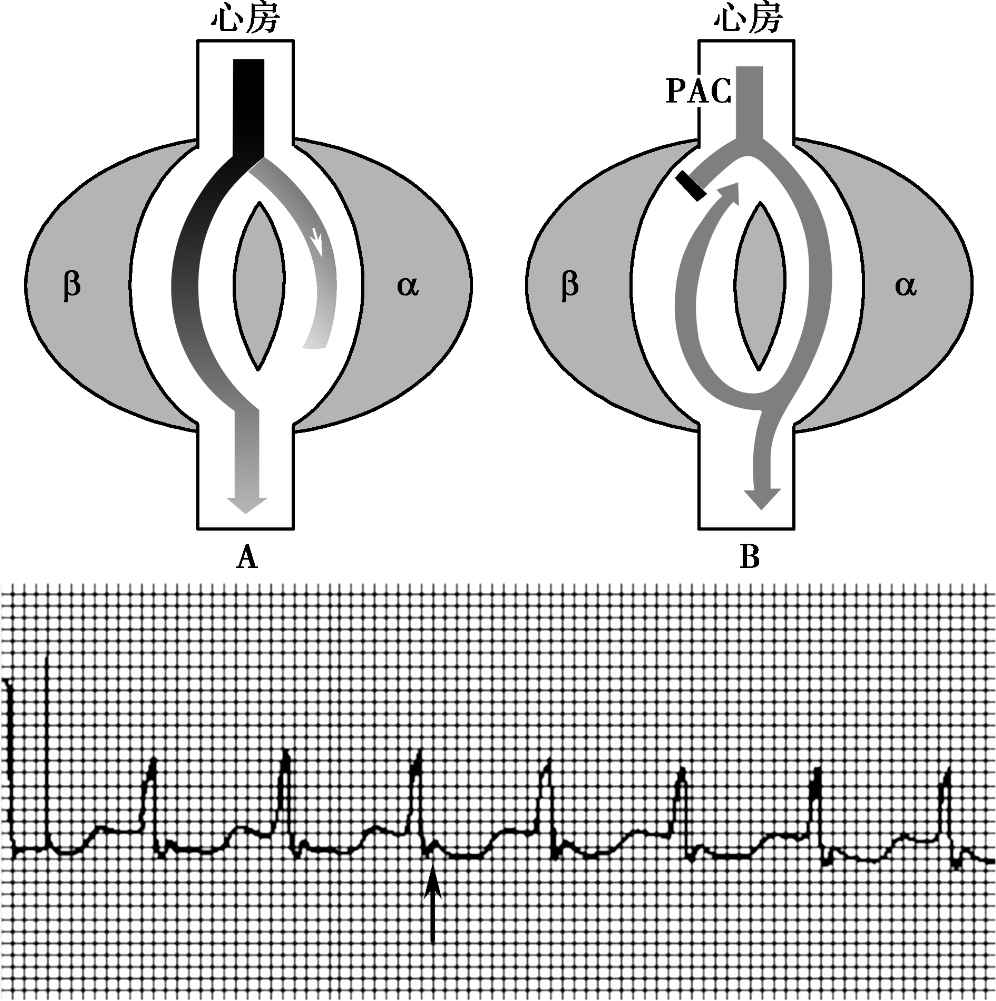
\includegraphics[width=3.14583in,height=3.16667in]{./images/Image00412.jpg}
 \captionsetup{justification=centering}
 \caption{示房室结折返性心动过速(慢-快型)的机制(↑示逆行P波)}
 \label{fig102-1}
  \end{figure} 



AVNRT根据其传导特点及电生理特征,分为以下三型:

\paragraph{慢 -快(S-F)型}

折返途径以慢通道前传,快通道逆传,占AVNRT的90\%。其电生理特征有:①心动过速易为电生理检查诱发或终止。②心房程序刺激时房室传导时间跳跃延长,当S\textsubscript{1}
S\textsubscript{2} 缩短10ms,跳跃值>
50ms,房室结反应曲线呈典型不连续性。③VA完全融合或紧随心室激动后发生(V-A
<
50ms)。④逆传高位右房、希氏束和冠状窦A波激动于同一条垂直线上或希氏束的A波略提前(中心性逆传),少数情况冠状窦近端A波稍提前。心动过速时为长A-H间期,A-H/H-A
>
1。⑤若典型AVNRT者,房性期前收缩刺激不能显示顺向性双径路反应,则提示双通道的不应期相似。心动过速伴束支阻滞不影响H-A间期或心动过速频率。

\paragraph{快-慢(F-S)型}

快(β)径路前传,慢(α)径路逆传,占AVNRT的5\%左右。其电生理特征有:①极易为电生理检查诱发或终止,常为持续性。②心动过速时无A-H延长,A-H/H-A
< 1。③最早心房逆传在冠状窦口附近。④无典型A-H间期的跳跃延长。

\paragraph{慢-慢(S-S)型}

多为房室结内多通道传导所致,激动前传或逆传均经慢径路。其电生理特征有:①心动过速时V-A无融合,V-A间期多>
120ms,但< 1/2 R-R间期。②A波逆传顺序不变,并处于同一垂直时限上。

\hypertarget{text00289.htmlux5cux23CHP10-2-2-1-1-4}{}
(四) 房室折返性心动过速

房室折返性心动过速(atrial ventricular reentrant
tachycardia,AVRT)占SVT的10\%~30\%左右。详见本章第7节“预激综合征伴快速性心律失常”。

\subsubsection{自律性增高性室上性心动过速}

在某些病理生理状态下(内源性或外源性儿茶酚胺增多、电解质紊乱、心肌缺血、机械性效应、药物毒性作用等),均可使潜在的起搏点自律性增高,或静息膜部分除极化引起自律性异常而导致快速性室上性心律失常。此类SVT的电生理特征为:①不为程序刺激诱发或终止。②不为超速起搏所终止。③无超速加速现象。④期前刺激周期与回响周期无相关。⑤心室晚电位阴性。⑥维拉帕米无明显疗效。

\hypertarget{text00289.htmlux5cux23CHP10-2-2-1-2-1}{}
(一) 自律性房性心动过速

自律性房性心动过速(automatic atrial
tachycardia,AAT)占SVT的4\%左右。洋地黄中毒为其主要病因,亦常见于急性心肌梗死、急性感染、酗酒、低钾或低氧血症、严重肺心病等,少见于无器质性心脏病的儿童,成年后自行消失。

心房肌病变使快反应电位转为慢反应电位,心房肌细胞舒张期自动除极速度加快,病变心房肌部分除极和(或)舒张期震荡电位致心房内异位兴奋灶自律性中度增高,发放激动频率加快。其电生理特征有:①心动过速开始时P波频率逐渐加快,不能为心房刺激诱发和终止,且发作与终止不依赖于房内和房室结传导迟缓。②房室结传导阻滞不影响心动过速的存在。③通常(并不总是)为超速起搏所抑制。④心房激动顺序取决于自律性增强点的位置,而不同于窦性心律。⑤兴奋迷走神经虽不能终止心动过速,但可能产生房室传导阻滞。

\hypertarget{text00289.htmlux5cux23CHP10-2-2-1-2-2}{}
(二) 非阵发性交界性心动过速

非阵发性交界性心动过速(non-paroxysmal junction
tachycardia,NPJT)为一类由于交界区内激动形成异常或传导功能异常所致短阵发作的心律失常。机制与房室交界区起搏细胞4相上升速度中度增加有关。常见于洋地黄中毒、心肌梗死、心肌炎及心脏手术后,偶见于健康年轻人。常为暂时性,可自行终止。

\subsubsection{触发激动性室上性心动过速}

局部儿茶酚胺水平增高、低血钾、高血钙及洋地黄中毒等,可引起细胞内钙积累,产生动作电位后的除极化,当期后除极振幅增高达阈电位水平,可致重复激动。

触发活动所致室上速的共同电生理特点为:①可由房性期前收缩及心房起搏所诱发,且不依赖于房内传导延缓和房室结传导延缓。②期前刺激周期与回响周期呈正相关。③存在超速加速现象。④自发终止前常表现为心率下降。⑤心室晚电位阴性。⑥兴奋迷走神经可以或不可以终止心动过速。⑦维拉帕米治疗有效。

\hypertarget{text00289.htmlux5cux23CHP10-2-2-1-3-1}{}
(一) 房性心动过速伴房室阻滞

房性心动过速伴房室阻滞(paroxysmal atrial tachycardia
block,PATB)可持续或间歇存在,房速时的短P′-P′间期,使P′容易出现在收缩期或舒张早期而发生干扰性房室传导障碍,因存在房室传导阻滞而常可排除折返所致室上速。病因多为洋地黄过量(伴低钾)所致,亦可与洋地黄应用无关;发生于器质性心脏病者常需停用洋地黄,而发生在健康者则常需应用洋地黄。

\hypertarget{text00289.htmlux5cux23CHP10-2-2-1-3-2}{}
(二) 多源性房性心动过速

多源性房性心动过速(multi-focal atrial
tachycardia,MAT)又称紊乱性房性心动过速(chaotic atrial
tachycardia,CAT)。曾认为其发生与心房内多个异位起搏点自律性增高或多发性房内折返有关,现认为由于心房壁损伤及张力增大,心动过速时伴有血浆儿茶酚胺增多,因触发激动引起心房内多个异位激动所致的房性心动过速。多见于50岁以上者,最常见于慢性肺心病、冠心病及糖尿病患者,亦与洋地黄过量、低钾、低镁等有关。

\subsection{诊断}

\subsubsection{临床表现特点}

心动过速的起始和终止常较突然,其诱发因素多为情绪激动、体位突然改变、猛然用力或饱餐,有时并无明显诱因。发作时症状与心动过速所致血流动力学功能障碍程度密切相关,而后者又受患者年龄、有无器质性心脏病基础、基础心功能状态、心动过速频率以及重要器官基础血供状态等因素影响。发作在无器质性心脏病的年轻患者,频率<
200次/分,且持续时间较短的,大多仅有突然心悸感,有时伴恐惧、不安和多尿,在有器质性心脏病基础的患者,频率>
200次/分,且持续时间较久的,可引起心脑等器官供血不足,导致血压下降、头晕、黑矇、心绞痛、心力衰竭等。脉搏细弱,听诊可闻快速、规则而匀整的心律,颈静脉搏动与心率一致。

\subsubsection{心电图特征}

一系列快速、规则的QRS波群,频率大多160~220
次/分,平均200次/分左右。QRS波群大多不增宽畸形,保持窦律时形态,ST段压低和T波倒置常见;但若伴有束支传导阻滞、室内差异传导或预激综合征时则QRS波可增宽变形。P波多重合于QRS波群内而看不到(AVNRT);若能看到时,则多为逆行P波,P′R/RP′
> 1(AVNRT或AVRT);少数P波为非逆行性,P′-R≥0.12秒,P′R/RP′ <
1,P波形态可与窦性P波相同(SANRT),也可与窦性P波不同(IART或AAT)。不同类型的SVT,其心电图表现亦有所差异:

\hypertarget{text00289.htmlux5cux23CHP10-2-2-2-2-1}{}
(一) SANRT

ECG特征为:①由连续3个以上节律规整的窦性P波组成,频率100~150次/分,常呈短阵发作。②P波在QRS波前,P-R
<
R-P间期,P-R间期长短与SVT的频率相关。③心动过速的P波形态和电轴与窦律时一致,P-P间期规则或略不规则。④可因房性期前收缩或窦性节律加速而诱发;可为房性期前收缩所终止,可伴散发窦性期前收缩。发作终止前P-P间期逐渐延长或长短交替性改变,发作后间歇呈等周期代偿。

\hypertarget{text00289.htmlux5cux23CHP10-2-2-2-2-2}{}
(二) IART

ECG特征为:①心动过速时P′形态、幅度、方向及时间不同于窦性P波,频率100~150次/分(少数达250次/分),P′-P′间期匀齐。②P′波位于QRS波群前,P′-R间期多>
0.12秒;P′-R间期< 1/2 R-R,R-P′间期> 1/2
R-R。③可由房早诱发,刺激迷走神经虽减慢心室率但不能使之终止;房早或反复搏动可终止发作。④可伴不同程度房室干扰、隐匿性传导、时相性室内差异性传导及束支蝉联现象。心动过速起始无P′波频率逐渐加快现象。

\hypertarget{text00289.htmlux5cux23CHP10-2-2-2-2-3}{}
(三) AVNRT

\paragraph{慢 -快型}

心电图特征为:①常由房性期前收缩或交界性期前收缩诱发,诱发的室上性期前收缩P-R间期较正常窦律时显著延长;由室性期前收缩诱发者,R-P′间期短,P′-R间期长。②心室率多为160~240次/分,R-R间期匀齐,QRS波群形态正常,少数伴差异性传导。③逆行P′波多隐藏于QRS波群中,少数病例P′波在Ⅱ、Ⅲ、aVF导联QRS终末部分(“假性S波”);V\textsubscript{1}
导联为假性r′波(图\ref{fig102-2})。④R-P′ > P′-R,R-P′ < 1/2 R-R,R-P′间期<
0.08秒。⑤刺激迷走神经可终止心动过速。

\paragraph{快 -慢型}

心电图特征为:①心动过速的发作无P-R间期延长,不需期前收缩诱发,只需心率稍增即可诱发,且常为持续性,心率约100~150次/分,律绝对规则。②逆行P′波于Ⅱ、Ⅲ、aVF导联倒置。③逆行P′波位于QRS波前,R-P′间期>
P′-R间期,R-P′ > 1/2
R-R。④QRS波群为宽大畸形或时限正常。⑤刺激迷走神经可终止室上速。

\hypertarget{text00289.htmlux5cux23CHP10-2-2-2-2-4}{}
(四) AVRT

其心电图特征详见本章第7节“预激综合征伴快速性心律失常”。

\hypertarget{text00289.htmlux5cux23CHP10-2-2-2-2-5}{}
(五) AAT

ECG特征有:①心率150~250次/分,P′-P′间期常不很规则。②QRS波呈室上性,P′波异于窦性P波而与房性期前收缩P′波相同,P′波位于QRS波前,P′-R间期<
R-P′间期,P′-R间期长短与心动过速的频率有关。③发作起始时频率逐渐加速,终止前逐渐减速(“温醒现象”)。④心动过速发作时可伴有房室或束支传导阻滞。⑤刺激迷走神经常不能使心动过速终止。

\hypertarget{text00289.htmlux5cux23CHP10-2-2-2-2-6}{}
(六) NPJT

ECG特征有:①心室率70~130次/分。②逆行P波位于交界性QRS波群前或后,室房分离,室率快于房率,可见各种房性融合波。③心动过速起始频率逐渐加快。④心动过速发作前后常见单个或成对交界性期前收缩。⑤窦律与NPJT并存,心室激动受窦房结或交界区心律的交替控制。

\hypertarget{text00289.htmlux5cux23CHP10-2-2-2-2-7}{}
(七) PATB

ECG特征有:①心房节律规则,心室节律可规则或不规则。②心房率150~250次/分,心室率依阻滞比例而定。③P′波位于QRS波前,QRS波呈室上性,P′-R
<
R-P′间期。④传导阻滞可为一度、文氏型或莫氏型、高度或完全性(图\ref{fig102-3})。⑤洋地黄中毒所致者还可伴有单源或多源室性期前收缩。

\hypertarget{text00289.htmlux5cux23CHP10-2-2-2-2-8}{}
(八) MAT

ECG特征有:①一系列三种以上形态的P′波,但无一种波形为主,频率快慢不一,100~250次/分。②P′-R间期或R-R间期和(或)P′-P′间期长短不一,但均>
0.12秒;P′-P′之间存在等电位线;P′波位于QRS波前,P′-R <
R-P′间期;心室率100~250次/分;伴有房室传导阻滞时室律可不规则。③发作可持续数分钟至数日,甚至数月不等。可蜕变为房颤或房扑,可在同一导联上房性期前收缩、紊乱性房性心动过速和房颤交替出现(图\ref{fig102-4})。

几种常见的阵发性SVT的ECG鉴别诊断见表\ref{tab102-1}。

窄QRS波心动过速的心电图鉴别诊断程序及对腺苷反应的诊断程序,颇具临床实用价值。详见图\ref{fig102-5}、图\ref{fig102-6},有关宽QRS波心动过速的诊断程序见本章第8节“宽QRS心动过速”。

\subsubsection{心电生理检查}

\begin{figure}[!htbp]
 \centering
 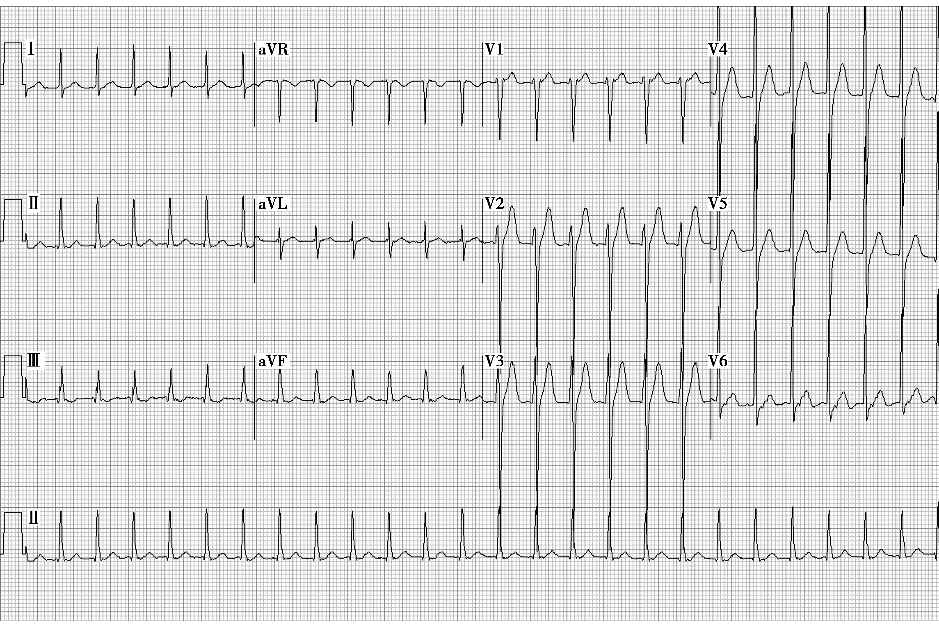
\includegraphics[width=6.29167in,height=4.19792in]{./images/Image00413.jpg}
 \captionsetup{justification=centering}
 \caption{房室结折返性心动过速(慢-快型)}
 \label{fig102-2}
  \end{figure} 

频率150次/分,V\textsubscript{6}
导联ST段起始部可见逆行P波,Ⅱ、Ⅲ、aVF可见假性S波,aVR可见假性r波

\begin{figure}[!htbp]
 \centering
 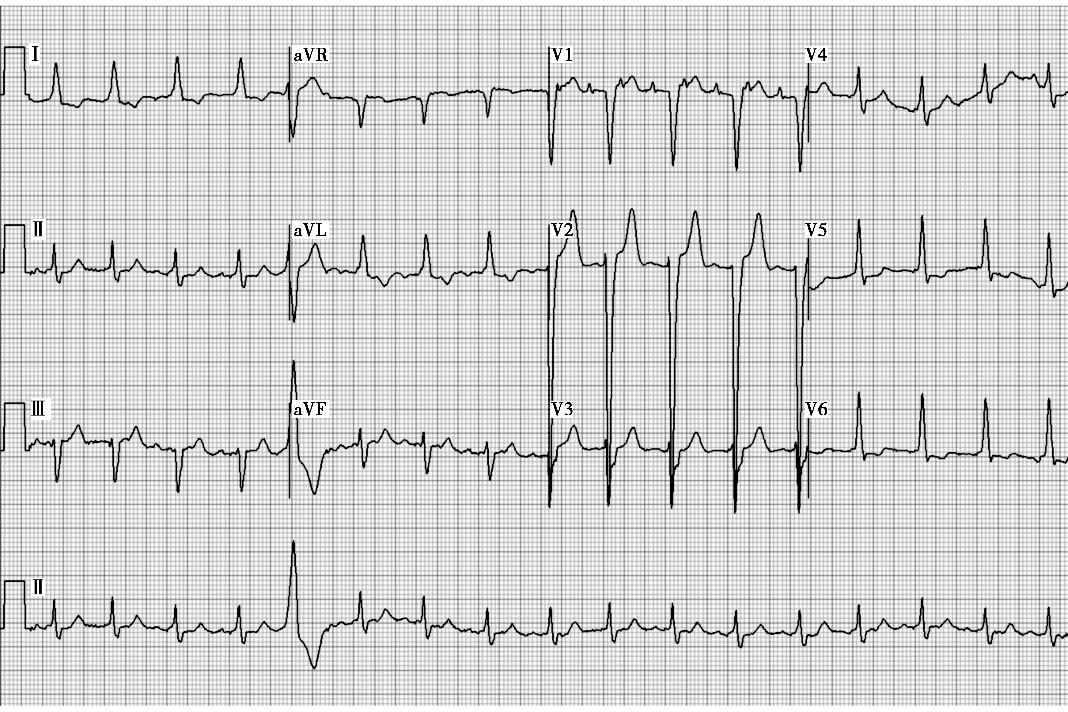
\includegraphics[width=6.29167in,height=4.19792in]{./images/Image00414.jpg}
 \captionsetup{justification=centering}
 \caption{示阵发性房性心动过速伴2∶1房室传导阻滞}
 \label{fig102-3}
  \end{figure} 

心电生理检查对诊治室上速有重要作用,其适应证为:①有症状而诊断不明确者;②宽大QRS波群,不能鉴别室性或室上性者;③原因不明的晕厥或有猝死史;④需要在较短时间内选择有效抗心律失常药物;⑤明确定位,准备手术或消融治疗;⑥检验治疗效果。

\begin{figure}[!htbp]
 \centering
 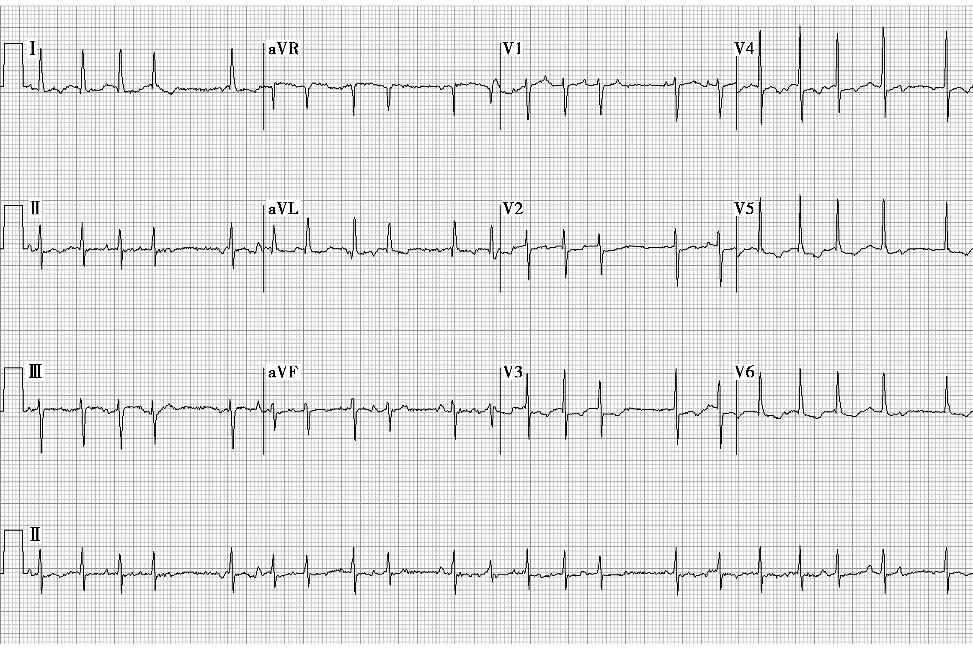
\includegraphics[width=6.29167in,height=4.19792in]{./images/Image00415.jpg}
 \captionsetup{justification=centering}
 \caption{多源性房性心动过速}
 \label{fig102-4}
  \end{figure} 

可见3种以上形态的异位P波,P波变化不呈渐进性,可与房内游走心律鉴别

\begin{table}[htbp]
\centering
\caption{常见室上速的鉴别诊断}
\label{tab102-1}
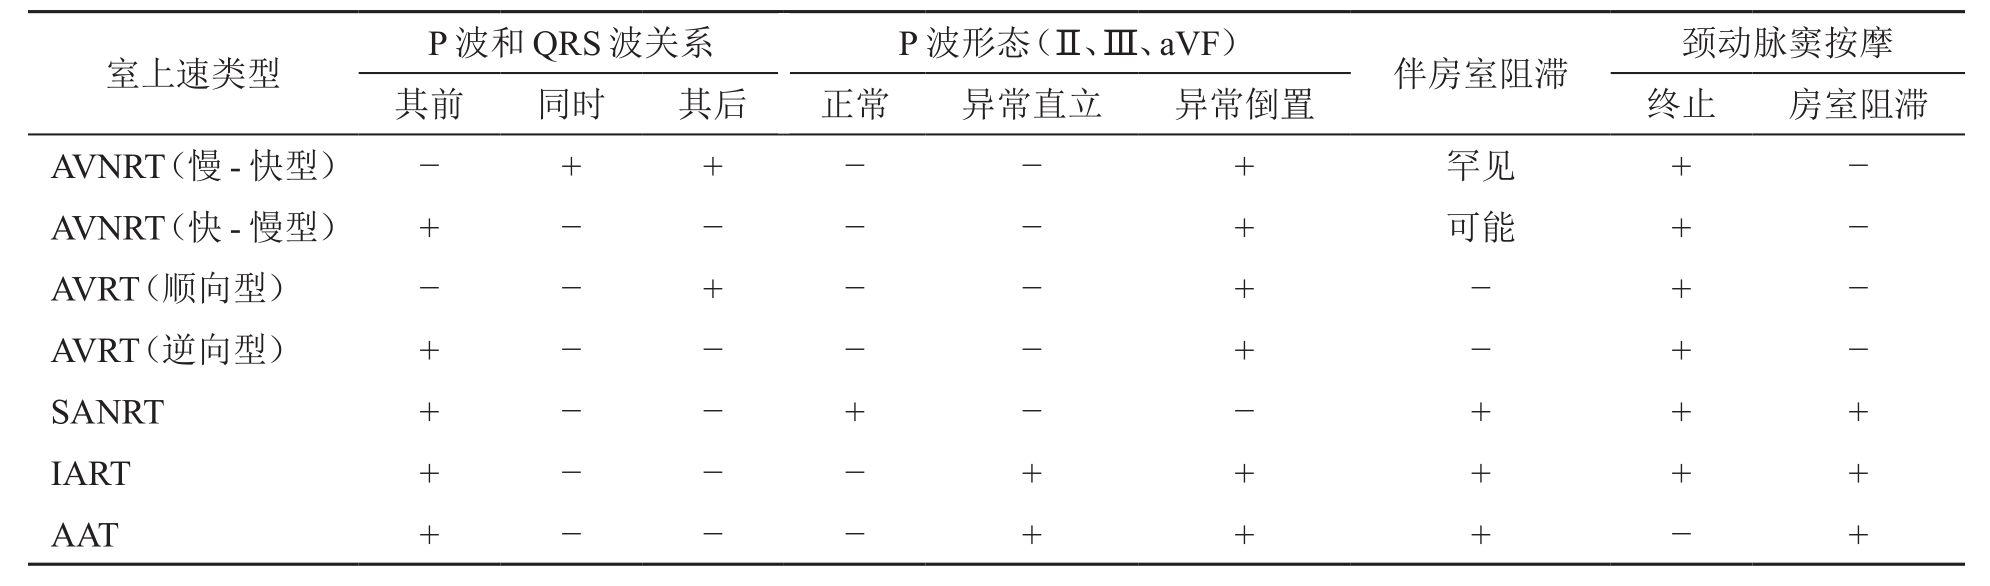
\includegraphics[width=6.625in,height=1.94792in]{./images/Image00416.jpg}
\end{table}

\paragraph{心内电生理检查}

有完整的调搏和记录方案。优点是能了解心内电图(希氏束电图、心房各部位电图等),精确地确定室上速的性质、旁路的部位及各部分的电生理参数。心内检查是进行非药物治疗前的必须步骤。

\paragraph{食管电生理检查}

可间接调搏左心房,记录食管内电图,诱发或终止室上速,对室上速的性质做出初选,并可观察药物的疗效。操作简便,易被接受,也较安全,是我国目前宜于推广的检查方法。

\subsection{治疗}

治疗首先针对基本心脏病,纠正重要诱发因素如低血钾、缺氧、感染等,停用诱发或可疑诱发的药物。对不同类型室上速的治疗分述如下:

\subsubsection{折返性室上性心动过速}

此类室上速为最常见的阵发性SVT,其中又以AVNRT最多见。

\hypertarget{text00289.htmlux5cux23CHP10-2-2-3-1-1}{}
(一) 急性发作期

应根据患者基础的心脏状况
,既往发作的情况以及对心动过速的耐受程度作出适当处理。

\paragraph{刺激迷走神经的物理方法}

如患者心功能与血压正常,可先尝试。常用物理方法有:①咽反射:以压舌板刺激咽部,诱发恶心呕吐;②Valsalva动作(深吸气后闭住口鼻用力作呼气动作)或Müller动作(深呼气后闭住口鼻再用力作吸气动作);③压迫眼球法:患者平卧位,闭目下视,用拇指在一侧眶下适度压迫眼球上部,以刺激球后副交感神经末梢,持续时间约10秒。先压右眼,后压左眼(不能两眼同时压迫),如此操作2~3次,无效者停止压迫。此法常致患者眼球疼痛,甚至招致视网膜剥离。青光眼、高度近视或已有视网膜病变者禁用,老年人不宜用;④颈动脉窦按摩法:患者取仰卧位,在下颌骨角下相当甲状软骨上缘的水平,摸到颈动脉分叉处的搏动,用手指将颈动脉向颈椎横突方向加压并按摩,先右后左,每次约10秒,切忌同时两侧按摩。有颈动脉血管杂音或病变或颈动脉窦过敏、脑供血不足及老年人禁用。⑤冷水面部浸浴(潜水反射):患者深吸气后屏气,将面部浸入2~10℃冷水盆内20~40秒,心动过速可在5~35秒内转复。本法可致全身血管张力升高,AMI、高血压者应避免使用;SSS与AVB者也不宜用。

\begin{figure}[!htbp]
 \centering
 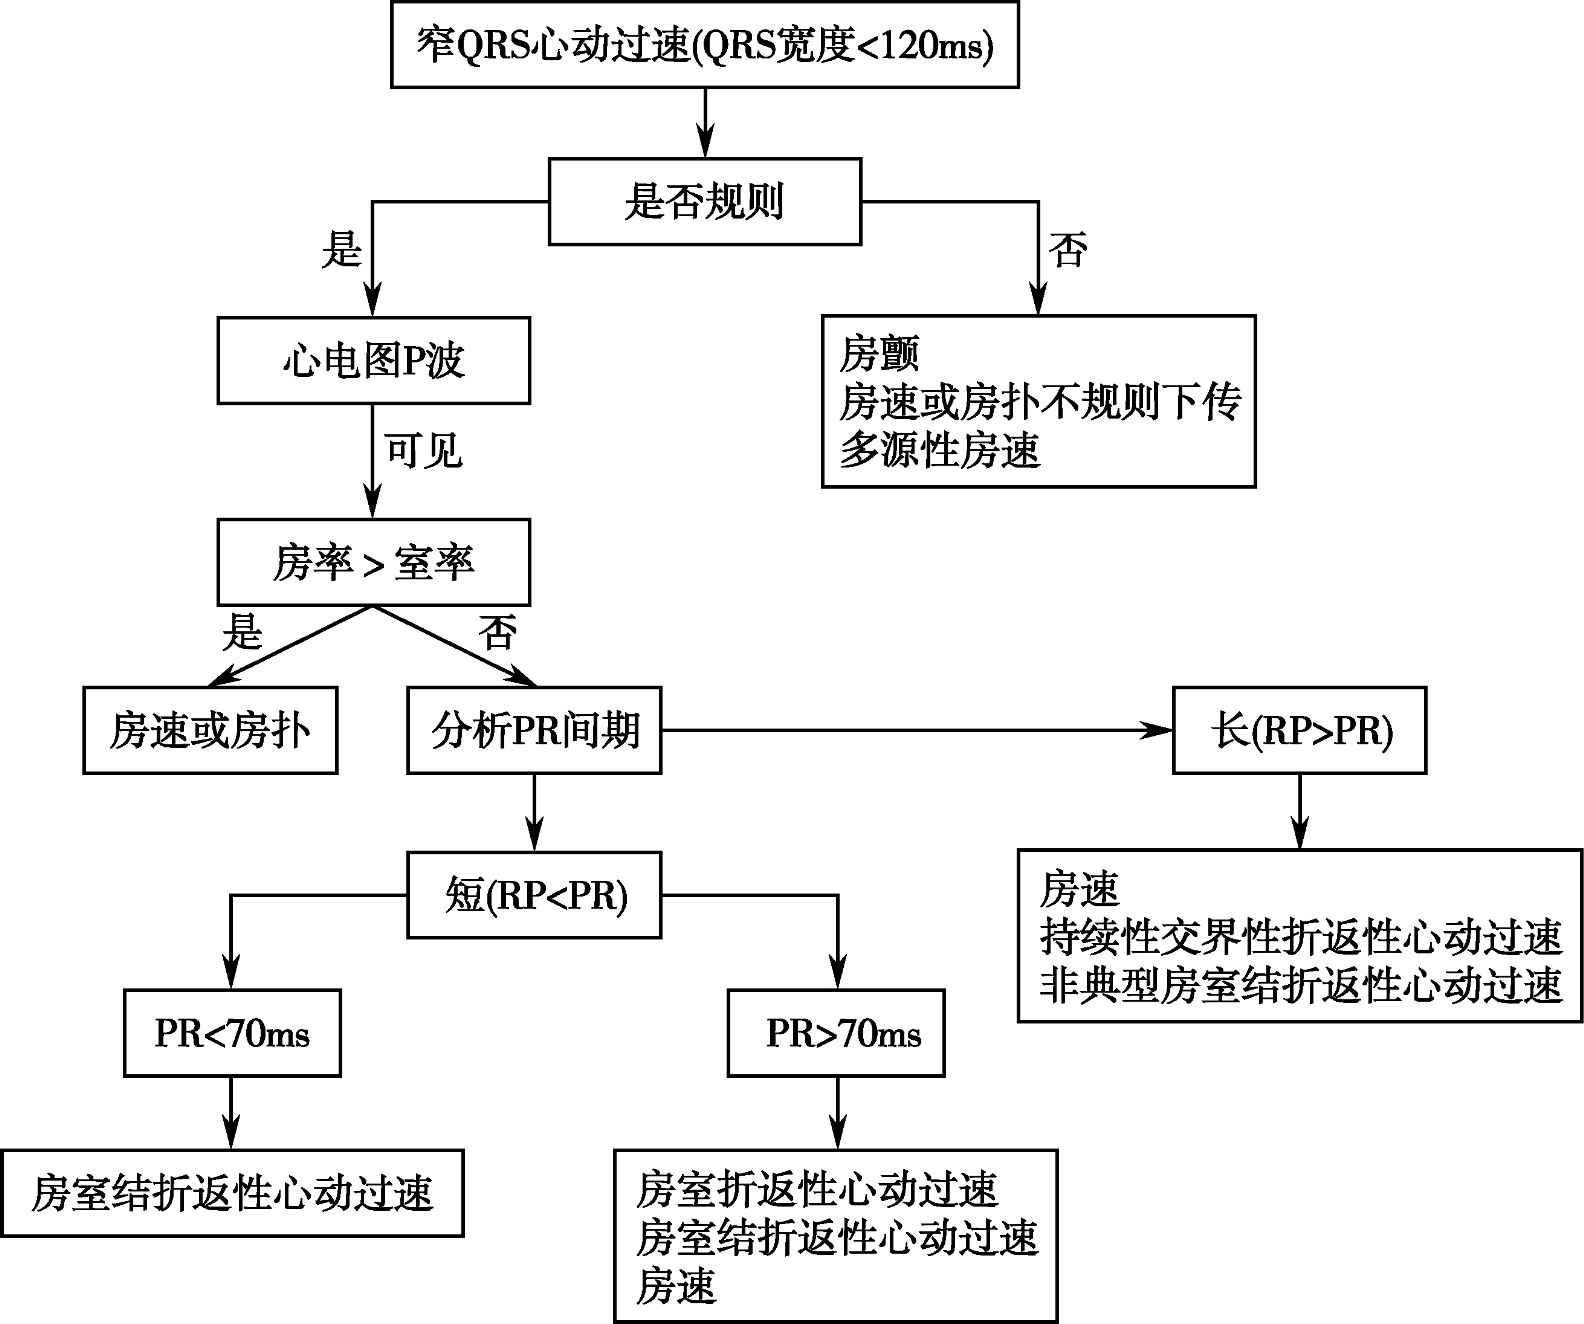
\includegraphics[width=4.36458in,height=3.64583in]{./images/Image00417.jpg}
 \captionsetup{justification=centering}
 \caption{窄 QRS波心动过速的鉴别诊断程序}
 \label{fig102-5}
  \end{figure} 

\begin{figure}[!htbp]
 \centering
 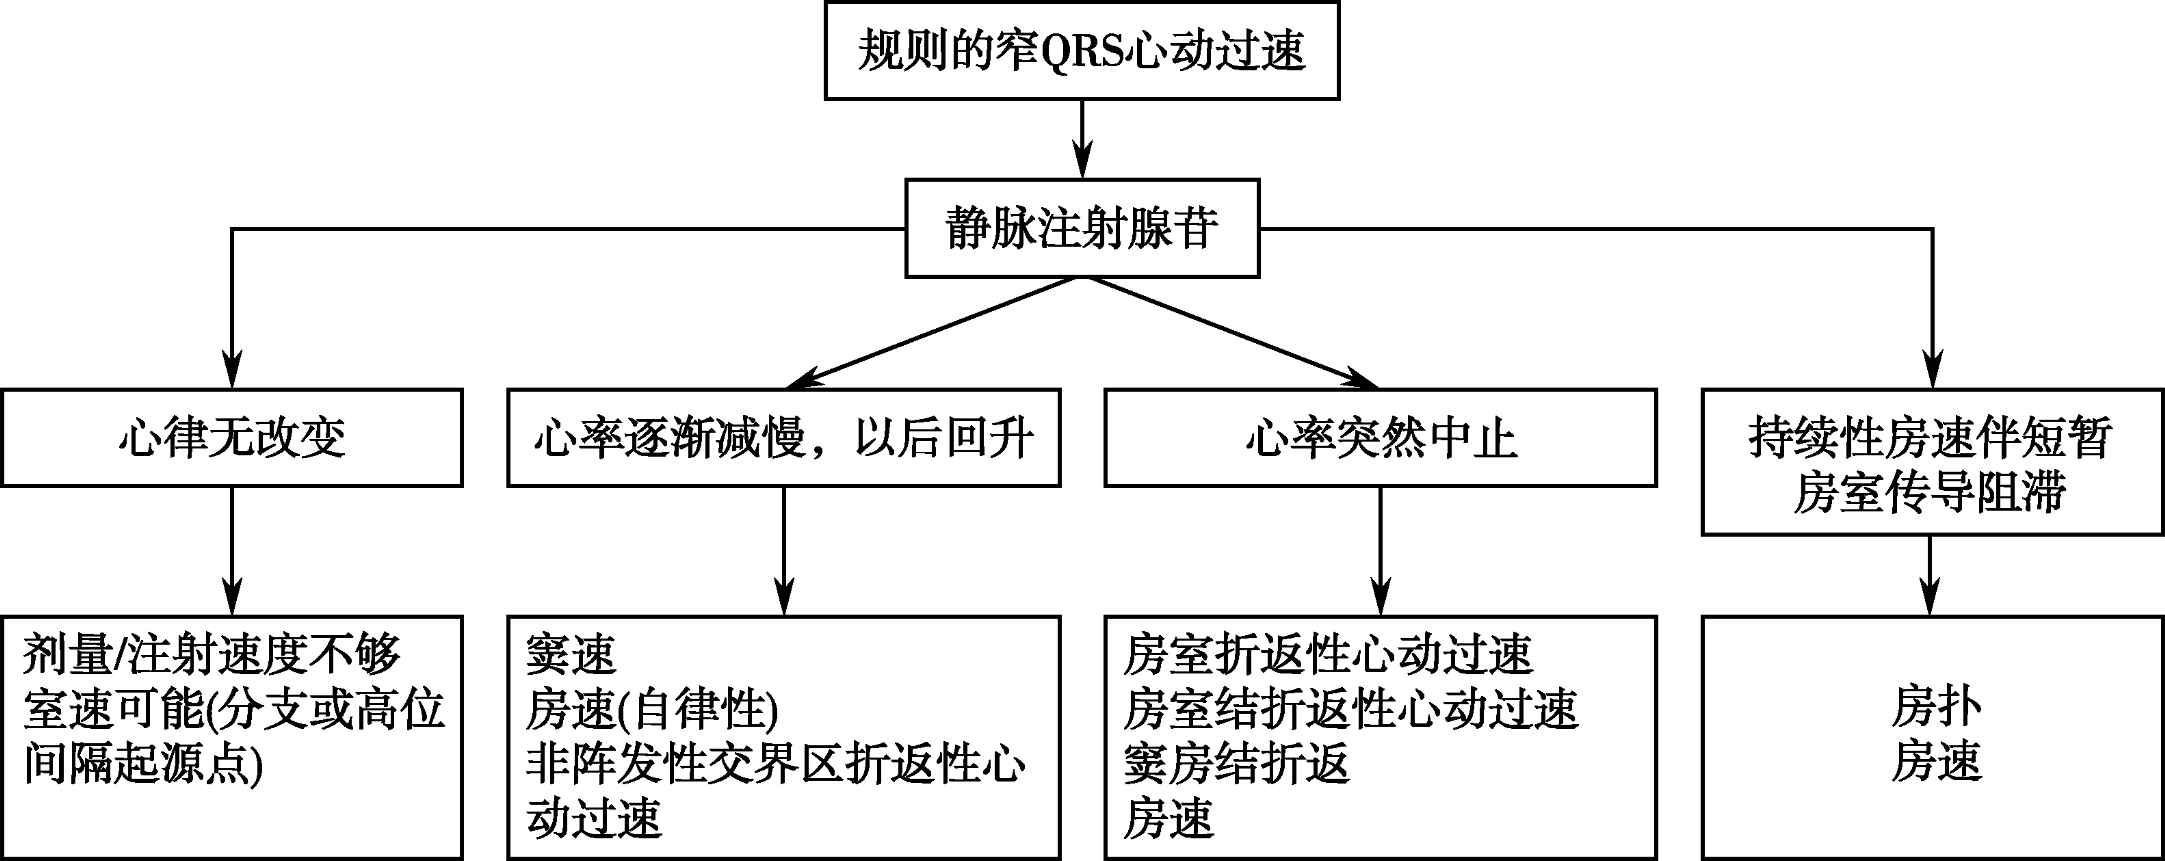
\includegraphics[width=5.27083in,height=2.09375in]{./images/Image00418.jpg}
 \captionsetup{justification=centering}
 \caption{窄 QRS波心动过速对腺苷反应的诊断程序}
 \label{fig102-6}
  \end{figure} 

\paragraph{腺苷}

为首选药物。心力衰竭、低血压和新生儿均可应用。常用6~12mg直接快速静注,5~10秒内注射完毕,3~5分钟后未复律者可重复1次。起效迅速,副作用为胸部压迫感、呼吸困难、面部潮红和严重窦性心动过缓、窦性停搏、房室传导阻滞、室性心律失常等瞬间心律失常等。因其半衰期短于6秒,副作用即使发生亦很快消失。合并心绞痛、支气管哮喘、室性心律失常、SSS及年龄>
60岁者应慎用或禁用。

\paragraph{维拉帕米}

对正常QRS波群的PSVT效果好,转复成功率高达90\%~100\%,曾被认为是治疗室上速的首选药物。静注后1~5分钟起效,10分钟作用达高峰,持续15分钟以上。用法:5mg稀释于25\%葡萄糖液20ml中静注,5分钟推完;15分钟后仍未能转复者可重复1次。一般总量不超过15mg为安全。应用时注意:①严禁在短时间内与β阻滞剂联合用药以免造成严重AVB;②因对窦房结的自律性有轻度抑制作用,SSS者应慎用或禁用;③静注剂量过大或速度过快时可引起AVB、血压降低,甚至心脏骤停等严重后果,一旦发生可静注阿托品、静滴异丙肾上腺素以及10\%葡萄糖酸钙10ml静注,严重AVB者,可用心室临时起搏;④心动过缓、低血压、心功能不全、AVB者禁用。

\paragraph{毛花苷丙(西地兰)}

起效缓慢,一般复律时间需30分钟以上,但作用温和,是PSVT合并心力衰竭的首选药物。用法:如两周内未用过洋地黄制剂可用0.4~0.8mg加入10\%~25\%葡萄糖液20~40ml中缓慢静注;1~2小时后无效可再给0.2~0.4mg,总量不超过1.2mg。WPW伴逆向型AVRT患者禁用。

\paragraph{β受体阻滞剂}

伴有高血压或心绞痛的PSVT患者宜首选β受体阻滞剂。常用艾司洛尔50~200μg/kg静注,亦可用普萘洛尔(2~5mg静注,必要时20~30分钟后可重复1次)、美托洛尔等静注。失代偿的心力衰竭、支气管哮喘等患者禁用。

\paragraph{普罗帕酮}

用法:1~1.5mg/(kg•次)(常用70mg)加入25\%葡萄糖液20~40ml中静注,10~20分钟后无效重复1次,一般静注总量不超过210mg。由于普罗帕酮有负性肌力作用及抑制传导系统作用,且个体间存在较大差异,对有心功能不全者应禁用,对有器质性心脏病、低血压、休克、心动过缓者等慎用或禁用。

\paragraph{升压药物}

合并低血压者可应用升压药物如去氧肾上腺素(5~10mg/次)、甲氧明或间羟胺等,但老年患者高血压AMI等禁用。

其他可供选用的药物有胺碘酮、奎尼丁等。

\paragraph{特殊情况下药物选择}

①伴有COPD者,可用钙拮抗剂维拉帕米或地尔硫{}
,禁用腺苷、ATP等。②SSS合并PSVT,应先置入临时心室起搏电极,再静脉用药,以策安全。③孕妇合并PSVT,选用刺激迷走神经的物理方法或食管调搏复律;药物首选毛花苷丙,次选维拉帕米或普罗帕酮。

\paragraph{食管心房调搏复律}

对终止PSVT是一种简单易行且有效的治疗方法。对药物无效或暂不能用药物治疗者,可选用。

\paragraph{直流电复律}

伴严重血流动力学障碍(心绞痛、低血压、心力衰竭)的PSVT患者,应首选同步直流电复律;急性发作以上治疗无效者,也应使用。但已应用洋地黄者不应行直流电复律治疗。

\hypertarget{text00289.htmlux5cux23CHP10-2-2-3-1-2}{}
(二) 预防复发

是否需要给予患者长期药物预防
,取决于发作频繁以及发作的严重性。症状不严重且无器质性心脏病的患者,以及偶然发作的患者无需长期服药预防。药物选择可依据临床经验或心内电生理试验结果,洋地黄制剂(地高辛0.125~0.25mg/d)、长效CCB(缓释维拉帕米240mg/d,长效地尔硫{}
60~120mg每日2次)或β受体阻滞剂(美托洛尔50~100mg/d)可供首先选用。也可用普罗帕酮0.1~0.2g,每日3~4次口服。射频消融疗法可根治AVRT和
AVNRT,是目前根治PSVT发作的主要手段,其成功率可达96\%~99\%。并发症少,安全,复发率低(<
3\%)。应优先考虑使用。

\subsubsection{其他类型室上速的治疗}

\paragraph{SANRT}

本型SVT心电图上难以与窦性心动过速鉴别,只是发作形式有所不同:SANRT常突发、突止,发作持续时间短,心动过速终止前出现心动周期延长;而刺激迷走神经方法仅能使窦性心动过速频率轻微减慢,不能使其突然终止。因发作时心率通常较慢(一般为150次/分左右),且持续时间短暂,无症状者可不需治疗;发作频繁者可用维拉帕米、普萘洛尔、洋地黄等治疗,并预防其复发。

\paragraph{IART}

刺激迷走神经不能终止发作,但可加重房室传导阻滞使心室率减慢。Ⅰa类药物疗效不佳,Ⅰc类药物有一定疗效,Ⅲ类药物疗效较满意;普萘洛尔、维拉帕米仅能降低心室率。心房调搏超速抑制可终止心动过速。

\paragraph{AVRT}

参见本章第7节“预激综合征伴快速性心律失常”。

\paragraph{AAT}

Ⅰa类药物有不同疗效;洋地黄中毒者停用洋地黄后,口服或静滴氯化钾;亦可慎用Ⅰb类药物或普萘洛尔;心动过速顽固者应予直流电复律。

\paragraph{NPJT}

此类心动过速多为短阵发作,一般不需特殊处理。治疗基础心脏病心动过速可能自动终止;洋地黄中毒者停用洋地黄和补钾,可用苯妥英钠、普萘洛尔或利多卡因,电复律可能无效。

\paragraph{PATB}

洋地黄过量所致者,停用洋地黄并补钾;无效可以静注苯妥英钠(一次量<
250mg);维拉帕米可能有效,但其可提高血清地高辛浓度,应慎用。非洋地黄中毒引起的发作,可予以洋地黄,或试用胺碘酮、维拉帕米。Ⅰa类抗心律失常药物因其减慢房率并促进1∶1房室传导,应慎用。

\paragraph{MAT}

应先治疗基础疾病,控制诱发因素(感染、心衰等)及补钾。选择性β\textsubscript{1}
受体阻滞剂美托洛尔有良好疗效,口服25~50mg,每日2~3次;口服或静注维拉帕米有效;Ⅰa类、Ⅰb类抗心律失常药物或洋地黄疗效欠佳。

\hypertarget{text00289.htmlux5cux23CHP10-2-2-4}{}
参 考 文 献

1. Lee KW,Badhwar N,Scheinman MM. Supraventricular tachycardia---part
I. Curr Probl Cardiol,2008,33(9):467-546

2. Lee KW,Badhwar N,Scheinman MM. Supraventricular tachycardia---Part
II:history,presentation,mechanism,and treatment. Curr Probl
Cardiol,2008,33(10):557-662

3.
中华医学会心血管病分会,中国生物医学工程学会心脏起搏与电生理分会,中华心血管病杂志编辑委员会,等.室上性快速心律失常治疗指南.中华心血管病杂志,2005,33(1):2-15

4. 陈灏珠 ,林果为.实用内科学.第13版.北京:人民卫生出版社,2009:1400

5. 陆再英,钟南山.内科学.第7版.北京:人民卫生出版社,2008:198

\protect\hypertarget{text00290.html}{}{}

\section{心房扑动}

心房扑动(房扑,atrial
flutter,AFL)是一种快速而规则的房性异位心律,它引起快而协调的心房收缩,而以不同程度的房室传导比例传入心室。多为阵发性,常是窦性心律与心房颤动相互转变时的短暂现象。其发作大多持续数小时至数天,且容易在洋地黄的影响下或自动转成房颤。

\subsection{病因与发病机制}

房扑几乎均发生于器质性心脏病患者,主要见于慢性肺源性心脏病、二尖瓣及三尖瓣病变和任何原因引起的心房扩大,尤其是右心房扩大的疾病;也见于手术后的患者和先心病Ebstain畸形等。其病因与房颤基本相似(详见本章第4节“心房颤动”)。

人类心房扑动(房扑)的主要机制是右心房内的大折返。此与右房内结构(上下腔静脉开口、卵圆窝、冠状窦开口等)有关,三条结间束的纵形连接、传导汇聚至房室结,是产生环形运动的潜在解剖学基础,Koch三角后下部、下腔静脉开口、三尖瓣环及冠状窦口间的嵴部为房扑折返环最狭窄部位,该部位为传导缓慢区域,区域内可测得局部双电位和碎裂波。局部双电位的机制:①其代表功能性的折返环中心,记录到电极两侧先后通过折返环激动电位。②代表折返环内的缓慢传导区入口和出口电位。碎裂波为传导延缓的标志,亦为控制房扑周期长度、抗心律失常药物的作用点和射频消融的靶点图。

房扑发作时激动沿母环周而复始地连续环行折返,母环发出许多子波,以固定速度循固定途径传导。Ⅰ型房扑发作时激动呈逆钟向旋转的大折返,激动在右心房沿房间隔向上达右房上部,后经右房前侧壁向下激动,在Ⅱ、Ⅲ、AVF分别形成F波前半负向(房间隔除极)和后半正向(前侧壁激动);左房激动则是被动的。Ⅱ型房扑发病机制尚不明了,可能为右心房顺钟向旋转的折返环或左房内折返。

\subsection{诊断}

\subsubsection{临床表现特点}

\paragraph{症状}

临床上随心室率的快慢及原有心脏病的轻重不同,可有心慌、闷气、心绞痛、休克、心力衰竭、昏厥等表现。

\paragraph{体征}

房扑时心室律规则,140~160次/分左右,但当房室传导比例的固定性关系发生变化时,脉搏可变为不规则,与房颤相似,可出现脉搏短绌。有时由于房室传导比例改变,心室率可突然自动成倍增减。按摩颈动脉窦或压迫眼球可使心室率减慢或突然减半;解除压迫后又即回复到原有心率水平。仔细听诊心脏有时可听到心房收缩音;观察颈静脉可能看到心房收缩引起的频数静脉搏动,超过心搏率。

\subsubsection{心电图特征}

\hypertarget{text00290.htmlux5cux23CHP10-2-3-2-2-1}{}
(一) Ⅰ型房扑(亦称普通型,common type)

心电图特征有:①P波消失,代之以250~350次/分波形和振幅相同、间期匀齐的锯齿样心房扑动波(F波),其多呈三角形,波峰尖角或圆钝,其间无等电位线;Ⅱ、Ⅲ、AVF和V\textsubscript{6}
导联呈负向,V\textsubscript{1}
导联呈正向。②房室传导以2∶1为最常见形式,室律规则为150次/分左右,此时F波常重叠于T波上,锯齿状特征被掩盖,易误诊为室上速,必要时压迫颈动脉窦,加重房室传导阻滞使室率减慢,F波显现。若为1∶1传导常提示隐匿性房室传导,此时可致极快的心室率。还可有3∶1~6∶1或3∶2、4∶3、5∶4等不同传导比例(图\ref{fig102-7})。若传导比例恒定,则心室率是规则的,反之则显著的不齐。③F-R间期通常较窦律P-R间期长,F-R间期一般固定,若4∶1或6∶1传导时则可延长,若伴二度房室传导阻滞或交界区心动过速时,F-R间期可不规则。④R-R间期相等,但若隐匿性传导合并三度房室传导阻滞,可见短长心室周期交替出现。QRS波群和时限与窦性心律时相同,但若伴束支传导阻滞、时相性室内差异性传导、预激综合征时可宽大畸形。房扑与窦性心动过速的鉴别见表\ref{tab102-2}。

\begin{table}[htbp]
\centering
\caption{房扑与窦性心动过速的鉴别}
\label{tab102-2}
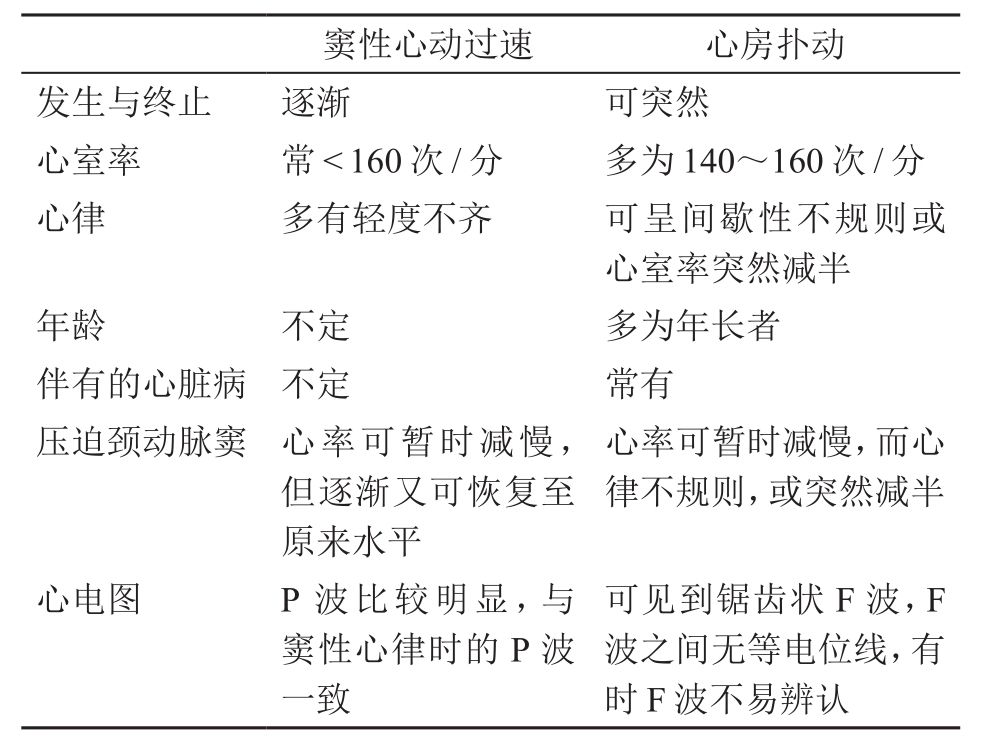
\includegraphics[width=3.32292in,height=2.46875in]{./images/Image00421.jpg}
\end{table}

\hypertarget{text00290.htmlux5cux23CHP10-2-3-2-2-2}{}
(二) Ⅱ型房扑(亦称非普通型,uncommon type)

F波频率340~430次/分,Ⅱ、Ⅲ、AVF导联F波正向,以直立圆凸较多,V\textsubscript{1}
导联F波负向;F波间无等电位线,振幅达0.3~0.6mV;同一患者,Ⅰ型和Ⅱ型房扑可交替出现。

\hypertarget{text00290.htmlux5cux23CHP10-2-3-2-2-3}{}
(三) 房扑合并其他心律失常

房扑合并的心律失常有
:伴二度和三度房室传导阻滞、束支及分支传导阻滞、时相性差异性传导、束支内蝉联现象、交界性或室性逸搏、交界性或室性逸搏心律、非阵发性交界性心动过速、室性期前收缩、室性心动过速等。

\hypertarget{text00290.htmlux5cux23CHP10-2-3-2-2-4}{}
(四) 房扑还可有以下特殊类型

1.不纯性房扑 以F波为主的房扑夹杂着少数f波者。

2.房扑房颤 F波与f波先后出现,持续时间大致相等者。

3.扭转型房扑 F波尖端围绕基线扭转,类似尖端扭转型室速者。

4.房扑伴局限性完全性心房内传导阻滞 心电图分别表现为F波和P波两组图形者。

5.应用Ⅰ类和Ⅲ类抗心律失常药物后,F波频率慢至160~200次/分,F波振幅达0.3mV左右。

6.房扑有时频率高达400次/分,F波振幅较小而F-F间存在等电位线。

7.房扑伴传出阻滞呈文氏现象时
,F-F周期逐渐缩短后F波漏搏,后又重复新的周期性变;若伴固定型传出阻滞,长F-F周期为基本F-F周期倍数。

\begin{figure}[!htbp]
 \centering
 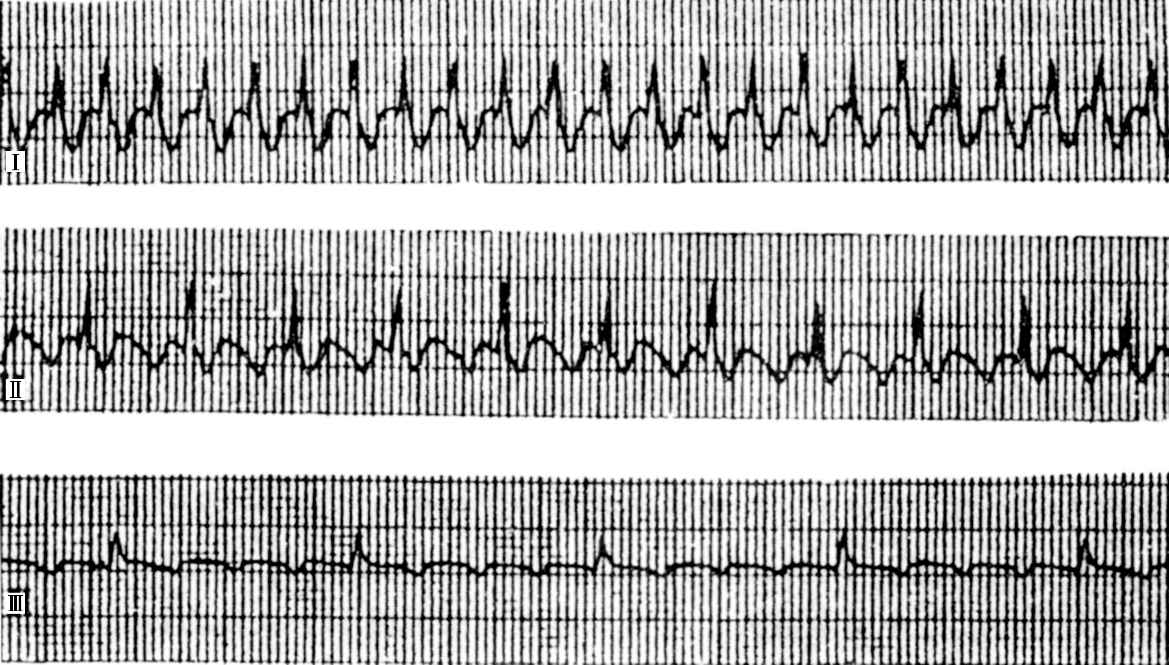
\includegraphics[width=6.29167in,height=3.58333in]{./images/Image00422.jpg}
 \captionsetup{justification=centering}
 \caption{心房扑动伴1∶1传导(上),2∶1传导(中)和4∶1传导(下)}
 \label{fig102-7}
  \end{figure} 

\subsubsection{房扑的电生理特点}

\paragraph{Ⅰ型房扑}

①右房内大折返环形运动的缓慢传导区是功能性的,呈频率依赖性。②存在显性和隐匿性拖带。③可为快速起搏所终止。④可记录最早局部兴奋电位,往往代表折返环的起始部位(缓慢传导区的出口电位)。⑤可记录到碎裂电位,持续80~130ms;Ⅱ、Ⅲ、AVF导联F波起始部分与之同时发生。⑥可于右心房后中隔和冠状窦口周围记录到局部双电位,波形特点为一个心动产生两个由等电间期分离的电位。

\begin{table}[htbp]
\centering
\caption{心房扑动与阵发性房性心动过速的鉴别}
\label{tab102-3}
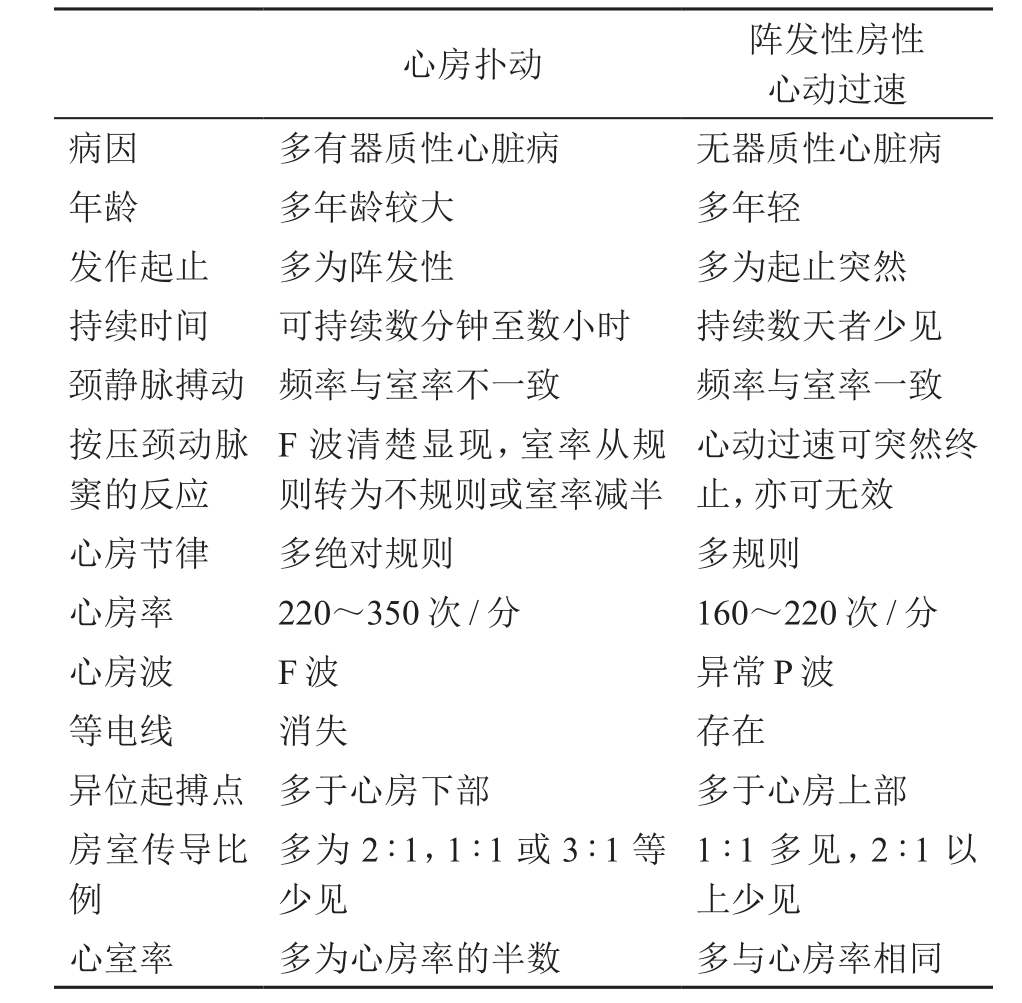
\includegraphics[width=3.39583in,height=3.33333in]{./images/Image00423.jpg}
\end{table}

\paragraph{Ⅱ型房扑}

房扑不受心房快速起搏的影响,快速高位心房起搏终止时Ⅱ型可转为Ⅰ型房扑。

\subsubsection{诊断注意事项}

由房性期前收缩诱发或由房性心动过速转变而来,亦可自行发作,心电图上快速绝对规则的锯齿状F波,心房率250~400次/分,不论心室节律是否匀齐,即可诊为心房扑动。但当房扑的房室传导比例为2∶1或1∶1时,应与阵发性房性心动过速相鉴别,见表\ref{tab102-3}。房扑2∶1下传伴完全性左束支阻滞时尚应与室性心动过速相鉴别,见表\ref{tab102-4}。

\begin{table}[htbp]
\centering
\caption{2∶1房扑伴完全性左束支阻滞与室性心动过速的鉴别}
\label{tab102-4}
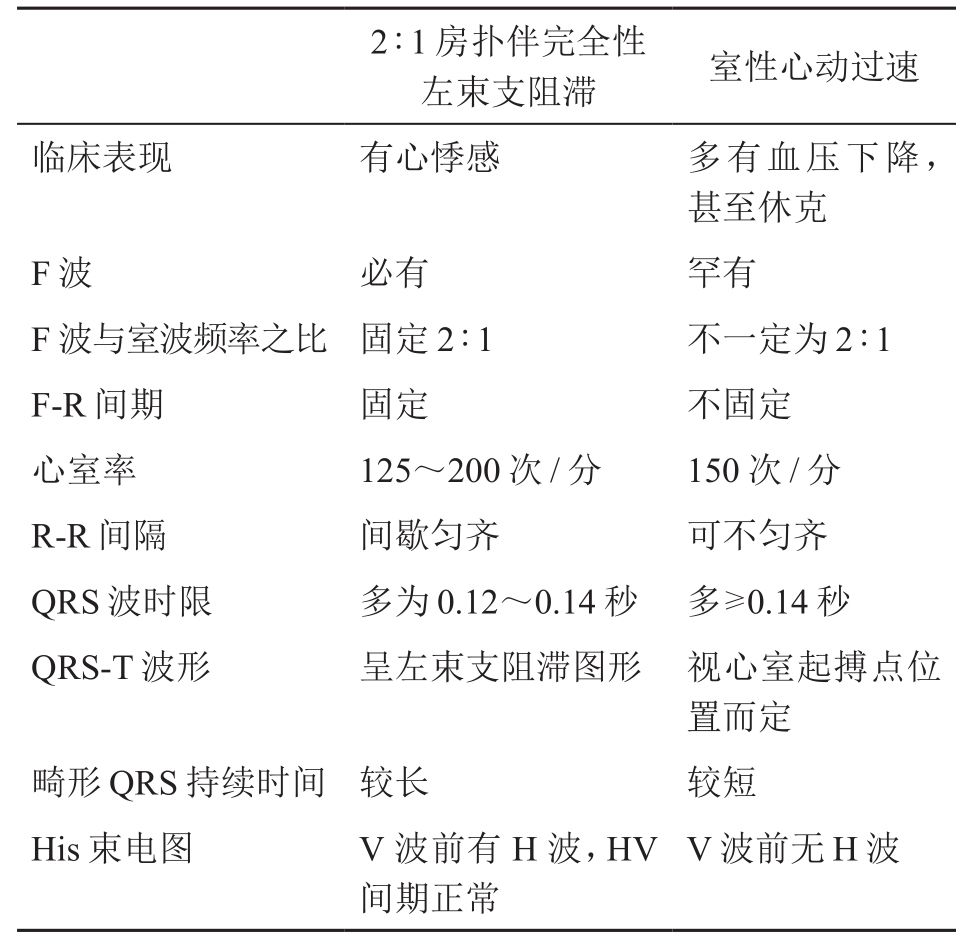
\includegraphics[width=3.25in,height=3.15625in]{./images/Image00424.jpg}
\end{table}

\subsection{治疗}

房扑治疗的目的是将其转复为窦性心律,预防复发或单纯减慢心率以缓解临床症状。

\subsubsection{非药物疗法}

\paragraph{直流电同步复律}

是治疗房扑最有效措施,成功率达90\%~100\%。房扑发作时有心绞痛、晕厥或其他血流动力学不稳定表现者,宜首选直流电击复律;对持续性房扑药物无效者,亦宜用电复律。推荐应用≤50J,有时可考虑首次应用100J,100J几乎总能一次成功,且极少造成危害。

\paragraph{心房快速起搏}

如电复律无效,或已应用大剂量洋地黄不适宜电复律者,可行心房快速起搏(将电极导管插至食管的心房水平,或经静脉穿刺插入电极导管至右心房处,以超过心房扑动频率起搏心房),能使大多数典型房扑转复为窦性心律或心室率较慢的房颤。但对于房扑伴1∶1房室传导或旁路快速前向传导,由于快速心房起搏可诱发快速心室率甚至室颤而应禁忌行心房快速起搏。

\paragraph{射频消融}

射频消融可根治房扑,因房扑的药物疗效有限,对于症状明显或引起血流动力学不稳定的房扑,应选用射频消融治疗。

\subsubsection{药物治疗}

对血流动力学状态稳定的患者,应首先以降低心室率为治疗目标。可用洋地黄、β受体阻滞剂、维拉帕米、胺碘酮等药物以增加房室传导阻滞的程度,控制心室率。

\paragraph{洋地黄制剂}

是房扑伴心功能不全者的首选药物。可用毛花苷丙0.4~0.6mg稀释后缓慢静注,必要时于2小时后再给0.2~0.4mg,使心室率控制在100次/分以下后改为口服地高辛维持。房扑大多先转为房颤,于继续用或停用洋地黄过程中,可能恢复窦性心律;少数从房扑转为窦性心律。

\paragraph{钙拮抗剂}

首选维拉帕米,5~10mg稀释后缓慢静注,偶可直接复律,或经房颤转为窦律,口服疗效差。亦可应用地尔硫{}
。

\paragraph{β受体阻滞剂}

艾司洛尔、普萘洛尔、阿替洛尔、美托洛尔等β阻滞剂延长房室交界区不应期和减慢房室传导,减慢心室率。

\paragraph{ⅠA(如奎尼丁)或ⅠC(如普罗帕酮)类抗心律失常药物}

能有效转复房扑并预防复发,但应事先以洋地黄、钙拮抗剂或β受体阻滞剂减慢心室率,否则,由于奎尼丁减慢心房率和对抗迷走神经作用,反而使心室率加快。如房扑患者合并冠心病、心力衰竭等时,应用ⅠA和ⅠC类抗心律失常药物易导致严重室性心律失常。此时,应选用胺碘酮:0.2g每日3次口服1周;减为0.2g每日2次口服1周;再减为0.2g每日1次口服;维持量0.2g/d,每周5~7天,对预防房扑复发有效。索他洛尔(80~320mg/d)亦可用于房扑预防,但不宜用于心肌缺血或左室功能不全的患者。如房扑持续发作,Ⅰ类与Ⅲ类药物均不应持续应用,治疗目标旨在减慢心室率,保持血流动力学稳定。

\paragraph{对于房扑伴 1∶1房室传导,多为旁道快速前向传导}

可选用延缓旁道传导的奎尼丁、普罗帕酮(心律平)、普鲁卡因胺、胺碘酮等,而禁用延缓房室结传导而旁道传导增加而加快室率的洋地黄和维拉帕米等。

\subsubsection{抗凝治疗}

原则与心房颤动相同。推荐应用华法林,使INR达2~3(参见本章第4节“心房颤动”部分)。

\subsubsection{病因治疗}

\hypertarget{text00290.htmlux5cux23CHP10-2-3-4}{}
参 考 文 献

1. 马爱群 ,胡大一.心血管病学.北京:人民卫生出版社,2005:119

2. 陆再英,钟南山.内科学.第7版.北京:人民卫生出版社,2008:193

\protect\hypertarget{text00291.html}{}{}

\section{心房颤动}

心房颤动(房颤,atrial
fibrillation,Af)是指心房丧失了正常的、规则的、协调的、有效的收缩功能而代之以350~600次/分的不规则颤动,是最常见的基本异位节律。WHO将其定义为:“心房律紊乱的无规则的电活动,心房波不明显,基线由一系列不规则的形态、间期和幅度变化的波形组成;未出现高度或完全性房室传导阻滞时,心室律不恒定且呈完全无规律状态。”绝大多数见于器质性心脏病的患者,其中以风湿性心瓣膜病、冠心病和高血压性心脏病最为常见。房颤在人群中的总发生率约0.4\%,65岁以上老人房颤发生率为3\%~5\%,60岁以后每10年发病率增加1倍,80岁后发病率可达8\%~10\%。合并房颤后心脏病死亡率增加2倍,如无适当抗凝,脑卒中增加5倍。

\subsection{病因与发病机制}

\subsubsection{病因}

\paragraph{心血管疾病}

多数房颤发生在心血管疾病基础上。常见的有:

\hypertarget{text00291.htmlux5cux23CHP10-2-4-1-1-1-1}{}
(1) 风湿性心瓣膜病:

是引起房颤最常见的病因之一。风湿性心瓣膜病导致房颤的原因与心房扩大、心房压力升高及心房肌病变有关。

\hypertarget{text00291.htmlux5cux23CHP10-2-4-1-1-1-2}{}
(2) 冠心病:

冠心病的所有类型均可发生Af。当出现心肌梗死、心肌硬化、合并充血性心力衰竭时,Af的发生率大为增加。AMI并发Af的发生率约11\%,一般认为高龄、心肌坏死范围大、心肌缺血严重、心功能障碍、PCWP及左心房压升高、心肌酶学明显升高、存在右束支阻滞合并室性心律失常时,更易出现Af。

\hypertarget{text00291.htmlux5cux23CHP10-2-4-1-1-1-3}{}
(3) 高血压性心脏病:

Af的发生与原发性高血压所致肥厚心肌的心电生理异常,肥厚心肌缺血及肥厚心肌纤维化有关。由于心肌肥厚及纤维化,心室顺应性减退,心房压升高及左房增大,加重心肌缺血,从而诱发房性电生理紊乱而导致Af。

\hypertarget{text00291.htmlux5cux23CHP10-2-4-1-1-1-4}{}
(4) 心肌病:

几乎所有不同类型的心肌病均可发生Af,发生率约为15\%~25\%。

\hypertarget{text00291.htmlux5cux23CHP10-2-4-1-1-1-5}{}
(5) 心肌炎:

心肌炎可出现各种类型心律失常,少数患者出现Af,心肌的炎症浸润、心肌缺血、心功能下降等均可作为诱发Af的原因。

\hypertarget{text00291.htmlux5cux23CHP10-2-4-1-1-1-6}{}
(6) 先天性心脏病:

各种先天性心脏病中,以房间隔缺损的Af发生率最高,约为20\%。随着年龄增长,Af发生率有逐步升高趋势,60岁以上者,高达52\%。

\hypertarget{text00291.htmlux5cux23CHP10-2-4-1-1-1-7}{}
(7) 缩窄性心包炎:

一般患者Af的发生率约为35\%,高龄患者可高达70\%。其他心包疾患,如心包积液也可伴发房颤。

\hypertarget{text00291.htmlux5cux23CHP10-2-4-1-1-1-8}{}
(8) 病态窦房结综合征:

Af的发生率高达38\%。

\hypertarget{text00291.htmlux5cux23CHP10-2-4-1-1-1-9}{}
(9) 心脏手术:

在冠脉搭桥术后Af发生率可高达25\%;二尖瓣狭窄患者在行瓣膜分离术后,Af的发生率达24\%~47\%;在瓣膜置换术后约32\%患者发生Af。通常发生Af的患者为高龄、术前曾有阵发性房颤发作或存在一定程度的二尖瓣关闭不全。

\hypertarget{text00291.htmlux5cux23CHP10-2-4-1-1-1-10}{}
(10) 其他心血管疾病:

包括感染性心内膜炎、二尖瓣脱垂、二尖瓣环钙化、心脏肿瘤等。

\paragraph{非心血管疾病}

包括:①代谢性疾病:如甲亢、甲减、低血糖等;②电解质紊乱:如低钾血症,低镁血症等;③呼吸系疾病:如肺心病,肺栓塞,阻塞性睡眠呼吸暂停综合征等;④风湿性疾病:如风湿热,系统性红斑狼疮,强直性脊椎炎等,由于其累及心肌及传导系统,可产生Af;⑤乙醇:是引起阵发性房颤的常见原因之一;⑥低温和拟交感类药物等。

\paragraph{其他}

包括:①家族性房颤:约占5\%。最早Af的基因定位于染色体10q22-q24,但陆续发现其他基因位点,表明家族性Af可能是多基因。②自主神经性房颤:自主神经系统通过提高迷走神经或交感神经张力可以触发易感患者发生Af。许多患者Af发作都是出现在迷走神经和交感神经张力增强的时候。③特发性房颤:也称孤立性房颤,是一种排除性诊断,即房颤无原因可查。一般认为此种房颤是良性的、功能性的、不合并器质性心脏病。

\subsubsection{发病机制}

1896年
Engelmann首次提出房颤可能是心房内一个局灶的兴奋点持续发出快速不规则冲动引起的,即房颤局灶起源学说;1921年Levis和Garrey提出房颤的发生机制主要是折返,即折返机制学说。这两种理论为以后半个多世纪房颤发生机制的研究奠定了基础,在此基础上相继提出过主导转子学说、自律性增高学说等机制。目前得到公认的有两种:①多发微波折返(multiple
wavelet
re-entry)学说:1962年Moe等提出:多发微波以紊乱方式经过心房,互相碰撞、再启动和再形成,并有足够的心房组织块来维持折返;②快速发放冲动灶(rapid
firing focus)学说:1997
年Haissaguerre等提出:左、右心房,肺静脉、腔静脉、冠状静脉窦等开口部位,或其内一定距离处(存在心房肌袖)有快速发放冲动灶,驱使周围心房组织产生房颤,由多发微波折返机制维持,快速发放冲动停止后房颤仍得以维持。

至今仍无一种学说能够解释所有Af的发生机制,可能Af本来就是多种机制并存和综合作用的结果。

\subsubsection{维持机制}

心房重构使Af发生后得以维持:①电生理重构:心房肌不应期缩短,其离散度增加,动作电位时程缩短,使Af持续或终止后再启动,发作间期延长直至持久性(房颤连缀现象,atrial
fibrillation begets atrial
fibrillation)。此外,Af还抑制窦房结功能,增加异位搏动发生和再启动房颤的能力。Af终止后电重构约在一周后消失;②组织结构重构:Af发作中的心房增大,心房肌萎缩、纤维化等,有利于Af的维持。心房肌局部肾素-血管紧张素-醛固酮系统激活,可促进间质纤维化;③离子通道重构:心房肌细胞离子通道发生功能性变化,成为维持Af的功能性基质,也可能是Af启动的机制。钠离子通道密度下降,钙先超负荷然后钙离子通道密度下降,使传导速度减慢,有效不应期缩短,动作电位时程缩短,Af易于维持。钾离子通道的种类多,其变化较为复杂,其中Ikur(超速激活钾通道)仅存在于心房肌,可能有较大影响。

\subsubsection{自主神经介导的房颤}

心肌电活动的稳定性有赖于迷走神经与交感神经活动的平衡,而二者任何一方活动过度增强都可产生致心律失常作用。实验证明:肾上腺素可降低心房肌动作电位除极幅度,而乙酰胆碱可使心房肌不应期缩短,且分布更不均匀,动作电位幅度增高。因此,迷走神经介导的阵发性房颤主要是心房肌不应期的缩短和较大折返环形成,表现为房扑,进而恶化为房颤;而交感神经介导的房颤主要由于心房肌兴奋性增高,触发激动及小折返环形成,因而可表现房速与房颤的混合存在。正常的心脏是迷走神经活动占优势,因此对正常的心房组织主要是受迷走神经的影响,迷走神经活动减弱常常是器质性心脏病早期特点之一;而对于病变的心房组织,更多见的是交感神经活动的异常。自主神经系统在阵发性房颤发生中的作用主要是由于心房肌对其介质的敏感所致,而不是自主神经系统本身的疾病所引起。

房颤的血液流变学改变是由于室律不规则,心动周期的明显不同导致每搏输出量不同,心动周期短则心室压力、充盈量、心输出量均降低,产生的低血压和心率过快又使冠脉血流量减低,心房有效收缩丧失、房室瓣关闭不全形成一定程度回流、血栓栓塞等均使全身血流动力学恶化。近年注意到,长期持续的房颤导致的心房肌细胞变性等,可使心房加压泵(booster
pump)功能和贮槽(reservoir)功能严重受损,彩色多普勒血流显像(CDEI)技术显示左心耳至左心房血流速度正常时为50cm/s,房颤时血流速度≤15cm/s,左心耳的收缩驱动功能几乎丧失。

房颤可产生严重的临床后果:①不良的血流动力学使心输出量降低15\%~40\%;②促使血栓栓塞和休克,加重或诱发心绞痛或心衰;③损伤左室收缩功能,提高总体及心脏病的死亡率。

\subsection{诊断}

\subsubsection{临床表现特点}

\paragraph{症状}

与原有心脏功能和心室率快慢有关。轻者可仅有心悸、气促、乏力、胸闷;重者可致急性肺水肿、心绞痛、心源性休克甚至昏厥,尤其WPW合并房颤或原有严重心脏病的患者。阵发性房颤者自觉症状常较明显。房颤伴心房内附壁血栓者,可引起栓塞症状。

\paragraph{体征}

主要是心律完全不规则,心音强弱不等;心室率多快速,120~180次/分。当心室率<
90次/分或>
150次/分时,节律不规则可不明显。排血量少的心搏不能引起桡动脉搏动,因而产生脉搏短绌(脉搏次数少于心搏次数),心率愈快则脉搏短绌愈明显。

一旦房颤患者的心室律变得规则,应考虑以下的可能性:①恢复窦性心律;②转变为房性心动过速;③转变为房扑(固定的房室传导比例);④发生房室交界区性心动过速或室性心动过速。如心室律变为慢而规则(30~60次/分),提示可能出现完全性AVB。ECG检查有助于确诊。房颤患者并发房室交界区性心动过速或室性心动过速或完全性AVB,最常见原因为洋地黄中毒。

\subsubsection{心电图特点}

其特点有:①P波消失,代之以形态、间距及振幅均绝对不规则的心房颤动波(f波),频率350~600次/分,通常在Ⅱ、Ⅲ、AVF或V\textsubscript{3}
R、V\textsubscript{1~2}
导联上较明显。②R-R间期绝对不规则,心室率较快;但若并发完全性房室传导阻滞或非阵发性交界处性心动过速时,R-R可规则,此时诊断依靠f波的存在。③QRS波群呈室上性,时限正常。但若合并预激综合征、室内差异性传导和束支传导阻滞时,QRS波增宽、畸形,此时心室率又很快时,极易误诊为室速,食管导联心电图对鉴别诊断很有帮助。④在长R-R间期后出现的短R-R间期,其QRS波群呈室内差异传导(常为右束支传导阻滞型)称为Ashman现象;差异传导连续发生时称为蝉联现象。⑤房颤未接受药物治疗、房室传导正常者,心室率通常在100~160次/分之间。

房颤合并其他心律失常时的心电图特点有:①合并单源性室性期前收缩:室性期前收缩波形相同,QRS波时限>
0.12秒;联律间期<
0.8秒;类代偿间期较一般f波下传的R-R间期长。②合并多形性室性期前收缩:室性期前收缩的形态和联律间期不等。③合并多源性室性期前收缩:室性期前收缩呈两种以上形态,联律间期>
0.8秒。④合并单形性室速:QRS时限>
0.12秒;波形相同;R-R周期基本匀齐;室率约160次/分;波形与单个或成对室早形态相同。⑤合并多源性室速:QRS-T呈两种以上形态,波形与多源性室性期前收缩相同;多见于洋地黄或奎尼丁过量、电解质紊乱等。⑥合并房室脱节:房颤与加速的交界性或室性逸搏、阵发性交界性心动过速、室速等并存,形成干扰性房室脱节。若出现交界性或室性逸搏心律,常提示合并二度或三度房室传导阻滞而致阻滞性房室脱节。

\subsubsection{房颤的分型}

根据美国心脏病学会/美国心脏协会/欧洲心脏病协会(ACC/AHA/ESC)联合制订的房颤指南,将房颤分为急性房颤与慢性房颤:

初次发作的房颤(recent Af)且在24~48小时以内,称为急性房颤。

慢性房颤可分为三类:①阵发性房颤(paroxysmal Af):持续时间<
7天(通常在48小时内),能自行终止,反复发作;②持续性房颤(persistent
Af):持续时间>
7天,或以前转复过,非自限性,反复发作;③永久性房颤(permanent
Af):不能终止,终止后又复发,或患者无转复愿望,持久发作。

除上述分类外,临床上尚可作以下分型:

\hypertarget{text00291.htmlux5cux23CHP10-2-4-2-3-1}{}
(一) 按病因分型

\paragraph{继发性房颤}

继发于各种疾病或其他因素时。

\paragraph{原发性房颤}

又称特发性房颤,指无明确病因引起者。

\hypertarget{text00291.htmlux5cux23CHP10-2-4-2-3-2}{}
(二) 按f波型分型

\paragraph{粗波型房颤(f波> 0.1mV)}

多见于甲亢、风湿性心瓣膜病及新近发生的房颤。

\paragraph{细波型房颤(f波< 0.1mV)}

多见于冠心病及持久性房颤者。

\hypertarget{text00291.htmlux5cux23CHP10-2-4-2-3-3}{}
(三) 按心室率的快慢分型

\paragraph{较慢型房颤}

在不伴有明显房室阻滞的房颤病例中,凡心室率在60~100次/分之间者,称为较慢型房颤。心房颤动时,一系列快速的f波在房室交界处产生的干扰、隐匿性传导以及房室结的“闸门作用”,是产生心室率较慢的电生理基础。此型房颤见于:①慢性心房颤动,可能合并有一度房室阻滞,对此洋地黄类药物应慎用。②心脏传导系统有退行性病变,或由于迷走神经张力增高,均可使更多的f波受阻于房室交界处不能下传心室,出现较慢的心室率。多见于老年患者。

\paragraph{快速型房颤}

凡心室率在100~180次/分之间的房颤,称为快速型房颤。短阵发作的或新近发生的房颤多属于此型,也是各型房颤中最常见的一种类型。此型房颤易发生室内差异性传导。

\paragraph{极速型房颤}

凡心室率在180次/分以上的房颤,称为极速型房颤。此型房颤常在下列情况下出现:①原为快速型房颤,由于运动使心室率加快转为极速型房颤;活动终止后心室率又恢复到原来频率。此种情况多见于各种原因引起的、未经治疗的、新近发生的房颤。②房颤合并预激综合征。③房颤合并加速的房室结传导现象。

\subsubsection{诊断注意事项}

根据心电图上P波消失,代之以f波的心电图特征,即可作出房颤的诊断。但应注意与以下几种情况鉴别:

1.房颤伴蝉联现象与房颤伴室速的鉴别(表\ref{tab102-5})。

2.房颤伴室内差异性传导时须与房颤伴发的室性期前收缩鉴别(表\ref{tab102-6})。

\begin{table}[htbp]
\centering
\caption{房颤伴蝉联现象与房颤伴室速的鉴别}
\label{tab102-5}
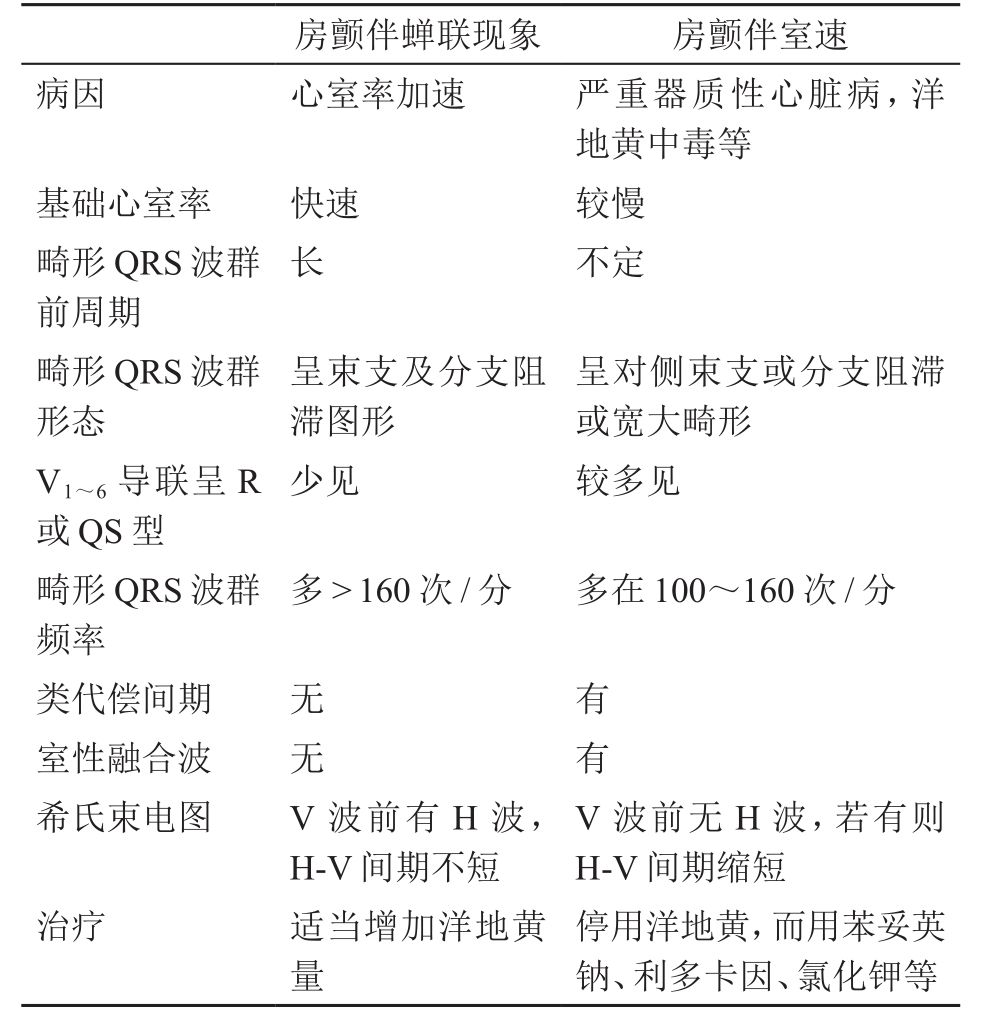
\includegraphics[width=3.30208in,height=3.36458in]{./images/Image00426.jpg}
\end{table}

\begin{table}[htbp]
\centering
\caption{心房颤动合并室内差传与室性期前收缩的鉴别}
\label{tab102-6}
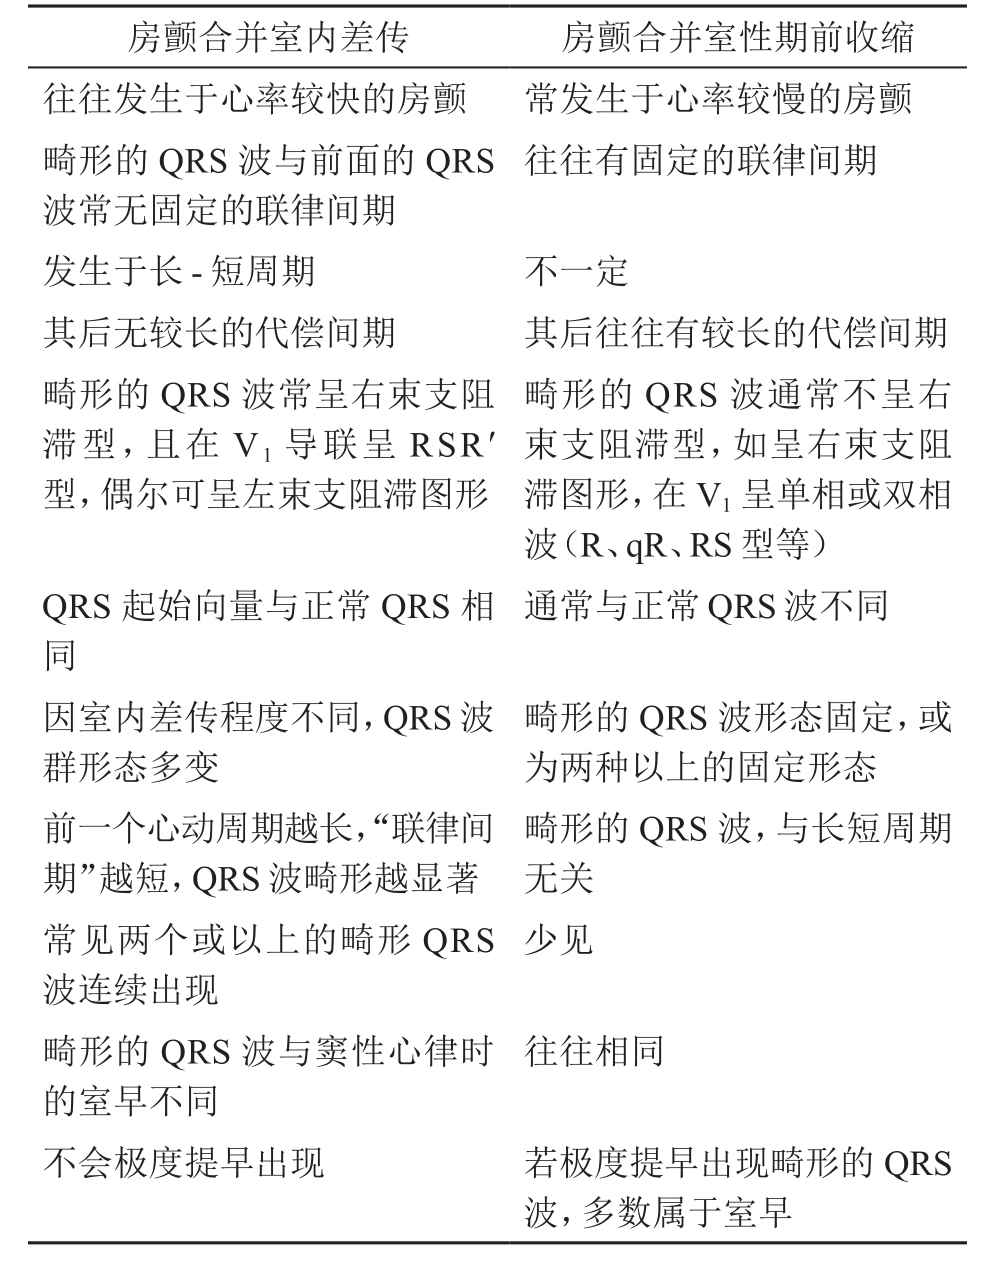
\includegraphics[width=3.27083in,height=4.20833in]{./images/Image00427.jpg}
\end{table}

3.迷走型与交感型自主神经性房颤的鉴别(表\ref{tab102-7})。

\begin{table}[htbp]
\centering
\caption{迷走型与交感型自主神经性房颤的鉴别}
\label{tab102-7}
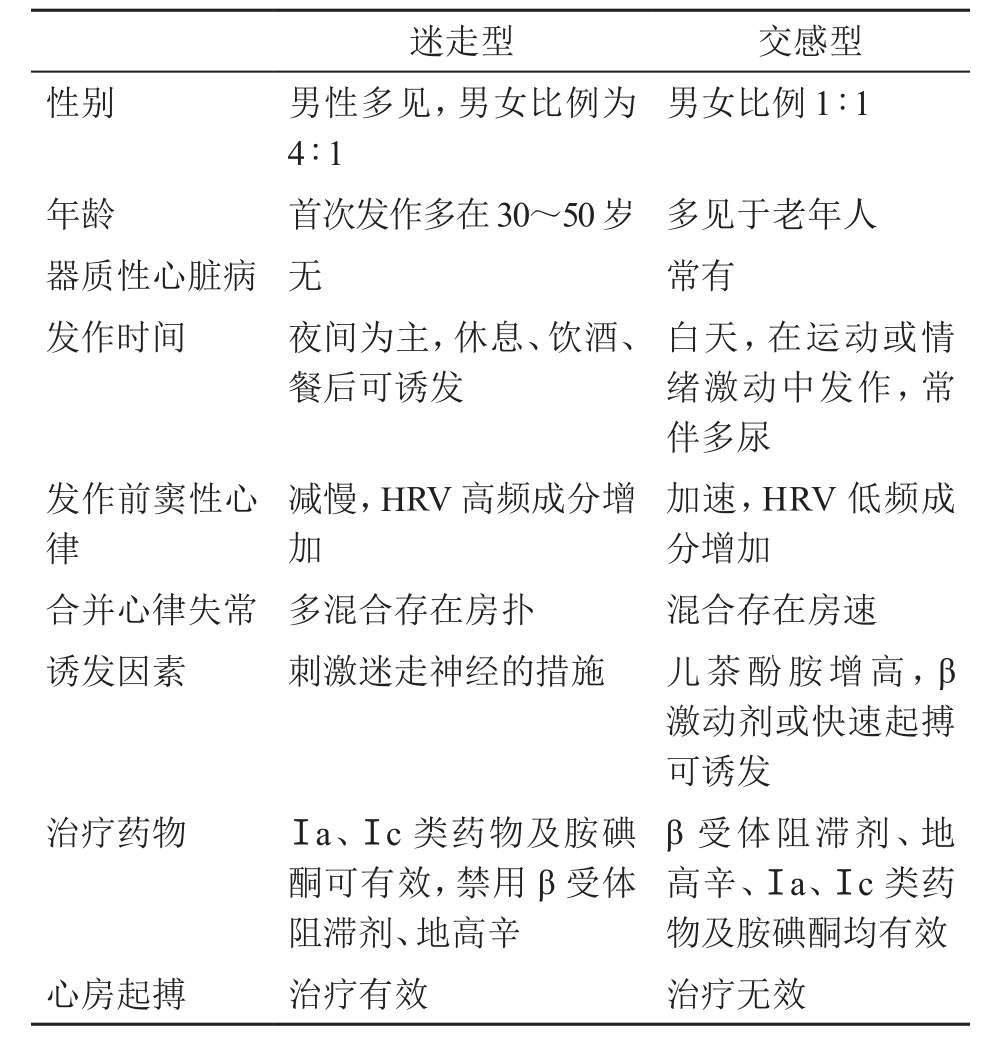
\includegraphics[width=3.26042in,height=3.45833in]{./images/Image00428.jpg}
\end{table}

HRV为心率变异性

\subsection{治疗}

房颤的治疗目的是消除或减轻症状,提高运动耐量和生活质量,预防血栓栓塞和心力衰竭并发症,降低房颤的致残率和死亡率。治疗目标是减少血栓栓塞和控制症状,后者主要是控制房颤时的心室率和(或)恢复及维持窦性心律。

\subsubsection{各型心房颤动的治疗原则与措施选择}

\hypertarget{text00291.htmlux5cux23CHP10-2-4-3-1-1}{}
(一) 急性心房颤动

\paragraph{治疗措施选择}

具体的治疗方案选择取决于患者的一般情况,主要是患者的血流动力学状况。对于血流动力学不稳定的患者,恢复并维持窦性心律是最为关键的一步。对以下状况:心室率大于150次/分、持续胸痛、收缩压低于90mmHg、心衰、意识不清者,应使用直流电复律,药物治疗仅作为二线方案。在电复律前应注意予以抗凝治疗,使用低分子肝素或普通肝素均可,如使用普通肝素可静脉注射给予3000~5000单位,调整剂量使APTT达到对照的1.5~2倍。电复律后是否继续使用抗凝药物取决于患者血栓形成的风险大小。

对于一般情况可,血流动力学稳定的患者,治疗主要应注意缓解症状及预防并发症,具体说来主要是心室率控制、节律控制及抗凝药物的使用。

对于超过48小时未自行复律或持续时间未知的心房颤动,在需要直流电或药物复律前应给予华法林3周(目标INR
2.0~3.0),复律后继续服华法林4周,避免左心房耳内血栓脱落或形成新的血栓。

\paragraph{控制心室率的药物治疗}

对于症状显著者,应迅速给予治疗。短期迅速控制心室率,使安静时心室率保持在60~80次/分,轻微运动后不超过100次/分。部分Af患者心室率控制后,可能自行转复为窦性心律。常用的药物有:

\hypertarget{text00291.htmlux5cux23CHP10-2-4-3-1-1-2-1}{}
(1) 毛花苷丙:

是伴有心力衰竭、肺水肿的快速Af首选药物,但必须首先排除WPW并发Af,并问清患者近期内有无用过洋地黄类药物。用法:0.2~0.4mg静注,必要时2~6小时可重复使用。若近期内曾口服洋地黄制剂者,可在密切观察下给毛花苷丙0.2mg。

\hypertarget{text00291.htmlux5cux23CHP10-2-4-3-1-1-2-2}{}
(2) 钙拮抗剂:

地尔硫{}
常采用“15法则”,即2分钟静注15mg,必要时15分钟后重复1次,继以15mg/h静滴维持,调整输液速度,使心室率达到满意的控制;或维拉帕米,用法是每10分钟静注5~10mg,必要时30~60分钟后重复1次。应注意这两种钙拮抗剂均有一定的负性肌力作用,可导致低血压,维拉帕米更明显,一般伴有明显心力衰竭者不用维拉帕米。

\hypertarget{text00291.htmlux5cux23CHP10-2-4-3-1-1-2-3}{}
(3) β受体阻滞剂:

普萘洛尔用法是1mg于5分钟内静注,必要时每5分钟可重复,最大剂量可达5mg,维持剂量为每4小时1~3mg;或美托洛尔5mg,5分钟内静注,必要时5分钟可重复,最大剂量10~15mg;或艾司洛尔0.25~0.5mg/kg静注(>
1分钟),续以50μg(/kg•min)静滴维持。

上述药物应在心电监护下静脉应用,心室率控制后应继续口服该药进行维持。地尔硫{}
或β受体阻滞剂与毛花苷丙联合治疗能更快并有效控制心室率,且毛花苷丙的正性肌力作用可减轻地尔硫{}
和β受体阻滞剂的负性肌力作用,使伴有心力衰竭患者更为安全。经上述处理后,房颤常在24~48小时内自行转复,仍未能恢复窦性心律者,可应用药物或电击复律。

\paragraph{特殊情况下房颤的治疗}

\hypertarget{text00291.htmlux5cux23CHP10-2-4-3-1-1-3-1}{}
(1) 预激综合征(WPW)伴房颤:

控制心室率避免使用β受体阻滞剂、钙拮抗剂、洋地黄和腺苷等药物,因这些药物阻断房室结的传导、房颤通过旁路下传使心室率反而增快。对心功能正常者,可选用胺碘酮、普罗帕酮、普鲁卡因胺或依布利特(ibutilide)等抗心律失常药物,使旁路传导减慢从而降低心室率,恢复窦律。胺碘酮用法:静注负荷量150mg(3~5mg/kg),10分钟注入,10~15分钟后可重复1次,继以1.0~1.5mg/min,静滴1小时,以后依病情逐渐减量,24小时总量一般不超过1.2g。应注意监测血压和心率,尤其是用于心功能明显障碍或心脏明显扩大者时。WPW伴Af心室率显著增快引起血压降低,甚至晕厥,或伴有心衰、肺水肿时应紧急处理,首选同步直流电复律,无条件时只有胺碘酮可以选择。

\hypertarget{text00291.htmlux5cux23CHP10-2-4-3-1-1-3-2}{}
(2) 急性心肌梗死伴房颤:

提示左心功能不全,可静注毛花苷丙或胺碘酮以减慢心室率改善心功能。如伴有严重血流动力学障碍或难治性心绞痛,应尽快同步电复律。

\hypertarget{text00291.htmlux5cux23CHP10-2-4-3-1-1-3-3}{}
(3) 甲亢伴房颤:

首选针对病因予以积极的抗甲亢药物治疗。由于甲状腺素对β受体阻滞剂的刺激作用,应选用非选择性的β受体阻滞剂如卡维地洛等。

\hypertarget{text00291.htmlux5cux23CHP10-2-4-3-1-1-3-4}{}
(4) 心脏病手术并发房颤:

术前给予口服β受体阻滞剂可以预防术后Af的发生。术后伴发Af以β受体阻滞剂为首选。

\hypertarget{text00291.htmlux5cux23CHP10-2-4-3-1-1-3-5}{}
(5) 妊娠伴发房颤:

可用地高辛、β受体阻滞剂或钙拮抗剂控制心室率。

\hypertarget{text00291.htmlux5cux23CHP10-2-4-3-1-1-3-6}{}
(6) 急性肺部疾患或慢性肺部疾病伴发房颤:

应纠正低氧血症和酸中毒,尽量选用钙拮抗剂控制心室率。Af导致血流动力学不稳定时同步直流电复律。

急性房颤诊疗流程见图\ref{fig102-8}。

\begin{figure}[!htbp]
 \centering
 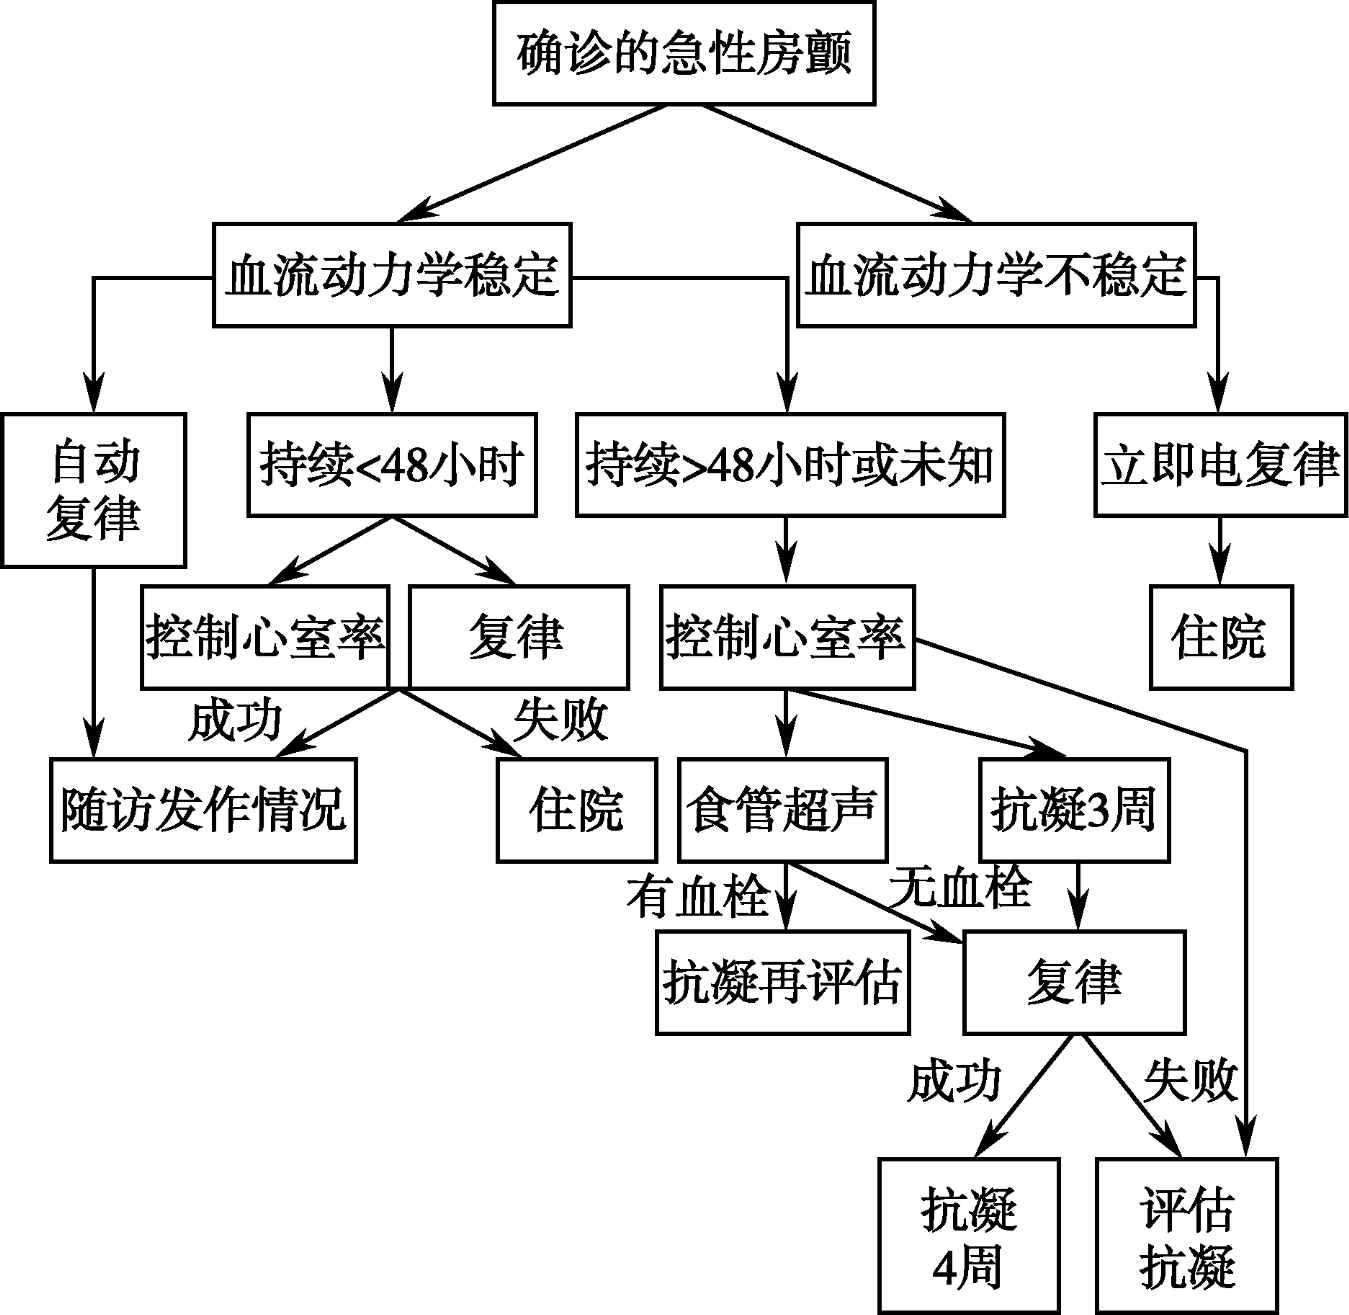
\includegraphics[width=3.11458in,height=3.04167in]{./images/Image00432.jpg}
 \captionsetup{justification=centering}
 \caption{急性房颤诊疗流程}
 \label{fig102-8}
  \end{figure} 

\hypertarget{text00291.htmlux5cux23CHP10-2-4-3-1-2}{}
(二) 慢性房颤

\paragraph{阵发性心房颤动}

发作期治疗的主要目标是控制心室率和转复窦性心律;非发作期(窦性心律时)的治疗目标是预防或减少心房颤动的发作。

阵发性心房颤动在无器质性心脏病(称为孤立性心房颤动)时:休息、镇静以及抗心律失常药物的应用,大多数患者均可转复为窦性心律,仅少数需用电复律。反复发作者应考虑射频消融或全胸腔镜外科手术以达到根治目的。

阵发性心房颤动患者在伴有心脏病时,也可采用上述原则,但如发生了血流动力学障碍或充血性心力衰竭时,需立即转复为窦性心律。尤其当二尖瓣或主动脉瓣狭窄伴有明显血流动力学异常时,必须立即给予复律以防止或逆转肺水肿的发生。选择同步直流电复律,首次电击给予100J,第二次和以后的电击给予200J或更高。

如果患者的血流动力学稳定,则可静脉使用毛花苷丙(西地兰)、地高辛、β受体阻滞药或钙通道阻滞药来控制心室率。既往主张首选洋地黄,它对休息状态下心室率的控制有效,但对运动时的心室率不能良好控制,起效作用慢。现主张选用静脉推注维拉帕米或地尔硫{}
,因为它们起效快,并能较好地控制运动时心室率。普鲁卡因胺、奎尼丁、丙吡胺对转复窦性心律有一定疗效,不良反应明显,已很少应用。伊布利特转复为窦性心律者较高,但必须在严密监测下应用,常需在用药后心电监护至少4小时,它可以急性延长QT间期,增加近期尖端扭转型室性心动过速的危险,索他洛尔也有明显的转复疗效。胺碘酮是目前公认的对复律及防止复发有明显疗效的药物。既往胺碘酮的使用受到限制主要在于它的副作用和过长的半衰期,后者限制了治疗的灵活性。现已证实小剂量的胺碘酮(200~300mg/d)可以明显地减少不良反应。

\paragraph{持续性心房颤动}

治疗目标:①转复窦性心律;②控制心室率加抗凝治疗。

持续性心房颤动发作时,尤其反复发作复律困难,如患者能较好耐受,无血流动力学障碍,多数学者不主张反复电复律。此时的治疗目标是控制复发时的心室率。ⅠA、ⅠC或Ⅲ类药物可预防心房颤动的复发,但是它们的疗效不稳定,而且还需考虑它们的致心律失常作用和不良反应。对于无器质性心脏病的患者可用ⅠC类药物,胺碘酮也有一定的疗效。根治手术可考虑射频消融术、全胸腔镜外科手术、外科小切口手术、外科迷宫手术。

\paragraph{慢性(永久性)心房颤动}

治疗目标主要是控制心室率,预防栓塞并发症。慢性心房颤动如果经药物或电复律治疗可使血流动力学改善,可在应用适量的抗心律失常药物(如胺碘酮、奎尼丁)后,尝试进行电复律。如在电复律治疗后仍转为慢性心房颤动者,要长期维持窦性心律的可能性则很小,对这类患者的治疗应侧重于控制心室率。根治手术有导管射频消融术、全胸腔镜外科手术、外科小切口手术、外科迷宫手术等。

\subsubsection{慢性心房颤动的长期心室率控制}

慢性心房颤动长期心室率控制,旨在延缓由于慢性房颤所致的心脏一系列改变,同时减轻患者心悸、气短和乏力等症状,以提高生活质量。心室率控制目标是静息时60~80次/分,日常活动时90~100次/分或中度活动后90~115次/分。常用的药物有β受体阻滞剂(如美托洛尔25~50mg口服,每天2次;普萘洛尔80~240mg/d,分3~
4次口服),地尔硫{}
(120~360mg/d,分次口服),维拉帕米(120~360mg/d,分次口服)和地高辛(0.125~0.375mg/d)等。普萘洛尔、美托洛尔、维拉帕米和地尔硫{}
均能有效控制Af患者静息和运动时的心室率。拉贝洛尔对控制静息时心室率无效,但对控制运动时心室率有效;地高辛对控制静息时心室率有效,因此,只能作为控制Af心室率的二线药物。对伴有高血压、缺血性心脏病患者首选β受体阻滞剂;无器质性心脏病,或不伴心力衰竭者,可选用地尔硫{}
或维拉帕米;伴有心力衰竭者,除选用地高辛治疗外,还可联用β受体阻滞剂治疗;对肥厚性心脏病患者,宜选用β受体阻滞剂或地尔硫{}
、维拉帕米治疗。口服胺碘酮长期治疗时副作用较多,不宜作为控制Af心室率的一线药物。

\subsubsection{心房颤动的复律治疗}

\hypertarget{text00291.htmlux5cux23CHP10-2-4-3-3-1}{}
(一) 复律适应证

复律适应证主要有 :①心房颤动持续1年以内,心脏扩大不显著(心胸比例<
0.5)且心力衰竭已纠正者;②超声心动图检测心房内无血栓,左心房内径<
45mm者;③基础病因去除后心房颤动持续存在者,如甲状腺功能亢进已控制(药物或手术根治后)、二尖瓣手术后;④因心房颤动出现使心力衰竭加重而用洋地黄制剂疗效欠佳者,或心房颤动出现诱发或加重心绞痛者;⑤有动脉栓塞史者;⑥心房颤动伴肥厚型心肌病者。

\hypertarget{text00291.htmlux5cux23CHP10-2-4-3-3-2}{}
(二) 复律禁忌证

复律禁忌证主要有
:①心房颤动持续1年以上;②心脏明显扩大或有明显心力衰竭者;③心房颤动严重二尖瓣关闭不全且左心房巨大者;④病因未去除者;⑤心房颤动心室率缓慢者(非药物影响);⑥合并病态窦房结综合征的阵发性或持续性心房颤动(慢-快综合征);⑦洋地黄中毒者。

\hypertarget{text00291.htmlux5cux23CHP10-2-4-3-3-3}{}
(三) 复律方法

\paragraph{药物复律}

Af发作在7天以内的患者药物复律的效果最好。大多数这样的患者Af是第一次发作,不少患者发作后24~48小时内可自行复律。Af时间较长的患者(>
7天)很少能自行复律,持续性Af患者药物复律的成功率也大大减少。

\hypertarget{text00291.htmlux5cux23CHP10-2-4-3-3-3-1-1}{}
(1) 胺碘酮:

胺碘酮负荷量有较大个体差异,临床医生可凭经验对不同的患者采取不同的给药方法,通常在推荐剂量下能达到良好疗效。胺碘酮转复心房颤动的给药方法:

静脉给药:胺碘酮静脉推注负荷量150mg(3~5mg/kg),10分钟注入,10~15分钟后可重复,随后1~1.5mg/min,静脉滴注6小时,其后减量至0.5mg/min维持。

口服给药:口服胺碘酮负荷量0.2g,每天3次,共7天,再以0.2g,每天2次,共7天,最后0.2g,每天1次长期维持。

部分患者,静注有效后可改为口服,如果静脉用药累计总量达10g者,口服剂量可直接改维持量。如未达累计量者,可根据情况0.2g,每天3次或0.2g,每天2次开始,明显超重者适当加量。

\hypertarget{text00291.htmlux5cux23CHP10-2-4-3-3-3-1-2}{}
(2) 普罗帕酮:

常规首剂35~70mg,稀释于5\%葡萄糖液20ml中缓慢静脉推注,10分钟后如不复律可重复一次,静注总量以不超过350mg为宜。也可试用口服复律法:每次150~200mg,每天3次;复律后改维持量每次100mg,每天3次。不良反应包括室内传导障碍加重、QRS波增宽、负性肌力作用,诱发或使原有心力衰竭加重,造成低心排血量状态。心肌缺血、心功能不全和室内传导障碍者相对禁用或慎用。

\hypertarget{text00291.htmlux5cux23CHP10-2-4-3-3-3-1-3}{}
(3) 索他洛尔:

以1.5mg/kg剂量稀释于生理盐水20ml中,缓慢静脉推注10分钟。观察30分钟,若未转复者可重复该剂量一次。转复率为30\%,未能转复者心室率均有所下降。口服:每次40~80mg,每天2次,通常日总量在160mg以下。不良反应:半衰期长,随剂量增加,扭转型室性心动过速发生率上升,低钾、低镁加重索他洛尔毒性作用。用药期间应监测心电图变化,当QTc≥0.55秒时,应考虑减量或暂时停药。窦性心动过缓、心力衰竭者不宜选用。

\hypertarget{text00291.htmlux5cux23CHP10-2-4-3-3-3-1-4}{}
(4) 依布利特(ibutilide):

用于转复近期发生的心房颤动,成人体重≥60kg者用1mg溶于5\%葡萄糖液50ml内静脉缓慢推注。如需要,10分钟后可重复一次。成人<
60kg者,以0.01mg/kg剂量按上法应用。心房颤动终止则立即停用。肝肾功能不全者无须调整剂量,用药应监测QTc变化,用药后至少心电监护4小时以上,注意尖端扭转性室速可能。

\hypertarget{text00291.htmlux5cux23CHP10-2-4-3-3-3-1-5}{}
(5) 决奈达隆:

结构和特征与胺碘酮相似,与胺碘酮相比,决奈达隆不含碘,安全性增加,亲脂性降低,半衰期显著缩短至约24小时,用量400mg,每天2次。决奈达隆转复房颤的效果可能较胺碘酮差。

\hypertarget{text00291.htmlux5cux23CHP10-2-4-3-3-3-1-6}{}
(6) 氟卡尼:

200~300mg口服。可能的副作用有:低血压、快速传导的房扑等。

\paragraph{直流电复律}

直流电同步电复律是安全有效的方法,几乎适用于所有首次发作的Af患者,成功率达80\%~95\%,合用药物几乎达到100\%。能量选择100~200J,力争一次复律成功。电复律后仍需药物来维持窦性心律。通常采用胺碘酮,在电复律前口服胺碘酮200mg,每天3次,共7天,电转复后,仍口服200mg,每天2次,共7天,再改成200mg,每天1次维持。电复律前服胺碘酮或普罗帕酮,可提高电复律成功率。

需指出的是:复律有引起血栓栓塞的危险,且药物复律与电复律发生血栓栓塞或脑卒中的危险性相同,两种复律方法的抗凝治疗相同。

\subsubsection{维持窦性心律预防复发的治疗}

药物维持窦性心律治疗的指征是阵发性Af或复律后Af复发伴有明显的症状,并且能够耐受抗心律失常药物治疗的患者。

\paragraph{维持窦性心律药物治疗的选择}

使用任何抗心律失常药物前,应分析有无Af可逆的心血管和非心血管因素。常见的因素有冠心病、瓣膜性心脏病、高血压和心衰。与饮酒有关的Af应戒酒。首次发现的Af发作很少需要预防性药物治疗,在发作较少且能够良好耐受的阵发性Af患者中也不必使用抗心律失常药物。同样,在已用药物治疗的患者中,如果Af很少复发和能够耐受,也不必换药。对于只在运动时发生Af者,服用β阻滞剂可能有效。但在多数情况下,Af的复发不是某个单一因素所致,不用抗心律失常药物就难以维持窦性心律。药物的选择首先应考虑其安全性和耐受性,此外应了解患者以前Af发作的次数和类型。

对于孤立性Af患者,可先试用β受体阻滞剂,但氟卡尼、普罗帕酮和索他洛尔更有效,胺碘酮和多非利特可作为替代治疗。除非胺碘酮无效,一般禁用奎尼丁、普鲁卡因胺和丙吡胺。但对于迷走神经介导的Af,有抗胆碱能作用的长效丙吡胺是一个较好的选择,氟卡尼和胺碘酮可分别作为第二和第三选择,但不宜用普罗帕酮,因后者有内在β阻滞活性,可能加重迷走神经介导的Af。对于交感神经介导的Af,首选β受体阻滞剂治疗,索他洛尔和胺碘酮可作为替代治疗。

\paragraph{某些心脏病患者维持窦性心律药物治疗的选择}

①心力衰竭:胺碘酮和多非利特被推荐用于心力衰竭患者窦性心律的维持。②冠心病:稳定的冠心病患者应首先考虑索他洛尔和胺碘酮,合并心衰者宜选用胺碘酮。③高血压性心脏病:伴有左室肥厚的患者可能增加发生尖端扭转性室速(TdP)的危险,后者与心室早期后除极有关。因此,宜选用不延长QT间期的药物。如无冠心病或无明显心室肥厚(左室壁厚度≤1.4cm)可选用氟卡尼、普罗帕酮和索他洛尔。胺碘酮延长QT间期,但致室性心律失常作用的危险性很低,考虑到其心外的副作用,在此类患者常作为二线治疗,但有明显左室肥厚存在时,胺碘酮则成为一线药物。如果胺碘酮和索他洛尔无效或不能使用时,则宜选择导管消融治疗。④预激综合征:WPW合并Af的患者宜行旁路射频消融治疗。⑤无或轻度器质性心脏病患者:可选用氟卡尼、普罗帕酮和索他洛尔。

\subsubsection{抗凝治疗}

心房颤动最常见、最严重的并发症是附壁血栓脱落造成重要器官的栓塞表现,特别是脑栓塞,它是导致心房颤动患者死亡的主要原因,目前的对策主要是抗凝治疗。

过去有栓塞病史、瓣膜病、高血压、糖尿病、老年患者、左心房扩大、冠心病等使发生栓塞的危险性更大。存在以上任何一种情况,均应接受长期抗凝治疗。风湿性心脏瓣膜病合并心房颤动,尤其是经过置换人工瓣膜的患者,应用抗凝剂预防血栓栓塞已无争议。对于其他情况是否需抗凝,也可以根据2010年ESC房颤指南推荐的CHA2DS2-VASc评分确定是否需要抗凝和选用药物。详见表\ref{tab102-8}和表\ref{tab102-9}。

华法林抗凝的INR目标值为2.0~3.0,华法林初始剂量2.5~3mg/d,2~4日起效,5~7日达高峰。华法林治疗开始后,每天监测INR,直到连续2天INR在目标范围内,然后监测2~3次/周,共1~2周,稳定后减少至1次/月。不适宜应用华法林的患者以及无以上危险因素的患者,可改用阿司匹林(81~325mg/d)。房颤持续不超过48小时,复律前无需作抗凝治疗,否则应在复律前行3周华法林治疗,待心律转复后继续治疗3~4周。紧急复律治疗可选用静注肝素或皮下注射低分子肝素抗凝。

对于出血高风险的中国患者,有学者和研究认为华法林抗凝INR目标值为1.6~2.5。出血风险评价可以参考2010年ESC房颤指南推荐的HASBLED评分评估,主要包括高血压、异常的肝肾功能、卒中史、出血、不稳定的INR、高龄、药物(抗血小板药物、非甾体抗炎药物等)或酗酒等,有上述因素的患者容易发生出血并发症。多项临床试验结果认为华法林口服剂量为5~10mg/d,保持凝血酶原时间的国际标准化比值(INR)为2.0~3.0,并强调个体化。中国人多数适合剂量为2.5mg/d,部分需大量或显著较小剂量,华法林基因检测分型有助于指导用药剂量以尽快达标。近年,有临床研究证实新的抗栓药物达比加群酯110mg每日2次效果优于华法林,而且无须检查,而阿哌沙班5mg,每日2次优于阿司匹林的抗栓效果。

\begin{table}[htbp]
\centering
\caption{CHA2DS2-VASc评分}
\label{tab102-8}
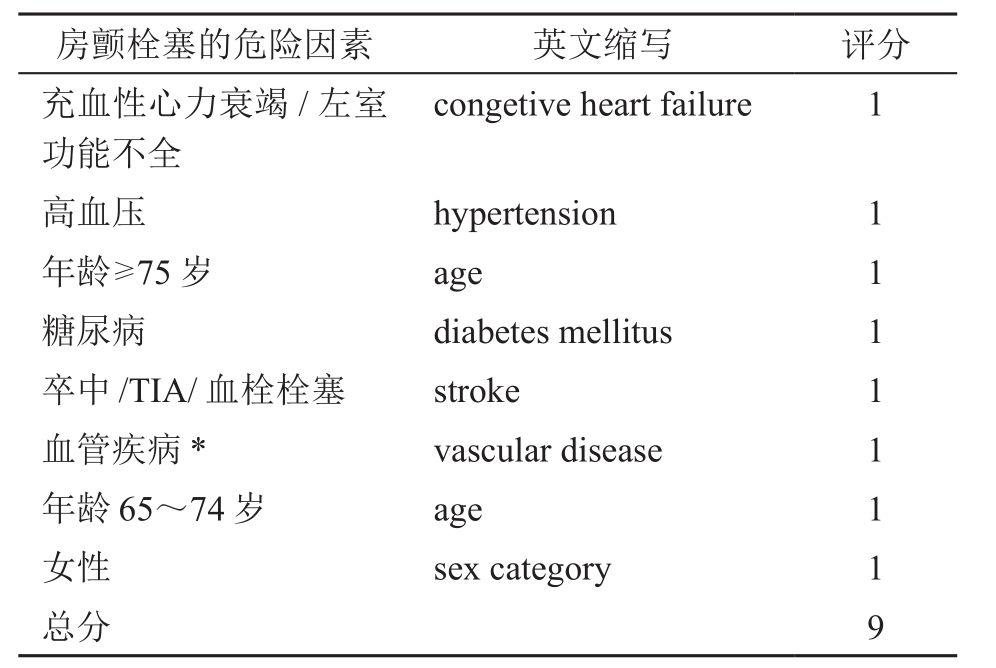
\includegraphics[width=3.3125in,height=2.21875in]{./images/Image00438.jpg}
\end{table}

*:血管疾病包括心梗、复杂的主动脉斑块、外周动脉疾病(含既往的血管再通、PAD截肢、造影证实的PAD等)

\begin{table}[htbp]
\centering
\caption{CHA2DS2-VASc评分与抗凝药物的选择}
\label{tab102-9}
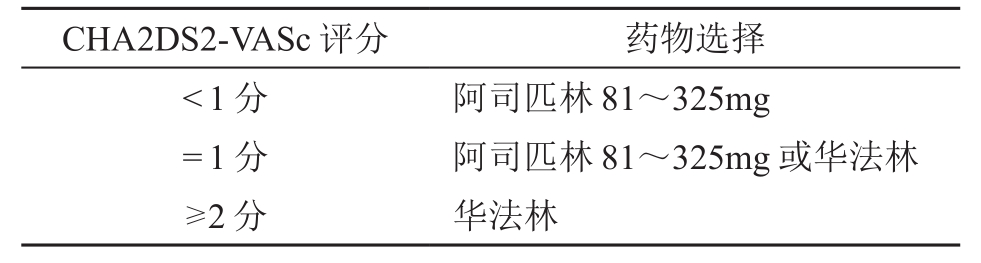
\includegraphics[width=3.26042in,height=0.86458in]{./images/Image00439.jpg}
\end{table}

\subsubsection{病因治疗}

如病因未控制,心房颤动难以消除,心室率也难以控制,故应积极治疗病因,包括甲状腺功能亢进、肺部感染、低氧血症、心脏瓣膜疾病等。

\hypertarget{text00291.htmlux5cux23CHP10-2-4-4}{}
参 考 文 献

1. Fuster V,Ryden LE,Cannom DS,et al. ACC/AHA/ESC 2006 Guidelines for
the Management of Patients with Atrial Fibrillation:a report of the
American College of Cardiology/American Heart Association Task Force on
Practice Guidelines and the European Society of Cardiology Committee for
Practice Guidelines(Writing Committee to Revise the 2001 Guidelines for
the Management of Patients With Atrial Fibrillation).
Circulation,2006,114(7):e257-e354.

2. Camm AJ,Kirchhof P,Lip GY,et al. Guidelines for the management of
atrial fibrillation:the Task Force for the Management of Atrial
Fibrillation of the European Society of Cardiology(ESC).
Europace,2010,12(10):1360-1420.

3. Fuster V,Rydén LE,Cannom DS,et al. 2011 ACCF/AHA/ HRS focused
updates incorporated into the ACC/AHA/ESC 2006 guidelines for the
management of patients with atrial fibrillation:a report of the
American College of Cardiology Foundation/American Heart Association
Task Force on practice guidelines.
Circulation,2011,123(10):e269-367.

\protect\hypertarget{text00292.html}{}{}

\section{室性心动过速}

室性心动过速(ventricular
tachycardia,VT),简称室速,为起源于希氏束分叉以下的束支、普肯耶纤维、心室肌的快速性心律失常。迄今为止,尚无一致公认的命名,目前国内大多采用Wellens等将其定义为:频率>
100次/分,连续3个或3个以上的室性期前收缩所组成的心律,如为程序心脏电刺激所诱发的室性心动过速,则必须是持续6个或6个以上的快速心室搏动(频率>
100次/分)。由于发作时心脏基础病变、心功能状态、频率及持续时间等的迥异,使其临床和预后有很大差别。室速虽非临床最常见的心律失常,但常导致严重血流动力学障碍,甚至因蜕变为心室颤动(ventricular
fibrillation,VF)而引起猝死,需及时正确的诊断和治疗。

\subsection{病因与发病机制}

VT常发生于各种器质性心脏病患者,最常见为冠心病,其次是心肌病、心力衰竭、二尖瓣脱垂、瓣膜性心脏病等,其他病因包括代谢障碍、电解质紊乱与长QT综合征等。VT偶可发生在无器质性心脏病者。

目前认为室速的发生机制主要为折返,少数为自律性增高或触发活动所致。

\paragraph{折返}

折返形成必须具备两条功能或解剖上相互分离的传导径路、部分传导途径的单向阻滞和另一部分传导缓慢这三个条件。心室内的折返可为大折返(macroreentry)-具有明确解剖学途径的折返(束支折返等),微折返(micro-reentry)-发生于小块心肌甚至于细胞水平的折返,后者为心室内折返最常见形式。

室速时的折返主要发生于正常工作心肌细胞和异常具有传导性的心肌组织间,折返性室速的频率冲动在折返环内传导速度和环长有关,而单向阻滞和慢传导均发生于异常组织中,可自发或因心率改变而产生。心肌的缺血、低血钾及代谢障碍等引起的心室肌细胞膜电位改变、动作电位时间、不应期、兴奋传导性的非均质性,使心肌电活动不稳而易诱发室速。

折返机制诱发的室速具有以下特点:①可为程序刺激所诱发;②可为程序刺激及超速起搏所终止;③心房刺激罕有诱发;④诱发室速的期前收缩联律间期与期前收缩距室速第一个QRS波间期呈反比关系;⑤诱发室速周期长度与程序刺激周期长度、期前刺激数目及期前联律间期无关;⑥存在“拖带”(entrainment)现象;⑦心室晚电位可阳性;⑧维拉帕米药效不确切。

\paragraph{自律性增高}

心肌缺血缺氧、心肌牵张均使心室异位起搏点4相舒张期除极化坡度提高而导致心室肌异常自律性或自律性增高;血儿茶酚胺浓度增高、细胞外液低钾及洋地黄作用可使希-普系统自律性增高。此类室速的电生理特点为:①运动、静滴异丙肾上腺素可诱发其发作;②程序刺激既不能诱发也不能终止其发作;③无“拖带”现象;④期前刺激周期与回响周期无关;⑤心室晚电位阴性;⑥维拉帕米治疗无效。

\paragraph{触发活动}

触发活动诱发的室速约占5\%,常由前一次去极化活动的早期后去极化或延迟后去极化所诱发。现较明确的与触发活动有关的室速包括多形性室速、洋地黄中毒所致室速及维拉帕米敏感性室速;再灌注诱发的室速仅发现于动物试验中。其电生理特点:①可为程序刺激诱发或终止;②与起搏频率有关;③常不表现为“拖带”现象;④诱发室速的期前收缩联律间期与回响周期呈正相关;⑤心室晚电位阳性;⑥维拉帕米常可终止或预防其发作。

\subsection{诊断}

\subsubsection{临床表现特点}

VT多由体位改变、情绪激动、突然用力或饱餐所诱发,亦可无明显诱因。VT的临床症状轻重视发作时心室率、持续时间、基础心脏病变和心功能状况不同而异。非持续性VT(发作时间短于30秒,能自行终止)的患者通常无症状。持续性VT(发作时间超过30秒,需药物或电复律始能终止)常伴有明显血流动力学障碍与心肌缺血,临床症状常见的有心悸、气促、心绞痛、低血压、少尿和晕厥,严重者表现为心衰和阿斯综合征发作。听诊心律可轻度不规则,第一、二心音分裂,收缩期血压可随心搏变化。如发生完全性室房分离,第一心音强度经常变化,颈静脉间歇出现巨大a波。当心室搏动逆传并持续夺获心房,心房与心室几乎同时发生收缩,颈静脉呈现规律而巨大的a波。

\subsubsection{心电图特征}

心电图是诊断VT的基石。VT的心电图特征有:①3个或以上的室性期前收缩连续出现;②心室率通常为100~250次/分,心律规则,亦可略不规则;③QRS波群形态畸形,时限增宽(0.12~0.18秒),约2/3的病例其QRS≥0.14秒;约2/3的室速其QRS呈右束支阻滞图形(V\textsubscript{1}
呈rsR'、qR或单相R波),1/3呈左束支阻滞图形(V\textsubscript{1}
以负向波为主,V\textsubscript{6}
以正向波为主)。少数病例其QRS形态均不符合左、右束支阻滞图形。ST-T波方向与QRS波群主波方向相反;④房室关系:半数室速发作时,呈现完全性房室分离(图\ref{fig102-9});另一半可见室房(VA)传导,其中大部为1∶1
VA传导,其余为2∶1或隐匿性VA传导;⑤额面电轴:VT发作时,约2/3的病例电轴左偏(−30°~−90°),其余电轴右偏或正常(二者各占一半);⑥心室夺获和室性融合波:VT发作时少数室上性冲动可下传心室,产生心室夺获,表现为在P波之后,提前发生一次正常的QRS波群。室性融合波的QRS波群形态介于窦性与异位心室搏动之间,其意义为部分夺获心室;⑦发作和终止:一般而言,室速发作突然。室速的第一个搏动通常是提前的,其形态与随后的QRS波相似,也可略有不同。如无治疗,持续性室速或自行终止,或蜕变为室颤。自行终止前,往往有几个搏动或几秒室速的频率和形态发生改变,蜕变为室颤前,常有室速频率的加快;⑧刺激颈动脉窦无反应。

\begin{figure}[!htbp]
 \centering
 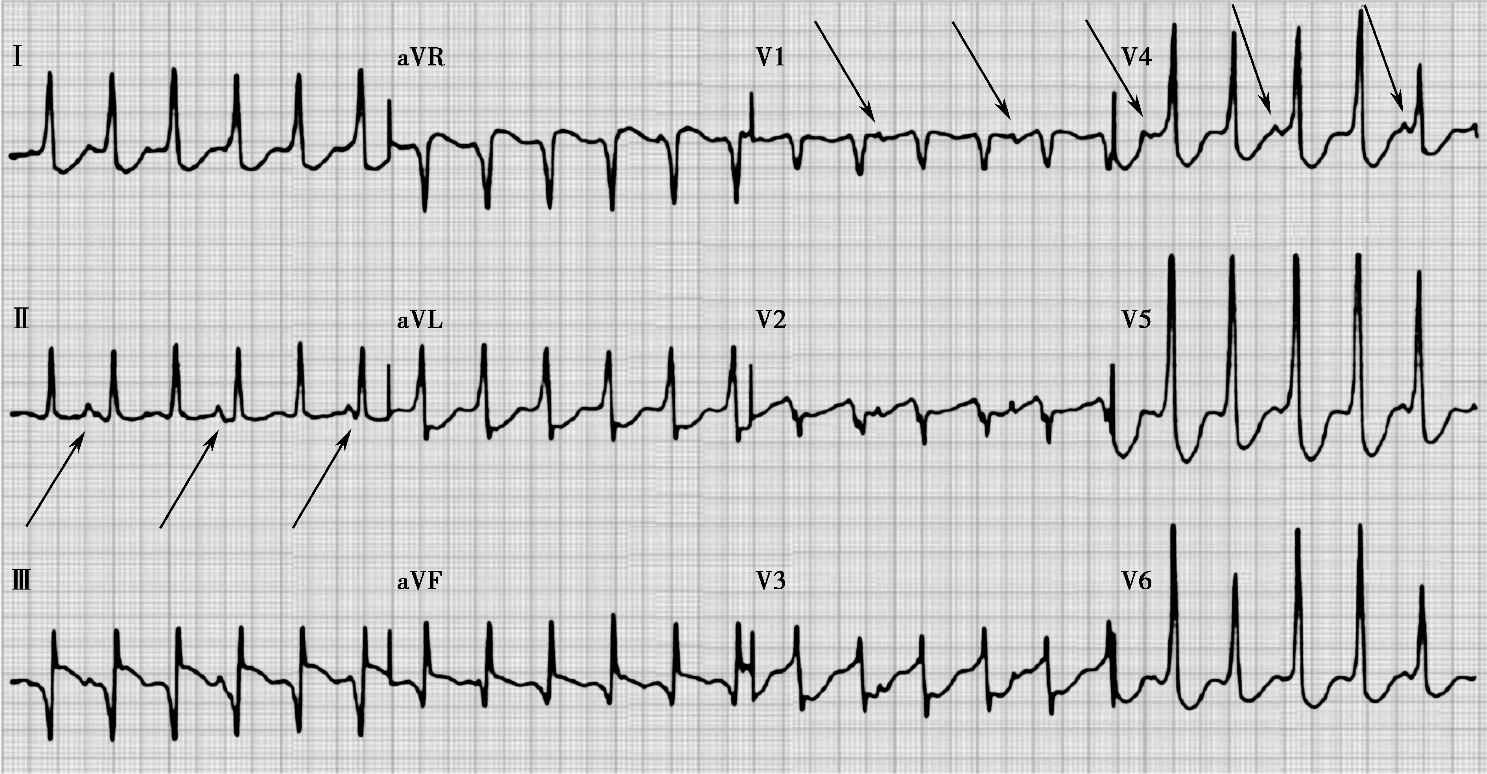
\includegraphics[width=6.29167in,height=3.27083in]{./images/Image00440.jpg}
 \captionsetup{justification=centering}
 \caption{室性心动过速}
 \label{fig102-9}
  \end{figure} 

图示房室分离和P波(箭头)与QRS波群无关

\subsubsection{室速的分类}

鉴于室速的病因、临床表现与心电图特点及治疗等方面存在有明显的差异,其临床分类方法颇多,如:

\hypertarget{text00292.htmlux5cux23CHP10-2-5-2-3-1}{}
(一) 按室速发病机制的不同

可分为
:①折返性室速:室速由心室内快速折返形成所致。折返是VT最常见的发生机制。②自律性室速:室速由室内异位起搏点自律性增高所致。见于加速性室性自主心律。③触发活动性室速:室速由心肌早期后除极和延迟后除极所致。主要见于由长QT间期综合征引起的尖端扭转型室速、洋地黄中毒引起的室速。

\hypertarget{text00292.htmlux5cux23CHP10-2-5-2-3-2}{}
(二) 根据室速发作持续时间的长短

可分为 :①持续性室速(sustained VT):室性搏动频率>
100次/分,时间持续30秒以上,不能自行终止;或虽持续时间<
30秒,但已出现血流动力学紊乱而需立即电复律者。还有少见的持续性室速,反复发作持续时间长,抗心律失常药物不能有效终止者,称为无休止性室速。②非持续性室速(non-sustained
VT):室性搏动频率> 100次/分,30秒内自行终止者。

\hypertarget{text00292.htmlux5cux23CHP10-2-5-2-3-3}{}
(三) 根据有无器质性心脏病

可分为
:①病理性室速:各种器质性心脏病导致的室速。根据引起VT的病因,可分为冠心病VT、心肌病VT、右心室发育不良性VT等。②特发性室速:发生在形态和结构正常的心脏的VT。根据发生部位,可分为左心室特发性室速和右心室特发性室速。

\hypertarget{text00292.htmlux5cux23CHP10-2-5-2-3-4}{}
(四) 根据室速发作时血流动力学的改变和预后分类

\paragraph{良性室速}

VT发作时未造成明显血流动力学障碍,发生心源性猝死的危险性很低。主要见于器质性心脏病患者。

\paragraph{潜在恶性室速}

非持续性但反复发作的VT,不常导致血流动力学障碍,但可能引起心源性猝死,患者大多有器质性心脏病的客观证据。

\paragraph{恶性室速}

反复发作持续性室速,造成明显血流动力学障碍,表现为黑矇、晕厥、心功能不全、心绞痛发作甚至猝死。常发生在心脏扩大、LVEF
< 30\%的患者。常见类型有多形性室速、尖端扭转型室速、束支折返性室速等。

\hypertarget{text00292.htmlux5cux23CHP10-2-5-2-3-5}{}
(五) 根据室速发作形式的不同

\paragraph{阵发性室速}

室速突然发生和终止,节律可整齐也可不整齐,心室率160~250次/分,QRS波形可为单形性、双向性和多形性。

\paragraph{非阵发性室速}

又称加速性室性自主心律、室性自搏性心动过速、缓慢型室速。其起始往往缓慢而非突然,是由于心室异位节律点的兴奋性高于窦房结所致。心室率通常为60~110次/分(偶有快达140次/分者),与窦性心律的频率接近,差异常在5~10次/分之内。常呈短阵发作,多以3~20个心动为一阵,与窦性心律交替出现,常见心室夺获及室性融合波。当窦性频率增快时,室性自主心律便被替代,反之,又出现室性自主心律。常见病因是急性下壁心肌梗死、急性心肌炎、高血钾、洋地黄中毒等,也可见于无器质性心脏病的患者。临床过程相对良好,常自动消失,罕见转为室颤,且不影响心功能。治疗以针对原发病为主,如必要,可首选阿托品以消除窦性心律不齐并加快窦性心律。利多卡因和普鲁卡因胺亦有效,但不常规应用,电复律无效。

\hypertarget{text00292.htmlux5cux23CHP10-2-5-2-3-6}{}
(六) 根据室速起源部位的不同

\paragraph{肌性室速}

室速起源于:①室间隔;②右室肌;③左室肌(前壁、侧壁、后壁、心尖部)。

\paragraph{分支性室速}

室速源于:①右束支;②左束支主干;③左前分支;④左后分支。

\hypertarget{text00292.htmlux5cux23CHP10-2-5-2-3-7}{}
(七) 根据室速发作时 QRS波群形态

\paragraph{单形性室速(monomorphic VT)}

是指室速发作时,QRS波群形态在ECG同一导联上单一而稳定,呈右束支传导阻滞或左束支传导阻滞图形。

\paragraph{多形性室速(polymorphic VT)}

是指室速发作时,QRS波群在ECG同一导联上出现三种或三种以上形态。由于VT频率快,可进展为VF,必须积极治疗。本组VT包括多种电生理机制,按VT发作前基础QT间期长度可分为以下两类:

\hypertarget{text00292.htmlux5cux23CHP10-2-5-2-3-7-2-1}{}
(1) 伴发于QT间期延长的多形性室速:

即尖端扭转型室速。参见本章第6节之“尖端扭转型室性心动过速”部分。

\hypertarget{text00292.htmlux5cux23CHP10-2-5-2-3-7-2-2}{}
(2) 伴发于QT间期正常的多形性室速:

又依室性期前收缩联律间距是否缩短分为以下两种:

\hypertarget{text00292.htmlux5cux23CHP10-2-5-2-3-7-2-2-1}{}
1) 联律间距“不短”的多形性VT:

多见于冠心病,VT发作可伴或不伴发于AMI。发病机制多数与折返活动有关。临床特征有:①VT呈多形性,基础心律时QT、T或U波正常;发作间歇期并非缓慢型心律;室性期前收缩的联律间距不长,亦“不短”(图\ref{fig102-10});②起搏对预防和治疗无效;③交感神经刺激(如应用异丙肾上腺素)可使病情恶化;④治疗药物与持续性单形性VT相同(包括Ⅰ、Ⅲ类药物);⑤必要时ICD治疗;⑥心肌血管再造术或抗心肌缺血药物对预防发作有帮助。

\hypertarget{text00292.htmlux5cux23CHP10-2-5-2-3-7-2-2-2}{}
2) 伴发于极短联律间距的多形性室速 :

发病机制与触发活动(早期后除极)有关。临床表现为心悸、眩晕、晕厥,反复发作可致死亡。主要特征有:①反复发作多形性VT,但并无器质性心脏病证据;②不论单一或诱发VT的室性期前收缩均显示有极短联律间距(通常在280~320ms之间),常发生在ST段终末或T波起始部;③基本心律中T或U波形态及QT间期均正常;④交感神经兴奋药物无效且可能加重发作;⑤Ⅰ、Ⅱ、Ⅲ类抗心律失常药通常无效;⑥静脉或口服维拉帕米对终止及预防发作十分有效。

\paragraph{双向性室速(bidirectional VT)}

是指室速发作时,在ECG的同一导联上QRS波群呈现两种形态并交替出现,表现为肢体导联QRS波群主波方向交替发生正负相反的改变,或胸前导联QRS波群呈现左、右束支传导阻滞图形并交替变化。双向性VT主要见于严重的器质性心脏病(如扩张型心肌病、冠心病等)或洋地黄中毒,该型VT患者的基本心律失常为心房颤动。

\hypertarget{text00292.htmlux5cux23CHP10-2-5-2-3-8}{}
(八) 按室速持续时间和形态的不同组合

\begin{figure}[!htbp]
 \centering
 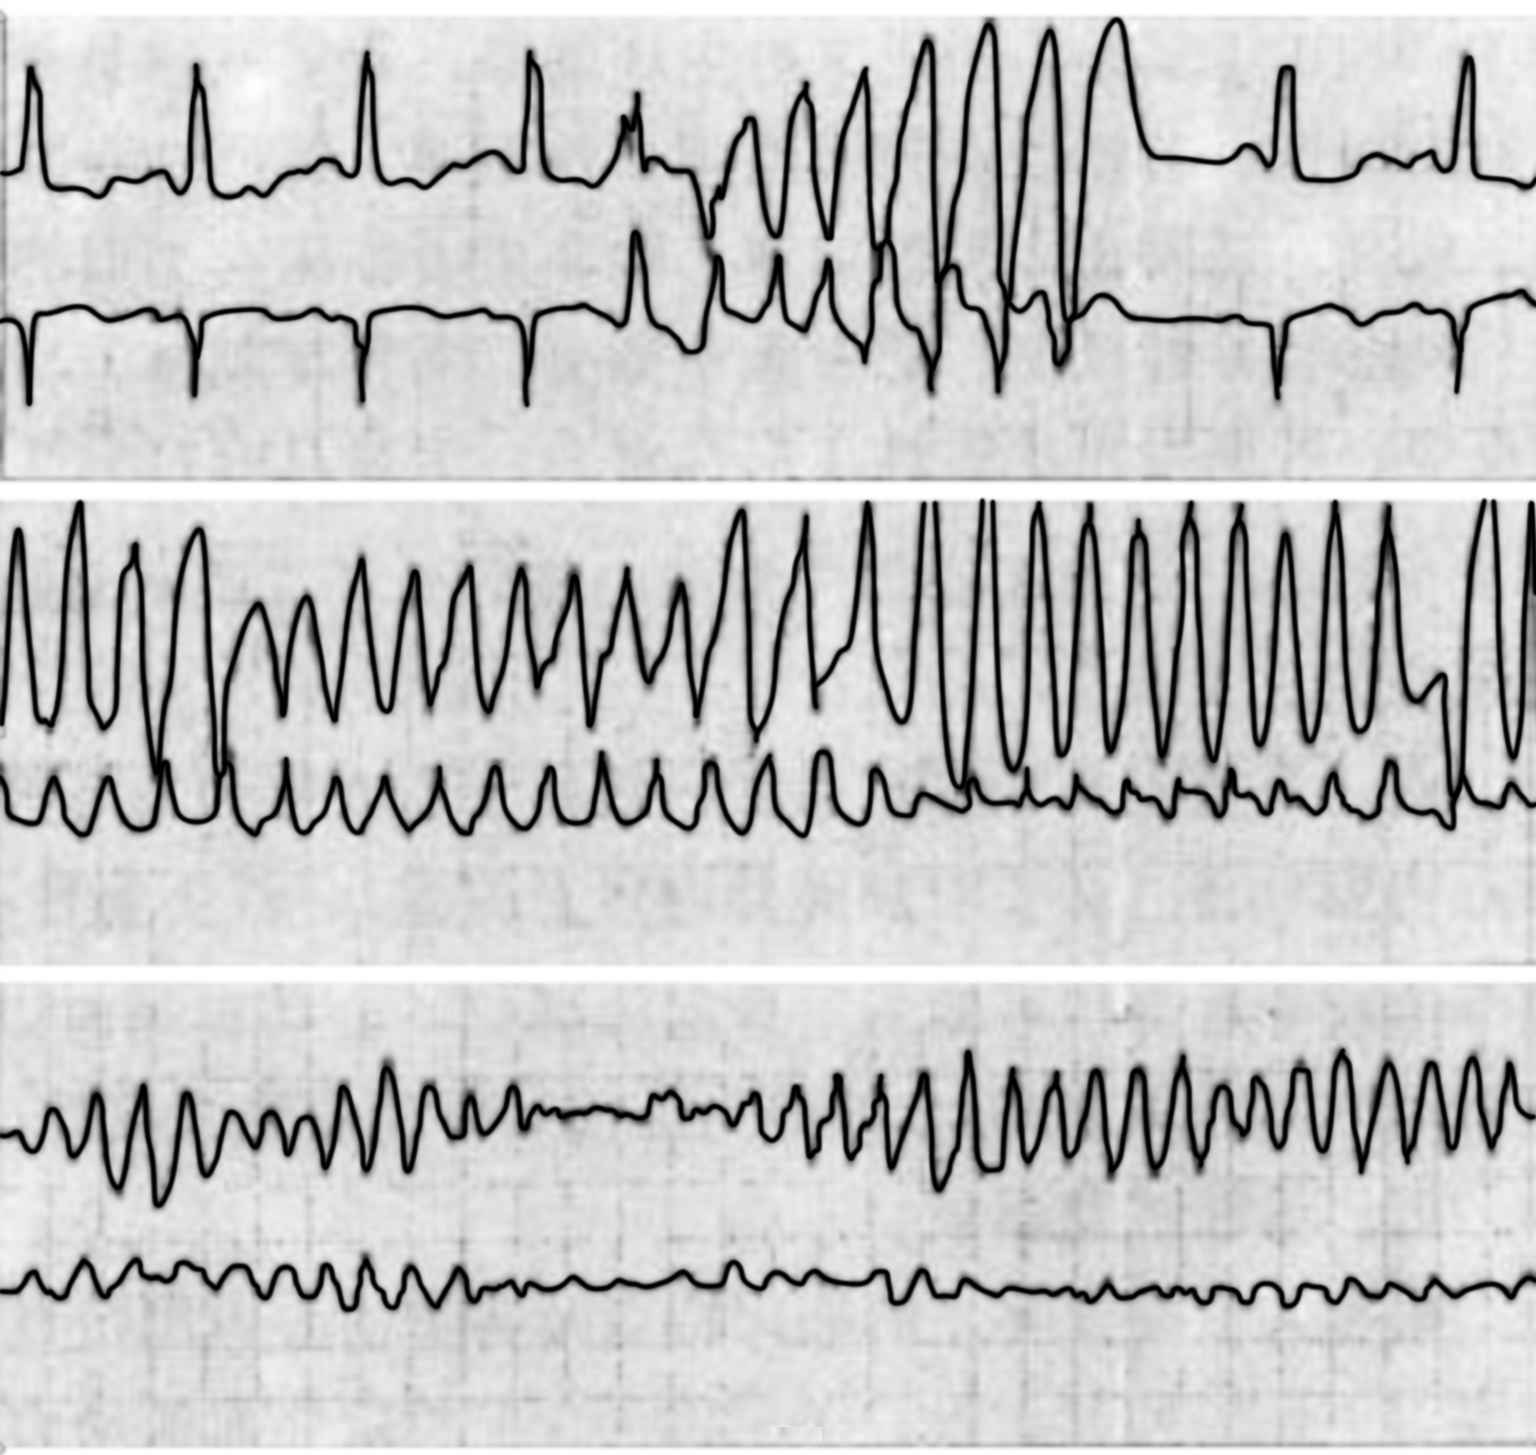
\includegraphics[width=5.72917in,height=5.42708in]{./images/Image00441.jpg}
 \captionsetup{justification=centering}
 \caption{冠心病心梗后反复发生多形性室速}
 \label{fig102-10}
  \end{figure} 

QT间期正常的自发性多形性室速(上),持续性发作(中)和导致室颤(下)

可分为:①单形性持续性室速;②单形性非持续性室速;③多形性持续性室速;④多形性非持续性室速。(图\ref{fig102-10})

若心室电生理程序刺激所诱发的1~5个非起搏性室性期前搏动则称为反复性心室反应(repetitive
ventricular response,RVR)。

\subsubsection{电生理学检查}

希氏束电图上H与V分离,与A-H间期常有固定关系;A-H频率慢于V波频率,即可诊为室速。

室速的电生理检查适用于反复发作的室速、存在心性猝死或因室速反复晕厥的患者,以及部分无症状而持续室速的患者,检查有助于室速的确诊并判断其性质,阐明发病机制,标测其起源部位和传导途径,寻找某些高危患者,筛选有效的抗心律失常药等。

\subsubsection{诊断注意事项}

根据VT突发突止的临床特点及典型的心电图特点,可作出室速的诊断。但临床上常因以下原因使其误诊:①误以为VT肯定伴血流动力学障碍;②仅靠单一导联的心电图图形诊断;③只靠房室分离诊断;④误以为室速为一不规律的心律失常;⑤忽略了QRS波形对室速的诊断价值。

VT虽然是宽QRS心动过速的最常见原因,但后者亦见于室上性心动过速(SVT)伴差异传导,或在原有束支传导基础上发生的SVT,或经旁道前向传导的房室折返型心动过速。支持VT诊断的ECG表现有:①心室融合波;②心室夺获;③室房分离;④全部心前区导联QRS波群主波方向呈同向性:即全部向上或向下;⑤发作时QRS波形态与原有束支传导阻滞的QRS波形态不一致。有利于SVT的表现包括:①心动过速反复发作而无器质性心脏病基础;②兴奋迷走神经的手法或药物使心动过速终止;③发作开始均可见提早的P波(室上性期前收缩);④发作时ECG示P与QRS间有固定关系,且心室活动依赖心房活动下传(如伴Ⅱ度Ⅰ型AVB);⑤发作时QRS形态在V\textsubscript{1}
为rsR′型(三相)而V\textsubscript{6}
为qRS或Rs型,QRS起始向量与窦律时一致。此外,心动过速在未用药物治疗前,QRS时限超过0.20秒,宽窄不一,心律明显不规则,心室率超过200
次/分,应怀疑为预激综合征合并房颤。

VT与预激综合征合并房颤,心室扑动的鉴别分别见表\ref{tab102-10}和表\ref{tab102-11}。

\subsection{治疗}

VT治疗一般遵循的原则是:有器质性心脏病或有明确诱因应首先给以针对性治疗;无器质性心脏病患者发生非持续性短暂VT,如无症状或血流动力学影响,处理原则与室早相同;持续性VT发作,无论有无器质性心脏病,应给予治疗。

\subsubsection{终止室速发作}

\paragraph{药物治疗}

血流动力学稳定的患者,一般先用药物治疗。常用的药物有:

\hypertarget{text00292.htmlux5cux23CHP10-2-5-3-1-1-1}{}
(1) 胺碘酮:

对伴有心功能不全的室速患者首选。用法:静注负荷量150mg(3~5mg/kg),10分钟注入,10~15分钟后可重复,随后1~1.5mg/min静滴6小时,以后根据病情逐渐减量至0.5mg/min。

\hypertarget{text00292.htmlux5cux23CHP10-2-5-3-1-1-2}{}
(2) 利多卡因:

50~100mg静脉注射,必要时每隔5~ 10分钟再给
50mg,直至心律转复或总量达300mg为止。有效后以1~2mg/min的速度静脉滴注,稳定后改用口服药物。禁忌证有严重房室传导阻滞与室内传导阻滞、利多卡因过敏等。

\begin{table}[htbp]
\centering
\caption{室速与预激综合征伴房颤的鉴别要点}
\label{tab102-10}
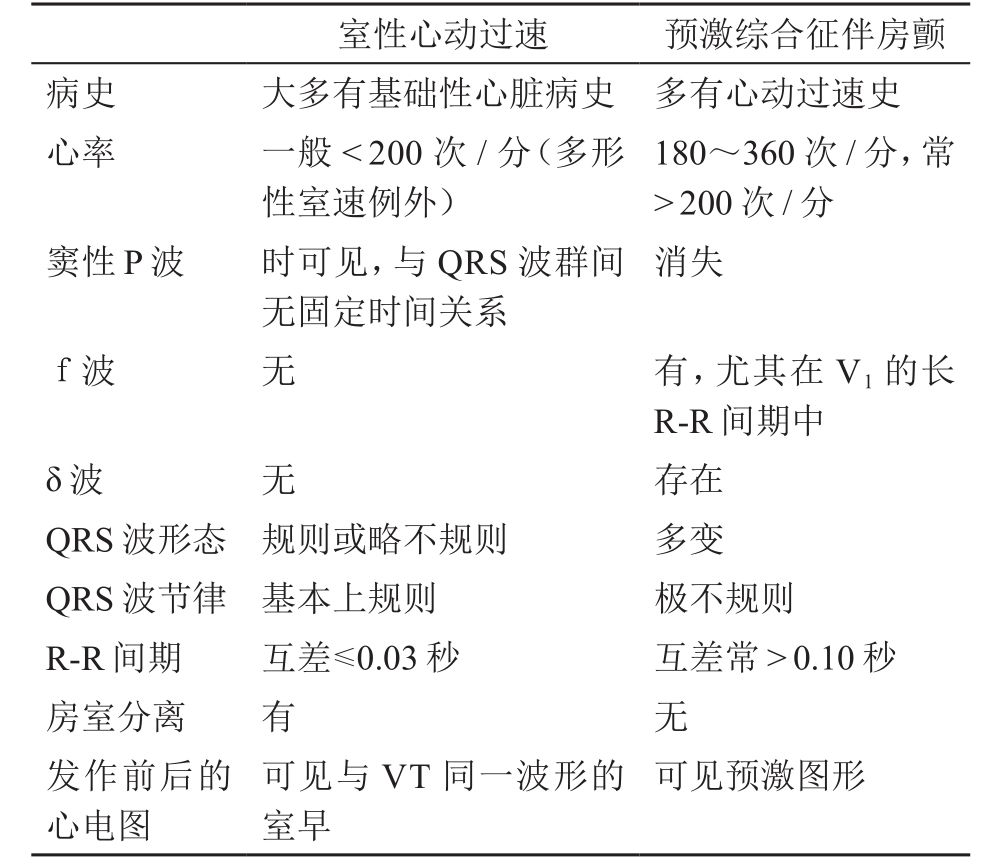
\includegraphics[width=3.28125in,height=2.86458in]{./images/Image00442.jpg}
\end{table}

\begin{table}[htbp]
\centering
\caption{心室扑动与室性心动过速的鉴别诊断}
\label{tab102-11}
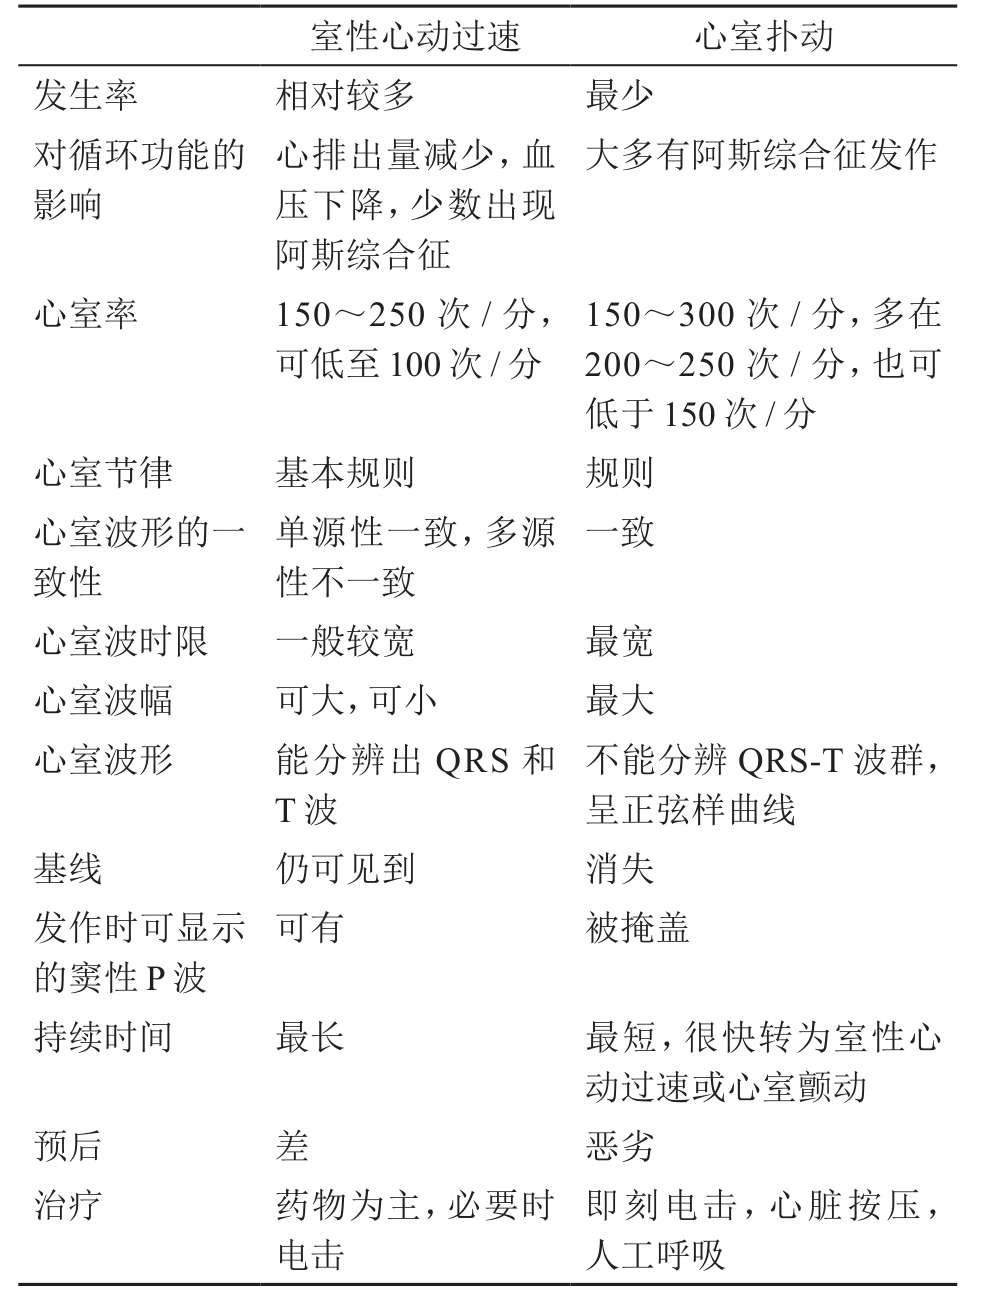
\includegraphics[width=3.30208in,height=4.35417in]{./images/Image00443.jpg}
\end{table}

\hypertarget{text00292.htmlux5cux23CHP10-2-5-3-1-1-3}{}
(3) 普鲁卡因胺:

100mg静注(3~5分钟内),每隔5~10分钟重复1次,直至心律失常被控制或总量达1~2g;或用普鲁卡因胺0.5~1.0g加入5\%葡萄糖液100ml中持续静滴(1小时内),无效者1小时后再给1次。在静脉应用过程中,应行血压和心电图监测,若血压明显下降或心电图QRS波群增宽时、或心律恢复后,应立即停止注射。主要副作用有低血压,窦房、房室传导阻滞,尖端扭转型室速等。禁忌证有严重低血压、心衰、Ⅱ度以上房室传导阻滞、肝肾功能不全等。

\hypertarget{text00292.htmlux5cux23CHP10-2-5-3-1-1-4}{}
(4) 苯妥英钠:

适用于洋地黄中毒患者。可用0.125~0.25g加入注射用水20~40ml中缓慢静注(5分钟以上),必要时重复静注0.125g,一日量不超过0.5g。禁忌证有低血压、高度房室传导阻滞(洋地黄中毒例外)、严重心动过缓等。

\hypertarget{text00292.htmlux5cux23CHP10-2-5-3-1-1-5}{}
(5) 普萘洛尔:

适用于心梗伴交感神经张力增高、甲亢、二尖瓣脱垂、梗阻性心肌病、肾上腺素能依赖性尖端扭转性室速的患者。用法:0.15mg/kg稀释后缓慢静注(<
1mg/min)。主要副作用有心动过缓、低血压等;禁忌证有心衰、低血压、高度房室传导阻滞、心动过缓、哮喘等。

\hypertarget{text00292.htmlux5cux23CHP10-2-5-3-1-1-6}{}
(6) 维拉帕米:

适用于梗阻性心肌病、“维拉帕米敏感性室速”的患者。用法:5~10mg/次稀释后缓慢静注(>
5分钟)。主要副作用有低血压、过缓性心律失常、诱发心衰、便秘等。禁忌证有心衰、低血压、心源性休克、房室传导阻滞等。

\hypertarget{text00292.htmlux5cux23CHP10-2-5-3-1-1-7}{}
(7) 普罗帕酮:

用法:1~1.5mg/(kg•次)(常用70mg)加入25\%葡萄糖液20~40ml中静注,10~20分钟后无效重复1次,一般静注总量不超过210mg。由于普罗帕酮有负性肌力作用及抑制传导系统作用,且个体间存在较大差异,对有心功能不全者应禁用,对有器质性心脏病、低血压、休克、心动过缓者等慎用或禁用。

\hypertarget{text00292.htmlux5cux23CHP10-2-5-3-1-1-8}{}
(8) 其他:

心力衰竭所致的VT,能排除洋地黄中毒者,可试用洋地黄治疗;VT继发于严重过缓性心律失常(如病窦综合征、完全性房室传导阻滞)者,静脉滴注异丙肾上腺素或心室起搏的疗效较心肌抑制药物治疗更好;锑剂中毒引起者,还可用大剂量阿托品治疗。

\paragraph{电学治疗}

紧急情况下,可用同步直流电复律、食管调搏、超速起搏抑制终止其发作。心脏直流电复律指征:①有血流动力学明显障碍者如低血压,心衰伴心源性休克,首选直流电复律;②用药物治疗未能迅速终止者;③VT持续时间长,已超过2小时者。同步直流电复律可迅速、可靠而安全地终止持续性VT发作,是终止伴严重血流动力学障碍或药物治疗无效的持续性VT的主要手段,即时成功率达98\%左右。但电复律不能预防发作,不适用于能自动终止但反复发作的非持续性VT。初次复律的电能量可用100~200J,以期1次电击复律成功。转复成功后尚需静脉滴注抗心律失常药物,以预防复发。洋地黄引起的VT宜先试用苯妥英钠或利多卡因静注,无效时再用低能量直流电复律。

\subsubsection{预防复发}

\paragraph{病因与诱因治疗}

应努力寻找和治疗诱发及使VT持续的可逆性病变,例如缺血、低血压及低血钾等。治疗充血性心力衰竭有助于减少VT发作。窦性心动过缓或AVB时,心室率过于缓慢时有利于VT的发生,可给予阿托品治疗或应用人工心脏起搏。

\paragraph{药物预防}

目前除了β受体阻滞剂、胺碘酮外,尚未能证实其他抗心律失常药物能降低心脏性猝死的发生率。维拉帕米(240~360mg/d)可用于“维拉帕米敏感性室速”的患者,此类患者通常无器质性心脏病基础,QRS波群呈右束支传导阻滞伴有电轴左偏。

\paragraph{射频消融术}

对于无器质性心脏病的特发性单源性VT导管射频消融根除发作疗效甚佳。

\paragraph{置入式心脏复律除颤器(implantable defibrillator,ICD)}

对心脏骤停后复苏存活的猝死高危患者及药物治疗无效的、有严重症状的VT反复发作患者,可显著降低猝死率和心血管总死亡率,但其价格昂贵,尚不能为大多数患者所接受。

\paragraph{外科手术治疗}

已设计多种外科手术方法以治疗室壁瘤或右室发育不良所致VT。手术的适应证包括致命性室速、曾有室颤史的冠心病患者、内科治疗难以控制的室速患者,心功能Ⅲ~Ⅳ级、室壁瘤、急诊手术者死亡率较高。手术方式包括心内膜环行心室肌切断术、心内膜切除术、冷冻外科手术等。

正确选择VT的各种治疗措施有赖于:①区别对待VT发作时症状严重与无症状的患者;②区别对待预后良好与预后差或猝死高危的患者;③熟悉各种治疗措施的疗效、风险及价格。必须结合不同类型VT给个体患者带来的风险,对比不同治疗措施的疗效、风险和价格,然后作出恰当的选择。心肌梗死后或心肌病伴症状严重的持续性VT反复发作,猝死危险性高而抗心律失常药物难以控制的宜及早考虑消融或埋藏式自动复律除颤起搏器治疗。特发性VT发作时症状严重的,大多先试抗心律失常药物治疗;而症状轻或无症状的,则无需长期药物治疗。

\hypertarget{text00292.htmlux5cux23CHP10-2-5-4}{}
参 考 文 献

1. Pellegrini CN,Scheinman MM. Clinical management of ventricular
tachycardia. Curr Probl Cardiol,2010,35(9):453-504

2. Roberts-Thomson KC,Lau DH,Sanders P. The diagnosis and management
of ventricular arrhythmias. Nat Rev Cardiol,2011,8(6):311-321

3. Hood RE,Shorofsky SR. Management of arrhythmias in the emergency
department. Cardiol Clin,2006,24(1):125-133

4. 曹林生 ,廖玉华.心脏病学.第3版.北京:人民卫生出版社,2010:418

5. 陆再英,钟南山.内科学.第7版.北京:人民卫生出版社,2008:204

\protect\hypertarget{text00293.html}{}{}

\section{几种特殊类型的室性心动过速}

\hypertarget{text00293.htmlux5cux23CHP10-2-6-1}{}
尖端扭转型室性心动过速

尖端扭转型室性心动过速(torsades de
pointes,TdP),简称尖端扭转型室速或扭转型室速,是一种特殊类型的快速性室性心律失常,通常发生在原发或继发性QT间期延长的基础上,其心电图特征、临床表现、发病机制、病因及治疗均与一般的室性心动过速或心室颤动不同。早年由于对这类室速的概念模糊不清,常被误为是心室颤动,故称之为“短暂性心室颤动”、“心室扑动颤动”等。直至1966年才由法国电生理学家Dessertenne对其作了系统描述,并命名为扭转型室速。但是,近年来随着心电监护及记录方法的提高,发现具扭转形态的室速并非均一同质的临床实体。有些室速,其QRS波呈典型扭转形态但基本心律中QT间期正常,其发病机制、治疗等也与QT间期延长者有很大差异,为了区别这两种扭转形态的室速,目前主张仅把伴QT间期延长者称为扭转型室速,而QT间期正常者称为多形性室速。

\subsection{病因与发病机制}

\subsubsection{病因}

伴QT间期延长的扭转型室速常谓之为长QT综合征(long QT
syndrome,LQTS),根据病因、起病方式及治疗的不同,Jackman(1985年)等将其分为间歇依赖性和肾上腺素能依赖性以及中间型(表\ref{tab102-12})。

\paragraph{间歇依赖性(获得性)LQTS}

病因包括:①药物引起:抗心律失常药物(奎尼丁、丙吡胺、普鲁卡因胺、氟卡尼、胺碘酮、索他洛尔、苄普地尔等),精神治疗药物如三环或四环类抗抑郁药、吩噻嗪类等,血管扩张剂心可定、利多氟嗪(lidoflazine),某些抗寄生虫药如灭虫宁、氯喹、酒石酸锑钾等,以及红霉素、有机磷杀虫药等;②电解质紊乱如低钾、低镁或低钙;③营养不良、饥饿或长期液体蛋白饮食;④严重的窦性心动过缓或病窦综合征,完全性或高度房室传导阻滞等。其临床特征为TdP几乎总发生在心搏暂停或心率突然减慢之后。

\paragraph{肾上腺素能依赖性(先天性)LQTS}

主要根据有无先天性耳聋及遗传性分为:①Jervell和Lang-Nielsen(JNL)综合征:有先天性神经性耳聋,常染色体隐性遗传。到目前为止,JLN综合征已发现有2种亚型,即JNL\textsubscript{1}
和JNL\textsubscript{2} ,其致病基因分别为KCNQ\textsubscript{1}
和KCNE\textsubscript{1} ,分别使心肌细胞离子流I\textsubscript{ks}
和I\textsubscript{kr}
减弱,使复极时间延长;②Romano-Ward综合征(RWS):无耳聋,常染色体显性遗传。到目前为止,已发现12个致病基因,1200余个突变位点。这12个致病基因分别为:LQT1(KCNQ1)、LQT2(hERG)、LQT3(SCN5A)、LQT4(Ankyrin-B)、LQT5(KCNE1)、LQT6(KCNE2)、LQT7(KCNj2)、LQT8(Cav1.2)、LQT9(Cav3)、LQT10
(SCN4B)、LQT11(AKAP)、LQT12(SNTA1)。临床上,以前3种最为常见,约占先天性LQTS的90\%~95\%,其中KCNQ1(LQT1)和hERG(LQT2)均通过负显性(dominant
negative)机制或功能丧失机制发挥作用,而SCN\textsubscript{5}
A(LQT\textsubscript{3} )突变使通道功能亢进(gain of
function)机制起作用,主要是钠通道失活延迟。③散发型:无耳聋,无家族史。此型共同特点与高水平的儿茶酚胺有关,多在剧烈运动、疼痛、惊恐或其他应激状态下发作,临床表现为反复晕厥,也可以阿-斯综合征开始,乃至心脏性猝死。此型还包括某些二尖瓣脱垂、脑血管意外等所发生的TdP。

\paragraph{中间型 LQTS}

有些患者TdP发作既可由儿茶酚胺类诱发,也与长间歇有关。部分患者的TdP发作时U波明显,但其前无长间歇,与运动及情绪无关。

\begin{table}[htbp]
\centering
\caption{长 QT间期综合征(LQTS)的分类}
\label{tab102-12}
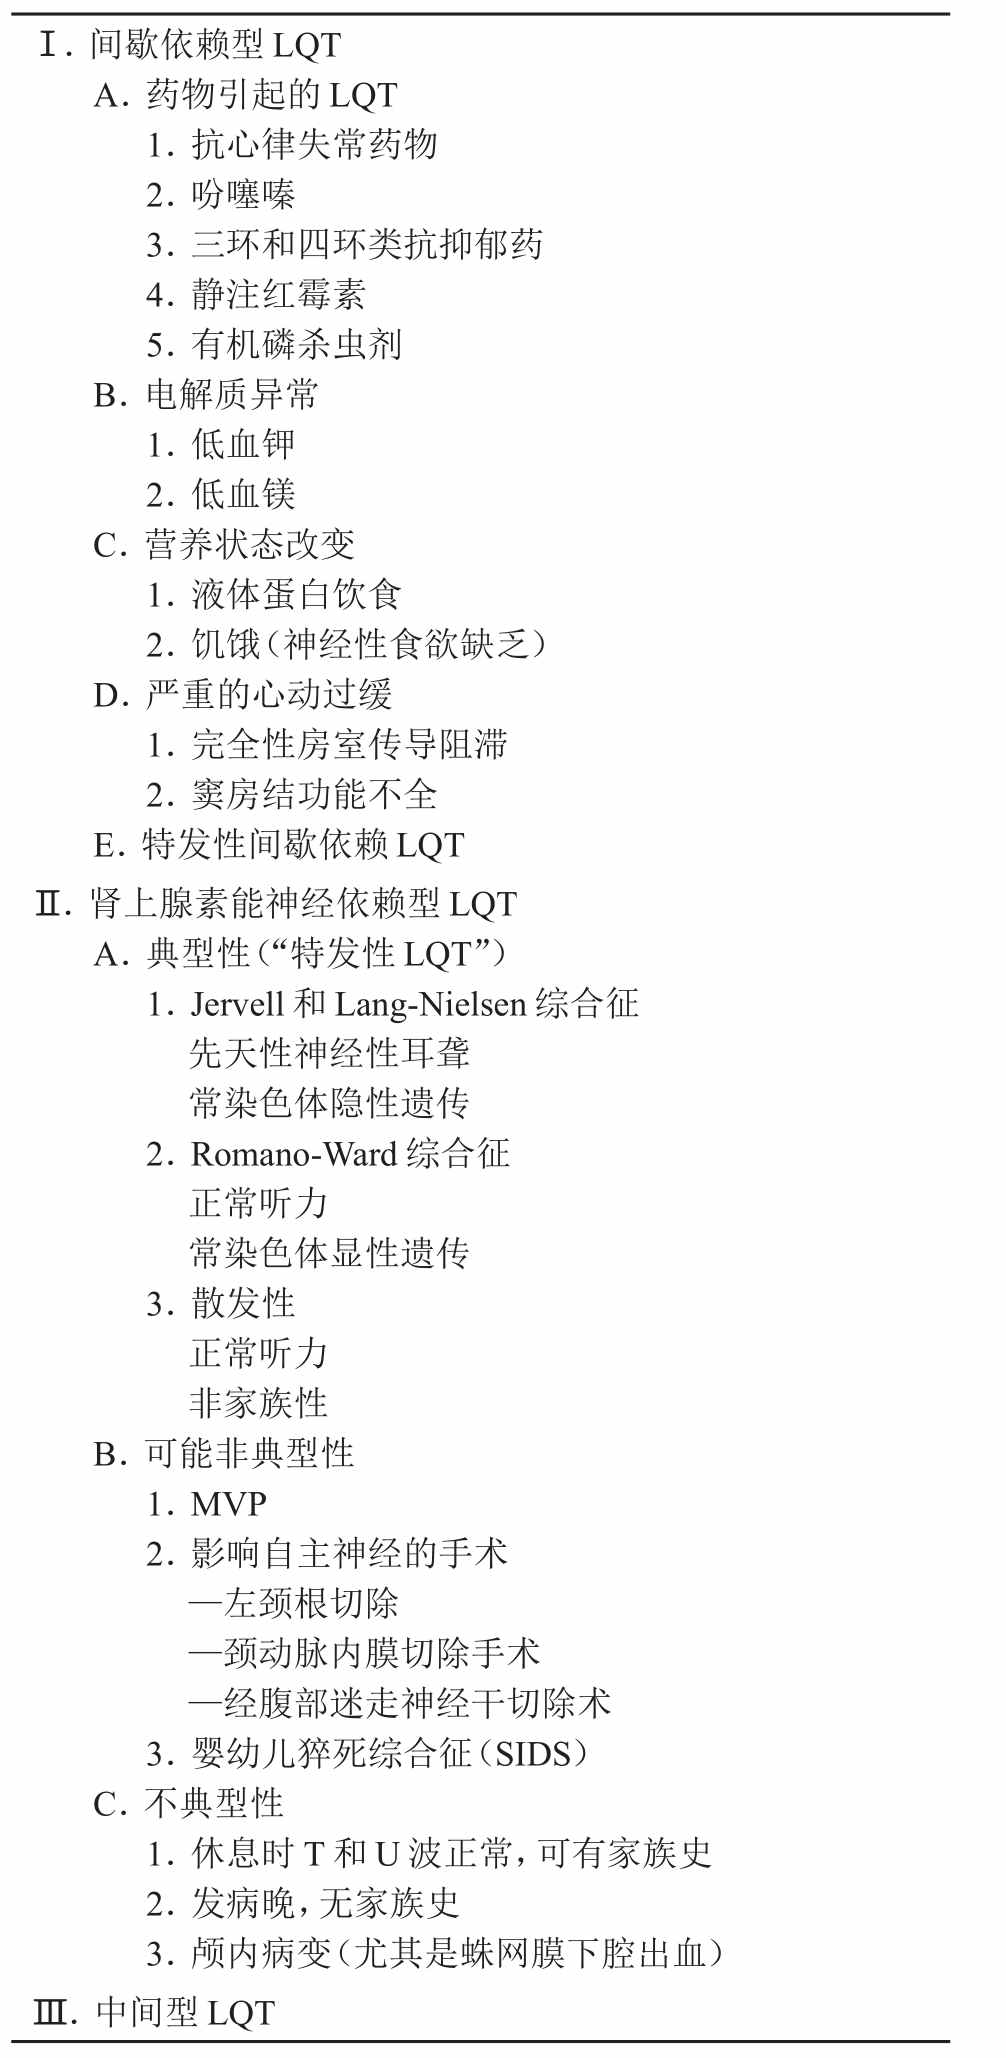
\includegraphics[width=3.34375in,height=6.85417in]{./images/Image00444.jpg}
\end{table}

\subsubsection{LQTS并发TdP的机制}

目前对LQTS时TdP的发生机制有了较深认识。上述基因突变导致离子通道功能障碍,使复极时间和动作电位时间延长,心室跨内、中、外3层肌细胞复极离散度及心室壁不同部位复极离散度均显著增加,产生后除极及触发活动,同时也是形成折返的基础。临床及实验研究结果显示:LQT\textsubscript{2}
、LQT\textsubscript{3}
发生TdP的机制是早期后除极(EAD)及触发活动,而TdP的维持则可能是由反复的EAD及触发活动和折返共同参与的。实验研究显示,LQT\textsubscript{1}
模型只有在β肾上腺素刺激下才发生TdP。目前认为,LQTS时TdP的发生机制可能是后除极及触发活动;而TdP的维持则需反复的触发活动和(或)折返激动。

\subsection{诊断}

\subsubsection{临床表现特点}

扭转型室速常表现为反复而短暂的发作,由于发作时心室率极快,心排血量锐减,常引起眩晕或晕厥;发作时间较长可引起抽搐及一系列脑缺氧表现,晕厥时间与心动过速发作时间相一致;而一般室速频率通常较慢,因此较易耐受,有时也可伴有晕厥,但与前者不同,晕厥常发生在心动过速的开始,以后尽管心动过速依然存在,晕厥可消失。扭转型室速如未能及时得到控制,可不断反复发作,最后转为心室颤动而死亡。

\subsubsection{间歇依赖性LQTS}

TdP发生于显著的心动过缓、期前收缩及房颤的长R-R间距和阵发性心动过速终止的长间歇后,故名。可能发生此型TdP的高危患者为:有TdP发作史,器质性心脏病心动过缓,应用可延长QT间期的药物,低钾或低镁血症等。

\paragraph{TdP发作前的心电图}

基础心律可为正常窦性心律,也可为缓慢性心律失常,如窦性心动过缓、交界区心律、高度或完全性AVB等,有时也可为心房颤动或其他异位心律。这些基础心律的心电图特征均有明显的QT或QU间期延长(QT间期≥0.6秒为将发生TdP的高危指标,但约1/5TdP发作前的QT间期<
0.5秒,而胺碘酮服用者QT间期> 0.6秒时发作TdP者<
1\%);同时伴有T波增宽、平坦、高大或深倒置,U波也可呈宽大、多形等改变;室速常由一伴较长联律间期的室性期前收缩(室早)所诱发,其联律间期(距)常在0.5~0.7秒之间,室性期前收缩可频繁发生,呈RonT现象。约95\%的患者,发作前最后一个室上性心搏有长R-R间期(长周期),促发TdP的室性期前收缩落在前一室上性或窦性搏动延长的T波上(短周期),形成了特殊的“短-长-短”室速模式。

\paragraph{TdP发作时的心电图}

TdP发作时的心电图呈现一系列形态增宽的心室波群,其频率在200~250次/分,平均约为220次/分,节律不甚规则,心室波群的极性及振幅呈时相性变化,每隔5~20个心动周期,QRS波的尖端即逐渐或突然倒转其方向,形成了围绕基线QRS波上下扭转的形态(图\ref{fig102-11})。上述室速波形的扭转形态不一定在所有导联中均能见到,因此,最好能采用多导联同步描记以显示此种现象。每次心动过速发作时间为数秒至数十秒,可自行终止,但极易复发。如不及时治疗,此种反复发作过程可持续并进展为室颤。

\subsubsection{肾上腺素能依赖性LQTS}

为特发性或家族性LQTS。虽非多见,却具有非冠状动脉性、与遗传有关的、以交感神经为中介的猝死倾向,为一家族遗传性疾病,可分为3类(参见表\ref{tab102-12})。多发于儿童,常于运动、应激(惊吓)、情绪激动或交感兴奋药应用时发作,呈肾上腺素能依赖性。常表现为短暂发作的眩晕、晕厥、抽搐及其他脑缺氧症状,可蜕变为室颤而死亡。

TdP发作前心电图为QT间期进行性延长,T波在发作前数秒至数分钟呈周期性改变,U波振幅逐渐增大,达“阈值”后触发TdP(图\ref{fig102-12}),发作时心电图与间歇依赖性LQTS相似。

\begin{figure}[!htbp]
 \centering
 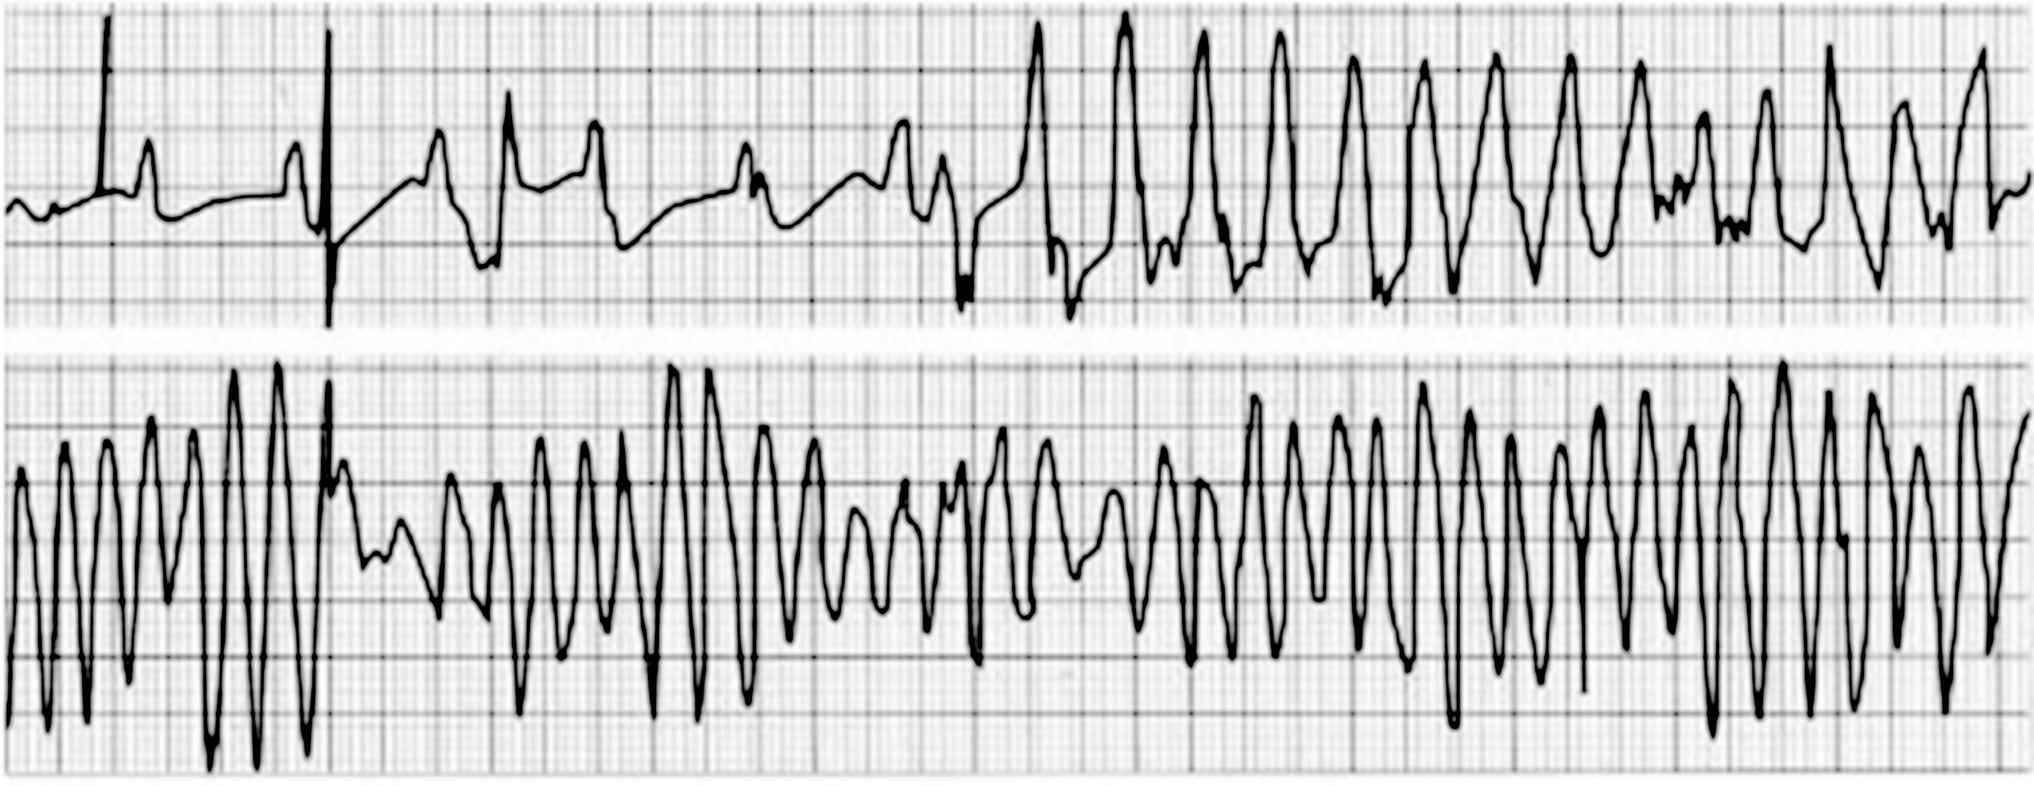
\includegraphics[width=5.89583in,height=2.28125in]{./images/Image00445.jpg}
 \captionsetup{justification=centering}
 \caption{患者女性,49岁,三度AVB,QTc为0.67秒,发生典型的TdP}
 \label{fig102-11}
  \end{figure} 

\begin{figure}[!htbp]
 \centering
 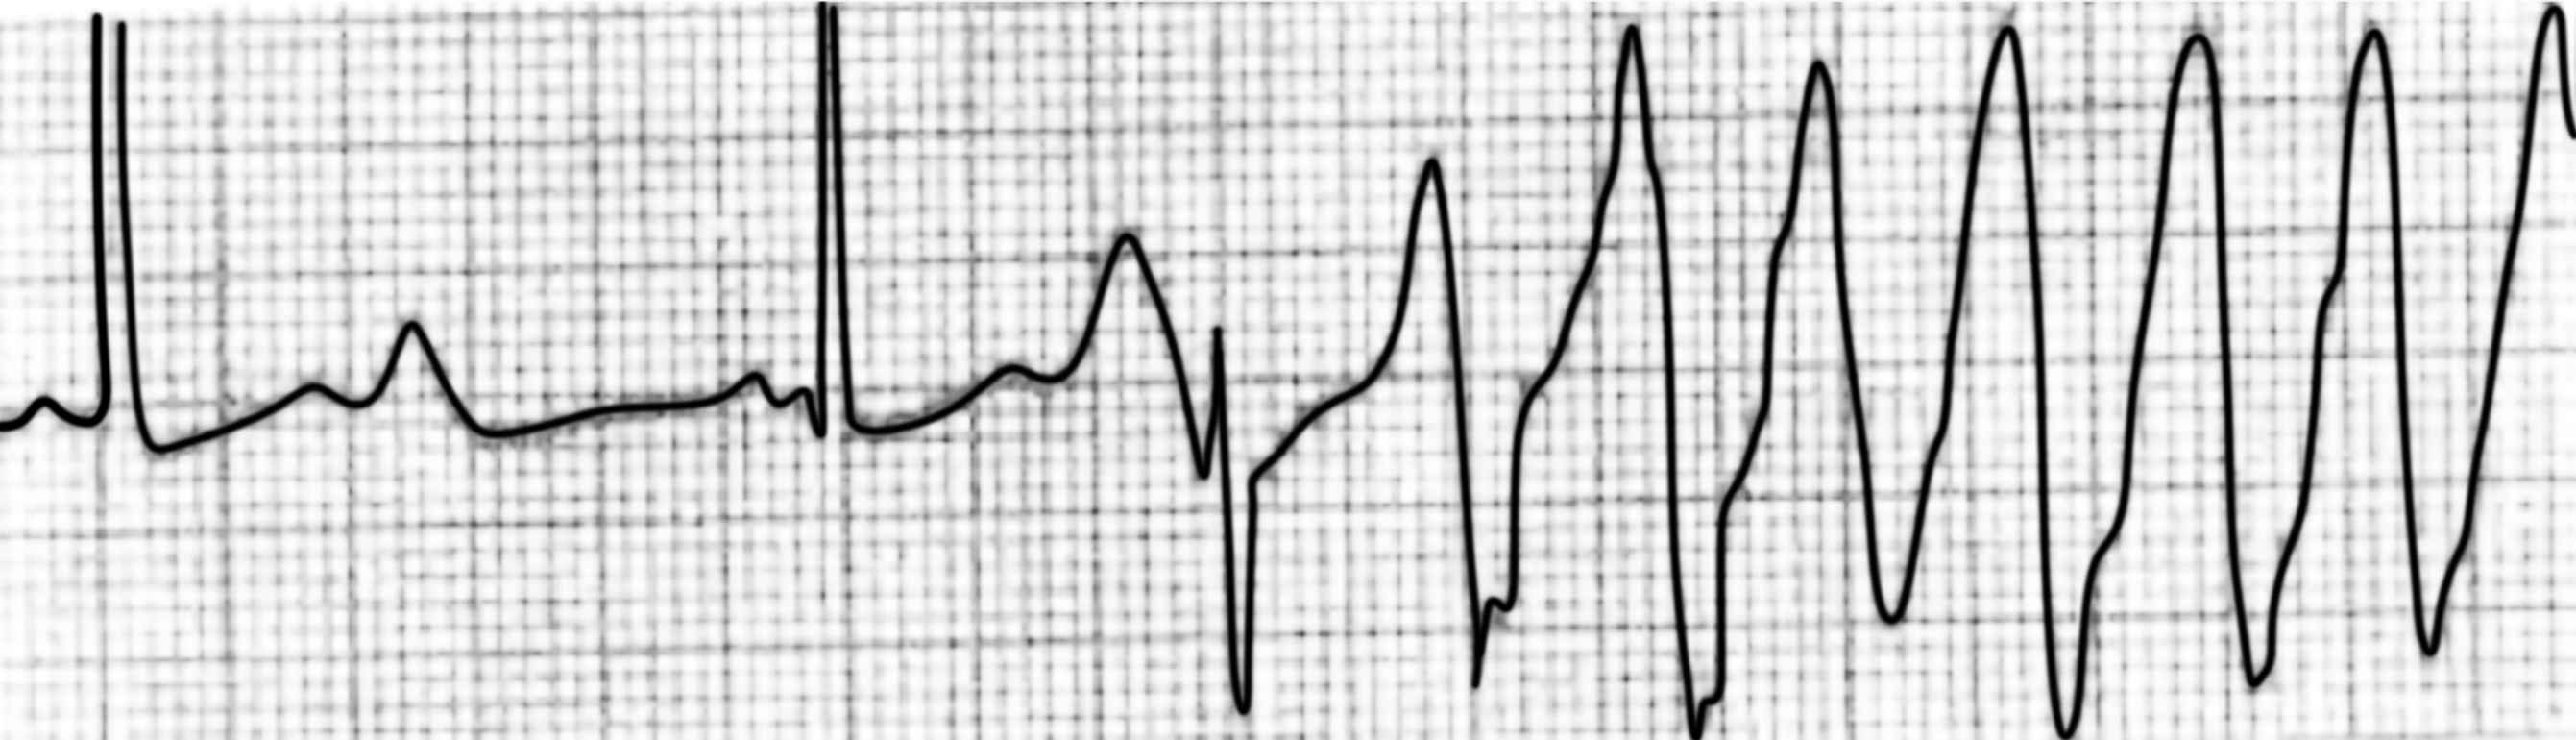
\includegraphics[width=5.89583in,height=1.6875in]{./images/Image00446.jpg}
 \captionsetup{justification=centering}
 \caption{肾上腺素能依赖性扭转型室速}
 \label{fig102-12}
  \end{figure} 

第一和第二心搏的 T波交替改变,一晚发期前收缩落于Tu波降支诱发TdP

特发性LQTS的诊断标准(1993年)见表\ref{tab102-13}。

非典型性LQTS患者常无家族史,多发于老年,临床表现较轻,休息时U波正常或接近正常,可于运动和精神紧张时U波增大,发生室速、晕厥甚至猝死。运动试验或Ⅰa类抗心律失常药物亦可诱发。二尖瓣脱垂者表现为肾上腺素能依赖性LQTS发作前常无间歇。蛛网膜下腔出血和颅内出血的TdP起始长间歇可有可无,常表现为QT明显延长,T波高大增宽及明显U波。

\begin{table}[htbp]
\centering
\caption{1993年LQTS诊断标准}
\label{tab102-13}
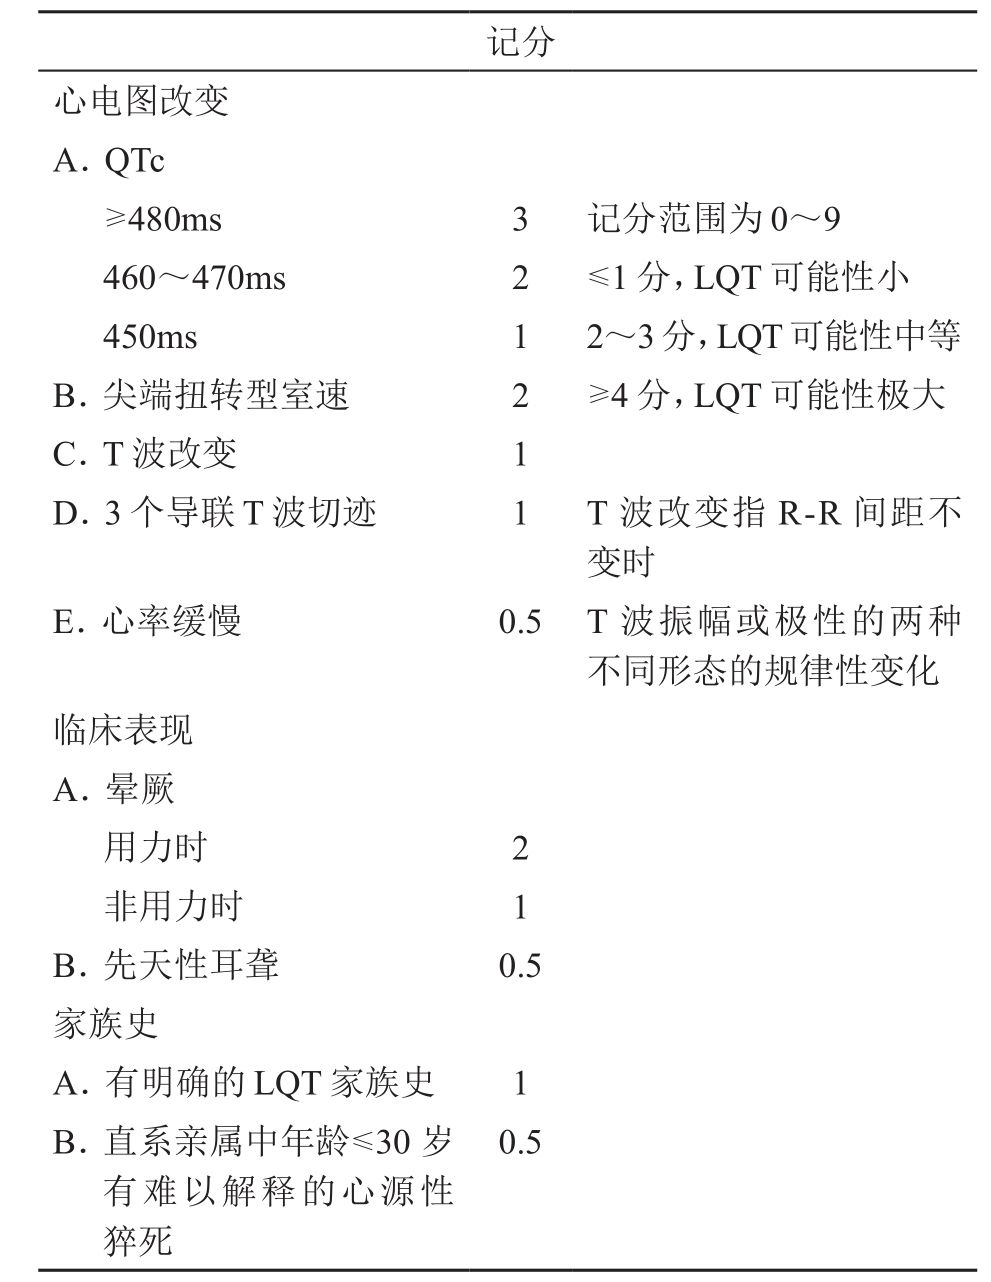
\includegraphics[width=3.29167in,height=4.26042in]{./images/Image00447.jpg}
\end{table}

\subsubsection{中间型TdP}

患者的心跳长间歇或肾上腺素能兴奋均可致TdP发生,部分患者心电图有明显U波;重体力负荷或情绪激动、无长间歇亦可发生TdP。

\subsubsection{诊断注意事项}

正常人经心率校正后QT间期(Q-Tc)的上限为0.40秒,当Q-Tc大于0.40秒时即为QT间期延长,又称为复极延迟。TdP与心室的复极延迟和不均一有关,其中QT间期延长是导致TdP的主要原因之一,因此将QT间期延长并伴有反复发生的TdP称为长QT综合征(LQTS)。据此,发作间期心电图示QT间期延长是诊断TdP的必备条件。典型TdP的诊断并不困难。TdP发作时的心电图尚须与一般室速或心室颤动相鉴别:一般室速表现为一系列形态几乎恒定的宽大QRS波群,ST段与T波可以辨认,发作往往不会自行终止;一般室速也可有RonT室性期前收缩(室早)诱发,但室性期前收缩联律间期较短。心室颤动时无法识别波群及ST段与T波,发作持续即死亡。此外,尚需与具有“尖端扭转”形态,但QT间期正常的多形性室速鉴别,详见本章第5节“室性心动过速”部分。

\subsection{治疗}

TdP是恶性快速性室性心律失常类型之一,如能及时、正确治疗,发作可以得到控制,如能进一步消除或治疗病因,可使之痊愈。不同类型的TdP,由于病因学基础不同,在治疗上有一定区别,现分述如下:

\subsubsection{间歇依赖性TdP的治疗}

\paragraph{纠正或解除病因与诱因}

包括停用诱发QT间期延长的药物,纠正电解质紊乱,治疗明显的心动过缓等。

\paragraph{提高基础心率}

凡使心率提高的方法均可使心室复极离散度缩小。可用心房或心室调搏(使心室率≥110
次/分),或用异丙肾上腺素静脉滴注或阿托品注射(使心室率> 100次/分)。

\hypertarget{text00293.htmlux5cux23CHP10-2-6-1-3-1-2-1}{}
(1) 调搏或经静脉起搏治疗:

在房室传导正常的患者,以心房调搏最好,可最大程度地减少心室复极差异,缩短QT间期。起搏/调搏目的是提高基本心率,不是用超速起搏治疗室速本身。本治疗一般需持续至病因纠正后,起搏频率应逐渐降至可预防室性期前收缩前的频率。

\hypertarget{text00293.htmlux5cux23CHP10-2-6-1-3-1-2-2}{}
(2) 异丙肾上腺素:

可缩短QT间期及提高基础心率,心室复极差异减少。符合以下条件时方可使用本药:①TdP确切是由获得性LQTS引起的;②有相应的心动过缓;③TdP是间歇依赖性的;④心脏起搏不能立即实施。可用静脉滴注方法,调节其剂量使心室率维持在90~110次/分之间。此法简单易行,但必须严密观察,随时调节频率。有心肌缺血及高血压患者为相对禁忌证。阿托品有类似作用,但疗效差,也不宜持续应用。

\paragraph{静脉补钾和补镁}

钾离子与复极过程密切有关,低钾可使细胞膜对钾的通透性降低,使复极延迟。通常用氯化钾静滴方式给予,钾盐总量需根据缺钾程度而定。Mg\textsuperscript{2+}
通过阻断Ca\textsuperscript{2+}
内流,降低LQTS患者早期后除极的振幅至阈值下,从而抑制触发性心律失常发生,是短期内抑制TdP再发的有效药物,也是治疗获得性和特发性LQTS扭转型室速的首选药物。出现TdP的患者,无论是否存在低镁,均应静脉应用镁剂。临床以2g硫酸镁溶于20ml溶液中静脉注射,多数患者在注射过程中有“面部潮红”现象,症状的轻重取决于注射速度。对无症状的室性期前收缩二联律者(即将发生TdP)注射速度要慢(1g/min);对TdP正在发作的患者注射速度要快(2g/30~60s),可隔5~15分钟重复1次,也可以3~10mg/min持续静脉点滴。大剂量或肾功能不全时,随着血镁浓度的升高,会出现低血压、昏睡、以致心搏骤停。镁可使原已存在的房室传导阻滞或低血压恶化。膝反射消失是镁中毒的信号。补镁的同时必须补充足够的钾,使血钾水平>
4.5mmol/L。

\paragraph{其他措施}

①禁用Ⅰa、Ⅰc和Ⅲ类抗心律失常药,可试用Ⅰb类,如利多卡因静脉注射,但其对TdP的有效率只有50\%。②扭转型室速持续发作时,应按心脏骤停原则治疗,包括胸外按压、人工呼吸等,有室颤倾向者,可用低能量电复律。由于电击本身可使心肌钾丢失,使发作加重,故应积极预防其发作,避免反复电击。③对顽固发作且用药矛盾的严重心动过缓、严重传导障碍者,宜安装永久调搏器。

\subsubsection{肾上腺素能依赖性LQTS}

TdP发作时静脉注射镁剂,用量与方法见上述。

1.β受体阻滞剂
为防治肾上腺素能依赖性LQTS的最主要药物,以普萘洛尔为最常用,剂量可用2mg(/kg•d),必要时增加剂量。β阻滞剂可引起心率减慢,从而使QT间期延长,但QTc可能缩短。经持续足量β阻滞剂治疗后,可使特发性LQTS有症状而未治疗者的死亡率由78\%降至6\%左右。

获得性和先天性LQTS具有相似的病理生理学基础,它们都是钾外流的阻滞所致。在获得性LQTS患者,异丙肾上腺素可提高心率,预防TdP的复发;而在先天性LQTS患者,允许长期服用β受体阻滞剂,治疗上如此矛盾,令人费解。一个可能的解释是,异丙肾上腺素可使外向钾电流和内向钙电流都增加,在正常或Ikr被阻滞(快速激活延迟整流钾电流,多数获得性LQTS都是该电流受阻)的情况下,外向钾电流的增加占优势,所以导致的最终结果是净外向电流的增加和复极缩短。另一方面,当Iks被阻滞(缓慢激活延迟整流钾电流受阻,遗传性LQTS的主要形式)时,肾上腺素能激动引起很小的外向钾电流增加和相对大的内向钙电流增加,结果异丙肾上腺素会延长复极、促发EAD。

2.患者应避免剧烈体力活动及精神刺激 ,禁用延长心室复极和儿茶酚胺类药物。

3.经过用 β阻滞剂治疗仍有晕厥发作,需进行左侧颈胸交感神经节切除术(left
cervicothoracic
sympathectomy,LCTS)。某些患者手术后仍需用β阻滞剂治疗,但剂量可减少。治疗效果以长期随访不再有晕厥发作来衡量,而QT间期可能并不明显缩短。

4.对经上述治疗仍有晕厥发作者
,可试用以下药物:维拉帕米可能通过影响后除极化而发挥作用,但长期口服的效果尚不清楚;扑米酮对预防发作可能有效;苯妥英钠、洋地黄,它们可缩短QT间期,但不一定能防止晕厥发作。有关先天性和(或)获得性LQTS的治疗选择见表\ref{tab102-14}。

\begin{table}[htbp]
\centering
\caption{先天性和(或)获得性LQTS的治疗选择}
\label{tab102-14}
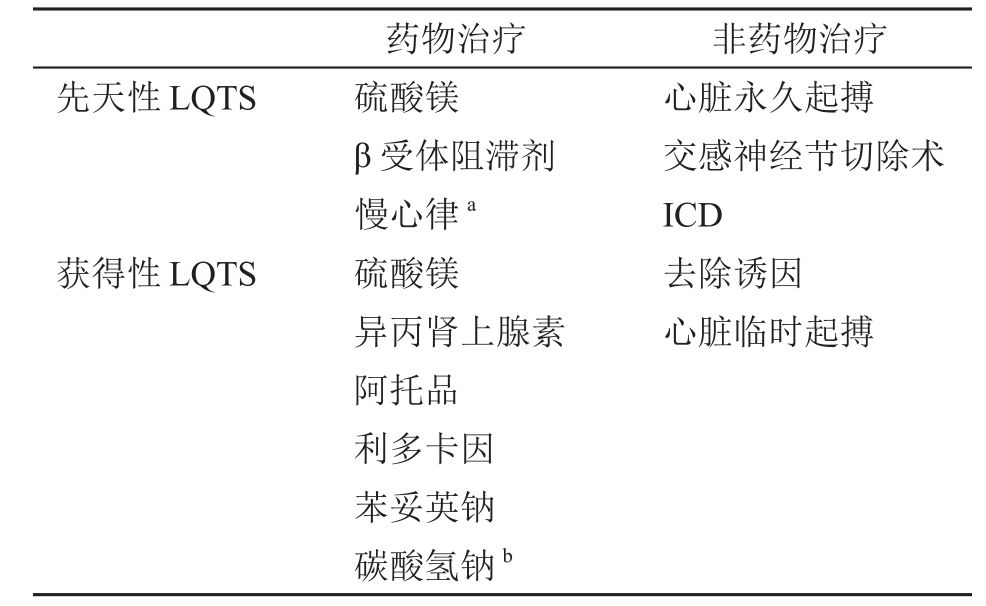
\includegraphics[width=3.27083in,height=2.01042in]{./images/Image00448.jpg}
\end{table}

\textsuperscript{a} 针对SCN5A基因突变诱导的TdP;\textsuperscript{b}
针对奎尼丁引起的TdP

5.其他
①Ⅰa类药物对二尖瓣脱垂并TdP可能有效;普萘洛尔或阻滞左侧星状神经节药物可抑制蛛网膜下腔出血和颅内出血的TdP。②持续发作药物治疗无效时可行电复律。③有条件时可植入埋藏式自动复律除颤器(ICD)。

\subsubsection{中间型的治疗}

如发作兼有上述两型特征时,可应用β阻滞剂而不用异丙肾上腺素;可安装永久性起搏器但疗效尚不肯定。

\hypertarget{text00293.htmlux5cux23CHP10-2-6-2}{}
特发性室性心动过速

特发性室性心动过速(idiopathic ventricular
tachycardia),亦称“良性室速”,约占室速总病例数10\%。1922年由Gallara首次描述,当时称之为“礼炮样室速”,为临床、心电图和电生理均具特征的临床实体,心脏及解剖功能正常,统称为特发性室速。其中某些患者对维拉帕米治疗有效,称为维拉帕米敏感性室速;若运动或儿茶酚胺诱发称为运动诱发或儿茶酚胺敏感性室速;如源于左心室心尖下部或前上方称为特发性左心室室速(idiopathic
left ventricular
tachycardia);源于右室流出道室间隔者称为右心室室速(right ventricular
tachycardia)。

\subsection{病因与发病机制}

特发性室速发生于无任何病理改变的心脏(亦称为原发性电疾患,primary
electrical
disease),或实质为一类亚临床型各种检测方法均难以发现的器质性心脏病,如小灶性心肌炎、局限性心肌纤维化、原发性扩张或肥厚性心肌病、二尖瓣脱垂、隐匿型冠心病、小右室室壁瘤或轻度右室发育不全、“运动员心脏”等。

现多将发病机制归于:①折返机制:发作时QRS波群呈RBBB伴电轴左偏者,折返环位于左后分支普肯耶纤维网内;RBBB伴电轴右偏者,源于左心室心尖前上方;LBBB伴电轴正常或右偏者,源于右室流出道间隔。常无“温醒”(warm
up)现象,程控刺激可诱发或终止。②触发活动:某些维拉帕米敏感性室速的病理机制与此有关。③原发性电激动障碍:心肌细胞代谢或生化功能原发性缺陷。

\subsection{诊断}

本型VT的共同临床特点是:多为中青年患者,室速反复发作。患者可能完全无或只有轻度心悸、胸闷,但晕厥、心搏骤停少见;很少发展为器质性心脏病;心脏物理检查、心电图、运动负荷试验、超声心动图、核素心血管造影及心导管检查等均属正常。

临床表现方面可分为以下两型:

\paragraph{反复的单形性室速(RMVT)}

亦称“右室室速”,约占本型的70\%,多源于右室流出道,也可见于其他部位,为介于单纯室性期前收缩与持续性室速间的一个类型,机制与延迟后除极引起触发活动有关。非发作期单发室性期前收缩或成对室性期前收缩,短阵室速波形与右室室速发作时波形相同。QRS波宽0.13~0.14秒,持续5~20个心搏,心室率110~160次/分,可自行终止。最常见为LBBB伴电轴右偏或正常,Ⅱ、Ⅲ、V\textsubscript{6}
导联QRS波形向上,额面电轴向下;亦可为RBBB伴电轴右或左偏;可由运动或静滴异丙肾上腺素诱发,但不易为程序刺激诱发。维拉帕米不但可控制室速急性发作而且能预防其复发。

\paragraph{持续性室速}

占特发性室速的30\%,亦称“特发性左室室速”或“分支阻滞型室速”,机制与cAMP介导的触发活动或折返有关。无室早或室早二联律发生,发作时间可长达数日,不易转为窦性心律。常见RBBB型伴电轴左偏,V\textsubscript{1}
导联呈RBBB,Ⅱ、Ⅲ、aVF为左前分支阻滞,偶为RBBB型伴电轴右偏;QRS波群正常或稍增宽,不易为异丙肾上腺素诱发,多为程控期前收缩诱发或终止。静注维拉帕米可终止发作而口服维持则可预防此型室速发作(亦称维拉帕米敏感性室速),β受体阻滞剂虽可减慢室率但少有终止或预防效果。

\subsection{治疗}

首选药物为维拉帕米:急性发作时用维拉帕米静注,口服用于预防发作。胺碘酮、普罗帕酮、普鲁卡因胺、氟卡尼可能有效。对持续性室速亦可用消融治疗。

\hypertarget{text00293.htmlux5cux23CHP10-2-6-2-4}{}
参 考 文 献

1. Drew BJ,Ackerman MJ,Funk M,et al. Prevention of torsade de pointes
in hospital settings:a scientific statement from the American Heart
Association and the American College of Cardiology Foundation.
Circulation,2010,121(8):1047-1060

2. Kramer DB,Zimetbaum PJ. Long-QT syndrome. Cardiol
Rev,2011,19(5):217-225

3. Kannankeril P,Roden DM,Darbar D. Drug-induced long QT syndrome.
Pharmacol Rev,2010,62(4):760-781

4. 陈灏珠 ,林果为.实用内科学.第13版.北京:人民卫生出版社,2009:1438

\protect\hypertarget{text00294.html}{}{}

\section{预激综合征伴快速性心律失常}

预激综合征(pre-excitation
syndrome)或WPW(Wolff-Parkinson-White)综合征,简称预激,是指患者除了正常的房室传导通路外,还有先天的附加房室传导通道(旁路),引起心电图异常伴心动过速倾向的临床综合征。诊断主要靠心电图。WPW综合征其实是一种并不罕见的心律失常,在西方国家的发病率约为0.1\%~0.48\%,而在国内约为0.44\%~0.68\%。WPW综合征可见于任何年龄,男性多见(约占60\%~70\%),且患者大多无器质性心脏病,其本身并不产生血流动力学障碍和临床症状,多在心电图常规检查中偶然发现,或因并发心动过速就诊。约有40\%~80\%的人易并发各种心律失常,其中以室上性心动过速最为常见,其次为房颤及房扑,偶有心室颤动。WPW综合征并发快速性心律失常为心血管病急症,在诊断与治疗上均有其特殊性,及时正确诊断和处理具有极其重要的临床意义。

\subsection{病因与发病机制}

\subsubsection{病因}

分子遗传学研究表明,WPW综合征包括家族性和散发性,以散发性为主,家族性WPW综合征为一种常染色体显性遗传病。

患者大多无器质性心脏病,少数有先天性或后天性心脏病。在先天性心脏病的患者中尤以Ebstein畸形最常见,其发生WPW综合征的概率为5\%~25\%,且均是右心房室旁路。在室间隔缺损和大血管转位者伴有WPW综合征的机会也比自然概率高。二尖瓣脱垂患者伴有WPW综合征者较多,且多为左侧房室旁路。也有家族性倾向的报道。

\subsubsection{解剖生理学基础}

WPW综合征的基本解剖-生理学基础是心房和心室之间存在单条或多条异常的传导组织---附加旁路(accessory
pathway,AP),其电生理学特点为具有传导性。通常AP的传导为双向性,即可前向传导(从心房传至心室)和逆向传导(从心室传至心房)。由于AP缺乏房室交界区的生理“延搁”作用,故其传导速度快,心房冲动部分经AP快速下传,提前到达AP的心室端,激动邻近心肌,从而造成心室提前激动和改变心室肌正常兴奋顺序,其结果是心电图上QRS波群畸形,起始部分有预激波(delta波);心房冲动的其余部分可沿正常房室传导途径下传,与AP引起的心室激动合并形成心室融合波。心室融合波的形成由正常房室传导通道与AP的不应期长短决定:正常通路不应期长,或冲动大部沿AP传导,则QRS畸形明显;AP不应期长,则心室融合波接近正常。已知的AP有下列几种,同一患者可有多条AP:

\paragraph{房室旁路(Kent束)}

Kent束是经房室环直接连接心房和心室的AP,大多位于左、右两侧房室沟或间隔旁。由其引起的预激为典型预激综合征。本型最常见。其心电图特征为:①P-R间期<
0.12秒,大多为0.1秒,P波正常;②QRS时限≥0.11秒;③QRS波群起始部粗钝,与其余部分形成顿挫,即所谓预激波或δ波(delta波);④PJ间期正常;⑤继发性ST-T波改变。此心电图改变尚可分为A、B两型。A型预激:预激波和QRS波群在V\textsubscript{1}
导联均向上,提示左室或右室后底部心肌预激;B型V\textsubscript{1}
导联的预激波和QRS波群的主波则均向下,提示右室前侧壁心肌预激。

\paragraph{房希旁路(James束)}

James束是后结间束绕过房室结的上、中部而终止于结下部或直达希氏束,造成房室之间的传导短路。终止于房室结下部者,称为James束不完全型;终止于希氏束者,称为James束完全型。此型预激称为变异型预激综合征,或LGL(Lown-Ganong-Levine)综合征。本型少见。其心电图特征为:①P-R间期<
0.12秒;②QRS波群时间正常;③无预激波。故又称短PR、正常QRS综合征。

\paragraph{结室(或结束)旁路和束室旁路(Mahaim束)}

前者连接房室结与心室或右束支,后者连接希氏束与心室。其心电图特征为:①PR间期正常(≥0.12秒);②QRS波群起始部有δ波,但δ波小;③QRS波群时间≥0.11秒,但增宽轻微。

\paragraph{房束旁路(Mahaim束)}

连接心房与远端右束支或右室心尖部。其心电图特征为:PR间期正常;QRS波形态正常;无预激波。

几种特殊类型的预激综合征:

根据房室旁路前传的有效不应期、传导速度及其房室结传导特性的不同,临床上WPW综合征可有多种表现形式,如完全性、隐匿性、潜在性、间歇性、获得性、手风琴效应及多旁道预激等。

1.完全性预激
发生机制与典型WPW综合征相似,只是心房激动全部经AP下传心室。心电图特点是:①P-R间期缩短;②QRS间期增宽>
0.14秒(甚至>
0.20秒),δ波可不明显,但QRS波群起始和终末部均模糊、顿挫;③PJ间期延长;④伴有显著ST-T改变。

2.隐匿性预激(concealed pre-excitation)
AP若存在单向阻滞,激动只能逆向传导,临床上虽有折返性心律失常,但常规心电图不能显现。原因有:①AP存在前向性阻滞;②AP正向传导不应期长;③心室肌电位高于心房肌。如激动经AP传入心房时正值心房易损期可导致心房颤动。其特点有:①有频发或顽固性室上性心动过速史;②窦性心律加快时,即使无房性期前收缩,也可自动诱发反复心律或室上速;③心动过速时,Ⅱ、Ⅲ、aVF导联QRS波之后可见P\textsuperscript{−}
波,且R-P\textsuperscript{−} <
P-R;④心动过速伴旁道同侧功能性束支传导阻滞(BBB)时,心率减慢;⑤房室反复性心动过速可伴有心房扑动或心房颤动;⑥用维拉帕米治疗时,在心动过速终止前可见较为固定的长-短周期交替出现。

3.潜在性预激
指AP有前传能力但患者平时体表心电图无明显预激表现,只有在食管调搏或电生理检查心房程序刺激或使用兴奋迷走神经方法或钙离子拮抗剂阻断正常房室传导时,方可显示明显的预激心电图表现,称为潜在性预激。其原因可能与下列因素有关:①房室结传导加速,心房激动经房室结-希氏束径路传导与经AP前向传导几乎同时到达心室;②经AP前向传导时间长(AP传导速度慢)或从窦房结到达AP的距离远,则心室预激成分极小;③两条AP位于相对位置上,产生相反的δ向量,使心电图上δ波互相抵消。

4.间歇性预激
为典型预激与不典型预激的不连续性交替,约47\%的显性预激存在间歇性改变,其机制与普通预激基本相同,只是间歇性预激的AP在一定条件下才有传导作用。原因有:①运动试验可让半数WPW者心电图正常化;②迷走神经张力高对房室结的传导有抑制作用,可使δ波增大;③AP位于左侧;④AP前传不应期长,易使预激程度减少或无预激表现;⑤房内传导时间愈长,预激程度愈少;⑥起搏点位置;⑦旁道内隐匿传导;⑧多旁道的影响。每次正常激动后出现一次预激现象,称为交替性预激,易被误诊为室性期前收缩二联律。

5.获得性预激
发生在风湿热、急性心梗、冠心病或高血压等疾病之后称为后天获得性WPW。其机制可能由于正常房室结因疾病使传导性降低甚至遭到破坏,因而心房激动的一部分或全部通过AP下传心室。实际上异常通道原来就存在,AP多数有逆向传导功能。

6.手风琴效应(预激程度不等的WPW)
在每次窦性激动中,心房激动经房室正道和AP下传比例逐渐变化。心电图表现为P-R间期长短不等,δ波的明显程度亦不等。对应于P-R间期从短到长,δ波从明显到不明显乃至消失。这种周期性变化如同手风琴的伸缩,称为“手风琴效应”。

7.多旁路预激
通常WPW患者只有一条AP,心电图检查为同一表现。少数患者存在两条或多条AP,平时激动沿速度快、不应期短的AP下传,仅显示单旁道预激图形;当心率发生明显变化时,其余AP也可显示活性,出现另一预激旁道的表现,则同一患者A型、B型预激交替出现。

\subsubsection{WPW合并室上性心动过速}

阵发性室上速是WPW并发的最常见快速心律失常。根据其折返环路可分为:

\hypertarget{text00294.htmlux5cux23CHP10-2-7-1-3-1}{}
(一) 顺向型房室反复性心动过速(OAVRT)

顺向型房室反复性心动过速(orthodromic atrialventricular reciprocating
tachycardia,OAVRT),即顺向型房室折返性心动过速,在有症状性WPW患者中发生率约84\%。在大多数情况下,AP的前向性有效不应期(AERPAP)比正常房室通道长,而AP的逆行性有效不应期却比正常房室通道短,故房性冲动总是沿正常房室传导系统前向传导,沿AP逆行传导,形成由心房→房室结(AVN)→希-普系统(HPS)→心室→AP→心房的大折返环路。倘若冲动在此折返环路中继续传导下去,则形成OAVRT。

OAVRT的发生机制有多种,可由心房、心室或交界性期前收缩引起,但以室性期前收缩最多见。由于房室结存在单向阻滞特性,室性期前收缩在房室结内逆行传导受阻,期前收缩冲动沿AP逆传激动心房,然后,再进入房室结、希-普系统(HPS)前向传导激动心室,形成大折返性心动过速。某些WPW患者,房性期前收缩亦可诱发OAVRT,但必须具备:①AP前向不应期比正常通道长;②房性期前收缩必须足够早。这样期前收缩冲动不能经AP下传,只循正常房室通道前向传导激动心室,产生正常QRS波,倘若此时AP不应期已过,则冲动沿AP逆传至心房,并再进入房室结、希-普系统,建立大折返性心动过速。有时,当窦性心律或心房率增快时亦可诱发OAVRT:由于自主神经张力的波动,致使AP和房室通道的传导速度发生分离而产生折返;同时,在窦性心律加速时,隐性AP的逆行有效不应期随心动周期缩短而缩短,更易逆行传导激动心房,并再次进入房室传导系统,建立大折返性心动过速,多见于左侧房室AP的患者。不论哪种形式诱发的OAVRT,倘若折返环路任何部位发生阻滞,则心动过速必终止,但多伴随房室传导阻滞而终止,在心电图上表现为心动过速最后1个QRS波后有逆行P′波但无QRS波。

此型室上速的电生理特征有:①V-A <
A-V,呈明显偏心性逆传;左室游离壁旁路A波最先见于冠状窦远端;右房A波明显领先为右侧旁路;中间隔旁路逆传时希氏束最先激动;②心房或心室刺激可诱发或终止心动过速。③心室刺激时不发生递减传导。④心室起搏逆传入心房,可致A-A间距缩短。⑤旁路同侧功能束支阻滞时,V-A间期延长>
20ms。

\hypertarget{text00294.htmlux5cux23CHP10-2-7-1-3-2}{}
(二) 逆向型房室反复性心动过速

逆向型或预激性房室反复性心动过速(antidromic or preexcited atrial
ventricular reciprocating
tachycardia,AAVRT),即逆向型房室折返性心动过速,少见。反复性心动过速通过AP前向传导,由正常房室传导系统逆向传导形成大折返性心动过速,谓之AAVRT。产生此种折返常需具备以下3个条件:①AP的前向有效不应期比房室结的短,AP的逆向传导不应期比房室结的长;②正常房室传导系统有稳定的室房传导能力;③整个折返时间超过折返环路中任何部位的最长不应期。心动过速时的折返方向为心房→AP→心室→HPS-AVN→心房(或心房→AP→心室→AP→心房,系多AP折返)。

其电生理特征有:①呈逆向激动心房顺序,冲动从房室结逆传对称地传导至右和左心房,典型AAVRT希氏束总是先除极,尔后继续逆传激动心房,故H波总在A波之前。②房室传导时间缩短。③房性期前收缩或室性期前收缩逆传入心房可终止心动过速;室早不改变心房逆行激动顺序,但改变逆传的A-A间距。④心房和心室波呈1∶1传导。

少数患者同时存在两条或两条以上旁路(AP),可同时有多个前向或逆向传导;或AP与房室结双通道共存;或房室结内折返,AP为无关者;或房室结内慢径路与AP构成折返环,快径路为无关者等。

\subsubsection{WPW合并心房颤动(Af)/心房扑动(AF)}

\paragraph{WPW合并心房颤动(Af)}

WPW并发Af的发生率约为11.5\%~39\%,显性多于隐匿性,多旁路多于单旁路。房颤多为阵发性,且反复发作,但也有持续发作者,具有一定危险性,容易导致心室颤动而发生猝死。成功消融AP
后Af发生率较前下降91\%以上,说明AP在介导Af发生中可能起重要作用。其机制可能与下列因素有关:①AP顺传:心室预激可使心室收缩提前→心室与心房收缩不协调和频繁的房室折返性心动过速(AVRT)发作→心房内压力升高→心房易损性增大:心房有效不应期缩短、传导减缓,增加了心房的电不稳定性。这可能是显性旁道比隐匿性旁道更易发生心房颤动的原因。②AP逆传:逆传激动若遇心房易损期或与心房内窦性(或房性)激动发生波峰碰撞(可产生波峰碎裂和扭转,易产生传导阻滞和折返),均可引起心房颤动。AP传导在Af的发生中起触发作用,但Af持续的机制(折返)与AP无关,但由于AP与正道相比具有全或无的传导和有效不应期随频率加快而缩短的特点,故AP是心房颤动顺传心室引起极快心室反应的传导径路。如果房颤发作时的R-R间期<
250ms则引起极快的心室率,导致血流动力学严重障碍,蜕变为心室扑动或心室颤动而发生猝死。

\paragraph{WPW合并心房扑动(AF)}

WPW并发AF较少见,其发生率约为4.0\%。其发生机制与Af相似。AF一旦发生,心房激动沿异常途径下传到心室,故QRS波群宽大畸形,心房激动也可沿正常途径下传,则产生正常的QRS波群。

\subsubsection{多旁路参与的折返性心动过速}

约5\%~15\%的WPW患者存在多支AP,以左后间隔与右侧游离壁AP并存最为常见。在逆向型心动过速患者,因心房颤动致心室颤动和Ebstein畸形的患者,多AP发生率特别高。有以下特点和电生理检查提示或确认存在多AP:①有晕厥发作史者;②正常窦性心律、应用抗心律失常药(如普鲁卡因胺等)、左房或右房起搏时、心房颤动时,前传δ波的改变(预激形式的改变)。③逆向心房激动多径路(室上性心动过速或心室起搏时多种逆向心房激动):逆传P波和(或)V-A间期改变;AP同侧束支阻滞时,所有部位的心房激动均未出现延缓。④顺向型心动过速发生符合预激的室性融合波。⑤由间隔AP前传,或预激心动过速周长<顺向型心动过速周长的预激心动过速。⑥不典型预激。⑦前传预激的位置和顺向型折返性心动过速时逆传心房激动最早位置不符合。⑧心电图上,约半数的多AP患者在V\textsubscript{1}
导联呈现qRs或qrS;或δ波向量与QRS电轴不在同一区域内(非一致性图形,discordant
pattern);心动过速时交替性出现两种逆向型的AVRT;或逆向型的AVRT的δ波向量与顺向型AVRT时逆传P波向量;出现不同频率的心动过速等。

\subsubsection{持续性房室交界性折返性心动过速}

持续性房室交界性折返性心动过速(permanent junctional reciprocating
tachycardia,PJRT),为好发生于房室交界区或右室右间隔旁路的所谓快-慢型折返性心动过速。此旁道纤维纤细,行走迂曲,传导速度慢,故窦性心律时无前向传导功能,无预激波。当希氏束阻断后,AP才表现为前向传导而显示预激波。其电生理学的结构基础为传导速度缓慢、具递减传导特性的隐匿性AP。常见于正常心律及窦房结功能正常的WPW者,当发生的快速心动过速终止时,常出现严重的窦性心动过缓、窦房阻滞、窦性停搏等缓慢性心律失常,引起急性脑缺血发作,临床出现晕厥、阿-斯综合征甚至猝死。

临床电生理特征有:①心动过速时室房传导时间长,靶点V-A间期>
100ms。②冠状窦口及附近为心动过速逆传最先激动部位。③心动过速时于希氏束不应期刺激心室,可提前激动心房。④心室S\textsubscript{1}
S\textsubscript{1} 刺激期周长<
300ms,室房呈递减性传导或文氏现象。⑤旁道仅具室房传导能力。⑥可由心房或心室刺激诱发或终止。

\subsubsection{WPW合并心室颤动(VF)}

WPW合并VF者,在欧美发生率为0.01\%~0.30\%,其中约81\%有Af史,引发VF的主要原因与AP有效不应期过短有关。当发生Af(或AF)及快速SVT(心室率>
200
次/分)时,快速的心房激动可通过不应期短的AP下传心室,引起极快的心室率,甚至恶化为心室颤动猝死。

\subsection{诊断}

WPW综合征实际上是心电图诊断,离开心电图检查该病的诊断是无法确立的。

\subsubsection{WPW综合征}

\paragraph{典型 WPW}

①P-R间期缩短(成人< 0.12秒,儿童<
0.10秒);②QRS波增宽(成人≥0.12秒,儿童>
0.09秒);③QRS波群起始部有δ波,导致QRS波起始部模糊、顿挫或切迹,此为预激的特征性心电图改变;④δ波常与P波融合,从而使P-R段消失;⑤P-J间期正常(<
0.26秒);⑥继发性ST-T改变:在主波向上的导联ST段上移,T波直立;在主波向下的导联ST段下移,T波倒置。

\paragraph{变异型 WPW}

\hypertarget{text00294.htmlux5cux23CHP10-2-7-2-1-2-1}{}
(1) LGL型预激:

①P-R间期≤0.11秒;②QRS波群时间正常;③没有δ波。

\hypertarget{text00294.htmlux5cux23CHP10-2-7-2-1-2-2}{}
(2) Mahaim型预激:

①P-R间期≥0.12秒;②QRS波群起始部有δ波,但δ波小;③QRS波群时间≥0.12秒,但增宽轻微。

\subsubsection{WPW并室上性心动过速}

\paragraph{OAVRT}

其特点有:①呈反复发作性,频率180~260次/分,常在200次/分以上,节律规整,QRS波群形态正常(伴束支传导阻滞或室内差异性传导时QRS波群可增宽)。②可由房性期前收缩或室性期前收缩诱发或终止。③诱发心动过速心搏常无P-R延长;逆传P′波位于QRS波群后(常在ST-T或T波上),R-P′
< P′-R,说明室房传导比房室传导要快,但在食管导联R-P′间期>
70ms(80~130ms),且房室传导为1∶1,否则心动过速即终止。④心动过速发作时常伴有QRS波电交替和(或)心动周期长短交替,同阵R-R间期差值>
30ms;心率愈快,交替现象愈明显。此种窄QRS波心动过速伴QRS波电交替对判断OAVRT具有高度特异性。推测OAVRT的电交替发生率较高的原因可能是传导系统存在解剖或功能上的差异,由于这些差异在OAVRT的快速室率时冲动传导发生交替性功能性传导延迟而发生电交替。⑤心动过速时,或出现一过性功能性束支阻滞(BBB)。旁道同侧束支功能阻滞时R-R间距或R-P′间期比原来延长35ms以上,而旁道对侧束支功能性阻滞时,则R-R间距无变化。⑥对血流动力学的影响与心室率的快慢有关。少数OAVRT可呈不典型表现。

\paragraph{AAVRT}

其特点有:①心室率常>
200次/分,δ波明显,且同于窦性心律时的δ波,QRS波群宽大畸形呈宽QRS波心动过速,不经电生理检查难与VT鉴别。②逆传P波位于QRS波群之后较远处(R-P′
> 1/2 R-R,R-P′ > P′-R,P′-R间期<
0.12秒),房室传导为1∶1,否则心动过速即终止。③常为房性期前收缩或室性期前收缩诱发,但难以为之终止。④对血流动力学的影响类同于VT。

\subsubsection{WPW合并Af/AF}

WPW合并房扑(AF)者极少见,且常为本征阵发性室上速过渡到房颤(Af)而呈短暂性出现;当然,持续性AF(数天,甚至更长时间)临床也并非罕见。当心房扑动波从AP1∶1下传时,心电图表现酷似VT,但无等电位线,Ⅱ导联扑动波较清楚,记录食管导联可显示扑动波可资鉴别。

WPW并发房颤者较多见,尤其本征引起的反复发作性或难治性室上速,以及随增龄而出现的窦房结功能减退,则更易并发Af。虽可发生于任何年龄阶段,但中老年人相对较多。WPW合并Af/AF时,因房率过快致快速心室反应,引起严重的血流动力学改变,心室率愈快,血流动力学改变愈明显。Af/AF一旦发生,快速的心房激动可经AP和AVN-HPS下传心室,其心室率的快慢及激动顺序取决于AP和AVN-HPS的前传功能状态,其大致又可分为三种类型:

\paragraph{AVN-HPS前传优势型}

常见于隐匿性、潜在性和间歇性WPW。心房激动仅能或主要经AVN-HPS下传心室,QRS波群形态以室上性为主,心室率常超过140次/分(AVN-HPS功能正常),但很少超过200次/分(除非伴有AVN加速性传导)。对血流动力学影响相对较轻。由于心动过速引起的神经体液改变,致使儿茶酚胺增加,后者可强化AP传导功能,因此部分潜在性和间歇性WPW发生Af后,可以恶化为非AVN-HPS前传优势型。

\paragraph{AP前传优势型}

该型患者AP前传能力强或因误用了AVN阻滞剂(洋地黄类、β阻滞剂、钙离子拮抗剂)使AVN-HPS前传封闭,激动仅能或主要经AP下传心室。心室率极快(>
200次/分),QRS波群呈完全预激形,极少数呈部分预激或室上形,血流动力学改变较明显,易恶化为心室颤动而危及生命(图\ref{fig102-13})。

\begin{figure}[!htbp]
 \centering
 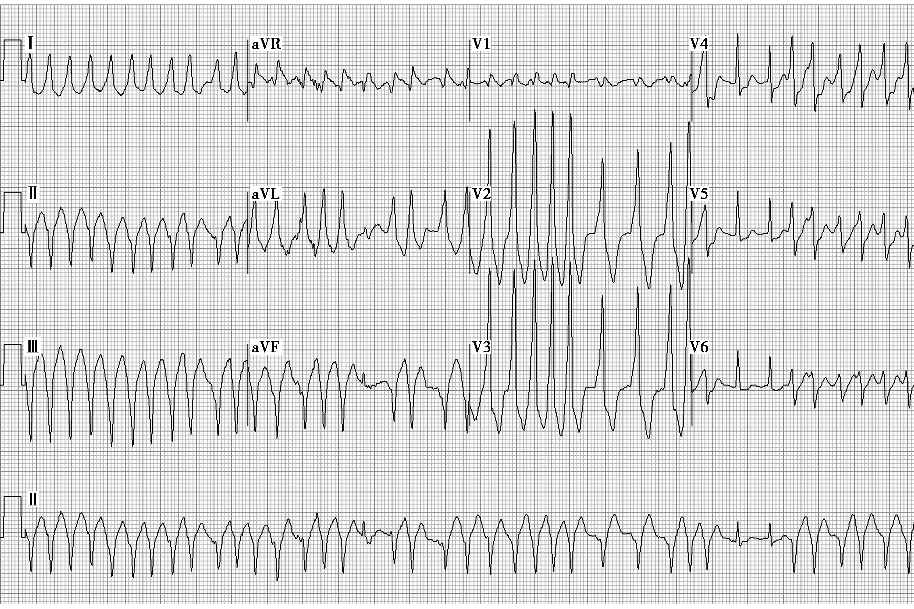
\includegraphics[width=6.29167in,height=4.19792in]{./images/Image00449.jpg}
 \captionsetup{justification=centering}
 \caption{预激综合征合并心房颤动}
 \label{fig102-13}
  \end{figure} 

\paragraph{中间型}

心房激动经AP和AVN-HPS“均等”下传,QRS波群“交替”出现室上形、部分预激形和完全预激形。其心室率的快慢及对血流动力学的影响均介于上述两者之间。同样可因神经体液改变或误用AVN阻滞剂后使其病情恶化。

WPW伴Af的重要意义在于AP前向不应期短时,其极为快速的心室反应可导致室颤(VF)。WPW并发VF主要见于多条AP、反复性心动过速发作频繁及快速性房颤者,尤其以Af时的最短预激性R-R间期≤250ms者危险性最大。Af时心室率决定于AP前传不应期的长短,不应期愈短心室率愈快;快速下传的激动易落在心室易损期内触发VF;使用缩短AP不应期的药物(如洋地黄、维拉帕米)可使Af恶化为VF;说明Af时的快速房性激动落在心室易损期是突然发生VF的重要生理基础。此外,VF的发生还可能与长时间Af发作引起低血压和继发的心肌缺血缺氧而降低致颤阈和在心室易损期发生室早(RonT)等因素有关。既往认为WPW是一种良性疾患,但近年来已证实WPW患者可以猝死,总发生率0~4\%,绝大多数与Af诱发VF有关。因此,凡是WPW合并Af必须严肃对待,以防猝死。WPW合并Af易误诊为VT,应予以鉴别(表\ref{tab102-15})。

\begin{table}[htbp]
\centering
\caption{WPW伴房颤与室速的鉴别要点}
\label{tab102-15}
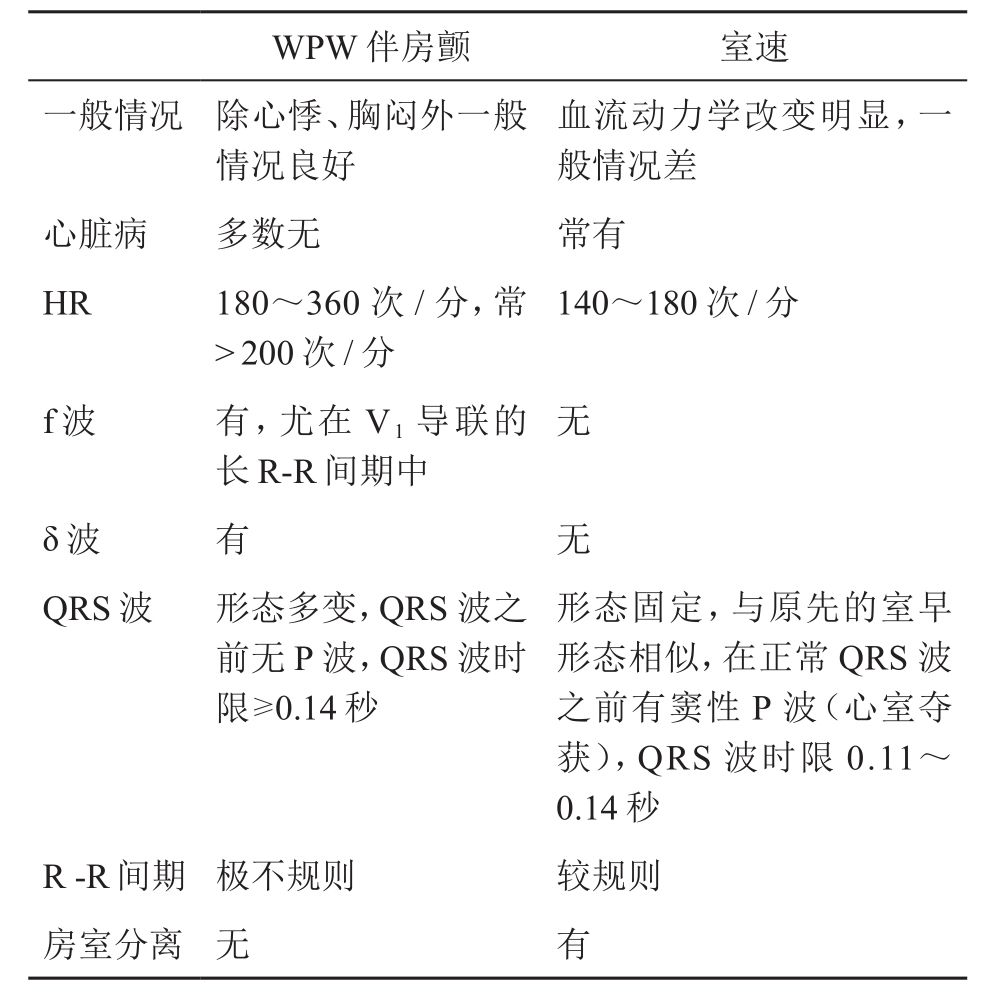
\includegraphics[width=3.27083in,height=3.3125in]{./images/Image00450.jpg}
\end{table}

\subsubsection{持续性房室交界性折返性心动过速(PJRT)}

此类心动过速的特点有:①儿童及年轻人多见,发作时常觉心悸、胸闷,但晕厥少见。②多无明显器质性心脏病,但可因心动过速反复发作而致心功能不全。③心动过速持续时间较长,反复发作,药物疗效不佳。④心电图特征有:a.反复发作的窄QRS波群的心动过速,频率130~220次/分,与窦性心律交替出现。b.常由房性或室性期前收缩、窦性周期(P-R)临界性缩短而诱发。c.发作时P′波在Ⅱ、Ⅲ、aVF、V\textsubscript{2}
~V\textsubscript{6}
导联呈负向,aVR导联正向。d.心动过速开始无P′-R间期延长,R-P′/P′-R >
1或R-P′ > 1/2 R-R(图\ref{fig102-14})。e.发作间期心电图正常。

\begin{figure}[!htbp]
 \centering
 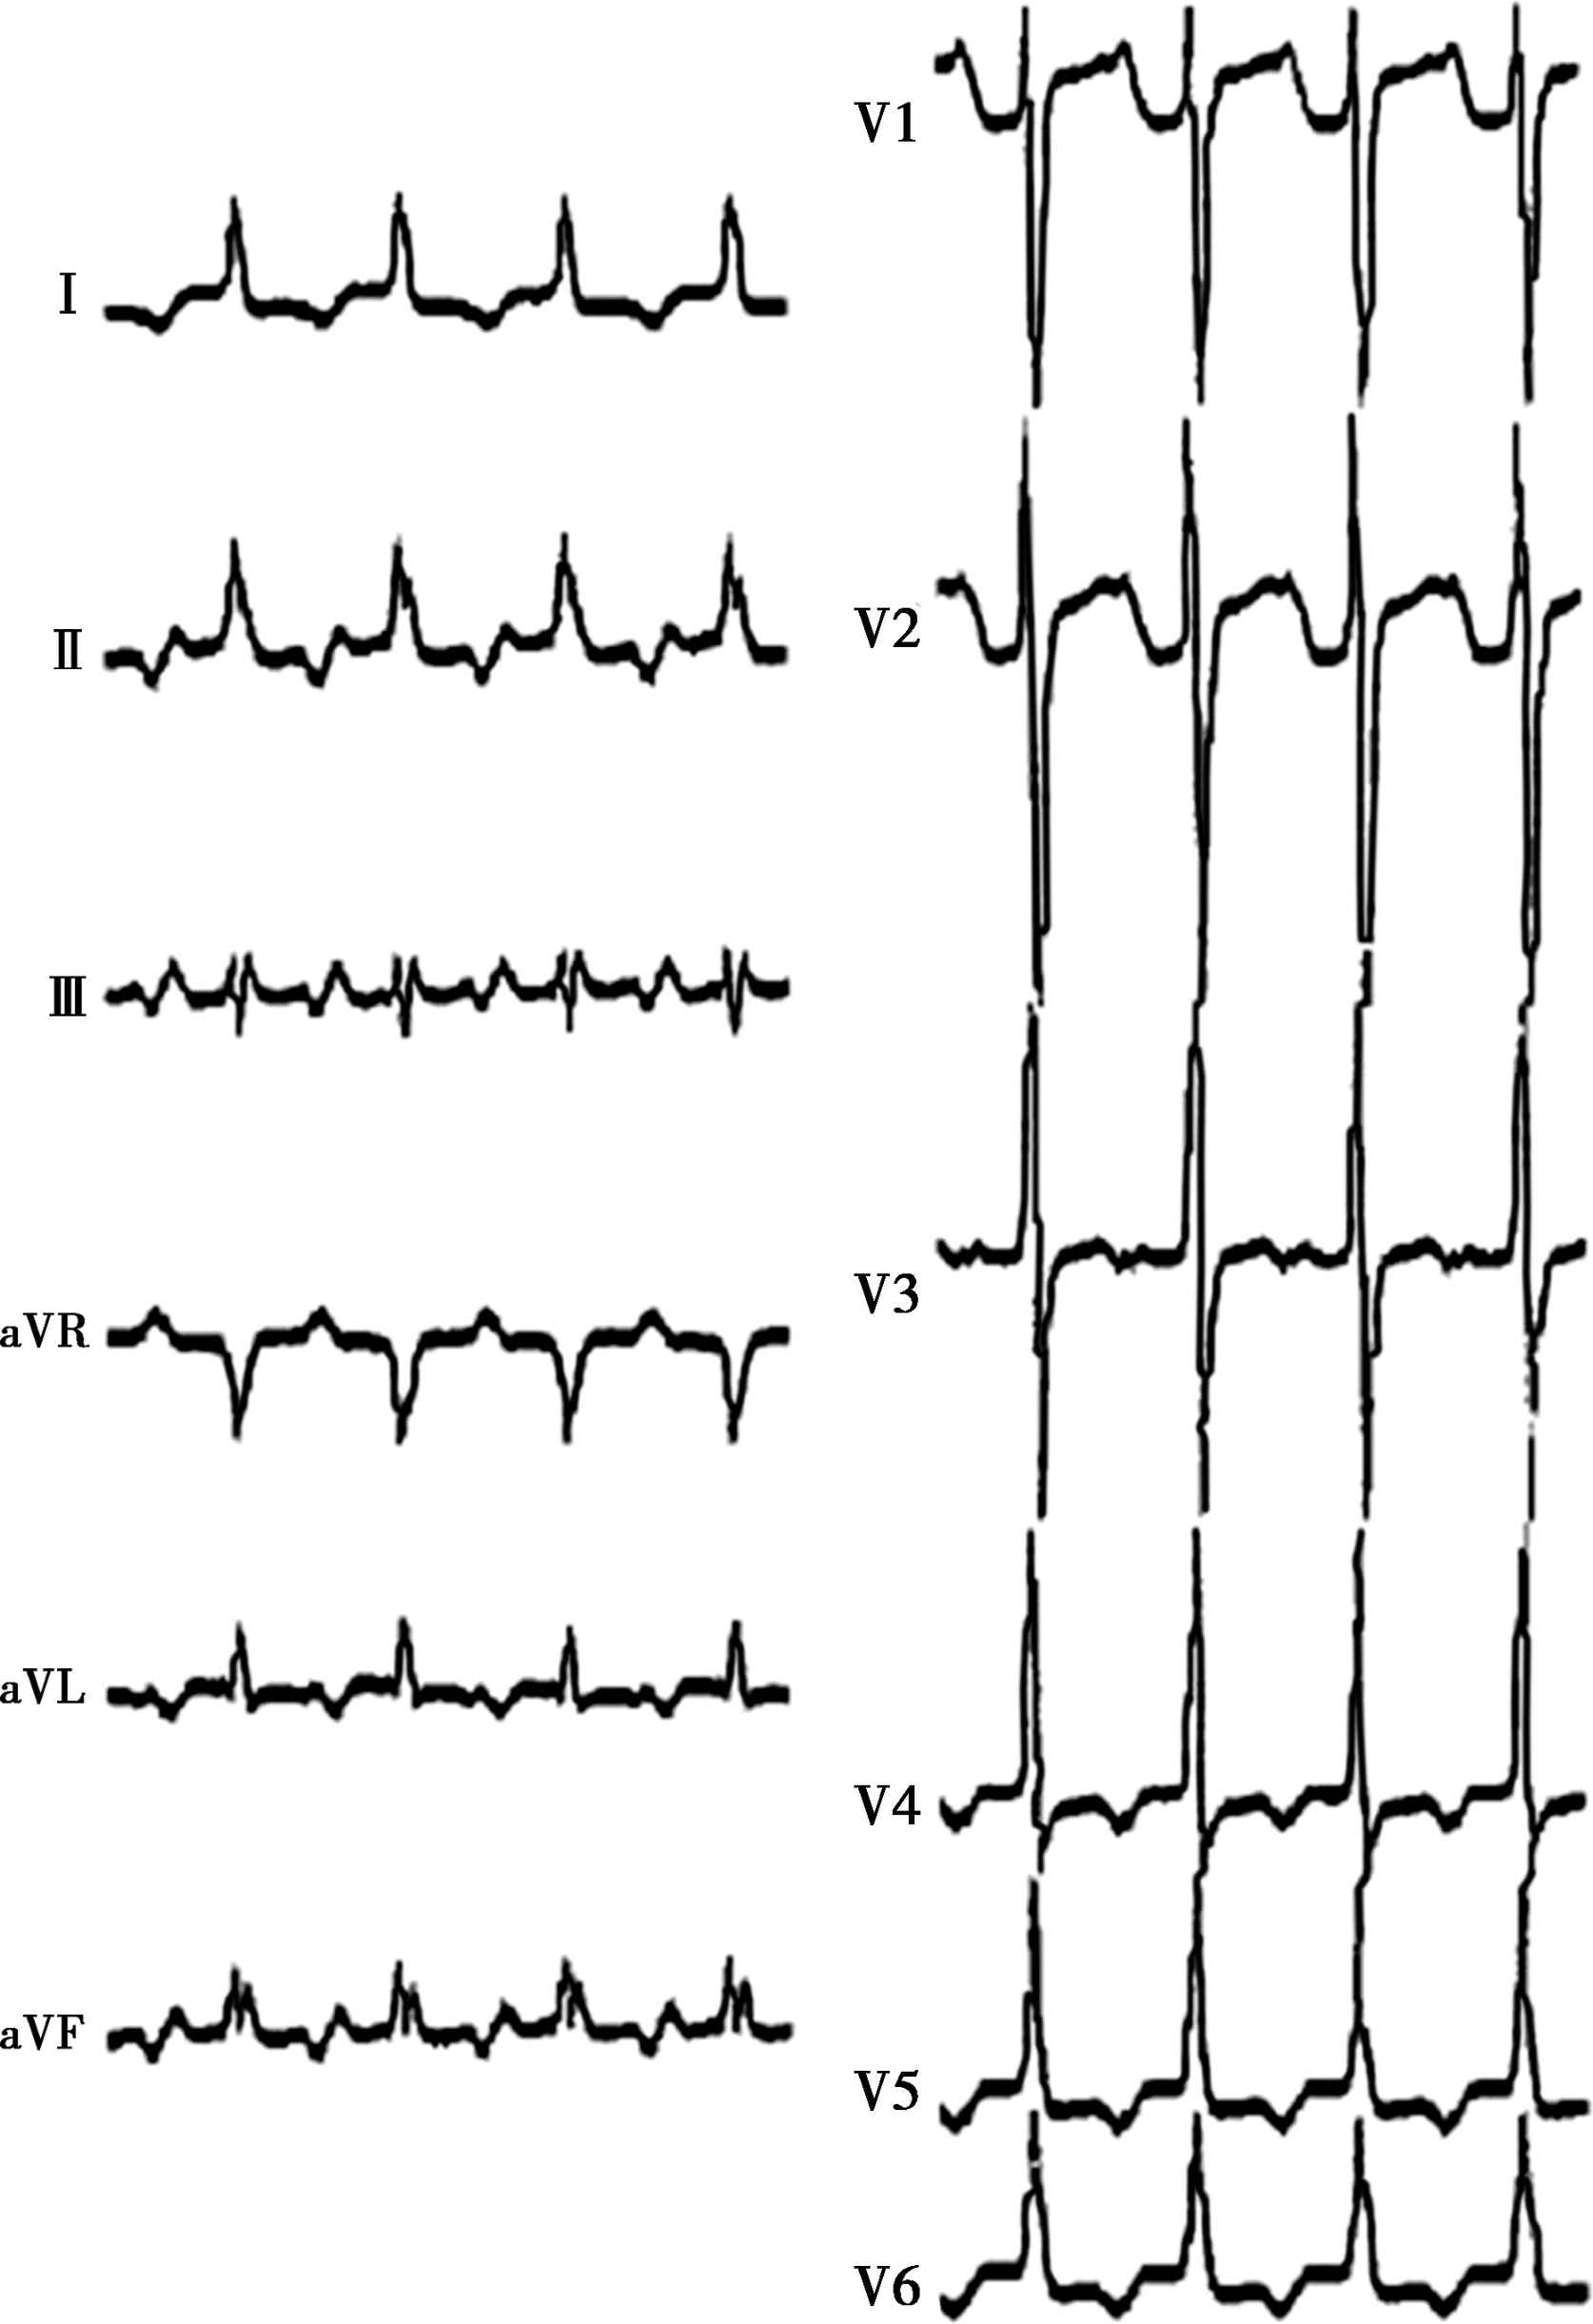
\includegraphics[width=3.10417in,height=4.54167in]{./images/Image00451.jpg}
 \captionsetup{justification=centering}
 \caption{持续性房室交界性折返性心动过速}
 \label{fig102-14}
  \end{figure} 

\subsection{治疗}

单纯的预激综合征无须治疗,但若并发频繁的快速性心律失常则应给予药物治疗、经导管射频消融术(RFCA)或外科手术等。近年来RFCA的临床应用使WPW伴快速心律失常的根治已成为现实,导管射频消融房室旁路的成功率达95\%~98\%。并发心动过速的治疗取决于心动过速发生的机制、心动过速的心室率、心律失常的严重性和患者年龄及心功能状态等。目前常用的治疗措施有药物、电学和外科手术。

\subsubsection{药物治疗原则}

药物依其对AP和AVN的作用,可分为以下三类:

\paragraph{主要作用于 AVN的药物}

普萘洛尔、ATP、洋地黄、维拉帕米等。通过延长AVN不应期,终止折返性心动过速,对治疗OAVRT是安全有效的。但对非束支传导阻滞所致的宽QRS心动过速(即AAVRT)和AP下传为主的Af/AF,普萘洛尔、ATP常无效或可使病情加重而不用;洋地黄缩短AP有效不应期可致病情恶化,应禁用;虽然电生理研究示维拉帕米对AP不应期影响不一,但临床观察证实维拉帕米静注后可使AAVRT恶化为Af/AF或使Af/AF转化为VF,甚至使QRS波群正常的AVRT直接转为VF,故禁用。维拉帕米促发VF的机制是:①缩短AP前向传导有效不应期,加速AP的前向传导;②周围血管扩张和负性肌力作用引起低血压和心排血量减少,导致冠脉灌注不足和心肌缺血。

\begin{table}[htbp]
\centering
\caption{常用药物对房室结与房室旁路不应期的作用及用法}
\label{tab102-16}
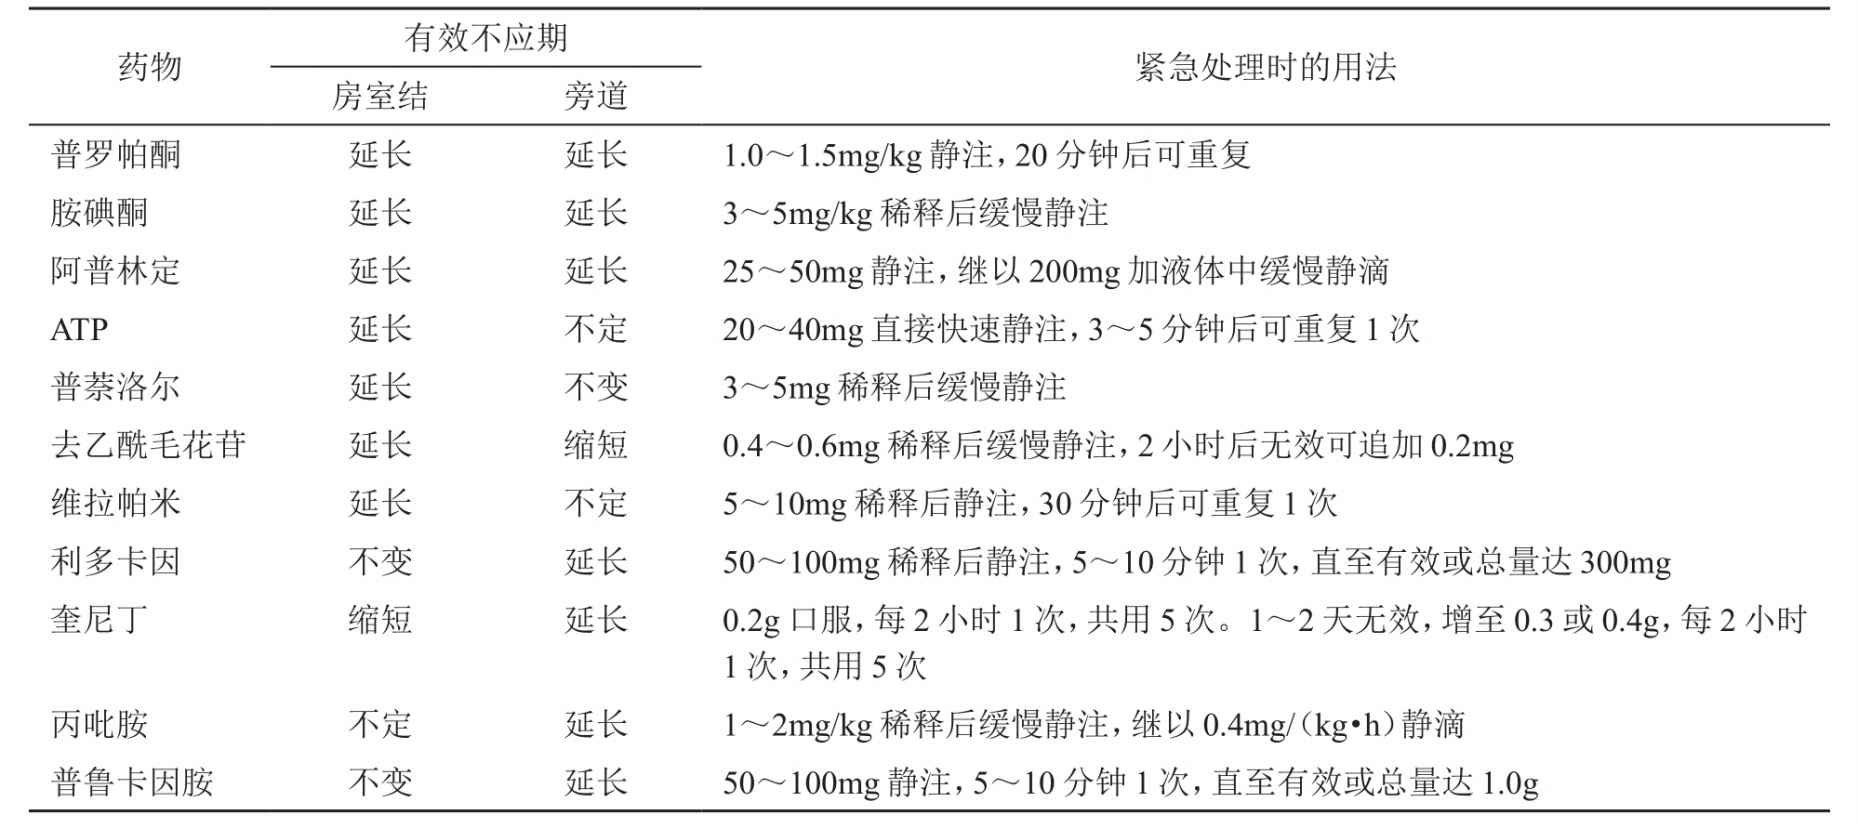
\includegraphics[width=6.65625in,height=2.95833in]{./images/Image00452.jpg}
\end{table}

\paragraph{主要作用于 AP的药物}

常用的有奎尼丁、普鲁卡因胺、丙吡胺、利多卡因、美西律、阿义马林(ajmaline,缓脉灵)等。其共同特征是延长AP有效不应期,主要用于冲动经AP下传的快速性心律失常如AAVRT、Af/AF。奎尼丁尚有缩短AVN有效不应期的作用,可用于伴SSS者。

\paragraph{作用于 AVN和AP的药物}

常用的有胺碘酮和Ⅰc类药物如普罗帕酮、氟卡尼等。其中普罗帕酮抗心律失常谱广、起效快、副作用小,已被列为预激伴快速性心律失常的首选药物。

药物选择依不同类型心动过速而异:①OAVRT:宜选用延长AVN不应期的药物,如胺碘酮、普罗帕酮、维拉帕米、普萘洛尔、ATP等;②AAVRT:宜选用延长AP不应期的药物,如胺碘酮、普罗帕酮、普鲁卡因胺、利多卡因、奎尼丁等;③WPW伴Af/AF:宜选用延长AP和AVN不应期的药物,如胺碘酮、普罗帕酮、普鲁卡因胺等。

常用药物对AVN与AP不应期的作用与用法见表\ref{tab102-16}。

\subsubsection{电治疗}

\paragraph{直流电复律}

是紧急处理WPW伴任何类型的快速性心律失常最有效的措施。若伴有血流动力学明显障碍(如低血压休克、心绞痛、心衰等)应首选直流电复律;对药物疗效不佳或缺乏有效药物时,亦用电复律治疗。一般用100~150J即可。

\paragraph{经食管心房调搏(TEAP)}

是一种无创性的临床电生理诊断和治疗技术,除了可以揭示潜在预激和隐匿预激的旁道传导特性,作为RFCA术前常规筛选及术后检验效果外,也可以用以终止AVRT,以超速刺激最有效。

\paragraph{射频消融术(RFCA)}

RFCA是治疗WPW伴SVT的一种创伤小、痛苦少、操作简便,安全性高和成功率高的新根治方法。据统计,手术成功率可达99\%,手术死亡率在1/1000左右,是目前国内外最受欢迎、广泛推广的一种根治术。并发症少,有室性心律失常、冠状窦破裂、心包堵塞等并发症。

\subsubsection{手术}

外科开胸切割旁路手术,随着RFCA的广泛开展,目前已较少应用。

\hypertarget{text00294.htmlux5cux23CHP10-2-7-4}{}
参 考 文 献

1. Turley A J,Murray S,Thambyrajah J. Pre-excited atrial fibrillation
triggered by intravenous adenosine:a commonly used drug with
potentially life-threatening adverse effects. Emerg Med
J,2008,25(1):46-48.

2. 何秉贤
.预激综合征心电学的诊断问题.中国心脏起搏与心电生理杂志,2009,23(4):363-366.

3.
熊寿贵,余更生.预激综合征的分子遗传学与电生理学研究进展.国际心血管病杂志,2007,34(4):268-270.

4. 汤建民
,黄振文,李鼎,等.预激综合征患者发生阵发性心房颤动机制的探讨.中国心脏起搏与心电生理杂志,2006,20(5):410-412.

\protect\hypertarget{text00295.html}{}{}

\section{宽QRS波心动过速}

宽QRS波心动过速(wide QRS complex
tachycardia,WCT)是指QRS波时限≥0.12秒、频率≥100次/分、规则或不规则的心动过速。是常见的心脏急症。其包括了数种发病机制与治疗原则均不相同的心动过速,易发生误诊、误治,并常导致严重后果。尽管已有许多临床与心电图(ECG)的鉴别标准,但在临床急诊工作中,对WCT的误诊率仍相当高。误诊的常见原因有:①对ECG的鉴别标准不够熟悉或观察ECG不够仔细。②ECG标准本身存在的局限性,即各项心电图标准中的大多数,是以统计学结果为依据,故任何单一的ECG标准均有局限性,即特异性差,敏感性低,因此,运用不当即可导致误诊。③临床医师认识上的偏差,如以血流动力学状况为鉴别标准,认为VT时血流动力学不稳定,而室上速(SVT)时血流动力学稳定。对WCT的正确诊断和鉴别诊断对治疗及预后的判断均十分重要。

\subsection{病因与发病机制}

宽QRS心动过速的病因包括冠心病、心肌病(包括心肌离子通道病)、心肌炎等器质性心脏病,以及特发性室颤、室速等非器质性心脏病,还包括诱发因素如电解质紊乱、药物等。

宽QRS波心动过速的发生机制:①心动过速起源于心室即室速,占WCT的80\%;②室上速(SVT)(包括房性快速性心律失常)伴室内差异传导,约占15\%~20\%;③SVT伴原已存在的束支阻滞,较少见;④SVT经旁路前传,包括预激并房颤及房室折返性心动过速,约占WCT的1\%~5\%;⑤其他:如起搏器介导的心动过速(PMT)、药物或电解质紊乱导致的希-普系统传导减慢等。

\subsection{诊断}

虽然宽QRS波心动过速的最后确诊依赖希氏束电图,但在多数情况下,通过认真收集患者的临床资料,记录心动过速发作时的12导联ECG和食管心电图,仔细比较心动过速发作前后ECG,对多数WCT可以作出较为正确的诊断。

\subsubsection{病史与临床特征}

1.由于80\%左右的
WCT为室速,故遇到WCT患者,应首先考虑室速,没有充分的根据,不应随意诊断为室上速合并室内传导异常。

2.如为无心脏病史而心动过速反复发作的年轻患者
,则多为SVT伴差传,或与预激综合征有关的室上性心律失常。病史中有冠心病心梗史者,发生心动过速时,诊断为VT的阳性预测值为98\%;有器质性心脏病者,阳性预测值为95\%。用药史很重要,抗心律失常药和三环类抗抑郁药可减慢室内传导,在窦性心动过速、快速房颤、房扑时,易产生差异传导,表现为WCT。少数无心脏病证据的VT患者,QRS波时限也可以不增宽。血流动力学状况、年龄和频率,在VT与SVT之间重叠性很明显,故鉴别意义不太大。虽然LVEF在VT组明显低于SVT组,但该项参数对急诊病例的鉴别并无帮助。

3.症状
WCT的症状可以很轻,亦可很重,表现为晕厥或先兆晕厥、心绞痛、休克等。症状的轻重与心率快慢、心脏基础疾病、心功能有关,而与是否为VT或SVT无关。

4.体检
若能发现房室(A-V)分离的体征如颈静脉出现大炮样A波,第一心音强弱不等与收缩压每搏相差10mmHg以上,支持诊断VT。如迷走神经刺激后(如颈动脉窦按压)心动过速终止,则基本上可排除VT。

5.利多卡因
对VT通常有效而对SVT几无作用;维拉帕米对SVT疗效较肯定但对VT通常疗效较差甚至恶化(少数触发机制VT例外)。

\subsubsection{心电图特征}

\paragraph{房室分离}

心动过速时体表ECG有A-V分离或间歇性V-A传导者,强烈提示为VT。大约50\%左右的VT患者有此征象,但其中仅1/2能从体表ECG上识别,其余仅表现为不同程度的V-A传导(1∶1、2∶1或逆向文氏传导)。当体表ECG不能辨别A-V分离时,记录食管ECG或静注腺苷对揭示A-V分离或不同程度V-A传导阻滞有帮助。

\paragraph{心室夺获或室性融合波}

心动过速频率较慢时,通常于心动过速发作开始记录到少数心室夺获搏动或室性融合波,而且夺获搏动的QRS波正常或接近正常(图\ref{fig102-15})。此为提示VT的重要线索,但该现象仅见于5\%~10\%的病例,故其实用价值不很大。

\paragraph{QRS波时限}

以QRS波时限作为一项鉴别标准时,必须与QRS波形态和既往ECG结合考虑。一般说来,SVT伴RBBB图形时,QRS波时限<
0.14秒,而伴LBBB图形时,QRS波时限<
0.16秒;相反,当WCT为RBBB图形时,其QRS波时限>
0.14秒,而LBBB图形者,QRS波时限>
0.16秒,提示为VT的可能性很大。少数起搏点位于束支水平的VT,QRS波时限<
0.14秒,但QRS波形态为RBBB图形伴电轴左或右偏。

\paragraph{QRS波的形态}

\hypertarget{text00295.htmlux5cux23CHP10-2-8-2-2-4-1}{}
(1) QRS电轴:

当窦性心律时不存在室内传导阻滞,发生心动过速时电轴极度左偏(< −90°±
180°),支持VT,此时,不论其QRS波的形态如何。但当QRS波呈LBBB伴电轴右偏者则仅见于VT,差传呈LBBB时其电轴正常或左偏。

\hypertarget{text00295.htmlux5cux23CHP10-2-8-2-2-4-2}{}
(2) 胸导联QRS波形呈同向性:

V\textsubscript{1} ~V\textsubscript{6}
导联QRS主波一致性向下为负向同向性,V\textsubscript{1}
~V\textsubscript{6}
导联QRS主波一致性向上为正向同向性,二者均可认为是VT。正向同向性必须除外A型WPW伴发的逆传型AVRT。

\hypertarget{text00295.htmlux5cux23CHP10-2-8-2-2-4-3}{}
(3) 心前导联V\textsubscript{1} 的QRS波:

呈rS或RS,起始向上波增宽,是支持激动位于心肌组织内缓慢传导的征象,有别于激动经正常传导系统传导QRS波起始部分陡直向上。

\hypertarget{text00295.htmlux5cux23CHP10-2-8-2-2-4-4}{}
(4) RBBB图形:

心动过速呈RBBB图形者,其V\textsubscript{1} 和V\textsubscript{6}
导联QRS波的形态,有助于鉴别心动过速的起源。V\textsubscript{1}
导联QRS波呈单相(R波)或双相波(qR,QR或RS)者,几乎均见于VT。无论是VT还是SVT,在V\textsubscript{1}
导联均可出现三相QRS波,但是典型rSR′图形(即R′ >
r)都见于SVT伴差传,而呈RSr′(即R > r′)多见于VT。V\textsubscript{6}
导联出现典型RBBB图形,即小q,大R及宽S波者,高度支持为SVT伴差传,如初始q波缺乏且R/S
< 1或呈Qr和QR者,则主要见于VT。

\begin{figure}[!htbp]
 \centering
 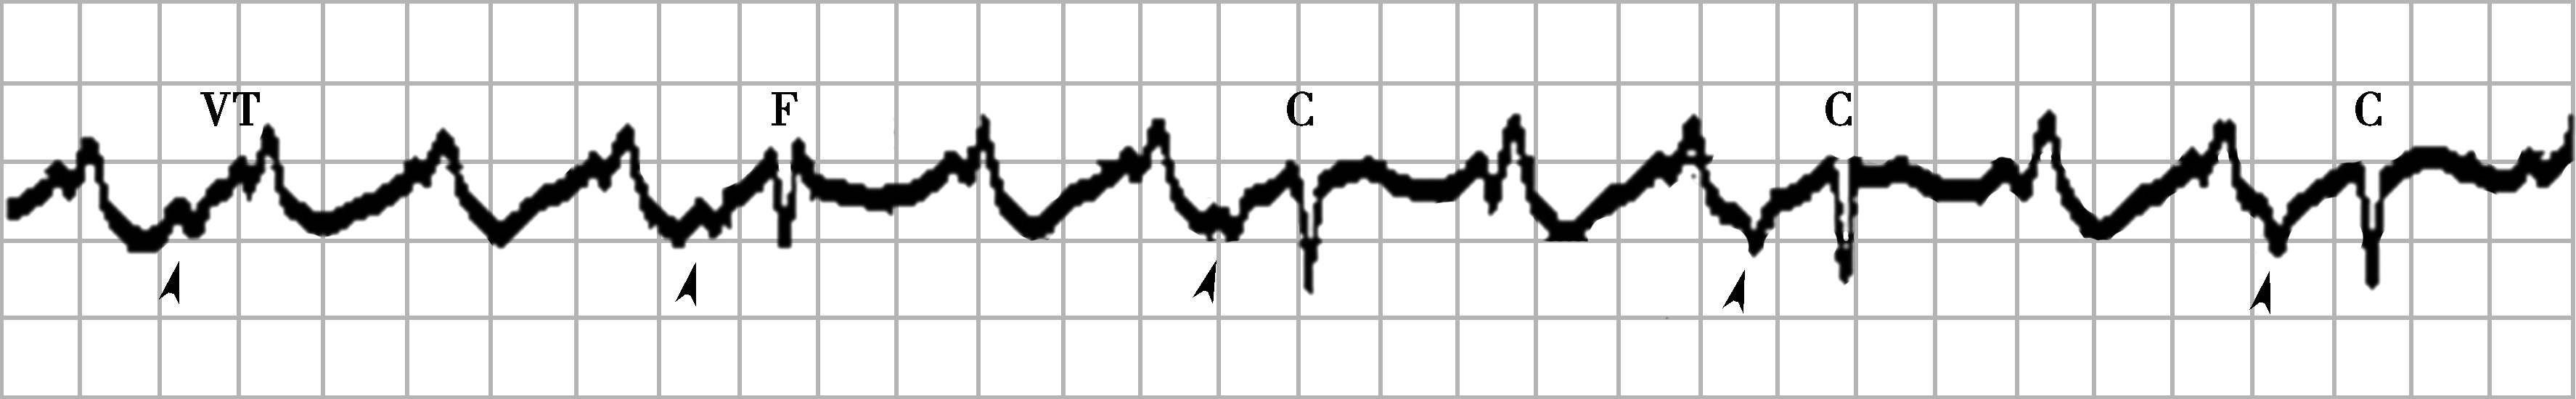
\includegraphics[width=5.90625in,height=0.91667in]{./images/Image00453.jpg}
 \captionsetup{justification=centering}
 \caption{室速(可见室性融合波、心室夺获)}
 \label{fig102-15}
  \end{figure} 

F:融合波;C:心室夺获

\hypertarget{text00295.htmlux5cux23CHP10-2-8-2-2-4-5}{}
(5) LBBB图形:

当V\textsubscript{1} 或V\textsubscript{2} 导联起始r波>
30ms;V\textsubscript{1}
导联S波顿挫或切迹及(或)QRS波起点距S波最低点时限>
70ms者,常见于VT,若同时伴有电轴左偏,则诊断VT的阳性预测值为95\%;V\textsubscript{6}
导联呈qR或QR型则有利于诊断VT,而单相R波有利于诊断SVT。

\hypertarget{text00295.htmlux5cux23CHP10-2-8-2-2-4-6}{}
(6) 窦性心律时ECG存在束支或室内传导阻滞:

发生心动过速后,QRS波形态与窦律的QRS波图形相同者为SVT;反之,与窦律的QRS波图形截然不同者多为VT。

Brugada等根据发作心动过速时宽QRS波的形态,提出了鉴别WCT起源部位的步骤,共分为四步:①所有胸导联均无RS型QRS波,诊断VT的特异性为100\%;②若某一个胸导联出现RS型QRS波者,而最大R至S间期(从R波起点至S波最低点的间距)>
100ms者可确定为VT;③如能确定存在房室分离,VT即可诊断;④如果V\textsubscript{1}
和V\textsubscript{6}
导联的QRS波能满足诊断VT的形态标准(表\ref{tab102-17}\footnote{RBBB:右束支阻滞;LBBB:左束支阻滞;(+):有;(−):无}),即可诊断VT。以此标准判断VT和SVT的符合率分别为98.7\%和96.5\%。Brugada等提出的WCT四步鉴别法如图\ref{fig102-16}所示。临床经验证明Brugada宽QRS波心动过速诊断标准对鉴别不同心室激动时序所致的宽QRS波有高度的敏感性和特异性,但也有缺陷,不能鉴别旁路前传或VT。在后续研究中,该研究组又补充以下3步,合称7步法:①V\textsubscript{4}
~V\textsubscript{6} QRS以负向波为主;②V\textsubscript{2}
~V\textsubscript{6}
中有一个以上的导联呈QR型;③房室分离,P波多于QRS波。以上均阴性诊断为WPW伴旁道前传型SVT。本法对旁路前传型SVT鉴别的灵敏度为75\%,特异度为100\%。

\begin{figure}[!htbp]
 \centering
 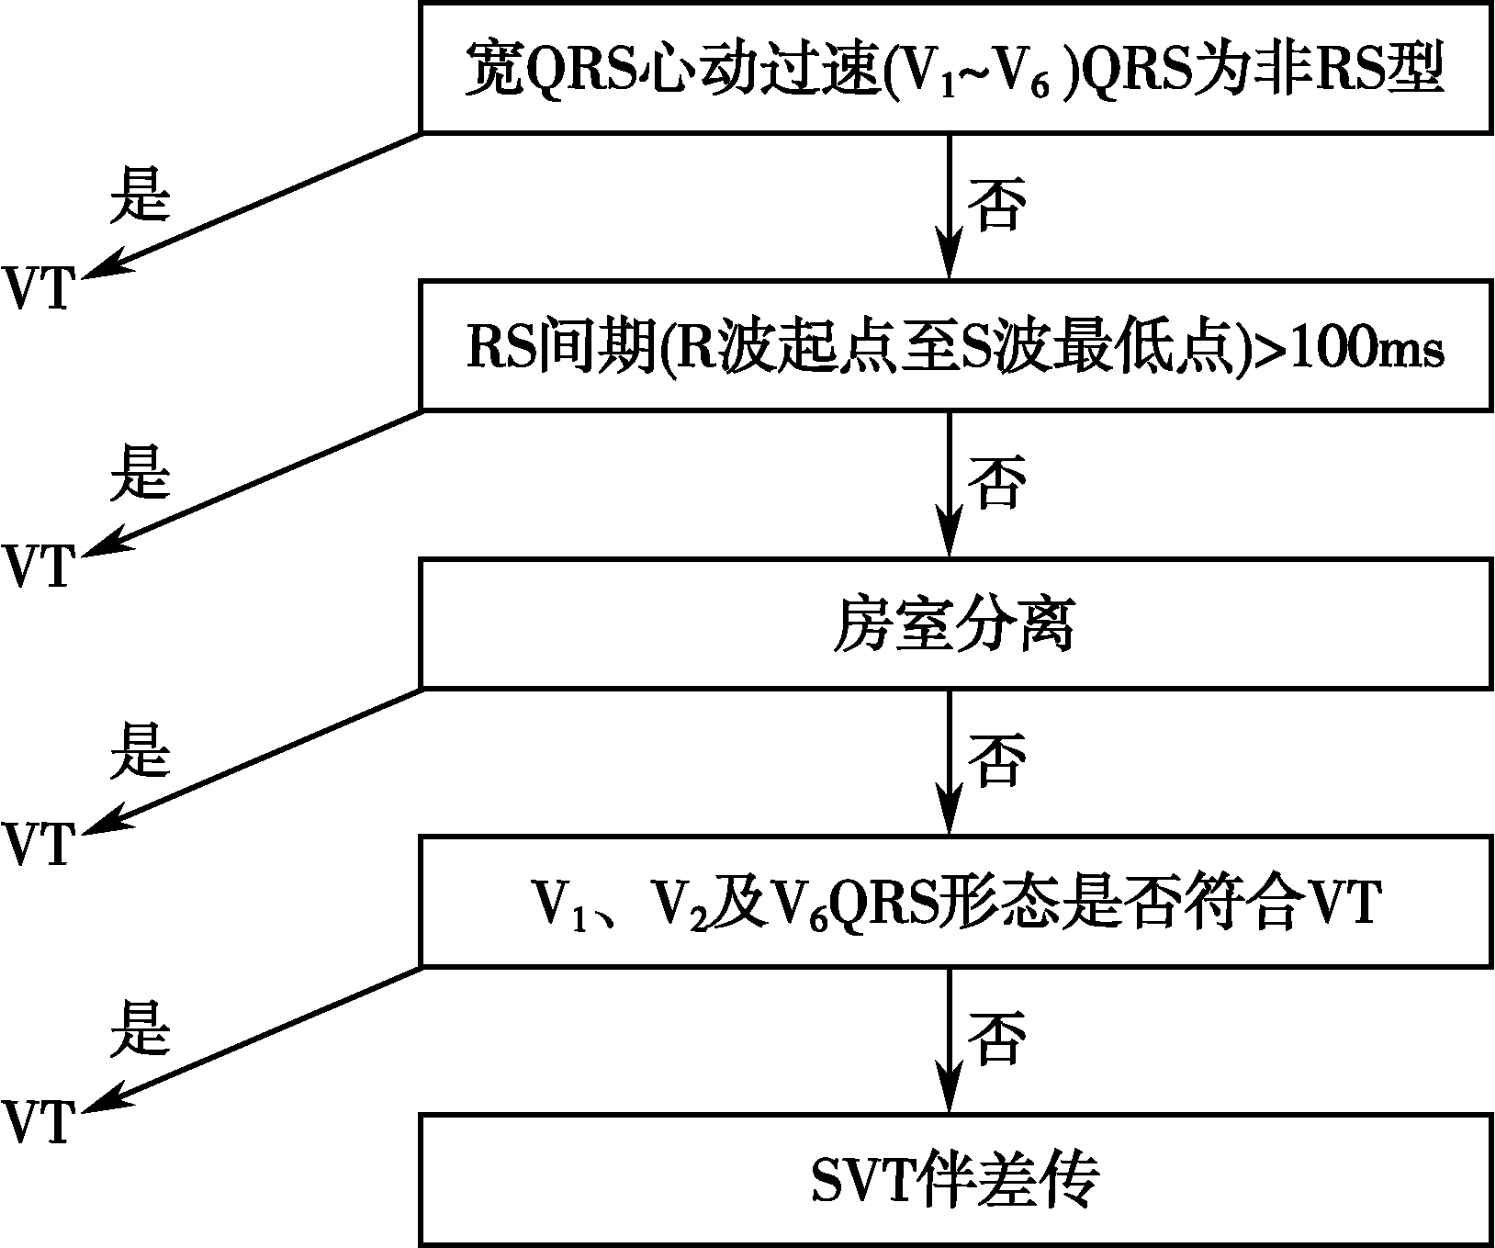
\includegraphics[width=2.70833in,height=2.26042in]{./images/Image00454.jpg}
 \captionsetup{justification=centering}
 \caption{宽QRS波心动过速四步鉴别法}
 \label{fig102-16}
  \end{figure} 

2007年
,Vereckei等提出简化的WCT新四步鉴别诊断流程,但仍复杂,临床医师不易掌握;2008年,Vereckei等又提出了进一步简化的aVR导联四步流程对WCT进行鉴别。具体步骤如下:第一步判断aVR导联QRS波起始是否为R波,如果是则诊断室速,否则为室上速;第二步观察aVR导联QRS波起始r或q波,宽度>
40ms则诊断室速,否则为室上速;第三步以aVR导联负相QRS波为主导的负相起始波降支上出现切迹诊断室速,否则为室上速;第四步测量心室初始激动速度(V\textsubscript{i}
)与终末激动速度(V\textsubscript{t}
)之比,通过测量体表心电图的电压来计算(QRS波起始后移40ms处测得电压绝对值为V\textsubscript{i}
,QRS波终点前移40ms处测得电压绝对值为V\textsubscript{t}
),V\textsubscript{i} /V\textsubscript{t}
≤1诊断为室速,否则为室上速。临床实践表明,以上两种方法对诊断WCT为室速或为室上速的敏感性、特异性相当。

\begin{table}[htbp]
\centering
\caption{宽 QRS波心动过速心电图鉴别标准}
\label{tab102-17}
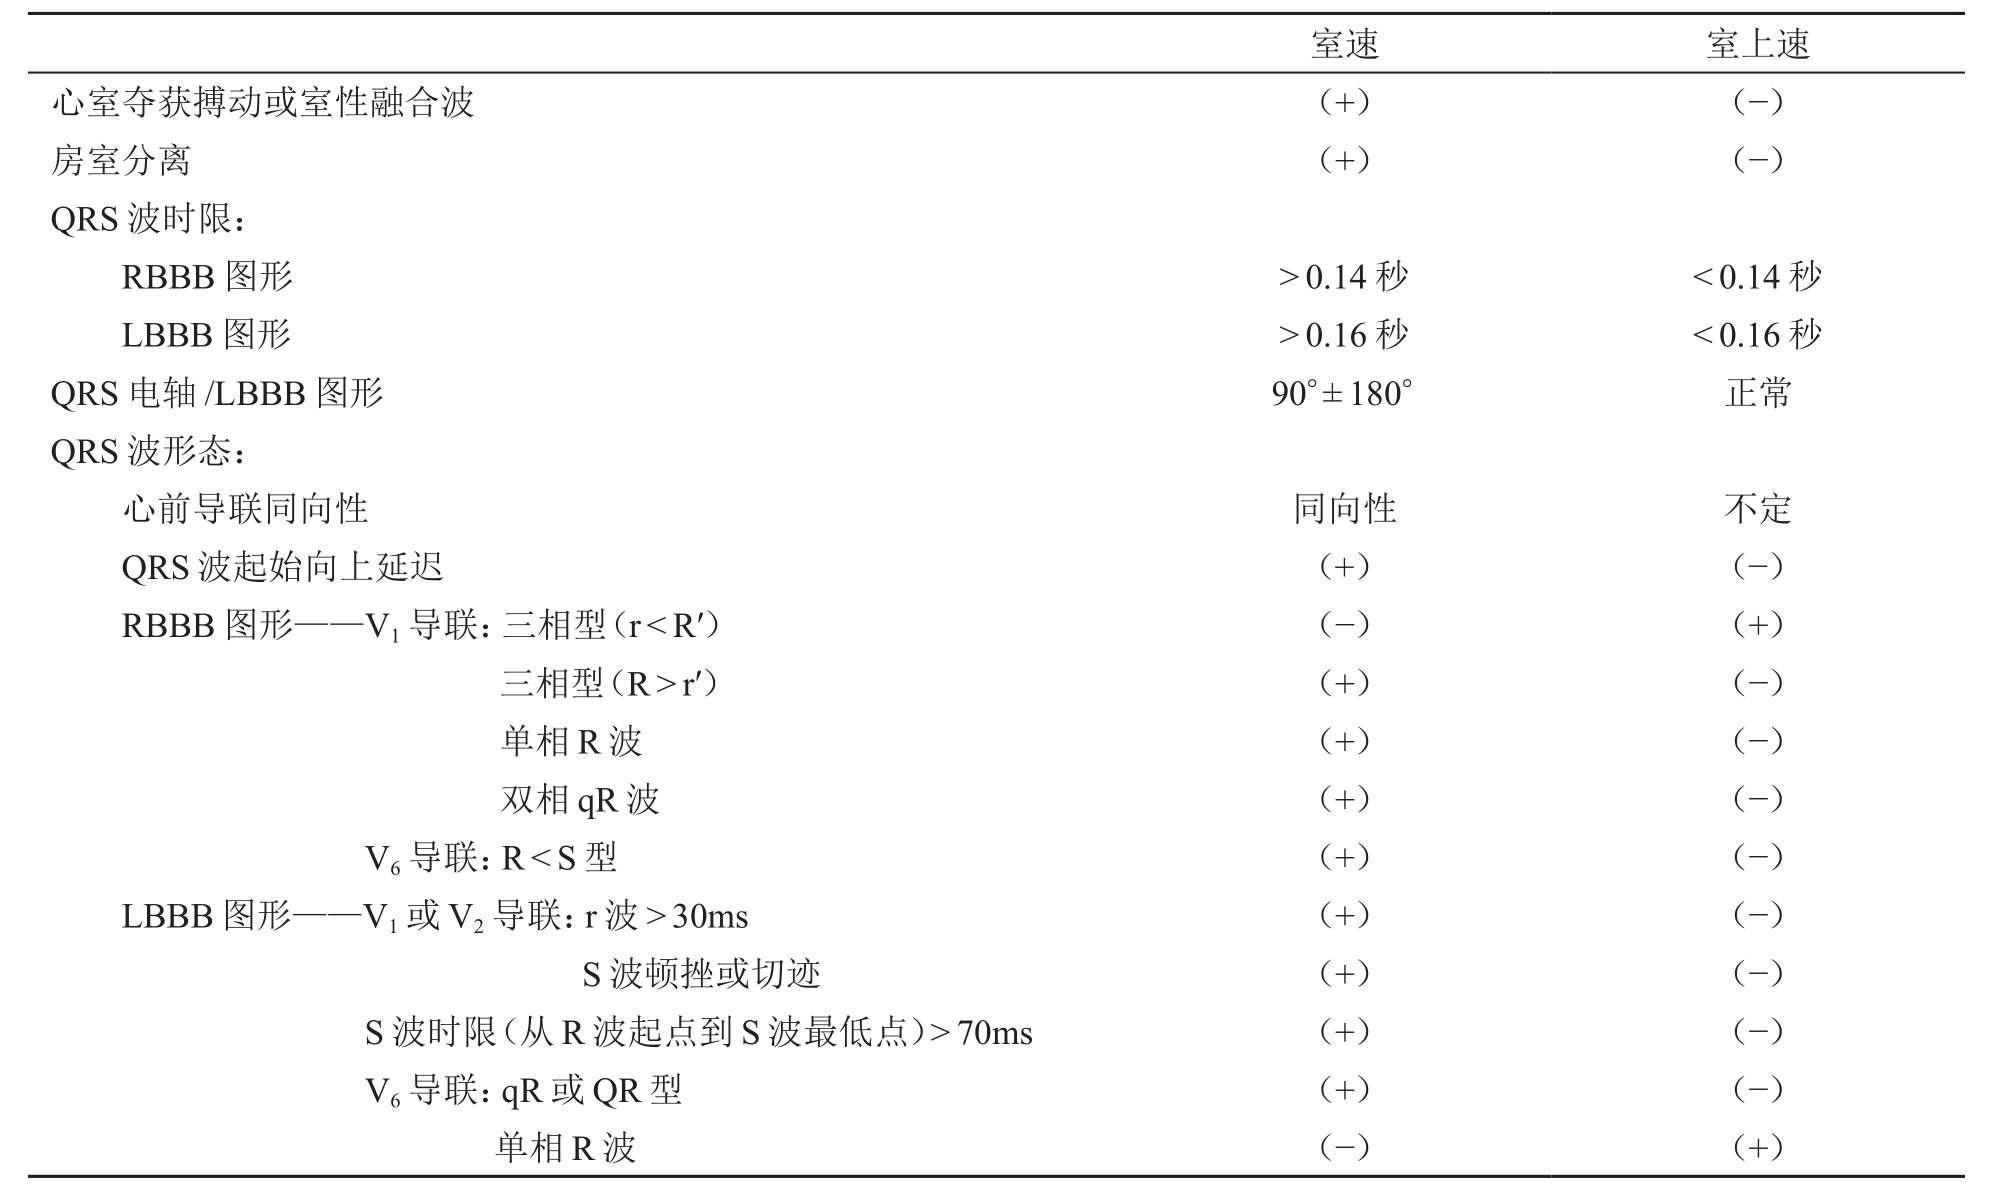
\includegraphics[width=6.65625in,height=3.94792in]{./images/Image00455.jpg}
\end{table}


\paragraph{室上速伴室内差传的独特 ECG改变}

\hypertarget{text00295.htmlux5cux23CHP10-2-8-2-2-5-1}{}
(1) 房颤合并室内差传:

常呈间歇性,很少呈持续性。这是因为室内差传有一定的临界R-R间期长度,房颤时R-R间期长短不一,当R-R间期<临界长度时就会出现室内差传,而当R-R间期>临界长度时室内传导转为正常。房颤合并室内差传也常出现长-短周期心搏,即所谓Ashman现象。房颤合并差传者绝大多数呈RBBB型,V\textsubscript{1}
导联出现rsR′型,起始向量与正常的窦性心搏一致。

\hypertarget{text00295.htmlux5cux23CHP10-2-8-2-2-5-2}{}
(2) 房扑合并室内差传:

可以呈持续性,也可呈交替性,后者较易识别。房扑合并2∶1房室传导时,心室率150
次/分左右,很少发生室内差传。房扑经某些药物(如奎尼丁、普鲁卡因胺)治疗后,房率减慢,房室传导可转变为1∶1,或在某些情况下如交感神经张力过度增高时,房室传导比例也可能为1∶1。当房扑合并1∶1房室传导时可出现持续性室内差传,QRS波宽大畸形,心室率200次/分左右,F波多被掩盖,与VT不易鉴别。按压颈动脉窦常可揭示心律失常的真相。房扑经洋地黄治疗后,可出现4∶1房室传导与2∶1传导交替出现,出现于短心动周期(2∶1房室传导)的心搏可呈室内差传,而出现于长心动周期(4∶1房室传导)的心搏室内传导转为正常,有时可被误诊为室早二联律。

\hypertarget{text00295.htmlux5cux23CHP10-2-8-2-2-5-3}{}
(3) 房速伴室内差传:

房速伴有2∶1房室传导时很少发生室内差传,当房室传导为1∶1时则可能发生室内差传,但比较少见。并有房室传导阻滞的房速经奎尼丁等药物治疗后,房室传导可变为1∶1,且可出现室内差传,此时很容易被误诊为室速。房速的P波多为直立型,但也可为逆传型,当心率过快时,P波常埋没在ST-T内而不易辨认。按压颈动脉窦可引起房室传导阻滞,暴露被隐藏的P波。

\hypertarget{text00295.htmlux5cux23CHP10-2-8-2-2-5-4}{}
(4) AVNRT与AVRT合并室内差传:

AVRT合并室内差传远比AVNRT和房速多见,这可能由于旁道传导速度较快,当激动由旁路逆传、折返前传至心室时,一侧束支可能处于不应期,因而发生室内差传。有学者认为LBBB型室内差传几乎毫无例外地见于AVRT。当旁路与频率性束支传导阻滞同侧时(例如左侧旁路合并LBBB型室内差传,右侧旁路合并RBBB型室内差传),激动必须绕行对侧束、室间隔,才能抵达旁路的心室附着处,折返环路延长,V-A间期与R-R间期延长,心率随之减慢。出现室内差传而伴有心率减慢,为旁路加入心动过速形成(AVRT)的有力佐证。

\paragraph{预激综合征合并房颤}

WPW合并房颤时,心房激动可沿房室交界区或旁路前传至心室,也可同时沿上述的两条途径前传至心室,形成“室性融合波”。当心房激动沿房室交界区前传至心室时,QRS波群形态、时间正常,与一般的房颤无法鉴别;当心房激动沿旁路前传时,QRS波宽大畸形,如并发于A型预激综合征,心前导联均出现正向的宽QRS波,酷似VT。有时在同一份心电图上可见到三种波形:正常QRS波(房室交界区前传)、宽QRS波(旁路前传)与程度不同的“室性融合波”(同时沿旁路与房室交界区前传)。WPW并房颤的ECG改变有其特点,仔细观察不难与VT相鉴别:①R-R间期极不规律,互差常>
0.10秒;②宽QRS波起始部分可见到预激波;③心室率> 180~200 次/分,甚至>
240次/分;④宽QRS波与正常QRS波在同一份心电图内出现时,正常QRS波往往延迟出现(房室结传导速度慢),而不是提早出现(室速的心室夺获多提早出现)。(图\ref{fig102-17})

\begin{figure}[!htbp]
 \centering
 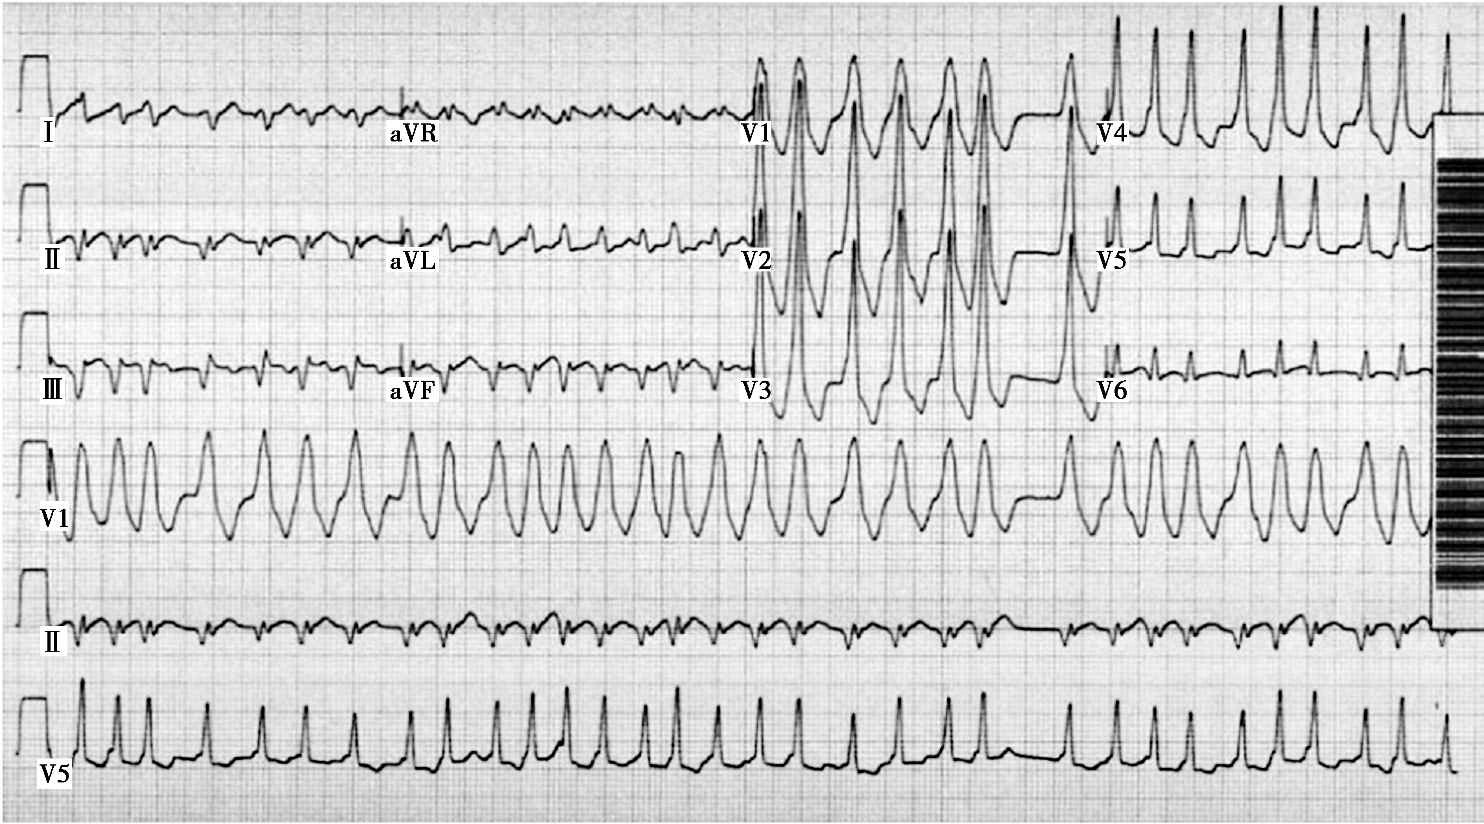
\includegraphics[width=6.29167in,height=3.48958in]{./images/Image00456.jpg}
 \captionsetup{justification=centering}
 \caption{预激伴房颤,除QRS增宽外,QRS形态多变,可与预激伴原已存在的束支传导阻滞鉴别;因R-R间期越短,QRS越窄,系传导加速所致,可排除SVT伴差传}
 \label{fig102-17}
  \end{figure} 

\subsubsection{电生理检查}

临床心脏电生理检查在鉴别WCT的起源部位时是最可靠的方法。①希氏束电图(HBE)表现为A、H和V波呈固定关系,H-V间期略长于窦律时H-V间期,为室上速;若心动过速发作时A-H有固定关系,而A-H与V波间无固定关系,且A-H频率慢于V波频率,为VT。②若H-V间期短于窦律时的H-V间期或V波前无H波,则心动过速的QRS波除完全或部分起源于心室外,还可能由于Mahaim纤维前向传导引起的H-V间期缩短或H波与V波的重合。在Kent束参与前向传导的SVT,也可以看不到H波或在V波前无固定的H波,但此时逆传的V-A存在固定关系。③V波前有H波且H-V波间期与窦律时相等,为心室夺获;H-V间期<窦律时的H-V间期,为心室融合波。④WCT心房起搏夺获心室后变窄,则为VT;快速起搏心房时功能性束支阻滞,如与发作时波形相同,则为SVT合并室内差传。⑤食管内导联与心房内导联心电图可明确地显示心房波形,心房活动的频率、房室传导与室房传导的关系、R-P间期的长度等,对鉴别VT与室上速、房扑、AVRT与AVNRT等均有很大价值。

\subsection{治疗原则}

对WCT患者,应仔细分析心电图改变,结合病史、体检与颈动脉窦按压,作出明确诊断(明确起源部位),再给予适宜处理。对于一时难于鉴别起源部位的WCT,可采用以下“中性”治疗方案:

\paragraph{血流动力学明显障碍者}

若WCT伴有明显的血流动力学障碍(如心室率极快、心衰加重、低血压、休克、心绞痛),甚至阿-斯综合征时,若能排除洋地黄中毒,应立即首选直流电复律,首次电击能量不应超过200J,必要时可重复进行。对长时间用药不能纠正的WCT,不论是否确定其起源部位,也应行同步直流电复律。

\paragraph{血流动力学状态较稳定者}

对难以鉴别的且血流动力学稳定的WCT,可首先按VT处理,或者选择对室上性及室性心律失常均有效,同时又不缩短房室旁路前传时间及有效不应期的药物如胺碘酮、普罗帕酮(心律平)、普鲁卡因胺及阿普林定(安搏律定)等,其对室上速、室速和WPW合并房颤均有效,以静脉制剂为宜。用药过程中应监测心电图与血压的改变,并准备好除颤起搏器,以防药物诱发VF或心脏停搏。必须指出的是,对诊断不明的WCT,应禁用洋地黄、维拉帕米或腺苷类。这三种药物对VT均不适宜,尤其是静注维拉帕米可使VT患者血压明显降低,甚至诱发VF。对于确定或高度怀疑对维拉帕米有“特效”的室速如特发性室速(无器质性心脏病,心电图示QRS时限≤0.12秒,多呈RBBB
+电轴左偏)、QT间期正常和期前收缩联律间期极短的多形性室速等,可选用维拉帕米。洋地黄与维拉帕米使旁路不应期缩短,致使旁路前传的心房颤动与旁路前传型心动过速心室率异常增速,如落入心室易损期可诱发VF。腺苷类药物对房速也不适宜,可引起一过性房室传导阻滞。

血流动力学稳定的宽QRS心动过速的急诊处理程序见图\ref{fig102-18}。

\begin{figure}[!htbp]
 \centering
 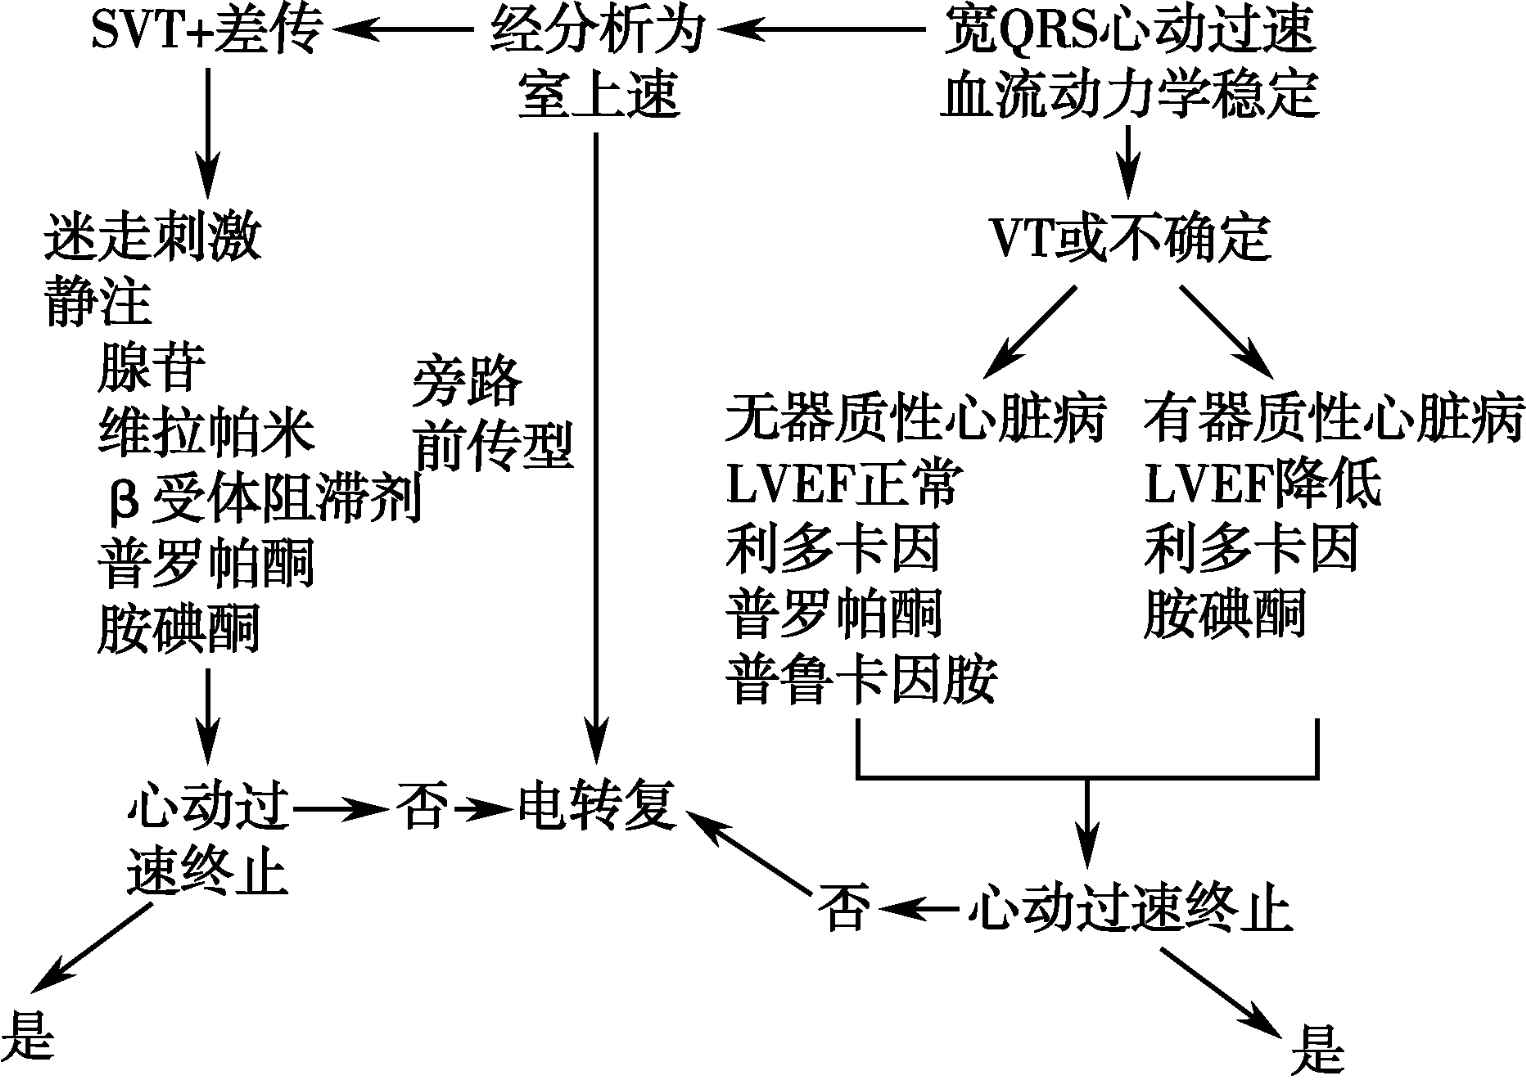
\includegraphics[width=3.10417in,height=2.20833in]{./images/Image00457.jpg}
 \captionsetup{justification=centering}
 \caption{血流动力学稳定的宽 QRS心动过速的急诊处理程序}
 \label{fig102-18}
  \end{figure} 

\hypertarget{text00295.htmlux5cux23CHP10-2-8-4}{}
参 考 文 献

1. Alzand BS,Crijns HJ. Diagnostic criteria of broad QRS complex
tachycardia:decades of evolution. Europace,2011,13(4):465-472

2. Vereckei A,Duray G,Szénási G,et al. New algorithm using only lead
aVR for differential diagnosis of wide QRS complex tachycardia. Heart
Rhythm,2008,5(1):89-98

3. Vereckei A,Duray G,Szénási G,et al. Application of a new algorithm
in the differential diagnosis of wide QRS complex tachycardia. Eur Heart
J,2007,28(5):589-600

4. Delacretaz E. Supraventricular tachycardia. N Engl J
Med,2006,354(10):1039-1051

\protect\hypertarget{text00296.html}{}{}

\section{心室扑动和心室颤动}

心室扑动(室扑,ventricular flutter)和心室颤动(室颤,ventricular
fibrillation,VF)分别为心室肌快而微弱的无效收缩或不协调的快速乱颤,二者血流动力学影响均等于心室停搏。室扑常为室颤先兆,很快即转为VF。而VF则是导致心脏性猝死(sudden
cardiac
death,SCD)的常见心律失常,也是临终前循环衰竭的心律改变。原发性VF为无循环衰竭基础上的VF,常为一过性和反复发作,以药物及电复律可逆转。在各种严重心脏病的终末期发生的室扑和VF,为继发性室扑和VF,预后极差。

\subsection{病因与发病机制}

\subsubsection{病因}

各种器质性心脏病及许多心外因素均可致室扑或室颤,以冠心病、原发性心肌病、瓣膜性心脏病、高血压性心脏病为最常见。原发性VF则好发于急性心梗、心梗溶栓再灌注后、原发性心肌病、病窦综合征、心肌炎、触电、低温、麻醉、低血钾、高血钾、酸碱平衡失调、嗜铬细胞瘤和拟肾上腺素药物过量、奎尼丁、普鲁卡因胺、锑剂和洋地黄等药物中毒、QT间期延长综合征、Brugada综合征、预激综合征合并房颤时旁道不应期<
270ms、二尖瓣脱垂综合征等。

\subsubsection{发病机制}

VF的发生机制可分为触发机制和维持机制两方面。

\paragraph{触发机制}

VF可以被发生于心脏易损期的期前收缩诱发,即“R on
T”现象。然而,VF也可在没有“R on
T”的情况下发生,故有理论认为当一个行进的波阵面碰到解剖障碍时可碎裂产生多个子波,后者可以单独存在并作为高频率的兴奋起源点触发VF。目前多数学者认为心室肌结构的不均一是形成自律性增高和折返的基质,而多个研究都提示起源于普肯耶系统的触发活动在VF发生起始阶段的重要作用。

\hypertarget{text00296.htmlux5cux23CHP10-2-9-1-2-1-1}{}
(1) 普肯耶细胞的早期后除极:

普肯耶细胞的早期后除极(early
afterdepolarizations,EAD)引起的触发活动与室性心律失常有关,EAD在动作电位2相和3相振荡的基础上发生。细胞电生理研究表明普肯耶细胞和心室肌细胞电生理性质存在显著的差异,表现在普肯耶细胞的膜阻抗远比心室肌细胞高,动作电位时程(APD)也比心室肌细胞长。普肯耶细胞固有的膜阻抗较高的性质使得很小的内向净电流的增加就可以促进EAD的形成,所以EAD的形成和传导在普肯耶纤维中显得比较容易。正常情况下,在普肯耶-心室肌交界处(PMJ)由于二者膜阻抗的差异,较小的偶联电流引起普肯耶细胞膜电位的变化大于对心室肌膜电位的影响,所以在相互作用中心室肌膜电位“控制”了普肯耶膜电位。尽管固有的静息电位、平台期电位和APD与心室肌细胞不同,细胞间的偶联作用使普肯耶细胞的这些性质与偶联的心室肌细胞相接近,所以偶联的普肯耶细胞APD会明显短于远离PMJ的普肯耶细胞。APD的缩短不利于EAD的发生。病理条件下,普肯耶细胞本身的自律性增强,或者失去交界区电偶联的约束,或者产生损伤电流通过PMJ加剧普肯耶细胞膜电位的振荡,都可以导致普肯耶细胞EAD的产生而触发室性心律失常。梗死条件下大量心室肌细胞的坏死使普肯耶纤维和心室肌的膜阻抗比例失调而失去对偶联普肯耶细胞EAD的抑制作用,加之梗死区存活的普肯耶细胞最大除极速率下降和APD明显延长,导致交界区动作电位的3相EAD,除极到达阈值以后触发心室激动。

\hypertarget{text00296.htmlux5cux23CHP10-2-9-1-2-1-2}{}
(2) PMJ的折返激动:

PMJ的折返激动也可能是恶性室性心律失常和VF的触发因素,普肯耶-心室肌传导和心室肌-普肯耶传导的不对称是折返产生的基质。不论在左右心室,束支下传的激动都只能够通过乳头肌基底部的PMJ传递到心室肌,并且高的阻抗比值导致传导延迟,而从心室肌逆传的激动则可以在PMJ以外的广泛区域发生,传导速度也快于前者。PMJ的传导延迟可以被奎尼丁、高钙以及超速起搏加重,折返活性也会增加而诱发心律失常。

\paragraph{维持机制}

有关VF的维持机制存在较大的争议。争议的焦点在于如何解释VF发生过程中的持续的波裂(wave
break)现象:新形成的波裂究竟是导致了VF的维持的原因(多重子波学说),还是仅仅作为源自高速运转的局灶起源(a
rapid firing focal
source)的激动不能保持1∶1外传的外在表现(局灶起源学说)。

\hypertarget{text00296.htmlux5cux23CHP10-2-9-1-2-2-1}{}
(1) 多重子波学说:

该学说认为,通过波裂连续不断产生的多重子波随机折返导致VF的发生。波裂的发生是由于不应期分布的不均一和解剖学上的异质性使得兴奋波呈现不均一传导的结果。不应期分布的不均一来自于动作电位时程在心室不同部位和心室壁不同层面的离散,这种原本就存在的异质性可以被各种疾病所放大。心外膜走行的冠状动脉,乳头肌,跨壁纤维走向的改变部位以及心肌病中的纤维化部位等,都可以成为兴奋波破裂的位点。近来发现电学恢复(electrical
restitution)中的动态因素即APD和激动传导速度(conduction
velocity,CV)的恢复特性也在波裂形成中发挥重要作用。该学说强调动态因素和固有异质性之间的协同作用是波裂发生和VF维持的基本原因。

\hypertarget{text00296.htmlux5cux23CHP10-2-9-1-2-2-2}{}
(2) 局灶起源学说:

该学说认为单一的快速兴奋灶起源(折返或自律性增高)是VF的基本驱动力。Jalife等提出VF中的激动频率最高的区域(25~30Hz)是由于一个高速运转的折返自卷波即“旋转子”持续活动所致,颤动的传出阻滞发生于旋转子外围的组织,两者一起构成心室肌表面不连续的主导频率控制区。VF中出现的多重子波是起源于这一局灶位点的激动,由于周围组织的“传出阻滞”(fibrillatory
conduction
block)而不能保证1∶1外传的外在表现。该理论的临床意义在于可以对局灶起源部位施行消融来治疗这种恶性室性心律失常。

\paragraph{室颤的电生理分期与分型}

Wiggers等提出VF的发生过程可以分为4个独立的阶段:第一阶段(快速收缩期,tachy
systolic)持续时间为数秒,特点是单个螺旋波或“8”字折返,落入这个时期的期前收缩可以终止折返而预防VF的发生;第二阶段(痉挛性失调期,convulsive
incoordination)持续15~40秒左右,特点为多发子波和折返激动共存;第三阶段(震颤性失调期,tremulous
incoordination)持续2~3分钟,VF的激动频率开始下降,内膜和外膜心肌之间开始出现兴奋性的梯度分布,可能是因为内膜心室肌和普肯耶纤维比其他部位心肌更能够耐受缺血;第四阶段(终末期)是弛缓的颤动,心脏的机械收缩消失。

Wiggers和Chen同时还将VF分为两型:快速室颤(Ⅰ型VF)的主导频率较高,标测特点为游走的子波和持续时间很短的折返波,其前提是复极动力学和细胞兴奋性正常(APD恢复曲线陡峭,CV恢复曲线平坦),符合多重子波学说的特点;缓慢室颤(Ⅱ型VF)的主导频率较低,很少表现为不同波的碰撞,标测多表现为从固定区域起源的单一波阵面在心外膜的播散,其前提是复极异常和兴奋性下降(APD恢复曲线平坦,CV恢复曲线陡峭),符合局灶起源学说的特点。Ⅰ型VF和Ⅱ型VF实际上代表了VF的不同阶段,Ⅰ型VF为起始阶段(Ⅰ,Ⅱ期)的VF,通常在APD恢复曲线陡峭而细胞兴奋性正常的情况下发生;随心肌缺血程度的加重,先是复极功能异常,接着心肌细胞兴奋性下降,此时的VF为Ⅱ型VF(Ⅲ,Ⅳ期)。两型VF中间的过渡阶段,表现为复极异常但兴奋性尚属正常,可以出现暂时的VF发作。

\subsection{诊断}

\subsubsection{临床表现特点}

典型表现为阿-斯(Adams-Stokes)综合征:患者突然抽搐,神志不清,面色苍白,随几次断续的叹息状呼吸之后,呼吸逐渐停止;此时查心音、血压、脉搏均消失,瞳孔散大。如发作为间歇性,则在间歇期可听诊到不规则心搏(常为多源性室性期前收缩)或快速心搏(室速),心音较弱。部分患者阿斯综合征表现不明显即已猝然死亡。

\subsubsection{心电图特点}

\paragraph{心室扑动}

室扑在心电图上表现为连续出现的畸形QRS波群,呈正弦波曲线,QRS波群、ST段和T波混在一起无从辨识,也无法明确为负向波或为正向波。频率150~300次/分(通常在200次/分以上)。有时难与VT鉴别。室扑常为暂时性,大多数转为VF,是VF的前奏;但也可转为室速,极少数恢复窦性心律。室扑与室速的区别在于后者QRS与T波能分开,波间有等电位线,且QRS时限不如室扑时宽,参见表\ref{tab102-11};其与VF的区别在于后者波形及节律完全不规则,且电压较小。

\paragraph{心室颤动}

P波及QRS、T波均消失,代之以形状不同、大小各异、极其不匀齐的波群,频率极快,约250~500次/分,在开始时振幅尚较大,以后逐渐变小,终于消失。

室扑和VF的心电图表现见图\ref{fig102-19}。

\subsubsection{临床分型}

根据临床循环功能、有无器质性心脏病、心电图颤动波的振幅及频率等,可以将VF进行进一步的分型,有助于治疗和预后的判断。

\paragraph{根据室颤波振幅分型}

①粗颤型:VF波振幅≥0.5mV,多见于心肌收缩功能较好的患者,心肌蠕动幅度相对粗大有力,张力较好,对电击除颤效果好,预后相对好,应立即电除颤。②细颤型:VF波振幅<
0.5mV,多见于心肌收缩功能较差的情况。此时心肌的蠕动纤细无力,张力差,对电击除颤疗效较差,预后恶劣。

\paragraph{根据室颤波频率分型}

①快速型:VF波频率> 100
次/分,预后相对好,除颤成功率高。②缓慢型:VF波频率<
100次/分,预后差,多为濒死表现,常继以全心停搏。

\paragraph{根据室颤前心功能分型}

①原发性室颤:又称非循环衰竭性VF。VF前无低血压、心力衰竭或呼吸衰竭,循环功能相对良好,VF的发生与心肌梗死等急性病变有关。除颤成功率约为80\%,此型预后相对较好。②继发性室颤:又称循环衰竭性VF。VF前常有低血压、心力衰竭或呼吸衰竭,常同时存在药物、电解质紊乱等综合因素,电除颤成功率低(≤20\%),预后恶劣。③特发性室颤:VF发生前后均未发现器质性心脏病,VF常突然发生,多数来不及复苏而猝死,部分自然终止而幸存。VF幸存者常有复发倾向,属于单纯的心电疾病。④无力型室颤:又称临终前VF。垂危患者临终前心电图约有50\%可出现VF,其特点为VF波频率慢,振幅低,属于濒死心电图的一种。

\subsection{治疗}

\subsubsection{紧急抢救}

若电除颤器就在手边,立即以150~200J(双向波除颤器)或300~360J(单向波除颤器)进行电除颤。在实施一次电除颤后,不要急于检查患者脉搏,而应马上继续CPR,待完成按压/吹气五个30∶2的周期(大约2分钟)以后,再检查患者的循环征象,评估除颤效果,标志为自主循环和窦性心律是否恢复。如VF波甚细,可在除颤前静注肾上腺素1mg和(或)血管加压素40U,使颤动波变粗,有利于除颤。除颤未成功、或除颤后VF又反复发作者可应用胺碘酮300mg静注和(或)利多卡因1.5mg/kg静注,并重复电除颤。若电除颤器不在手边,应立即叩击心前区或(和)行胸外心脏按压,人工呼吸;同时可试用上述药物除颤或准备电除颤。详见本书第101章“心脏骤停与心肺复苏”部分。

\subsubsection{病因处理}

由严重缺钾引起的VF反复发作,应静滴较大量氯化钾,一般用2~3g氯化钾溶于5\%葡萄糖液500ml内,最初24小时内常需给氯化钾10g左右;治疗持续到心电图上缺钾表现消失为止。由锑剂中毒引起反复VF者,可反复用阿托品1~2mg静注或肌注;同时也应补钾。由奎尼丁或普鲁卡因胺毒性反应引起的VF则不宜用利多卡因,需用阿托品或异丙肾上腺素治疗。如VF发作的间歇中基本心率较慢,并频发室性期前收缩,可试用0.2mg\%异丙肾上腺素静滴。

\subsubsection{心脏复苏后处理}

包括维持呼吸、循环稳定、防治脑水肿及脏器功能不全等,参见有关章节。

\subsubsection{其他治疗措施}

包括埋藏式自动除颤器(ICD)、射频消融等,有指征、有条件时可选用。

\hypertarget{text00296.htmlux5cux23CHP10-2-9-4}{}
参 考 文 献

1.
向定成,黎檀实.心血管急危重症快速诊治指南.北京:清华大学出版社,2005:147

\begin{figure}[!htbp]
 \centering
 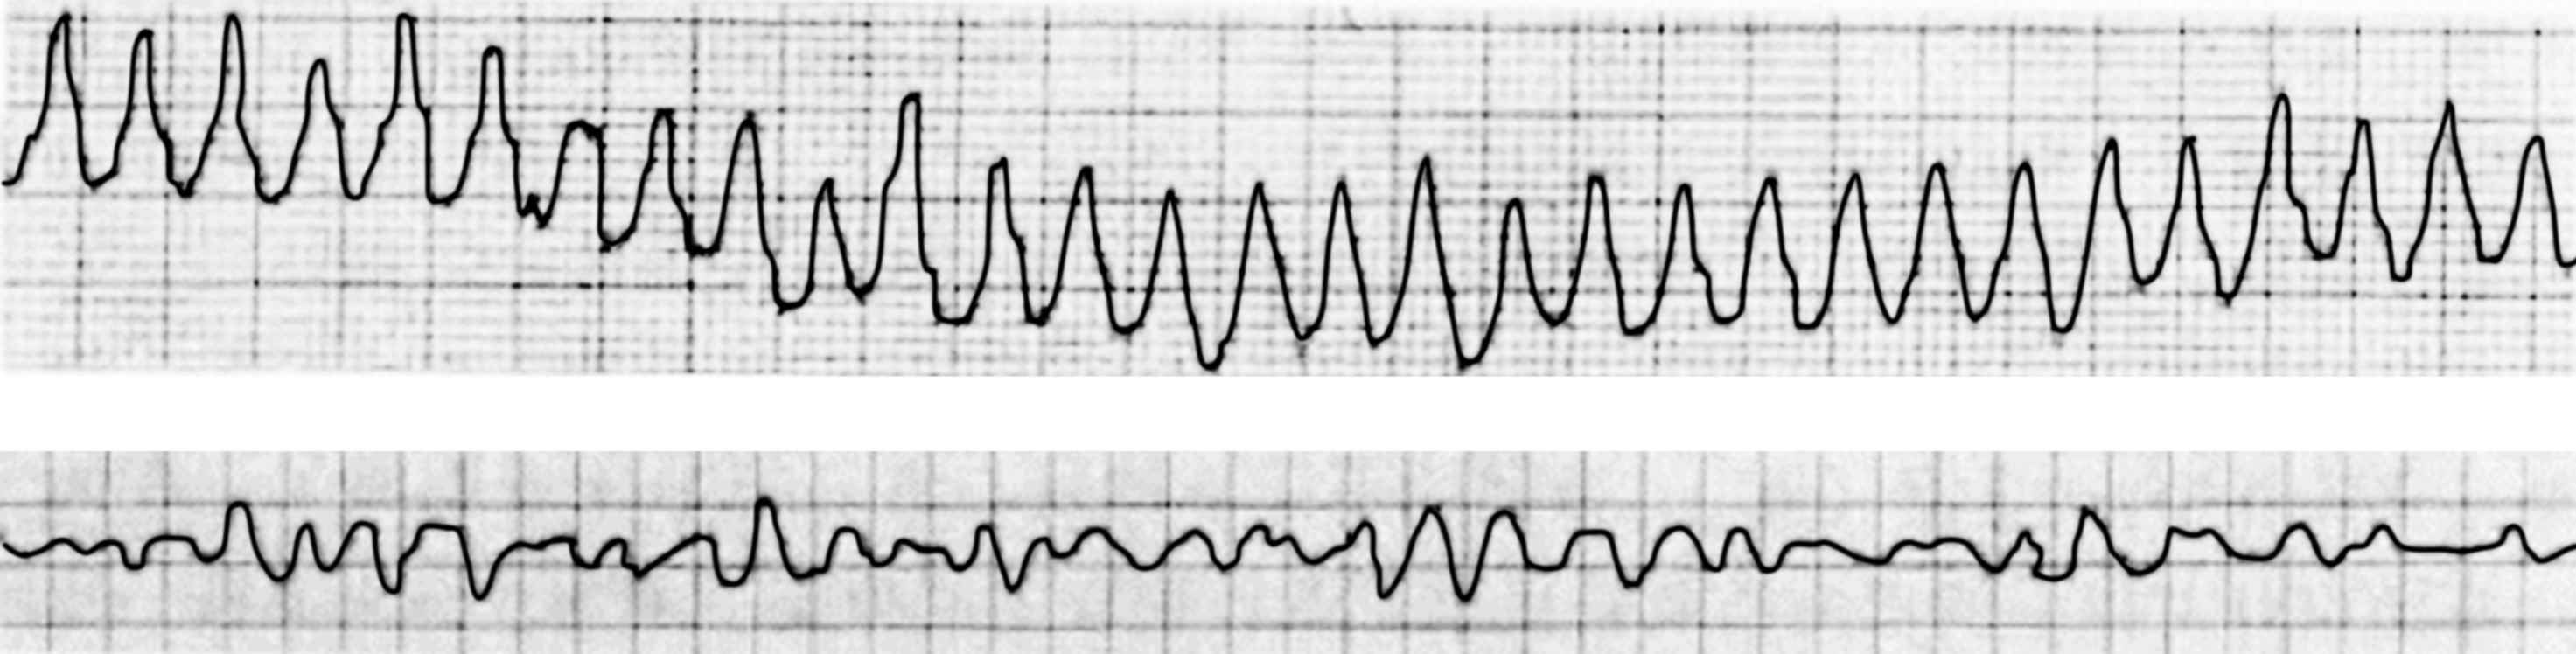
\includegraphics[width=6.29167in,height=1.59375in]{./images/Image00458.jpg}
 \captionsetup{justification=centering}
 \caption{心室扑动(上)和心室颤动(下)}
 \label{fig102-19}
  \end{figure} 

2. American Heart Association. 2010 American Heart Association
Guidelines for Cardiopulmonary Resuscitation and Emergency
Cardiovascular Care. Circulation,2010,122(suppl 3):S640-S767

\protect\hypertarget{text00297.html}{}{}

\section{房室传导阻滞}

房室传导阻滞(atrioventricular
block,AVB)是指激动从心房传到心室的过程中,任何部分发生传导延迟或受到阻滞,以致激动部分或完全不能到达心室。是一种最常见的心脏传导阻滞。

关于AVB的分类,按照病程可分为急性和慢性AVB,慢性AVB还可以分为间断发作型与持续发作型;按照病因可分为先天性与后天性AVB;按照阻滞部位可分为房室束分支以上与房室束分支以下阻滞两类,其病因、临床表现、发病规律和治疗各不相同;按阻滞程度可分为不完全性与完全性AVB:根据阻滞的程度传统上分为一、二、三度,一度:全部激动均能由心房传至心室,但传导时间延迟,阻滞部分多在房室结以上;二度:部分激动不能传至心室,又分为Ⅰ型(莫氏Ⅰ型)和Ⅱ型(莫氏Ⅱ型);三度:激动均不能下传到心室。从临床角度看,按阻滞程度和阻滞部位分类不但有利于评估阻滞的病因、病变范围和发展规律,还能指导治疗。

二度以上AVB,由于心室搏动脱漏可有心动过缓及心悸、胸闷症状,高度或完全性AVB时严重心动过缓可致心源性晕厥,均构成急症。

\subsection{病因与发病机制}

\subsubsection{病因}

导致AVB的常见病因为:AMI、冠状动脉痉挛、病毒性心肌炎、心内膜炎、心肌病、急性风湿热、钙化性主动脉瓣狭窄、心脏肿瘤(特别是心包间皮瘤)、先天性心血管病(原发或继发孔型房缺、室缺、完全性大血管异位伴单心室、肺动脉发育不良等或AVB为唯一先天性异常)、原发性高血压、心脏外科手术(主要是室间隔缺损修补术后)、电解质紊乱(高钾血症最常见)、药物中毒(洋地黄、奎尼丁、普鲁卡因胺、维拉帕米等)等。Lev病(心脏纤维支架的钙化与硬化)与Lenegre病(传导系统本身的原发性硬化变性疾病)可能是成人孤立性慢性心脏传导阻滞最常见的原因。少数正常人或运动员可发生莫氏Ⅰ型AVB,PR间期0.22~0.24秒而无心脏病证据,与迷走神经张力增高有关,常发生于夜间。由希氏束分叉以上阻滞的AVB病情较轻,而希氏束分叉以下由双束支或三支阻滞引起的AVB,多半为心肌弥漫性病变同时有双支或三支广泛损害,病情较重。如广泛心肌梗死、心肌炎、心肌病等。

\subsubsection{发病机制}

一度和二度Ⅰ型AVB,阻滞部位多为房室结,病理改变多不明显或为暂时性房室结缺血、缺氧、水肿、轻度炎症,药物过量如洋地黄、β受体阻滞剂、钙拮抗剂及训练有素运动员等使迷走神经过度紧张所致。

二度Ⅱ型AVB和双侧或三支阻滞,病理组织改变常广泛而严重,包括传导系统的炎症或局限性纤维化,广泛前壁心肌梗死累及希氏束,左右束支分叉处或双侧束支坏死及束支广泛纤维性变。成人传导系统变性多由于Lev病或Lenegre病所致,前者为心脏纤维支架的钙化和硬化,常累及主动脉瓣、二尖瓣、中央纤维体和室间隔顶部;后者为传导系统本身的原发性硬化变性,不累及心肌和心脏纤维支架。此两种病可能是成人孤立性慢性房室阻滞最常见的病因,常伴束支阻滞。此外,先天性完全性AVB,可见房室结或希氏束的传导组织完全中断或缺如。

不同病因引起的AVB可有不同的阻滞部位、阻滞程度和发展规律(表\ref{tab102-18})。

\subsection{诊断}

\subsubsection{临床表现特点}

一度AVB通常无症状,听诊时因PR间期延长,第一心音强度减弱。二度AVB可引起心搏脱漏,可有心悸症状,也可无症状;听诊时二度Ⅰ型第一心音强度逐渐减弱并有心搏脱漏,二度Ⅱ型亦有间歇性心搏脱漏,但第一心音强度恒定。三度AVB的症状取决于心室率的快慢与伴随病变,属先天性者其心室率较快,休息时可无症状,仅于活动时感心悸、气喘;其他原因引起者心室率较慢,患者自觉心率缓慢、心跳强而有力;心室率过慢时则有心悸、气喘、胸闷、头晕、乏力等,重者可出现阿斯综合征或心力衰竭;体检心率缓慢规则,多在30~40次/分(先天性者可达50~60次/分),运动后并不相应地增快,心尖第一心音响度强弱不等,有所谓“大炮音”(在房室同时收缩时,第一心音特别响亮),颈静脉有强弱不等搏动(因房室同时收缩造成强的搏动),且其频率较心室率明显快。脉搏强,脉压大,血压高低不等波动大。

\subsubsection{心电图特点}

\hypertarget{text00297.htmlux5cux23CHP10-2-10-2-2-1}{}
(一) 一度 AVB

一度AVB(first degree A-V block)仅表现为PR间期延长,成人>
0.20秒,儿童>
0.16~0.18秒,PR间期一般时间为0.21~0.40秒。PR间期明显延长时,P波可隐伏在前一个心搏的T波内,引起T波增高、畸形或切迹,或延长超过PP间距,而形成一个P波越过另一个P波传导,后者多见于快速性房性异位心律。显著窦性心律不齐伴一度AVB时,PR间期可随其前的RP间期的长或短而相应地缩短或延长。

一度AVB还可分为三型:Ⅰ型为PR间期逐渐延长后又逐渐减轻,并周而复始;Ⅱ型为PR间期延长固定不变;Ⅲ型为PR间期延长无一定规律。

希氏束电图特征:①心房内阻滞:P-A间期>
60ms,而A-H、H和H-V间期均正常。②房室结内阻滞:A-H延长>
140ms,P-A和H-V间期正常。③希氏束内阻滞:H-H′间期延长>
20ms。④束支阻滞:H-V间期延长> 60ms。

\hypertarget{text00297.htmlux5cux23CHP10-2-10-2-2-2}{}
(二) 二度 AVB

二度AVB(second degree A-V
block),即“不完全性房室传导阻滞”。若心电图显示若干个窦性P波后未继以QRS波群,且排除干扰现象,即可称为二度AVB。二度AVB患者自觉症状与心室率的快慢有关:当阻滞所致心室漏搏只偶尔出现时,患者可无自觉症状,或仅感心悸;如心室漏搏频繁而致心室率甚慢时,则可有乏力、头晕、心慌等症状,甚至发生阿-斯综合征;体检发现心音和脉搏脱漏。

\begin{table}[htbp]
\centering
\caption{房室传导阻滞的病因、病理变化、阻滞部位、阻滞程度和发展规律之间的关系}
\label{tab102-18}
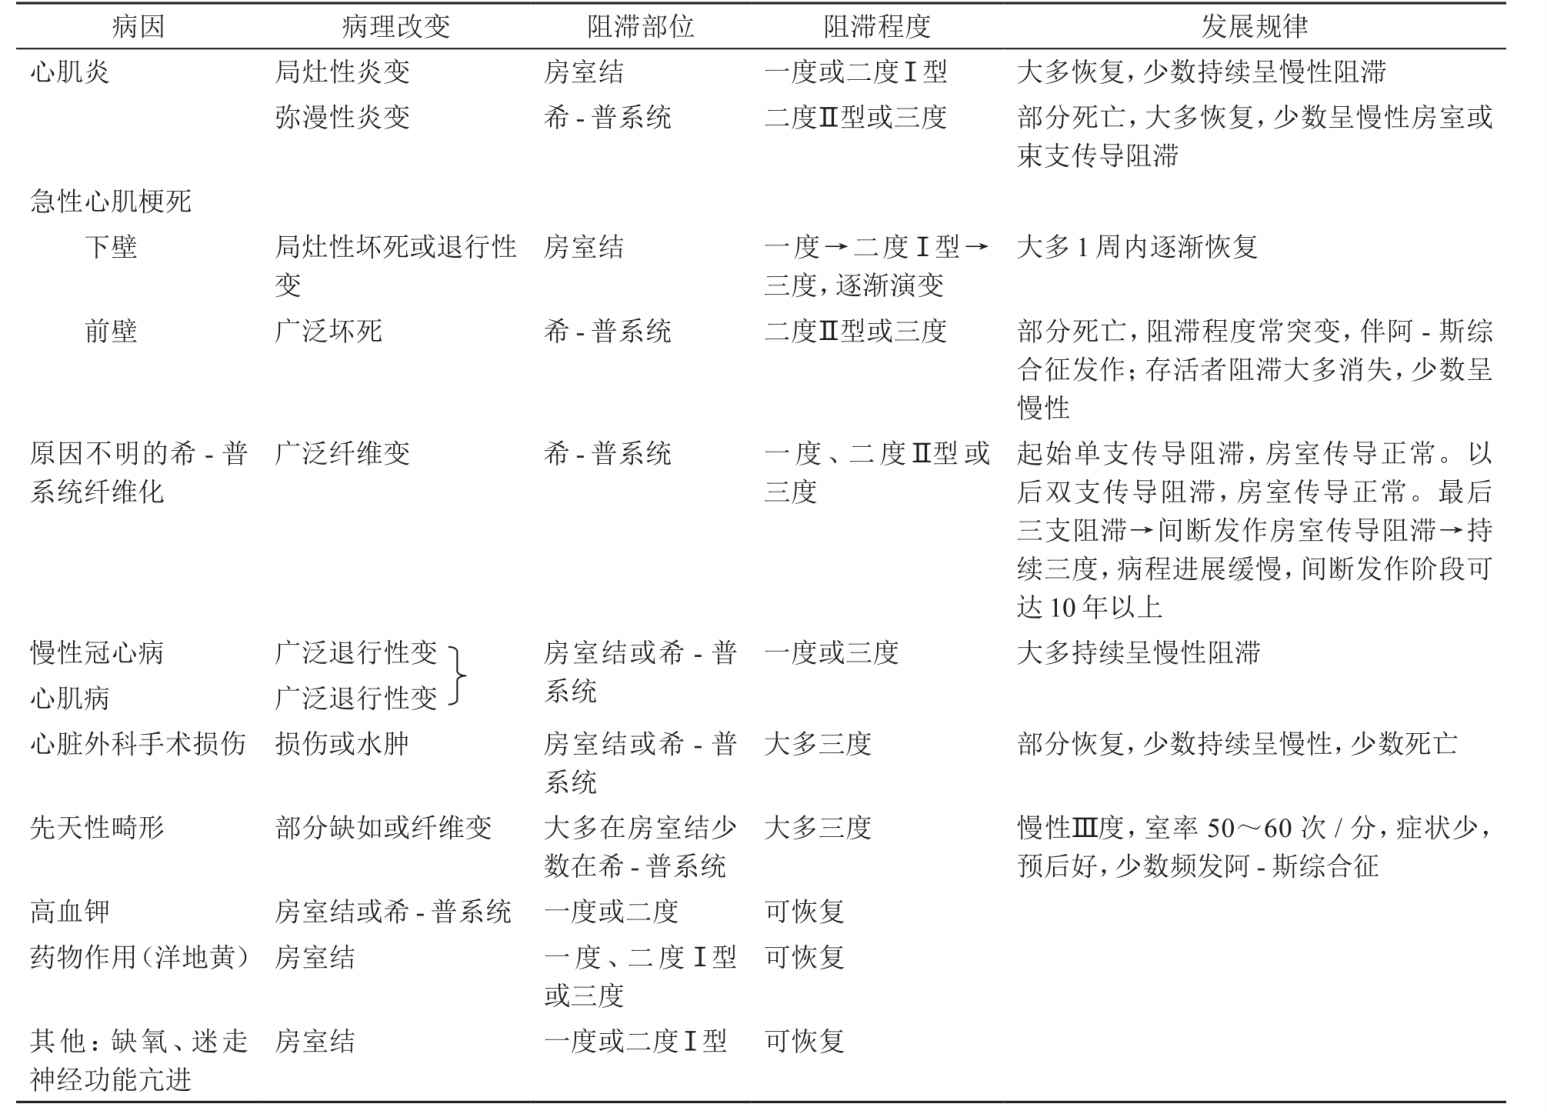
\includegraphics[width=6.69792in,height=4.82292in]{./images/Image00459.jpg}
\end{table}

二度AVB按阻滞的程度分为莫氏Ⅰ型(MobitzⅠ型)和莫氏Ⅱ型(MobitzⅡ型)。

\paragraph{MobitzⅠ型AVB}

莫氏Ⅰ型又称文氏阻滞,是最常见的二度AVB类型,多数情况下阻滞位于房室结,QRS波群正常,极少数可位于希氏束下部,QRS波群呈束支传导阻滞图形。心电图特点是:①PR间期进行性延长,直至一个P波受阻不能下传心室。②相邻RR间期进行性缩短,直至一个P波不能下传心室。③包含受阻P波在内的RR间期小于正常窦性PP间期的2倍。最常见的房室传导比例为3∶2和5∶4。

希氏束电图特征:80\%的阻滞部位在希氏束近端,A-H间期进行性延长,直至完全阻滞,H-V间期正常。若希氏束本身或远端阻滞,则H-H′或H-V间期逐渐延长而至完全阻滞。

具有典型文氏现象的二度Ⅰ型AVB仅占50\%左右,出现以下心电图现象,提示非典型文氏现象或变异型文氏现象:①非典型文氏现象:PR间期的增量逐渐增大;PR间期逐搏延长后QRS漏搏;文氏周期第一个R-R间期<最后一个R-R间期;P-P间期最短时P-R间期增量最大等。②变异型文氏现象:PR间期增量不一;有≥2个相等的PR间期或R-R间期;每次文氏周期的最后一个R-R不是最短者;QRS漏搏引起的长R-R间期大于两个短R-R间期之和等。

\paragraph{MobitzⅡ型AVB}

本型可与二度Ⅰ型AVB交替转换,为房室传导呈比例的中断,房室结及房室结以下传导阻滞分别为38\%和62\%,常见于广泛不可逆的器质性心脏病和高血钾,房室传导系统的病理性的绝对不应期延长,延长的绝对不应期间歇超过一个心房的心动周期,使下一个P波受阻,QRS波群漏搏一次。相对不应期不延长表现为PR间期正常。心电图特点:①PR间期固定,可正常或延长,心室脱漏搏动前后的PR间期不改变。②QRS波群呈周期性脱漏,房室传导比例可为2∶1,3∶1,3∶2,4∶3,5∶4等。③下传QRS波群多呈束支传导阻滞型。二度Ⅱ型AVB中,房室呈3∶1或3∶1以上比例的,称为高度AVB;若绝大多数P波后无QRS波群,心室基本由房室交界处或心室自主心律控制的,称为近乎完全性AVB。

希氏束电图特征:①多为希氏束远端阻滞,A-H间期正常,H-V间期延长;未下传心搏的H波后无V波。②少数希氏束近端阻滞者A-H延长,下传的H-V间期正常;未下传A波后无H波和V波。

二度Ⅰ型和Ⅱ型AVB的鉴别见表\ref{tab102-19}。

\paragraph{二度 AVB诊断中的若干问题}

(1)
任何室上性心律均可合并二度AVB。窦性心律不齐合并二度Ⅰ型AVB可使文氏现象不典型;心房扑动的心房率常因二度AVB,多呈2∶1下传而使心室率在150次/分左右;阵发性房性心动过速可伴程度不等的二度AVB而使心室律不齐。

\begin{table}[htbp]
\centering
\caption{二度Ⅰ型与二度Ⅱ型AVB的鉴别}
\label{tab102-19}
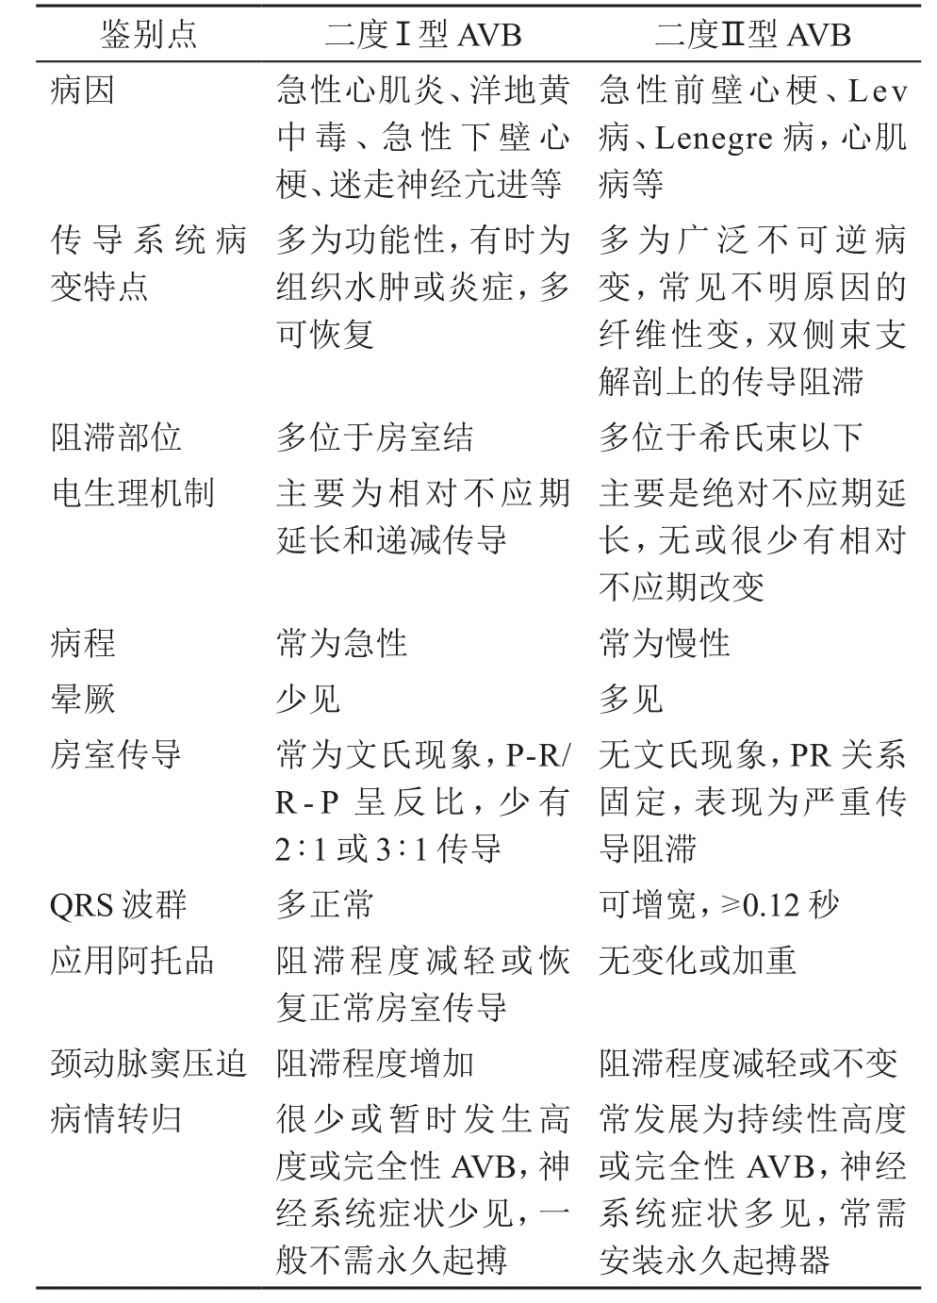
\includegraphics[width=3.30208in,height=4.59375in]{./images/Image00460.jpg}
\end{table}

(2) 交替性文氏周期(alternating Wenckebach
period):指在2∶1房室传导时,下传心搏的PR间期逐渐延长,最后脱漏,以连续2~3个P波连续下传受阻而结束一个文氏周期。其可发生于房结区、结区及结希区中存在两个功能与水平不同的阻滞区。若结区为文氏传导,房结区或结希区为2∶1传导,称为A型交替性文氏传导;若结区为3∶2文氏传导和结希区为2∶1传导,则为B型交替性文氏传导。可见于急性下壁心梗、传导系统原发性病变、心房扑动、伴AVB的房速等。

(3)
连续2个或数个P波未下传心室,房室传导比例为3∶1或4∶1,伴逸搏与逸搏心律、夺获心搏,称为高度房室传导阻滞(high
grade A-V
block)。二度AVB合并隐匿性传导为原因之一,可发生在窦性心律、房性异位心律或交界性心律的基础上,为二度AVB中较严重的一种,常是发生完全性AVB的前奏,临床意义等同于完全性AVB。

(4)
部分二度AVB与二度Ⅰ型或Ⅱ型AVB均不甚相同时,称Ⅲ型AVB,心电图特征为:①PR间期波动与迷走神经改变有关;②生理部分阻滞型心室漏搏下传PR间期长短不一。

(5)
心率加快至一定限度时即出现PR间期正常和心室漏搏,心房率减慢时阻滞消失者,为3相二度Ⅱ型AVB。心率减慢后即出现二度Ⅱ型AVB,心房率正常则阻滞消失,为4相二度Ⅱ型AVB。

(6)
持续2∶1传导的AVB是二度AVB的一种特殊类型,因它既可是二度Ⅰ型也可是二度Ⅱ型,如同时见有束支传导阻滞或有3∶2房室传导,则常为二度Ⅱ型(希氏束下阻滞);如QRS波正常,则常提示为二度Ⅰ型(房室结阻滞)。

\hypertarget{text00297.htmlux5cux23CHP10-2-10-2-2-3}{}
(三) 完全性 AVB

完全性房室传导阻滞(complete A-V
block),又称三度AVB,其特点为房室交界区有适合的传导条件,但全部室上性激动均因阻滞而不能传到心室。发生机制与房室传导系统绝对不应期延长、心脏手术并发的房室传导系统连续中断、先天性完全性AVB、射频消融损伤房室结等有关。三度AVB中,属先天性者其心室率较快,休息时可无症状,仅于活动时感心悸、气喘;其他原因引起者心室率较慢,患者自觉心率缓慢、心跳强而有力;心室率过慢时则有心悸、气喘、胸闷、头晕、乏力等,重者可出现阿斯综合征或心力衰竭;体检心率缓慢规则,多在30~40次/分(先天性者可达50~60次/分),运动后并不相应地增快,心尖第一心音响度强弱不等,有所谓“大炮音”(在房室同时收缩时,第一心音特别响亮),颈静脉有强弱不等搏动(因房室同时收缩造成强的搏动),且其频率较心室率明显快。脉搏强,脉压大,血压高低不等波动大。

心电图特点:三度AVB时,全部P波不能下传,P波与QRS波群无固定关系,形成房室脱节,二者有各自的频率,前者多在60~100次/分,后者多在30~50次/分。心室由低位起搏点激动控制,QRS波群形态与频率依赖于异位起搏点的位置:心室起搏点发生在房室束分支以下,为心室自主心律,QRS波群增宽畸形,时限>
0.12秒,心室率多甚慢仅30~40次/分;心室起搏点发生在房室束分支以上或之内为房室交界处性心律,QRS波群形态与时限均正常,心室率不太慢在50次/分左右。双侧束支或三束支传导阻滞所引起的Ⅲ度AVB,其QRS波群可时而呈右束支传导阻滞型,时而呈左束支传导阻滞型,有时可在心电图上出现短暂的心室停顿而至R-R间期不等,或一系列的P波后无QRS波群,也可发生VF。

希氏束电图特征:①希氏束近端完全阻滞------A-H阻滞:A波后无H波,V波前有H波,H-V固定,A波与V波无固定关系。②希氏束内阻滞------A波后有H波,A-H固定且正常,A波与V波无关,H-H′中断,每个V波前有H′波,V波正常。③希氏束远端阻滞------H-V阻滞:A波后有H波,A-H间期固定,但H波不能下传,其后无V波。

三度AVB阻滞部位的定位见表\ref{tab102-20}。

\subsubsection{AVB的定位}

\paragraph{希氏束电图(HBE)对AVB的定位}

见表\ref{tab102-21}。

\paragraph{心电图对 AVB的定位}

大多数AVB病例可根据常规心电图对希氏束分支以上部位的阻滞或分支以下部位的阻滞作出判断,见表\ref{tab102-22}。

\paragraph{阿托品试验对 AVB的定位}

\hypertarget{text00297.htmlux5cux23CHP10-2-10-2-3-3-1}{}
(1) 一度AVB:

如阻滞在房室结水平,则静注阿托品1~2mg可使阻滞消失;如阻滞在希氏束水平,则静注阿托品(或心房调搏)心率加快后保留一度AVB,或形成二度AVB加束支阻滞。

\hypertarget{text00297.htmlux5cux23CHP10-2-10-2-3-3-2}{}
(2) 二度AVB:

如阻滞在房室结水平,则静注阿托品1~2mg,文氏现象可消失;如阻滞在希氏束水平,则静注阿托品后可使AVB加重,有发展为三度AVB之可能;少数表现为文氏现象,但阿托品不易消除之。

\begin{table}[htbp]
\centering
\caption{三度 AVB不同阻滞部位的特征比较}
\label{tab102-20}
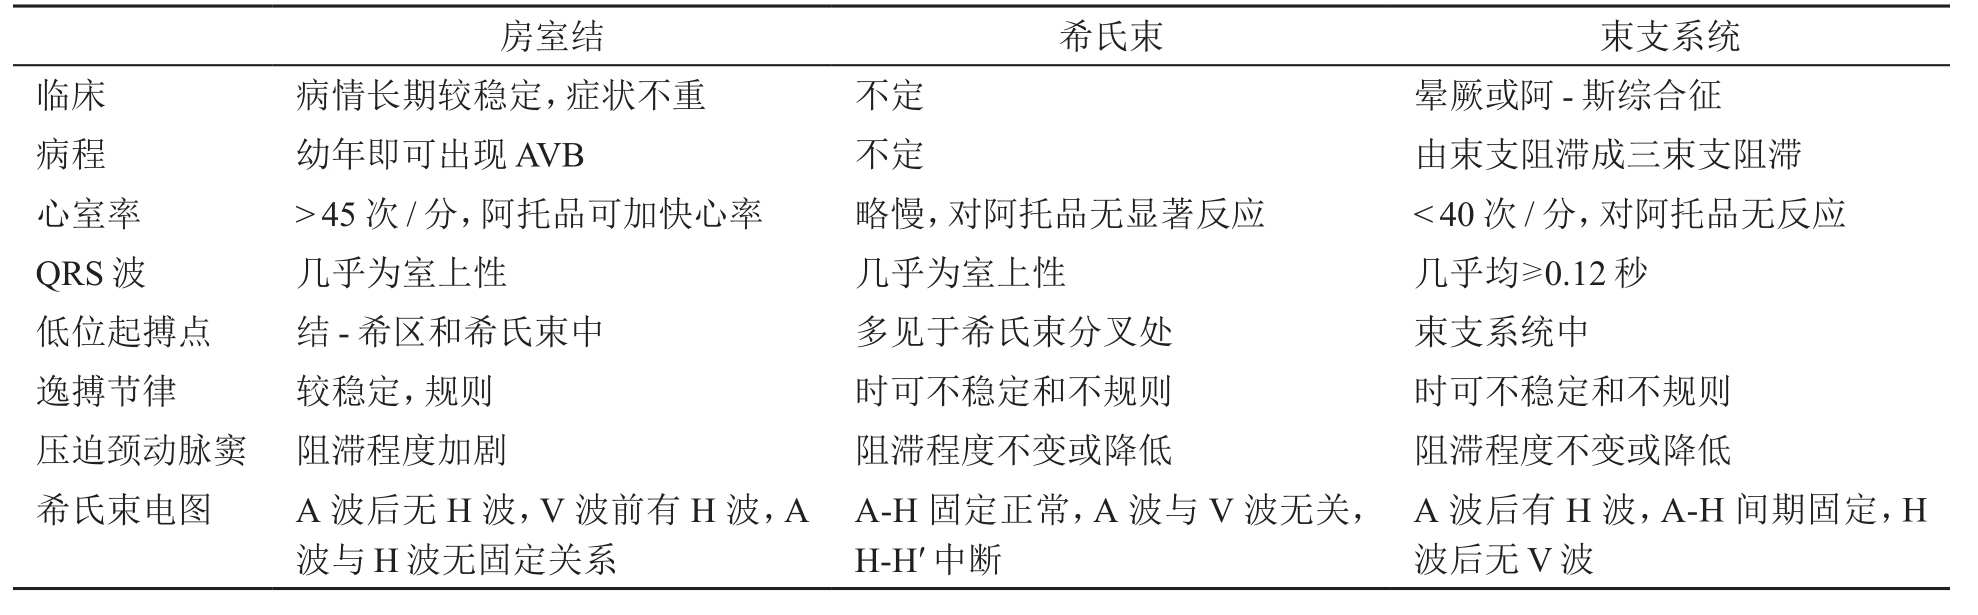
\includegraphics[width=6.58333in,height=2.04167in]{./images/Image00461.jpg}
\end{table}

\begin{table}[htbp]
\centering
\caption{希氏束电图对 AVB的定位}
\label{tab102-21}
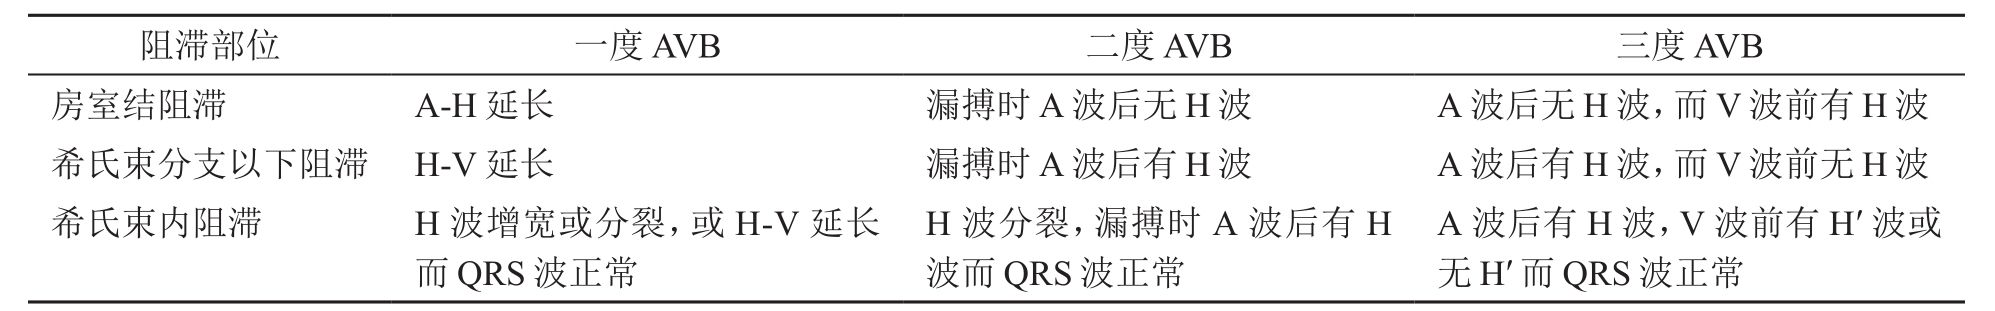
\includegraphics[width=6.64583in,height=1.02083in]{./images/Image00462.jpg}
\end{table}

\begin{table}[htbp]
\centering
\caption{心电图对 AVB的分型与定位}
\label{tab102-22}
\includegraphics[width=3.25in,height=1.95833in]{./images/Image00463.jpg}
\end{table}

二度Ⅱ型结区阻滞常与交界处隐匿性冲动形成或折返有关

\hypertarget{text00297.htmlux5cux23CHP10-2-10-2-3-3-3}{}
(3) 三度AVB:

如阻滞在房室结水平,则静注阿托品1~2mg可部分恢复房室传导,此种房室结水平阻滞多见于心肌炎、急性下壁梗死及洋地黄过量等。如阻滞在希氏束水平,则静注阿托品无效。但静注20分钟内,如逸搏频率明显增加(>
9次/分)常提示为希氏束近端阻滞;如逸搏频率不变或增快5次/分以下者,提示为希氏束远端阻滞。如逸搏QRS波宽,则用药后频率明显增快者,提示希氏束近端阻滞合并束支阻滞;而用药后逸搏频率不变或仅微增加者,提示希氏束远端阻滞合并束支阻滞。

\subsection{治疗}

AVB尤其是二度AVB以上者的治疗原则是治疗原发病,提高心室率,起搏器治疗。

\subsubsection{病因治疗}

应针对不同的病因进行治疗。如用抗生素治疗急性感染,阿托品解除迷走神经张力增高,停用导致AVB的药物,纠正电解质紊乱等。各种急性心肌炎、心脏直视手术损伤或急性下壁心肌梗死等引起的AVB,可用氢化可的松200~300mg或地塞米松10~20mg,加入5\%葡萄糖液500ml中静滴,取得疗效后改用泼尼松(强的松)10~20mg口服,每日3次;待传导阻滞程度减轻或消失后,逐渐减量,最后停药。

\subsubsection{提高心室率}

一度与二度Ⅰ型AVB,心室率≥50次/分,无明显症状者,一般无需特殊处理。二度Ⅱ型和三度AVB从未发生过阿-斯综合征者,可酌情选用下列药物或措施提高心室率,促进传导,以防阿-斯综合征发作,尤其是心室率<
50次/分,有明显症状者。

\paragraph{阿托品}

可解除迷走神经对心脏的抑制作用,使心率加快,一般情况下不增加心肌的耗氧量。适用于希氏束分支以上的阻滞。可用阿托品0.3~0.6mg口服,或0.5~1.0mg静脉或肌内注射,4~6小时一次。但应注意,阿托品虽能加速房室传导纠正文氏现象,但它加快心房率,可使二度Ⅱ型AVB加重,尤其QRS波宽大畸形者不宜应用。亦可选用山莨菪碱等药物。

\paragraph{麻黄碱}

对α及β受体均有兴奋作用,升压作用弱而持久,并有加快心率作用。适用于二度或三度AVB症状较轻患者。可用麻黄碱25mg,每6~8小时1次口服。亦可用沙丁胺醇(舒喘灵)2.4~4.8mg口服,每日3次。

\paragraph{异丙肾上腺素}

可用10mg舌下含服,每4~6小时1次,必要时需用0.5~1.0mg加入5\%葡萄糖液500ml中持续静滴,控制滴速使心室率维持在60~70次/分;过量不仅可明显增快心房率而使房室阻滞加重,而且还能导致严重室性异位心律。

\paragraph{碱性药物(5\%碳酸氢钠或克分子乳酸钠)}

有改善心肌细胞应激性,促进传导系统心肌细胞对拟交感神经药物反应的作用,尤适用于高血钾或伴酸中毒时。

\subsubsection{起搏器治疗}

二度Ⅱ型AVB有明显缺血症状或经上述药物治疗病情不好转者,或三度AVB有晕厥及阿-斯综合征发作者应植入起搏器。若估计为暂时性严重AVB,可先植入临时起搏器,积极治疗原发病,观察变化。若由慢性双侧束支或三束支阻滞引起三度AVB,心室率25~40次/分,QRS波宽大畸形,节律点不稳定,应考虑植入永久性起搏器治疗。

\hypertarget{text00297.htmlux5cux23CHP10-2-10-4}{}
参 考 文 献

1. 曹林生 ,廖玉华.心脏病学.第3版.北京:人民卫生出版社,2010:387

2. 陈灏珠 ,林果为.实用内科学.第13版.北京:人民卫生出版社,2009:1420

\protect\hypertarget{text00298.html}{}{}

\section{病态窦房结综合征}

病态窦房结综合征(sinus sick
syndrome,SSS),简称病窦,是心源性昏厥的主要原因之一,是一组心血管系统比较常见的严重疾病。它是由多种病因引起的窦房结本身及其周围组织病变,造成心脏起搏和传导功能失常,从而产生一系列的心律失常、血流动力学障碍和心功能受损,严重者可发生阿-斯综合征(Adams-Stokes
syndrome)甚至猝死。

1967年
Lown在总结心律失常电复律的并发症中,认为不能恢复维持窦性心律的患者可能有窦房结起搏传导功能异常,并首先提倡用病态窦房结综合征一词。1968
年Ferrer认为下述情况应属于病态窦房结综合征:①持久的、严重的和难以预料的窦性心动过缓;②短时间窦性停搏伴有房性或交界区心律;③长时间的窦性停搏,引起心跳停止或室性心律失常;④一过性或慢性心房颤动伴缓慢心室率且可以排除药物所致;⑤心房颤动经电复律后,不能恢复窦性心律;⑥与药物无关的窦房传导阻滞。1972年Ruben-stein将病态窦房结综合征分为3组:①心动过缓;②窦性停搏或窦房传导阻滞;③心动过缓、窦性停搏或窦房传导阻滞同时并发室上性心动过速、心房扑动或心房颤动,即心动过缓-心动过速综合征。

病窦是由多种原因引起的一组临床综合征,而不是一种疾病。发病率在一般人群中并不清楚,然而无症状性窦房结功能异常很常见,据报道,正常儿童中有65\%存在窦房传导阻滞,在男性医学生中有28\%存在窦房传导阻滞,在动态心电图中有1.4\%的中年男性有窦房传导阻滞,在综合性医院行12导联心电图者中有0.4\%窦性心动过缓或窦性停搏。从几项植入永久性心脏起搏器的统计数据来看,此类患者在临床上较多见。1981年《世界心脏起搏述评》中指出:植入永久性心脏起搏器者中52\%是病窦。由中华医学会心电生理与起搏分会和中国生物医学工程学会心脏节律分会共同组织的对2002~2005年全国心脏起搏器临床应用调查结果表明,在植入永久性心脏起搏器者中50.1\%~52.0\%是病窦患者。虽然任何年龄均可发病,但以老年人多见,其病程发展大多缓慢,从首次发病到症状严重可长达5~10年或更长;少数呈急性发作,见于急性心肌梗死或急性心肌炎。病窦患者常以各种类型心律失常就诊,极易导致误诊误治,临床上应引起重视。

\subsection{窦房结的解剖生理特点}

窦房结是心脏的起搏点,正常节律性冲动的发源地。由英国的Keith和Flack于1907年首次在哺乳动物中发现,1910年由Wybouw和Lewis等首次描述了它作为心脏起搏点的电生理特性。通常位于右心房的上腔静脉入口处界嵴的上端,形如带壳的蜗牛,长10~20mm,宽厚2~3mm,尾端向下腔静脉逐步变狭,位于心外膜下1mm处。窦房结有丰富的自主神经(交感神经和迷走神经)末梢并与窦房结细胞直接接触(具有神经-肌肉接头结构),便于对窦房结电活动的频率、节律起调节作用。窦房结主要受右侧迷走神经和交感神经丛的控制,这与房室结构明显不同。其解剖生理具有以下一些特点。

\paragraph{细胞组成}

窦房结由P细胞、T细胞和心房肌细胞组成:①起搏细胞(pacemaker
cell):又称P细胞或窦房结细胞,位于窦房结中央,因肌原纤维少,不具收缩功能,形态圆小(5~10μm)、色淡苍白、分化程度低,类似原始心肌细胞,只发放冲动,具有自动起搏的特性,维持心脏节律性活动。随着年龄的增加,窦房结内的P细胞逐渐减少,脂肪组织和弹力纤维逐渐增多,一些老年人的起搏功能可能降低P细胞受损,窦房结自律性降低或冲动形成障碍。②过渡细胞(transition
cell):又称T细胞、移行细胞,位于P细胞周围,连接P细胞与心房肌细胞,肌原纤维较多,具有传递冲动的功能。在T细胞和心房肌细胞之间,存在着发育更充分的闰盘是窦房结内发出的冲动传导至心房的通路。过渡细胞受损,易发生传出阻滞,即窦房传导阻滞。

\paragraph{血液供应}

①窦房结由心房中最粗大的窦房结动脉供血,约60\%起源于右冠状动脉,40\%起源于左旋支,绝大部分为单支供血,极少数为双支供血。②窦房结动脉因多数来自右冠状动脉。故右冠状动脉阻塞所致心肌梗死者,5\%可伴病窦。因窦房结动脉发自右冠状动脉主干较早,故伴急性病窦者,说明右冠状动脉阻塞位置较高,梗死面积较大。前侧壁心肌梗死合并窦房结功能不全者,表明左旋支近端1~2cm内有阻塞。③窦房结动脉阻塞的后果为:窦房结和心房肌的营养灌注受损;冠状动脉之间的重要吻合途径中断;伺服机制(servomechanism)丧失。

大量研究表明,中国人的窦房结动脉约57\%起自右冠状动脉近端1~2cm处,39.3\%起自左冠状动脉旋支近端1cm之内。它们分别以顺时针或逆时针方向沿上腔静脉右心房交界到达窦房结,2.9\%可以从左、右冠状动脉双侧发出。

\paragraph{窦房结动脉的生物学意义}

窦房结动脉横贯窦房结中央,结内小动脉管径所占面积8倍于心房壁小动脉的分布,其与窦房结细胞之间,存在着密切的组织功能联系,以保证其起搏功能所需。当心跳停止,作心脏按压时,窦房结动脉扩张,刺激周围P细胞,使之除极并发放冲动,心脏得以复苏,即谓伺服机制。逸搏-夺获亦属于这一范畴。

\subsection{病因与发病机制}

一般认为病窦的病因以冠心病最常见,约占50\%,但此观点存在异议。根据近年一些文献报道,在对病窦患者行冠状动脉造影的调查中,发现冠状动脉狭窄≥50\%的仅占15\%~48\%;国外病理调查报告2/3的病窦患者窦房结血管无异常发现。不少学者对传导系统增龄变化的病理学进行研究并证实,随着年龄的增长,窦房结内逐渐纤维化,起搏细胞被纤维组织取代,继之窦房结功能逐渐衰退。所以除可能与传导系统慢性缺血有关外,更多的原因是由于传导系统退行性病变。

许多因素可引起病窦综合征,但部分患者为特发性。窦房结组织纤维性退化是导致病窦最常见的内在因素,一些外源性因素也可导致窦房结功能障碍。按病程长短,可将病窦分为急性和慢性两类,每类又有器质性和功能性两种原因,具体见表\ref{tab102-23}。

有相当数量的患者是冠心病和病窦同时存在。尽管冠心病不是病窦的主要原因。心梗患者是否由于炎症、窦房结缺血、或局部自主神经作用导致病窦综合征尚不清楚。急性心肌梗死引起的窦房结功能紊乱通常是短暂的。不常见的是急性心肌梗死后慢性缺血致纤维化且出现病窦症状,持续数月到数年。

病理上,主要表现为窦房结细胞的显著减少与纤维组织的大量增生,以及窦房结动脉、窦房结周围和心房组织,甚至房室结区和希-普系统的病变。疾病初期窦房结功能、起搏/传导细胞损伤较轻,伴随着窦房结细胞不断减少和纤维组织的不断增多,窦房结功能由间歇性降低演变为持续性障碍,从而导致心脏下部起搏点发出逸搏,若不能发出,常因心脏停搏而引起急性心源性脑缺血综合征。

病理生理基础主要为窦房结冲动形成异常和传出障碍,以及由此而诱发的代偿性房性心律失常,同时伴有房室结、希-普系统功能障碍。

因迷走神经张力异常增高,明显抑制窦房结功能,导致过缓性心律失常,伴有一系列症状。这种窦房结以外因素造成窦房结功能障碍,称为结外病态窦房结综合征。其特点为患者较年轻,有晕厥史,出现快速心律失常、伴器质性心脏病、慢-快综合征及双结病变者明显少于结内组,多数无器质性心脏病,药物阻滞后可缩短延长的电生理参数,系迷走神经张力异常增高所致,属功能性改变。而结内组窦房结及其周围组织器质性病变伴器质性心脏病较多,药物阻滞前后电生理参数无明显差异,属器质性病变(表\ref{tab102-24})。

\subsection{诊断}

\subsubsection{临床表现特点}

发病年龄以老年人居多,这可能与人体窦房结的胶原和弹力纤维随年龄增高而增多有关。但家族性病窦患者却可在婴儿或儿童时期就发病。病窦患者出现临床症状的平均年龄约为65岁。

\begin{table}[htbp]
\centering
\caption{病态窦房结综合征的病因和分类}
\label{tab102-23}
\includegraphics[width=6.67708in,height=4.84375in]{./images/Image00464.jpg}
\end{table}

\begin{table}[htbp]
\centering
\caption{两种病态窦房结综合征临床和电生理特点}
\label{tab102-24}
\includegraphics[width=3.23958in,height=2.77083in]{./images/Image00465.jpg}
\end{table}

病窦病程较长,发展缓慢,可持续5~10年或更长,早期起搏传导组织受损较少、较轻,可无症状或间歇出现症状,临床表现不典型,早期诊断困难。随着病程进展,窦房结细胞不断减少,纤维组织不断增加,可呈严重而持久的窦性心动过缓、较长的窦性停搏、频发窦房传导阻滞,可出现重要脏器供血不足的表现。

\paragraph{中枢神经系统症状}

表现为头晕、健忘、反应迟钝、瞬间记忆障碍,进一步发展可有黑矇、眩晕(6\%~11\%)、晕厥(40\%~80\%),甚至阿-斯综合征。一般均由严重的窦性心动过缓或停搏所致,慢-快综合征者的晕厥半数是由心动过缓的转变过程中伴有长间歇所致,缘于快速心律对窦房结的超速抑制。

\paragraph{心血管系统症状}

主要表现为心悸。无论过缓、过速或不齐,患者均可感到心悸。过缓者由于每搏量增加,有心跳沉重感。过速者因心率加快而感到心悸。快慢不齐者,心悸更加明显。慢-快综合征快速性房性心律失常持续时间长者,易致心力衰竭。有冠心病基础者,可诱发心绞痛。一般规律显示,过速转为过缓,停搏时间长者,可发生晕厥、阿-斯综合征。过缓转为过速,则可出现心悸、心绞痛、心力衰竭加重。

\paragraph{肾脏和胃肠道症状}

由于过缓-过速性心律失常,导致心排血量降低,以致肾血流量降低,可表现尿量减少,胃肠道供血不足表现为食欲不振、吸收不良、胃肠道不适等。

\subsubsection{常规心电图特点}

病窦患者可有各种异常的心电图表现,主要包括:

1.窦性心动过缓 最早,最常见,占病窦的60\%~80\%。心率多数<
50次/分,尤其是< 40次/分伴有黑矇、晕厥者,应高度怀疑病窦。

2.频发的窦房传导阻滞
约占病窦的20\%,以二度Ⅱ型较为多见,表现为长间歇是窦性周期的倍数,阻滞严重者可出现明显延长的长间歇。二度Ⅰ型较少见,表现为P-P间期逐渐缩短,直至最后一个P波脱落,导致一长间歇,如此周期性地出现。且往往伴有交界区逸搏,或逸搏心律,逸搏-夺获心律。无逸搏者可出现脑症状。

3.窦性停搏 一般是指长间歇>
2秒,其间无P波。且其长间歇与窦性周期长度不成倍数。在24小时心电监测中,间歇>
2秒者约占52.6\%,>
3秒者约占0.3\%。往往伴有交界区逸搏,少数为室性逸搏。停搏时间过长未及时出现逸搏者,可伴严重症状。

4.房性代偿间歇明显延长
房性期前收缩后之恢复周期比基础窦性周期延长,提示窦房传导时间延长。由于窦房结不应期延长,单个房性期前收缩足以引起窦性停搏,反映窦房结的起搏和传导功能均有明显障碍。

5.心房颤动、心房扑动
慢性持续性心房颤动是严重病窦常见的基本心律。心房扑动是晚期病窦的基本心律,但较心房颤动少见。心房颤动、心房扑动伴病理性房室传导阻滞时,心室率减慢为30~50次/分。心房颤动出现前或终止后可有窦性心动过缓、长间歇、起搏或传导障碍。且电击后不能恢复为窦性心律,或恢复为窦性心律但不能维持巩固,心房颤动易复发。

6.房室交界区心律
伴有或不伴有缓慢的窦性心律,多数表现为逸搏-夺获心律。心律可规则或不规则。心室率<
35次/分为房室结自律性低下,有双结病变可能,约占病窦的1/6。

7.心动过缓-心动过速综合征
心动过缓表现为窦性心动过缓、窦房传导阻滞或窦性停搏、房室交界区逸搏或室性逸搏心律等,以窦性心动过缓为最常见。心动过速表现为心房颤动、心房扑动、房性心动过速、室上性心动过速或室性心动过速等,呈阵发性或持续性存在,以阵发性心房颤动为最多见。且多在心动过缓的基础上发生。持续存在的心房颤动、心房扑动可掩盖过缓性心律失常,可由电复律揭露或仔细询问心房颤动、心房扑动前是否存在过缓性心律失常的病史而得知(图\ref{fig102-20})。

8.基本心律为心房颤动
、心房扑动者,当纤维化病变侵及整个传导系统则可表现为心室率缓慢的心房颤动、心房扑动,甚至伴房室或心室内传导阻滞,这是过缓-过速或双结病变的特殊类型。

\subsubsection{动态心电图检测}

鉴于病窦可表现为间歇或持久的窦房结功能异常,动态心电图监测比短暂的片刻取样,能提供更多有关窦房结功能的信息。可记录最快心率、最慢心率,可了解长间歇的性质(窦性静止、窦房传导阻滞)、次数和程度,可确定症状与心律失常之间的相关性,可发现伴随心律失常的类型和严重性。因此可提高对病窦的检出率。也可结合症状区别良性窦性心动过缓或病态窦房结综合征。如长跑运动员的心率清醒时可慢至34次/分,睡眠中为31次/分,而均无症状。

\subsubsection{窦房结功能测试}

临床应用评价窦房结功能的方法,其目的为:①对可疑病窦患者进一步确诊;②结合临床症状,判断其病变的严重程度;③对安置或选择不同类型永久性起搏器提供依据;④估计该患者迷走神经张力影响的程度,以指导临床应用抗迷走神经药物。

\begin{figure}[!htbp]
 \centering
 \includegraphics[width=6.29167in,height=2.6875in]{./images/Image00466.jpg}
 \captionsetup{justification=centering}
 \caption{病窦患者常见心电图表现}
 \label{fig102-20}
  \end{figure} 

\hypertarget{text00298.htmlux5cux23CHP10-2-11-3-4-1}{}
(一) 阿托品负荷试验

阿托品可解除迷走神经对窦房结的影响
,是观察迷走神经张力应用最广的药物试验。

\paragraph{方法}

①静注阿托品2mg,1分钟内注毕,计3分钟内最快的心率。②观察1、2、3、5、10、15、20、30分钟的心率变化。正常人注射后,心率一般增加30~40次/分,或比基础心率增加40\%~60\%,30~60分钟降至原水平。注射后2~3分钟时心率最快。

\paragraph{阳性标准}

①心率<
90次/分。②心率增加<基础心率20\%~50\%。③出现房室交界区心律,尤其是房室交界区心律持续存在者。④窦性心率反而减慢,甚至出现窦房传导阻滞、窦性停搏。⑤诱发心房颤动可能是病态窦房结综合征的严重表现。⑥心率>
90次/分且有昏厥者,提示迷走神经功能亢进,可能为结外病态窦房结综合征。

\paragraph{评价}

①阿托品试验简单易行,临床应用价值较大,但也偶有诱发室性心动过速、心室颤动、心绞痛的报道,故应审慎选择适应证。②敏感性为89\%、特异性为80\%。③单项阿托品试验阴性不能完全排除病窦,确系病窦也可呈假阴性。④单项阿托品试验阳性,也不一定全是病窦。有报道10名运动员试验后5名心率<
80次/分,而均无心脏病证据存在,说明有假阳性存在。⑤经3~4年的随访,阿托品试验阳性患者出现更严重的窦房结功能障碍明显高于阿托品试验阴性患者。⑥总的来说,假阴性多于假阳性。

\paragraph{禁忌证}

前列腺肥大、青光眼和高温季节。

\hypertarget{text00298.htmlux5cux23CHP10-2-11-3-4-2}{}
(二) 窦房结恢复时间(SNRT)测定

\paragraph{刺激方法}

①经食管或静脉插管至心房,连接刺激仪和心电图机,以分级递增法,发放S1S1脉冲。②调搏频率自略高于基础心率10次开始,直至文氏点和2∶1阻滞点,一般最适起搏频率在130~150次/分左右。③每次刺激时间持续1分钟。④起搏终止后,至少记录10次心搏。⑤有昏厥史者,SNRT过长时应及时起搏。

\paragraph{测量方法}

①超速起搏终止的最后一个脉冲至窦性P波起点的间期为SNRT。②SNRT各种刺激频率所得的SNRT不同,应取其最大值SNRTmax。

\paragraph{阳性标准}

①正常值< 1200ms。②>
2000ms具有诊断意义,严重者可达6~9秒。文献报道,有长达23秒者。③ SNRT
>房室交界区逸搏间期,快速起搏终止后,如果为首的是房室交界区逸搏,未逆行激动心房,其后有窦性P波,则SNRT
>房室交界区逸搏间期。④继发性延长:心房调搏后,第2~5个心动周期中如长间歇>
SNRT,称为继发性延长。这是自律性和传导性受损的另一种表现,可能与乙酰胆碱延迟释放有关。明显的继发性延长可发生在SNRT无延长者,可能起因于窦房传导阻滞,69\%的继发性延长者有窦房传导阻滞,90\%的窦房传导阻滞者有继发性延长;阿托品如能消除继发性延长,支持继发性延长起因于窦房传导阻滞。⑤房室交界区逸搏心律(表现为刺激后窦性抑制)。⑥总的恢复时间(TRT)>
5秒。正常人往往在5秒内,即停止刺激后4~6个心动恢复至刺激前的窦性周期长度。窦房传导阻滞者往往>
5秒。SNRT测定阳性率35\%~93\%,假阳性为30\%,假阴性为50\%。

\paragraph{评价}

①SNRT反映对超速刺激的反应性。②SNRT延长的影响因素。自身心率慢,SNRT长;起搏频率快对正常人影响甚微,病窦者,在一定范围内随起搏频率增加而延长,随起搏时间延长而延长;迷走神经张力高,SNRT长。③SNRT不延长的影响因素:起搏频率未足以抑制窦房结的自律性;起搏时间不够;由于心房,窦房结传入阻滞所致,但SNRTmax可避免传入阻滞所致的虚假结果;最后一个脉冲发生窦性折返;情绪紧张,交感神经张力亢进;窦房结无自律性降低,仅为窦房传导阻滞。④SNRT延长可能是器质性病窦,也可能是功能性病窦。⑤注射阿托品后,SNRT缩短,属迷走神经张力影响;SNRT延长,系心房-窦房结传导改善,传入阻滞消失,窦房结抑制更为明显。

一般认为窦房结电生理检查,结合动态心电图,对有无症状的窦性心动过缓患者窦房结功能不全的检出,较单独使用其中任何一种指标更为有用。

\subsubsection{诊断分型}

根据病窦患者临床表现及心电图特点可分为以下几种类型:

\paragraph{单纯窦房结病变(A型)}

严重而持久的窦性心动过缓,心率≤50次/分,尤其是≤40次/分,频发的窦房传导阻滞。较长的窦性静止,长间歇一般>
2秒。慢性心房颤动、心房扑动、电复律>
2秒后方出现窦性心律,这种过缓的窦性心律不能巩固维持。

\paragraph{慢-快综合征(B型)}

在上述各种过缓型心律失常的基础上,出现阵发性心房颤动、阵发性心房扑动、阵发性室上性心动过速或阵发性室性心动过速等心律失常之一。当阵发性心动过速发作终止恢复窦性心律之前,出现长间歇。慢性持久性心房颤动之前,有明确的窦性心动过缓史。该型又可分为以下两个亚型:

\hypertarget{text00298.htmlux5cux23CHP10-2-11-3-5-2-1}{}
(1) 慢-快型:

慢-快综合征,病变部位不仅发生于窦房结本身,而且波及心房肌或心房传导系统。主要表现为在心动过缓性心律失常的基础上同时伴有各种房性快速性心律失常。

\hypertarget{text00298.htmlux5cux23CHP10-2-11-3-5-2-2}{}
(2) 快-慢型:

快-慢综合征,其特点为缺乏病态窦房结综合征的基本诊断依据(即伴有症状性窦性心动过缓、窦性停搏和窦房传导阻滞),快速性房性心律失常是在正常窦性心律时发生,终止后出现的窦房结功能抑制仅为一过性;原发性房性快速性心律失常和继发性窦房结功能障碍即“假性病态窦房结综合征”。

\paragraph{双结病变(C型)}

房室交界区性逸搏发生在间歇2秒后;房室交界区心律<
35次/分,或窦性静止持久存在;房室交界区心律伴房室传导阻滞;心房颤动心室率40~50次/分(除外药物影响);阿托品静脉注射2mg后,房室交界区逸搏频率<
50次/分。该型患者病变部位较广泛,不仅涉及窦房结、房室结而且波及心室和(或)心房传导系统,预后较差。

\subsubsection{诊断注意事项}

典型病例根据病史特点、临床表现、常规及动态心电图特征,以及阿托品试验等即可做出诊断,个别疑难病例则需借助窦房结功能的电生理检测方能确诊。

临床诊断主要基于窦房结功能障碍的心电图表现,应排除迷走神经功能亢进或药物影响。早期或不典型病例的窦房结功能障碍可能呈间歇性发作,或以窦性心动过缓为主要或唯一表现,常难以确诊为本症,下列检查有助于评估窦房结功能。动态心电图有可能在24小时内记录到病窦的多种特征性心电图表现,结果阴性时可于短期内重复检查。为排除自主神经张力改变的影响,可作阿托品试验(静脉注射阿托品1~2mg)和异丙肾上腺素试验(静脉推注或滴注1~2μg),若注射后心率不能增快达90次/分者提示窦房结功能低下。但阴性结果(注射后心率增快到90
次/分钟或以上)不能排除本征。也可用心房调搏方法测定窦房结恢复时间(SNRI)和窦房传导时间(SACT),病窦综合征患者的SNRT和SACT常显著超过正常高限。对以上述电生理指标评估窦房结功能的评价不一,一般认为测定结果在正常范围不能否定诊断,结果显著超过正常高限(如SNRT超过2000ms)者有参考价值。不少人认为其诊断价值不如动态心电图。

\subsection{治疗}

病窦的治疗主要通过药物或起搏器治疗,以维持正常心率,控制心律失常,另外兼顾病因治疗。

\subsubsection{病因治疗}

首先应尽可能地明确病因,如冠状动脉明显狭窄者可行经皮穿刺冠状动脉腔内成形术,应用硝酸甘油等改善冠脉供血。心肌炎则可用能量合剂、大剂量维生素C静脉滴注或静注。

\subsubsection{药物治疗}

提高心率的药物缺乏长期治疗作用,仅能作为暂时性的应激处理,为起搏治疗争取时间,常用的药物如下。

\paragraph{阿托品}

主要为抗胆碱能作用,消除迷走神经对窦房结的抑制,使心率增加,对窦房结起搏细胞本身自律性并无作用。其增加心率幅度有限,特别是较长时间应用后,口干、视力模糊、影响排汗等副作用明显而心率的增加不甚明显,也不适用于前列腺肥大患者,其临床应用仅限于紧急状态下作为过渡性治疗。

\paragraph{异丙肾上腺素}

是非选择性β-肾上腺素能受体激动剂,主要作用于心肌β\textsubscript{1}
受体,使心率增加,对窦房结细胞本身自律性并无作用,增加心率次数有限,或仅使房室交界区或心室节奏点自律性增强。不宜长期使用,多用于临时性处理,或作为安置起搏器前的过渡性治疗。

\paragraph{沙丁胺醇}

心脏中存在β\textsubscript{1} 、β\textsubscript{2}
受体,其中β\textsubscript{1}
受体占3/4,主要的生理功能是使心肌收缩力增强、心率增加。在心力衰竭状态下,β\textsubscript{1}
受体减少,β\textsubscript{2}
受体相对增多。后者发挥重要的代偿作用,而且与蛋白的偶联效率高于β\textsubscript{1}
受体。沙丁胺醇是β\textsubscript{2} 受体激动剂,对β\textsubscript{2}
受体的作用是β\textsubscript{1}
受体的250倍。口服2.4mg,每天4次。治疗后头昏、黑矇等临床症状可减轻,SNRT明显缩短,平均心率明显增加,长R-R间期较服药前减少。临床观察表明,沙丁胺醇对病窦患者电生理参数的改变比阿托品好,作用时间长,无类似阿托品的副作用,是治疗症状性病窦较好的药物。但因其仍有长间歇,且长期应用不无弊端,故不能取代起搏治疗。

\paragraph{氨茶碱}

1985年,Watt认为病窦可能与腺苷受体敏感性增高或腺苷分解缓慢有关。尤其在心肌缺血缺氧时,心脏腺苷释放明显增加,引起窦性心动过缓、窦房传导阻滞、窦性静止。氨茶碱是腺苷受体拮抗剂,可使临床症状缓解,心率增快,窦房传导阻滞消失,SNRT缩短,提示氨茶碱是通过拮抗腺苷受体而改善窦房结功能的。

对于病窦进行药物治疗常较困难,因为:①治疗快速性心律失常的药物如洋地黄、奎尼丁、普鲁卡因胺及β-受体阻滞剂等常可诱发过缓的心律失常;反之,治疗缓慢性心律失常的药物如异丙肾上腺素或麻黄碱等,常可诱发快速心律失常,包括快速室性心律失常。②治疗缓慢性心律失常的药物如异丙肾上腺素及阿托品等,常缺乏长期治疗作用。③各种抗心律失常药物常有明显和不能耐受的副作用。故在药物治疗中要把握时机及控制剂量。

\subsubsection{中医中药治疗}

针对气虚、阳虚、血瘀的特点,辨证论治,一般采用4种治疗方法:①以补气为主:重用党参、黄芪、甘草,酌情加用益气养阴之生脉散。②以温阳药为主:选用肉桂、附子、仙茅、仙灵脾、巴戟天等。③以活血药为主:选用三棱、莪术、丹参、红花等。④以温经升阳药为主:选用麻黄、细辛、柴胡等。有报道一些中药如参类、麻黄、细辛等有增快心率的作用。患者单用红参泡水或咀嚼含服,50g红参切成薄片一般可用3周,使用方便,可增快心率、改善症状,也有实验研究提示红参可提高窦房结的自律性。

\subsubsection{起搏治疗}

病窦患者窦房结功能呈缓慢的进行性损害,属不可逆病变,但从心率减慢到出现症状,可长达10年之久,目前尚无合适的治疗能持久地提高心率并逆转其病理过程。因此,病窦唯一长期有效的治疗为安置起搏器。

\hypertarget{text00298.htmlux5cux23CHP10-2-11-4-4-1}{}
(一) 起搏适应证

有症状的病窦是起搏治疗的绝对适应证。虽无症状,但心率极度缓慢、停搏时间过长、药物应用受限者,也应列入适应证范围(表\ref{tab102-25})。

\begin{table}[htbp]
\centering
\caption{病态窦房结综合征永久起搏适应证}
\label{tab102-25}
\includegraphics[width=3.3125in,height=1.8125in]{./images/Image00467.jpg}
\end{table}

\hypertarget{text00298.htmlux5cux23CHP10-2-11-4-4-2}{}
(二) 起搏方式的选择

\paragraph{心室抑制型按需起搏(VVI)}

①优点:心室起搏效果可靠,方法简便,脱位率低,降低心动过缓对生命的威胁,减轻临床症状。②缺点:失去了心房作为辅助泵的功能,使心排血量减少20\%左右。病态窦房结综合征比房室传导阻滞者更容易发生室房逆转,从而导致起搏综合征。

\paragraph{心房按需型起搏(AAI)}

使心房适时收缩,心房舒张压下降,有利于腔静脉血液回流;加速心室充盈,促使房室瓣关闭;心室充盈压上升,进而使心室肌纤维拉长,增加前负荷,有利于心室的收缩和排血。因此,AAI起搏需满足下列要求:①房室传导功能正常,心房起搏频率130次/分能保持1∶1传导,希氏束电图H-V间期正常,无H波分裂。②不合并持久或频发的快速房性心律失常。③心房感知、应激良好,A波振幅>
2.0mV,斜率0.6V/S,起搏阈值< 1.5V。④心房电极固定可靠,不易脱位。

\hypertarget{text00298.htmlux5cux23CHP10-2-11-4-4-2-2-1}{}
(1) 优点:

①既能维持合适的心率,又能保持房室顺序收缩和心室同步激动,有良好的血流动力学效应。在起搏频率相同的条件下,与VVI相比,其心排血量增加25\%,左心室舒张末期容积增加30\%,射血分数增加10\%。②可避免VVI起搏所致的起搏综合征和DDD起搏所介导的心动过速。③手术简便。④远期随访表明,心房颤动、栓塞、心力衰竭、房室传导阻滞等并发症的发生率低。

\hypertarget{text00298.htmlux5cux23CHP10-2-11-4-4-2-2-2}{}
(2) 缺点:

①心房电极脱位率高于VVI。②感知和起搏故障发生率高于VVI。③少数患者因并发心房颤动、房室传导阻滞而失效。④个别患者可发生交叉感知、AAI(R)起搏综合征。

\paragraph{双腔起搏}

起搏和感知涉及两个心腔,心房和心室,既可弥补窦房结功能不全,又可保障房室传导功能,是治疗SSS,尤其是双结病变理想的方法。

\hypertarget{text00298.htmlux5cux23CHP10-2-11-4-4-2-3-1}{}
(1) 优点:

①房室顺序收缩,有良好的血流动力学效应。②可有效地防止房性心律失常。③对有房室传导阻滞者,可采取房室顺序起搏。④若日后发生心房颤动,可程控为VVI型起搏。

\hypertarget{text00298.htmlux5cux23CHP10-2-11-4-4-2-3-2}{}
(2) 缺点:

①手术较为复杂。②可发生起搏器介导性心动过速。

\subsubsection{特殊情况的处理}

\paragraph{病窦并发阿-斯综合征}

阿托品或异丙肾上腺素常无效,或异丙肾上腺素应用不当反而导致异位快速心律失常,因而应立即考虑安置起搏器治疗,急诊宜先临时起搏,密切观察。

\paragraph{病窦并发心功能不全}

洋地黄应用应慎重,也应先作临时起搏而后应用洋地黄,或多使用减轻前后负荷的扩血管药物,如硝普钠、硝酸甘油,以及利尿剂为宜。

\subsection{预后}

病态窦房结综合征系慢性渐进性疾病,1年存活率85\%~92\%,5年存活率62\%~65\%。慢-快综合征者易并发栓塞,发生率约15\%。起搏治疗者为13\%,而接受心房起搏治疗者仅为1.6\%,结合抗凝治疗可明显减少。双结病变检出率为46.5\%,黑矇、晕厥发生率高,心功能差,窦房结受损程度重,结区纤维化明显,传导功能障碍,1/3伴希-普系功能异常,心室电不稳定性发生率高,起搏治疗应持积极态度。

\hypertarget{text00298.htmlux5cux23CHP10-2-11-6}{}
参 考 文 献

1. 张文武.急诊内科学.第2版.北京:人民卫生出版社,2007

2. Monfredi. The Anatomy and Physiology of the Sinoatrial Node---A
Contemporary Review. PACE,2010,33:1392-1406.

3. 吴印生
.病态窦房结综合征的经典与现代观点.心电学杂志,2010,29(05):377-381

4. Halina Dobrzynski. New Insights into Pacemaker Activity:Promoting
Understanding of Sick Sinus Syndrome. Circulation,2007,115:1921-1932.

\protect\hypertarget{text00299.html}{}{}

\section{Brugada综合征}

在1992年的AHA年会上,Brugada兄弟报道了8例以晕厥和(或)猝死伴心电图右胸导联ST段抬高的病例。因其与以往所认识的心脏疾病不同,于1996年被命名为Brugada综合征(Brugada
syndrome,BrS)。作为一种新发现的疾病,近10余年来日益受到重视,有关BrS的病例报告呈指数增长,临床及实验室研究(细胞、基因、离子通道)取得了重大进展。现已基本清楚,BrS是由于编码心肌离子通道基因突变引起功能异常而导致的临床综合征。

2006年4月,AHA对心肌病重新定义、分类,将LQTS
和BrS等定义为心肌离子通道病,归入心肌病范畴。BrS为导致东南亚一带青年男性死亡的首位原因,在我国并不少见。该病引起的猝死约占所有猝死病例的4\%,占无器质性心脏病猝死者的20\%。大多数患者的第一症状就是猝死,根本来不及防范和救治。因其发病率高、猝死率高,已成为当前全球高度关注的热点之一。

\subsection{病因与发病机制}

BrS的发病是由于编码心肌钠离子通道的基因SCN5A突变所致,目前已发现80余种突变,约占BrS的18\%~30\%。2型Brugada综合征(BrS2)的致病基因定位于3号染色体。

由于SCN5A突变,导致钠通道功能下降,使复极2相的I\textsubscript{Na}
减少。由于I\textsubscript{Na}
的减少,破坏了2相平台期离子流I\textsubscript{to} -I\textsubscript{Na}
-I\textsubscript{Ca} 间的平衡,结果是I\textsubscript{to}
的外向电流比内向电流(I\textsubscript{Na} -I\textsubscript{Ca}
)占优势,引起动作电位平台期的丧失,从而导致心外膜下细胞动作电位的时程明显缩短40\%~70\%。这种表现集中在心外膜丰富的部位,而心内膜与之不同,因而形成了J波及ST段的下斜型抬高,最终形成了Brugada波。由于右室心外膜I\textsubscript{to}
电流比左室心外膜的I\textsubscript{to}
电流更具优势。因此,Brugada波主要表现在V\textsubscript{1}
~V\textsubscript{3} 的右胸导联。因I\textsubscript{to}
、I\textsubscript{Na} 、I\textsubscript{Ca}
离子流受多种因素影响,故Brugada波具有易变性、隐匿性等特征。由于右心室心外膜过早复极,动作电位变化的不均一性引起复极离散度加大,在复极平台期消失和平台期存在的心肌之间存在明显的电位差。动作电位从平台存在的向平台消失的部位传导,引起局部的再兴奋,从而导致2相折返。2相折返可引起非常早的期前收缩,并可诱发多形性室速和(或)室颤。

\subsection{诊断}

\subsubsection{临床表现特点}

BrS的显著特征为:①心电图V\textsubscript{1} ~V\textsubscript{3}
导联ST段抬高、多变,多形性室性心动过速和(或)心室颤动;②晕厥反复发作及心脏性猝死;③心脏无明显器质性异常。其临床谱很宽,可以从静息基因携带者(只携带突变基因,但无临床症状,在基础和药物激发条件下心电图仍然正常)至心脏性猝死,且心电图呈动态变化,同一患者在不同时期可有不同的心电图表现,表现为从正常至典型的BrS心电图。对BrS心脏猝死幸存者,无一例外的应置入自动除颤起搏器(ICD),但无症状者占绝大多数,约为59\%~72\%。

\subsubsection{诊断标准}

根据2005年欧洲心脏学会(ESC)第2次专家共识报告,BrS的诊断要点为:

(1) > 1个右胸导联(V\textsubscript{1} ~V\textsubscript{3}
)出现Ⅰ型Brugada波(下斜型段抬高≥2mm,T波负向),排除其他引起此ECG异常的情况(应用钠通道阻断剂除外),且伴以下情况之一:①记录到心室颤动(VF)、多形性室性心动过速;②电生理检查可诱发室性心动过速/VF;③晕厥或夜间发作极度呼吸困难;④心脏性猝死的家族史(<
45岁);⑤家系成员中有“下斜型”ECG改变;可诊断为BrS。若仅有以上ECG特征,则称为“特发性Brugada样ECG改变”。

(2) 基础情况下,> 1个右胸导联(V\textsubscript{1}
~V\textsubscript{3}
)出现Ⅱ型(马鞍型ST段抬高,起始部分抬高≥2mm,下凹部分抬高≥1mm,T波正向或双向)或Ⅲ型(马鞍型或下斜型段抬高<
1mm)改变,应用钠通道阻滞剂后转变为Ⅰ型,并存在一个或更多的上述临床表现时,亦可诊断为BrS。BrS为隐匿性ECG时,可以首先应用钠通道阻滞剂进行激发试验。

\subsubsection{诊断注意事项}

\paragraph{要熟练掌握 Brugada波的分型及各型的特征}

尽管国际上已公布了2次有关BrS的专家共识报告,但现今对BrS的诊断仍相当混乱,不少医生错误地认为,只要ECG存在Brugada波就可诊断为BrS。因此,不仅要熟练掌握BrS的诊断标准,还要掌握Brugada波的分型及各型的特征。Brugada心电图的Ⅰ、Ⅱ、Ⅲ型改变见图\ref{fig102-21}。

\paragraph{要熟练掌握 Brugada波的鉴别诊断}

引起右胸导联与BrS心电图表现相似的疾病或临床情况有20余种,从理论上讲,都应进行鉴别诊断,但其中最重要的是与右束支阻滞、早期复极综合征和致心律失常性右室心肌病的鉴别。①与右束支阻滞心电图鉴别:Brugada波中的J波可伪似r′波,表现为“类右束支阻滞”。鉴别时,当V\textsubscript{1}
~V\textsubscript{3} 导联有r′波,ST段和T波改变,而在V\textsubscript{5}
~V\textsubscript{6}
导联无相应的宽而顿挫的S波时,则可能为Brugada波,相反则为右束支阻滞;②与早期复极综合征鉴别:由于两者有很多相似之处,都常发生在“健康青年人”,心电图表现都有J波及ST段的抬高,故两者的鉴别十分重要。BrS时的ECG改变主要在V\textsubscript{1}
~V\textsubscript{3}
导联,J点不明显,而J波明显,J波与ST分界不明显,ST呈下斜性抬高(BrugadaⅠ型);早期复极综合征的ECG改变主要在V\textsubscript{3}
~V\textsubscript{6}
导联,J点明显并有顿挫,J波与ST段的分界明显,ST段呈凹面上抬。③与致心律失常性右室心肌病(ARVC)鉴别:BrS与ARVC都常发生在年轻患者,都可能有致命性室性心律失常,心电图改变都集中在右胸导联,均有类右束支阻滞的改变,因而两者需要鉴别。ARVC在超声心动图或磁共振扫描时可见右心室扩张或室壁瘤,静脉注射钠通道阻滞剂不能诱发心电图ST段抬高。

\subsection{治疗}

Brugada综合征一经确诊,就应积极治疗。

\paragraph{非药物治疗}

BrS的非药物治疗包括埋藏式自动心脏复律除颤器(ICD)、射频消融和永久起搏治疗。①ICD治疗:ICD是唯一证实对本病有效的方法。其对猝死幸存者、晕厥、先兆猝死等发作的患者,无须再行电生理检查,都应植入ICD进行二级预防。一组BrS经ICD治疗长期随访的结果表明,近30\%的患者至少被ICD治疗过一次,在5年随访期中的累积有效率分别为18\%、24\%、32\%、36\%和38\%;②射频消融术治疗:近几年,有人报告通过射频消融术能将局部可能触发室速或室颤的室性期前收缩去除,以防治室速、室颤的发生,但目前积累的病例尚少;③永久起搏治疗:鉴于BrS患者的猝死和晕厥常发生在夜间心率较慢时,心电图也能证实晕厥发作时患者常同时有心动过缓,对这部分患者可考虑通过心脏起搏器的治疗消除患者的缓慢心率,进而防治慢频率依赖性的室速或室颤,但该法的疗效尚未进行大规模临床试验,尚无肯定的结论。

\paragraph{药物治疗}

药物治疗存在以下3种情况:①禁忌应用的药物:Ⅰ类抗心律失常的药物能够抑制钠离子内流,使I\textsubscript{to}
电流相对增加,因此对BrS患者禁用,包括普鲁卡因胺、氟卡尼、普罗帕酮、丙吡胺等;②治疗无效的药物:治疗无效的药物包括胺碘酮和β受体阻滞剂;③治疗有效的药物:I\textsubscript{to}
电流的过强是BrS患者发病的根本机制。目前唯一能显著阻断I\textsubscript{to}
电流的药物则是奎尼丁。奎尼丁兼有钠通道阻滞和I\textsubscript{to}
阻滞作用。实验结果表明,奎尼丁可使心外膜动作电位的1相、2相恢复,并使升高的ST段恢复正常,进而预防2相折返及多形性室速、室颤的发生。奎尼丁应用时应当给予大剂量(1200~1500mg/d)。除奎尼丁外,还可应用异丙肾上腺素,其可增强经L型钙通道的钙内流(I\textsubscript{Ca}
),使患者抬高的ST段恢复正常。另一个可以增强I\textsubscript{Ca}
的药物是西洛他唑(一种磷酸二酯酶抑制剂)。上述药物治疗的循证医学资料目前尚少,其确切的疗效还待确定。

\begin{figure}[!htbp]
 \centering
 \includegraphics[width=6.16667in,height=5.4375in]{./images/Image00468.jpg}
 \captionsetup{justification=centering}
 \caption{1例BrS患者在不同的时间所出现的典型的3种Brugada心电图}
 \label{fig102-21}
  \end{figure} 

\hypertarget{text00299.htmlux5cux23CHP10-2-12-4}{}
参 考 文 献

1. Vohra J. Diagnosis and Management of Brugada Syndrome. Heart,Lung
and Circulation,2011,20(12):751-756

2. Benito B,Brugada R,Brugada J,et al. Brugada syndrome. Prog
Cardiovasc Dis,2008,51(1):1-22

\protect\hypertarget{text00300.html}{}{}

\chapter{感染性心内膜炎}

感染性心内膜炎(infective
endocarditis,IE)系指病原微生物迁徙至心脏瓣膜和(或)心内膜、大血管内膜,以及由于赘生物脱落导致远处栓塞感染转移和脓毒血症的一类感染性疾病,是临床上一种严重威胁生命和健康的疾病。以往将IE分为急性、亚急性和慢性心内膜炎的分类方法,现已废除。代之以按照感染部位及是否存在心内异物而将IE分成四类:①自身瓣膜IE(native
valve endocarditis);②人工瓣膜IE(prosthetic valve
endocarditis,PVE):瓣膜置换术后1年内发生者称为早期人工瓣膜IE,1年之后发生者称为晚期人工瓣膜IE;③右心IE;④器械相关性IE:包括发生在起搏器或除颤器导线上的IE,可伴或不伴有瓣膜受累。心内膜炎也可根据感染来源分成三类:①社区获得性IE;②医疗相关性IE:院内感染和非院内感染;③经静脉吸毒者的IE,即静脉药瘾者IE(endocarditis
in intravenous drug
abusers)。近些年来随着人工瓣膜植入、各种介入操作等更多医疗诊断技术方法的应用、心脏手术的开展、静脉药瘾者的增加、抗生素的滥用使细菌耐药性增加、人口老龄化及超声技术的进步与推广,IE的发病率不但没有降低反而有上升趋势,而且临床表现多不典型。研究表明,IE的年发病率为1.7/10万~6.2/10万,亚洲人的发病率更高些,约为7.6/10万左右;死亡率则一直稳定在16\%~25\%左右,男性和女性患病的比例在2∶1~9∶1之间。超声心动图和血培养是诊断IE必不可少的手段。

\subsection{病因与发病机制}

\subsubsection{病因}

\paragraph{IE易感因素}

大多数IE患者存在与感染密切相关的易感因素,常见为心脏瓣膜病、先天性心脏病、老年性退行性瓣膜病、静脉药物滥用(吸毒)、人工心脏瓣膜置换等心脏手术、拔牙等口腔手术及操作、各种创伤性诊疗技术的开展、长期静脉输液、应用免疫抑制剂、血液净化治疗患者血管瘘的建立、全身抵抗力下降和高龄等等,均为致病微生物进入血液,侵入心内膜、心瓣膜创造了条件。以往IE主要发生于风湿性心脏瓣膜病,近些年来由于生活条件的改善及抗生素的广泛应用,使风湿性心脏瓣膜病患病率明显下降,而先天性心脏病是目前IE常见的病因,约占IE发病的10\%~20\%。对于年长者IE多发生于心脏主动脉瓣及二尖瓣的退行性病变,因随年龄增加,瓣膜及瓣下结构退行性改变,纤维化、钙化增多,易于细菌侵入,多侵犯主动脉瓣。据统计近年来静脉药物滥用(尤其是药瘾者)致IE发生平均每年2\%~5\%,如此高发的IE发病率几乎与心脏手术(如直视心脏手术、心脏瓣膜置换术等)相一致。

\paragraph{病原菌}

长期以来,国内外公认草绿色链球菌是IE的最主要致病菌,随着抗生素的发展,草绿色链球菌引起的IE比例日益减少,已降至20\%~30\%左右。相反,葡萄球菌(包括金黄色葡萄球菌、白色葡萄球菌、柠檬色葡萄球菌和表皮葡萄球菌)、肠球菌和革兰阴性杆菌(包括大肠埃希菌、肺炎杆菌、铜绿假单胞菌、产气杆菌、变形杆菌等)引起的IE比例日益增多,尤其是葡萄球菌感染大幅度上升,目前研究表明葡萄球菌、草绿色链球菌及肠球菌引起的IE占到了80\%以上。值得关注的是,院内感染所致的IE与社区获得性IE的致病菌明显不同,社区获得性IE致病菌仍以链球菌为主,而院内感染IE的致病菌以金黄色葡萄球菌和肠球菌为主。近些年来由于广谱抗生素、肾上腺皮质激素(激素)和免疫抑制剂的广泛应用,致病菌侵入途径的改变(静脉药瘾者),以及创伤性诊疗技术和心脏外科的普遍开展,革兰阴性杆菌及真菌感染也成为IE重要的病原体,这类IE易形成大的赘生物,此为血小板及纤维素样非晶体团块,内含大量病原微生物,可损伤瓣膜、心内膜及血管,致多发动脉栓塞、细菌性动脉瘤、脓肿、心力衰竭等,有极高的死亡率。由于IE的病原体发生改变,使IE的临床表现也发生了明显的变化,因此,若仍然拘泥于传统的临床表现,则有可能延误诊治。

\paragraph{致病菌侵入途径}

近些年来侵入性医疗操作的广泛开展,如血液透析、支气管镜、胃镜、十二指肠镜、膀胱镜等内镜的普及应用,危重患者血流动力学监测,导管介入性治疗技术的广泛开展,使致病菌侵入途径与以往发生极大变化,大大增加了心脏感染的机会,故医源性菌血症所致IE已成为目前不可忽视的问题,值得临床医生高度重视。近些年来随着吸毒人数的增加,毒瘾者多采用静脉途径,反复不洁注射致毒瘾者皮肤上细菌侵入或由局部感染病灶(脓肿、化脓性静脉炎、蜂窝组织炎)细菌侵入人体,发生右心IE概率大大增加,多数累及正常心脏瓣膜,常累及三尖瓣,以金黄色葡萄球菌感染为主,其次为链球菌、肠球菌、革兰阴性杆菌和真菌。如发生三尖瓣IE,临床多数表现为急性过程,易发生右心心功能不全、细菌性肺梗死,病死率高达60\%以上。

\subsubsection{发病机制}

心脏瓣膜病、先天性心脏病等心脏疾患,由于其心脏结构异常,不论是瓣膜的关闭不全引起的血流反流、瓣膜狭窄形成的压力阶差,还是间隔缺损、心内分流均可致血流动力学异常,使血流从压力高处快速向压力低处流动,高速流动的血流冲击着心脏或(及)血管内膜,导致内膜内皮损伤,内皮损伤后血小板和纤维蛋白聚集在损伤处形成无菌性赘生物,当病原微生物经血流黏附于病损处时形成感染性赘生物,病原微生物在赘生物内滋养繁殖,不易被机体吞噬细胞吞噬,也不易被抗生素所杀灭,相反它可向血流中释放病原菌和毒素产生菌血症和毒血症,导致一系列临床症状。感染性赘生物破坏瓣膜结构致瓣叶穿孔,腱索及乳头肌断裂,可发生心功能不全。感染性赘生物在血流冲击下,可发生破碎并脱落,致机体栓塞或(及)脓肿发生。近些年来随着瓣膜置换术的开展,发生于人造瓣膜或重建(成形)瓣膜上的微生物感染也随之增加,临床上常常称之为人工瓣膜心内膜炎(PVE)。机械瓣和生物瓣都有可能感染,而且这种感染的危险是终身存在的。在瓣膜置换术后2个月内,感染常发生在人造瓣环和自体瓣环的结合处,引起瓣周脓肿、开裂、假性动脉瘤和瓣周漏。并导致瓣叶尖端破裂、穿孔和赘生物形成,从而导致心功能不全、栓塞等并发症发生。

\subsection{诊断}

\subsubsection{病因学特点}

约3/4的IE患者有基础心脏病。首先为心脏瓣膜病,尤其是二尖瓣和主动脉瓣;其次为先天性心血管病,如室间隔缺损、动脉导管未闭、法洛四联症和主动脉缩窄。约1/3
IE发生于无器质性心脏病者,如主动脉瓣二叶瓣畸形、二尖瓣脱垂和老年性退行性瓣膜病。

\subsubsection{临床表现特点}

近些年来IE临床表现特点发生较大变化,以往特征性的体征如瘀点、脾大、栓塞、杵状指等显著减少,临床表现常不典型,趋向于多样化,特点如下:

\paragraph{病史}

患者发病前近期可有手术、创伤、不洁静脉注射药物、拔牙、内镜检查、心导管检查等病史。

\paragraph{发热}

发热仍然是IE重要的全身症状,几乎70\%~80\%的IE患者有发热,患者除发热外可伴疲乏、无力、肌肉酸痛等不适。对于老年人、心功能不全、肾功能不全及消耗性疾病IE患者可无发热或低热。据统计,约5\%~12\%
IE患者可无发热,必须引起重视。

\paragraph{心脏表现}

大多数IE患者中有心脏杂音,受损瓣膜以主动脉瓣为主(70\%),其次为二尖瓣(25\%)。心脏杂音的变化,尤其是反流性杂音常提示是充血性心力衰竭的先兆,一旦发生心衰往往提示预后不良。在IE发病初期仅30\%的患者可闻及心脏杂音,多数于疾病中期或后期才可闻及心脏杂音。因此,病程中出现新杂音或杂音性质发生变化仍是IE的特征性表现之一。既往认为本病必有心脏杂音,但现在约有15\%病例初次检查时无杂音,尤其是原来无心脏病者和右心心内膜炎者。部分IE患者由于瓣周围脓肿扩散影响心脏传导组织时,可发生不同程度的房室传导阻滞和室内传导阻滞。少许IE患者由于主动脉瓣感染可致冠状动脉栓塞而发生急性心肌梗死。

\paragraph{心外表现}

\hypertarget{text00300.htmlux5cux23CHP10-3-2-2-4-1}{}
(1) 脾大:

由于病原微生物和循环免疫复合物对免疫系统长期刺激可致脾肿大,也可因赘生物脱落致脾栓塞导致脾肿大。近些年来脾肿大发生率明显减少,仅15\%~35\%的IE患者发生脾肿大,一般为轻~中度肿大。

\hypertarget{text00300.htmlux5cux23CHP10-3-2-2-4-2}{}
(2) 周围体征:

近些年来瘀点、瘀斑、杵状指、Osler小结、Janeway结节等IE外周表现出现率也显著减少,仅占5\%~10\%。包括:①瘀点:以锁骨以上皮肤、口腔黏膜和睑结膜常见。②指和趾甲下线状出血。③Roth斑:为视网膜的卵圆形出血斑,其中心呈白色。④Osler结节:为指和趾垫出现的豌豆大的红或紫色痛性结节。⑤Janeway损害:为手掌和足底处直径1~4mm无痛性出血红斑。引起这些周围体征的原因可能是微血管炎或微栓塞。

\hypertarget{text00300.htmlux5cux23CHP10-3-2-2-4-3}{}
(3) 动脉栓塞:

赘生物引起动脉栓塞占20\%~40\%。栓塞可发生于任何部位,脑、心脏、脾、肾、肠系膜和四肢为临床所见的体循环动脉栓塞部位。在有左向右分流的先天性心血管病或右心内膜炎时,肺循环栓塞常见。

\hypertarget{text00300.htmlux5cux23CHP10-3-2-2-4-4}{}
(4) 贫血:

多为轻、中度贫血。

\paragraph{并发症}

\hypertarget{text00300.htmlux5cux23CHP10-3-2-2-5-1}{}
(1) 心脏并发症:

①心力衰竭:IE的并发症以心力衰竭最为常见,主要由瓣膜关闭不全所致,主动脉瓣受损者最常发生(75\%),其次为二尖瓣(50\%)和三尖瓣(19\%);瓣膜穿孔或腱索断裂导致急性瓣膜关闭不全时可诱发急性左心衰竭。②心肌脓肿:可发生于心脏任何部位,以瓣周组织特别在主动脉瓣环多见,可致房室和室内传导阻滞。心肌脓肿偶可穿破导致化脓性心包炎。③急性心肌梗死大多由冠状动脉栓塞引起,以主动脉瓣感染时多见,少见原因是冠状动脉细菌性动脉瘤。④心肌炎。

\hypertarget{text00300.htmlux5cux23CHP10-3-2-2-5-2}{}
(2) 栓塞事件:

多数栓塞发生于治疗的最初2~4周内,全身任何部位均可发生栓塞,65\%累及神经系统,其中90\%栓塞于大脑中动脉分支处,可伴较高病死率。在外周血管栓塞中,肺栓塞较以前明显增多,而且在静脉药瘾者中的比例明显高于非静脉药瘾者。

由于近年来IE临床表现不典型,因此,凡遇到下列情况时应高度怀疑IE的可能,应及时进行血培养和超声心动图检查,以明确诊断:①器质性心脏病患者不明原因发热1周以上;②原无心脏杂音者突然出现心脏杂音,特别是表现为主动脉瓣和(或)二尖瓣关闭不全的杂音;③心脏手术后不明原因持续发热1周以上;④不明原因体动脉或肺动脉栓塞(多见于右心IE);⑤原有心脏杂音短期内发生变化或出现新杂音;⑥不明原因心力衰竭或进行性心功能减退等。

\subsubsection{实验室检查}

\paragraph{血 、尿常规检查}

血细胞计数升高,伴分类左移。由于细菌毒素对骨髓造血系统抑制及对红细胞破坏,多数患者呈正常细胞正色素性贫血,为轻度~中度贫血,并随疾病好转而恢复。血沉可呈不同程度升高,但IE伴心衰、肾衰时血沉可正常。

几乎50\%的IE患者尿常规有蛋白尿或镜下血尿。如有红细胞管型及大量蛋白尿示弥漫性肾小球肾炎,此时常伴肾功能损害。如为肉眼血尿,常示合并肾梗死。

\paragraph{血培养}

血培养是诊断IE最重要方法。在未用抗生素治疗的患者血培养阳性率可高达95\%以上。对于未经治疗的亚急性患者,于入院第一天在3小时内每隔1小时取不同部位静脉血做血培养3次,如第二天未见病原微生物生长,应重复采血3次后行抗生素治疗。急性患者应在入院后3小时内,每隔1小时1次共取3个血标本后开始治疗。已用过抗生素但属非急性起病者,病情允许情况下暂停抗生素治疗2~7天后再取血做血培养。IE菌血症为持续性,无需在体温升高时采血。每次取静脉血10~20ml作需氧菌和厌氧菌培养,至少培养3周。2周内用过抗生素或采血、培养技术不当,常降低血培养阳性率。

\paragraph{超声心动图}

目前超声心动图已成为早期诊断IE、明确IE并发症、指导治疗及判断预后必不可少的工具。其优点是:①判断有无基础心脏病变;②可以直接显示有无赘生物、大小、附着部位、数量及活动度;③判断瓣膜及瓣膜附属装置如腱索、乳头肌、瓣环等受损情况,还包括瓣叶穿孔、腱索断裂,人工瓣膜修补处出现新裂口等;④有无IE其他并发症如瓣周脓肿、瘘管、心包积液等;⑤了解血流动力学变化,如心功能状态、心腔大小、心腔内压力变化等。⑥重复性好、具有可比性,能够较客观地评估IE治疗效果及预后。超声心动图所示赘生物、心内脓肿、修复瓣膜裂开及新发生的瓣膜反流是诊断IE的重要依据。经食管超声检查(transesophageal
echocardiography,TEE)诊断IE的敏感性明显优于经胸超声检查(transthoracic
echocardiography,TTE)。TTE诊断IE的敏感性为40\%~63\%,TEE敏感性为90\%~100\%,TEE的敏感性和特异性均高于TTE,特别有助于检出脓肿和准确测量赘生物的大小。TTE赘生物检出率为50\%~70\%,而TEE检出率高达95\%,并可检出<
5mm的赘生物(TTE检出率<
20\%)。因此,怀疑IE的患者都应选择作TEE检查,包括TTE结果已经呈阳性的患者。赘生物≥10mm时易发生动脉栓塞。

\subsubsection{诊断标准(Duke诊断标准)}

凡临床符合下列两项主要标准;或一项主要标准加三项次要标准;或五项次要标准,在排除急性风湿热、左心房黏液瘤、系统性红斑狼疮、急性肾小球肾炎等疾患,为确诊病例;满足1项主要标准加1项次要标准,或3项次要标准,为疑诊病例。

\paragraph{主要标准}

\hypertarget{text00300.htmlux5cux23CHP10-3-2-4-1-1}{}
(1) 血培养阳性:

①2次血培养均为一致的典型IE致病微生物:草绿色链球菌、牛链球菌、HACEK菌组、金黄色葡萄球菌;无原发灶的获得性肠球菌。②血培养持续阳性,均为同一致病微生物:至少2次血培养阳性,且间隔12小时以上;4次阳性培养中3次为同一致病微生物(第1次与最后1次血培养至少间隔1小时)。③Q热病原体1次血培养阳性或其IgG抗体滴度>
1∶800。

\hypertarget{text00300.htmlux5cux23CHP10-3-2-4-1-2}{}
(2) 心内膜受累证据:

超声心动图阳性发现:血液反流束中可见瓣叶或支撑结构有振荡物,或心内植入物上存在无法解释的振荡物;或脓肿;或新出现的人工瓣膜部分裂开;或新出现的瓣膜反流(新出现杂音或杂音较前加重)。

\paragraph{次要标准}

①易患体质,心脏本身存在易患因素,或注射吸毒者。②发热:体温≥38℃。③血管现象:主要动脉栓塞,感染性肺梗死,细菌性动脉瘤,颅内出血,结膜出血以及Janeway损害。④自身免疫现象:肾小球肾炎、Osler结节、Roth斑以及类风湿因子阳性。⑤细菌学证据:血培养阳性,但不符合上述主要标准,或与IE一致的活动性细菌感染的血清学证据。⑥超声心动图:有IE的表现,但未达主要标准。

\paragraph{排除标准}

①临床表现不支持IE诊断;②经过抗生素治疗4天后,IE症状消失;③经过抗生素治疗4天内,外科手术或活检标本未发现IE的病理证据。

\paragraph{有以下一种情况者可认为属活动性}

IE
①IE患者持续发热且血培养多次阳性;②手术时发现活动性炎症病变;③患者仍在接受抗生素治疗;④活动性IE的组织病理学证据。

\paragraph{IE的再发有两种情况}

①复发:指首次发病后6个月内由同一微生物引起IE再次发作;②再感染:是指不同微生物引起的感染,或在首次发病后超过6个月由同一微生物引起IE再次发作。

\subsection{治疗}

IE治疗原则是尽早、足量应用抗生素,清除病原微生物,减少并发症,降低其死亡率,防止复发,改善预后。

\subsubsection{对症支持治疗}

休息,给予高热量、易于消化的饮食,补充维生素B及C,及时纠正水、电解质酸碱平衡紊乱等。

\subsubsection{抗生素治疗}

为最重要的治疗措施,用药原则是:①早期应用,在连续送3~5次血培养后即可开始治疗;②充分用药,选用杀菌剂,大剂量和长疗程,一般4~6周。旨在完全消灭藏于赘生物内的致病菌;③静脉用药为主,保持高而稳定的血药浓度;④病原菌不明者,经验用药;病原菌明确者,宜参照药敏结果用药。

\hypertarget{text00300.htmlux5cux23CHP10-3-3-2-1}{}
(一) 经验用药

关于病原菌未明确者的经验治疗
,欧洲心脏协会(ESC)2009年版的IE预防、诊断与治疗指南关于感染性心内膜炎初始经验性抗生素治疗方案(适用于病原体确定之前或无法确定的患者)如下:

\paragraph{自体瓣膜IE}

抗生素治疗方案:①氨苄西林钠-舒巴坦钠12g/d,分4次静脉给药;或阿莫西林-克拉维酸钾(用于不能耐受β-内酰胺类抗生素的患者)12g/d,分4次静脉给药,加用庆大霉素3mg/(kg•d)分2~3次静脉或肌内注射给药,疗程均为4~6周。②万古霉素30mg/(kg•d)分2次静脉给药,加用庆大霉素3mg/(kg•d)分2~3次静脉或肌内注射给药,环丙沙星1000mg/d,分2次口服,或800mg/d分2次静脉给药,疗程均为4~6周。

\paragraph{早期人工瓣膜 IE(瓣膜置换术后< 12个月)}

抗生素治疗方案:万古霉素30mg/(kg•d)分2次静脉给药(6周)+庆大霉素3mg/(kg•d)分2~3次静脉或肌内注射给药(2周)+利福平1200mg/d,分2次口服(6周)。

\paragraph{晚期人工瓣膜 IE(瓣膜置换术后≥12个月)}

抗生素治疗方案与自体瓣膜IE相同。

\hypertarget{text00300.htmlux5cux23CHP10-3-3-2-2}{}
(二) 病原菌已明确者的治疗

\paragraph{对青霉素敏感的细菌}

草绿色链球菌、牛链球菌、肺炎球菌等多属此类。①首选青霉素1200万~1800万U/d分次静滴,4小时1次。②青霉素联合阿米卡星。③青霉素过敏时可选用头孢曲松2~4g/d分次静脉注射,或用万古霉素30mg/(kg•d)分2次静滴。所有病例均至少用药4周。

\paragraph{对青霉素耐药的链球菌}

①青霉素(1800万U/d,用药4周)加阿米卡星(0.4~0.6g/d,用药2周)。②万古霉素,用药4周。

\paragraph{肠球菌心内膜炎}

①青霉素(1800万~3000万U/d)加阿米卡星(0.4~0.6g/d),疗程4~6周。②氨苄西林(12g/d)加阿米卡星,疗程4~6周。③上述治疗效果不佳或不能耐受者可改用万古霉素30mg/(kg•d)分2次静滴,疗程4~6周。

\paragraph{金黄色葡萄球菌和表皮葡萄球菌(甲氧西林敏感)}

①萘夫西林或苯唑西林均为2g,4小时1次静脉注射或静滴,用药4~6周,治疗初始3~5天加用阿米卡星。②青霉素过敏或无效者用头孢唑林2g静注,8小时1次,连用4~6周。治疗初始3~5天加用阿米卡星。③如青霉素和头孢菌素无效,可用万古霉素,疗程4~6周。

\paragraph{金黄色葡萄球菌和表皮葡萄球菌(甲氧西林耐药)}

万古霉素治疗4~6周。

\paragraph{其他细菌}

用青霉素、头孢菌素或万古霉素,加或不加氨基糖苷类,疗程4~6周。革兰阴性杆菌感染用氨苄西林2g,4小时1次,或哌拉西林2g,4小时1次,或头孢噻肟2g,4~6小时1次,或头孢他啶2g,8小时1次,静脉注射或静滴,加阿米卡星静滴;环丙沙星0.2g静滴,12小时1次也有效。

\paragraph{真菌感染用两性霉素}

B静滴,首日0.02~0.1mg/kg,之后每日递增3~5mg,直至25~30mg/d,总量3~5g。两性霉素B用够疗程后口服氟胞嘧啶100~50mg/(kg•d),6小时1次,用药数月。

\subsubsection{抗凝治疗}

目前尚无临床证据表明抗凝治疗对IE有益,相反应用抗凝治疗可增加脑出血的机会。因此,IE时应尽量避免抗凝治疗,尤其是肝素。如果发生肺栓塞或深部静脉血栓时,应短期内应用华法林,而且要密切监测INR(国际标准化比值),使INR维持在1.7~2.5范围内。

\subsubsection{外科治疗}

临床实践表明对IE行手术治疗应持积极态度,约半数IE患者需要接受手术治疗。临床研究表明对具有手术适应证者,不论其年龄大小,不必等感染完全控制或待完成足够抗生素治疗疗程才决定手术治疗,否则延误手术时机,可使感染发展蔓延,加重心肌及心脏瓣膜损害,增加其死亡率。2009年版ESC的IE预防、诊断与治疗指南建议早期手术治疗要点为:IE患者早期手术的三大适应证是心力衰竭、感染不能控制、预防栓塞事件。早期手术按其实施的时间可分为急诊(24小时内)、次急诊(几天内)和择期手术(抗生素治疗1~2周后)。左心自体瓣膜IE的手术指征和时机如下:

\paragraph{心力衰竭}

急诊手术指征为:①主动脉瓣或二尖瓣IE伴重度急性反流或瓣膜梗阻,引起顽固性肺水肿或心源性休克;②主动脉瓣或二尖瓣IE形成与心腔或心包交通的瘘管,引起顽固性肺水肿或休克。次急诊手术指征为:主动脉瓣或二尖瓣IE伴重度急性反流或瓣膜梗阻,持续心力衰竭或超声心动图有血流动力学异常征象(早期二尖瓣关闭不全或肺动脉高压)。择期手术指征为:主动脉瓣或二尖瓣IE伴重度反流但无心力衰竭。

\paragraph{感染不能控制}

次急诊手术指征为:①局部感染不能控制(脓肿、假性室壁瘤、瘘管形成、赘生物不断增大);②持续发热和血培养阳性>
7~10天。而真菌或耐药微生物引起的感染,则可选择次急诊手术或择期手术。

\paragraph{预防栓塞}

次急诊手术指征为:①主动脉瓣或二尖瓣IE伴大赘生物(>
10mm),经适当抗生素治疗仍发生1次或多次栓塞事件;②主动脉瓣或二尖瓣IE伴大赘生物(>
10mm),并有其他征象提示会出现并发症(心力衰竭、持续感染、脓肿);③孤立的极大赘生物(>
15mm)。

IE手术应尽可能清除心脏感染和坏死组织,关闭瘘管、空腔,引流脓肿和修复受损组织,避免心力衰竭进行性恶化、避免不可逆性结构破坏、预防栓塞事件。

\subsubsection{人工瓣膜心内膜炎(PVE)的治疗}

早期PVE致病菌约1/2为葡萄球菌;表皮葡萄球菌明显多于金黄色葡萄球菌;其次为革兰阴性杆菌和真菌。晚期PVE以链球菌最常见,其中以草绿色链球菌为主;其次为葡萄球菌,以表皮葡萄球菌多见;其他有革兰阴性杆菌和真菌。除赘生物形成外,常致人工瓣膜部分破裂、瓣周漏,瓣环周围组织和心肌脓肿。最常累及主动脉瓣。术后发热、出现新杂音、脾大或周围栓塞征,血培养同一种细菌阳性结果至少2次,可诊断本病。预后不良,病死率较高。本病难以治愈。应在自体瓣膜心内膜炎用药基础上,将疗程延长为6~8周。任一用药方案均应加阿米卡星。有手术指征者尽早手术治疗。

\subsubsection{静脉药瘾者心内膜炎的治疗}

静脉药瘾者心内膜炎多见于年轻男性。致病菌最常来源于皮肤,药物污染所致者较少见。主要致病菌为金黄色葡萄球菌,其次为链球菌、革兰阴性杆菌和真菌。大多累及正常心瓣膜,三尖瓣受累占50\%以上,其次为主动脉瓣和二尖瓣。急性发病者多见,常伴有迁徙性感染灶。X线可见肺部多处小片状浸润阴影,为三尖瓣或肺动脉瓣赘生物所致的脓毒性肺栓塞。一般三尖瓣受累时无心脏杂音。年轻伴右心金黄色葡萄球菌感染者病死率在5\%以下,而左侧心瓣膜(尤其主动脉瓣)受累、革兰阴性杆菌或真菌感染者预后不良。对甲氧西林敏感的金黄色葡萄球菌所致右心感染,用萘夫西林或苯唑西林2g,4小时1次静脉注射或静滴,用药4周;加妥布霉素1mg/kg,8小时1次静滴,用药2周。其余用药选择与方案同自体瓣膜心内膜炎的治疗。

\subsection{预后}

IE患者的预后取决于病原菌及其治疗是否及时合理,早期诊断、及时抗生素治疗可显著改善其预后,心力衰竭、脓肿形成、栓塞、细菌性动脉瘤破裂是IE预后不良的重要因素,如果IE合并上述并发症早期病死率40\%~75\%,晚期为20\%~25\%。多数IE患者经早期诊断,及时有效的抗生素治疗,可获得细菌学治愈。细菌学治愈的标准为:经治疗体温正常,肿大的脾脏缩小,疲乏、无力等自觉症状消失4~6周,每2周做血培养阴性,持续2月尿检正常。IE治愈后5年存活率为70\%~90\%,10年存活率为50\%~80\%。值得指出的是约10\%的IE患者在IE临床治愈数月或数年后可再次发生IE,此常见于置换人工心脏瓣膜者。

\subsection{预防}

以往认为对IE易感人群进行口腔及呼吸道手术和胃肠、泌尿系手术或器械检查前,常规服用抗生素预防治疗是有效防治IE发生的关键,实践表明此种观点无循证医学证据。预防的关键在于加强对IE易感人群进行健康教育,使其养成良好的口腔卫生习惯。2009年版ESC的IE预防、诊断与治疗指南建议预防IE的最有效措施是良好的口腔卫生习惯和定期的牙科检查,在任何静脉导管插入或其他有创性操作过程中都必须严格无菌操作。不主张支气管镜、胃肠镜、膀胱镜等内镜检查时预防性应用抗生素。目前认为应对IE易感人群行危险分层并对不同危险人群采取相应预防措施。IE高危人群指的是:心脏瓣膜病瓣膜修复者、人工瓣膜置换、复杂先天性发绀型心脏病、过去有IE病史者、先天性心脏病手术治疗6个月内。中危人群为:二尖瓣脱垂伴反流或伴严重瓣膜增厚、先天性或获得性瓣膜病、主动脉瓣狭窄、主动脉瓣关闭不全、主动脉缩窄、二叶主动脉瓣、肥厚性心肌病、单纯二尖瓣狭窄、老年性退化性心脏病、先天性心脏病(室间隔缺损、动脉导管未闭)。低危患者为:缺血性心脏病不伴瓣膜疾病,无并发症的房间隔缺损,轻度肺动脉瓣狭窄、心脏起搏器及除颤器植入、原有冠脉搭桥术者。对于中危及低危患者原则上不主张抗生素预防性治疗,对于高危患者主张行抗生素预防治疗。

\begin{figure}[!htbp]
 \centering
 \includegraphics[width=3.13542in,height=4.60417in]{./images/Image00469.jpg}
 \captionsetup{justification=centering}
 \caption{感染性心内膜炎诊治流程}
 \label{fig103-1}
  \end{figure} 

\paragraph{无青霉素过敏者}

①口服:术前1小时阿莫西林或氨苄西林胶囊3.0g,术后6小时重复1次。儿童50mg/kg。②静点:术前0.5~1小时氨苄西林2.0g静脉滴注。

\paragraph{青霉素过敏者}

①口服:术前1小时口服红霉素1.0g,术后6小时重复1次0.5g。儿童20mg/kg,口服或静脉滴注。②静点:术前1小时克林霉素600mg,术后6小时150mg静点,或术前1小时万古霉素1.0g静点,儿童20mg/kg。

感染性心内膜炎诊治流程见图\ref{fig103-1}。

\protect\hypertarget{text00301.html}{}{}

\hypertarget{text00301.htmlux5cux23CHP10-3-6}{}
参 考 文 献

1. David TE,Gavra G,Feindel CM,et a1. Surgical treatment of active
infective endocarditis:A continued challenge. J 11loracic Cardiovasc
Surg,2007,133(1):144-149.

2. Habib G,Hoen B,Tomos P,et al. Guidelines on the
prevention,diagnosis,and treatment of infective endocarditis(new
version 2009):the Task Force on the Prevention,Diagnosis,and
Treatment of Infective Endocarditis of the European Society of
Cardiology(ESC).Eur Heart J,2009,30(19):2369-2413.

3. Moreillon P,Que YA. Infective endocarditis.
Lancet,2004,36(9403):139-149

4. Wilson W,Taubert KA,Gewitz M,et al. American Heart Association.
Prevention of infective endocarditis:guidelines from the American Heart
Association:a guideline from the American Heart Association Rheumatic
Fever,Endocarditis and Kawasaki Disease Committee,Council on
Cardiovascular Disease in the Young,and the Council on Clinical
Cardiology,Council on Cardiovascular Surgery and Anesthesia,and the
Quality of Care and Outcomes Research Interdisciplinary Working Group.
Circulation,2007,116(15):1736-1754

5. Wallace SM,Walton BI,Kharbanda RK,et al. Mortality from infective
endocarditis:clinical predictors of outcome.
Heart,2002,88(1):53-60

\protect\hypertarget{text00302.html}{}{}

\chapter{急性心包炎}

急性心包炎(acute
pericarditis)是心包膜的脏层和壁层的急性炎症,可以同时合并心肌炎和心内膜炎,也可以作为唯一的心脏病损而出现。由于它能自愈或被原发疾病的症状所掩盖,故临床上能作出急性心包炎(0.07\%~0.1\%)诊断者远较尸检发现者(2\%~6\%)低。男女之比为3∶1。急性心包炎常是某种疾病表现的一部分或并发症。因此,在诊断心包炎时,必须尽可能明确其病因,以进行针对性的治疗。

\subsection{病因与发病机制}

引起心包炎的病因很多(表\ref{tab104-1}),临床上以非特异性、结核性、肿瘤性、尿毒症性、化脓性、伴心肌梗死性与风湿性等较为多见。国外资料表明非特异性心包炎已成为成年人心包炎的主要类型,约占85\%~90\%;国内则以结核性心包炎居多,其次为非特异性心包炎,但近来有资料表明肿瘤性心包炎有明显上升趋势。此外,尿毒症性及伴心肌梗死性心包炎的发病率也较以往明显增多。

\begin{table}[htbp]
\centering
\caption{急性心包炎的病因}
\label{tab104-1}
\includegraphics[width=3.26042in,height=3.29167in]{./images/Image00470.jpg}
\end{table}

根据病理变化,急性心包炎可分为纤维蛋白性(干性)和渗出性(湿性)两种,前者可发展成为后者。渗液可为浆液纤维蛋白性、浆液血性、出血性或化脓性。炎症开始时,壁层和脏层心包出现纤维蛋白、白细胞和内皮细胞组成的渗出物,以后渗出物中的液体增加,则成为浆液纤维蛋白性渗液,量可达2~3L,外观呈草黄色,清晰,或由于含有较多的白细胞及内皮细胞而混浊;如含有较多的红细胞即成浆液血性。渗液多在2~3周内吸收。结核性心包炎常产生大量的浆液纤维蛋白性或浆液血性渗出液,渗液存在时间可长达数月,偶呈局限性积聚。化脓性心包炎的渗液含有大量中性粒细胞,呈稠厚的脓液。胆固醇性心包炎渗液中含有大量的胆固醇,呈金黄色。乳糜性心包炎的渗液则呈牛奶样。结核性或新生物引起的出血性心包炎渗液中含有大量的红细胞,应与创伤或使用抗凝剂所致含纯血的血心包相鉴别。炎性病变常累及心包下的心肌,也可扩展到纵隔、横膈和胸膜。心包炎愈合后可残存局部细小斑块、普遍心包增厚,或遗留不同程度的粘连。急性纤维素性心包炎的炎症渗出物常可完全溶解而吸收,或较长期存在,亦可机化,为结缔组织所代替形成瘢痕,甚至引起心包钙化,最终发展成缩窄性心包炎。

急性纤维蛋白性心包炎不影响血流动力学,而心包渗液则是引起一系列病理生理改变的主要原因。正常心包液为15~30ml。心包渗液使心包腔内的压力上升,当达到一定程度时就压迫心脏,使心房、心室充盈障碍,心搏量降低,此时机体的代偿机制是通过升高静脉压以增加心室的充盈;增强心肌收缩力以提高射血分数;加快心率使心排血量增加;升高周围小动脉阻力以维持动脉血压,如此保持相对正常的静息时心排血量,如心包渗液继续增加,心包腔内压力进一步增高,心脏舒张期充盈显著受限,心搏量下降达临界水平下时,代偿机制衰竭,导致心排血量显著下降,循环衰竭而产生休克,此即为心脏压塞或心包填塞。此时体静脉压力亦明显升高。以上血流动力学变化的发生和程度的轻重,取决于心包渗液量、渗液性质、渗液积聚速度、心包顺应性和心肌功能。渗液量明显增多固然可使心包腔内压力急剧升高,但即使渗液量少(200ml以内),而积聚速度却极迅速或渗液黏稠度高以及心包膜有增厚等情况时,心包腔内压力也可以明显上升,引起心排血量降低和体静脉压力升高等心脏受压现象。

\subsection{诊断}

\subsubsection{临床表现特点}

临床表现因病因不同而异,轻者无症状或轻微,易被原发病的症状所掩盖。感染性者多有发热、出汗、乏力、食欲减退等全身症状。化脓性者起病急骤,常有寒战、高热、大汗、衰弱等明显中毒症状;结核性者常起病缓慢、常有午后潮热、盗汗、衰弱、消瘦等结核中毒症状,尚常有肺结核和其他器官结核的相应症状。而非感染性者全身毒性症状多较轻。心包炎本身的表现依其病理类型不同而不同。

\hypertarget{text00302.htmlux5cux23CHP10-4-2-1-1}{}
(一) 纤维蛋白性心包炎

\paragraph{胸痛}

多数患者出现不同程度的胸痛,疼痛多位于心前区,可放射到颈肩部甚至左臂部。心前区疼痛常于体位改变、深呼吸、咳嗽、吞咽、卧位尤其当抬腿或左侧卧位时加剧,坐位或前倾位时减轻。痛的性质可自轻度不适到剧烈锐痛或沉重的闷痛。疼痛通常局限于心前区、胸骨或剑突下,常放射到左肩、背部、颈部或上腹部,偶向下颌、左前臂和手放射。右侧斜方肌嵴的疼痛系心包炎的特有症状,但不常见。病毒性或急性非特异性心包炎疼痛多较严重,有时难以忍受;反之,尿毒症、系统性红斑狼疮、结核性心包炎的胸痛较轻。患者常出现干咳,随着心包积液增多而出现呼吸困难,严重时可出现端坐呼吸,多数患者在胸痛前后出现全身症状如发热、畏寒、食欲不振和全身乏力,以化脓性心包炎最为严重。

\paragraph{心包摩擦音}

是因炎症而变得粗糙的壁层与脏层心包在心脏活动时因相互摩擦产生的声音。呈抓刮样粗糙的高频声音,往往盖过心音且有较心音更贴近耳朵的感觉。位于前胸,以胸骨左缘(第3、4肋间)与胸骨下无胸膜与肺组织遮盖的部位最为显著。于前俯坐位时易听到。典型的摩擦音可听到与心房收缩、心室收缩和心室舒张相一致的三个成分;大多为与心室收缩和舒张有关的两个成分,呈来回样。在此音开始出现阶段和消失之前,可能仅在心室收缩期听到。心包摩擦音可以很快消失,常仅存在数小时、数天。当渗液出现两层心包完全分开时,心包摩擦音消失,如两层心包有部分粘连,虽有大量心包积液,有时仍可闻及摩擦音,可能是由于积液聚于心脏后下方之故。杂音性质多变,可在每次检查时都发生变化。

\hypertarget{text00302.htmlux5cux23CHP10-4-2-1-2}{}
(二) 渗出性心包炎

其临床表现主要是心脏以及邻近脏器受挤压的结果
。急剧发生的心脏压塞表现为静脉压上升,动脉压下降,心率加快和心排血量减少而引起的休克等表现。渗液积聚较慢时,则可出现亚急性或慢性心脏压塞,临床表现有类似右心衰竭的症状。渗液压迫气管、肺、食管和喉返神经则分别引起气促、咳嗽、吞咽困难、声音嘶哑等。呃逆、上腹胀痛和恶心亦颇常见。患者常呈急性病容、面色苍白、出汗、烦躁不安、呼吸浅速、发绀,常自动采取前俯坐位,使心包渗液向下及向前移位,以减轻压迫症状。颈静脉怒张,偶有Kussmaul征(系右心房不能接纳吸气时增加的静脉回心血量,引起吸气时颈静脉膨胀的现象)。心脏体征有心尖搏动减弱、消失或位于心浊音界左缘的内侧。心浊音界向两侧扩大,相对浊音区消失,患者由坐位转变为卧位时第二、三肋间的心浊音界增宽。胸骨下半部出现实音(Dressler征)。渗液多时,在胸骨右缘第3~6肋间出现实音,称Rotch征。Traube鼓音区变为实音(Auerubruger征)。心音弱而遥远,心率快。少数患者在胸骨左缘第3~4肋间可闻及舒张早期额外音(心包叩击音),此音位于第二心音后0.06~0.12秒,声音较响,呈拍击样,是由于心室舒张时受到心包积液的限制,血液突然终止,形成漩涡和冲击心室壁产生震动所致。

正常人在吸气时动脉血压可有轻度下降,但降幅不超过10mmHg,因此脉搏无明显改变。心包渗液致心包填塞时,吸气时脉搏强度可明显减弱或消失,此即奇脉(paradoxical
pulse),并不少见。若扪诊不够明确,可用测血压的方法来观察:通常在血压计气袖内充气到收缩压以下5~10mmHg处,再进行听诊,可以听到吸气时的脉搏声比呼气时减弱或消失,或吸气时收缩血压较呼气时下降超过10mmHg才有诊断价值。奇脉也可见于梗阻性呼吸道疾病、心源性休克、限制型心肌病和大量腹水等。其产生机制可能是:①吸气时胸腔负压使肺血管容量明显增加,血液潴留于肺血管内,而心脏因受渗液包围的限制右心室的充盈不能显著增加,右心室的排血量不足以补偿肺血容量的增加,使肺静脉回流减少甚至逆转,于是左心室充盈减少;②受液体包围的心脏容积固定,吸气时右心室血液充盈增加,体积增大,室间隔向后移位,左心室容积减少,因而充盈减少;③吸气时横膈下降牵扯紧张的心包,使心包腔内压力更加增高,左心室充盈进一步减少,三者相结合使左心室排血量锐减,动脉血压显著下降>
10mmHg,出现奇脉。

大量心包渗液时,心脏向后移位,压迫左侧肺部,可引起左肺下叶不张。左肩胛角下常有浊音区,语颤增强,并可听到支气管呼吸音(Ewart征)。

\subsubsection{辅助检查}

\paragraph{X线检查}

当心包渗液量超过250ml时,可出现心影增大,右侧心膈角变锐,心缘的正常轮廓消失,呈水滴状或烧瓶状,心影随体位改变而移动。透视见心脏搏动减弱或消失。X线摄片显示增大的心影伴以清晰的肺野(有助于与心力衰竭鉴别),或短期内几次X线片出现心影迅速扩大,常为诊断心包渗液的早期和可靠的线索。

\paragraph{生化标记物检测}

35\%~50\%的患者血清肌钙蛋白升高,升高幅度与ST段抬高幅度相关,虽为心内膜下心肌受损所致,但与预后无相关。肌钙蛋白一般于2周内恢复正常,如持续升高≥2周,常提示合并心肌炎。其他如C反应蛋白、血沉、抗核抗体对明确病因价值有限。

\paragraph{心电图}

可有如下改变:

\hypertarget{text00302.htmlux5cux23CHP10-4-2-2-3-1}{}
(1) ST段移位:

因炎症累及和心包渗液压迫心外膜下心肌,产生损伤和缺血。

\hypertarget{text00302.htmlux5cux23CHP10-4-2-2-3-2}{}
(2) T波改变:

由于心外膜下心肌纤维复极延迟。

\hypertarget{text00302.htmlux5cux23CHP10-4-2-2-3-3}{}
(3) 急性心包炎的心电图典型演变:

可分四期:①ST段呈弓背向下抬高,T波高尖。一般急性心包炎为弥漫性病变,所以出现于除aVR和V\textsubscript{1}
外所有导联,持续2天~2周左右,见于80\%的患者。②几天后ST段回到基线,T波减低、变平。③T波呈对称型倒置并达最大深度,无对应导联相反的改变(除aVR和V\textsubscript{1}
直立外)。可持续数周、数月或长期存在。④T波恢复直立,一般在3个月内。病变较轻或局限时可有不典型的演变,出现部分导联的ST段、T波的改变和仅有ST段或T波改变。

\hypertarget{text00302.htmlux5cux23CHP10-4-2-2-3-4}{}
(4) QRS波低电压:

可能是心包渗液的电短路作用所致。

\hypertarget{text00302.htmlux5cux23CHP10-4-2-2-3-5}{}
(5) 电交替:

P、QRS、T波全部电交替为大量心包渗液的特征性心电图改变。心脏收缩时有呈螺旋形摆动的倾向,正常时心包对它有限制作用。当大量心包渗液时,心脏似悬浮于液体中,摆动幅度明显增大,如心脏以心率一半的频率作“逆钟向转-然后回复”的反复规律性运动时,引起心脏电轴的交替改变。

\hypertarget{text00302.htmlux5cux23CHP10-4-2-2-3-6}{}
(6) V\textsubscript{6} 导联:

ST段抬高幅度(mm)与T波振幅(mm)之比>
0.24,几乎见于所有的心包炎患者,是诊断心包炎的可靠指标。

\paragraph{超声心动图}

是一种最简便、安全、灵敏和正确的无创性诊断心包积液的检查方法。在心包回声和心肌回声之间发现一无回声的液性暗区,可确诊。①少量积液时,暗区常局限在房室沟及左室后壁之后(仰卧位);②中等量积液,无回声区扩大至心尖及右室前壁之前的心包腔,右室前壁搏动增强;③大量积液,心脏周围无回声区增宽,心脏活动呈前后摆动,室壁搏动受限。

\paragraph{心包穿刺}

可用以诊断、鉴别积液的性质,确定其病因。抽液后再注入空气(100~150ml)进行X线摄片,可了解心包的厚度、心包面是否规则(肿瘤可引起局限性隆起)、心脏大小和形态等。心包积液中,单核细胞显著升高支持恶性肿瘤或甲状腺功能减退的诊断;中性粒细胞升高可见于类风湿性疾病或细菌感染者;如腺苷脱氨酶(ADA)活性升高(>
30u/L),对诊断结核性心包炎的敏感性为93\%,特异性为97\%;病毒或结核基因的聚合酶链反应(PCR)对明确相应的病因有较高的敏感性和特异性。

\paragraph{其他检查}

必要时可行放射性核素心脏扫描、磁共振成像、心包镜检查、心包活检及与原发病有关的检查。

\subsubsection{诊断注意事项}

在心前区听到心包摩擦音,则心包炎的诊断即可确立。在可能并发心包炎的疾病过程中,如出现胸痛、呼吸困难、心动过速和原因不明的体循环静脉淤血或心影扩大,应考虑心包炎伴有渗液的可能,辅以超声心动图等检查可确诊。临床上,急性非特异性心包炎有剧烈胸痛时,应与急性心肌梗死和主动脉夹层动脉瘤相鉴别。心包渗液应与引起心脏扩大的心肌病和心肌炎等疾病鉴别。如急性心包炎的疼痛主要在腹部,可能被误诊为急腹症,详细的病史询问和体格检查可以避免误诊。不同病因的心包炎临床表现有所不同,治疗亦不同,因此,急性心包炎诊断确立后,尚需进一步明确其病因,为治疗提供方向。四种常见的急性心包炎的鉴别诊断见表\ref{tab104-2}。

\subsection{治疗}

急性心包炎的治疗包括对原发疾病的病因治疗、解除心脏压塞和对症治疗。

\paragraph{对症和支持疗法}

患者应卧床休息,有气急、呼吸困难者吸氧,取半卧位,进流质或半流质饮食。胸痛时给予镇痛剂,必要时可用可待因、哌替啶(度冷丁)或吗啡。

\paragraph{解除心脏压塞}

最有效措施是立即进行心包穿刺抽液。具体方法详见本书第140章第7节“心包腔穿刺术”。心包穿刺是否成功虽与施术者的经验和技术水平有关,但在很大程度上取决于心包积液量的多少,右室前壁液性暗区>
10mm者穿刺成功率为93\%,若仅左室后壁有小量渗液,穿刺成功率为58\%,心包积液量较少,为了诊断而进行心包穿刺时应在心电图或超声心动图指引下,以策安全。心脏压塞患者抽液100~200ml,即可明显减轻呼吸困难和改善血流动力学变化,第一次抽液一般不宜超过1000ml,以免发生急性右室扩张等并发症。对反复心脏压塞或心包积血、心包积液者,可用带有套管的穿刺针,从胸骨剑突下进入心包腔内,然后换以多孔、软、易弯曲的不透X线导管,进行持续引流,还可经导管注入所需药物,可免去部分患者心包切开术。心包切开适用于穿刺失败、脓性积液、渗液反复出现或不能定位者,如外伤性心包积血、化脓性心包炎等。

\begin{table}[htbp]
\centering
\caption{四种常见心包炎的鉴别}
\label{tab104-2}
\includegraphics[width=6.64583in,height=3.90625in]{./images/Image00471.jpg}
\end{table}

\paragraph{病因治疗}

\hypertarget{text00302.htmlux5cux23CHP10-4-3-3-1}{}
(1) 结核性心包炎:

应尽早行抗结核治疗,并给予足够的剂量、连续和全程抗结核化疗,总疗程1~2年。对于有严重结核毒性症状、心包大量积液者,在积极抗结核治疗的同时,可酌情应用肾上腺皮质激素,如泼尼松(强的松)5~10mg,每天3次(或于心包穿刺抽液后注入地塞米松1~2mg或氢化可的松50~100mg),以减轻中毒症状,促进渗出液吸收或减少粘连。症状改善后,每周递减5~10mg/d,疗程6~8周。

\hypertarget{text00302.htmlux5cux23CHP10-4-3-3-2}{}
(2) 风湿性心包炎:

常是风湿性全心炎的一部分,其治疗方法与急性风湿热相同。

\hypertarget{text00302.htmlux5cux23CHP10-4-3-3-3}{}
(3) 化脓性心包炎:

应选用足量对致病菌有效的抗生素,并反复心包穿刺抽脓和心包腔内注入抗生素,如疗效不著,即应及早考虑心包切开引流,以防止发展为缩窄性心包炎。感染控制后,应再继续使用抗生素2周,以防复发。

\hypertarget{text00302.htmlux5cux23CHP10-4-3-3-4}{}
(4) 急性非特异性心包炎:

目前尚无特殊治疗,重点是减轻炎症反应,解除疼痛。首选非甾体类消炎药(NSAIDs),起缓解疼痛的有效率为85\%~90\%,可选择阿司匹林(2~4g/d)或吲哚美辛(75~200mg/d)或布洛芬(600~2400mg/d)分次口服,不同的NSAIDs效果相似,但现多用布洛芬,因其副作用较小。近期有心肌梗死史者首选阿司匹林,因其他NSAIDs使瘢痕形成减慢;冠心病患者应避免使用吲哚美辛,因其可使冠脉血流减少。也可单用秋水仙碱(0.5~1mg/d),或与NSAIDs合用。据报道二者合用可使复发率显著减低。一项随机对照研究(colchicine
for acute
pericarditis,COPE)结果显示,阿司匹林联合秋水仙碱治疗较单用阿司匹林复发率低,72小时内疼痛缓解率高。尽量不使用糖皮质激素,除非症状严重,常规治疗无效或反复发作者,一般以泼尼松60~90mg/d开始,一周后逐渐减量。

\hypertarget{text00302.htmlux5cux23CHP10-4-3-3-5}{}
(5) 尿毒症性心包炎:

当血液透析已不足以控制尿毒症性心包炎进展时,应进一步采取强有力的措施,尤其在严重感染及大量心包积液致血流动力学发生障碍时,应及时处理。有人用单纯心包穿刺加曲安西龙(去炎松)灌注治疗获得满意效果。对于心包腔内灌注曲安西龙(triamcinolone)无效的患者,心包切除术治疗尿毒症性心包炎成功率高达90\%以上,复发率极低。

\hypertarget{text00302.htmlux5cux23CHP10-4-3-3-6}{}
(6) 恶性肿瘤性心包炎:

由于恶性心包积液易于复发,积液增长速度快,故可行心包腔内导管引流,并可经导管注入抗肿瘤药物以行心包腔内局部化疗。有人经导管注入四环素以控制积液生长速度获满意疗效,机制尚不清。另可行心包开窗术、部分切除术及完全心包切除术,以利长期引流。

急性心包炎的预后主要决定于病因,如并发于急性心肌梗死、恶性肿瘤或系统性红斑狼疮等,则预后严重。如为结核性或化脓性心包炎等,及时有效的治疗,可望获得痊愈。部分患者可遗留心肌损害和发展成缩窄性心包炎。

\protect\hypertarget{text00303.html}{}{}

\hypertarget{text00303.htmlux5cux23CHP10-4-4}{}
参 考 文 献

1. Lange RA,Hillis LD. Acute pericarditis. New Engl J
Med,2004,351:2195-2202

2. Guidelines on the diagnosis and management of pericardial diseases
executive summary;The Task force on the diagnosis and management of
pericardial diseases of the European society of cardiology. Eur Heart
J,2004,25(7):587-610

3. Little WC,Freeman GL. Pericardial disease.
Circulation,2006,113(12):1622-1632

4. Imazio M,Brucato A,Trinchero R,Adler Y. Diagnosis and management
of pericardial diseases. Nat Rev Cardiol,2009,6(12):743-751

5. Khandaker MH,Espinosa RE,Nishimura RA,et al. Pericardial
disease:diagnosis and management. Mayo Clin
Proc,2010,85(6):572-593

\protect\hypertarget{text00304.html}{}{}

\chapter{急性病毒性心肌炎}

心肌炎是指心肌局限性或弥漫性的急性或慢性炎症病变,可分为感染性和非感染性两大类。前者由细菌、病毒、螺旋体、立克次体、真菌、原虫、蠕虫等感染所致,后者包括过敏或变态反应性心肌炎如风湿病以及理化因素或药物所致的心肌炎等。在各种心肌炎中,以感染性心肌炎为比较多见。引起感染性心肌炎的病原微生物多种多样,其中又以病毒性心肌炎为最常见。本章重点介绍急性病毒性心肌炎。

急性病毒性心肌炎(acute viral
myocarditis)是指嗜心性病毒感染引起的、以心肌及其间质非特异性炎症为主,伴有心肌细胞变性、溶解或坏死病变的心肌炎症,病变可累及心脏起搏和传导系统,亦可累及心包膜。近年来,发病率似有逐年增多的趋势,成为危害人们健康的常见病和多发病。尸检资料表明,在青年人猝死者中,心肌炎的检出率为8.6\%~12\%。在泰国,儿童患心肌疾病的发生率为1.2\%,其中心肌炎占27.3\%。

\subsection{病因与发病机制}

各种病毒均可引起心肌炎,但临床上主要是由柯萨奇病毒(coxsackie
virus,Cox)B组1~5型和A组1、4、9、16和23型病毒,其次是埃可病毒和腺病毒,还有脊髓灰质炎病毒、流感病毒、风疹病毒、单纯疱疹病毒、脑心肌炎病毒、肝炎病毒、艾滋病病毒、虫媒病毒、合胞病毒等30余种。国内七省市调查表明,儿童以柯萨奇病毒为主,占43.6\%,腺病毒占21.2\%,埃可病毒占10.9\%,其他病毒共占14.3\%。

病毒性心肌炎的发病机制目前尚未完全阐明。目前认为,病毒性心肌炎主要由病毒的直接作用和细胞、体液免疫介导的损伤所致。

\paragraph{病毒的直接作用}

动物实验证明,Cox
B组的核酸定位在心肌细胞内,尽管其感染心肌的效率不高,但其一旦进入心肌细胞就会以极快的速度进行复制,同时破坏心肌细胞,释放病毒颗粒,引起心肌组织的炎性改变。病毒感染后1~2天,血中可检测到心肌酶的升高,心肌组织中能检测到致病的病毒颗粒。这种直接的病毒侵害在感染初期比较轻,在细胞内呈单个或簇状分布,以后感染加重,病灶融合成片状,可扩散至间质或血管内皮细胞。采用分子生物学技术如聚合酶链式反应(PCR)、原位杂交等技术,可发现心肌炎患者心肌中存在Cox核糖核酸(RNA)。Cox
RNA不仅存在于心肌炎的早期,而且也可在迁延性、慢性心肌炎以及扩张型心肌病中发现,在炎症已经痊愈或者完全消失的心肌中仍可发现病毒RNA。病毒RNA的持续存在有可能导致扩张型心肌病。Kuhl等的研究表明,2/3的特发性扩张型心肌病患者心内膜心肌活检组织存在病毒学证据,其中1/4存在2种以上的病毒基因。艾滋病患者或艾滋病毒(HIV)感染者易并发心肌炎。HIV感染者一旦出现左心室功能异常,心内膜活检(EMB)证实50\%以上为合并心肌炎;尸检资料亦表明,HIV感染者患心肌炎者达67\%。

\paragraph{细胞介导的免疫损伤}

不少动物实验结果说明,病毒所致的直接损伤还不足以解释病毒性心肌炎的整个病变过程。在柯萨奇病毒B\textsubscript{3}
感染的鼠心肌炎模型,感染后前3天病毒引起心肌细胞溶解,感染后6天左右产生两种溶细胞性T淋巴细胞。一种为病毒特异性溶细胞性T淋巴细胞,具有识别已感染病毒的心肌细胞上被病毒改变了的心肌细胞抗原,使受感染的心肌细胞溶解,引起比较轻的心肌炎症反应;另一种为自身反应性溶细胞性T淋巴细胞,对心肌细胞抗原有自身免疫作用,可破坏受病毒感染或未受病毒感染的心肌细胞,导致心肌细胞的广泛坏死。这两种T淋巴细胞均为胸腺依赖性,切除胸腺的小鼠感染同类病毒可不出现上述反应。病毒性心肌炎患者心肌间质血管内皮细胞上人类白细胞抗原(HLA)-Ⅰ、-Ⅱ类抗原表达增加,心肌细胞膜发生HLA-Ⅱ类抗原分子异常表达,而在正常人或其他心脏病患者的心肌标本中未发现HLA抗原异常表达,心肌组织内HLA-Ⅱ类抗原的异常表达是心脏自身免疫反应激活的表现,心肌细胞有可能将自身抗原递呈给免疫系统,导致心肌自身免疫损伤。柯萨奇病毒B\textsubscript{3}
与心肌细胞线粒体ADP/ATP载体和肌球蛋白之间具有交叉免疫反应抗原决定簇,病毒性心肌炎和扩张型心肌病患者血清中可检测出抗ADP/ATP载体抗体和肌球蛋白抗体。这些都说明,病毒感染心肌后,在直接损伤心肌细胞的同时,还能激活机体的免疫反应,产生针对病毒或心肌细胞抗原的致敏性T淋巴细胞以及多种细胞因子。一方面限制心肌损害的发展,另一方面又通过免疫介导的一系列杀伤作用以及溶细胞作用等加重心肌的损伤。近来研究发现,T淋巴细胞(包括辅助性T细胞和细胞毒T细胞)和自然杀伤细胞在免疫介导心肌损伤中起重要作用,它们通过穿孔素和颗粒酶等物质介导心肌细胞的坏死或凋亡。此外,研究还表明,慢性病毒性心肌炎的心肌损害与肌凝蛋白自身免疫有关,肌凝蛋白诱导的大鼠心肌炎可发展为扩展型心肌病。在大部分心肌炎或扩张型心肌病患者中也可检测到心脏特异性抗肌凝蛋白自身抗体,还可检测出其他自身抗原的抗体,如抗心肌特异性抗原(包括热休克蛋白、线粒体M\textsubscript{7}
、支链α酮酸脱氢酶复合体、β受体、M\textsubscript{2}
受体等)的自身抗体。炎症细胞、血管内皮细胞可分泌大量的炎症因子,有些如肿瘤坏死因子-α(TNF-α)具有负性肌力作用。

总之,除了病毒的直接损伤以外,细胞免疫和体液免疫都参与了心肌炎的发生发展,而细胞毒性作用是心肌炎发生发展的主要机制。

在病毒性心肌炎发病过程中,某些诱因如细菌感染、营养不良、剧烈运动、过度疲劳、妊娠和缺氧等,都可能使机体抵抗力下降而易致病毒感染而发病。

\subsection{诊断}

\subsubsection{临床表现特点}

病情轻重取决于病变部位、范围及程度,差异甚大。轻者可无症状,重者可致急性心力衰竭、严重心律失常,甚至猝死。老幼均可发病,但以年轻人较易发病。男多于女。

\paragraph{病毒感染表现}

约10\%~80\%的病例在发病前1~3周有上呼吸道或肠道感染的病史。表现为发热、咽痛、全身酸痛、乏力、易出汗、腹痛腹泻等症状。部分病例上述症状轻微,常被忽略。少数患者心脏症状与病毒感染症状同时出现。

\paragraph{心脏受累表现}

患者有心悸、胸闷、心前区隐痛等症状。临床上诊断的心肌炎中,90\%左右以心律失常为主诉或首见症状,其中少数患者可由此而发生昏厥或阿-斯综合征。极少数患者起病后发展迅速,出现心力衰竭或心源性休克。体检可见:①心律失常:极常见,各种心律失常均可出现,以房性与室性期前收缩最常见,约50\%的患者期前收缩为心肌炎的唯一体征;其次为房室传导阻滞(AVB)。②心脏扩大:轻症不明显,重症心浊音界扩大,心脏扩大显著反映心肌炎广泛而严重。③心率改变:持续性心动过速或过缓,心动过速与体温多不成比例。④心音改变:心尖区第一心音减弱,重症者可出现奔马律;并发心包炎者可闻及心包摩擦音。⑤杂音:心尖区可能有收缩期吹风样杂音或舒张期杂音,前者为发热、贫血、心腔扩大所致,后者系因左室扩大造成的相对性二尖瓣狭窄所致。杂音响度均不超过3级。病情好转后即消失。

根据临床症状、疾病病程以及转归,病毒性心肌炎可以分为以下几型:

\hypertarget{text00304.htmlux5cux23CHP10-5-2-1-2-1}{}
(1) 亚临床型心肌炎:

病毒感染后多无明确的自觉症状,或仅有轻度不适感,患者常常不到医院就诊。心电图检查可发现ST-T改变或房早、室早、一度AVB等,而X线、超声心动图等各项辅助检查正常。数周或数月后,这些非特异性心电图改变自行消失。

\hypertarget{text00304.htmlux5cux23CHP10-5-2-1-2-2}{}
(2) 轻症自限型心肌炎:

病毒感染后1~3周可有轻度心前区不适、心悸、胸闷,心电图可有不明原因的心动过速或出现ST-T改变、各种期前收缩、不同程度的传导阻滞,心肌损伤标记物如肌钙蛋白呈一过性升高,其他辅助检查也无异常。经休息和适当治疗可于1~2个月逐渐恢复正常。

\hypertarget{text00304.htmlux5cux23CHP10-5-2-1-2-3}{}
(3) 隐匿进展型心肌炎:

病毒感染后的心肌损害和心电图异常往往为一过性,数年后逐渐出现心脏扩大、左室射血分数下降甚至心力衰竭,最终表现为扩张型心肌病。

\hypertarget{text00304.htmlux5cux23CHP10-5-2-1-2-4}{}
(4) 慢性迁延性心肌炎:

有明确的病毒性心肌炎史,未得到适当治疗,病情迁延反复,呈慢性过程。部分患者病情进行性发展,心脏扩大,心力衰竭加重,数年后死亡。

\hypertarget{text00304.htmlux5cux23CHP10-5-2-1-2-5}{}
(5) 急性重症心肌炎:

病毒感染后1~2周内出现胸痛、气短、心悸等症状,以及心动过速、房性和室性奔马律、心力衰竭、心脏扩大等体征,甚至出现心源性休克。心电图可表现为T波深倒置,房性或室性心动过速,高度AVB。此型患者病情凶险,可在数日或数周内死于心力衰竭或严重心律失常。部分患者发病与急性冠状动脉综合征极其相似。

\hypertarget{text00304.htmlux5cux23CHP10-5-2-1-2-6}{}
(6) 猝死型心肌炎:

该型临床少见,在儿童及青少年中发生率相对较高。患者可无明显前驱症状,在正常活动或活动量增加时突然发生心脏骤停,经尸检证实为急性病毒性心肌炎。其死亡原因推测可能与病毒侵害心脏传导系统或心肌大面积急性坏死造成的严重房室传导阻滞或心室颤动有关。

\subsubsection{辅助检查}

\paragraph{血液常规及生化检查}

可有血沉增快和白细胞计数增高,两者的出现率分别为60\%和25\%。个别可有抗链球菌溶血素O增高,系与溶血性链球菌合并感染所致。C反应蛋白可呈阳性。急性期或心肌炎活动期血清肌酸激酶(CK)及其同工酶(CK-MB)、门冬氨酸氨基转移酶(AST)、乳酸脱氢酶(LDH)及其同工酶(LDH\textsubscript{1}
)可升高,但其敏感性、特异性均较差,现认为对心肌炎的诊断作用不大。血清肌钙蛋白T(cTnT)、肌钙蛋白I(cTnI)亦可明显升高,二者对心肌损伤的诊断具有较高的特异性和敏感性,有助于损伤范围和预后的判断。

\paragraph{免疫学检查}

应用间接放射免疫分析、酶联免疫吸附试验等技术检测血清中柯萨奇病毒IgM抗体,可用于早期诊断。以捕获法固相酶联免疫吸附试验检测柯萨奇病毒IgM抗体具有速度快,敏感性高的特点。亦可用类似方法检测血中抗心肌抗体。

\paragraph{病原学诊断}

近年来,采用分子生物学检测技术检测病毒基因,以证实心肌炎患者存在的病毒感染。一般检测柯萨奇病毒为主的肠道病毒。常用的检测方法有原位杂交(in
situ hybridization)法和反转录-聚合酶链式反应(reverse transcription
polymerase chain reaction,RT-PCR)等,检测标本多为心肌活检组织标本。

\paragraph{心电图检查}

对心肌炎诊断的敏感性高,但特异性低,往往呈一过性。最常见的心电图变化是ST段改变和T波异常,但也常出现房性、特别是室性心律失常(如室性期前收缩)。可见房室传导阻滞(AVB),以Ⅰ度AVB多见,也可见Ⅱ度和Ⅲ度AVB。有时伴有室内传导阻滞,多表明病变广泛。多数AVB为暂时性,经1~3周后消失,但少数病例可长期存在,需要安装永久起搏器。偶尔可见异常Q波。某些病例酷似心肌梗死心电图。此外,心室肥大、QT间期延长、低电压等改变也可出现。

\paragraph{X线检查}

心脏可正常大小,也可有不同程度的扩大,心脏搏动减弱。严重病例可有肺淤血或肺水肿征象。

\paragraph{超声心动图检查}

常见的超声心动图表现有室壁厚度增加、心脏普遍性增大、室壁运动普遍性减弱、心脏收缩功能或(和)舒张功能减弱。若为局灶性心肌炎,可表现为区域性室壁运动异常,此时应注意与缺血性心脏病鉴别。近年来采用心肌组织超声定征(ultrasonic
tissue
characterization,UTC)技术,通过对心肌组织密度、弹性和声阻等指标的分析,来区分正常或病变心肌。

\paragraph{核素心肌显像}

包括使用铊(\textsuperscript{201} TI)、锝(\textsuperscript{99}
Tc)、镓(\textsuperscript{67}
Ga)等放射性同位素所做的非特异性心肌显像以及使用同位素碘(\textsuperscript{123}
I、\textsuperscript{131} I)、铟(\textsuperscript{111}
In)标记的单克隆抗肌凝蛋白重链抗体所做的特异性心肌显像,后者可检出心肌特征性的炎性和坏死改变。核素心肌显像无创伤,易被患者接受,是一种可靠的筛选心肌炎的方法。

\paragraph{磁共振显像}

对比剂增强的磁共振显像(contrastenhanced
MRI)为心肌炎或心肌损伤最具希望的检查技术。静脉注射顺磁性对比剂如Gd-DTPA(马根维显)后,采用梯度回波序列或心电门控自旋回波序列等快速序列,立即进行连续动态T\textsubscript{1}
加权扫描成像,测定对比剂第一次到达及通过心肌的情况,与平扫图像对照形成,并可在注射对比剂后5~30分钟,进行延迟期扫描成像。正常情况下,对比剂迅速漏出血管床,分布于细胞外间隙,当心肌损伤时,心肌细胞膜发生破坏,对比剂进入细胞内,且排除延迟,表现为延迟强化。在对比剂增强MRI引导下进行心内膜活检,使之更具目标性。

\paragraph{心内膜心肌活检和组织学诊断}

心内膜心肌活检是心肌炎诊断的可靠方法,可用以提供病理学依据,又可作分子生物学检测,其临床价值在于:①诊断心肌炎;②评估治疗效果;③随访研究,以了解心肌炎的自然病程,以及与扩张型心肌病之间的组织学联系。

\subsubsection{诊断注意事项}

病毒性心肌炎的临床诊断尤其是早期诊断并不容易,其诊断的确立必须建立在有心肌炎的证据和病毒感染的证据基础上。胸闷、心悸常可提示心脏波及,心脏扩大、心律失常或心力衰竭为心脏明显受损的表现,心电图ST-T改变与异位心律或传导障碍反映心肌病变的存在。病毒感染的证据是:①有前驱上呼吸道或肠道感染的症状及病史;②有病毒分离的阳性结果或血清中和抗体滴度升高4倍以上。同时要排除引起心肌损害的其他病变:如风湿性心肌炎、中毒性心肌炎、结缔组织和代谢性疾病所致的心肌损害,以及原发扩张型心肌病等。

\paragraph{风湿性心肌炎}

其特点有:①有溶血性链球菌感染的症状与证据(咽培养阳性,ASO升高);②伴有风湿热的其他表现,如游走性关节痛、皮下小结、环形红斑等;③多为全心炎,如有瓣膜损害可有相应的杂音;④抗风湿治疗有效。

\paragraph{原发扩张型心肌病}

其特点有:①无前驱病毒感染病史;②起病慢,病程长;③无病毒感染的实验室证据;④心电图改变为多变、易变,且伴有房室扩大;⑤超声心动图有房室扩大;⑥心肌活组织检查以心肌变性、坏死为主,心肌间质炎症不明显。

\subsection{附}

1999年中华心血管杂志编委会心肌炎心肌病对策专题组拟定了成人急性病毒性心肌炎的诊断参考标准(中华心血管病杂志,1999,27:405-407),其诊断要点如下:

\hypertarget{text00304.htmlux5cux23CHP10-5-3-1}{}
(一) 病史与体征

在上呼吸道感染
、腹泻等病毒感染后3周内出现心脏表现,如出现不能用一般原因解释的感染后重度乏力、胸闷、头昏(心排血量降低所致)、心尖第一心音明显减弱、舒张期奔马律、心包摩擦音、心脏扩大、充血性心力衰竭或阿斯综合征等。

\hypertarget{text00304.htmlux5cux23CHP10-5-3-2}{}
(二) 上述感染后 3周内新出现下列心律失常或心电图改变

1.窦性心动过速、房室传导阻滞、窦房阻滞或束支阻滞。

2.多源
、成对室性期前收缩,自主性房性或交界性心动过速,阵发或非阵发性室性心动过速,心房或心室扑动或颤动。

3.两个以上导联ST段呈水平型或下斜型下移≥0.05mV
或ST段异常抬高或出现异常Q波。

\hypertarget{text00304.htmlux5cux23CHP10-5-3-3}{}
(三) 心肌损伤的参考指标

病程中血清
cTnI或cTnT(强调定量测定)、CK-MB明显增高。超声心动图示心腔扩大或室壁活动异常和(或)核素心功能检查证实左室收缩或舒张功能减弱。

\hypertarget{text00304.htmlux5cux23CHP10-5-3-4}{}
(四) 病原学依据

1.在急性期从心内膜
、心肌、心包或心包穿刺液中检测出病毒、病毒基因片段或病毒蛋白抗原。

2.病毒抗体
第二份血清中同型病毒抗体(如柯萨奇B组病毒中和抗体或流行性感冒病毒血凝抑制抗体等)滴度较第一份血清升高4倍(2份血清应相隔2周以上)或一次抗体效价≥640者为阳性,320者为可疑阳性(如以1∶32为基础者则宜以≥256为阳性,128为可疑阳性,根据不同实验室标准作决定)。

3.病毒特异性
IgM以≥1∶320者为阳性(按各实验室诊断标准,需在严格质控条件下)。如同时有血中肠道病毒核酸阳性者更支持有近期病毒感染。

对同时具有上述(一)、(二)(1、2、3中任何一项)、(三)中任何二项,在排除其他原因心肌疾病后,临床上可诊断急性病毒性心肌炎。如同时具有(四)中2、3项者,可从病原学上确诊急性病毒性心肌炎;如仅具有(四)中2、3项者,在病原学上只能拟诊为急性病毒性心肌炎。

如患者有阿斯综合征发作、充血性心力衰竭伴或不伴心肌梗死样心电图改变、心源性休克、急性肾功能衰竭、持续性室性心动过速伴低血压或心肌炎、心包炎等一项或多项表现,可诊断为重症病毒性心肌炎。如仅在病毒感染后3周内出现少数期前收缩或轻度T波改变,不宜轻易诊断为急性病毒性心肌炎。对难以明确诊断者,可进行长期随访,有条件时可做心内膜心肌活检进行病毒基因检测及病理学检查。

在考虑病毒性心肌炎诊断时,应除外β受体功能亢进、甲状腺功能亢进症、二尖瓣脱垂综合征及影响心肌的其他疾患,如风湿性心肌炎、中毒性心肌炎、冠心病、结缔组织病、代谢性疾病以及克山病(克山病地区)等。

在临床实践中,尽管心内膜心肌活检被认为是诊断心肌炎很有价值的诊断手段,甚至是“金标准”,但由于是一项有创性检查,并有组织病理学特异性不高等局限性,至今该项检查不能普遍开展。而如今在血清病原学诊断、心肌损伤诊断方面建立了一些比较快速有效、易于推广的检查方法,如柯萨奇病毒IgM抗体检测、外周血白细胞或血清肠病毒RNA检测以及血清cTnT、cTnI定量测定等。因此,目前病毒性心肌炎的诊断在依据病史、症状、体征、心电图、超声心动图等临床资料的同时,要充分结合血清病原学、心肌损伤指标的检测。

\subsection{治疗}

病毒性心肌炎的治疗目标是提高治愈率、减少心肌炎后遗症、降低扩张型心肌病的发生率。目前对病毒性心肌炎尚无特效疗法,大多数治疗是经验性的。主要是根据病情采取综合治疗措施,包括以下几个方面:

\subsubsection{一般治疗}

1.休息
急性期应尽早卧床休息,这是非常重要的措施,可以减轻心脏的负荷。有严重心律失常、心力衰竭的患者,休息3个月以上(卧床休息1个月),6个月内不参加体力劳动。无心脏形态功能改变者,休息半月,3个月内不参加重体力活动。对于是运动员的患者,应在6个月的恢复期内禁止各项运动,直到心脏大小和功能恢复正常。

2.饮食 进易消化和富含维生素和蛋白质的食物。

3.吸氧。

\subsubsection{抗病毒治疗}

在病程早期,如确定有病毒感染,可考虑抗病毒治疗。利巴韦林(三氮唑核苷,ribavirin)通过阻断病毒的一些酶活性,抑制病毒核酸的合成,对阻断病毒复制有一定疗效。干扰素(interferon,IFN)具有免疫调节作用,包括调节T细胞亚群的分化,激活自然杀伤细胞等。IFN还可在转录和翻译水平抑制病毒复制,其直接抗病毒活性主要通过诱导细胞产生抗病毒蛋白而干扰病毒复制。以IFN-β治疗病毒性心肌炎/心肌病的大规模随机对照研究(Betaferon
in chronic viral
cardiomyopathy,BICC)于2002年11月启动。初步结果表明,干扰素有一定疗效。

\subsubsection{抗菌治疗}

因为细菌感染往往是诱发病毒感染的条件因子,而病毒感染后又常继发细菌感染,所以在治疗初期多主张常规应用抗生素如青霉素防治细菌感染。

\subsubsection{促进心肌营养和代谢}

\paragraph{维生素 C}

大剂量维生素C(5~15g/d)静滴,具有抗病毒、促进心肌代谢、加速心肌修复的有益作用。连用2~4周。

\paragraph{极化液(GIK)疗法}

氯化钾1~1.5g、普通胰岛素8~12U加入10\%葡萄糖液500ml内静滴,每日1次,10~14天为1疗程。可加用25\%硫酸镁5~10ml静滴,或用门冬氨酸钾镁替代氯化钾,组成“强化极化液”,疗效可能更佳。

\paragraph{其他药物}

有能量合剂、维生素B及B\textsubscript{12}
、细胞色素C、辅酶Q\textsubscript{10} 、肌苷、黄芪、丹参等,均可选用。

\subsubsection{中药治疗}

国家“九•五”科技攻关课题协作组联合全国十二家大型医院协作观察治疗了1028例临床诊断急性病毒性心肌炎患者,经过6个月以上随访,结果发现采用中西医结合治疗(黄芪、牛磺酸、泛葵利酮、抗心律失常药物等)组临床症状改善、外周血肠道病毒阴转、心电图ST-T改变及房室传导阻滞、阵发性心房颤动、窦房传导阻滞等恢复均优于常规治疗(极化液、抗心律失常药物等)组。因此在目前对急性病毒性心肌炎无特效药物治疗的情况下,采用中西医结合治疗可作为一种治疗手段。黄芪20~40ml加入10\%葡萄糖注射液500ml中静脉滴注,每日1次。牛磺酸2g,每日3次。

\subsubsection{肾上腺皮质激素及其他免疫抑制剂}

因心肌炎在第2阶段后,以免疫反应为主,故许多医师认为免疫抑制治疗可改善预后。现今有20余项非随机对照实验表明免疫抑制治疗有效。但已完成的几项随机对照研究发现肾上腺皮质激素和其他免疫抑制剂如硫唑嘌呤治疗无效。免疫抑制治疗不能作为急性病毒性心肌炎的常规疗法。由自身免疫性疾病(如硬皮病、系统性红斑性狼疮、多肌炎)引起的心肌炎采用本疗法有效。

对急性暴发性心肌炎出现心源性休克、多器官功能障碍等严重并发症者可以短期应用糖皮质激素。对某些慢性炎症性心肌病患者其免疫系统持续活化,临床症状进行性加重,对目前的标准治疗无效者,可试用免疫抑制剂治疗。

\subsubsection{对症治疗}

心力衰竭时可按常规使用利尿剂、血管扩张剂、血管紧张素转换酶抑制剂等,而洋地黄的用量要偏小,可酌情选用快速型制剂如去乙酰毛花苷。对顽固性心衰患者可选用多巴酚丁胺、米力农等非洋地黄类正性肌力药物。心律失常时根据情况选择抗心律失常药物。对于室性期前收缩、心房颤动等快速型心律失常可选用β-受体阻滞剂、胺碘酮等。持续性室性心动过速、心室扑动、心室颤动时,首选直流电复律或除颤。对于高度房室传导阻滞,尤其是有脑供血不足甚或有阿斯综合征发作者,应及时安装临时起搏器。

\subsubsection{免疫球蛋白}

心肌炎和急性心肌病干预研究显示,免疫球蛋白未能改善LVEF、降低病死率。但对儿童患者,经静脉给予大剂量免疫球蛋白似乎可使左室功能更快得到改善以及提高存活率。

\subsubsection{免疫吸附治疗}

病毒性心肌炎以自身免疫为主时,血液中存在多种抗心肌抗体,如抗β受体抗体、抗线粒体抗体、抗肌凝蛋白抗体等,这些抗体会加重心肌损害。免疫吸附治疗可选择性去除患者血液中的炎症因子、抗心肌抗体等,对急性重症心肌炎可能有益。

\subsubsection{机械辅助治疗}

暴发性心肌炎可在极短时间内出现泵衰竭,对药物反应差,病死率高,如早期进行机械辅助循环可帮助这部分患者渡过危重阶段,促进心功能的恢复,甚至可避免心脏移植。目前常用的机械辅助装置主要包括主动脉内气囊反搏(IABP)、经皮心肺支持(percutaneous
cardiopulmonary
support,PCPS)及心室辅助装置(VAD)等。随机对照研究将左心室辅助装置和保守治疗进行对比,显示左室辅助装置可改善心衰患者的预后。因急性暴发性心肌炎因病情紧急,且有部分患者心功能可在2周内恢复,故首选操作相对简单的PCPS,如病情需要,可再行VAD。机械支持装置价格昂贵,且易发生感染和栓塞等并发症,也易出现机械故障。因此,欧洲心脏病协会将机械辅助治疗急性心衰定为Ⅱa类建议,B级证据。

\subsubsection{埋藏式心律转复除颤器(ICD)}

目前有关以ICD治疗急性病毒性心肌炎的研究较少。一般认为,如确需植入ICD,也要推迟几个月,因急性病毒性心肌炎患者病情可自动缓解。

\subsection{预防和预后}

生活起居规律、增强体质、防止受凉感冒、防止过度劳累应可以降低病毒性心肌炎的发病率。

因病情不同,急性病毒心肌炎的预后差异很大。国外发现,在数周至数月内,大多数由天花疫苗接种引起的心肌炎临床表现和实验室检查很快缓解,小部分患者病情不缓解,其中50\%发生慢性心衰,25\%需心脏移植或死亡,余25\%病情改善。心肌炎治疗试验(MTT)发现,经活检证实的心肌炎患者中,1年病死率为20\%,4.3年时病死率为56\%。临床研究发现,晕厥、束支传导阻滞、LVEF
< 40\%为预后不良的指标。

病毒性心肌炎病程各阶段的时间划分比较困难。一般认为,病程在三个月以内定为急性期,病程三个月至一年为恢复期,一年以上为慢性期。患者在急性期可因严重心律失常、心力衰竭和心源性休克而死亡。部分患者经过数周至数月后病情可趋稳定,但可留有一定程度的心脏扩大、心功能减退、伴或不伴有心律失常或心电图异常等,经久不愈,形成慢性心肌炎,临床上很难与扩张型心肌病鉴别。部分患者病情进行性发展,心腔扩大和心力衰竭致死。也有少数心腔扩大,而无心力衰竭的临床表现,持续数月至数年后,未经治疗,心功能改善并保持稳定。其中一部分患者可能再度病情恶化,预后不佳。成人病毒性心肌炎的临床表现大多较新生儿和儿童病毒性心肌炎为轻,急性期死亡率低,大部分病例预后良好。

\protect\hypertarget{text00305.html}{}{}

\hypertarget{text00305.htmlux5cux23CHP10-5-6}{}
参 考 文 献

1.
王立军,田方,张文武.病毒性心肌炎诊治进展.中华急诊医学杂志,2007,16(4):444-446

2. Schultheiss HP,Kühl U,Cooper LT. The management of myocarditis. Eur
Heart J,2011,32(21):2616-2625

3. Blauwet LA,Cooper LT. Myocarditis. Prog Cardiovasc
Dis,2010,52(4):274-288

4. Cooper LT Jr. Myocarditis. N Engl J Med,2009,360(15):1526-1538

\protect\hypertarget{text00306.html}{}{}

\chapter{心 肌 病}

\section{扩张型心肌病}

扩张型心肌病(DCM)以左心室或双心室扩张并伴收缩功能受损为特征。可以是特发性、家族性/遗传性、病毒性和(或)免疫性、酒精性/中毒性、或虽伴有已知的心血管疾病但其心肌功能失调程度不能用异常负荷状况或心肌缺血损伤程度来解释。组织学检查无特异性。常表现为进行性心力衰竭、心律失常、血栓栓塞、猝死,且可发生于任何阶段。以中年男性多见,男∶女约为2.5∶1,年发病率为6~10/10万。

\subsection{病因与发病机制}

大多数患者病因不明。扩张型心肌病可能代表着由各种迄今尚未确定的因素所导致心肌损害的一种共同表现。尽管病因尚未阐明,但主要的可能机制包括有家族遗传性、病毒感染以及免疫异常。另外,心肌能量代谢紊乱、交感-肾上腺素能系统以及肾素-血管紧张素系统功能紊乱等可能都与扩张型心肌病的发生发展有关。

1.病毒感染
病毒感染在扩张型心肌病的发生机制中占有较重要地位,业已发现病毒性心肌炎可以演变为扩张型心肌病。约1/5患者在DCM发生之前患过严重的流感综合征,并在部分患者心肌活检标本中检测到病毒颗粒,同时发现该组患者柯萨奇病毒抗体滴度明显高于健康人。在动物实验中,以肠道病毒感染小鼠引起病毒性心肌炎伴有持久的免疫功能异常,最后发展形成DCM。急性病毒性心肌炎患者经长期随访,有6\%~48\%可转变为DCM。不少临床诊断DCM患者,心内膜心肌活检发现心肌炎的证据。由病毒性心肌炎发展为DCM的过程是一个心肌重塑的过程,涉及到多种细胞膜蛋白、胞质钙超载和核蛋白的调节失控。有作者认为,在病毒性心肌炎向DCM发展的过程中,微循环痉挛发挥了重要作用,内皮细胞感染或免疫损伤导致微血管功能异常,反复的微循环痉挛引起心肌骨架蛋白的溶解,心肌细胞减少,最终导致心力衰竭。病毒性心肌炎向DCM发展的确切机制尚未阐明。也有学者认为,DCM和病毒性心肌炎是同一病理过程中的不同阶段。

2.免疫异常
在扩张型心肌病患者中已发现体液免疫和细胞免疫功能异常。自身抗体介导的免疫反应在分子水平引起心肌细胞功能紊乱,可能是扩张型心肌病发生、发展的重要机制。扩张型心肌病患者体内可以检出多种自身抗体。目前,能在患者血清中检测到与DCM相关的自身抗体有抗肌凝蛋白抗体、抗线粒体腺苷载体(ATP/ADP载体)抗体、抗M\textsubscript{7}
抗原抗体、抗α-酮戊二酸脱氢酶支链复合物抗体、抗β-受体(β-AR)抗体、抗M\textsubscript{2}
受体(M\textsubscript{2}
R)抗体等,抗内皮细胞抗体、抗核抗体和抗心肌纤维抗体也与DCM有关。细胞免疫紊乱可能也参与扩张型心肌病的发病过程。有研究显示,扩张型心肌病患者存在细胞毒性T细胞、抑制性T淋巴细胞和自然杀伤细胞等各种T细胞功能异常。

3.遗传因素
流行病学调查发现扩张型心肌病有家族聚集性,但比肥厚型心肌病少见。Abelmann等根据多个家族性DCM的研究认为DCM遗传方式有以下三种:①常染色体显性遗传,其特点是有近50\%的外显率,家族中可能有一半成员患DCM,男女患病率相似;②常染色体隐性遗传,特点是家族成员中很少或没有人患DCM,发病可能与环境因素如病毒感染关系密切;③X-染色体伴性遗传,特点是家族中女性成员携带DCM相关基因但不发病,患病者均为男性。目前应用分子遗传学技术发现DCM发病与基因异常密切相关。应用免疫组化技术检测DCM患者的心肌组织,发现有胎儿型肌凝蛋白重链的重新表达,提示胎儿型肌凝蛋白的重新表达与DCM发病有关。心肌病动物模型中某些原癌基因如c-myc表达增加,可能与心肌病发病有关。线粒体DNA(mtDNA)是人体内唯一的核外DNA,编码呼吸链的13种酶的亚单位。DCM时mtDNA异常,心肌内ATP酶含量及活性下降,导致能量代谢障碍,从而引发心功能不全。

与疾病关联的特定人类白细胞抗原(HLA)型别作为遗传易感性标志,可反映特定个体对疾病的易感状态。近年来,人白细胞抗原(HLA)多态性被认为是DCM发生发展的独立危险因素。已有报道DCM患者HLA-B\textsubscript{27}
、HLA-A\textsubscript{2} 、HLA-DR\textsubscript{4}
、HLA-DQ\textsubscript{4} 、HLA-DQW\textsubscript{4}
、HLA-DQ\textsubscript{8} 表达增加,而HLA-DRW\textsubscript{6}
表达明显减低。

4.心肌能量代谢紊乱
能量代谢是维持心肌细胞结构完整和功能正常的重要支柱。心肌细胞在病理状态下线粒体内Ca\textsuperscript{2+}
超载以及氧自由基产生过多,导致线粒体损伤,从而损害氧化磷酸化过程,ATP生成障碍。近来报道,心肌病心肌线粒体DNA缺失和突变,其编译相应氧化还原酶的结构和功能异常导致心肌能量代谢紊乱。

5.交感
-肾上腺素能系统、肾素-血管紧张素系统及其受体、受体后信号通路的改变可能也参与DCM的发病过程。

\subsection{诊断}

\subsubsection{临床表现特点}

本病起病缓慢,多在临床症状明显时方就诊。最突出的症状是左心衰竭的症状,如胸闷、气促、甚至端坐呼吸。疲乏、无力也很常见。右心衰竭属晚期表现,可能提示更差的预后。部分患者有胸痛症状,可能提示合并有缺血性心脏病,也可能与DCM时冠状微血管扩张储备能力降低有关。胸痛也可继发于肺栓塞。

体格检查可有心尖搏动外移、心脏浊音界扩大、心音低钝。第二心音往往呈正常分裂,但当存在左束支阻滞时,第二心音也可呈逆分裂。若有肺动脉高压,则第二心音的肺动脉成分增强。收缩期前奔马律(S\textsubscript{4}
)几乎普遍存在,且往往在明显的充血性心力衰竭之前就已出现。心脏功能一旦失代偿,则通常都会存在室性奔马律(S\textsubscript{3}
)。如同时伴有心动过速,则可闻及重叠性奔马律。收缩期杂音常见,多为二尖瓣反流引起,也可见于三尖瓣反流。收缩压通常正常或偏低,脉压小。左心衰竭严重时可出现交替脉。右心衰竭时可见颈静脉怒张、肝脏充血性肿大并有搏动、下肢水肿,严重时可出现腹水。来自左心房、左心室的血栓脱落所造成的体循环栓塞以及由下肢静脉系统来源的血栓所造成的肺栓塞可出现相应的症状与体征。约有10\%患者心衰时血压升高,心衰控制后血压可正常。

\subsubsection{辅助检查}

\paragraph{超声心动图(UCG)}

UCG可提供形态学和血流动力学信息,对DCM的诊断和鉴别具有重要价值,可排除心包疾病、瓣膜病、先心病和肺心病等。DCM超声心动图的典型特征可以概括为“一大、一小、一薄、一弱”,即心脏扩大、二尖瓣开放幅度小、心室壁变薄、心室壁运动普遍减弱。心脏扩大可以表现为全心扩大,尤以左心室、左心房扩大最为常见,并伴心室收缩功能普遍减弱,收缩或舒张期心室容量增加,室壁厚度可正常、增厚或变薄,但其增厚率降低,二、三尖瓣可因心室显著扩大、瓣环扩张和乳头肌移位而发生相对性关闭不全伴反流。另外也可见心腔内附壁血栓,多发生于左室心尖部。UCG还可以测定左心室射血分数(LVEF)、左心室内径缩短率、左心室舒张功能以及肺动脉高压等。收缩期末室壁厚度、LVEF与预后有关,室壁越薄、LVEF越低,预后越差。UCG也有助于扩张型心肌病与缺血性心肌病的鉴别诊断。年龄>
50岁,室壁局限性变薄及节段性运动异常,并伴有主动脉瓣区退行性病变,有利于缺血性心肌病的诊断;而年龄较轻,心脏普遍增大,伴多瓣膜反流、右心增大、室壁运动弥漫性减弱则有利于DCM诊断。DCM左心室呈“球形”改变,心尖部心肌不变薄,收缩期可见内缩运动,室壁运动弥漫性减低,二尖瓣与室间隔之间的间距明显增大;而缺血性心肌病则左心室呈“圆拱门形”改变,心尖圆钝变薄且搏动明显减弱,室壁节段性运动减弱及主动脉内径增宽为其特征表现。

\paragraph{放射性核素显像}

主要包括心血池动态显影和心肌血流灌注显像。心血池动态显影可测定心室腔大小、心室收缩功能、射血分数和局部射血分数,也可观察室壁运动情况。心肌血流灌注显像可用以了解心肌局部血流灌注情况和缺血程度,判断心肌病变部位的形态、范围和程度。DCM放射性核素心血池显影主要特征为:心腔明显扩大,尤以左心室腔扩大显著;心腔容量增加,心腔扩大呈舒张状态,形成球形或椭圆形;室壁运动普遍减弱,整体射血分数及各节段局部射血分数均下降,心室相角程增大;DCM放射性核素心肌血流灌注显像则可见多节段性花斑状改变或节段性减低。

\paragraph{心电图}

DCM的心电图表现以多样性、复杂性而又缺乏特异性为特征。可有左室、右室或双侧心室肥大,也可有左房、右房或双侧心房肥大,可有QRS低电压、ST段压低及T波低平或倒置,少数病例有病理性Q波。DCM患者出现病理性Q波提示病情较重,病死率明显高于无病理性Q波者。可见各种心律失常,以室性心律失常、房颤、房室传导阻滞以及束支传导阻滞多见。动态心电图监测可发现90\%的患者有复杂性心律失常,如多源性室早、成对室早或短阵室速。

\paragraph{X线检 查}

病程早期可无变化,随着病情的发展,显示不同程度的心影扩大,心胸比例大于0.5,心脏搏动减弱,肺淤血征。也可见胸腔积液、心包积液。

\paragraph{CT检查}

可见左心室、室间隔和游离壁均变薄,左心室腔明显扩张,致使室间隔凸出向右心室流出道而表现出右心室梗阻,即Bernheim综合征。少数情况以左心房或右心室增大为主。有时也可见到心脏内有充盈缺损的附壁血栓。也可测出心肌重量和左室容量增加。亦可见到胸腔积液、心包积液以及肺栓塞的表现。

\paragraph{磁共振成像(MRI)检查}

MRI可对心肌病患者的心脏结构提出可靠的、可重复的定量信息。DCM患者行MRI检查可见左、右心室扩大,左心室壁厚度通常正常且均匀一致,左室重量增加。MRI对心室容量、心室壁厚度以及重量的定量检查准确,重复性好,可用于治疗效果的评价。

\paragraph{心导管和心血管造影检查}

只对经过选择的扩张型心肌病患者(如主诉有胸痛并怀疑有缺血性心脏病可能的患者)行心导管检查,常可显示左室舒张末压、左房压以及肺动脉楔压增高。中等程度的肺动脉高压常见。重症病例可出现右室扩张、右心衰竭,心导管检查可见右室舒张末压、右房压以及中心静脉压升高。左室造影可证实左室腔扩大,伴有室壁运动弥漫性减弱,射血分数降低,收缩末期容积增大。有时可见左室腔内附壁血栓,表现为左室腔内充盈缺损。二尖瓣反流也可见到。冠脉造影常呈现正常血管影像,但是冠状动脉扩张能力可以受损,这可能与某些病例左室充盈压显著升高有关。对于心电图显示有病理性Q波的患者或在非侵入性检查中发现局限性或节段性室壁运动异常的患者,冠脉造影有助于区分病理性Q波以及局限性或节段性室壁运动异常究竟是由心肌梗死所致,还是继发于DCM广泛局灶性心肌纤维化。

\paragraph{心内膜心肌活检(EMB)}

可见心肌细胞肥大、变性、间质纤维化等。目前认为,由于DCM的心肌组织病理改变缺乏特异性,EMB对DCM的诊断价值有限。但EMB仍具有组织形态学诊断价值,有助于与特异性(继发性)心肌病和急性或慢性心肌炎的鉴别诊断。对EMB标本行免疫组化、多聚酶链式反应(PCR)或原位杂交等分子生物学检测,有助于感染病因的诊断以及特异性细胞异常的基因分析。由于EMB的有创性以及至今尚未找出可用于建立DCM诊断或明确其病因的免疫组化、形态结构或生物学标志,均使其应用于临床受到限制而难以推广。

\paragraph{免疫学检查}

以ELISA法检测DCM患者血清中抗心肌抗体,如抗心肌线粒体ADP/ATP载体抗体、抗肌球蛋白抗体、抗β\textsubscript{1}
-受体抗体、抗M\textsubscript{2}
-胆碱能受体抗体对扩张型心肌病的诊断具有较高的特异性和敏感性。抗ADP/
ATP载体抗体敏感性52\%~95\%、特异性95\%~100\%,抗肌球蛋白重链抗体敏感性44.4\%、特异性96.4\%,抗β-肾上腺素受体抗体敏感性30\%~64\%、特异性88\%,抗M\textsubscript{2}
-胆碱能受体抗体敏感性38.8\%、特异性92.5\%。检测T淋巴细胞亚群和细胞因子,如IL-1、IL-2、IL-6、INF-γ、TNF,了解患者的免疫调节功能。Th/Ts比值上升,提示易患自身免疫疾病。检测淋巴细胞HLA表型,了解患者的免疫基因和遗传易感性。

另外,血清肌钙蛋白是诊断心肌损伤的高敏感性、高特异性心肌损伤指标。已有研究表明,DCM病程中血清cTnT或肌钙蛋白I(cTnI)、CK-MB增高常提示预后不良。也有研究显示,DCM患者血清cTnT、cTnI值均明显高于正常人,表明对疑诊DCM患者测定血清cTnT、cTnI有助于DCM的临床诊断。

\subsubsection{诊断注意事项}

特发性(原发性)DCM是一种原因不明的心肌病,其主要特征是心脏扩大和心肌收缩功能减低。起病隐匿,早期可表现为心室扩大,可有心律失常,静态时射血分数正常,运动后射血分数降低,然后逐渐发展为充血性心力衰竭。

中青年人出现心力衰竭、心律失常或心脏扩大者应考虑有心肌病的可能,通过病史、体检和有关的辅助检查等方法,若无风湿性、高血压性、先天性、冠状动脉性、肺源性心脏病或心包疾病证据,应考虑为心肌病。诊断时须仔细与下列心脏病进行鉴别。

\paragraph{风湿性心脏病}

心肌病亦可有二尖瓣或三尖瓣区收缩期杂音,但一般不伴舒张期杂音,且在心衰时较响,心衰控制后减轻或消失,风湿性心脏病则与此相反。心肌病时常有多心腔同时扩大,不像风湿性心脏病以左房、左室或右室为主。超声心动图检查有助于区别。

\paragraph{心包积液}

心肌病时心尖搏动向左下方移位,与心浊音界的左外缘相符;心包积液时心尖搏动常不明显或处于心浊音界左外缘之内侧。二尖瓣或三尖瓣区收缩期杂音,心电图上心室肥大、异常Q波、各种复杂的心律失常,均提示心肌病。超声心动图有助于鉴别。

\paragraph{高血压性心脏病}

心肌病可有暂时性高血压,但舒张压多不超过110mmHg,且出现于急性心力衰竭时,心衰好转后血压下降。眼底、尿常规、肾功能正常。

\paragraph{冠心病}

中年以上患者,有高血压、高血脂或糖尿病等易患因素,室壁活动呈节段性异常者有助于冠心病的诊断。冠脉造影可确诊。

\paragraph{先天性心脏病}

多数具有明显的体征,心导管检查和超声心动图检查可明确诊断。

\paragraph{特异性心肌病}

全身性疾病如系统性红斑狼疮、硬皮病、血色病、淀粉样变性、糖原累积症、神经肌肉疾病等都有其原发病的表现可资区别。

\hypertarget{text00306.htmlux5cux23CHP10-6-1-2-4}{}
附:诊断标准

1995年全国心肌炎心肌病专题座谈会提出的扩张型心肌病的诊断参考标准如下:

1.临床表现为心脏扩大、心室收缩功能减低伴或不伴有充血性心力衰竭,常有心律失常,可发生栓塞和猝死等并发症。

2.心脏扩大 X线检查心胸比>
0.5,超声心动图示全心扩大,尤以左心室扩大为著,左室舒张期末内径≥2.7cm/m\textsuperscript{2}
,心脏可呈球型。

3.心室收缩功能减低
超声心动图检测室壁运动弥漫性减弱,射血分数小于正常值。

4.必须排除其他特异性(继发性)心肌病和地方性心肌病(克山病)
包括缺血性心肌病、围产期心肌病、酒精性心肌病、代谢性和内分泌性疾病如甲状腺功能亢进、甲状腺功能减退、淀粉样变性、糖尿病等所致的心肌病、遗传家族性神经肌肉障碍所致的心肌病、全身系统性疾病如系统性红斑狼疮、类风湿关节炎等所致的心肌病、中毒性心肌病等才可诊断特发性扩张型心肌病。

有条件者可检测患者血清中抗心肌肽类抗体如抗心肌线粒体ADP/ATP载体抗体、抗肌球蛋白抗体、抗β\textsubscript{1}
-受体抗体、抗M\textsubscript{2} 胆碱能受体抗体,作为本病的辅助诊断。

\subsection{治疗}

目前对DCM尚缺乏有效而特异的治疗手段,因而临床上对其治疗的主要目标即在于改善症状、预防并发症和阻止或延缓病情进展、提高生存率,包括抗心力衰竭、抗心律失常及预防血栓栓塞的抗凝治疗等并发症的治疗。对积极的内科治疗无效者,可考虑非药物治疗。

\subsubsection{一般治疗}

适当休息可减轻心脏负荷,改善重要脏器的供血,有利于水肿消退和心功能改善。休息的方式和时间应视病情而定。重度心力衰竭患者应完全卧床休息,心功能改善后应及早开始活动,以不加重症状为前提逐渐增加活动量。患者的饮食以高蛋白、富含维生素并且容易消化的食物为主。水肿的患者应适当限制钠盐的摄入。适当控制体重也可以减轻心脏的负荷,戒烟酒、防治呼吸道感染均是重要的基础治疗措施。

\subsubsection{控制心力衰竭}

心力衰竭是DCM的主要临床表现。近年来,慢性充血性心力衰竭治疗的主要进展就体现在对扩张型心肌病心力衰竭的治疗。

\paragraph{血管紧张素转化酶抑制剂(ACEI)}

迄今为止,已有39个应用治疗的临床试验结果证明可以提高患者生活质量,并可使死亡危险性下降24\%,同时还发现不管何种病因所导致的心功能改变,不论轻、中、重,也无论年龄、性别均因而受益。临床实践中,慢性心功能不全患者不论是收缩性抑或舒张性心功能不全均应使用,有或无症状心功能不全,除非患者不能耐受或存在禁忌证;使用时小剂量开始,逐步增量,达到合适剂量,长期维持治疗。一般每隔3~7天剂量倍增1次,剂量调整的快慢取决于每个患者的临床情况。对ACEI曾有致命性不良反应的患者(如有血管神经性水肿)、无尿性肾功能衰竭患者或妊娠妇女绝对禁用ACEI。以下情况须慎用ACEI:①双侧肾动脉狭窄;②血肌酐水平显著升高{[}>
225.2μmol/L(3mg/dl){]};③高血钾(> 5.5mmol/L);④低血压(收缩压<
90mmHg),低血压患者须经其他处理,待血流动力学稳定后再决定是否应用ACEI。

\paragraph{β受体阻滞剂}

β受体阻滞剂是治疗DCM慢性心力衰竭的标准用药之一。大型临床试验如美托洛尔控释剂/缓释剂干预充血性心力衰竭试验(MERIT-HF)、比索洛尔心功能不全研究Ⅱ(CIBISⅡ)、美国卡维地洛治疗心力衰竭研究(US
carvedilol heart failure
study)、卡维地洛前瞻性随机累积生存试验(COPERNICUS)均证明,β受体阻滞剂是治疗慢性心力衰竭的有效药物。β受体阻滞剂成功地用于慢性心力衰竭的治疗正是心力衰竭的治疗从短期的血流动力学措施转为长期的修复性策略的具体体现。目前用于治疗慢性心力衰竭的β受体阻滞剂有:美托洛尔、比索洛尔、卡维地洛等。

β受体阻滞剂治疗慢性心力衰竭的可能机制有:①上调心肌β受体密度与活性;②防止儿茶酚胺的毒性作用;③抑制肾素-血管紧张素-醛固酮系统的激活;④抗心律失常作用;⑤扩张冠状动脉,增加冠脉血流量;⑥减慢心率,延长舒张期时间,改善心内膜供血;⑦防止或减轻心室重塑;⑧抗氧化;⑨促使心肌能量代谢由游离脂肪酸代谢向糖代谢转化等。

所有慢性收缩性心力衰竭,NYHA心功能Ⅱ~Ⅲ级患者,LVEF <
40\%,病情稳定者,均必须应用β受体阻滞剂,除非有禁忌证或不能耐受。NYHA心功能Ⅳ级患者,需病情稳定(4天内未静脉用药、已无液体潴留、体重恒定)后,在严密监护下应用。一般在血管紧张素转换酶抑制和利尿剂应用基础上加用β受体阻滞剂,从小剂量开始(美托洛尔12.5mg/d、比索洛尔1.25mg/d、卡维地洛3.125mg/d,每天2次),2~4周剂量倍增,达最大耐受剂量或目标剂量后长期维持。症状改善常在治疗2~3个月才出现,即使症状不改善,亦能防止疾病的进展。β受体阻滞剂的禁忌证有:支气管痉挛性疾病,心动过缓(心率<
60次/分),二度及Ⅱ度以上房室传导阻滞(除非已安装起搏器),明显液体潴留、需大剂量利尿者。

\paragraph{1型血管紧张素Ⅱ受体阻断剂(ARB)}

与ACEI不同,可阻断经ACE和非ACE途径产生的AngⅡ与1受体AngⅡ结合。因此,理论上此类药物对AngⅡ不良作用的阻断比ACEI更直接、更完全。应用ARB后,血清AngⅡ水平上升与2型AngⅡ受体结合增加,可能发挥有利的效应。ARB对缓激肽的代谢无影响,因此不能通过提高血清缓激肽浓度发挥可能对心力衰竭有利的作用,但也不会产生可能与之有关的咳嗽不良反应。大型临床试验如ELITE
(evaluation of losartan in the elderly)、ELITEⅡ(evaluation of
losartan in the elderlyⅡ)、Val-HeFT(valsartan heart failure
trial)、CHARM(candesartan in heart failure-assessment of reduction in
mortality and
morbidity)等证实了ARB治疗慢性心力衰竭的有效性,但其效应是否相当于或是优于ACEI尚未定论,当前仍不宜以ARB取代ACEI广泛用于心力衰竭治疗。未应用过ACEI和能耐受ACEI的心力衰竭患者,仍以ACEI为首选。ARB可用于不能耐受ACEI不良反应的心力衰竭患者,如有咳嗽、血管神经性水肿时。ARB和ACEI相同,亦能引起低血压、高血钾及肾功能恶化,应用时仍需小心。心力衰竭患者对β受体阻滞剂有禁忌证时,可ARB与ACEI合用。

\paragraph{醛固酮拮抗剂}

醛固酮(Ald)除引起低镁、低钾外,可激活交感神经,增加ACE活性,升高AngⅡ水平,并降低副交感神经活性。更重要的是,Ald有独立于AngⅡ和相加于AngⅡ的对心脏结构和功能的不良作用。人类发生心力衰竭时,心室醛固酮生成及活化增加,且与心力衰竭严重程度呈正比。因而,Ald促进心室重塑,从而促进心力衰竭的发展。心力衰竭患者短期应用ACEI时,可降低Ald水平,但长期应用时,血Ald水平却不能保持稳定、持续的降低,即所谓“醛固酮逃逸现象”。因此如能在ACEI应用基础上加用Ald拮抗剂,能进一步抑制Ald的有害作用,获益可能更大。RALES(randomized
aldactone evaluation
study)试验显示,对于缺血性或非缺血性心肌病伴重度心力衰竭(近期或目前为NYHA心功能Ⅳ级)患者,在常规治疗基础上加用螺内酯(最大剂量25mg/d),可以降低心力衰竭住院率和总死亡率。根据上述结果建议,对近期或目前为NYHA心功能Ⅳ级心力衰竭患者,可考虑应用小剂量的螺内酯20mg/d。EPHESUS实验证明,新型Ald拮抗剂依普利酮对心肌梗死后心力衰竭安全有效。

\paragraph{利尿剂}

如恰当使用,利尿剂仍是治疗心力衰竭的基石。所有心力衰竭患者,有液体潴留的证据或原先有过液体潴留者,均应给予利尿剂。NYHA心功能Ⅰ级患者一般不需应用利尿剂。应用利尿剂后心力衰竭症状得到控制,临床状态稳定,亦不能将利尿剂作为单一治疗。一般应与ACEI和β受体阻滞剂联合应用。氯噻嗪适用于轻度液体潴留、肾功能正常的心力衰竭患者,如有显著液体潴留,特别当有肾功能损害时,宜选用袢利尿剂如呋塞米。利尿剂通常从小剂量开始(氢氯噻嗪25mg/d,呋塞米20mg/d)逐渐加量,氯噻嗪100mg/d已达最大效应,呋塞米剂量不受限制。一旦病情控制(肺部啰音消失,水肿消退,体重稳定),即可以最小有效量长期维持,一般无需限期使用。在长期维持期间,仍应根据液体潴留情况随时调整剂量。每日体重的变化是最可靠的监测利尿剂效果和调整利尿剂剂量的指标。利尿剂用量不当有可能改变其他治疗心力衰竭药物的疗效和不良反应。如利尿剂用量不足致液体潴留可减AECI的疗效和增加β受体阻滞剂治疗的危险。反之,剂量过大引起血容量减少,可增加ACEI和血管扩张剂的低血压反应及ACEI和AngⅡ受体阻滞剂出现肾功能不全的危险。在应用利尿剂过程中,如出现低血压和氮质血症而患者已无液体潴留,则可能是利尿过量、血容量减少所致,应减少利尿剂剂量。如患者有持续液体潴留,则低血压和氮质血症很可能是心力衰竭恶化,终末器官灌注不足的表现,应继续利尿,并短期使用能增加肾灌注的药物如多巴胺或多巴酚丁胺。出现利尿剂抵抗时(常伴有心力衰竭恶化),可用以下方法:①静脉给予利尿剂,如呋塞米持续静滴。②2种或2种以上利尿剂联合应用。③应用增加肾血流的药物,如短期应用小剂量的多巴胺或多巴酚丁胺{[}2~5μg/(kg•min){]}。

\paragraph{洋地黄}

大型临床试验(digitalis investigation group
trial,DIG)证实,地高辛能够改善心力衰竭患者的运动耐量和左室功能,降低心力衰竭住院率,对死亡率的影响是中性的,是正性肌力药中唯一的长期治疗不增加死亡率的药物。DCM心力衰竭时地高辛使用剂量宜适当减小。

非洋地黄正性肌力药物不改善患者的远期预后,不主张对慢性心力衰竭患者长期、间歇静脉滴注此类正性肌力药。在DCM心力衰竭病情危重期间、心脏移植前的终末期心力衰竭、心脏手术后心肌抑制所致的急性心力衰竭以及难治性心力衰竭可考虑短期使用非洋地黄正性肌力药物如多巴酚丁胺或米力农支持3~5天,渡过危重期。推荐剂量:多巴酚丁胺2~5μg/(kg•min)静脉滴注,米力农50μg/kg负荷量静脉推注,继以0.375~0.750μg/(kg•min)静脉滴注。

\subsubsection{钙通道阻滞剂}

由于缺乏支持钙拮抗剂有效性的证据,这类药物不宜用于心力衰竭的治疗。有部分研究提示,地尔硫{}
能够改善DCM患者的心功能和运动耐力,可能适合于DCM的早期干预治疗。然而,有关钙离子拮抗剂用于治疗扩张型心肌病的问题仍属探索的范畴。

\subsubsection{抗心律失常治疗}

在采用抗心律失常治疗之前,首先应加强对心力衰竭的治疗,消除引起心律失常的一些诱因,如缺氧、心肌缺血、水电解质酸碱平衡紊乱(尤其是低血钾、低血镁)、交感神经和肾素-血管紧张素-醛固酮系统的激活等。DCM心律失常的治疗应认真权衡利弊,大部分抗心律失常药物并不能提高患者的生存率,相反有致心律失常的危险,并有负性肌力作用。因此在选用抗心律失常药物时应充分注意药物对生存率的影响,不宜把心律失常的抑制作为治疗的最终目标。

Ⅱ类抗心律失常药物β-受体阻滞剂、Ⅲ类抗心律失常药物胺碘酮可降低心律失常死亡率,可以选用于各种快速性心律失常如房性心动过速、心房颤动、频发室性期前收缩以及室速。而Ⅰ类抗心律失常药物可增加死亡率,尽量避免使用。尽管对于短阵室速患者可以短期静脉应用Ⅰ类抗心律失常药物中的利多卡因,但仍以选用胺碘酮为佳。对于顽固性室速患者,应选用胺碘酮或采用射频消融治疗。新型Ⅲ抗心律失常药物如伊布利特(ibutilide)、多非利特(dofetilide)的疗效并不优于胺碘酮。室性心律失常引起明显血流动力学障碍时,需即时予以电复律。发作持续性室速、室颤引起晕厥或心脏骤停的患者需要考虑安装埋藏式心律转复除颤器(implantable
cardioverter
defibrillator,ICD)。DCM患者同时有左室功能降低和频繁发作的非持续性室速的患者,猝死危险增大。对于具有室速或室颤的左室功能受损患者,置入ICD可能是可取的。在一项大规模的前瞻性研究中,左室功能降低和频繁发作非持续性室速者占研究人群的10\%,置入ICD者的生存率高于经验性胺碘酮治疗者。

\subsubsection{抗凝治疗}

DCM伴心衰时,心室内血流淤滞,易发生周围动脉栓塞及肺栓塞。尽管抗凝剂对DCM伴心力衰竭者的实际效果尚缺乏临床对照实验的证实,但对这类患者仍推荐使用抗凝剂。对于DCM合并心房颤动或以前有缺血性卒中的患者,如无特殊的抗凝剂使用禁忌证,即使从临床或超声心动图上均未发现血栓形成的直接证据,也应进行抗凝治疗。一般选用华法林1~3mg,每日1次,使凝血酶原时间延长1~1.5倍,国际标准化比值(INR)在2.0~3.0之间。

\subsubsection{改善心肌代谢}

有的DCM发病与心肌能量代谢障碍有关,DCM发生后也存在一定程度的心肌能量代谢紊乱。适当应用改善心肌能量代谢的药物,可能有助于DCM病情的稳定和改善。根据临床情况可以选用辅酶Q\textsubscript{10}
、辅酶A、三磷酸腺苷(ATP)、肌苷、维生素C、极化液、1,6-二磷酸果糖(FDP)、磷酸肌酸、曲美他嗪等。

\subsubsection{肾上腺皮质激素}

肾上腺皮质激素不宜常规应用。有人认为,心肌活检或核素心肌扫描证实心肌有炎性渗出改变者,应用肾上腺皮质激素可使炎性病灶减轻或消退,有利于改善心功能;合并急性左心衰者,短时间使用大剂量肾上腺皮质激素,有利于控制心力衰竭。

\subsubsection{免疫调节治疗及中医药治疗}

近年来,国内外有学者应用免疫调节剂如干扰素治疗DCM取得了良好效果,可使患者血清肠道病毒RNA、抗β-受体抗体、抗M\textsubscript{2}
-受体抗体明显下降,提高LVEF,改善心功能,降低顽固室性心律失常和反复心力衰竭的发生率。然而其确切疗效尚有待更多临床试验的验证。

黄芪、牛磺酸、生脉制剂具有抗病毒、调节机体免疫、改善心脏功能的作用。我国完成的一项多中心中西医结合治疗DCM的临床研究显示,采用中西医结合治疗(黄芪、生脉、牛磺酸、泛葵利酮及强心、利尿、扩血管等)能够提高患者的LVEF,改善心功能。中西医结合治疗DCM不失为一种可取的药物治疗手段。

\subsubsection{其他药物}

包括钙离子增敏剂、重组人生长激素(rhGH)、甲状腺素、利钠利尿肽等。已有几项临床试验证明钙离子增敏剂如左西孟旦(levosimendan)、利钠利尿肽对充血性心衰有效。由于这些制剂在临床上使用的时间很短,还需要更深入的研究。

\subsubsection{其他治疗措施}

包括心室再同步化治疗、外科治疗(心脏移植、动力性心肌成形术、部分左心室切除术、心室辅助系统和人工心脏)、心肌干细胞移植等,参见本书第27章“慢性心力衰竭”治疗部分。

DCM的病程长短各异,一旦发生充血性心力衰竭则预后不良。死亡原因多为心力衰竭、严重心律失常和血栓栓塞,不少患者猝死。以往认为症状出现后5年生存率在40\%左右,近年来,随着治疗手段的进步,存活率有明显提高。对预后影响不良的因素有:①年龄>
55岁;②心胸比例> 0.55;③明显心力衰竭,心脏指数<
2.5L/(min•m\textsuperscript{2} ),左室舒张末压> 20mmHg,LVEF <
0.30,肺动脉楔压(PCWP)>
20mmHg;④心脏重量/容积比减少;⑤血浆肾上腺素、心房利钠肽、肾素水平增高,心肌活检示有明显的组织学异常;⑥左室内传导阻滞、复杂性室性心律失常。

\protect\hypertarget{text00307.html}{}{}

\section{肥厚型心肌病}

肥厚型心肌病(hypertrophic
cardiomyopathy,HCM)是以左心室和(或)右心室肥厚为特征,常为不对称肥厚并累及室间隔,左心室血液充盈受阻、舒张期顺应性下降为基本病态的心肌病。根据左室流出道有无梗阻又可分为梗阻性和非梗阻性HCM。梗阻性者主动脉瓣下部室间隔肥厚明显,过去称为特发性肥厚型主动脉瓣下狭窄(idiopathic
hypertrophic subaortic
stenosis,IHSS)。本病为青年猝死的常见原因,后期可出现心力衰竭。HCM发病率约为0.2\%
(1/500),发病年龄可从出生当天至90岁,但以10~35岁多见。成人年死亡率为2\%~3\%,儿童(<
14岁)患者青春后年死亡率为2\%~4\%。发病男性多于女性,男女比约为2∶1,80\%有左室舒张功能障碍。

\subsection{病因与发病机制}

本病常有明显的家族史(约占1/3),目前被认为是常染色体显性遗传疾病。现已发现12个致病基因,200余种突变。其中10个编码心肌肌原纤维蛋白,2个分别编码AMP激活的的蛋白激酶(AMPK)和细胞骨架LIM蛋白。多为点突变,导致蛋白质中关键氨基酸被替换。公认的与肌节有关的基因突变7个,它们是:β肌球蛋白重链(β-MHC)、肌钙蛋白T(cTnT)、α-原肌凝蛋白(α-TM)、肌球蛋白结合蛋白-C(MyBP-C)、必须性肌球蛋白轻链(ELC)、调节性肌球蛋白轻链(RLC)和肌钙蛋白-I(cTnI),由这些基因突变引起的HCM占所有HCM病例的50\%~70\%。

基因突变改变了相关蛋白结构与功能的关系,但基因缺陷如何导致HCM的心肌肥厚目前尚不十分明确。目前有两种学说即“毒性肽”学说和“无效等位基因”学说给以解释。虽均有实验支持,但均为理论模型。“毒性肽”学说认为突变的肌节蛋白使肌小节结构、功能异常及生化缺陷,使心肌难以承受正常“负荷”,启动机体的代偿机制,而引起心肌肥厚,心肌细胞排列紊乱,间质纤维化和壁内冠状动脉狭窄、闭塞。代偿机制主要是一些细胞因子和激素的增加或上调:如胰岛素样生长因子(IGF-1)、转移生长因子(TGF-β)、内皮素-1(ET-1)、血管紧张素Ⅱ、儿茶酚胺等,心肌细胞内的Ca\textsuperscript{2+}
水平明显升高。激活了原癌基因(如c-fos、c-mys、c-jun)的表达,蛋白合成增加,引起心肌肥厚、间质纤维化。将突变的肌节蛋白掺入肌纤维中,可导致其功能下降。“无效等位基因”学说认为:突变的基因不能表达,或即使表达,其蛋白质结构不稳定,造成肌节蛋白的有效数量不足,代偿性引起心肌肥厚,将小鼠的肌球蛋白重链(MYHC)等位基因敲除,可导致肌节结构异常和心肌细胞功能的下降。

HCM主要的病理生理改变:

根据血流动力学,可将HCM分为梗阻性和非梗阻性;根据梗阻的部位,可将前者分为左室流出道(LVOT)梗阻和左室中部梗阻;根据梗阻的状态,可分为显性梗阻和隐匿性梗阻,前者表示在静息状态即存在梗阻,激发因素使之加重,后者表示在激发条件下方出现梗阻。存在梗阻者为肥厚性梗阻性心肌病(HOCM)。HCM多为非梗阻性者,约75\%的患者静息状态下测不到流出道压差。根据目前ACC/ESC达成的共识,梗阻的判定标准为跨流出道压差≥30mmHg。

\paragraph{左室流出道(LVOT)梗阻}

非对称性肥厚的室间隔收缩期突入左室流出道,同时由于流体力学的“射流效应”(venturi
effect),使LVOT血流加速,二尖瓣前叶在心室收缩期前向移动(SAM),从而导致LVOT狭窄,使左室腔与左室流出道间在收缩期出现压差,此为HOCM最具特征性的改变。室间隔肥厚者易出现明显的LVOT梗阻,而心尖肥厚型则不易形成狭窄。老年患者由于二尖瓣环和后叶出现退行性钙化,可使SAM更加明显,从而加重梗阻。与主动脉瓣狭窄不同,LVOT梗阻是动态的,即随左心室负荷状态或心肌收缩力改变而改变。激发因素如运动、Valsalva动作和某些药物如强心药、扩血管药、异丙肾上腺素可使梗阻加重。目前认为,发生LVOT梗阻的机制如下:①Venturi效应;②舒张期左室流出道容积变小,二尖瓣在心室内位置前移及瓣叶面积与长度相对增大;③室间隔肥厚;④左室腔形状、容量及乳头肌、二尖瓣结构异常。LVOT梗阻所致的左室收缩压、室壁张力及需氧量增加,产生心肌缺血和心律失常,降低心肌顺应性。梗阻可分为静息状态下梗阻和隐匿性梗阻。

\paragraph{左室收缩和舒张功能障碍}

HCM患者心肌顺应性明显减低,使舒张功能受损,晚期出现收缩功能障碍。舒张功能障碍表现为左房排空减慢及左室早期舒张减慢和对左房收缩的依赖性增加,患者常有左房压升高和肺淤血等症状。舒张功能障碍的机制可能包括:①局部心肌排列紊乱及在舒缩过程中的不同步性;②肌原纤维分子水平上与钙调节异常有关的心肌松弛减慢,电机械活动异常,心肌缺血及部分心肌纤维化;③有人认为舒张期的流入梗阻是舒张功能异常的主要原因。舒张压升高和舒张期充盈阻力增加,造成舒张期容量减少与肺静脉淤血,患者常有运动时疲劳和晕厥。

\paragraph{微血管病变和心肌缺血}

心肌缺血和心绞痛是肥厚型心肌病的重要特征,但病理检查可无冠状动脉粥样硬化。肥厚型心肌病患者节段性室壁运动异常和心肌瘢痕的出现,提示心室区域性收缩功能障碍的病因是血管性的。心肌缺血可能的机制:①支配心肌纤维化区域的心肌壁内小冠状动脉中层和内膜增厚,小动脉狭窄或阻塞;②冠状动脉毛细血管密度降低,冠脉储备功能受损,心内膜下心肌缺血的易感性升高;③运动和心动过速时,左室舒张压升高及舒张功能损害的进一步加重,可使心内膜下心肌冠脉灌注明显降低;④心肌缺氧和葡萄糖无氧酵解能力下降。⑤左室等容收缩期不同步收缩导致心肌耗氧量增加;⑥冠状动脉痉挛;⑦心肌桥压迫冠脉或小冠状动脉。

大体解剖:肉眼可见心脏体积增大,重量增加,主要为心室肥厚,以左心室为主,心腔不扩张,容量正常或减少。绝大多数为非对称性肥厚,其中以非对称性室间隔肥厚最为多见,室间隔高度肥厚向左心室腔内突出,收缩时引起左心室流出道梗阻者,称为“肥厚型梗阻性心肌病”(hypertrophic
obstructive
cardiomyopathy,HOCM)。在乳头肌水平以下心肌肥厚为心尖肥厚型心肌病(apical
hypertrophy,APH),以日本人多见。如肥厚主要发生在乳头肌水平,则形成心室中部梗阻。心室中部梗阻常伴有心尖部心肌梗死及室壁瘤形成。75\%的尸检标本可见在与二尖瓣前叶对应的室间隔内膜下有特异的纤维斑块,可能为与二尖瓣接触撞击而成。

\subsection{诊断}

\subsubsection{临床表现特点}

本病起病多隐匿,约1/3有家族史。虽可在儿童至高龄的任何年龄段内发病,但症状大多开始于30岁以前。男女同样罹患。其临床表现差别较大,患者可以完全无症状,只是根据心脏杂音、异常心电图或超声心动图作出诊断。即使心肌有明显的肥厚亦可以无任何症状而以猝死作为首发表现(HCM是引起运动员猝死的第一位病因)。HCM的典型临床表现是活动后气短(80\%)、心绞痛(60\%)、前兆晕厥或晕厥(30\%),有心房颤动者可发生体循环栓塞。晚期出现心脏扩大,室壁变薄,左室流出道压差降低,收缩力下降等,类似于扩张型心肌病。

体格检查时可见心浊音界向左扩大,心尖搏动向左下移位,有抬举性冲动,或有心尖双搏动(心房向顺应性降低的心室排血时,产生的搏动在心尖搏动之前被触及)。胸骨左缘下段心尖内侧可听到收缩中、晚期喷射性杂音,向心尖而不向心底传播,可伴有收缩期震颤,见于有心室流出道梗阻的患者。凡增加心肌收缩力或减轻心脏负荷的措施如给洋地黄类、异丙肾上腺素(2μg/min)、硝酸甘油、Valsalva动作、体力劳动后或期前收缩后均可使杂音增强;凡减弱心肌收缩力或增加心脏负荷的措施如给血管收缩药、β受体阻滞剂、下蹲、紧握拳时均可使杂音减弱。约半数患者同时可听到二尖瓣关闭不全的杂音。第二心音可呈反常分裂,是由于左心室喷血受阻,主动脉瓣延迟关闭所致。第三心音常见于伴有二尖瓣关闭不全的患者。

\subsubsection{辅助检查}

\paragraph{心电图}

心电图主要改变有两类:一类为心肌肥厚改变,有异常Q波、高振幅R波、ST-T异常,部分以心尖肥厚型者由于冠状动脉异常而有巨大的倒置的T波(常以V\textsubscript{3}
、V\textsubscript{4}
导联为中心)。异常Q波是本病特征性改变,也称中隔Q波。其特点为:①I、aVL、V\textsubscript{5}
、V\textsubscript{6}
导联上有深而不宽的Q波,反映不对称性室间隔肥厚,不应误认为心肌梗死。有时在Ⅱ、Ⅲ、aVF、V\textsubscript{1}
、V\textsubscript{2}
导联上也可有Q波,其发生可能与左室肥厚后心内膜下与室壁内心肌中冲动不规则和延迟传导所致。左心房波形异常,可能见于1/4患者。②Q波不伴心肌梗死的ST-T演变及酶学改变。另一类为各种心律失常,其中以室内传导阻滞和期前收缩多见,部分患者合并预激综合征。

\paragraph{超声心动图(UCG)}

对本病具有确诊意义。可显示室间隔的非对称性肥厚,厚度大于15mm,舒张期室间隔的厚度与左室后壁之比大于或等于1.3∶1,间隔运动低下。左室长轴切面可见室间隔呈纺锤形或瘤样增厚,增厚的室间隔心肌回声增加,并呈毛玻璃样或粗细不均斑点状回声。梗阻者还可见室间隔流出道部分向左心室内突出、二尖瓣前叶在收缩期前移(systolic
anterior
motion,SAM)。由于肥厚型心肌病患者左心室顺应性减退,左心室充盈受限,因而向后漂浮二尖瓣的力量减低,M型超声心动图表现为二尖瓣前叶E-F斜率明显减慢。多普勒超声心动图示等容舒张时间延长,舒张早期血流峰值速度(E)减低,舒张晚期血流峰值速度(A)增大,E/A比值<
1。运用多普勒法可以了解杂音的起源和计算梗阻前后的压力差。

\paragraph{心导管检查}

可发现各种血流动力学异常,包括左心室舒张末压和肺嵌压增高。有梗阻者在左室腔与流出道间有收缩期压力差>
30mmHg,Brockenbrough现象阳性(即在有完全代偿间歇的室早时,期前收缩后的心搏增强,心室内压上升但同时由于收缩力增强梗阻亦加重,所以主动脉内压反而降低)。此现象为梗阻性心肌病的特异表现,而在主动脉瓣狭窄病例则主动脉压与左室心内压成正比上升。心室造影显示左室腔变形如呈香蕉状、舌状或纺锤状(心尖部肥厚时)。冠状动脉造影多无异常。

\paragraph{放射性核素检查}

能反映出心室壁、心室腔的解剖改变和心功能的改变,且不受肥胖、肺气肿及操作者经验等因素影响,对本病为无创、较为精确的一项检查方法。对肥厚型心肌病患者在行核素心室造影检查时,可见到左心室腔变小、变形,放射性浓度降低,围绕左心血池可见一圈放射性空白区,为肥厚的心肌壁影。因本病多为不对称性室间隔肥厚,故可见增厚的室间隔突出心腔,二尖瓣前移,流出道狭窄,放射性减低。患者的左心室收缩功能呈高动力状态,且在收缩早期改变更为明显,左心室射血分数(LVEF)、左心室前1/3射血分数(1/3EF)及高峰充盈时间正常或增高,但病变心肌顺应性降低致使射血时间延长。随着病情进展,少数患者可出现左心室收缩功能受损的表现,由高动力型转变为低动力型,左心室射血分数及峰充盈率下降。在心肌灌注显像时可见到心肌不对称性增厚,尤以室间隔增厚明显。

\paragraph{磁共振成像(MRI)}

MRI对本病可从形态、功能、组织特性和代谢方面进行诊断。MRI对本病所见为室间隔和(或)室壁肌局限性或普遍性肥厚、僵硬,室腔变形、缩小和(或)流出道狭窄。MRI可取代左心室造影,对超声心动图不能测得的肥厚处,如心尖肥厚型心肌病患者有特殊诊断价值。但安装起搏器、假肢、人工关节、钢针的患者不能进行该项检查,故该项检查的应用有一定的局限性。

\subsubsection{诊断注意事项}

根据本病的主要症状------呼吸困难、心绞痛及晕厥,体格检查时所见体征可作出临床诊断,心电图可作为初步筛选检查,有可疑者再作超声心动图检查。如还不能确诊,可作核素、磁共振成像检查以明确诊断,并区分出类型。对可疑患者应仔细询问家族病史,包括有无同类患者及猝死者等。对确诊者,也应对其直系血缘家族进行有关检查,可以发现一些患者,有时从确诊的家族中使来诊者得到诊断。所以总的来讲,在尚无基因分析条件时,综合病史及临床检查,大多数患者均可得到临床诊断。

本病需与因左心室收缩或舒张期负荷过重引起的左心室肥厚疾病及其导致心绞痛及晕厥的疾病进行鉴别,还应注意非对称性室间隔肥厚是诊断肥厚型心肌病的重要条件之一,但其并不具有特异性,在主动脉瓣狭窄、高血压性心脏病、心肌梗死以及引起右心负荷增加的先天性心脏病也可出现。

诊断HCM时,应注意以下事项:

\paragraph{轻型 HCM需与运动员心脏进行鉴别}

年轻运动员中未预料的猝死,其最常见的原因为肥厚型心肌病。心血管系统适应了有规则的大运动量训练,由此而形成的“运动员心脏”和肥厚型心肌病迥然不同。将这两种状况区别开来至关重要。

有症状及肥厚型心肌病家族史和(或)有过早猝死家族史应高度怀疑肥厚型心肌病。一般而言,运动员的训练仅会导致心肌重量的轻度增加,且只有少于2\%的顶尖运动员,其室壁厚度才会大于13mm,高强度训练的运动员左心室壁厚度>
16mm(男性)或> 13mm(女性)方可作出肥厚型心肌病的诊断。

其他有利于诊断肥厚型心肌病的超声心动图指标有左心室腔直径较小(运动员心脏倾向于左心室舒张末直径增加)、左心房增大以及有左心室流出道压力阶差。多普勒超声心动图有舒张功能受损的证据,亦要高度怀疑肥厚型心肌病。

运动员心脏常见的心电图表现为电压达到左心室肥厚的标准、窦性心动过缓以及窦性心律失常;而肥厚型心肌病患者可出现Q波、ST段压低和(或)T波深倒,如出现后者应高度怀疑肥厚型心肌病,而不应考虑运动员心脏。

运动员训练的类型亦可能与诊断相关,因为在一些特殊的运动项目如赛艇、自行车等,心室肥厚最明显。等张运动似不会引起心室肥厚反应。在极少情况下,需要停止训练3~6个月以鉴别究竟是肥厚型心肌病,抑或“运动员心脏”。

\paragraph{梗阻性肥厚型心肌病与主动脉瓣狭窄的鉴别}

两者主动脉瓣区都有杂音,心电图都有左心室肥厚或伴劳损性改变,X线胸片也有相似处,两者病因及治疗方法不同,应予鉴别(表\ref{tab106-1})。若有困难可做心室造影、核素检查或磁共振成像检查可以明确诊断。

\paragraph{与高血压性心脏病的鉴别}

高血压性心脏病是常见病,有长期高血压病史,除心脏外亦合并有其他脏器受损的表现。高血压患者多至50\%可有左心室肥厚。左心室肥厚的发生由多种因素决定,包括高血压的程度、性别和种族。一般而言,肥厚型心肌病患者较高血压患者心室肥厚要严重得多,如最大室壁厚度超过2cm,就应考虑为肥厚型心肌病。高血压患者中向心性肥厚较常见,而肥厚型心肌病患者则多见非对称性室间隔肥厚,但这两者中任意一种肥厚类型的特异性均不高。换言之,无论向心性肥厚,还是非对称性室间隔肥厚实际上均可见于高血压或肥厚型心肌病患者,不能作为鉴别诊断的主要依据。梗阻性肥厚型心肌病与高血压性左心室肥厚的鉴别参照表\ref{tab106-2}。若诊断仍有困难时则可作进一步检查。

\begin{table}[htbp]
\centering
\caption{梗阻性肥厚型心肌病与主动脉瓣狭窄的鉴别}
\label{tab106-1}
\includegraphics[width=6.73958in,height=4.91667in]{./images/Image00473.jpg}
\end{table}

\begin{table}[htbp]
\centering
\caption{梗阻性肥厚型心肌病与高血压性左心室肥厚的鉴别}
\label{tab106-2}
\includegraphics[width=3.375in,height=2.51042in]{./images/Image00474.jpg}
\end{table}

1985年
Topol报道了一组老年高血压患者,具有严重左心室向心性肥厚、左室腔径缩小、收缩功能指数增加、舒张功能受损等特点,其临床症状、超声表现非常类似于一般的高血压性心肌肥厚和原发性肥厚型心肌病,并首次将其命名为老年期高血压肥厚型心肌病(hypertensive
hypertrophic cardiomyopathy in
elderly,简称HHCME)。HHCME的发病机制至今不清,多数学者认为是多种因素(如神经、体液因素)综合作用的结果。其主要特征为:①老年女性多见;②有长期高血压病史;③临床有胸闷、劳力性呼吸困难、心绞痛、心功能不全,洋地黄及硝酸酯类疗效不佳,β受体阻滞剂及钙拮抗剂有一定效果;④左心室收缩功能正常,舒张功能明显受损,极少发生流出道梗阻;⑤超声心动图显示重度心肌肥厚>
1.4cm,多为对称性,左心室腔径缩小,呈小管型。

Karam(1989年)提出此病可能是一种潜在的心肌病,出现高血压后使心肌肥厚迅速加重。因此,对老年期高血压患者,左心室显著肥厚、舒张功能明显减低,应考虑为老年期高血压肥厚型心肌病。与高血压左心室肥厚的鉴别参照表\ref{tab106-3}。

\paragraph{与冠状动脉粥样硬化性心脏病的鉴别}

心绞痛是肥厚型心肌病的主要临床症状之一,又因心电图有异常Q波、ST-T改变易误诊为冠心病心绞痛或心肌梗死,年轻患者有心绞痛,如伴有杂音,短时间内心电图无动态变化,含服硝酸甘油后症状不减轻甚至加重,应考虑为肥厚型心肌病,作相关检查不难确诊。肥厚型心肌病出现上述异常心电图改变,短时间心电图也无动态变化,其Q波窄而深呈柳叶样,异常Q波的分布较离散,无心肌酶谱及肌钙蛋白升高,均与心肌梗死不同,出现Q波的导联T波多直立(Q波与T波方向不一致)。另外,有些肥厚型心肌病患者,可以合并冠状动脉粥样硬化性心脏病(冠心病)。

\begin{table}[htbp]
\centering
\caption{高血压性左心室肥厚与老年期高血压肥厚型心肌病的鉴别}
\label{tab106-3}
\includegraphics[width=3.20833in,height=2.05208in]{./images/Image00475.jpg}
\end{table}

\paragraph{与先天性心脏病鉴别}

年轻患者胸骨左缘的收缩期杂音及震颤,可误诊为室间隔缺损,但室间隔缺损的杂音为全收缩期,可向心尖及胸骨右缘传导,心电图或正常,或表现为左心室和(或)右心室肥大,无病理性Q波,脉搏无变化,增加血管阻力时杂音增强,降低周围血管阻力时杂音减弱,多普勒超声心动图可见到分流。

\paragraph{老年人肥厚型心肌病应与其他老年常见心脏病鉴别}

本病的症状和体征类似老年人的其他常见心脏病,如杂音,易被误诊为瓣膜病,特别是主动脉瓣狭窄(Krasnow指出老年肥厚型心肌病主动脉可不缩小而是扩张)、二尖瓣反流、联合瓣膜病、二尖瓣环钙化、乳头肌功能不全、二尖瓣脱垂等。如伴有心绞痛、异常Q波及高血压则易误诊为冠心病、高血压病。如有神经系统症状则易被误诊为脑血管病或心脏传导阻滞。在行超声心动图检查前很少疑及肥厚型心肌病。Krasnow报道的15例年龄大于60岁的患者中只有5例在未做特异性检查前疑及本病。年龄是老年组对本病误诊的主要原因。

\subsection{治疗}

本病的治疗原则为弛缓心肌,防止心动过速及维持正常窦性心律,减轻左室流出道狭窄和抗室性心律失常。肥厚型心肌病的治疗包括药物治疗和非药物治疗。药物治疗可改善左心室舒张期充盈进而减少心肌缺血。因此,药物治疗是缓解肥厚型梗阻性心肌病患者症状的主要方法,也是针对肥厚型非梗阻性心肌病的唯一治疗措施。非药物治疗方法包括手术治疗{[}肥厚间隔部分切除术和(或)二尖瓣替换术、心脏移植{]}和介入治疗(双腔起搏器治疗、置入式心脏除颤器及经皮腔内肥厚间隔心肌化学消融术),只有在高危的肥厚型梗阻性心肌病患者对药物治疗无效时,根据其病情选择适宜的非药物治疗措施。

\subsubsection{一般处理}

由于病因不明,预防较困难。为预防发病,应避免劳累、激动、突然用力。凡增强心肌收缩力的药物如洋地黄类、β受体兴奋药如异丙肾上腺素等,以及减轻心脏前负荷的药物如硝酸甘油等使左心室流出道梗阻加重,尽量不用。如有二尖瓣关闭不全,应预防发生感染性心内膜炎。

\subsubsection{药物治疗}

\paragraph{β受体阻滞剂}

已经被广泛用于梗阻性及非梗阻性有症状的肥厚型心肌病患者。在有症状的患者中,通常首选β受体阻滞剂,其初始有效率为60\%~80\%。现有的研究结果表明,β受体阻滞剂对静息时的左室流出道压差并无影响,但可通过增加左室舒张末期容积来增加左室流出道面积和室间隔与二尖瓣前叶之间的距离,从而使运动时升高的左室流出道压差明显降低。β受体阻滞剂宜从小剂量开始,依据心室率及左室流出道压差下降水平,逐渐增至最大耐受量,心室率一般应控制在55~65次/分、左室流出道压差应控制在≤20mmHg。普萘洛尔应用最早,开始每次10mg,每天3~4次,逐步增大剂量,以求改善症状而心率、血压不致过低,最大剂量可达200mg/d。β受体阻滞剂对症状缓解及运动耐量的改善主要是通过减慢心率而延长舒张期,增加被动心室充盈,改善心室舒张功能。通过减弱心肌收缩力而减少心肌耗氧,并降低运动过程中的流出道压差。β受体阻滞剂长期使用的耐受性较好,导致停药的主要症状包括乏力及偶有的直立性低血压。

\paragraph{钙通道阻滞剂}

主要是非二氢吡啶类钙通道阻滞剂,其主要作用为降低心肌耗氧量,抑制心肌收缩,减慢心率,扩张冠状动脉、解除冠状动脉痉挛,增加冠状动脉血流量,从而增加心肌供氧,扩张周围血管降低心脏后负荷。通常是在β受体阻滞剂无效而无钙通道阻滞剂禁忌证时试用。

维拉帕米的用量应根据个体反应而定,一般从小量开始逐渐增加至有效剂量。国外用量可达240~720mg/d,国内用量应适当减少,用药中尤其是较大剂量时应注意观察血压、心率及心功能的变化,但应注意出现严重的副作用有时与剂量并非呈正相关。此外,部分患者,尤其是在静息状态下即有明显梗阻者,应用钙拮抗剂后可使血流动力学情况恶化,这可能是由于药物的血管扩张作用导致血压下降,引起心室流出道压力阶差和左心室舒张末压增加而使血流动力状态恶化所致。故LVOT压力阶差大的梗阻患者、静脉压明显升高者、病态窦房结综合征及有房室传导阻滞者(事先植入心脏起搏器者除外)、低血压及左心室舒张末压较高者均列为禁忌证。

除维拉帕米外,地尔硫{}
也已被应用于本病的治疗,其通过增加左心室舒张早期充盈速度改善舒张功能。在与维拉帕米的双盲对照研究中发现二者均能改善肥厚型心肌病患者的症状及左心室舒张功能,但维拉帕米在改善运动耐量方面似乎更为有效。

\paragraph{丙吡胺(disopyramide,双异丙吡胺)}

此药除抗心律失常作用外有较强的负性肌力作用,可抑制心肌收缩力,减慢射血速率,消除或减少二尖瓣叶及瓣下结构的收缩期前移,减少左心室流出道压力阶差,减少二尖瓣反流,从而改善血流动力学状态,但对舒张功能影响小,被广泛用于治疗肥厚型心肌病伴显著左心室流出道梗阻的患者,疗效较好。但在有的患者中不能长期维持治疗效果。该药的抗胆碱能作用所产生的不良反应,如口干、尿潴留、青光眼等亦使其应用受到限制,尤其是老年人。

\paragraph{胺碘酮}

由于以上药物对控制严重心律失常及减少室上性心律失常发作的效果均较差,而胺碘酮对此均有疗效,因而被用于肥厚型心肌病的治疗。此药也可改善梗阻型或非梗阻型患者的临床症状及运动耐量,可能是因其减慢心率或负性肌力作用改善舒张功能所致。长期使用该药可引起甲状腺功能亢进和肺组织纤维化,并有致心律失常作用,故该药仅在肥厚型心肌病患者使用β受体阻滞剂或钙离子拮抗剂失效或不能耐受,以及频发室上性和室性心律失常时才可以应用。用量为200~600mg/d。

\subsubsection{非药物治疗}

\paragraph{外科治疗}

对在静息状态下有明显的左心室流出道压差(LVOTG)(≥50mmHg)并伴严重心力衰竭症状、药物治疗无效的患者应予以手术治疗,目的是使左心室流出道增宽,消除二尖瓣收缩期前移(SAM)及室间隔与二尖瓣的接触,进而消除左心室流出道梗阻和二尖瓣反流,达到治疗目的。

\paragraph{经皮经腔间隔心肌消融术(PTSMA)}

PTSMA术是近年来正在发展中的新技术,主要通过在冠状动脉左前降支的第一间隔支内缓慢匀速的注入96\%~99\%的无水酒精0.5~3.0ml,使其产生化学性闭塞,导致前间隔基底段心肌梗死,遂使该处心肌变薄,以达到减少或消除左心室流出道压力阶差、左心室肥厚及减轻症状的目的。PTSMA的主要适应证为伴有室间隔厚度≥18mm,主动脉瓣下梗阻,静息时左心室流出道压力阶差≥50mmHg,或静息时仅30~50mmHg,应激时≥70mmHg的严重症状性肥厚型梗阻性心肌病患者且药物治疗无效或不能耐受者,或对外科手术有高度危险的患者。仅轻度症状的肥厚型梗阻性心肌病,以及合并严重二尖瓣病变、冠状动脉三支病变或左束支传导阻滞者均为非适应证,年幼、高龄者亦须慎重考虑。

\paragraph{永久性双腔起搏器治疗}

从理论上讲,DDD方式起搏使心尖、部分心底部(流出道)心肌收缩程序逆转,并保持房室同步,有可能使收缩期二尖瓣水平的左室流出道增宽,从而减轻流出道梗阻。但已完成的几个随机双盲对照试验(oacemaker
in
cardiomyopathy,PIC以及M-PATHY)研究表明,DDD起搏治疗只有主观症状的改善,而无客观指标的改善,属安慰剂效应。

\paragraph{植入型心律转复除颤器(ICD)的应用}

猝死可发生于任何年龄,但多见于青年,猝死前常常没有症状。根据观察资料,对于确定高危的HCM患者,ICD是目前最恰当的治疗方法。第一个以ICD作为HCM心脏猝死一级和二级预防的试验表明,ICD可改善患者预后。

\subsection{预后}

病程发展缓慢,预后不定。可以稳定多年不变,但一旦出现症状则可以逐步恶化。猝死与心力衰竭为主要的死亡原因。猝死多见于儿童及年轻人,其出现与体力活动有关,与有无症状或有否梗阻有关。心室壁肥厚程度高,有猝死家族史,有持续性室性心动过速者为猝死的危险因子。猝死的可能机制包括快速室性心律失常、窦房结病变与心传导障碍、心肌缺血、舒张功能障碍和低血压,以前二者最重要。心房颤动的发生可以促进心力衰竭。少数患者有感染性心内膜炎或栓塞等并发症。

\protect\hypertarget{text00308.html}{}{}

\hypertarget{text00308.htmlux5cux23CHP10-6-3}{}
参 考 文 献

1. Ho CY. Hypertrophic cardiomyopathy. Heart Fail
Clin,2010,6(2):141-159

2. Wexler RK,Elton T,Pleister A,et al. Cardiomyopathy:an overview.
Am Fam Physician,2009,79(9):778-784

3. Maron BJ. Contemporary insights and strategies for risk
stratification and prevention of sudden death in hypertrophic
cardiomyopathy. Circulation,2010,26;121(3):445-456

\protect\hypertarget{text00309.html}{}{}

\chapter{心 绞 痛}

心绞痛(angina
pectoris)是由胸部不适或疼痛症状组成的临床综合征,通常与冠状动脉异常导致的一过性心肌缺血有关,由于心肌对氧的需求增加超过冠状动脉供血能力或由于冠状动脉供血不足所致,也可两者并存。心绞痛可分为慢性稳定或不稳定型心绞痛,近年将不稳定心绞痛、非ST段抬高心肌梗死归入急性冠脉综合征。

\subsection{病因及发病机制}

\subsubsection{病因}

通常,一支或以上主要冠状动脉病变或冠状动脉微血管病变均可引起心绞痛发作。冠状动脉粥样硬化是引起心绞痛的最常见原因,部分心绞痛与冠状动脉粥样硬化病变无关,如血管内皮功能异常、冠状动脉痉挛、先天性冠脉异常、主动脉瓣狭窄、二尖瓣狭窄伴有严重右室高压、肺动脉高压、肥厚型心肌病或控制不良的高血压患者可发生心绞痛。主动脉瓣反流、二尖瓣脱垂、扩张型心肌病、梅毒性心脏病患者也可偶发心绞痛。此外,严重贫血、心动过速、甲亢及发热时也可发生心绞痛。

\subsubsection{发病机制}

冠状动脉供血不足引起心肌缺血或心肌耗氧量增加导致心肌缺氧时,代谢产物的过多积聚刺激心脏内的自主神经末梢引起疼痛或不适。疼痛刺激经胸交感神经节和相应脊髓段背角细胞由丘脑的脊髓丘脑束传至大脑皮层产生疼痛的感觉。

冠状动脉粥样斑块引起固定狭窄或斑块破裂时局部血管痉挛、血栓形成均可使冠脉血流减少。如冠脉小血管代偿性扩张或有充分的侧支循环形成,能保证充分的血液供应则不发生心绞痛。通常,心肌缺血后30秒产生心绞痛症状,一支主要冠状动脉病变大于直径的50\%或超过冠脉横断面积的70\%、左主干病变超过直径的50\%时可出现劳力心绞痛,如存在良好的侧支循环病变更严重时才会发生心绞痛。

\paragraph{心肌耗氧量增加引起心绞痛}

尽管患者存在冠状动脉病变,但在安静状态下冠脉血流仍能维持心肌对氧的需求,不产生心肌缺血症状。当劳力、心脏负荷增加或存在其他使心肌耗氧量增加的因素存在时,冠状动脉储备能力难以满足心肌对氧的需求时则发生心绞痛,称劳力性心绞痛(angina
pectoris of
effort)。心率、心肌收缩力及心肌收缩时的室壁张力均可影响心肌耗氧量,其中心率是最重要的影响因素。

\paragraph{心肌供氧减少引起心绞痛}

由于一过性冠脉痉挛引起冠脉狭窄或堵塞,冠脉供血减少引起心绞痛发作,称自发心绞痛(angina
pectoris at
rest)。此类心绞痛常在静息状态发生,多发生在有粥样硬化斑块的部位,也可发生于冠脉痉挛或冠状动脉正常患者。近年研究发现,心肌的氧供取决于血液的携氧能力和冠脉血流,冠脉微血管病变和动脉粥样硬化斑块所致的主要冠状动脉病变均可引起冠脉血流减少。一氧化氮减少导致内皮依赖的血管扩张功能障碍及儿茶酚胺高敏导致血管内皮功能异常,冠脉储备减少,冠脉对乙酰胆碱扩血管作用的反应性降低,代谢调节、自动调节、循环系统神经体液激素调节、中枢系统调节、血管外压力、舒张期、主动脉内压与右房压力差等均可影响冠脉血流。

\paragraph{心肌耗氧量增加和心肌供氧减少共同引起心绞痛}

在冠状动脉固定病变的基础上发生冠脉痉挛或存在微血管病变,患者心绞痛的发作与心肌耗氧量增加和供氧量减少均有关,称混合性心绞痛(mixed
type angina pectoris)。

\subsection{诊断}

\subsubsection{临床表现特点}

对胸痛患者应根据症状区分是否为典型心绞痛、不典型心绞痛和非心脏性胸痛。应重视对胸痛症状的询问,典型症状对冠心病的诊断至关重要。

\hypertarget{text00309.htmlux5cux23CHP10-7-2-1-1}{}
(一) 典型症状

\paragraph{诱因}

常因体力活动、寒冷刺激、精神紧张、情绪激动、饱餐诱发。

\paragraph{部位及范围}

常位于胸骨后,部分为胸骨左缘,可波及心前区,并向左肩、左臂内侧及无名指、小指放射,也可累及颈、后背、喉部、下颌、上腹,范围拳头或巴掌大小。

\paragraph{性质}

为钝痛或不适感,呈压迫、紧缩、憋闷、窒息、堵塞、沉重或烧灼感。很少表现为尖锐痛。

\paragraph{持续时间}

发作由轻渐重,10~20秒可达高峰,全过程数分钟,重者可达10~15分钟,很少超过30分钟。

\paragraph{缓解方式}

含服硝酸甘油1~5分钟或停止诱发症状的活动数分钟内可缓解。部分患者行走时发生的心绞痛不需停止活动,继续行走或减慢速度症状也可缓解,称走过心绞痛(walk-through
angina)。

\hypertarget{text00309.htmlux5cux23CHP10-7-2-1-2}{}
(二) 非典型症状

部分患者尤其是老年人的心肌缺血症状不典型
,可无胸部不适症状,而表现为恶心、呕吐、上腹的不适、出汗、乏力,或仅有颈、肩、下颌、牙齿、上肢不适。应重视与劳力密切相关、休息或含硝酸甘油缓解的呼吸困难、乏力等症状,称为心绞痛等同症状(angina
equivalent symptom)。

根据疾病的特点和发生事件的风险将心绞痛进一步分为稳定和不稳定型心绞痛,如疼痛特点60天内无变化为稳定心绞痛(stable
angina pectoris)。不稳定型心绞痛(unstable angina
pectoris)又分为初发心绞痛、静息心绞痛和恶化心绞痛,近期发生急性冠脉事件的风险远高于稳定心绞痛患者。

\hypertarget{text00309.htmlux5cux23CHP10-7-2-1-3}{}
(三) 体征

可无体征
,部分患者症状发作时可有出汗、血压升高、心率增快、期前收缩、肺部湿啰音,甚至出现一过性S\textsubscript{3}
、S\textsubscript{4} 、S\textsubscript{2} 逆分裂、二尖瓣收缩期杂音等。

\subsubsection{实验室及辅助检查}

\hypertarget{text00309.htmlux5cux23CHP10-7-2-2-1}{}
(一) 心电图

\paragraph{静息心电图}

心肌缺血导致心肌细胞除极及电流改变,20秒后可发生心电图变化。心绞痛发作时约半数患者的心电图正常,部分患者出现ST段水平或下斜型下移≥0.1mV或ST段抬高≥0.1mV,其他的变化包括T波改变、异常Q波、束支传导阻滞、各种房室传导阻滞及各种心律失常。部分患者静息心电图即存在ST段、T波改变,静息时即存在心电图异常比心电图正常者更具风险。部分患者原有T波倒置,心绞痛发作时T波变为直立(伪改善),这种现象可能由于严重缺血引起室壁运动障碍所致,应引起重视。ST段下移及T波改变提示心内膜下心肌缺血,ST段抬高提示存在透壁心肌缺血。左前分支阻滞、右束支阻滞、左束支阻滞的存在提示冠状动脉多支病变,但缺乏特异性。

\paragraph{运动心电图}

运动心电图检查的目的在于筛选症状不典型或静息状态心电图正常的患者有无心肌缺血,或对患者进行危险度分层以决定进一步治疗方法。应根据运动时的症状、运动耐量、血流动力学变化及心电图改变综合判断结果,最具诊断价值的是运动中或运动后即刻出现ST段压低或抬高(持续至QRS后60~80ms)≥0.1mV。ST段下降越多,持续时间越长,出现ST段下降的导联数越多提示缺血程度越重或范围越广泛。除心电图改变外,运动中血压不增加,或开始时上升、运动过程中又下降超过10mmHg,是重度冠状动脉病变、心功能异常的表现,提示预后较差。若运动当时出现典型心绞痛,同时ST段水平或下斜型下移1mm以上,运动ECG诊断冠状动脉疾病的预测价值为90\%,超过2mm基本可以确诊。对缺乏运动时典型心绞痛发作的患者,运动时出现ST段水平或下斜型下移1mm以上检测出有意义冠状动脉狭窄的预测价值70\%,如ST段水平或下斜型下移2mm以上,预测价值增至90\%。

运动心电图的高危指征:①出现≥2.0mm的ST段压低;②在低运动负荷时(BruceⅠ级)出现≥1.0mm的ST段压低;③运动后ST压低的恢复时间超过5分钟;④运动负荷功量低于4METs;⑤异常的血压反应,如运动时血压降低;⑥运动时出现室速。

与冠脉造影相比,运动ECG的敏感性为50\%~72\%,特异性69\%~90\%,预测准确性68\%~75\%。劳力性心绞痛患者的敏感性较高,而自发性心绞痛患者的阳性率较低。敏感性与冠脉病变的位置、严重程度、支数相关,三支病变、左主干病变、前降支近端严重病变的阳性率可达80\%~90\%,右冠脉、回旋支病变易出现假阴性,存在侧支循环时也可呈阴性结果。部分患者可出现假阳性结果。

\paragraph{动态心电图(Holter)}

40\%的冠心病患者在日常生活中存在一过性心肌缺血,此时多无症状。12导联动态心电图有助于持续监测心肌缺血发作的频度、持续时间,并有助于发现无症状心肌缺血、检出心肌缺血相关的各种心律失常。Holter对判断急性冠脉综合征、稳定型心绞痛患者的预后有重要价值。

\hypertarget{text00309.htmlux5cux23CHP10-7-2-2-2}{}
(二) 放射性核素运动心肌灌注显像

\paragraph{心肌灌注显像(\textsuperscript{201} Tl、\textsuperscript{99m}}
Tc-MIBI或\textsuperscript{99m} Tc-P53)

部分患者静息时无心肌缺血,心肌影像可无异常表现,当患者运动时心脏做功增加,已有病变的冠状动脉不能有效地增加灌注区的血流量,产生心肌缺血,使心肌灌注影像上该区域出现放射性减低、缺损区。运动负荷时心肌灌注影像出现局限性放射性减低、缺损区,静息影像减低缺损区消失或接近消失,称可逆性灌注缺损,为心肌缺血的特征性表现。负荷心肌灌注显像诊断冠心病的敏感性为71\%~98\%,特异性为43\%~92\%,优于心电图负荷试验。此外,检测单支血管病变运动心肌灌注显像比运动心电图更敏感。正电子发射断层显像(PET)根据摄取葡萄糖(18F-FDG)与否识别冬眠心肌和顿抑心肌,评估心肌是否存活,准确率可达80\%~85\%。

\paragraph{运动核素心肌显像}

可观察运动前后射血分数(EF)、心室舒张功能和室壁运动的变化,对心肌缺血有较高的诊断价值。正常人运动时EF增加、反映左室舒张功能的高峰充盈率(PFR)升高。心肌缺血时运动后EF值上升不足5\%甚至下降,PFR上升程度明显低于正常,局部室壁运动异常及功能降低。负荷后出现局部室壁运动障碍则可提高对心肌缺血诊断的特异性。可根据室壁运动异常出现的部位推断病变所累及的冠状动脉。

核素心肌显像的高危指征:①多处灌注缺损(完全缺损及可逆缺损)超过一支血管的供血区;②出现大面积和严重灌注缺损;③运动诱发的左室功能障碍导致肺部\textsuperscript{201}
Tl摄取增多;④运动后出现一过性左室扩大;⑤门控单光子断层扫描发现左室功能异常。

\hypertarget{text00309.htmlux5cux23CHP10-7-2-2-3}{}
(三) 超声心动图

有助于提高冠心病检出率并除外其他心脏病,心肌缺血时可出现节段性室壁运动障碍、左室顺应性降低及左室舒张末压升高。运动超声心动图监测冠心病的准确性与运动核素心肌灌注显像相似,优于运动心电图,对冠脉病变直径超过50\%患者的敏感性71\%~94\%,特异性41\%~100\%,诊断准确率69\%~92\%。

超声负荷心动图的高危指征:①多处可逆的室壁运动异常;②严重和广泛的心脏异常及可逆的心室扩张;③静息状态、使用小剂量多巴酚丁胺(10mg/kg•min)或心率<
120次/分即出现左室收缩功能异常。

\hypertarget{text00309.htmlux5cux23CHP10-7-2-2-4}{}
(四) 药物负荷试验

对不能接受运动负荷试验患者
,如年老体弱、活动受限、患有关节炎、肺部疾患、周围血管疾病等,可行药物负荷试验。常用腺苷(adenosine)、双嘧达莫(dipyridamole)和多巴酚丁胺(dobutamine)等药物。

双嘧达莫通过抑制内源性腺苷的降解升高腺苷在组织和血液中的浓度,利用腺苷扩张冠状动脉的作用,增加冠状动脉血流;外源性腺苷则直接作用于冠状动脉使血管扩张,和双嘧达莫相比,作用更直接;双嘧达莫、腺苷通过扩张非缺血区的阻力血管,使血流从缺血区分流至非缺血区,产生冠脉窃流而诱发心肌缺血。

多巴酚丁胺主要作用于β\textsubscript{1}
受体使心率加快,心肌收缩力增强,心肌耗氧量增加,达到与运动试验相似的血流动力学改变。

药物负荷试验可根据用药前后心电图变化,或与放射性核素、超声心动图结合观察室壁运动情况。判断标准:同运动试验,运动核素心肌显像,超声心动图出现可逆的节段性室壁运动障碍。

\hypertarget{text00309.htmlux5cux23CHP10-7-2-2-5}{}
(五) 冠脉 CT(EBCT)

是近年迅速发展的无创冠脉成像技术,对判断冠脉病变的部位、严重程度及识别钙化病变有其独特价值,未来有可能成为识别冠状动脉病变的筛查手段。目前,对存在冠脉钙化病变的患者难以准确判断病变的程度,对冠脉支架置入术后的患者支架内再狭窄程度的判断受到限制。

\hypertarget{text00309.htmlux5cux23CHP10-7-2-2-6}{}
(六) 心脏磁共振(MRI)

对人体辐射小,作为无创检查探测心肌缺血、观察室壁运动都有其特殊意义,目前经注射显影剂后观察心肌灌注影像以及冠脉血管成像技术均取得重大进展,未来有可能成为冠状动脉疾病的重要检查手段。

\hypertarget{text00309.htmlux5cux23CHP10-7-2-2-7}{}
(七) 冠状动脉造影

为冠心病诊断最可靠的方法
,可准确了解冠脉病变部位、狭窄程度、病变形态及侧支循环情况。冠脉造影为冠心病的临床诊断、治疗方法的选择、预后判定提供了可靠的依据。高危患者应尽早行冠脉造影检查,对可疑心肌缺血所致的胸痛、不能进行相关无创检查或有特殊需要时可直接行冠脉造影。一些肥胖、慢性阻塞性肺部疾病、心衰患者运动困难且难以获得理想无创影像时,冠脉造影也提供准确的诊断。药物治疗后仍存在加拿大心脏协会心绞痛分级(CCS)Ⅲ、Ⅳ级的稳定型心绞痛、无创检查提示存在高危征象、发生过猝死或严重室性心律失常的心绞痛、合并心衰的心绞痛以及临床提示存在严重冠脉病变的患者均应行冠脉造影检查(Ⅰ类推荐A级证据)。左室功能异常(EF
<
45\%)、CCSⅠ或Ⅱ级、无创检查提示心肌缺血的中危患者以及无创检查难以作出结论的患者也可行冠脉造影检查。

对造影显示的狭窄病变,可经冠脉内注射硝酸甘油排除冠脉痉挛。对部分临界病变(50\%~70\%)的治疗策略应结合临床特点、病变形态及稳定性综合考虑,必要时需在冠脉内超声、冠脉内超声多普勒导丝测压指导下决定是否需进行介入治疗。一般认为冠脉病变超过管腔直径的50\%或横断面积的70\%可发生心肌缺血,引起心绞痛症状。对超过70\%的冠脉病变考虑进行血管重建治疗。

对冠脉造影正常的心绞痛患者,可行麦角新碱或乙烯胆碱试验。还可利用冠脉内多普勒导丝(Doppler
flow
wire),正电子发射体层显像(PET),或利用起搏或注射腺苷诱发冠脉最大扩张时的血流量比值即冠脉血流储备。微血管心绞痛(X综合征)患者常常显示由于心肌内小动脉舒张功能异常而致冠脉储备下降(<
2.5)。

\subsubsection{诊断注意事项}

\hypertarget{text00309.htmlux5cux23CHP10-7-2-3-1}{}
(一) 心绞痛的诊断

心绞痛的诊断主要依靠症状
,如果症状典型,心绞痛的诊断可以成立。诊断冠心病需除外非冠状动脉疾病引起的心绞痛。

\hypertarget{text00309.htmlux5cux23CHP10-7-2-3-2}{}
(二) 鉴别诊断

主要通过详细询问病史,了解疼痛特点、伴随症状,并认真进行体检,结合必要辅助检查来进行,常见的需与心绞痛鉴别的疾病如下:

\paragraph{急性心肌梗死}

疼痛部位、性质与心绞痛相似,程度更剧烈,持续时间半小时以上或数小时,含服硝酸甘油疼痛不能缓解,常有心电图动态衍变及心肌酶改变。

\paragraph{主动脉夹层}

典型者疼痛剧烈,常为撕裂样,迅速达到高峰且多放射至背部、腹部、腰部和下肢。可产生动脉压迫症状,两侧上肢的血压和脉搏常不一致。进一步检查有助于确诊。

\paragraph{重度肺动脉高压}

可发生与心绞痛相似的劳力性疼痛,可能与活动时右心室缺血有关。常伴有呼吸困难、头晕甚至晕厥。检查可发现胸廓畸形、P\textsubscript{2}
亢进、ECG右室肥厚等,UCG可测定肺动脉压力。

\paragraph{肺动脉栓塞}

急性的肺动脉栓塞常可引起胸痛、呼吸困难等表现。可有右心室增大、P\textsubscript{2}
亢进、分裂和右心衰体征。心电图可出现电轴右倾,肺性P波、右室扩大及典型的心电图Q\textsubscript{Ⅲ}
T\textsubscript{Ⅲ} S\textsubscript{Ⅰ}
。D二聚体升高、肺通气灌注显像及肺血管CT有助于明确诊断。

\paragraph{心包炎}

疼痛位于胸骨部或胸骨旁、心前区,可延及颈部、肩部,多为持续性胸痛。疼痛与体位、呼吸有关,可因咳嗽、深呼吸、平卧位而加重。如听诊发现心包摩擦音,诊断可确立。临床及实验室检查有助于鉴别。

\paragraph{食管疾患}

如反流性食管炎、食管裂孔疝及食管痉挛
胃酸反流引起食管炎症、痉挛,表现为胸骨后后堵塞、烧灼、压迫感,并可向背部、上肢及下颌放射而疑似心绞痛。常于进食尤其冷饮时或饭后发作,疼痛性质可呈收缩性或锐痛,发作时可有吞咽困难,与劳力无关,持续数分钟或几小时,服用硝酸甘油有效,抗酸药使之缓解。胃镜,胃肠造影,食管功能检查如激发试验、食管压力监测、24小时pH监测等可明确诊断。

\paragraph{胸壁疾患如肋软骨炎 、肋间神经痛、带状疱疹}

均可引起左心前区痛,多可找到痛点,疼痛可与体位、呼吸有关。

\paragraph{胸膜疾患如胸膜炎}

也可引起胸痛,疼痛特点与心绞痛不同,为锐痛或刀割样疼痛,体位改变、胸壁运动如咳嗽、呼吸可使疼痛加重。

\paragraph{颈胸部骨关节疾患如颈椎病 、肩周炎}

可引起胸痛、左上肢疼,颈部运动或上肢运动可诱发。X线片可见骨质增生、椎间盘脱出,部分可找到痛点。

\paragraph{胆道疾患如胆绞痛}

一般位于右上腹,有时疼痛位于上腹部、心前区,可放射到右肩胛下区,或沿肋缘放射到背部。疼痛常较剧烈,右上腹可有压痛,可伴有巩膜黄染、发热、白细胞增高,腹部B超常可明确诊断。

\paragraph{神经循环衰弱(neurocirculatory}
asthenia,NCA)和血管调节衰弱(vaso-regulatory asthenia)

患者胸痛为常见症状,性质可为锐痛如针刺样、撕裂样、触电样,常位于左前胸,疼痛呈点、线状分布,常伴局部皮肤过敏,历时数秒或间断反复发生,胸部不适有时也可表现为前胸部发闷、持续数小时或整天不适。疼痛与运动无关或在劳力后发作,阴雨天易发作,喜长出气,在人多处更感难受,觉空气不够用而开窗通气、过度呼吸,含硝酸甘油无效或10分钟以上“见效”。心电图可有非特异性ST-T改变,如J点下降,T波低平倒置。运动试验可出现假阳性,普萘洛尔可改善部分患者心电图或使运动试验正常。血管调节衰弱是自主神经功能紊乱所致,临床表现和神经循环衰弱相似,多见于中青年妇女。除上述症状外,尚可有血压、心率的波动,有晕厥史,常于夜间睡眠中因胸闷憋醒,心悸、苍白、脉弱、血压低、恶心、有便意,历时数十分钟或1~2小时逐渐缓解。诊断此症应首先除外其他原因所致的胸痛。

\hypertarget{text00309.htmlux5cux23CHP10-7-2-3-3}{}
(三) 不符合心肌缺血疼痛特征的胸痛

1.胸膜性疼痛如尖锐或刀割样疼痛 ,随呼吸或咳嗽加重。

2.疼痛范围呈点状或指尖大小,尤其位于左室心尖部的胸痛。

3.由姿势或触摸胸壁或上臂诱发的疼痛。

4.持续数天 、数小时,无急性心肌梗死证据的胸痛;或极短暂持续几秒的胸痛。

5.中腹或下腹原发或孤立性疼痛 ,或放射至下肢的疼痛。

\subsubsection{心绞痛分型}

仍沿用1979年国际心脏病学会及世界卫生组织的分型,分为劳力性心绞痛、自发性心绞痛和混合性心绞痛。

\hypertarget{text00309.htmlux5cux23CHP10-7-2-4-1}{}
(一) 劳力性心绞痛

特点是疼痛由体力活动或其他增加心肌耗氧量的情况诱发
,为心肌需氧量增加超过病变冠状动脉供血能力时发生的心绞痛。进一步分为:

\paragraph{初发劳力性心绞痛(initial onset angina pectoris)}

既往无心绞痛病史,在1个月内新出现的劳力性心绞痛。此种心绞痛病情常不稳定,有加重倾向,如不及时治疗,易发生心肌梗死及猝死。多为冠脉病变急剧进展、破溃、出血,血小板聚集或部分血栓形成导致冠脉管腔不完全闭塞。

\paragraph{稳定劳力性心绞痛(stable angina pectoris)}

简称稳定型心绞痛,亦称普通型心绞痛,是最常见的心绞痛。心绞痛在2个月以上,发作的诱因、疼痛的严重程度、发作频率、疼痛持续时间、硝酸甘油服用量稳定不变者。可为单支或多支严重冠脉病变,病变常较稳定或已形成充分侧支循环。

\paragraph{恶化劳力性心绞痛(crescendo angina pectoris)}

原为稳定劳力性心绞痛,近期内心绞痛发作次数较前增加、持续时间延长、疼痛程度加重、硝酸甘油用量增加,心绞痛阈值显著下降,轻度活动甚至休息状态下也可出现心绞痛,但心电图及血心肌酶检查不支持急性心肌梗死。多在原有病变的基础上发生病变进展,使原有病变更重或伴有冠脉痉挛。

\hypertarget{text00309.htmlux5cux23CHP10-7-2-4-2}{}
(二) 自发性心绞痛

是由于冠状动脉痉挛引起冠状动脉动力性狭窄、冠脉供血减少导致心肌缺血,心绞痛发作与心肌需氧量的增加无明显关系。与劳力心绞痛相比疼痛持续时间较长、程度较重、发作时心电图可呈ST段压低或T波变化,某些自发性心绞痛患者在发作时出现暂时性ST段抬高,常称为变异型心绞痛。

\hypertarget{text00309.htmlux5cux23CHP10-7-2-4-3}{}
(三) 混合性心绞痛

劳力或休息时均可发生心绞痛,患者多在冠脉固定病变的基础上有冠脉痉挛因素参与。

习惯上将心绞痛分为稳定性、不稳定型心绞痛及变异性心绞痛,以根据不同的冠脉病理特点、发病机制,判定预后并决定进一步治疗原则,具有重要的临床指导意义。

不稳定心绞痛是介于心绞痛和心肌梗死之间的缺血状态,易发展成急性心肌梗死或发生猝死,应引起高度重视。初发劳力心绞痛、恶化劳力心绞痛及自发性心绞痛常统称为“不稳定心绞痛”。频繁发作的餐后心绞痛、卧位心绞痛也属于不稳定心绞痛。不稳定心绞痛患者的冠脉病变多为偏心、不规则、复杂病变,病变处于活动或进展状态,伴有斑块破裂、出血、溃疡、血栓形成或痉挛,部分患者为多支或左主干病变。

\subsubsection{劳力性心绞痛分级}

\hypertarget{text00309.htmlux5cux23CHP10-7-2-5-1}{}
(一) 稳定劳力性心绞痛

国际上采用
1972年加拿大心血管协会(CCS)根据劳力性心绞痛发作时的劳力量分级。

Ⅰ级:一般日常活动不引起心绞痛发作,费力大、速度快、时间长的体力活动可引起发作。

Ⅱ级:日常体力活动受限制,在饭后、冷风、情绪波动时更明显。

Ⅲ级:日常体力活动显著受限,以一般速度平地步行一个街区,或上一层楼即可引起心绞痛发作。

Ⅳ级:轻微活动可引起心绞痛,甚至休息时也有发作。

CCS心绞痛分级有助于病情评价及预后判断,选择患者行经皮冠状动脉腔内成形术或冠状动脉搭桥术时,心绞痛分级是临床上重要的考虑因素。Ⅲ、Ⅳ级心绞痛如药物治疗无效即应行冠状动脉造影来决定进一步治疗方法。心绞痛分级Ⅲ、Ⅳ级、高龄、有心肌梗死史、高血压、糖尿病、外周血管病变、休息时心电图有ST段下移、心脏扩大、EF值低于45\%、心功能不全者为高危险组,无上述危险因素的为低危险组。高危患者的年死亡率超过3\%。

慢性稳定心绞痛的预后常与多种因素有关,左室功能是长期存活最重要的预测因子,左室射血分数(LVEF)是最常用的评价心功能的指标,如LVEF
<
35\%提示预后不良。冠脉病变的范围、严重程度及支数常与预后有关。如临床症状不稳定常提示存在复杂病变,存在近期发生冠脉斑块破裂的可能,由此导致死亡或非致命性心肌梗死。此外,高龄、男性、心梗病史、吸烟及合并其他疾病如高血压、糖尿病、高脂血症、外周血管疾病、蛋白尿等危险因素也影响患者预后。

\hypertarget{text00309.htmlux5cux23CHP10-7-2-5-2}{}
(二) 不稳定心绞痛的危险分层

根据患者近期发生非致死性心梗或死亡的危险进行分层
,对决定治疗策略、判断预后有重要临床意义。不稳定心绞痛患者的危险分层主要根据心肌缺血的严重程度、范围、病变部位和稳定性,还应考虑相关危险因素。通常根据心绞痛的严重程度,心电图表现、体格检查和实验室检查进行危险分层,评估不稳定型心绞痛患者近期发生死亡或非致死性心肌梗死的可能。

\paragraph{高危患者}

①病史:48小时内心肌缺血症状,并逐渐加重。②心绞痛特点:为休息心绞痛发作,且持续时间超过20分钟。③体检:肺水肿,S3,新出现的MR杂音,低血压,心动过缓、过速;④年龄:>
75岁。⑤心电图:休息心绞痛发作时ST改变≥0.05mV,新出现的束支传导阻滞,持续性室速;⑥心肌标志物:明显升高(cTnT或cTnI
> 0.1ng/ml)。

具备上述条件一项以上,应先收入重症监护室诊治。

\paragraph{中危患者}

①病史:既往有心肌梗死病史,外周动脉或脑血管病,或CABG、服用阿司匹林史。②心绞痛特点:冠状动脉疾病所致的休息心绞痛发作>
20分钟,但最近48小时无发作。或心绞痛<
20分钟,休息或含硝酸甘油心绞痛可以缓解。③年龄:>
70岁。④心电图:T波倒置> 0.2mV,病理性Q波。⑤心肌标志物:轻度升高(cTnT
>0.01ng/ml但< 0.1ng/ml)。

具备上述条件一项以上,30天死亡率1.2\%,应先给予心电监护并复查心肌酶。

\paragraph{低危患者}

①两周前的初发或加重的CCSⅠ-Ⅱ级劳力心绞痛,无休息心绞痛。②心绞痛发作时心电图正常或无变化。③心肌标志物TNT、TNI正常(至少是两次结果)。

此外,还应考虑其他影响危险分层的因素如EF <
40\%,有陈旧性心梗史,脑卒中史,周围动脉病史,糖尿病,肺功能不全,肾功能不全,高血压左心室肥厚。有学者建议把C反应蛋白(CRP)也列入。宜对高危及中危组患者尽早行血运重建(PTCA或CABG)术,低危组可先选择药物治疗,以后择期做血运重建手术,以减少MI的发生和延长生命。

\subsubsection{特殊类型的心绞痛}

\paragraph{变异性心绞痛}

1959年Prinzmetal首次描述,属于自发性心绞痛,发作时ECG
ST段上升,发作后ST段恢复正常或至发作前水平,少数患者ST段下降后可有短时间的T波倒置。发病机制是冠脉痉挛引起冠脉严重动力性狭窄导致透壁(全层)心肌缺血所致,多存在冠脉粥样硬化斑块,可以有固定狭窄,部分无冠脉病变。

临床表现及特点:①心绞痛发生于休息时,运动、情绪激动不会诱发,发作呈周期性,常在固定时间如半夜、凌晨发作,也可在白天发作。②发作较一般心绞痛重、持续时间长。③发作时ST段抬高,发作过后ST段恢复至基线水平,严重时R波增高变宽。ST段改变的导联符合冠脉分布特点,日后可在相同部位发生心肌梗死。④发作时可出现各种心律失常,特别是室性心律失常。

重症变异性心绞痛的胸痛和ST段抬高和急性心肌梗死极为相似,常难以鉴别,但根据发作时心电图ST段抬高,发作后ST段恢复正常,无心肌酶的阳性改变,变异性心绞痛诊断可以成立。

\paragraph{心肌梗死后(早期)心绞痛}

指急性心肌梗死胸痛消失24小时后,30天内重新出现的心绞痛,多数发生于发病后10天内。多在休息时发生,也可发生在轻微活动时。提示除已梗死的心肌外尚存在缺血心肌,属于不稳定心绞痛。

临床表现和特点:多为自发性,发作时心电图表现为ST段水平下降、T波倒置、T波伪改善等,也可出现ST段抬高。通常分为两型:Ⅰ型:心绞痛时心电图缺血改变的导联与原梗死导联相同,提示梗死周围心肌缺血,多见于非Q波梗死,约占梗死后心绞痛的40\%。Ⅱ型:心绞痛时心电图心肌缺血改变的导联与梗死导联无关,缺血部位远离梗死部位,提示除梗死相关血管病变之外的其他冠脉存在病变,多见于Q波梗死,约占梗死后心绞痛的60\%。Ⅱ型死亡率高于Ⅰ型。

\paragraph{卧位心绞痛}

指卧位引起的心绞痛发作,发作时须坐起甚至站立以减轻胸痛,夜间发作多在平卧位后1~3小时内。白天尤其是在餐后平卧也可诱发。此类患者常先有或同时有重度劳力心绞痛,冠状动脉造影常有多支冠状动脉严重病变或左主干病变。卧位心绞痛的病理学基础是严重的多支冠脉病变,心肌有不同程度的缺血性损伤并引起心脏舒张功能不全。

\paragraph{餐后心绞痛(休息)}

指劳力心绞痛患者在餐后休息状态下发生心绞痛,多发生在餐后20~30分钟时,称为餐后心绞痛。饭后心率加快、血压升高、心排血量增加,导致心肌耗氧量增加可能是诱发心绞痛的原因。饭后胃的充盈也可能反射地引起冠脉痉挛导致心绞痛。餐后心绞痛患者多存在严重多支冠脉病变。

\paragraph{X综合征}

又称微血管心绞痛,临床特点为患者存在典型心绞痛,冠脉造影正常,麦角新碱试验(−),发作时心电图可有ST段下移,运动负荷试验阳性或因出现心绞痛终止。由于微动脉舒张功能受限导致冠脉血液储备异常,或运动负荷下左室功能障碍引起缺血性胸痛。

\subsection{治疗}

\subsubsection{稳定型劳力心绞痛的治疗}

\hypertarget{text00309.htmlux5cux23CHP10-7-3-1-1}{}
(一) 一般治疗

1.向患者解释病情,解除思想负担,使患者配合治疗。

2.控制冠心病的危险因素
如高血压、血脂异常、糖尿病、痛风、肥胖;吸烟者应力劝戒烟,并避免被动吸烟,建议采用5A法帮助戒烟(询问、劝告、评估、帮助及安排);限制患者饮酒,饮酒量应在中等量以下。

3.避免过度劳累及精神紧张
,培养健康的生活方式,养成良好的饮食习惯,保持生活规律,保证充分休息,根据病情安排适当的体力活动及工作。

4.治疗可诱发心绞痛或并存的其他系统疾病,如胆囊疾病、溃疡病、颈椎病、食管炎、甲亢等。

\hypertarget{text00309.htmlux5cux23CHP10-7-3-1-2}{}
(二) 药物治疗

药物治疗目标 ;降低死亡率、事件发生率并减轻心绞痛及相关症状。

\paragraph{抗血小板聚集药物}

常用阿司匹林。有超过14万人的多中心、300多个研究的荟萃分析表明对既往有心肌梗死、卒中的心绞痛或搭桥术后患者,预防性使用阿司匹林使男性、女性患者均可获益。阿司匹林通过抑制花生四烯酸减少血栓素A2的合成发挥其抗血小板聚集作用,除抗栓作用外,阿司匹林降低CRP水平并改善内皮功能,还通过抗炎作用减少心血管事件的发生。如无禁忌证,无论有无症状,急性或慢性心肌缺血的患者均应常规服用阿司匹林。常用推荐剂量75~162mg/d。

对不能使用阿司匹林的患者可口服氯吡格雷替代,高危患者可合用氯吡格雷治疗。氯吡格雷通过选择性抑制ADP与血小板受体的结合及ADP介导的糖蛋白Ⅱb/Ⅲa受体的活化,而抑制血小板聚集。对既往有心肌梗死、卒中、或外周血管病患者的随机临床试验表明单用氯吡格雷稍优于单用阿司匹林降低心肌梗死、血管性死亡或缺血性卒中发生的作用。常用剂量75mg/d。

\paragraph{β-受体阻滞剂}

通过减慢心率和房室传导、降低血压、减弱心肌收缩力、降低室壁张力减少心肌耗氧量,减少运动时心率×血压(HR
×
BP)二者乘积、增加舒张期灌注时间,从而使心绞痛发作次数减少、硝酸甘油用量减少、活动耐力增加。对运动诱发的心绞痛、改善运动耐量、减少有症状和无症状的心肌缺血发作均有明显疗效。大量证据表明β-受体阻滞剂减少心肌梗死患者的死亡率和再发的心肌梗死,预防高血压患者的卒中和心衰。此外,可减少心律失常的发生。在一定范围内,β-受体阻滞剂的疗效呈剂量依赖性,对每一患者的剂量必须个体化,宜从小剂量开始、逐渐增量至靶剂量,使心率保持在55~60次/分左右,重症心绞痛有时需将心率控制在50次/分左右才能缓解症状。老年人用药剂量较中年人小,心脏明显扩大、心功能差者对药物耐受性差。有心肌梗死病史的慢性心绞痛患者如无禁忌证均应长期服用β-受体阻滞剂预防心肌梗死、改善预后。对没有心肌梗死的慢性稳定型心绞痛或心肌缺血的高血压患者,β-受体阻滞剂应作为首选用药。禁忌证包括:严重的心动过缓、高度房室传导阻滞、病窦综合征、严重不稳定的心衰、哮喘。

\hypertarget{text00309.htmlux5cux23CHP10-7-3-1-2-2-1}{}
(1) 美托洛尔(metoprolol,倍他乐克):

为心脏选择性的脂溶性β\textsubscript{1}
-受体阻滞剂,对劳力性心绞痛的疗效明确,为临床常用治疗劳力心绞痛的药物。半衰期3~7小时,肝内代谢、肾脏排泄,约5\%以原形肾脏排泄。常用剂量50~200mg/d,分两次服用。美托洛尔缓释片,半衰期可达20小时,每日1次服用,50~200mg/d。

\hypertarget{text00309.htmlux5cux23CHP10-7-3-1-2-2-2}{}
(2) 比索洛尔(bisoprolol):

为高度β\textsubscript{1}
选择性,长作用的β-阻滞剂,半衰期7~15小时,口服吸收好,生物利用度达80\%,50\%由肝脏排泄,其他以原形肾脏排泄。剂量:2.5~20mg/d,一般患者5mg/d,每日一次口服。

\hypertarget{text00309.htmlux5cux23CHP10-7-3-1-2-2-3}{}
(3) 卡维地洛(caverdillol):

具有β及α-受体阻滞作用,脂溶性,肝内代谢,半衰期6~10小时,剂量范围3.125~50mg,每日2次。

\hypertarget{text00309.htmlux5cux23CHP10-7-3-1-2-2-4}{}
(4) 阿替洛尔(atenolol,氨酰心安):

为心脏选择性的水溶性β\textsubscript{1}
受体阻滞剂。半衰期6~9小时,主要从肾脏排泄,个体剂量差别较小。可用于治疗劳力性心绞痛,疗效肯定。常用剂量25~100mg/d,日服一次或二次。

\hypertarget{text00309.htmlux5cux23CHP10-7-3-1-2-2-5}{}
(5) 普萘洛尔(propranolol,心得安):

为最早应用于临床的脂溶性β受体阻滞剂,常用剂量40~240mg/d,分3~4次服用。因其对β-受体选择性差,禁用于支气管哮喘、慢性阻塞性肺疾病、外周血管病及周围动脉闭塞性疾病患者。糖尿病患者慎用。目前已很少使用。

β受体阻滞剂常和二硝酸异山梨醇酯、硝酸甘油联合应用,既可增强疗效又可减轻各自的不良反应。不宜用于支气管哮喘、病窦综合征、房室传导阻滞、低血压和急性心衰患者。

\paragraph{血管紧张素转换酶抑制剂(ACEI)及受体拮抗剂(ARB)}


目前ACEI是欧美指南推荐的治疗冠状动脉疾患、心绞痛的基本药物,多个大规模临床试验的结果已证实ACEI有效降低冠状动脉疾患合并/不合并心衰、有/无心肌梗死史患者的死亡率及心脏事件、改善高/中危患者的预后。ACEI改善内皮功能、增加冠脉血流,改善心肌氧供需平衡并抑制交感神经活性,减少心室肥厚、血管增厚,抑制动脉粥样硬化斑块进展,防止斑块破裂及血栓形成,减少心肌梗死发生及心绞痛发作。

常用的ACEI类药物包括培哚普利4~8mg、每日1次,雷米普利2.5~10mg、每日1次,贝那普利2.5~20mg、每日2次,福辛普利10~40mg、每日1次,卡托普利25~100mg、每日3次等。对ACEI药物的选择应考虑其半衰期、代谢特点以及排泄途径,达到有效治疗剂量。

对不能耐受ACEI的患者可考虑换用ARB,如缬沙坦、氯沙坦、坎地沙坦等。

\paragraph{硝酸酯类药物}

通过扩张静脉、减少回心血量而降低心脏的前负荷,大剂量时通过扩张动脉降低周围血管阻力而降低后负荷;直接扩张冠状动脉、增加侧支循环而增加心肌灌注,可有效地减轻或缓解心绞痛症状,改善生活质量,但缺乏长期服用降低死亡率、改善预后的循证医学证据。

舌下含服硝酸甘油起效迅速(30秒~5分钟),常在心绞痛发作时用。一般可含服0.5~1.0mg。严重发作有时需含服1.5mg以上。硝酸甘油也可预防性应用,在可引起心绞痛而不能避免的活动前如骑车、上楼、排便等,可事先含服硝酸甘油,预防心绞痛发作。

二硝酸异山梨醇酯(isosorbide
dinitrate,消心痛)舌下含服1~3分钟起效,口服15~20分钟起效,1小时达高峰,作用时间可达4~6小时,较硝酸甘油长,对重度发作患者可每4~6小时服用一次,每次10~40mg,剂量应个体化。对一般患者,为避免硝酸酯耐药性,可白天应用,晚上不用或发作频繁的时间段使用。

单硝酸异山梨醇酯(isosorbide
mononitrate)无首过效应,生物利用度高,作用时间长达8小时,可减少服药次数。40~120mg/d,8~12小时一次。控释剂型如依姆多、长效异乐定作用可维持12小时以上并较少发生耐药,可每日一次口服。

硝酸甘油膜(nitroderm
TTS)贴在皮肤上,每剂含硝酸甘油25~50mg,通过其释放膜缓慢释放硝酸甘油,经皮肤吸收,无肝脏首过效应,作用可持续24小时。近年因硝酸甘油耐药率高已较少使用。

长时间大剂量使用硝酸酯类药物以导致耐药,不同硝酸酯类有交叉耐药现象,应尽量使用小剂量、间断使用或夜间停止用药,以避免耐药性发生。

\paragraph{钙拮抗剂}

通过抑制钙离子进入心肌及平滑肌细胞抑制钙依赖性电机械偶联过程,对心脏有直接负性肌力作用,并可松弛血管平滑肌,通过抑制心肌收缩、扩张冠状动脉及外周动脉缓解冠脉痉挛、降低动脉压、减轻心脏负荷,使心肌耗氧量降低、氧供增加。可使患者心绞痛发作次数减少、运动耐力增加、硝酸酯类用量减少。钙拮抗剂分为二氢吡啶类,如硝苯地平、氨氯地平、非洛地平;和非二氢吡啶类,如地尔硫{}
、维拉帕米。

\hypertarget{text00309.htmlux5cux23CHP10-7-3-1-2-5-1}{}
(1) 地尔硫{} (硫氮{} 酮,diltiazem):

扩血管作用比硝苯地平弱,心脏抑制作用比维拉帕米弱,可有效扩张冠脉及外周动脉,改善侧支循环,具有轻度负性肌力、负性频率作用,可有效降低心肌耗氧量,控制劳力及自发心绞痛。剂量范围:90~360mg/d,每日3~4次。缓释制剂可每日一次。

\hypertarget{text00309.htmlux5cux23CHP10-7-3-1-2-5-2}{}
(2) 维拉帕米(异搏定,verapamil):

可扩张全身及冠状动脉,具有负性肌力、负性频率、负性传导作用,降低心肌耗氧量的同时可能诱发心力衰竭。禁用于房室传导阻滞、病窦综合征、心衰患者。剂量范围:40~80mg,每日3~4次。缓释制剂可每日1~2次。

\hypertarget{text00309.htmlux5cux23CHP10-7-3-1-2-5-3}{}
(3) 硝苯地平(心痛定,nifedipine):

临床病例对照研究显示短效硝苯地平治疗高血压及冠心病患者增加死亡率。硝苯地平具有强大的扩张周围血管作用,可反射性引起交感神经兴奋,使心率加快,心肌耗氧增加,应避免用于治疗劳力性心绞痛。

近年的几个大规模临床试验证明长效二氢吡啶类钙拮抗剂如氨氯地平、非洛地平、硝苯地平控释片降低高血压患者的死亡率及心脏事件,并可使冠心病患者心绞痛症状减少、冠脉造影及搭桥病例减少。氨氯地平(amlodipine),半衰期长达30~50小时,无短效硝苯地平的不良作用,宜用于治疗合并高血压的劳力心绞痛。对于变异心绞痛、合并哮喘、COPD、外周血管疾病的患者钙拮抗剂有其独特优势。氨氯地平、非洛地平、缓释硝苯地平可用于房室传导阻滞、病窦综合征患者。

\hypertarget{text00309.htmlux5cux23CHP10-7-3-1-3}{}
(三) 调脂治疗

所有冠心病患者应使用他汀类药物严格控制
LDL-C,将LDL-C降至100mg/d(l2.6mmol/L)以内,对于极高危患者应将LDL-C降至80mg/d(l2.07mmol/L)以内。如基线LDL-C≥2.6mmol/L,在治疗性生活方式改变的同时应开始他汀类药物治疗。若治疗后LDL-C仍≥2.6mmol/L,应调整他汀类药物种类或增加剂量进一步降低LDL-C。他汀类药物包括瑞舒伐他汀、阿托伐他汀、辛伐他汀、普伐他汀、氟伐他汀、洛伐他汀(血脂康)等。高危或中高危患者接受降LDL-C药物治疗时,治疗的强度应足以使LDL-C较基线水平降低30\%~40\%。对高甘油三酯血症、低HDL-C患者可给予烟酸/衍生物、贝特类或鱼油制剂。

\hypertarget{text00309.htmlux5cux23CHP10-7-3-1-4}{}
(四)
经皮腔内冠状动脉介入治疗(PCI)及冠状动脉旁路移植术(CABG,冠脉搭桥术)

1979年经皮腔内冠状动脉成型术(percutaneous transluminal coronary
angioplasty,PTCA)用于治疗心绞痛,从开始只做单支病变到现在进行复杂病变的PTCA、支架等介入治疗(PCI),由于其临床疗效显著、创伤小得到迅速发展。CABG通过采用大隐静脉及乳内动脉等血管进行血运重建改善心肌缺血,国内外手术成功率达95\%以上,但因手术损伤较大,对患者整体状况要求较PCI高,近年手术病例有所减少。近年PCI的广泛用于冠心病患者,可有效改善心肌缺血、缓解心绞痛症状,改善生活质量,明显改善急性冠脉综合征患者的预后。2007年公布的COURAGE研究显示,PCI与内科优化药物治疗比较,PCI缓解心绞痛症状优于药物治疗,但远期死亡、心肌梗死及其他心血管事件无明显差异,提示强化药物治疗和控制危险因素是稳定型心绞痛治疗的基本策略。现有的指南推荐,对于稳定型心绞痛患者应强调药物治疗和治疗性生活方式干预,根据缺血范围及危险分层决定是否行PCI治疗。对部分PCI高风险或再狭窄率高的病变如左主干病变,多支血管弥漫病变需根据患者的病变特点、伴随疾病、个体特点及经济状况选择PCI治疗或CABG。原则上,对左主干病变、多支血管开口病变、糖尿病的多支血管病、同时需行室壁瘤修补或换瓣手术、反复支架内再狭窄的患者仍应首选CABG。

\subsubsection{不稳定心绞痛的治疗}

\hypertarget{text00309.htmlux5cux23CHP10-7-3-2-1}{}
(一) 一般治疗

不稳定心绞痛患者需住院观察治疗,医生应解除其紧张、恐惧情绪,使患者身体及精神得到休息。同时给予吸氧,心电监护,观察心电图、心肌酶CK-MB及心肌损伤标示物cTnT/cTnI等变化以早期发现心肌梗死。约有10\%~15\%的不稳定心绞痛患者,其发作与某些能增加心肌耗氧量的诱因有关,如高血压、感染、发热、甲状腺功能亢进、贫血、心力衰竭、心律失常(快速房颤、缓慢心律失常)等,应控制这些相关因素。

\hypertarget{text00309.htmlux5cux23CHP10-7-3-2-2}{}
(二) 药物治疗

\paragraph{抗血小板、抗凝治疗}

鉴于血小板在不稳定心绞痛发病机制中的关键作用,抗血小板药物应早期应用。

\hypertarget{text00309.htmlux5cux23CHP10-7-3-2-2-1-1}{}
(1) 阿司匹林:

降低不稳定型心绞痛患者发生急性心肌梗死或死亡的危险50\%以上,首剂300mg/d,维持量75~162mg/d。对阿司匹林过敏、不能耐受或阿司匹林抵抗者可以换用氯吡格雷。

\hypertarget{text00309.htmlux5cux23CHP10-7-3-2-2-1-2}{}
(2)
氯吡格雷(clopidogrel)、普拉格雷(prasugrel)和噻氯匹定(ticlopidine):

通过抑制ADP介导的血小板激活,干扰纤维蛋白原结合血小板膜糖白Ⅱb/Ⅲa(GPⅡb-Ⅲa)而抑制血小板聚集,防止血小板血栓形成。临床试验表明氯吡格雷和噻氯匹定作为心肌梗死二级预防,减少再梗和死亡与阿司匹林相仿。普拉格雷是一种新的噻吩吡啶类药物,抑制血小板活化和降低缺血事件的能力更强。因噻氯匹定有降低白细胞与血小板、肝功异常的副作用,限制了其长期应用,对长期使用噻氯匹定时应注意复查血象和肝功能。

阿司匹林与氯吡格雷合用可提高抗栓作用,降低心肌梗死和死亡率。不稳定型心绞痛患者,应联合使用阿司匹林和氯吡格雷至少1个月,最好12个月。对于PCI的患者,置入裸金属支架者联合使用阿司匹林和氯吡格雷至少1个月
,最好12个月;置入药物支架者联合使用阿司匹林和氯吡格雷至少12个月。有胃肠道出血病史或胃肠道出血危险高的患者,单用或联用阿司匹林和氯吡格雷时,应同时给予降低胃肠道出血风险的抑酸(如质子泵抑制剂)或胃黏膜保护药物。

剂量:氯吡格雷75mg/d;普拉格雷10mg/d;噻氯匹定250mg/次,一日2次(饭中服,减少副作用,增加吸收)。

\hypertarget{text00309.htmlux5cux23CHP10-7-3-2-2-1-3}{}
(3) GPⅡb-Ⅲa受体阻滞剂:

是血小板聚集形成血小板血栓的最后共同通道的阻滞剂,是最强有力的抗血小板聚集药。目前常用的有三种静脉制剂:阿昔单抗(abcixmab),埃替巴肽(eptifibatide)和替罗非班(tirofiban)。临床试验的结果显示可降低急性冠脉综合征患者心脏事件率和死亡率。价格昂贵,主要的并发症是出血,常在肝素(或低分子肝素)和阿司匹林的基础上使用。

\hypertarget{text00309.htmlux5cux23CHP10-7-3-2-2-1-4}{}
(4) 肝素和低分子肝素(LMWH):

是急性冠脉综合征患者的常规用药,临床试验证实可减少不稳定心绞痛患者的心梗及死亡。LMWH与AT-Ⅲ结合后,其抗Ⅹa的作用大于抗Ⅱa的作用,对血小板的抑制作用远较肝素弱,故出血并发症低于肝素;半衰期长达200~300分钟(5小时),但其抗Ⅹa的作用长达24小时,只需每天皮下注射1~2次。由于LMWH疗效稳定,不需监测APTT或ACT,出血、血小板减少等并发症少等优点应用更广泛。常用的几种LMWH如:①伊诺肝素(enoxaparin,克赛):剂量1mg/kg,皮下注射,每12小时一次;是目前治疗冠心病循证医学证据最充足、指南推荐的LMWH。②那屈肝素(nadroparin,速避林):0.3~0.6ml,皮下注射,12小时一次;③达肝素(dalteparin,法安明):每千克体重120IU,最大剂量10
000IU,皮下注射,每12小时一次。

\paragraph{β受体阻滞剂}

可使多数患者心绞痛症状明显减轻,减少急性心肌梗死、猝死发生。应用β受体阻滞剂治疗不稳定心绞痛,掌握适当剂量及给药时间是取得满意疗效的保证。可根据休息时的心率和血压调整剂量,使心率保持在60次/分左右、血压在正常范围。必要时,静息心率维持在50~60次/分。应根据心绞痛发作的时间调整给药时间,如原已应用β受体阻滞剂,发病后可根据病情适当增加剂量。β受体阻滞剂过度抑制心肌收缩力也可诱发心衰,易发生于心脏明显扩大的患者,禁用于急性心功能不全患者。心绞痛发作时有一过性ST段抬高,β受体阻滞剂疗效不佳时,应注意使用缓解冠脉痉挛的药物,如钙拮抗剂或硝酸酯类。

\paragraph{ACEI/ARB}

大规模临床试验结果表明ACEI(如培哚普利、雷米普利)可降低冠心病患者死亡率及事件率,改善近、远期预后,指南推荐作为治疗心绞痛的基本药物,如无禁忌证应尽早加用并达到有效负荷剂量。ARB尚缺乏足够循证医学证据,但对不能耐受ACEI的患者可考虑服用。

\paragraph{硝酸酯类}

可作为缓解心绞痛的有效药物。心绞痛发作时可含服硝酸甘油0.5~1.5mg,对发作频繁的患者应用静脉途径给药,多数患者心绞痛症状可显著减轻或得到控制。硝酸甘油通常自10μg/min开始,在严密监测血压的条件下,每5~10分钟增量10μg/min,如血压下降且低于120mmHg应终止增量。可根据患者心绞痛的发作规律,每日给药12小时,停用12小时,以免产生耐药现象。硝酸酯类药物的使用应以不影响可改善患者预后药物如ACEI、β受体阻滞剂为前提。血压低于90/60mmHg或较基础收缩压下降大于30mmHg,心率高于100次/分、低于60次/分时慎用。对ACEI、β受体阻滞剂疗效不佳的心绞痛患者合用长效硝酸酯类药物,如伊姆多、长效异乐定、欣康缓释片等,可以有效减少心绞痛发作。

\paragraph{钙拮抗剂}

可减少心绞痛发作、提高患者生活质量,是否改善冠心病患者预后需临床试验进一步评估。可作为心绞痛反复发作、其他药物疗效不佳时的合并用药。应尽量选用长效、负性肌力小的钙拮抗剂,使用应以不影响可改善患者预后的药物为前提。常用药物:①地尔硫{}
:口服90~360mg/d,静脉点滴2~8μg(/kg•min)。注意观察心率和血压变化。②氨氯地平:5~10mg/d,口服。③非洛地平:5~10mg/d,口服。

\paragraph{调脂治疗}

可改善不稳定心绞痛近期、远期预后,降低死亡率及冠脉事件率。如无禁忌,应尽早使用并进行强化降脂治疗,首选他汀类药物把LDL-C降至100mg/dl
(2.6mmol/L)以内,理想目标为70mg/dl(1.8mmol/L)。

\hypertarget{text00309.htmlux5cux23CHP10-7-3-2-3}{}
(三) 主动脉内气囊反搏(IABP)

对于药物治疗无效的危重病例如顽固心绞痛不能控制、低血压、休克、心功能不全等,IABP可提高冠脉灌注压、增加心肌血流量,通过降低左心排血阻力、减少心肌耗氧量而减轻心绞痛症状,稳定血流动力学状态。可作为急诊及危重患者PCI、危重患者CABG手术前后支持。IABP有助于提高患者抢救成功率和存活率。

\hypertarget{text00309.htmlux5cux23CHP10-7-3-2-4}{}
(四) 血运重建(PCI或CABG)

临床证据表明,仅高危患者可从早期冠状动脉造影及必要的PCI中明显获益。因此,对于不稳定心绞痛患者,及早进行危险分层有助于治疗策略的制订。对血流动力学不稳定、充分药物治疗仍反复出现心肌缺血症状、临床表现高危、心肌缺血面积较大伴有左心功能障碍、做过PCI
或CABG后再发心肌缺血的患者,应尽早行冠脉造影以决定患者血运重建方式。对药物治疗有效的不稳定心绞痛低危患者,可待病情稳定后行心脏负荷试验,评价冠脉病变严重程度,必要时择期行冠脉造影,决定进一步治疗方案。不稳定心绞痛PCI的成功率与稳定心绞痛相似,在95\%以上,可迅速缓解症状,稳定血流动力学,使心功能明显改善,有效提高患者无事件率和生存率。

\protect\hypertarget{text00310.html}{}{}

\hypertarget{text00310.htmlux5cux23CHP10-7-4}{}
参 考 文 献

1. Fraker TD Jr,Fihn SD,2002 Chronic Stable Angina Writing
Committee,et al. 2007 chronic angina focused update of the ACC/AHA 2002
guidelines for the management of patients with chronic stable angina. J
Am Coll Cardiol,2007,50(23):2264-2274.

2. Wright RS,Anderson JL,Adams CD,et al. 2011 ACCF/ AHA Focused
Update Incorporated Into the ACC/AHA 2007 Guidelines for the Management
of Patients With Unstable Angina/Non ST-Elevation Myocardial Infarction.
J. Am. Coll. Cardiol,2011,57:e215-e367.

3.
中华医学会血管病学分会,中华心血管病杂志编辑委员会.慢性稳定型心绞痛诊断与治疗指南.中华心血管病杂志,2007,35(3):195-206.

4.
中华医学会血管病学分会,中华心血管病杂志编辑委员会.不稳定型心绞痛和非ST段抬高心肌梗死诊断与治疗指南.中华心血管病杂志,2007,35(4):295-304.

5. Braunwald. Heart Disease:A Textbook of Cardiovascular Medicine. 8th
ed. Philadelphia:W. B. Saunders Company,2008

6. King SB 3rd,Smith SC Jr,Hirshfeld JW Jr,et al. 2007 focused update
of the ACC/AHA/SCAI 2005 guideline update for percutaneous coronary
intervention:a report of the American College of Cardiology/American
Heart Association Task Force on Practice guidelines. J Am Coll
Cardiol,2008,51(2):172-209.

7. Patel MR,Dehmer GJ,Hirshfeld JW,et al. ACCF/SCAI/
STS/AATS/AHA/ASNC 2009 Appropriateness Criteria for Coronary
Revascularization. Circulation,2009,119(9):1330-1352.

8. Wijns W,Kolh P. Guidelines on myocardial revascularization:The Task
Force on Myocardial Revascularization of the European Society of
Cardiology(ESC)and the European Association for Cardio-Thoracic
Surgery(EACTS).Eur Heart J,2010,31(20):2501-2555.

\protect\hypertarget{text00311.html}{}{}

\chapter{急性冠状动脉综合征}

\section{概  述}

冠状动脉粥样硬化性心脏病(coronary atherosclerotic heart
disease)指冠状动脉粥样硬化使血管腔狭窄或阻塞,或(和)因冠状动脉功能性改变(痉挛)导致心肌缺血缺氧或坏死而引起的心脏病,统称冠状动脉性心脏病(coronary
heart disease),简称冠心病,亦称缺血性心脏病(ischemic heart
disease)。

由于病理解剖和病理生理变化的不同,冠心病有不同的临床表型。1979年世界卫生组织(WHO)将其分为5型:①隐匿型或无症状性冠心病;②心绞痛;③心肌梗死;④缺血性心肌病;⑤猝死(原发性心脏骤停)。此标准以后未再修订。

近年来,从提高诊治效果和降低病死率出发,临床上提出两种综合征的分类:①慢性心肌缺血综合征(chronic
ischemic syndrome,CIS),或称慢性冠脉病(chronic coronary artery
disease,CAD):包括隐匿型冠心病、稳定型心绞痛和缺血性心肌病等。②急性冠状动脉综合征(acute
coronary
syndrome,ACS):指冠心病中急性发病的临床类型,又分为非ST段抬高型ACS和ST段抬高型ACS两大类,前者包括不稳定型心绞痛(unstable
angina,UA)、非ST段抬高型心肌梗死(non-ST-segment elevation myocardial
infarction,NSTEMI),约占3/4;后者主要是ST段抬高型心肌梗死(ST-segment
elevation myocardial
infarction,STEMI),约占1/4(包括小部分变异型心绞痛),也有将冠心病猝死包括在内。

不稳定型心绞痛与慢性稳定型心绞痛的差别主要在于冠脉内不稳定的粥样斑块继发病理改变,使局部心肌血流量明显下降,如斑块内出血、斑块纤维帽出现裂隙、表面上有血小板聚集及(或)刺激冠状动脉痉挛,导致缺血加重。虽然也可因劳力负荷诱发但劳力负荷终止后胸痛并不能缓解。UA包括初发劳力心绞痛、恶化劳力心绞痛、卧位心绞痛及自发性心绞痛等。约有10\%~15\%的UA患者,其发作与某些能增加心肌耗氧量的诱因有关,如高血压、感染、发热、甲状腺功能亢进、贫血、心力衰竭、心律失常(快速房颤、缓慢心律失常)等,称之为继发性UA。应控制这些相关因素。有关心绞痛的内容详见本书第107章“心绞痛”。

心肌梗死(myocardial
infarction,MI)是心肌缺血性坏死。是在冠状动脉病变的基础上,发生冠状动脉血供急剧减少或中断,使相应的心肌严重而持久地急性缺血导致心肌坏死。急性心肌梗死(AMI)临床表现有持久的胸骨后剧烈疼痛、发热、白细胞计数和血清心肌损伤坏死标示物增高以及心电图进行性改变,可发生心律失常、休克或心力衰竭,属急性冠状动脉综合征的严重类型。目前临床已将其分为ST段抬高型心肌梗死和非ST段抬高型心肌梗死两类,在病理及治疗上均有所不同。

冠状动脉闭塞后20~30分钟,受其供血的心肌即有少数坏死,开始了AMI的病理过程。1~2小时之间绝大部分心肌呈凝固性坏死。大块的梗死累及心室壁的全层或大部分者常见,ECG上相继出现ST段抬高和T波倒置、Q波,称为Q波性MI,或称为透壁性心梗,是临床上常见的典型AMI。当冠状动脉闭塞不完全或自行再通形成小范围心肌梗死呈灶性分布,急性期ECG上仍有ST段抬高,但不出现Q波的称为非Q波性MI,较少见。缺血坏死仅累及心室壁的内层,不到心室壁厚度的一半伴有ST段压低或T波变化,心肌损伤标记物增高者过去称为心内膜下心肌梗死,现已归类为NSTEMI。

既往将AMI分为Q波性MI和非Q波性MI是一种回顾性分类。目前强调以ST段是否抬高进行分类,因ECG
上Q波形成已是心肌坏死的表现。而从心肌急性缺血到坏死其中有一个发展过程。实际上当心肌缺血ECG上出现相应区域ST段抬高时,除变异性心绞痛外,已表明此时相应的冠脉已经闭塞而导致心肌全层损伤,伴有心肌损伤标记物升高,临床上诊断为ST段抬高性MI。此类患者绝大多数进展为较大面积Q波性MI。如果处理非常及时,在心肌坏死以前充分开通闭塞血管,可使Q波不致出现。胸痛如不伴有ST段抬高,常提示相应的冠状动脉尚未完全闭塞,心肌缺血损伤尚未波及心肌全层,ECG可表现为ST段下移及(或)T波倒置等。此类患者如同时有血中心肌损伤标记物或心肌酶升高,说明有尚未波及心肌全层的小范围坏死,临床上列为非ST段抬高MI。此类MI若处置不当,也可进展为STEMI。为了将透壁性MI的干预性再灌注治疗得以尽早实施,以争取更多的心肌存活;也为了防止非透壁性MI进一步恶化;目前在临床上一般视STEMI等同于Q波性MI,而无ST段抬高者因处理方案上不同于Q波性MI,而类似于不稳定型心绞痛并专列为NSTEMI。国内外指南均将UA与NSTEMI的诊疗合并讨论。

UA与NSTEMI同属非ST段抬高性急性冠状动脉综合征,两者的区别主要是根据血中心肌损伤标记物的测定。因此对非ST段抬高性ACS必须检测心肌损伤标记物并确定未超过正常范围时方能诊断UA。

有关急性心肌梗死的内容,详见本章第2节“急性心肌梗死”。

关于AMI的诊断标准:

WHO的AMI诊断标准依据典型的临床表现、特征性的ECG改变、血清心肌损伤标示物水平动态改变,3项中具备2项特别是后2项即可确诊。凡年老患者突然发生休克、严重心律失常、心力衰竭、上腹胀痛或呕吐等表现而原因未明者,或原有高血压而血压突然降低且无原因可寻者,都应想到AMI的可能。此外有较重而持续较久的胸闷或胸痛者,即使ECG无特征性改变,也应考虑本病的可能,都宜按AMI处理,并在短期内反复进行ECG观察和血清肌钙蛋白或心肌酶等测定,以确定诊断。

2007年欧洲与美国心脏病学会对心肌梗死(MI)制订了新的定义,将MI分为急性进展性和陈旧性两类,把血清心肌损伤标示物水平动态改变列为诊断急性进展性MI的首要和必备的条件。

急性进展性MI定义为:

(1)
心肌损伤标示物典型的升高和降低,至少伴有下述情况之一:①心肌缺血症状;②ECG病理性Q波形成;③ECG
ST段改变提示心肌缺血;④做过冠状动脉介入治疗,如血管成形术。

(2) 病理发现AMI。

陈旧性MI定义为:①系列ECG检查提示新出现的病理性Q波,患者可有或可不记得有任何症状,心肌损伤标示物已降至正常。②病理发现已经或正在愈合的MI。

MI可再分为5种临床类型:①Ⅰ型:自发性MI,与原发的冠状动脉事件如斑块糜烂、破裂、夹层形成等而引起的心肌缺血相关;②Ⅱ型:MI继发于心肌的供氧和耗氧不平衡所导致的心肌缺血,如冠状动脉痉挛、冠状动脉栓塞、贫血、心律失常、高血压或低血压;③Ⅲ型:心脏性猝死,有心肌缺血的症状和新出现的ST段抬高或新的左束支传导阻滞,造影或尸检证实冠状动脉内有新鲜血栓,但未及采集血样之前或血液中心肌损伤标示物升高之前患者就已死亡;④Ⅳa型:MI与PCI相关;Ⅳb型:MI与支架内血栓有关,经造影或尸检证实;⑤Ⅴ型:MI与CABG相关。

\protect\hypertarget{text00312.html}{}{}

\section{急性心肌梗死}

急性心肌梗死(acute myocardial
infarction,AMI)是在冠状动脉病变的基础上,发生冠状动脉血供急剧减少或中断,使相应的心肌严重而持久地急性缺血所致的部分心肌急性坏死。临床表现为胸痛,急性循环功能障碍,反映心肌急性缺血、损伤和坏死一系列特征性心电图演变以及血清心肌酶和心肌结构蛋白的变化。心肌梗死的原因常是在冠状动脉粥样硬化病变的基础上继发血栓形成所致,其他非动脉粥样硬化的原因如冠状动脉栓塞、主动脉夹层累及冠状动脉开口、冠状动脉炎、冠状动脉先天性畸形等所导致的心肌梗死在此不作介绍。目前心肌梗死可分为ST段抬高型(ST-segment
elevation myocardial
infarction,STEMI)和非ST段抬高型心肌梗死(non-ST-segment elevation
myocardial infarction,NSTEMI)两类,在病理及治疗上均有所不同。

\subsection{病因与发病机制}

两种类型心肌梗死(myocardial
infarction,MI)有着共同的病理生理学基础,即在冠状动脉粥样硬化的基础上,粥样斑块松动、裂纹或破裂,使斑块内高度致血栓形成的物质暴露于血流中,引起血小板在受损表面黏附、活化、聚集,形成血栓,导致病变血管完全性或非完全性闭塞。冠脉病变的严重程度,主要取决于斑块的稳定性,与斑块的大小无直接关系。不稳定斑块具有如下特征:脂质核较大,纤维帽较薄,含大量的巨噬细胞和T淋巴细胞,血管平滑肌细胞含量较少。NSTEMI的特征是心肌供氧和需氧之间平衡失调,目前发现其最常见病因是心肌血流灌注减少,这是由于粥样硬化斑块破裂发生的非阻塞性血栓导致冠状动脉狭窄所致。其他原因包括动力性阻塞(冠状动脉痉挛或收缩)、进行性机械性阻塞、炎症和(或)感染、继发性因素即心肌氧耗增加或氧输送障碍的情况包括贫血、感染、甲状腺功能亢进、心律失常、血液高黏滞状态或低血压等,实际上这5种病因相互关联。

若冠状动脉管腔急性完全闭塞,血供完全停止,导致所供区域心室壁心肌透壁性坏死,临床上表现为典型的STEMI,即传统的Q波型MI。病理学上,MI可分为透壁性和非透壁性(或心内膜下)。前者坏死累及心室壁全层,多由冠脉持续闭塞所致;后者坏死仅累及心内膜下或心室壁内,未达心外膜,多是冠脉短暂闭塞而持续开通的结果。不规则片状非透壁MI多见于STEMI在未形成透壁MI前早期再灌注(溶栓或PCI治疗)成功的患者。

MI时冠脉内血栓既有白血栓(富含血小板),又有红血栓(富含纤维蛋白和红细胞)。NSTEMI时的冠脉内附壁血栓多为白血栓;也有可能是斑块成分或血小板血栓向远端栓塞所致;偶有由破裂斑块疝出而堵塞冠脉管腔者被称为斑块灾难(plaque
disaster)。STEMI的闭塞性血栓是白、红血栓的混合物,从堵塞处向近端延伸部分为红血栓。

MI发生后,左室腔大小、形态和厚度发生变化,总称为心室重构(ventricular
remodeling)。重构过程反过来影响左室功能和患者的预后。重构是左室扩张和非梗死心肌肥厚等因素的综合结果,使心室变形(球形变)。除了梗死范围以外,另两个影响左室扩张的重要因素是左室负荷状态和梗死相关动脉的通畅程度。左室压力升高有导致室壁张力增加和梗死扩张的危险,而通畅的梗死区相关动脉可加快瘢痕形成,增加梗死区组织的修复,减少梗死的扩展和心室扩张的危险。

\subsection{诊断}

\subsubsection{临床表现特点}

按临床过程和心电图的表现,本病可分为急性期、演变期和慢性期三期,但临床症状主要出现在急性期,部分患者还有一些先兆表现。

\hypertarget{text00312.htmlux5cux23CHP10-8-2-2-1-1}{}
(一) 诱发因素

本病在春
、冬季发病较多,与气候寒冷、气温变化大有关,常在安静或睡眠时发病,以清晨6时至午间12时发病最多。大约有1/2的患者能查明诱发因素,如剧烈运动、过重的体力劳动、创伤、情绪激动、精神紧张或饱餐、急性失血、出血性或感染性休克,主动脉瓣狭窄、发热、心动过速等引起的心肌耗氧增加、血供减少都可能是MI的诱因。在变异型心绞痛患者中,反复发作的冠状动脉痉挛也可发展为AMI。

\hypertarget{text00312.htmlux5cux23CHP10-8-2-2-1-2}{}
(二) 先兆

半数以上患者在发病前数日有乏力
、胸部不适,活动时心悸、气急、烦躁、心绞痛等前驱症状,其中以新发生心绞痛(初发型心绞痛)、或原有心绞痛加重(恶化型心绞痛)为最突出。心绞痛发作较以往频繁、性质较剧、持续较久、硝酸甘油疗效差、诱发因素不明显。疼痛时伴有恶心、呕吐、大汗和心动过速,或伴有心功能不全、严重心律失常、血压大幅度波动等。同时心电图示ST段一过性明显抬高(变异型心绞痛)或压低,T波倒置或增高(“假性正常化”),应警惕近期内发生MI的可能。发现先兆,及时积极治疗,有可能使部分患者避免发生MI。

\hypertarget{text00312.htmlux5cux23CHP10-8-2-2-1-3}{}
(三) 症状

随梗死的大小 、部位、发展速度和原来心脏的功能情况等而轻重不同。

\paragraph{疼痛}

是最先出现的症状,疼痛部位和性质与心绞痛相同,但常发生于安静或睡眠时,疼痛程度较重,范围较广,持续时间可长达数小时或数天,休息或含用硝酸甘油片多不能缓解,患者常烦躁不安、出汗、恐惧,有濒死之感。在我国,约1/6~1/3的患者疼痛的性质及部位不典型,如位于上腹部,常被误认为胃溃疡穿孔或急性胰腺炎等急腹症;位于下颌或颈部,常被误认为牙病或骨关节病。部分患者无疼痛,多为糖尿病患者或老年人,一开始即表现为休克或急性心力衰竭;少数患者在整个病程中都无疼痛或其他症状,而事后才发现患过MI。

\paragraph{全身症状}

主要是发热,伴有心动过速、白细胞增高和红细胞沉降率增快等,由坏死物质吸收所引起。一般在疼痛发生后24~48小时出现,程度与梗死范围常呈正相关,体温一般在38℃上下,很少超过39℃,持续1周左右。

\paragraph{胃肠道症状}

约1/3有疼痛的患者,在发病早期伴有恶心、呕吐和上腹胀痛,与迷走神经受坏死心肌刺激和心排血量降低组织灌注不足等有关;肠胀气也不少见;重症者可发生呃逆(以下壁心肌梗死多见)。

\paragraph{心律失常}

见于75\%~95\%的患者,多发生于起病后1~2周内,尤以24小时内最多见。各种心律失常中以室性心律失常为最多,尤其是室性期前收缩;如室性期前收缩频发(每分钟5次以上),成对出现,心电图上表现为多源性或落在前一心搏的易损期时,常预示即将发生室性心动过速或心室颤动。冠状动脉再灌注后可能出现加速性室性自主心律与室性心动过速,多数历时短暂,自行消失。室上性心律失常则较少,阵发性心房颤动比心房扑动和室上性心动过速更多见,多发生在心力衰竭患者中。窦性心动过速的发生率约为30\%~40\%,发病初期出现的窦性心动过速多为暂时性,持续性窦性心动过速是梗死面积大、心排血量降低或左心功能不全的反应。各种程度的房室传导阻滞和束支传导阻滞也较多,严重者发生完全性房室传导阻滞。发生完全性左束支传导阻滞时MI的心电图表现可被掩盖。前壁MI易发生室性心律失常。下壁(膈面)MI易发生房室传导阻滞,其阻滞部位多在房室束以上处,预后较好。前壁MI而发生房室传导阻滞时,往往是多个束支同时发生传导阻滞的结果,其阻滞部位在房室束以下处,且常伴有休克或心力衰竭,预后较差。

\paragraph{低血压和休克}

疼痛期血压下降常见,可持续数周后再上升,但常不能恢复以往的水平,未必是休克。如疼痛缓解而收缩压低于80mmHg,患者烦躁不安、面色苍白、皮肤湿冷、脉细而快、大汗淋漓、尿量减少(<
20ml/h)、神志迟钝、甚至昏厥者,则为休克的表现。休克多在起病后数小时~1周内发生,见于20\%的患者,主要是心源性,为心肌广泛(40\%以上)坏死、心排血量急剧下降所致,神经反射引起的周围血管扩张为次要的因素,有些患者还有血容量不足的因素参与。严重的休克可在数小时内致死,一般持续数小时至数天,可反复出现。

\paragraph{心力衰竭}

主要是急性左心衰竭,可在起病最初数日内发生或在疼痛、休克好转阶段出现,为梗死后心脏舒缩力显著减弱或不协调所致,发生率约为20\%~48\%。患者出现呼吸困难、咳嗽、发绀、烦躁等,严重者可发生肺水肿或进而发生右心衰竭的表现,出现颈静脉怒张、肝肿大和水肿等。右心室心肌梗死者,一开始即可出现右心衰竭的表现。

发生于AMI时的心力衰竭称为泵衰竭,根据临床上有无心力衰竭及其程度,常按Killip分级法分级,第Ⅰ级为左心衰竭代偿阶段,无心力衰竭征象,肺部无啰音,但肺楔嵌压可升高;第Ⅱ级为轻~中度左心衰竭,肺啰音的范围小于肺野的50\%,可出现第三心音奔马律、持续性窦性心动过速、有肺淤血的X线表现;第Ⅲ级为重度心力衰竭,急性肺水肿,肺啰音的范围大于两肺野的50\%。第Ⅳ级为心源性休克,血压<
90mmHg,少尿,皮肤湿冷、发绀、呼吸加速、脉搏快。

AMI时,重度左心室衰竭或肺水肿与心源性休克同样是左心室排血功能障碍所引起。在血流动力学上,肺水肿是以左心室舒张末期压及左房压与肺楔嵌压的增高为主,而在休克则心排血量和动脉压的降低更为突出,心排血指数比左心室衰竭时更低。因此,心源性休克较左心室衰竭更严重。此两者可以不同程度合并存在,是泵衰竭的最严重阶段。

\hypertarget{text00312.htmlux5cux23CHP10-8-2-2-1-4}{}
(四) 体征

AMI时心脏体征可在正常范围内,体征异常者大多数无特征性,心脏可有轻~中度增大;心率增快或减慢;心尖区第一心音减弱,可出现第三或第四心音奔马律。前壁心肌梗死的早期,可能在心尖区和胸骨左缘之间扪及迟缓的收缩期膨出,是由心室壁反常运动所致,常在几天至几周内消失。约10\%~20\%患者在发病后2~3天出现心包摩擦音,多在1~2天内消失,少数持续1周以上。发生二尖瓣乳头肌功能失调者,心尖区可出现粗糙的收缩期杂音;发生心室间隔穿孔者,胸骨左下缘出现响亮的收缩期杂音,常伴震颤。右室梗死较重者可出现颈静脉怒张,深吸气时更为明显。除发病极早期可出现一过性血压增高外,几乎所有患者在病程中都会有血压降低,起病前有高血压者,血压可降至正常,起病前无高血压者,血压可降至正常以下,且可能不再恢复到起病之前的水平。

\hypertarget{text00312.htmlux5cux23CHP10-8-2-2-1-5}{}
(五) 血流动力学分型

AMI时心脏的泵血功能并不能通过一般的心电图、胸片等检查而完全反映出来,及时进行血流动力学监测,能为早期诊断和及时治疗提供很重要依据。Forrester等根据血流动力学指标肺楔嵌压(PCWP)和心脏指数(CI)评估有无肺淤血和周围灌注不足的表现,从而将急性心肌梗死分为4个血流动力学亚型。

Ⅰ型:既无肺淤血又无周围组织灌注不足,心功能处于代偿状态。CI >
2.2L/(min•m\textsuperscript{2}
),PCWP≤18mmHg(2.4kPa),病死率约为3\%。

Ⅱ型:有肺淤血,无周围组织灌注不足,为常见临床类型。CI >
2.2L/(min•m\textsuperscript{2} ),PCWP >
18mmHg(2.4kPa),病死率约为9\%。

Ⅲ型:有周围组织灌注不足,无肺淤血,多见于右心室梗死或血容量不足者。CI≤2.2L/(min•m\textsuperscript{2}
),PCWP≤18mmHg (2.4kPa),病死率约为23\%。

Ⅳ型:兼有周围组织灌注不足与肺淤血,为最严重类型。CI≤2.2L/(min•m\textsuperscript{2}
),PCWP > 18mmHg(2.4kPa),病死率约为51\%。

由于AMI时影响心脏泵血功能的因素较多,因此Forrester分型基本反映了血流动力学变化的状况,不能包括所有泵功能改变的特点。

AMI血流动力学紊乱的临床表现主要包括低血压状态、肺淤血、急性左心衰竭、心源性休克等状况。

\hypertarget{text00312.htmlux5cux23CHP10-8-2-2-1-6}{}
(六) 并发症

MI的并发症可分为机械性、缺血性、栓塞性和炎症性。

\paragraph{机械性并发症}

\hypertarget{text00312.htmlux5cux23CHP10-8-2-2-1-6-1-1}{}
(1) 心室游离壁破裂:

3\%的心肌梗死患者可发生心室游离壁破裂
,是心脏破裂最常见的一种,占心肌梗死患者死亡的10\%。心室游离壁破裂常在发病一周内出现,早高峰在MI后24小时内,晚高峰在MI后3~5天。心脏破裂多发生在第一次MI、前壁梗死、老年和女性患者中。其他危险因素包括MI急性期的高血压、既往无心绞痛和心肌梗死、缺乏侧支循环、心电图上有Q波、应用糖皮质激素或非甾体类抗炎药、MI症状出现后14小时以后的溶栓治疗。心室游离壁破裂的典型表现包括持续性心前区疼痛、心电图ST-T改变,迅速进展的血流动力学衰竭、急性心包填塞和电机械分离。心室游离壁破裂也可为亚急性,即心肌梗死区不完全或逐渐破裂,形成包裹性心包积液或假性室壁瘤,患者能存活数月。

\hypertarget{text00312.htmlux5cux23CHP10-8-2-2-1-6-1-2}{}
(2) 室间隔穿孔:

比心室游离壁破裂少见,约有0.5\%~2\%的MI患者会发生室间隔穿孔,常发生于AMI后3~7天。AMI后,胸骨左缘突然出现粗糙的全收缩期杂音或可触及收缩期震颤,或伴有心源性休克和心力衰竭,应高度怀疑室间隔穿孔,此时应进一步作Swan-Ganz导管检查与超声心动图检查。

\hypertarget{text00312.htmlux5cux23CHP10-8-2-2-1-6-1-3}{}
(3) 乳头肌功能失调或断裂:

乳头肌功能失调总发生率可高达50\%,二尖瓣乳头肌因缺血、坏死等使收缩功能发生障碍,造成不同程度的二尖瓣脱垂或关闭不全,心尖区出现收缩中晚期喀喇音和吹风样收缩期杂音,第一心音可不减弱,可引起心力衰竭。轻症者可以恢复,其杂音可以消失。乳头肌断裂极少见,多发生在二尖瓣后内乳头肌,故在下壁MI中较为常见。

\hypertarget{text00312.htmlux5cux23CHP10-8-2-2-1-6-1-4}{}
(4) 室壁膨胀瘤(cardiac aneurysm):

或称室壁瘤。绝大多数并发于STEMI,多累及左心室心尖部,发生率5\%~20\%。见于MI范围较大的患者,常于起病数周后才被发现。发生较小室壁瘤的患者可无症状与体征,但发生较大室壁瘤患者,可出现顽固性充血性心力衰竭以及复发性、难治的致命性心律失常。体检可发现心浊音界扩大,心脏搏动范围较广泛或心尖抬举样搏动,可有收缩期杂音。心电图上除了有MI的异常Q波外,约2/3患者同时伴有持续性ST段弓背向上抬高。X线透视和摄片、超声心动图、放射性核素心脏血池显像、磁共振成像以及左心室选择性造影可见局部心缘突出,搏动减弱或有反常搏动。

\paragraph{缺血性并发症}

\hypertarget{text00312.htmlux5cux23CHP10-8-2-2-1-6-2-1}{}
(1) 梗死延展(extension):

指同一梗死相关冠状动脉供血部位的MI范围的扩大,可表现为心内膜下MI转变为透壁性MI或MI范围扩大到邻近心肌,多有梗死后心绞痛和缺血范围的扩大。梗死延展多发生在AMI后的2~3周内,多数原梗死区相应导联的心电图有新的梗死性改变且CK或肌钙蛋白升高时间延长。

\hypertarget{text00312.htmlux5cux23CHP10-8-2-2-1-6-2-2}{}
(2) 再梗死:

指AMI
4周后再次发生的MI,既可发生在原来梗死的部位,也可发生在任何其他心肌部位。如果再梗死发生在AMI后4周内,则其心肌坏死区一定受另一支有病变的冠状动脉所支配。通常再梗死发生在与原梗死区不同的部位,诊断多无困难;若再梗死发生在与原梗死区相同的部位,尤其是NSTEMI的再梗死、反复多次的灶性梗死,常无明显的或特征性的心电图改变,可使诊断发生困难,此时迅速上升且又迅速下降的酶学指标如CK-MB比肌钙蛋白更有价值。CK-MB恢复正常后又升高或超过原先水平的50\%对再梗死具有重要的诊断价值。

\paragraph{栓塞性并发症}

MI并发血栓栓塞主要是指心室附壁血栓或下肢静脉血栓破碎脱落所致的体循环栓塞或肺动脉栓塞。左心室附壁血栓形成在AMI患者中较多见,尤其在急性大面积前壁MI累及心尖部时,其发生率可高达60\%左右,而体循环栓塞并不常见,国外一般发生率在10\%左右,我国一般在2\%以下。

\paragraph{炎症性并发症}

\hypertarget{text00312.htmlux5cux23CHP10-8-2-2-1-6-4-1}{}
(1) 早期心包炎:

发生于心肌梗死后1~4天内,发生率约为10\%。早期心包炎常发生在透壁性MI患者中,系梗死区域心肌表面心包并发纤维素性炎症所致。临床上可出现一过性的心包摩擦音,伴有进行性加重的胸痛,疼痛随体位而改变。

\hypertarget{text00312.htmlux5cux23CHP10-8-2-2-1-6-4-2}{}
(2) 后期心包炎(心肌梗死后综合征或Dressler综合征):

发病率为1\%~3\%,于MI后数周至数月内出现,并可反复发生。其发病机制迄今尚不明确,推测为自身免疫反应所致;而Dressler认为它是一种过敏反应,是机体对心肌坏死物质所形成的自身抗原的过敏反应。临床上可表现为突然起病,发热,胸膜性胸痛,白细胞计数升高和血沉增快,心包或胸膜摩擦音可持续2周以上,超声心动图常可发现心包积液,少数患者可伴有少量胸腔积液或肺部浸润。

\subsubsection{辅助检查}

\hypertarget{text00312.htmlux5cux23CHP10-8-2-2-2-1}{}
(一) 心电图检查

虽然一些因素限制了心电图对
MI的诊断和定位的能力,如心肌损伤的范围、梗死的时间及其位置、传导阻滞的存在、陈旧性MI的存在、急性心包炎、电解质浓度的变化及服用对心电有影响的药物等。然而,标准12导联心电图的系列观察(必要时18导联),仍然是临床上对STEMI检出和定位的有用方法。

\paragraph{特征性改变}

在面向透壁心肌坏死区的导联上出现以下特征性改变:①宽而深的Q波(病理性Q波);②ST段抬高呈弓背向上型;③T波倒置,往往宽而深,两支对称。在背向梗死区的导联上则出现相反的改变,即R波增高,ST段压低,和T波直立并增高。

\paragraph{动态性改变}

①起病数小时内,可尚无异常,或出现异常高大,两肢不对称的T波;②数小时后,ST段明显抬高,弓背向上,与直立的T波连接,形成单向曲线。数小时到2天内出现病理性Q波(又称Q波型MI),同时R波减低,为急性期改变。Q波在3~4天内稳定不变,以后70\%~80\%永久存在;③如不进行治疗干预,ST段抬高持续数日至2周左右,逐渐回到基线水平,T波则变为平坦或倒置,是为亚急性期改变;④数周至数月以后,T波呈V形倒置,两肢对称,波谷尖锐,为慢性期改变,T波倒置可永久存在,也可在数月到数年内逐渐恢复。合并束支阻滞尤其左束支阻滞时、在原来部位再次发生AMI时,心电图表现多不典型,不一定能反映AMI表现。

微型的和多发局灶型MI,心电图中既不出现Q波也始终无ST段抬高,但有心肌坏死的血清标志物升高,属NSTEMI范畴。

\paragraph{定位和定范围}

STEMI的定位和定范围可根据出现特征性改变的导联数来判断(表\ref{tab108-1})。

\paragraph{若干不常见或易漏诊部位的心电图表现}

\hypertarget{text00312.htmlux5cux23CHP10-8-2-2-2-1-4-1}{}
(1) 正后壁梗死:

冠脉解剖上正后壁血供来源与下壁相同,均来自右冠状动脉或后降支动脉,因此,正后壁梗死与下壁梗死常并存。若出现V\textsubscript{1}
、V\textsubscript{2}
导联R波时限和电压的变化,如时限达0.04秒,R波增高,R/S >
1,均有助于正后壁梗死的诊断,应加做V\textsubscript{7~9}
导联,动态观察其Q波及ST-T波的演变。

\hypertarget{text00312.htmlux5cux23CHP10-8-2-2-2-1-4-2}{}
(2) 右室梗死:

由于右室受左右两侧冠状动脉灌注,右室做功较少,心肌内压力较低,侧支循环发育较好,因此右室梗死的发生率较低。心电图上V\textsubscript{3}
R、V\textsubscript{4} R、V\textsubscript{5}
R除了有Q波外,可见ST段抬高,继后出现ST-T呈急性心梗演变。

\hypertarget{text00312.htmlux5cux23CHP10-8-2-2-2-1-4-3}{}
(3) 下壁梗死合并左前分支阻滞(LAH):

以下表现均提示下壁梗死合并LAH:①Ⅱ、Ⅲ、aVF呈rS型,起始r波细小,小于0.1mV,且Ⅲr
> aVFr
>Ⅱr或Ⅱ导联呈QS型;②Ⅱ、Ⅲ、aVF呈rS型,r波有切迹、粗钝,呈qrs、rsr′s′型(尤其Ⅱ导联);③aVR有终末正向波。

\hypertarget{text00312.htmlux5cux23CHP10-8-2-2-2-1-4-4}{}
(4) 下壁梗死合并左后分支阻滞(LPH):

LPH时,起始向量向左向上,在Ⅱ、Ⅲ、aVF形成宽的Q波,终末向量向下,形成迟晚的R波。

\hypertarget{text00312.htmlux5cux23CHP10-8-2-2-2-1-4-5}{}
(5) 乳头肌梗死:

心电图特征常被左室透壁性梗死所掩盖。单纯乳头肌梗死或其他部位梗死轻微时,其特征性改变为J点显著下移伴内膜下梗死的ST-T改变。

\hypertarget{text00312.htmlux5cux23CHP10-8-2-2-2-1-4-6}{}
(6) 心肌梗死伴预激综合征:

预激综合征可产生酷似心肌梗死的图形,并常掩盖心梗波形,使诊断困难,出现下列情况心肌梗死合并预激综合征的诊断应予考虑:①以R波为主的导联出现ST段抬高;②以S波为主的导联出现深尖的T波;③深吸气、立位或使用阿托品、奎尼丁等药物以消除预激的波形,从而可显示心梗的波形。

\hypertarget{text00312.htmlux5cux23CHP10-8-2-2-2-1-4-7}{}
(7) 心房梗死:

大多合并左心室梗死,单独累及者极少,并以右心房梗死居多。下列心电图表现提示有心房梗死:①具有典型临床及心电图的心梗表现;②P波有明显的动态变化和(或)P-R段呈有意义的变化;③部分患者有房性或其他心律失常。

\hypertarget{text00312.htmlux5cux23CHP10-8-2-2-2-1-4-8}{}
(8) AMI合并右束支传导阻滞(RBBB):

RBBB时,主要影响QRS波终末向量,初始向量不变,故合并心梗时,除后壁心梗外,通常诊断并不困难。RBBB一般不影响梗死Q波的形成,相反,室间隔心梗可使RBBB在V\textsubscript{1}
的r波消失而呈qR型。

\hypertarget{text00312.htmlux5cux23CHP10-8-2-2-2-1-4-9}{}
(9) AMI合并左束支传导阻滞(LBBB):

\begin{table}[htbp]
{\centering
\caption{心肌梗死的定位诊断}
\label{tab108-1}
\includegraphics[width=6.59375in,height=1.86458in]{./images/Image00481.jpg}}

{\small
注:“+”为梗死部位正面改变 “−”为梗死部位反面改变
}
\end{table}



LBBB时,心室激动主要由三个向量构成,依次为右室间隔、左室间隔和游离左室壁向量。该三向量均由右向左,使V\textsubscript{5}
、V\textsubscript{6}
、Ⅰ、aVL导联Q波消失,并呈R波钝挫。同时伴有继发性ST-T变化,从而使心梗的图形改变不典型,使诊断困难。在心梗急性期,一系列心电图的动态演变有助于提高诊断的正确率。

\hypertarget{text00312.htmlux5cux23CHP10-8-2-2-2-2}{}
(二) 心脏标志物测定

\paragraph{血清酶学检查}

以往用于临床诊断MI的血清酶学指标包括:肌酸磷酸激酶(CK或CPK)及其同工酶CKMB、天门冬酸氨基转移酶(AST,曾称GOT)、乳酸脱氢酶(LDH)及其同工酶,但因AST和LDH分布于全身许多器官,对MI的诊断特异性较差,目前临床已不推荐应用。AMI发病后,血清酶活性随时相而变化。CK在起病6小时内增高,24小时内达高峰,3~4天恢复正常。

CK的同工酶CK-MB诊断AMI的敏感性和特异性均极高,分别达到100\%和99\%,在起病后4小时内增高,16~24小时达高峰,3~4日恢复正常。STEMI静脉内溶栓治疗时,CK及其同工酶CK-MB可作为阻塞的冠状动脉再通的指标之一。冠状动脉再通,心肌血流再灌注时,坏死心肌内积聚的酶被再灌注血流“冲刷”,迅速进入血液循环,从而使酶峰距STEMI发病时间提早出现,酶峰活性水平高于阻塞冠状动脉未再通者。用血清CK-MB活性水平增高和峰值前移来判断STEMI静脉溶栓治疗后冠状动脉再通,约有95\%的敏感性和88\%的特异性。

\paragraph{心肌损伤标志物测定}

在心肌坏死时,除了血清心肌酶活性的变化外,心肌内含有的一些蛋白质类物质也会从心肌组织内释放出来,并出现在外周循环血液中,因此可作为心肌损伤的判定指标。这些物质主要包括肌钙蛋白和肌红蛋白。

肌钙蛋白(troponin,Tn)是肌肉组织收缩的调节蛋白,心肌肌钙蛋白(cTn)与骨骼肌中的Tn在分子结构和免疫学上是不同的,因此它是心肌所独有,具有很高的特异性。cTn共有cTnT、cTnI、cTnC三个亚单位。

cTnT在健康人血清中的浓度一般小于0.06ng/L。通常,在AMI后3~4小时开始升高,2~5天达到峰值,持续10~14天;其动态变化过程与MI时间、梗死范围大小、溶栓治疗及再灌注情况有密切关系。由于血清cTnT的高度敏感性和良好重复性,它对早期和晚期AMI以及UA患者的灶性心肌坏死均具有很高的诊断价值。

cTnI也是一种对心肌损伤和坏死确具高度特异性的血清学指标,其正常值上限为3.1ng/L,在AMI后4~6小时或更早即可升高,24小时后达到峰值,约1周后降至正常。

肌红蛋白在AMI发病后2~3小时内即已升高,12小时内多达峰值,24~48小时内恢复正常,由于其出现时间均较cTn和CK-MB早,故它是目前能用来最早诊断AMI的生化指标。但是肌红蛋白广泛存在于心肌和骨骼肌中,二者在免疫学上也是相同的,而且又主要经肾脏代谢清除,因而与血清酶学指标相似,也存在特异性较差的问题,如慢性肾功能不全、骨骼肌损伤时,肌红蛋白水平均会增高,此时应予以仔细鉴别。

\paragraph{其他检查}

组织坏死和炎症反应的非特异性指标:AMI发病1周内白细胞可增至10 ×
10\textsuperscript{9} /L~20 × 10\textsuperscript{9}
/L,中性粒细胞多在75\%~90\%,嗜酸性粒细胞减少或消失。红细胞沉降率增快,可持续1~3周,能较准确地反映坏死组织被吸收的过程。血清游离脂肪酸、C反应蛋白在AMI后均增高。血清游离脂肪酸显著增高者易发生严重室性心律失常。此外,AMI时,由于应激反应,血糖可升高,糖耐量可暂降低,约2~3周后恢复正常。STEMI患者在发病24~48小时内血胆固醇保持或接近基线水平,但以后会急剧下降。因此所有STEMI患者应在发病24~48小时内测定血脂谱,超过24~48小时者,要在AMI发病8周后才能获得更准确的血脂结果。

\hypertarget{text00312.htmlux5cux23CHP10-8-2-2-2-3}{}
(三) 放射性核素心肌显影

利用坏死心肌细胞中的钙离子能结合放射性锝焦磷酸盐或坏死心肌细胞的肌凝蛋白可与其特异性抗体结合的特点,静脉注射\textsuperscript{99m}
Tc-焦磷酸盐或\textsuperscript{111}
In-抗肌凝蛋白单克隆抗体进行“热点”显像;利用坏死心肌血供断绝和瘢痕组织中无血管以至\textsuperscript{201}
Tl或\textsuperscript{99m}
Tc-MIBI不能进入细胞的特点,静脉注射这些放射性核素进行“冷点”显像;均可显示MI的部位和范围。前者主要用于急性期,后者用于慢性期。用门电路γ闪烁显像法进行放射性核素心腔造影(常用\textsuperscript{99m}
Tc-标记的红细胞或白蛋白),可观察心室壁的运动和左心室的射血分数。有助于判断心室功能,判断梗死后造成的室壁运动失调和室壁瘤。目前多用单光子发射计算机断层显像(SPECT)来检查,新的方法正电子发射计算机断层扫描(PET)可观察心肌的代谢变化,判断心肌是否存活。如心脏标志物或ECG阳性,作诊断时不需要做心肌显像。出院前或出院后不久,症状提示ACS但ECG无诊断意义和心脏标志物正常的患者应接受负荷心肌显像检查(药物或运动负荷的放射性核素或超声心动图心肌显像)。显像异常的患者提示在以后的3~6个月内发生并发症的危险增加。

\hypertarget{text00312.htmlux5cux23CHP10-8-2-2-2-4}{}
(四) 超声心动图

根据超声心动图上所见的室壁运动异常可对心肌缺血区域作出判断
。在评价有胸痛而无特征性心电图变化时,超声心动图有助于除外主动脉夹层。对MI患者,床旁超声心动图对发现机械性并发症很有价值,如评估心脏整体和局部功能、乳头肌功能不全、室壁瘤和室间隔穿孔等。多巴酚丁胺负荷超声心动图检查还可用于评价心肌存活性。

\hypertarget{text00312.htmlux5cux23CHP10-8-2-2-2-5}{}
(五) 选择性冠状动脉造影

需施行各种介入性治疗时
,可先行选择性冠状动脉造影,明确病变情况,制订治疗方案。

\subsubsection{诊断注意事项}

对年龄> 30岁的男性和>
40岁的女性(糖尿病患者更年轻)主诉符合上述临床表现的心绞痛时应考虑ACS,但须先与其他原因引起的疼痛相鉴别。随即进行一系列的心电图和心脏标志物的检测,以判别为UA、NSTEMI抑或是STEMI。

心电图应在症状出现10分钟内进行。UA发作时心电图有一过性ST段偏移和(或)T波倒置;如心电图变化持续12小时以上,则提示发生NSTEMI。NSTEMI时不出现病理性Q波,但有持续性ST段压低≥0.1mV(aVR导联有时还有V\textsubscript{1}
导联则ST段抬高),或伴对称性T波倒置,相应导联的R波电压进行性降低,ST段和T波的这种改变常持续存在。

UA时,心脏标志物一般无异常增高;NSTEMI时,血CK-MB或肌钙蛋白常有明显升高。肌钙蛋白T或I及C-反应蛋白升高是协助诊断和提示预后较差的指标。

WHO的STEMI诊断标准依据典型的临床表现、特征性的心电图改变、血清心肌坏死标志物水平动态改变,三项中具备两项特别是后两项即可确诊,一般并不困难。无症状的患者,诊断较困难。凡年老患者突然发生休克、严重心律失常、心力衰竭、上腹胀痛或呕吐等表现而原因未明者,或原有高血压而血压突然降低且无原因可寻者,都应想到AMI的可能。此外有较重而持续较久的胸闷或胸痛者,即使心电图无特征性改变,也应考虑本病的可能,并在短期内反复进行心电图观察和血清肌钙蛋白或心肌酶等测定,以确定诊断。当存在左束支传导阻滞图形时,MI的ECG诊断较困难,因它与STEMI的ECG变化相类似,此时,与QRS波同向的ST段抬高和至少2个胸导联ST段抬高>
5mm,强烈提示MI。一般来说,有疑似症状并新出现的左束支传导阻滞应按STEMI来处理。无病理性Q波的心内膜下心肌梗死和小的透壁性或非透壁性或微型心肌梗死,血清肌钙蛋白和心肌酶测定的诊断价值更大。

2007年欧洲和美国心脏病学会对
MI制订了新的定义,将MI分为急性进展性和陈旧性两类,把血清心肌坏死标志物水平动态改变列为诊断急性进展性MI的首要和必备的条件。详见本章第1节“概述”。

由于不同的发病机制造成不同类型AMI的近、远期预后有较大的差别,因此正确识别AMI的高危人群并给予及时和有效的治疗可明显改善其预后,具有重要的临床意义。对于AMI的危险性评估遵循以下原则:首先是明确诊断,然后进行临床分类和危险分层,最终确定治疗方案。美国心脏病学会/美国心脏病协会(ACC/AHA)将具有以下临床或心电图情况中的1条作为高危NSTEMI患者的评判标准:①缺血症状在48小时内恶化;②长时间进行性静息性胸痛(>
20分钟);③低血压,新出现杂音或杂音突然变化、心力衰竭,心动过缓或心动过速,年龄>
75岁;④ECG改变:静息心绞痛伴一过性ST段改变(>
0.05mV),新出现的束支传导阻滞,持续性室性心动过速;⑤心肌标志物(TnI、TnT)明显增高(>
0.1ng/ml)。中度危险为无高度危险特征但具备下列中的1条:①既往心梗、周围或脑血管疾病,或冠脉搭桥,既往使用阿司匹林;②长时间(>
20分钟)静息胸痛已缓解,或过去2周内新发CCS分级Ⅲ级或Ⅳ级心绞痛,但无长时间(>
20分钟)静息性胸痛,并有高度或中度冠状动脉疾病可能;夜间心绞痛;③年龄>
70岁;④ECG改变:T波倒置> 0.2mV,病理性Q波或多个导联静息ST段压低<
0.1mV;⑤TnI或TnT轻度升高(即< 0.1ng/ml,但>
0.01ng/ml)。低度危险性为无上述高度、中度危险特征,但有下列特征:①心绞痛的频率、程度和持续时间延长,诱发胸痛阈值降低,2周~2个月内新发心绞痛;②胸痛期间ECG正常或无变化;③心脏标志物正常。

STEMI的患者具有以下任何一项者可被确定为高危患者:①年龄>
70岁;②前壁MI;③多部位MI(指两个部位以上);④伴有血流动力学不稳定如低血压、窦性心动过速、严重室性心律失常、快速心房颤动、肺水肿或心源性休克等;⑤左、右束支传导阻滞源于AMI;⑥既往有MI病史;⑦合并糖尿病和未控制的高血压。

鉴别诊断要考虑下列疾病:

\paragraph{急性心包炎}

尤其是急性非特异性心包炎,可有较剧烈而持久的心前区疼痛,心电图有ST段和T波变化。但心包炎患者在疼痛的同时或以前已有发热和血白细胞计数增高,疼痛常于深呼吸和咳嗽时加重,坐位前倾时减轻。体检可发现心包摩擦音,心电图除aVR外,各导联均有ST段弓背向下的抬高,无异常Q波出现。

\paragraph{急性肺动脉栓塞}

肺动脉大块栓塞常可引起胸痛、咯血、气急和休克,但有右心负荷急剧增加的表现,如发绀、肺动脉瓣区第二心音亢进、三尖瓣区出现收缩期杂音、颈静脉充盈、肝大、下肢水肿等。发热和白细胞增多出现也较早,多在24小时内。心电图示电轴右偏,Ⅰ导联出现S波或原有的S波加深,Ⅲ导联出现Q波和T波倒置,aVR导联出现高R波,胸导联过渡区向左移,右胸导联T波倒置等。血乳酸脱氢酶总值增高,但其同工酶1和肌酸磷酸激酶不增高,D-二聚体可升高,其敏感性高但特异性差。肺部X线检查、放射性核素肺通气-灌注扫描、X线、CT和必要时选择性肺动脉造影有助于诊断。

\paragraph{急腹症}

急性胰腺炎、消化性溃疡穿孔、急性胆囊炎、胆石症等,患者可有上腹部疼痛及休克,可能与ACS患者疼痛波及上腹部者混淆。但仔细询问病史和体格检查,不难作出鉴别,心电图检查和血清肌钙蛋白、心肌酶等测定有助于明确诊断。

\paragraph{主动脉夹层}

以剧烈胸痛起病,颇似ACS。但疼痛一开始即达高峰,常放射到背、肋、腹、腰和下肢,两上肢血压及脉搏可有明显差别,少数有主动脉瓣关闭不全,可有下肢暂时性瘫痪或偏瘫。X线胸片示主动脉增宽,X线、CT或磁共振主动脉断层显像以及超声心动图探测到主动脉壁夹层内的液体,可确立诊断。

\paragraph{其他疾病}

急性胸膜炎、自发性气胸、带状疱疹等心脏以外疾病引起的胸痛,依据特异性体征、X线胸片和心电图特征不难鉴别。

\subsection{治疗}

AMI是内科急症,治疗结局主要受是否迅速诊断和治疗的影响,因此应及早发现,及早住院,并加强住院前的就地处理。NSTEMI的治疗目标是稳定斑块、治疗残余心肌缺血、进行长期的二级预防。STEMI的治疗原则是保护和维持心脏功能,挽救濒死的心肌,防止梗死面积扩大,缩小心肌缺血范围,及时处理各种并发症,防止猝死,使患者不但能度过急性期,且康复后还能保持尽可能多的有功能的心肌。

\subsubsection{一般治疗}

AMI患者应住入冠心病监护病室,卧床休息至少12~24小时,给予持续心电监护。病情稳定或血运重建后症状控制,应鼓励早期活动。下肢作被动运动可防止静脉血栓形成。活动量的增加应循序渐进。应尽量对患者进行必要的解释和鼓励,使其能积极配合治疗而又解除焦虑和紧张,可以应用小剂量的镇静剂和抗焦虑药物(常用苯二氮{}
类),使患者得到充分休息和减轻心脏负担。保持大便通畅,便时避免用力,如便秘可给予缓泻剂。有明确低氧血症(动脉血氧饱和度低于92\%)或存在左心室功能衰竭时才需补充氧气。在最初2~3天饮食应以流质为主,以后随着症状减轻而逐渐增加粥、面条等及其他容易消化的半流质,宜少量多餐,钠盐和液体的摄入量应根据汗量、尿量、呕吐量及有无心力衰竭而作适当调节。

\subsubsection{抗栓治疗}

抗栓治疗可预防冠状动脉内进一步血栓形成、促进内源性纤溶活性溶解血栓和减少冠状动脉狭窄程度,从而可减少事件进展的风险和预防冠状动脉完全阻塞的进程。

\paragraph{抗血小板治疗}

\hypertarget{text00312.htmlux5cux23CHP10-8-2-3-2-1-1}{}
(1) 环氧化酶抑制剂:

阿司匹林可降低AMI患者短期和长期死亡率危险。若无禁忌证,AMI患者入院时都应接受阿司匹林,起始负荷剂量为160~325mg(非肠溶制剂),首剂应嚼碎可加快吸收,以便迅速抑制血小板激活状态,以后改用小剂量维持治疗。除非对阿司匹林过敏或有其他禁忌证外,主张长期服用小剂量阿司匹林75~100mg/d维持。

\hypertarget{text00312.htmlux5cux23CHP10-8-2-3-2-1-2}{}
(2) 二磷酸腺苷(ADP)受体拮抗剂:

氯吡格雷和噻氯匹定能拮抗血小板ADP受体,从而抑制血小板聚集,可用于对阿司匹林不能耐受的患者的长期口服治疗,氯吡格雷起始负荷剂量为300mg,以后75mg/d维持;噻氯匹定起效较慢和副作用较多,已少用。对于NSTEMI患者不论是否行介入治疗,阿司匹林加氯吡格雷均为常规治疗,联合应用12个月,对于置入药物支架的患者这种联合治疗时间应更长。

\hypertarget{text00312.htmlux5cux23CHP10-8-2-3-2-1-3}{}
(3) 血小板膜糖蛋白Ⅱb/Ⅲa(GPⅡb/Ⅲa)受体拮抗剂:

激活的糖蛋白Ⅱb/Ⅲa受体与纤维蛋白原结合,形成在激活血小板之间的桥梁,导致血小板血栓形成。阿昔单抗(abciximab)是直接抑制糖蛋白Ⅱb/Ⅲa受体的单克隆抗体,在血小板激活起重要作用的情况下,特别是患者进行介入治疗时,该药多能有效地与血小板表面的糖蛋白Ⅱb/Ⅲa受体结合,从而抑制血小板的聚集。一般使用方法是先静注冲击量(bolus)0.25mg/kg体重,然后10μg/(kg•h)静滴12~24小时。合成的该类药物还包括替罗非班(tirofiban)和依替巴坦(eptifibatide)。以上3种GPⅡb/Ⅲa受体拮抗剂静脉制剂均适用于AMI患者急诊PCI(首选阿昔单抗,因目前其安全性证据最多),可明显降低急性和亚急性血栓形成的发生率,如果在PCI前6小时内开始应用该类药物,疗效更好。若未行PCI,GPⅡb/Ⅲa受体拮抗剂可用于高危患者,尤其是心脏标志物升高、尽管接受合适的药物治疗症状仍持续存在或两者兼而有之的患者。GPⅡb/Ⅲa受体拮抗剂应持续应用24~36小时,静脉滴注结束之前进行血管造影。不推荐常规联合应用GPⅡb/Ⅲa受体拮抗剂和溶栓药。近年来还合成了多种GPⅡb/Ⅲa受体拮抗剂的口服制剂,如西拉非班(sibrafiban)、珍米洛非班(xemilofiban)、拉米非班(lamifiban)等,但其在剂量、生物利用度和安全性方面均需进一步研究。

\hypertarget{text00312.htmlux5cux23CHP10-8-2-3-2-1-4}{}
(4) 环核苷酸磷酸二酯酶抑制剂:

近年来一些研究显示西洛他唑加阿司匹林与噻氯匹定加阿司匹林在介入治疗中预防急性和亚急性血栓形成方面有同等的疗效,可作为噻氯匹定的替代药物。

\paragraph{抗凝治疗}

除非有禁忌证(如活动性出血或已应用链激酶或复合纤溶酶链激酶),所有患者应在抗血小板治疗的基础上常规接受抗凝治疗,抗凝治疗药物的选择应根据治疗策略以及缺血和出血事件的风险。常用的抗凝药包括普通肝素、低分子肝素、磺达肝癸钠(fondaparinux
sodium)和比伐卢定(bivalirudin)。需紧急介入治疗者,应立即开始使用普通肝素或低分子肝素或比伐卢定。对选择保守治疗且出血风险高的患者,应优先选择磺达肝癸钠。

\hypertarget{text00312.htmlux5cux23CHP10-8-2-3-2-2-1}{}
(1) 肝素和低分子肝素:

肝素的推荐剂量是先给予80U/kg静注,然后以18U/(kg•h)的速度静脉滴注维持,治疗过程中需注意开始用药或调整剂量后6小时测定部分激活凝血酶时间(APTT),根据APTT调整肝素用量,使APTT控制在45~70秒。但是,肝素对富含血小板的血栓作用较小,且肝素的作用可由于肝素结合血浆蛋白而受影响。未口服阿司匹林的患者停用肝素后可能使胸痛加重,与停用肝素后引起继发性凝血酶活性增高有关。因此,肝素以逐渐停用为宜。低分子肝素与普通肝素相比,具有更合理的抗Xa因子及Ⅱa因子活性的作用,可以皮下应用,不需要实验室监测,临床观察表明,低分子肝素较普通肝素有疗效肯定、使用方便的优点。使用低分子肝素的参考剂量:依诺肝素40mg、那曲肝素(fraxiparin或nadroparin)0.4ml或达肝素(fagmin或dalteparin)5000~7500IU,皮下注射,每12小时一次,通常在急性期用5~6天。

磺达肝睽钠是Xa因子抑制剂,最近有研究表明在降低非ST段抬高型ACS的缺血事件方面效果和低分子肝素相当,但出血并发症明显减少,因此安全性较好,但不能单独用于介入治疗中。

\hypertarget{text00312.htmlux5cux23CHP10-8-2-3-2-2-2}{}
(2) 直接抗凝血酶的药物:

在接受介入治疗的NSTEMI人群中,用直接抗凝血酶药物比伐卢定较联合应用肝素/低分子肝素和GPⅡb/Ⅲa受体拮抗剂的出血并发症少,安全性更好,临床效益相当。但其远期效果尚缺乏随机双盲的对照研究。

\subsubsection{抗心肌缺血治疗}

\paragraph{硝酸酯类药物}

硝酸酯类药物可选择口服,舌下含服,经皮肤或经静脉给药。硝酸甘油为短效硝酸酯类,对有持续性胸部不适、高血压、急性左心衰竭的患者,在最初24~48小时的治疗中,静脉内应用有利于控制心肌缺血发作。先给予舌下含服0.3~0.6mg,继以静脉点滴,开始5~10μg/min,每5~10分钟增加5~10μg,直至症状缓解或平均压降低10\%但收缩压不低于90mmHg。目前推荐静脉应用硝酸甘油的患者症状消失24小时后,就改用口服制剂或应用皮肤贴剂。药物耐受现象可能在持续静脉应用硝酸甘油24~48小时内出现。由于在NSTEMI患者中未观察到硝酸酯类药物具有减少死亡率的临床益处,因此在长期治疗中此类药物应逐渐减量至停用。有下壁STEMI,可疑右室梗死或明显低血压的患者(收缩压低于90mmHg),尤其合并明显心动过缓或心动过速时,硝酸酯类药物能降低心室充盈压,引起血压降低和反射性心动过速,应慎用或不用。无并发症的MI低危患者不必常规给予硝酸甘油。

\paragraph{镇痛剂}

如硝酸酯类药物不能使疼痛迅速缓解,应立即给予吗啡10mg稀释成10ml,每次2~3ml静脉注射,必要时1~2小时后再注射一次,以后每4~6小时可重复应用,注意呼吸功能的抑制。给予吗啡后如出现低血压,可仰卧或静脉滴注生理盐水来维持血压,很少需要用升压药。如出现呼吸抑制,应给予纳洛酮0.4~0.8mg。有使用吗啡禁忌证(低血压和既往过敏史)者,可选用哌替啶替代。疼痛较轻者可用罂粟碱,30~60mg肌内注射或口服。

\paragraph{β受体阻滞剂}

β受体阻滞剂可用于所有无禁忌证(如心动过缓、心脏传导阻滞、低血压或哮喘)的AMI患者,可减少心肌缺血发作和心肌梗死的发展。使用β受体阻滞剂的方案如下:①首先排除有心力衰竭、低血压(收缩压低于90mmHg)、心动过缓(心率低于60次/分)或有房室传导阻滞(PR间期>
0.24秒)的患者;②给予美托洛尔,静脉推注每次5mg,共3次;③每次推注后观察2~5分钟,如果心率低于60次/分或收缩压低于100mmHg,则停止给药,静脉注射美托洛尔的总量为15mg;④如血流动力学稳定,末次静脉注射后15分钟,开始改为口服给药,每6小时50mg,持续2天,以后渐增为100mg,每日2次。作用极短的β受体阻滞剂艾司洛尔静脉注射50~250µg/(kg•min),安全而有效,甚至可用于左心功能减退的患者,药物作用在停药后20分钟内消失,用于有β受体阻滞剂相对禁忌证,而又希望减慢心率的患者。β受体阻滞剂的剂量应调整到患者安静时心率50~60次/分。

\paragraph{钙拮抗剂}

钙拮抗剂与β受体阻滞剂一样能有效地减轻症状。但所有的大规模临床试验表明,钙拮抗剂不能预防AMI的发生或降低病死率,目前仅推荐用于全量硝酸酯和β受体阻滞剂之后仍有持续性心肌缺血的患者或对β受体阻滞剂有禁忌证的患者,应选用心率减慢型的非二氢吡啶类钙拮抗剂。对心功能不全的患者,应用β受体阻滞剂后再加用钙拮抗剂应特别谨慎。

\paragraph{血管紧张素转换酶抑制剂(ACEI)}

近年来一些临床研究显示,对NSTEMI患者,短期应用ACEI并不能获得更多的临床益处。但长期应用对预防再发缺血事件和死亡有益。对STEMI患者,ACEI有助于改善恢复期心肌的重构,减少AMI的病死率,减少充血性心力衰竭的发生,特别是对前壁MI、心力衰竭或心动过速的患者。因此除非有禁忌证(如低血压、肾功能衰竭、双侧肾动脉狭窄和已知的过敏),所有AMI患者都可选用ACEI。给药时应从小剂量开始,逐渐增加至目标剂量。对于不能耐受ACEI的患者(如咳嗽反应),血管紧张素Ⅱ受体拮抗剂可能也是一种有效的选择,但目前不是MI后的一线治疗。

\paragraph{调脂治疗}

所有AMI患者应在入院24小时之内评估空腹血脂谱。近年的研究表明,他汀类药物可以稳定斑块,改善内皮细胞功能,因此如无禁忌证,无论血基线LDL-C水平和饮食控制情况如何,均建议早期应用他汀类药物,使LDL-C水平降至<
80mg/dl。常用的他汀类药物有辛伐他汀20~40mg/d、普伐他汀10~40mg/d、氟伐他汀40~80mg/d、阿托伐他汀10~80mg/d或瑞舒伐他汀10~20mg/d。

\paragraph{葡萄糖 -胰岛素-钾溶液}

应用葡萄糖-胰岛素-钾溶液(glucose-insulin-potassium,GIK)能降低血浆游离脂肪酸浓度和改善心脏做功,GIK还给缺血心肌提供必要的代谢支持,对大面积MI和心源性休克患者尤为重要。氯化钾1.5g、普通胰岛素8U加入10\%的葡萄糖液500ml中静脉滴注,每天1~2次,1~2周为一疗程。

\subsubsection{冠状动脉血运重建治疗}

\hypertarget{text00312.htmlux5cux23CHP10-8-2-3-4-1}{}
(一) NSTEMI患者

药物溶栓治疗不宜用于NSTEMI患者。

\paragraph{介入治疗(PCI)}

NSTEMI的高危患者,尤其是血流动力学不稳定、心脏标志物显著升高、顽固性或反复发作心绞痛伴有动态ST段改变、心力衰竭或危及生命的心律失常者,应早期行血管造影术和PCI(如可能,应在入院72小时内)。PCI能改善预后,尤其是同时应用GPⅡb/Ⅲa受体拮抗剂时。对中危患者以及有持续性心肌缺血证据的患者,也有早期行血管造影的指征,可以识别致病的病变、评估其他病变的范围和左心室功能。对中高危患者,PCI
或CABG具有明确的潜在益处。但对低危患者,不建议进行常规的介入性检查。

\paragraph{冠状动脉旁路移植术(CABG)}

对经积极药物治疗而症状控制不满意及高危患者(包括持续ST段压低、cTnT升高等),应尽早(72小时内)进行冠状动脉造影,根据下列情况选择治疗措施:①严重左冠状动脉主干病变(狭窄>
50\%),最危及生命,应及时外科手术治疗。②有多支血管病变,且有左心室功能不全(LVEF
<
0.50)或伴有糖尿病者,应进行CABG。③有两支血管病变合并左前降支近段严重狭窄和左心室功能不全(LVEF
<
0.50)或无创性检查显示心肌缺血的患者,建议施行CABG。④对PCI效果不佳或强化药物治疗后仍有缺血的患者,建议施行CABG。⑤弥漫性冠状动脉远端病变的患者,不适合PCI
或CABG。

\hypertarget{text00312.htmlux5cux23CHP10-8-2-3-4-2}{}
(二) STEMI患者

\paragraph{溶栓治疗}

纤维蛋白溶解(纤溶)药物被证明能减少冠脉内血栓,早期静脉应用溶栓药物能提高STEMI患者的生存率,其临床疗效已被公认,故明确诊断后应尽早用药,来院至开始用药(door
to needle)时间应<
30分钟。而对于NSTEMI患者,溶栓治疗不仅无益反而有增加AMI的倾向,因此标准溶栓治疗目前仅用于STEMI患者。

\hypertarget{text00312.htmlux5cux23CHP10-8-2-3-4-2-1-1}{}
(1) 溶栓治疗的适应证:

①持续性胸痛超过30分钟,含服硝酸甘油片症状不能缓解;②相邻两个或更多导联ST段抬高>
0.2mV;③发病6小时以内者。若发病6~24小时内,患者仍有胸痛,并且ST段抬高导联有R波者,也可考虑溶栓治疗;发病至溶栓药物给予的时间是影响溶栓治疗效果的最主要因素,最近有研究认为如果在发病3小时内给予溶栓药物,则溶栓治疗的效果和直接PCI治疗效果相当,但3小时后进行溶栓其效果不如直接PCI术,且出血等并发症增加;④年龄在70岁以下者。对于年龄>
75岁的AMI患者,溶栓治疗会增加脑出血的并发症,是否溶栓治疗需权衡利弊,如患者为广泛前壁AMI,具有很高的心源性休克和死亡的发生率,在无条件行急诊介入治疗的情况下仍应进行溶栓治疗。反之,如患者为下壁AMI,血流动力学稳定可不进行溶栓治疗。

\hypertarget{text00312.htmlux5cux23CHP10-8-2-3-4-2-1-2}{}
(2) 溶栓治疗的禁忌证:

①近期(14天内)有活动性出血(胃肠道溃疡出血、咯血、痔疮出血等),作过外科手术或活体组织检查,心肺复苏术后(体外心脏按压、心内注射、气管插管),不能实施压迫的血管穿刺,以及外伤史者;②高血压患者血压>
180/110mmHg,或不能排除主动脉夹层分离者;③有出血性脑血管意外史,或半年内有缺血性脑血管意外(包括TIA)史者;④对扩容和升压药无反应的休克;⑤妊娠、感染性心内膜炎、二尖瓣病变合并心房颤动且高度怀疑左心房内有血栓者;⑥糖尿病合并视网膜病变者;⑦出血性疾病或有出血倾向者,严重的肝肾功能障碍及进展性疾病(如恶性肿瘤)者。

\hypertarget{text00312.htmlux5cux23CHP10-8-2-3-4-2-1-3}{}
(3) 治疗步骤:

①溶栓前检查血常规、血小板计数、出凝血时间、APTT及血型,配血备用;②即刻口服阿司匹林300mg,以后每天100mg,长期服用;③进行溶栓治疗。

\hypertarget{text00312.htmlux5cux23CHP10-8-2-3-4-2-1-4}{}
(4) 溶栓药物:

①非特异性溶栓剂,对血栓部位或体循环中纤溶系统均有作用的尿激酶(UK或rUK)和链激酶(SK或rSK);②选择性作用于血栓部位纤维蛋白的药物,有组织型纤维蛋白溶酶原激活剂(t-PA),重组型组织纤维蛋白溶酶原激活剂(rt-PA);③单链尿激酶型纤溶酶原激活剂(SCUPA)、甲氧苯基化纤溶酶原链激酶激活剂复合物(APSAC);④新的溶栓剂还有TNK-组织型纤溶酶原激活剂(TNK-tPA)、瑞替普酶(reteplase,r-PA)、兰奈妥普酶(lanetoplase,n-PA)、葡激酶(staphylokinase,SAK)等。

\hypertarget{text00312.htmlux5cux23CHP10-8-2-3-4-2-1-5}{}
(5) 给药方案:

①尿激酶30分钟内静脉滴注100万~150万单位;或冠状动脉内注入4万单位,继以每分钟0.6万~2.4万单位的速度注入,血管再通后用量减半,继续注入30~60分钟,总量50万单位左右;②链激酶150万单位静脉滴注,60分钟内滴完;冠状动脉内给药先给2万单位,继以0.2万~0.4万单位注入,共30分钟,总量25万~40万单位。对链激酶过敏者,宜于治疗前半小时用异丙嗪(非那根)25mg肌内注射,并与少量的地塞米松(2.5~5mg)同时滴注,可防止其引起的寒战、发热副作用;③rt-PA,100mg在90分钟内静脉给予:先静注15mg,继而30分钟内静脉滴注50mg,其后60分钟内再给予35mg(国内有报告,用上述剂量的一半也能奏效)。冠状动脉内用药剂量减半。用rt-PA前,先用肝素5000u,静脉推注,然后,每小时700~1000u,静脉滴注48小时,以后改为皮下注射7500u,每12小时1次,连用3~5天,用药前注意出血倾向;④TNK-tPA,40mg静脉一次性注入,无需静脉滴注。溶栓药应用期间密切注意出血倾向,并需监测APTT或ACT。冠状动脉内注射药物需通过周围动脉置入导管达冠状动脉口处才能实现,因此比较费时,只宜用于介入性诊治过程中并发的冠脉内血栓栓塞;而静脉注射药物可以迅速实行,故目前多选静脉注射给药。

\hypertarget{text00312.htmlux5cux23CHP10-8-2-3-4-2-1-6}{}
(6) 溶栓治疗期间的辅助抗凝治疗:

尿激酶和链激酶为非选择性的溶栓剂,故在溶栓治疗后短时间内(6~12小时内)不存在再次血栓形成的可能,对于溶栓有效的AMI患者,可于溶栓治疗6~12小时后开始给予低分子量肝素皮下注射。对于溶栓治疗失败者,辅助抗凝治疗则无明显临床益处。rt-PA和葡激酶等为选择性的溶栓剂,故溶栓使血管再通后仍有再次血栓形成的可能,因此在溶栓治疗前后均应给予充分的肝素治疗。溶栓前先给予5000U肝素冲击量,然后以1000U/h的肝素持续静脉滴注24~48小时,以出血时间延长2倍为基准,调整肝素用量。亦可选择低分子量肝素替代普通肝素治疗,其临床疗效相同,如依诺肝素(enoxaparin),首先静脉推注30mg,然后以1mg/kg的剂量皮下注射,每12小时1次,用3~5天为宜。

\hypertarget{text00312.htmlux5cux23CHP10-8-2-3-4-2-1-7}{}
(7) 溶栓再通的判断指标

直接指征:冠状动脉造影检查观察血管再通情况,冠状动脉造影所示血流情况通常采用TIMI(thrombolysis
in myocardial infarction)分级:TIMI
0级:梗死相关冠状动脉完全闭塞,远端无造影剂通过;TIMI
1级:少量造影剂通过血管阻塞处,但远端冠状动脉不显影;TIMI
2级:梗死相关冠状动脉完全显影但与正常血管相比血流较缓慢;TIMI
3级:梗死相关冠状动脉完全显影且血流正常。根据TIMI分级达到2、3级者表明血管再通,但2级者通而不畅。

间接指征:①心电图抬高的ST段于2小时内回降>
50\%;②胸痛于2小时内基本消失;③2小时内出现再灌注性心律失常(短暂的加速性室性自主节律,房室或束支传导阻滞突然消失,或下后壁心肌梗死的患者出现一过性窦性心动过缓、窦房传导阻滞),或低血压状态;④血清CK-MB峰值提前出现在发病14小时内。具备上述四项中两项或以上者,考虑再通;但第②和③两项组合不能被判定为再通。

\paragraph{介入治疗(PCI)}

直接PCI(primary
PCI)是指AMI的患者未经溶栓治疗直接进行冠状动脉血管成形术,其中支架植入术的效果优于单纯球囊扩张术。近年试用冠脉内注射自体干细胞希望有助于心肌的修复。目前直接PCI已被公认为首选的最安全有效的恢复心肌再灌注的治疗手段,梗死相关血管的开通率高于药物溶栓治疗,尽早应用可恢复心肌再灌注,降低近期病死率,预防远期的心力衰竭发生,尤其对来院时发病时间已超过3小时或对溶栓治疗有禁忌证的患者。一般要求患者到达医院至球囊扩张时间(door
to balloon)<
90分钟。在适宜于做PCI的患者中,PCI之前应给予抗血小板药和抗凝治疗。施行PCI的适应证还包括血流动力学不稳定、有溶栓禁忌证、恶性心律失常、需要安装经静脉临时起搏或需要反复电复律的患者以及年龄>
75岁的患者。溶栓治疗失败者,即胸痛或ST段抬高在溶栓开始后持续≥60分钟或胸痛和ST段抬高复发,则应考虑做补救性PCI(rescue
PCI),但是只有在复发起病后90分钟内即能开始PCI者获益较大,否则应重复应用溶栓药,不过重复给予溶栓药物增加严重出血并发症。直接PCI后,尤其是放置支架后,可应用GPⅡb/Ⅲa受体拮抗剂辅助治疗,持续用24~36小时。直接PCI术的开展需要有经验的介入心脏病医生、完善的心血管造影设备、抢救设施和人员配备。我国2001年制订的“急性心肌梗死诊断和治疗指南”提出具备施行急性心肌梗死介入治疗条件的医院应:①能在患者来院90分钟内施行PTCA;②其心导管室每年施行PTCA
> 100例并有心外科待命的条件;③施术者每年独立施行PTCA >
30例;④急性心肌梗死直接PTCA成功率在90\%以上;⑤在所有送到心导管室的患者中,能完成PTCA者达85\%以上。无条件施行介入治疗的医院宜迅速将患者送到测算能在患者起病6小时内施行介入治疗的医院治疗。如测算转送后患者无法在6小时内接受PCI,则宜就地进行溶栓治疗或溶栓后转送。

发生STEMI后再灌注策略的选择需要根据发病时间、施行直接PCI的能力(包括时间间隔)、患者的危险性(包括出血并发症)等综合考虑。优选溶栓的情况一般包括:①就诊早,发病≤3小时内,且不能及时进行PCI;②介入治疗不可行,如导管室被占用,动脉穿刺困难或不能转运到达有经验的导管室;③介入治疗不能及时进行,如就诊-球囊扩张时间>
90分钟。优选急诊介入治疗的情况包括:①就诊晚,发病>
3小时;②有经验丰富的导管室,就诊-球囊扩张时间<
90分钟,就诊-球囊扩张时间较就诊-溶栓时间延长<
60分钟;③高危患者,如心源性休克,Killip分级≥3级;④有溶栓禁忌证,包括出血风险增加及颅内出血;⑤诊断有疑问。

\paragraph{冠状动脉旁路移植手术(CABG)}

下列患者可考虑进行急诊CABG:①实行了溶栓治疗或PCI后仍有持续的或反复的胸痛;②冠状动脉造影显示高危冠状动脉病变(左冠状动脉主干病变);③有MI并发症如室间隔穿孔或乳头肌功能不全所引起的严重二尖瓣反流。

\subsubsection{抗心律失常治疗}

\paragraph{室性心律失常}

应寻找和纠正导致室性心律失常可纠治的原因。血清钾低者推荐用氯化钾,通常可静脉滴注10mmol/h以保持在血钾在4.0mmol/L以上。在MI早期静脉注射β受体阻滞剂、继以口服维持可降低室性心律失常(包括心室颤动)的发生率和无心力衰竭或低血压患者的病死率。预防性应用其他药物(如利多卡因)会增加死亡危险,故不推荐应用。室性期前收缩在心肌梗死后较常见,不需做特殊处理。非持续性(<
30秒)室性心动过速(VT)在最初24~48小时内常不需要治疗。多形性VT、持续性(≥3秒)单形VT或任何伴有血流动力学不稳定(如:心力衰竭、低血压、胸痛)症状的VT都应给予同步心脏电复律。血流动力学稳定的VT可给予静脉注射利多卡因、普鲁卡因胺或胺碘酮等药物治疗:①利多卡因,50~100mg静脉注射(如无效,5~10分钟后可重复),控制后静脉滴注,每分钟1~3mg维持(利多卡因100mg加入5\%葡萄糖液100ml中滴注,1~3ml/min)。情况稳定后可考虑改用口服美西律150~200mg,每6~8小时一次维持;②胺碘酮,静脉注射首剂75~150mg稀释于20ml生理盐水中,于10分钟内注入;如有效继以1.0mg/min维持静脉滴注6小时后改为0.5mg/min,总量<
1200mg/d;静脉用药2~3天后改为口服,口服负荷量为600~800mg/d,7天后酌情改为维持量100~400mg/d;③索他洛尔,静脉注射首剂用1~1.5mg/kg,用5\%葡萄糖液20ml稀释,于15分钟内注入,疗效不明显时可再注射一剂1.5mg/kg,后可改为口服,160~640mg/d。无论血清镁是否降低,也可用硫酸镁(5分钟内静脉注射2g)来治疗复杂性室性心律失常。发生心室颤动时,应立即进行非同步直流电除颤,用最合适的能量(单相波除颤仪一般用300~360J,双相波除颤仪一般用150~200J),争取一次除颤成功。在无电除颤条件时应立即作胸外心脏按压等心脏复苏处理(参见本篇“心脏骤停和心肺脑复苏”章)。急性期过后,仍有复杂性室性心律失常或非持续性VT尤其是伴有显著左心室收缩功能不全者,死亡危险增加,应考虑安装埋藏式心脏复律除颤器(ICD),以预防猝死。在ICD治疗前,应行冠状动脉造影和其他检查以了解有无复发性心肌缺血,若有则需要行PCI
或CABG。加速的心室自主心律一般无需处理,但如由于心房输送血液入心室的作用未能发挥而引起血流动力学失调,则可用阿托品以加快窦性心律而控制心脏搏动,仅在偶然情况下需要用人工心脏起搏或抑制异位心律的药物来治疗。

\paragraph{缓慢的窦性心律失常}

除非存在低血压或心率< 50
次/分,一般不需要治疗。对于伴有低血压的心动过缓(可能减少心肌灌注),可静脉注射硫酸阿托品0.5~1mg,如疗效不明显,几分钟后可重复注射。最好是多次小剂量注射,因大剂量阿托品会诱发心动过速。虽然静脉滴注异丙肾上腺素也有效,但由于它会增加心肌的氧需量和心律失常的危险,因此不推荐使用。药物无效或发生明显副作用时也可考虑应用人工心脏起搏器。

\paragraph{房室传导阻滞}

二度Ⅰ型和Ⅱ型房室传导阻滞以及并发于下壁心肌梗死的三度房室传导阻滞心率>
50次/分且QRS波不宽者,无需处理,但应严密监护。下列情况是安置临时起搏器的指征:①二度Ⅱ型或三度房室传导阻滞QRS波增宽者;②二度或三度房室传导阻滞出现过心室停搏;③三度房室传导阻滞心率<
50次/分,伴有明显低血压或心力衰竭,经药物治疗效果差;④二度或三度房室传导阻滞合并频发室性心律失常。AMI后2~3周进展为三度房室传导阻滞或阻滞部位在希氏束以下者应安置永久起搏器。

\paragraph{室上性快速心律失常}

如窦性心动过速、频发房性期前收缩、阵发性室上性心动过速、心房扑动和心房颤动等,可选用β受体阻滞剂、洋地黄类、维拉帕米、胺碘酮等药物治疗。对后三者治疗无效时可考虑应用同步直流电复律器或人工心脏起搏器复律,尽量缩短快速心律失常持续的时间。

\paragraph{心脏停搏}

立即作胸外心脏按压和人工呼吸,参见本篇“心脏骤停和心肺脑复苏”章。

\subsubsection{抗低血压和心源性休克治疗}

根据休克纯属心源性,抑或尚有周围血管舒缩障碍,或血容量不足等因素存在,而分别处理。

\paragraph{补充血容量}

约20\%的患者由于呕吐、出汗、发热、使用利尿剂和不进饮食等原因而有血容量不足,需要补充血容量来治疗,但又要防止补充过多而引起心力衰竭。可根据血流动力学监测结果来决定输液量。如中心静脉压低,在5~10cmH\textsubscript{2}
O之间,肺楔嵌压在6~12mmHg以下,心排血量低,提示血容量不足,可静脉滴注低分子右旋糖酐或5\%~10\%葡萄糖液,输液后如中心静脉压上升>
18cmH\textsubscript{2} O,肺楔嵌压>
15~18mmHg,则应停止。右心室梗死时,中心静脉压的升高则未必是补充血容量的禁忌。

\paragraph{应用升压药}

补充血容量,血压仍不升,而肺楔嵌压和心排血量正常时,提示周围血管张力不足,可选用血管收缩药:①多巴胺:10~30mg加入5\%葡萄糖液100ml中静脉滴注,也可和间羟胺同时滴注;②多巴酚丁胺:20~25mg溶于5\%葡萄糖液100ml中,以2.5~10μg/(kg•min)的剂量静脉滴注,作用与多巴胺相类似,但增加心排血量的作用较强,增快心率的作用较轻,无明显扩张肾血管的作用;③间羟胺(阿拉明):10~30mg加入5\%葡萄糖液100ml中静脉滴注,或5~10mg肌内注射。但对长期服用胍乙啶或利血平的患者疗效不佳;④去甲肾上腺素:作用与间羟胺相同,但较快、较强而较短,对长期服用胍乙啶或利血平的人仍有效。0.5~1mg(1~2mg重酒石酸盐)加入5\%葡萄糖液100ml中静脉滴注。渗出血管外易引起局部损伤及坏死,如同时加入2.5~5mg酚妥拉明可减轻局部血管收缩的作用。

\paragraph{应用血管扩张剂}

经上述处理,血压仍不升,而肺楔嵌压增高,心排血量低,或周围血管显著收缩,以至四肢厥冷,并有发绀时,可用血管扩张药以减低周围阻力和心脏的后负荷,降低左心室射血阻力,增强收缩功能,从而增加心排血量,改善休克状态。血管扩张药要在血流动力学严密监测下谨慎应用,可选用硝酸甘油(50~100μg/min静滴)或二硝酸异山梨醇(2.5~10mg/次,舌下含服或30~100μg/min静滴)、硝普钠(15~400μg/min静滴)、酚妥拉明(0.25~1mg/min静滴)等。

\paragraph{治疗休克的其他措施}

包括纠正酸中毒、纠正电解质紊乱、避免脑缺血、保护肾功能,必要时应用糖皮质激素和洋地黄制剂。

上述治疗无效时可用主动脉内球囊反搏术(IABP)以增高舒张期动脉压而不增加左心室收缩期负荷,并有助于增加冠状动脉灌流,使患者获得短期的循环支持。对持续性心肌缺血、顽固性室性心律失常、血流动力学不稳定或休克的患者如存在合适的冠状动脉解剖学病变,应尽早作选择性冠状动脉造影,随即施行PCI或CABG,可挽救一些患者的生命。

\subsubsection{心力衰竭治疗}

主要是治疗左心室衰竭。治疗取决于病情的严重性。病情较轻者,给予袢利尿剂(如:静脉注射呋塞米20~40mg,每天一次或两次),它可降低左心室充盈压,一般即可见效。病情严重者,可应用血管扩张剂(如:静脉注射硝酸甘油)以降低心脏前负荷和后负荷。治疗期间,常通过带球囊的右心导管(Swan-Ganz导管)监测肺动脉楔嵌压。只要体动脉收缩压持续>
100mmHg,即可用ACEI。开始治疗最好给予小剂量的短效ACEI(如:口服卡托普利3.125~6.25mg,每4~6小时一次;如能耐受,则逐渐增加剂量)。一旦达到最大剂量(卡托普利的最大剂量为50mg,每天三次),即用长效ACEI(如:福辛普利、赖诺普利、雷米普利)取代作为长期应用。如心力衰竭持续在纽约心脏协会心功能分级Ⅱ级或Ⅱ级以上,应加用醛固酮拮抗剂(如:依普利酮、螺内酯)。严重心力衰竭者给予动脉内球囊反搏可提供短期的血流动力学支持。若血管重建或外科手术修复不可行时,应考虑心脏移植。永久性左心室或双心室植入式辅助装置可用作心脏移植前的过渡;如不可能做心脏移植,左心室辅助装置有时可作为一种永久性治疗。这种装置偶可使患者康复并可在3~6个月内去除。

\subsubsection{并发症治疗}

对于有附壁血栓形成者,抗凝治疗可减少栓塞的危险,如无禁忌证,治疗开始即静脉应用足量肝素,随后给予华法林3~6个月,使INR维持在2~3之间。当左心室扩张伴弥漫性收缩活动减弱、存在室壁膨胀瘤或慢性心房颤动时,应长期应用抗凝药和阿司匹林。室壁膨胀瘤形成伴左心室衰竭或心律失常时可行外科切除术。AMI时ACEI的应用可减轻左心室重构和降低室壁膨胀瘤的发生率。并发心室间隔穿孔、急性二尖瓣关闭不全都可导致严重的血流动力改变或心律失常,宜积极采用手术治疗,但手术应延迟至AMI后6周以上,因此时梗死心肌可得到最大程度的愈合。如血流动力学不稳定持续存在,尽管手术死亡危险很高,也宜早期进行。急性的心室游离壁破裂外科手术的成功率极低,几乎都是致命的。假性室壁瘤是左心室游离壁的不完全破裂,可通过外科手术修补。心肌梗死后综合征严重病例必须用其他非甾体类消炎药(NSAID)或皮质类固醇短程冲击治疗,但大剂量NSAID或皮质类固醇的应用不宜超过数天,因它们可能干扰AMI后心室肌的早期愈合。肩手综合征可用理疗或体疗。

\subsubsection{右室心肌梗死的处理}

治疗措施与左心室MI略有不同,右室MI时常表现为下壁MI伴休克或低血压而无左心衰竭的表现,其血流动力学检查常显示中心静脉压、右心房和右心室充盈压增高,而肺楔嵌压、左心室充盈压正常甚至下降。治疗宜补充血容量,从而增高心排血量和动脉压。在血流动力学监测下,静脉滴注输液,直到低血压得到纠治,但肺楔嵌压如达15mmHg,即应停止。如此时低血压未能纠正,可用正性肌力药物。不能用硝酸酯类药和利尿剂,它们可降低前负荷(从而减少心排血量),引起严重的低血压。伴有房室传导阻滞时,可予以临时起搏。

\subsubsection{康复和出院后治疗}

出院后最初3~6周体力活动应逐渐增加。鼓励患者恢复中等量的体力活动(步行、体操、太极拳等)。如AMI
后6周仍能保持较好的心功能,则绝大多数患者都能恢复其所有正常的活动。与生活方式、年龄和心脏状况相适应的有规律的运动计划可降低缺血事件发生的风险,增强总体健康状况。对患者的生活方式提出建议、进一步控制危险因素,可改善患者的预后。

\subsection{二级预防}

为改善AMI患者的长期预后,除了在急性期应积极治疗外,还应加强二级预防。冠心病的二级预防,可减少动脉粥样硬化的危险因素,延缓和逆转冠状动脉病变的进展,防止斑块不稳定等所致的急性冠脉事件,从而大大降低心血管疾病致残率、病死率。

\paragraph{戒烟}

吸烟可导致冠状动脉痉挛,降低β受体阻滞剂的抗缺血作用,成倍增加心肌梗死后的病死率。戒烟1年能降低再梗死率和病死率,3年内存活率与从未吸烟的AMI患者相似。可采取多种戒烟措施包括药物戒烟、正规的戒烟计划、催眠以及节制吸烟等以尽可能提供戒烟的成功率。最有效治疗尼古丁依赖性的辅助药物治疗是尼古丁替代治疗和缓释型的安非他酮(丁氨苯丙酮)。

\paragraph{调脂治疗}

大规模随机临床试验表明,调脂治疗能降低冠心病患者的远期病死率和再梗死率。建议所有冠心病患者坚持低饱和脂肪酸及低胆固醇饮食(<
7\%饱和脂肪酸总热量和<
200mg/d胆固醇)。他汀类药物或贝特类药物对冠心病二级预防均有效。无论最初的胆固醇水平如何,他汀类药物都能使冠心病患者获益。高甘油三酯的作用尚有争议,目前比较明确的是,不论LDL-C和HDL-C水平如何,只要甘油三酯水平>
500mg/dl,最好加用烟酸或贝特类药物。此时,治疗的靶目标应使非HDL-C低于130mg/dl。

\paragraph{抗血小板治疗}

血小板在动脉粥样硬化形成过程中以及在冠状动脉痉挛、血栓形成等所导致的心肌缺血或MI中都起着重要作用。长期接受抗血小板治疗可降低再梗死率,减少血管性事件包括非致死性心肌梗死、非致死性脑卒中和心血管死亡的发生风险。因此,所有冠心病患者除有禁忌证者外应长期使用抗血小板制剂。

\paragraph{抗凝治疗}

心肌梗死后长期抗凝治疗的适应证仍有争议并且在不断变化。临床研究显示,低剂量华法林和低剂量阿司匹林合用并没有在降低联合终点死亡、再梗死或卒中方面有明显效果,而中等强度华法林加低剂量阿司匹林虽然能降低非致死性再梗死和非致死性脑卒中的发生率,但其代价是出血增加和停药率增高。因此AMI后无禁忌证时只推荐用阿司匹林,除非有静脉血栓、肺栓塞、左心室附壁血栓、左心功能不全和广泛节段性室壁运动异常、持续性或阵发性心房颤动以及有脑栓塞史才加用口服抗凝剂。

\paragraph{β-肾上腺素受体阻滞剂}

β-受体阻滞剂是当前公认的AMI后二级预防的有效药物。多数临床试验结果证实,β-受体阻滞剂能降低MI后非致死性再梗死发生率、猝死发生率、心血管死亡率和总死亡率。β-受体阻滞剂能抗心肌缺血、抗高血压和降低左心室张力。因此,除了低危患者(心功能正常或接近正常、再灌注治疗成功、没有严重室性心律失常)和有禁忌证的患者,所有MI患者应使用β-受体阻滞剂治疗。对于中重度左心功能衰竭的患者,应当逐渐增加β-受体阻滞剂的剂量。

\paragraph{肾素 -血管紧张素-醛固酮系统抑制剂}

大规模随机临床试验已证实,AMI患者恢复期使用ACEI可以预防左心室重构,改善血流动力学,减少死亡危险,明显减少心力衰竭发生率,提高长期生存率。因此,ACEI是MI患者长期治疗中抑制肾素-血管紧张素-醛固酮系统的首选药物,特别是对LVEF≤40\%、有充血性心力衰竭征象者;前壁MI以及节段性室壁运动异常者更应长期使用ACEI以改善长期预后。如因咳嗽和皮疹(但不是血管神经性水肿或肾功能不全)不能耐受ACEI,可用血管紧张素Ⅱ受体拮抗剂来替代。

\paragraph{雌激素替代治疗}

理论上雌激素对血脂状态的有利作用(降低LDL-C,升高HDL-C)应当有益于防止冠状动脉粥样硬化。然而,联合应用雌激素和孕激素(激素治疗)可能降低单纯雌激素治疗对血脂的有利作用。此外激素治疗可以升高高敏的C反应蛋白水平。因此,绝经后妇女不应联合应用雌激素和孕激素治疗进行冠心病的二级预防。建议女性冠心病患者应停止激素治疗。对于开始激素治疗1~2年并且因为其他适应证需要继续治疗的女性,应评估其心血管病危险性,权衡利弊。住院卧床患者不应继续激素治疗。

\paragraph{抗氧化剂}

尽管早期的流行病学研究观察资料表明,增加摄入脂溶性维生素(维生素E和β胡萝卜素)与心血管事件包括MI的减少有关,但目前的治疗指南并不建议冠心病患者补充抗氧化制剂。而迄今几乎无任何证据支持使用水溶性具有酶活性的抗氧化剂如维生素C来预防心血管疾病。

\protect\hypertarget{text00313.html}{}{}

\hypertarget{text00313.htmlux5cux23CHP10-8-3}{}
参 考 文 献

1. 陈在嘉,高润霖.冠心病.北京:人民卫生出版社,2002

2. 陈灏珠
,林果为.实用内科学.第13版.北京:人民卫生出版社,2009:1494-1522

3. Goldman L,Ausiello D. Cecil Textbook of Medicine.
23\textsuperscript{rd} edition. Philadelphia:Elsevier Saunders,2008

4. ACC/AHA 2007 Guidelines for the Management of Patients With Unstable
Angina/non-ST-Elevation Myocardial Infarction. J Am Coll
Cardiol,2008,51:974

5. Zipes DP,Libby P,Bonow RO,et al. Braunwald's Heart Disease
7\textsuperscript{th} edition. Philadelphia:Elsevier Saunders,2005

6. 2007 Chronic Angina Focused Updated of the ACC/AHA 2002 Guidelines
for the Management of Patients With Chronic Stable Angina.
Circulation,2007,116:2762

7. 2007 Focused Update of the ACC/AHA 2004 Guidelines for the Management
of Patients With ST-Elevation Myocardial Infarction.
Circulation,2008,117:296

8. Thygesen K,Alpert JS,White HD. Joint ESC/ACCF/ AHA/WHF Task Force
for the Redefinition of Myocardial Infarction. Universal Definition of
Myocardial Infarction. Circulation,2007,116:2634

\protect\hypertarget{text00314.html}{}{}

\chapter{主动脉夹层}

主动脉夹层(aortic
dissection,AD)是指在内因和(或)外力作用下造成主动脉内膜破裂,血液通过内膜的破口渗入主动脉壁的中层,并沿其纵轴延伸剥离形成夹层血肿,主动脉呈瘤样扩张,又称主动脉夹层动脉瘤(aortic
dissection
aneurysm)。主动脉夹层是较少见但又是极为凶险的心血管急症,其发病率在发达国家可达每年100~200/100万人,未能得到及时准确地诊断和治疗,早期死亡率约为每小时1\%,半数左右将死于发病后48小时内,大多数(60\%~90\%)死于发病后1周内。近年来由于诊断和治疗技术的进步,死亡率已大幅度下降。本病多见于中老年男性,发病高峰年龄在50~70岁之间,在此年龄段男性是女性的2~3倍,而在低于40岁发病者中,男女比例接近1∶1。临床上以持续剧烈的撕裂样或濒死样胸痛、血管杂音、脉搏不对称为特点,影像学是确诊本病的主要方法。根据发病的急缓,主动脉夹层可分为急性夹层(发病在2周内)和慢性夹层(无急性病史或发病超过2周以上)。

\subsection{病因与发病机制}

正常成人的主动脉壁耐受压力颇强,使壁内裂开约需500mmHg以上的压力,因此,造成夹层裂开的先决条件是动脉壁尤其中层的先天或后天性缺陷。一般而言,除外伤之外,主动脉夹层的主要病理基础或是血管中层肌肉的退行性变或是弹性纤维的缺少。高血压、动脉粥样硬化、马方(Marfan)综合征和埃-当(Ehlers-Danlos)综合征(又称皮肤弹性过度综合征)、大动脉炎、动脉中层囊性坏死、主动脉缩窄、外伤及梅毒、妊娠等都能使主动脉壁发生结构或功能缺陷,成为主动脉夹层的病因,其中在临床病例中,西方国家以高血压为主,而国内既往认为青壮年病例多为先天性主动脉中层发育不良如马方综合征等,但近年来以高血压、动脉粥样硬化为病因的发病比例逐渐增高。

动脉内膜撕裂、动脉管壁剥离及血肿在动脉壁中间蔓延扩大至全层是主动脉夹层发病的主要病理过程。内膜的撕裂可起于主动脉的任何部位,但最常见的是升主动脉近心端、离主动脉瓣2cm内和降主动脉起始部即左锁骨下动脉开口附近,撕裂的长轴常与主动脉长轴相垂直。内膜一旦撕裂,由于血流的顺向和逆向冲击,夹层血肿顺行或逆行蔓延,病变可累及主动脉的各分支如无名动脉、颈总动脉、锁骨下动脉、肾动脉等。少数患者可能没有内膜破裂而只是中层滋养血管破裂出血形成夹层血肿。部分病例的夹层可破入胸腔、心包导致猝死或心包填塞致死,抑或破入主动脉内出现第二个开口,形成主动脉内的假腔流道。

临床上,AD根据其病变部位及累积范围等解剖与病理特征有三种经典的分型方法(表\ref{tab109-1}):①DeBakey根据内膜撕裂部位的不同将主动脉夹层分为3型:Ⅰ型:内膜撕裂口位于升主动脉或弓部,剥离范围延伸至弓部和降主动脉可达髂动脉,其中包括破口位于左弓而内膜逆行剥离至升主动脉者,此型最常见,约70\%;Ⅱ型:内膜撕裂口同Ⅰ型,但剥离血肿只限于升主动脉和弓部,此型以马方综合征多见;Ⅲ型:病变位于主动脉峡部、左锁骨下动脉开口远侧,此型又根据夹层是否累及膈下腹主动脉分为Ⅲa和Ⅲb。②Stanford根据手术需要将主动脉夹层分为A、B两型:A型包括DeBekayⅠ、Ⅱ型及破口位于左弓而逆行剥离至升主动脉者,此型约占2/3;B型指内膜撕裂位于主动脉弓峡部而向胸主动脉以下蔓延者(图\ref{fig109-1}),此型约占1/3。③根据解剖特征的更为简单的描述性分类:近端夹层:包括DeBekayⅠ、Ⅱ型或Stanford
A型;远端夹层:包括DeBekay Ⅲ型或Stanford
B型。其中以DeBakey和Stanford分型法临床最为常用。新近的研究显示,主动脉壁内出血、内膜血肿和主动脉溃疡亦是主动脉夹层形成的征象,因此,提出了新的分型方法(参见表\ref{tab109-1})。

AD的自然病史取决于是否累及升主动脉,累及升主动脉者,自然病程仅8\%超过一月,而仅累及降主动脉者,超过1个月自然病程可达75\%。近端夹层危险性大,外科手术治疗效果较好;远端夹层危险性小,内科治疗或介入治疗即可获得较好效果,多不主张手术治疗。

\subsection{诊断}

\subsubsection{临床表现特点}

由于夹层累及部位、范围和程度的不同,加之不同基础疾病的影响,该病症的临床表现多种多样。

\hypertarget{text00314.htmlux5cux23CHP10-9-2-1-1}{}
(一) 疼痛

突发剧烈的疼痛为发病时最常见的症状
,约发生于70\%~90\%的患者。疼痛的强度比其部位更具有特征性,从一开始发作即十分剧烈,难以忍受,呈撕裂或刀割样性质,并伴有烦躁不安、焦虑、恐惧和濒死感,且为持续性,镇痛药物难以缓解。本症的疼痛还有一个重要特点,即当夹层分离沿主动脉伸展时,疼痛具有沿着夹层分离的走向逐步向其他部位转移的趋势,这样的转移性疼痛可在70\%的病例中见到。

疼痛部位对判断主动脉夹层的部位或许是有帮助的,因为局部症状能大体上反映受累的病变血管,如疼痛在前胸部,则90\%以上累及升主动脉;若疼痛在肩胛之间,则90\%以上累及降主动脉;颈、喉、颌、面部的疼痛强烈提示病变累及升主动脉;而背部、腹部或下肢的疼痛则强烈提示夹层累及降主动脉;如病变累及腹主动脉及其大的分支,患者可出现腹痛尤其上腹痛,甚至类似急腹症表现,常同时伴有恶心、呕吐等,若血液渗入腹膜腔,还可表现腹膜刺激症状。

\begin{figure}[!htbp]
 \centering
 \includegraphics[width=5.48958in,height=3.60417in]{./images/Image00483.jpg}
 \captionsetup{justification=centering}
 \caption{主动脉夹层经典分型}
 \label{fig109-1}
  \end{figure} 

\begin{table}[htbp]
\centering
\caption{主动脉夹层的分型}
\label{tab109-1}
\includegraphics[width=3.27083in,height=5.03125in]{./images/Image00484.jpg}
\end{table}

值得注意的是,部分病例因夹层远端内膜破裂使夹层中的血液重新回到主动脉管腔而疼痛可得以消失,但若疼痛消失后再次反复出现,应高度警惕主动脉夹层又继续扩展并有向外膜破裂的危险。此外,少数患者无明显疼痛症状,其原因可能在于:①发病早期便出现晕厥或神志严重改变而掩盖了疼痛;②发病早期以主动脉关闭不全、心力衰竭、脉搏缺如为首发症状;③一发病即发生猝死。因此,在诊断上要充分认识并重视该症的不典型情况。作者遇到仅表现为阵发后背部皮肤刺痛的急性主动脉夹层患者,可能也属于本症的一种特殊表现,其机制尚不明确。

\hypertarget{text00314.htmlux5cux23CHP10-9-2-1-2}{}
(二) 休克

主动脉夹层急性期有近
1/3的患者出现面色苍白、大汗淋漓、四肢皮肤湿冷、脉搏快弱等休克现象,但血压常不低甚至部分病例反而有所增高,此可能与肾缺血、主动脉腔不完全阻塞、剧痛反应、或主动脉减压神经受损等有关。

\hypertarget{text00314.htmlux5cux23CHP10-9-2-1-3}{}
(三) 其他系统症状

除疼痛与休克表现外
,主动脉夹层可能还表现:夹层分离累及主动脉大的分支时所引起相应脏器的供血不足表现,夹层血肿压迫周围组织所出现相应的压迫症状,以及夹层血肿向外膜破裂穿孔所具有的相应征象(图\ref{fig109-2})。

\begin{figure}[!htbp]
 \centering
 \includegraphics[width=6.32292in,height=4.6875in]{./images/Image00485.jpg}
 \captionsetup{justification=centering}
 \caption{主动脉夹层临床表现示意图}
 \label{fig109-2}
  \end{figure} 

\paragraph{心血管系统}

主动脉瓣关闭不全是近端主动脉夹层的重要特征,其杂音具有乐音样特点,沿胸骨右缘比胸骨左缘听得更清楚,对于疑似病例要特别注意心脏的听诊,以免遗漏有意义的重要体征。与近端主动脉夹层相关的主动脉瓣反流的机制在于:①夹层可使主动脉根部扩张,瓣环扩大;②在非对称夹层中,来自夹层血肿的压力会将瓣叶压得比其他叶片的对合线低,结果使瓣膜关闭不全;③瓣叶的环状支撑或叶片本身会被撕裂,造成叶片连枷;④广泛的或环状内膜撕裂的情况下,无支撑的内膜片会脱垂到左室流出道,产生主动脉瓣反流。当主动脉瓣反流出现在远端主动脉夹层的患者时,它通常先于夹层分离的发生,可能与先前存在的主动脉中层囊性退行性变致主动脉根部扩张有关。

急性主动脉夹层发生的急性心力衰竭几乎是无例外地由近端主动脉夹层分离诱发的严重主动脉瓣反流引起的,此时患者的主动脉瓣反流杂音多被心力衰竭的征象如严重呼吸困难、心率增快,以及肺部湿啰音和哮鸣音等所掩盖。

2/3患者的外周动脉搏动减弱或完全消失,其中近端主动脉夹层约占50\%,而远端主动脉夹层只占15\%(通常累及股动脉或左锁骨下动脉)。本症的动脉搏动短缺一般是非对称性的,在疾病的发展过程中可能是变化着的,动态观察四肢动脉搏动及血压变化不仅对提示主动脉夹层的诊断有益,同时对鉴别、除外大动脉炎等相关病症有重要帮助。部分患者在主动脉夹层累及部位可闻及血管性杂音。

约1\%~2\%的病例,近端主动脉夹层分离会累及冠状动脉开口,引起心肌梗死。由于夹层分离对右冠状动脉的影响大于左冠状动脉,临床上多见下壁梗死。需要特别说明,当继发心肌梗死发生时,使得原发的急性主动脉夹层的症状变的模糊不清,临床情况愈加复杂化,尤其是在临床包括心电图获有心肌梗死的证据时,更有可能忽略基本的主动脉夹层病变。此外,这样的误诊/漏诊可因为溶栓治疗而造成灾难性的结果。

主动脉夹层破入心包时可迅速发生心包填塞,导致猝死。

\paragraph{神经系统}

夹层累及主动脉弓部头臂动脉,可引起脑供血不足,甚至于昏迷、偏瘫等。降主动脉的夹层累及肋间动脉可影响脊髓供血引起截瘫。

无神经定位体征的晕厥虽只占主动脉夹层分离的4\%~5\%,但可能是一种不良预后的征兆,因其常与近端主动脉夹层破入心包腔引起心包填塞有关,也可能与降主动脉夹层破入胸腔有关。

\paragraph{其他系统}

夹层血肿压迫气管或支气管,可引起呼吸困难、咳嗽;主动脉夹层破裂到胸腔引起胸腔积血,一般多见于左侧,可出现胸痛、呼吸困难和咳嗽,并同时伴有出血性休克。

夹层分离累及腹腔脏器分支则可引起肝供血不足、肝功受损、类急腹症表现或消化道出血、肾功损害和肾性高血压等。

\subsubsection{辅助检查}

\hypertarget{text00314.htmlux5cux23CHP10-9-2-2-1}{}
(一) 实验室检查

多数患者血
、尿常规正常。部分患者发病急性期可出现白细胞升高,中性粒细胞增加,如血液从主动脉漏出,常有轻度贫血。部分病例尿常规检查尿蛋白阳性,也可出现管型及红细胞。

由于假腔内的血液溶血,血清乳酸脱氢酶(LDH)浓度可升高。从左胸膜腔抽出血液为夹层破入胸膜腔的重要线索。

近年来,多项研究证实,D-二聚体(D-dimer)对于急性主动脉夹层的筛查有十分重要的意义。主动脉夹层时血管损伤释放组织因子,假腔血栓形成激活内源凝血级联瀑布反应,同时也必然激活与凝血系统相平衡的纤维蛋白溶解系统,交联纤维蛋白的降解产物D-二聚体与血栓性疾病相伴行。D-二聚体显著升高不仅对急性主动脉夹层的诊断有重要的参考价值,还可能代表夹层撕裂的范围较广泛,不良预后风险增强。若是急性胸痛患者的D-二聚体<
500ng/ml,对于除外主动脉夹层有很高的敏感性和阴性预测值。

此外,平滑肌肌凝蛋白重链单克隆抗体的免疫分析也是一个诊断AD的新方法,在发病12小时内,其诊断敏感性和特异性分别为90\%和97\%。更为重要的是,此方法能准确地鉴别心肌梗死和AD。

\hypertarget{text00314.htmlux5cux23CHP10-9-2-2-2}{}
(二) 影像学检查

\paragraph{心电图}

主动脉夹层的心电图结果是非特异性的,1/3的心电图变化与左心室肥大一致,但基于以下两点理由,获取心电图在临床诊断上是重要的:①主动脉夹层分离患者出现非特异性胸痛,心电图无缺血性ST-T变化,会成为除外心肌缺血的理由,并提示其他胸痛综合征;②近端主动脉夹层,当夹层分离内膜片累及冠状动脉时,心电图可揭示急性心肌梗死。

\paragraph{X线胸片}

胸部X线平片后前位和侧位显示胸部动脉增宽,约占病例的80\%~90\%,局限性的膨出往往出现于病变起始部位。部分患者在胸主动脉夹层走行区域可见钙化斑点或片状钙化阴影,并在透视下显示扩张性搏动。胸片检查正常并不能排除主动脉夹层。

\paragraph{超声心动图}

经胸超声心动图(TTE)能显示分离的内膜、真腔、假腔以及附壁血栓,如为假性动脉瘤,则可以显示假性动脉瘤的破口、瘤腔以及附壁血栓。对累及升主动脉的夹层血肿其敏感性高达78\%~100\%,但对累及降主动脉的夹层,敏感性只有36\%~55\%。该检查操作快捷,整个过程都能在床旁完成,是目前临床上开展较多的无创性检查,尤其对于诊断孕期主动脉夹层可能是最为有效、安全的检查方法。

现在一些有条件的单位逐步推广应用经食管超声心动图(TEE)诊断主动脉夹层,TEE可以观察夹层内膜撕裂的位置、假腔内血栓及血流、心包内是否存在积液等,并可见真假腔间波动的内膜片。对于胸主动脉夹层以及近段腹主动脉夹层分离的诊断,TEE的敏感性可以高达78\%~98\%,特异性为63\%~96\%,但对腹主动脉及其分支夹层的敏感性则大为降低,仅为40\%左右。由于TEE受到检查者经验的限制,对于复查病例缺乏良好的对比是其缺点。

\paragraph{血管内超声(intravascular ultrasonograph)}

是指经股动脉,在X线引导下将特制超声探头送入血管达升主动脉进行超声诊断的一种方法。其探测血管横径、对真、假腔的辨别、夹层撕裂漂浮物探测、血管壁内血肿的探测均优于TTE和TEE。此外,尚可引导主动脉内支架的放置及对其放置是否合适作出判断。由于导管介入可能产生的并发症,以及受技术本身条件的限制等原因,该检查在急性主动脉夹层诊断中的作用与地位还待确定。

\paragraph{CT检查}

CT检查能显示血管夹层的部位、大小及范围。近年应用超高速CT和螺旋CT用于诊断胸主动脉夹层,进行二维、三维重建可以显示夹层血肿与周围组织的毗邻,清晰识别头臂干血管情况,特别是对于降主动脉夹层逆行撕裂累及左侧锁骨下动脉的患者。其对降主动脉夹层的诊断敏感性为83\%~94\%,特异性为87\%~100\%,而对于升主动脉夹层的敏感性小于80\%。检查一般可在10分钟内完成是CT检查的优势,其主要缺点是不利于撕裂口的位置以及动脉分支血管情况的判断,对主动脉是否存在反流也不能作出判定。

\paragraph{磁共振(MRI)}

传统MRI采用心电门控自旋回波T\textsubscript{1}
加权像,多平面多相位成像,受患者呼吸活动的影响,图像质量较差。近年来快速屏气条件下MRI技术,克服了以上缺点,有利于主动脉疾病的动态显示,特别是主动脉内膜撕裂口及其假腔的观察。研究人员采用真实稳态快速梯度回波扫描技术、半傅立叶采集单次激发快速自旋回波(HASTE)以及三维小角度激发快速梯度回波序列(3D
CE
MRAD)等技术快速诊断主动脉疾病,结果显示主动脉夹层可以得到清晰显现。可以认为,MRI是目前显影主动脉以鉴别慢性主动脉夹层撕裂的最好的无创性方法,但其对急性患者不合适,因为显影所需时间较长,此外,危重患者在MRI室内不易监护。

\paragraph{主动脉造影}

主动脉造影可以显示动脉夹层分离的真假腔、内膜破口,以及主动脉分支受累范围和主动脉瓣关闭不全,诊断准确率在95\%以上。由于主动脉造影的方法学较为复杂,对急性期危重患者检查有较大危险,加之过量的显影剂存在肾毒性,因此近年在临床应用上有所下降,已被非创伤性检查方法如螺旋CT、MRI等逐渐取代。但对于存在主动脉分支闭塞的患者,该检查能够提供有价值的信息。此外,如果心电图提示病变可能累及冠脉造成心肌供血不足,可以考虑同时实施冠脉造影。

\hypertarget{text00314.htmlux5cux23CHP10-9-2-2-3}{}
(三) 诊断技术的选择应用

基于上述
TEE、CT、MRI或主动脉造影技术在诊断主动脉夹层方面各自的优缺点,采用何种检查,必须考虑如何(或能否)获取下列的诊断信息:①必须确定或排除主动脉夹层;②明确夹层累及部位,是累及升主动脉(即A型夹层)还是只限于降主动脉或主动脉弓(即B型夹层);③如果可能,尽量发现夹层的一些解剖特征包括夹层的范围、入口和出口、假腔内血栓、夹层累及的分支血管、是否存在主动脉瓣关闭不全及其严重程度、有否心包积液等。

虽然MRI对几乎所有类型的主动脉夹层诊断的准确性、敏感性和特异性都很高(几乎达100\%),但也不能仅凭此一项就提供上述所有的解剖信息,加之其检查耗时长、不能实时监护,故不适用于血流动力学不稳定的急诊患者。一般情况下,如果TEE、CT、MRI和主动脉造影技术同时具备,可根据患者的临床表现首先考虑CT检查,因其准确、安全、快速、方便;如CT发现了A型主动脉夹层,可立即将患者转运至手术室,在手术室进行TEE检查,以全面评价主动脉解剖和主动脉瓣膜功能。当怀疑主动脉瓣病变或是不稳定的疑似主动脉夹层病例,TEE可作为首选检查。如果明确分支血管对患者处理十分重要时、或采用一种或几种影像技术仍不能明确诊断时,宜考虑主动脉造影。各种影像学技术诊断价值的比较见表\ref{tab109-2}。

\subsubsection{诊断注意事项}

早年由于对主动脉夹层的认识不足,相应的检查手段不多,因而诊出率不高。在Spittell等的系列研究中,所有的主动脉夹层分离患者就诊时获得初步临床诊断的只有62\%,其余38\%首先被拟诊为心肌缺血、充血性心力衰竭、肺栓塞等,在其后确诊为主动脉夹层的38\%的病例中,近1/3是在其他临床问题的诊断过程中偶尔发现并得以修正的。

基于对主动脉夹层临床表现的复杂性的认识水平不断提高,尤其是无创性检查技术不断发展,目前多数主动脉夹层能得到早期诊断。现今临床上之所以出现一定比例的漏诊或误诊,主要问题依然是对一些非典型病例缺乏相应的认识和足够的重视,只要是根据临床情况考虑到本病的可能,确定诊断并不难!

尽管影像学技术在主动脉夹层的早期诊断中占有重要地位,但仍然不能忽视的是,考虑诊断时不要总局限于某一表象,而应注意与主动脉夹层相关的任何风险因素、症状、体征,以及病情的发展变化。凡发作一开始就表现为剧烈撕裂样疼痛,或虽有休克表现,但血压下降与之不平行,甚至血压有所升高,或周围动脉搏动减弱甚至消失或两侧不对称,病变部位有血管性杂音,或突然出现主动脉瓣关闭不全的体征、急腹症或神经症状等同时伴有血管阻塞现象,均提示本症的可能,结合辅助检查可明确诊断。与主动脉夹层分离相关的最典型体征------脉搏短缺、主动脉反流杂音、神经系统临床表现,更多的是近端主动脉夹层、而不是远端夹层分离的特点。

本症还需和急性心肌梗死、急性肺栓塞、其他原因所致的主动脉瓣关闭不全等病症相鉴别。除全面考虑临床病史与特征外,心电图与心肌损伤标记物如肌钙蛋白T或I等连续、动态检测有助于急性心肌梗死的诊断,血气分析与通气-灌注显像等相关辅助检查以及螺旋CT有助于急性肺栓塞的诊断,超声心动图可助了解其他原因所致的主动脉瓣关闭不全,并同时发现可能的主动脉夹层。

\subsection{治疗}

对于急性主动脉夹层,一经诊断,应立即进行监护治疗,并尽量保持患者镇静状态。在严密监测下采取积极、有效的干预措施如降血压或纠正休克,使生命指征包括血压、心率及心律等稳定,有条件的情况下进行血流动力学监测评估病情与指导治疗。病情一旦稳定,要不失时机作进一步检查,明确病变的类型与范围,为随后的治疗提供必要的信息。一旦出现威胁生命的并发症如主动脉破裂的先兆或剥离(心包、胸腔积液)、侵及冠状动脉的先兆(缺血症状及心电图改变)、急性主动脉瓣关闭不全、心包填塞或损害了生命器官的血液循环等,应立即考虑手术治疗。

\subsubsection{内科药物治疗}

药物治疗起先只用于病情严重无法耐受手术的患者。由于夹层撕裂后最初数小时死亡率最高,而动脉高压和增快的左室收缩速率是夹层发生、发展及溃破的最主要因素,因此,目前几乎所有患者在明确诊断之前都应先接受药物治疗,主要包括镇痛和降压,以降低动脉压和减慢左室收缩速率(dp/dt),控制内膜剥离。血压下降和疼痛缓解是主动脉夹层分离停止发展和治疗有效的重要指征。对一些患者、特别是远端夹层分离的患者,药物治疗是长期治疗的首选方法。因此,药物治疗的具体指征是:①无并发症的远端夹层的首选治疗;②稳定的孤立性主动脉弓夹层;③稳定的慢性夹层的首选治疗(无并发症的夹层,起病2周或2周以上)。

\begin{table}[htbp]
\centering
\caption{主动脉夹层影像学诊断价值的比较}
\label{tab109-2}
\includegraphics[width=6.66667in,height=2.85417in]{./images/Image00486.jpg}
\end{table}

\paragraph{镇痛}

疼痛本身可以加重高血压和心动过速,一般对剧痛者可静脉使用较大剂量的吗啡或哌替啶,但应注意两药的降低血压和抑制呼吸等副作用。

\paragraph{控制血压及左室收缩速率}

通常联合应用硝普钠和β-受体阻滞剂。硝普钠对紧急降低动脉血压十分有效,但单纯使用可使心率增快,并可能增加dp/dt,而同时使用β-受体阻滞剂则可对抗硝普钠的这种不良作用。

硝普钠用连续静脉点滴,开始每分钟20μg,逐步增加剂量以控制血压,通常每分钟200~300μg,血压控制的目标是将血压降到能维持足够的脑、心和肾的血流灌注的最低血压水平,一般收缩压在100~120mmHg,平均压60~70mmHg水平,并尽力保持血压的稳定。待血压稳定后可改口服药维持,但一般不应用血管紧张素转换酶抑制剂,因其咳嗽副作用可能加重病情。

不论患者是否有收缩期高血压,都应首先静脉应用β-受体阻滞剂来降低dp/dt。普萘洛尔(心得安)是第一代β-受体阻滞剂,已被广泛用于AD的治疗。用法:先静注0.5mg,随之以每3~5分钟1~2mg,直至脉搏减慢到60~70次/分或30~60分钟内总剂量0.15mg/kg,以后每2~4小时重复静注相同剂量以维持β-受体阻滞作用。拉贝洛尔同时具有α-受体和β-受体阻滞作用,可以同时有效降低dp/dt和动脉压,对主动脉夹层分离的治疗特别有效。首剂两分钟静脉注射10mg,然后每10~15分钟追加20~60mg(直至总剂量达300mg)到心率和血压控制为止。静脉持续滴注拉贝洛尔,从2mg/kg起直至5~20mg/kg,可以达到维持量。超短效β-受体阻滞剂艾司洛尔(esmolol)对动脉血压不稳的患者,特别是要进行手术的患者十分有用,因为如果需要,可以随时停用,一般静滴每分钟50~200μg/kg。

当存在使用β-受体阻滞剂的禁忌证,应当考虑使用其他降动脉压和dp/dt的药物。钙拮抗剂地尔硫{}
和维拉帕米都同时具有血管扩张和负性肌力作用,且可静脉内应用,成为治疗急性主动脉夹层分离的合适药物。

当分离的内膜片损害一侧或双侧肾动脉,导致肾素大量释放,从而引起顽固性高血压。此种情况下最有效的降压药物可能是静脉内注射的ACEI-依那普利,通常首先每4~6小时给0.625~1.25mg,然后根据需要加大剂量,最大量每6小时5mg。

关于妊娠期主动脉夹层的治疗:由于硝普钠的胎儿毒性,一般只用于产后或孕期对其他药物无效的患者,除此而外,可选用肼屈嗪替代。为避免主动脉夹层孕妇阴道分娩中的血压升高,建议在硬膜外麻醉下行剖宫产。

急性主动脉夹层是忌用抗凝和溶栓治疗的。溶栓治疗可促使主动脉夹层患者的主动脉破裂出血;抗凝治疗不利于夹层假腔内血栓形成,而后者对阻止血肿扩大、防治主动脉破裂有重要意义。

\paragraph{纠正休克}

若患者处于休克状态,血压明显降低,提示可能存在心包填塞或主动脉破裂,需快速扩容。必须仔细排除假性低血压(由于测量了夹层累及的肢体动脉的血压引起)的可能性。若迫切需要用升压药时,最好选用去甲肾上腺素和去氧肾上腺素(新福林),而不用多巴胺,因多巴胺可增加dp/dt。对于AD患者,多巴胺仅用于改善肾功能,且宜用小剂量。

\paragraph{心包填塞的处理}

急性近端主动脉夹层常可伴有心包填塞,这是此类患者死亡的最常见原因之一。当主动脉夹层患者出现心包填塞而病情相对稳定时,心包穿刺的危险性可能超过得益(可能的原因是,心包穿刺后主动脉内压上升,导致假腔和心包腔关闭的通道重新打开,引起再次出血和致命的心包填塞),应尽快送手术室直接修补主动脉并进行术中心包血引流。然而当患者表现电-机械分离或显著低血压时,行心包穿刺以抢救生命是合理的,但谨慎的做法是只抽出少量液体使血压上升至能保证组织器官血液供给的最低水平即可。

\subsubsection{外科治疗}

除上述急性主动脉夹层出现了威胁生命的并发症应立即考虑手术治疗外,目前对DeBakeyⅠ、Ⅱ型主动脉夹层的治疗多主张急诊或择期手术,因为手术治疗的效果明显优于药物治疗。目前普遍认同的手术指征是:①急性近端夹层时首选。②急性远端夹层合并下列情况:疾病进展累及重要脏器;破裂或即将破裂(如囊性动脉瘤形成);逆行撕裂至升主动脉;马方综合征合并夹层。除疾病状态本身外,增加患者手术危险的因素还包括:年龄、严重合并疾病(特别是肺气肿)、动脉瘤渗漏、心包填塞、休克、或因心肌梗死、脑血管意外等在原有肾功能衰竭基础上导致的重要脏器损害。

对于Ⅰ、Ⅱ型主动脉夹层分离,特别是合并主动脉关闭不全者,手术原则是切除内膜撕裂的部分主动脉,修复两端的剥离内膜,用人工血管移植接通主动脉管道,合并主动脉瓣关闭不全时,使用人工瓣膜置换。作为对标准术式的改进,有研究人员用组织黏合剂将分离的动脉壁永久黏合,以消灭假腔、加强脆弱的主动脉组织,最后改进吻合的效果,不仅简化了手术,而且可能减少远期主动脉根部动脉瘤的形成。但也有研究显示,黏合剂的使用可能导致远期组织坏死,尤其是黏合剂应用不恰当时。使用黏合剂的远期效果究竟如何,尚需要与标准的手术方法进行直接比较。

对于病变广泛的Ⅰ型主动脉夹层,20世纪80年代国外学者首先报告了“象鼻”技术,在行升主动脉及弓部置换的同时另外应用一段人工血管将其近端与弓降部吻合,远端悬浮于降主动脉内,Ⅱ期手术行降主动脉替换时,只需在常温下将一段人工血管直接与Ⅰ期手术置入的人工血管(即“象鼻”)行端端吻合,即避免了对主动脉弓降部的直接游离,也无须在深低温停循环下完成移植血管与主动脉弓的吻合,降低了手术危险性。此外,“象鼻”可以使受压迫的降主动脉真腔张开,压迫假腔,使得一部分患者假腔内形成血栓而无须Ⅱ期手术。目前,该技术在国内一些医院也有较深入的研究和开展。

对于Ⅲ型主动脉夹层的治疗,可采用降主动脉人工血管移植术,有相应器官受累时,应考虑血运重建,如肋间动脉、肾动脉或肠系膜上动脉重建术。对于破口局限者,可采用破口修复降主动脉成形术。

\subsubsection{血管内介入治疗}

近年来,由于无创性诊断技术的提高,对Ⅲ型主动脉夹层剥离的内膜可准确定位,血管内介入治疗渐成为更具研究前景的高危主动脉夹层的治疗方法之一。

内膜片的球囊开窗术是将导丝穿过完整的内膜片,再将球囊沿导丝送入,然后通过球囊扩张使内膜片开窗,开窗后的孔道使假腔内血液可以重新回到真腔,从而使延伸的假腔关闭。另一种血管内介入治疗-经皮血管内支架技术已广泛用于降主动脉夹层的治疗,一般认为只要夹层距离左锁骨下动脉超过2cm,夹层本身无过度迂曲,介入通路通畅,假腔较小,就可以考虑采用覆膜支架介入治疗。这种方法可以减轻手术、麻醉、体外循环等对患者的创伤和应激,近期效果良好。Brunkwall对文献报告的642例急慢性主动脉夹层采用血管内支架的结果进行分析显示,死亡率为6.2\%,对于急性夹层手术高危的患者尤其适合应用。

最近有研究报道,经皮股动脉穿刺技术放置血管内支架-移植物有望替代主动脉修补术,这项技术旨在关闭假腔的入口(内膜片),使假腔减压,促使假腔内血栓形成并解除夹层并发的动脉分支血管阻塞。已有两个系列的初步研究结果令人鼓舞,但终效果如何仍有待更多更长时间的研究观察。

总之,随着对主动脉夹层分离认识的不断提高,相应的无创性检查技术的不断进步,外科技术的不断改进,介入性治疗的逐步开展,相关的麻醉及体外循环、特别是对重要脏器保护方面研究的逐步深入,使得主动脉夹层分离的治疗迈上了一个新的台阶。急性期经治疗而存活的患者远期存活率5年为60\%,10年为40\%。

高血压、动脉粥样硬化是主动脉夹层的主要原因,有效地治疗高血压和动脉粥样硬化对于防控本病有积极意义。

\subsection{附} 主动脉壁内血肿

主动脉壁内血肿是主动脉中层内的包裹性血肿,与典型主动脉夹层不同,它没有明显的内膜撕裂,在血肿和主动脉腔之间也没有活动性通道。主动脉壁内血肿的发病机制仍有争议,多数认为滋养血管破裂是壁内血肿的起因。

壁内血肿的危险因素、症状和体征与典型的主动脉夹层相似,临床上很难与真正的主动脉夹层区分开来。此外,主动脉夹层的许多急性并发症如主动脉关闭不全、血肿破入心包或胸腔、以及分支血管闭塞也可见于壁内血肿。由此,壁内血肿仅是主动脉夹层的一种形态学上的变异、还是具有不同病程和预后的独立疾病尚不清楚。

影像学检查(如CT、MRI、TEE)中,壁内血肿表现为主动脉壁新月状或环状增厚,并且血肿内没有血液流动的迹象。由于TEE难以发现升主动脉壁的增厚,CT是显示壁内血肿最好的手段。应注意,经导管主动脉造影是不能发现壁内血肿的。

壁内血肿有四种可能的自然病程:血肿持续存在(尽管管壁厚度可能会有改变);可能被吸收,管壁恢复正常;可能导致主动脉瘤的形成;或可能转变为典型的主动脉夹层。

关于壁内血肿的治疗策略与典型主动脉夹层相似,即对于近端壁内血肿采用手术治疗,对于远端血肿采用药物治疗,但对于症状持续或有进展迹象的远端血肿,可适当放宽手术指征。

\protect\hypertarget{text00315.html}{}{}

\hypertarget{text00315.htmlux5cux23CHP10-9-5}{}
参 考 文 献

1. Meszaros I,Morocz J,Szlavi J,et al. Epidemiology and clinic
pathology of aortic dissection. Chest,2000,117(5):1271-1278

2. Hartnell GG. Imaging of aortic aneurysms and dissection:CT and MRI.
J Thorac Imaging,2001,16(1):35-46

3. Erbel R,Alfonso F,Boileau C,et al. Diagnosis and management of
aortic dissection. Eur Heart J,2001,22(18):1642-1681

4. Isselbacher EM. Diseases of the aorta//Braunward's Heart Disease.
7\textsuperscript{th} edition.
2007(陈灏珠译.北京:人民卫生出版社,2007,1325-1343)

5. Marill KA. Serum D-dimer is a sensitive test for the detection of
acute aortic dissection:a pooled meta-analysis. J Emerg
Med,2008,34(4):367-376

6. Tran TP,Khoynezhad A. Current management of type B aortic
dissection. Vasc Health Risk Manag,2009,5(1):53-63

7. Karthikesalingam A,Holt PJ,Hinchliffe RJ,et al. The diagnosis and
management of aortic dissection. Vasc Endovascular
Surg,2010,44(3):165-169

8. Trimarchi S,Eagle KA,Nienaber CA,et al. Role of age in acute type
A aortic dissection outcome:report from the International Registry of
Acute Aortic Dissection(IRAD). J Thorac Cardiovasc
Surg,2010,140(4):784-789

9. Feldman M,Shah M,Elefterades JA. Medical management of acute type A
aortic dissection. Ann Thorac Cardiovasc Surg,2009,15(5):286-293

\protect\hypertarget{text00316.html}{}{}

